\documentclass[oneside, openany]{book}

%%% Partial inclusion, for piecewise development
\includeonly{polynomials}

%%%- - - - - - - - - - - - - - - - - - - - - - - - - - - - - - - - - - - - - - - - 
%%% Math formatting
\usepackage{mathtools}

\DeclareMathOperator{\OR}{~\underline{or}~}

\newcommand{\solset}[1]{\mathcal{S}=\left\{#1\right\}}

%\newcommand{\iu}{{\fontfamily{ptm}\selectfont i\mkern1mu}}
%\DeclareMathAlphabet{\mathpal}{OT1}{ppl}{m}{n}
%\SetMathAlphabet{\mathpal}{bold}{OT1}{ppl}{b}{sl}
%\newcommand{\iu}{{\mathpal i}}

\newcommand{\iu}{{i\mkern1mu}}

%%%- - - - - - - - - - - - - - - - - - - - - - - - - - - - - - - - - - - - - - - - 
%%% Paper size and margins
%%%
\usepackage[letterpaper, margin=1in]{geometry}

%%% Set line spacing to 1.5
\usepackage{setspace}
\onehalfspacing

%%% Use blank line and no indentation at paragraph break
\usepackage{parskip}

\setlength{\parskip}{\bigskipamount}
\makeatletter
	\newcommand{\@minipagerestore}{\setlength{\parskip}{\medskipamount}}
\makeatother

\usepackage{enumitem}

%%%- - - - - - - - - - - - - - - - - - - - - - - - - - - - - - - - - - - - - - - - 
%%% Formatting chapter and section titles
%%%
\usepackage{titlesec}
%%% Enable two-digit chapter and section numbering: "Section 02.05"

%\newcommand{\sectionbreak}{\clearpage}
%\makeatletter
%	\renewcommand\thechapter{\two@digits{\value{chapter}}}
%	\renewcommand\thesection{\thechapter.\two@digits{\value{section}}}
%	%%% Adjust spacing in TOC
%	\renewcommand{\l@section}{\@dottedtocline{1}{2em}{3em}}
%\makeatothter

%%% Draw horizontal rule under section titles
\newcommand{\trule}{\color{black!25}\titlerule[1pt]}

\titleformat{\section}
	{\normalfont\bfseries\Large}
	{\thesection}{1em}{}[\trule]

%%% Start sections on a new page, except for the first section of a new chapter
\usepackage{etoolbox}
\newtoggle{afterpart}
\pretocmd{\section}
{
	\iftoggle{afterpart}
	{\global\togglefalse{afterpart}}% we're after a part
	{\clearpage}% we're not immediately after a part
}{}{}
\pretocmd{\chapter}
{
	\clearpage % do a page break
	\global\toggletrue{afterpart}% tell \section we're just after a part
}{}{}

%%% Enable fancy formatting for chapter quotes
\usepackage{epigraph}

%%% Chapter quote command to wrap epigraph commands.
\newcommand{\chapquote}[2]{
	\epigraphhead[50]{\epigraph{#1}{\textit{#2}}}
}

%%% Adjust epigraph rule color
\makeatletter
\renewcommand{\@epirule}
	{\color{black!25}\rule[.5ex]{\epigraphwidth}{\epigraphrule}}
\makeatother


%%%- - - - - - - - - - - - - - - - - - - - - - - - - - - - - - - - - - - - - - - - 
%%% Footnote formatting
%%%
\usepackage[hang,bottom]{footmisc}
\setlength{\footnotemargin}{1em}	% Footnote hanging indent
\setlength{\footnotesep}{3ex}		% Space between two footnotes
\setlength{\skip\footins}{5ex}		% Space between text and notes?

%%%- - - - - - - - - - - - - - - - - - - - - - - - - - - - - - - - - - - - - - - - 
%%% Enable fancy headers and footers
%%%
\usepackage{fancyhdr}
\setlength{\headheight}{15pt}

%%%- - - - - - - - - - - - - - - - - - - - - - - - - - - - - - - - - - - - - - - - 
%%% Enable clickable cross-references
%%%
\usepackage[hidelinks]{hyperref}
\usepackage{cleveref}
\providecommand\phantomsection{}

%%% Enable glossary creation
\usepackage[nonumberlist, nopostdot]{glossaries}
\setglossarystyle{listhypergroup}
\renewcommand*{\glshypernavsep}{ $\cdot$ }
\makeglossaries

%%% Enable index creation
\usepackage{makeidx}
\makeindex

%%% Redefine glossary commands to create index linkages
\let\oldgls\gls
\renewcommand*{\gls}[1]{\inlinedef{\oldgls{#1}}\index{#1}}
\let\oldGls\Gls
\renewcommand*{\Gls}[1]{\inlinedef{\oldGls{#1}}\index{#1}}
\let\oldglspl\glspl
\renewcommand*{\glspl}[1]{\inlinedef{\oldglspl{#1}}\index{#1}}
\let\oldGlspl\Glspl
\renewcommand*{\Glspl}[1]{\inlinedef{\oldGlspl{#1}}\index{#1}}
%% TO DO -- gotta think about this.
%\let\oldglslink\glslink
%\renewcommand*{\glslink}[2]{\inlinedef{\oldgls{#1}}\index{#1}}


%%%- - - - - - - - - - - - - - - - - - - - - - - - - - - - - - - - - - - - - - - - 
%%% Enable to-do list creation
%%%
\newcommand{\addtodoitem}[1]
{%
	%%% Print in the document
	{\bfseries [TODO] #1}
	%%% Add item to the file 'todolist.txt'
	\immediate\write\outputstream{#1}
}

%%%- - - - - - - - - - - - - - - - - - - - - - - - - - - - - - - - - - - - - - - - 
%%% Introduction to the solutions of worked examples.
%%%
\newcommand{\exsoln}%
	{\ifdim\lastskip>0pt \else \medskip\fi \inlineex{Solution:}}
\newcommand{\expsoln}%
	{\ifdim\lastskip>0pt \else \medskip\fi \inlineex{Partial solution:}}

%%% % % % % % % % % % % % % % % % % % % % % % % % % % % % % % % % % % % % 
%%% % % % % % % % % % % % % % % % % % % % % % % % % % % % % % % % % % % % 
\begin{document}

%%% Open output stream for to-do list
\newwrite\outputstream
\immediate\openout\outputstream=todolist.txt

%%% % % % % % % % % % % % % % % % % % % % % % % % % % % % % % % % % % % %
%%% Title page & copyright information

%%% Title page
\title{{\Huge\textbf{The Algebranomicon}}}
\author{Patty C. Hill \\ Jason L. Ermer}
\date{Draft: \today}

\pagenumbering{Alph}
\maketitle

%%% Copyright page
\pagestyle{empty}
\null\vfill\noindent
\raisebox{-0.33\height}{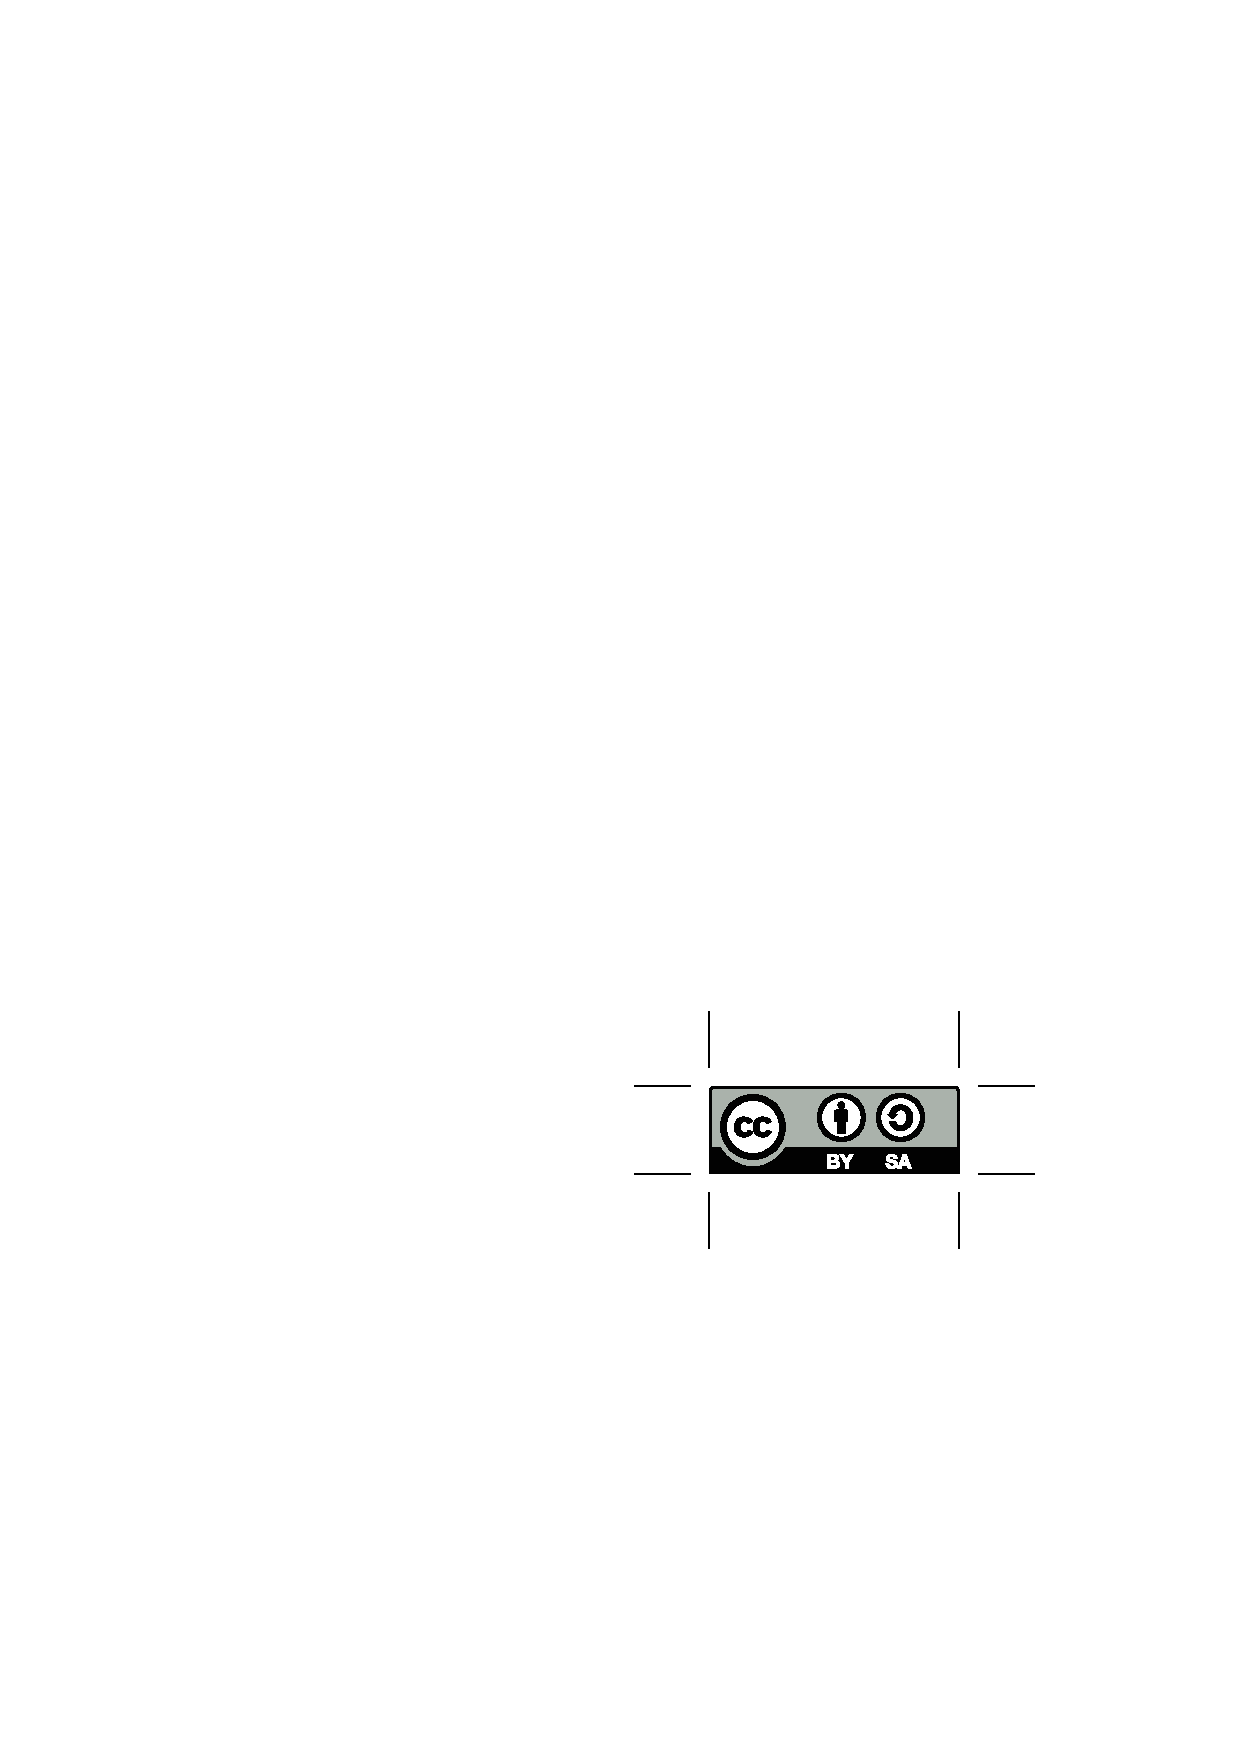
\includegraphics[height=1cm]{by-sa}} Patty C. Hill and Jason L. Ermer, 2014

\copyright{2014} by Patty C. Hill and Jason L. Ermer. Untitled Algebra Book is licensed under the Creative Commons Attribution-ShareAlike 4.0 International License.

To view a copy of this license, visit \url{http://creativecommons.org/licenses/by-sa/4.0/}.
\clearpage

%%% % % % % % % % % % % % % % % % % % % % % % % % % % % % % % % % % % % %
%%% Front matter
\frontmatter
\pagestyle{plain}
%\pagenumbering{roman}

%%% Table of contents
\setcounter{tocdepth}{1}
\tableofcontents

%%% Acknowledgements
\chapter{Acknowledgements}
\label{ch:acknowledgements}

Who needs thank-yous? Math dep't at Kealing... magnet directors (Hovland, Goka, Ramberg)... a general shout out to all of our students over the years? MTCA folks?

Also: should we try to recruit an editor w/ a mathematics background? Altha and Adriana both come to mind...

Thanks to Shawn Tyson for editing help. The serial comma was always a given, naturally, but who knew that ``logical punctuation'' was a thing?

This book was typeset using \LaTeX, so we want to thank the many program and package authors, designers, and maintainers whose work has made that possible. Thanks also to the online \LaTeX\ community, in particular all those who have posed and answered questions at \href{http://tex.stackexchange.com/}{tex.stackexchange.com}.

The cover image ``\href{http://subtlepatterns.com/black-scales/}{black scales}'' was designed by \href{https://twitter.com/misterparker}{Alex Parker} and made available through the website \href{http://subtlepatterns.com/}{Subtle Patterns by Atle Mo}, under the \href{http://creativecommons.org/licenses/by-sa/3.0/}{CC BY-SA 3.0 license}.


%%% % % % % % % % % % % % % % % % % % % % % % % % % % % % % % % % % % % %
%%% Main document
\mainmatter
\pagestyle{fancy}
%\pagenumbering{arabic}

\lhead{}
\rhead{\leftmark}
\cfoot{\thepage}
%\rfoot{\ifnum\thepage=6{This is page 6!}\fi}

%%% Glossary definitions

\newglossaryentry{abscissa} {
	name=abscissa,
	description={The x-coordinate of a point in the coordinate plane.}
}

\newglossaryentry{absolute value} {
	name=absolute value,
	description={For real numbers, it is the distance a number is away from zero on a number line. It is a scalar quantity, meaning it just has a magnitude and no direction (sign). The absolute value of a number is always non-negative. In the order of 
operations, it works like a grouping symbol. The ``absolute value of x'' is denoted $\abs{x}$.}
}

\newglossaryentry{addition property of equality} {
	name=addition property of equality,
	description={For all real numbers $a$, $b$, and $c$: If $a = b$, then $a + c = b + c$. This axiom is used when solving equations. }
}

\newglossaryentry{addition property of order} {
	name=addition property of order,
	description={For all real numbers $a$, $b$, and $c$: If $a > b$, then $a + c > b + c$. This axiom is used when solving inequalities and also applies to inclusive 
symbols of order. }
}

\newglossaryentry{additive identity} {
	name=additive identity,
	description={The number which, when added to a given number $x$, leaves $x$ unchanged. In the real number system, 0 is the additive identity. The existence of the additive identity is a \gls{field axiom}.}
}

\newglossaryentry{additive inverse} {
	name=additive inverse,
	description={The number which, when added to a given number $x$, gives a sum of 0, the additive identity. The opposite of a number is its additive inverse. The existence of the additive inverse is a \gls{field axiom}.}
}

\newglossaryentry{algebraic expression} {
	name=algebraic expression,
	description={A symbolic representation of mathematical operations that can involve both numbers and variables. There is no equal sign in an expression.}
}

\newglossaryentry{algebraic number} {
	name=algebraic number,
	description={A number that is the root on a nonzero polynomial equation in one variable with rational coefficients. The set of algebraic numbers is a subset of the real numbers.}
}

\newglossaryentry{arithmetic sequence} {
	name=arithmetic sequence,
	description={A sequence where the difference between each pair of successive terms is constant. The constant difference is called the ``common difference'', usually denoted $d$.}
}

\newglossaryentry{associative property of addition} {
	name=associative property of addition,
	description={For all real numbers $a$, $b$, and $c$: $a + (b + c) = (a + b) + c$. This field axiom allows for the regrouping of longer strings of addition.}
}

\newglossaryentry{associative property of multiplication} {
	name=associative property of multiplication,
	description={For all real numbers $a$, $b$, and $c$: $a (b c) = (a b) c$. This field axiom allows for the regrouping of longer strings of multiplication.}
}

\newglossaryentry{asymptote} {
	name=asymptote,
	description={A line that a curve approaches as they both tend towards infinity. There are three types of asymptotes: vertical, horizontal, and oblique (slant). Exponential functions have a horizontal asymptote.}
}

\newglossaryentry{axiom} {
	name=axiom,
	description={A property or statement that is accepted without proof.}
}

\newglossaryentry{axis} {
	name=axis,
	plural=axes,
	description={One of two perpendicular number lines used to locate points in the coordinate plane. The plural form is ``axes''.}
}

\newglossaryentry{axis of symmetry} {
	name=axis of symmetry,
	plural=axes of symmetry,
	description={The line about which one can reflect an image onto itself. For example, a parabola has an axis of symmetry. Given the graph of a quadratic function, the axis of symmetry is a vertical line through the vertex. When written in standard form, the equation for the line of symmetry is given by $x = -\frac{b}{2a}$.}
}

\newglossaryentry{base} {
	name=base,
	description={(1) For triangles: A side of the triangle. (2) For expressions: A term or expression that is raised to a power.}
}

\newglossaryentry{binomial} {
	name=binomial,
	description={A polynomial with exactly 2 terms.}
}

\newglossaryentry{boundary} {
	name=boundary,
	description={For a one-variable \gls{inequality}, the boundary is a point on the number line. Inclusive boundaries are drawn as closed or filled in points, and exclusive boundaries are draw as open circles. For a two-variable inequality, the boundary is a line or curve. Inclusive boundaries are drawn as solid 
lines/curves, and exclusive boundaries are lines/curves drawn with a dashed or dotted line. For a linear inequalities, the boundary line separates the plane into two \glspl{half-plane}, one of which will contain the solutions to the inequality.}
}

\newglossaryentry{Cartesian plane} {
	name=Cartesian plane,
	description={See \gls{coordinate plane}.}
}

\newglossaryentry{closure} {
	name=closure,
	description={A set is said to be to ``have closure'' (or to ``be closed'') under an operation performing the operation on members from the set always yields a result that is also a member of the set. The \glspl{natural number}, for example, are closed under the operation of addition, since the sum of any two natural numbers is itself a natural number. The natural numbers are not closed under the operation of subtraction.}
}

\newglossaryentry{coefficient} {
	name=coefficient,
	description={The numerical factor in a term with a variable. If the number is not explicitly written, the coefficient is understood to be 1.}
}

\newglossaryentry{colinear} {
	name=colinear,
	description={To be on the same line.}
}

\newglossaryentry{combining like terms} {
	name=combining like terms,
	description={A short-cut used to add terms that have exactly the same variables raised to the same exponents.}
}

\newglossaryentry{common monomial factor} {
	name=common monomial factor,
	description={A monomial that is a factor of every term in a polynomial expression.}
}

\newglossaryentry{common difference} {
	name=common difference,
	description={In an arithmetic sequence, it is the constant difference between successive terms.}
}

\newglossaryentry{common ratio} {
	name=common ratio,
	description={In an geometric sequence, it is the constant ratio between successive terms.}
}

\newglossaryentry{commutative property of addition} {
	name=commutative property of addition,
	description={For all real numbers $a$ and $b$: $a + b = b + a$. This field axiom allows for the reordering longer strings of addition. }
}

\newglossaryentry{commutative property of multiplication} {
	name=commutative property of multiplication,
	description={For all real numbers $a$ and $b$: $a b = b a$. This field axiom allows for the reordering longer strings of multiplication. }
}

\newglossaryentry{completing the square} {
	name=completing the square,
	description={Using the properties of equality on a quadratic equation to convert one side into a perfect square trinomial. Completing the square can be used as a 
technique to solve quadratic equations.}
}

\newglossaryentry{complex number} {
	name=complex number,
	description={A member of the set of numbers that consists of real and imaginary numbers. The set is denoted $\C$.}
}

\newglossaryentry{compound interest} {
	name=compound interest,
	description={A way to calculate interest based on both the principal amount and any interest already accrued. This type of interest is an exponential relationship. The formula is $A = P \left(1 + \frac{r}{n} \right)^{nt}$, where $P$ is the principal amount, $r$ is the rate of interest, $t$ is the amount of time over which interest is to be computed, and $n$ is the number of compounding periods per unit of time.}
}

\newglossaryentry{constant} {
	name=constant,
	description={A value that does not change.}
}

\newglossaryentry{constant function} {
	name=constant function,
	description={A function whose graph is a horizontal line. It is of the form $f(x) = c$, where $c$ is a constant. Constant functions are polynomial functions of degree zero.}
}

\newglossaryentry{constant multiplier} {
	name=constant multiplier,
	description={In a sequence that grows or decays exponentially, the number each term is multiplied by to get the next term. Also known as the ``common multiplier'', or ``common ratio''.}
}

\newglossaryentry{constant of variation} {
	name=constant of variation,
	description={The constant ratio in a direct variation or the constant product in an inverse variation. It is designated with the variable $k$.}
}

\newglossaryentry{constant term} {
	name=constant term,
	description={A term that includes no variable.}
}

\newglossaryentry{constraint} {
	name=constraint,
	description={The limitations on the values of the variables in a problem. Equations, inequalities and systems are used model the constraints in real-world situations.}
}

\newglossaryentry{continuous data} {
	name=continuous data,
	description={Data that has no breaks and has measurements that can change between data points. Graphically, the measured data points are connected with lines or curves.}
}

\newglossaryentry{continuous function} {
	name=continuous function,
	description={A function that has no breaks in the domain or range. The graph of a continuous function is a line or curve with no holes, gaps, or vertical asymptotes.}
}

\newglossaryentry{converse of the Pythagorean theorem} {
	name=converse of the Pythagorean theorem,
	description={If a triangle has sides $a$, $b$, and $c$, such that $a^2+b^2=c^2$, then the triangle is a right triangle with a hypotenuse of length $c$.}
}

\newglossaryentry{conversion factor} {
	name=conversion factor,
	description={A ratio used to convert measurement from one unit to another.}
}

\newglossaryentry{coordinate plane} {
	name=coordinate plane,
	description={A plane with a pair of scaled, perpendicular axes allowing one to locate points with ordered pairs and to represent lines and curves by equations. Also known as the Cartesian plane, named for its creator, French philosopher Ren\'{e} Descartes.}
}

\newglossaryentry{coprime} {
	name=coprime,
	description={See \gls{relatively prime}.}
}

\newglossaryentry{correlation} {
	name=correlation,
	description={Used in describing data graphed in a scatter plot. It is a trend between two variables. A trend can show positive, negative, or no correlation. Positive correlation shows an \gls{increasing} trend in data. Negative correlation shows a \gls{decreasing} trend in data.}
}

\newglossaryentry{cubic} {
	name=cubic,
	description={A function, number, or expression raised to the third power. Called cubic as it relates to the volume of a cube.}
}

\newglossaryentry{decay factor} {
	name=decay factor,
	description={In exponential decay, the constant multiplier used to calculate the amount of decay after each unit of time. In the formula $y = (1-r)^x$, it is the quantity $(1-r)$. It represents the quantity remaining and is the common multiplier in the exponential relationship.}
}

\newglossaryentry{decay rate} {
	name=decay rate,
	description={In exponential decay, the fraction or percentage by which a population decreases for each unit of time. In the formula $y = (1-r)^x$, it is the quantity $r$.}
}

\newglossaryentry{decreasing} {
	name=decreasing,
	description={A function is said to be decreasing if as $x$ increases, $y$ decreases. Lines with negative slopes are decreasing.}
}

\newglossaryentry{degree of a polynomial} {
	name=degree of a polynomial,
	description={The degree of the term in a polynomial with the highest degree.}
}

\newglossaryentry{degree of a term} {
	name=degree of a term,
	description={The power (exponent) to which the variable is raised in a variable term. If there is no exponent explicitly written on a variable in a term, the term is understood to be of degree 1. The degree of a constant term is zero.}
}

\newglossaryentry{delta}
{
	name={$\Delta$},
	description={Delta, the fourth letter of the Greek alphabet. Used to represent change. They symbol $\Delta x$ is read ``delta $x$'' or ``the change in $x$''.}
}

\newglossaryentry{denominator} {
	name=denominator,
	description={The number or expression below the \gls{vinculum} in a \gls{rational number} or \gls{rational expression}. For example, in the number $\frac{5}{2}$, the denominator is 2.}
}

\newglossaryentry{dependent variable} {
	name=dependent variable,
	description={A variable whose values depend on the values of another variable. In a graph of the relationship between the two variables, the values on the vertical axis represent the values of the dependent variable. The generic variable used is $y$.}
}

\newglossaryentry{difference of squares} {
	name=difference of squares,
	description={A binomial of the form $a^2-b^2$.}
}

\newglossaryentry{dimensional analysis} {
	name=dimensional analysis,
	description={A strategy for converting a measurement from one unit to another using multiplication by a string of conversion factors. The key is to include the units with the numbers. It is used often in science.}
}

\newglossaryentry{direct variation} {
	name=direct variation,
	description={In Algebra 1, a relationship in which the ratio of two variables is constant. A direct variation has an equation of the form $y = kx$. The quantities represented by $x$ and $y$ are said to be \gls{directly proportional}. The value $k$ is called the \gls{constant of variation}.}
}

\newglossaryentry{directly proportional} {
	name=directly proportional,
	description={Used to describe two variables whose values have a constant ratio.}
}

\newglossaryentry{discrete data} {
	name=discrete data,
	description={Data that can only take on certain values. Discrete data usually involves a count of items.}
}

\newglossaryentry{discrete function} {
	name=discrete function,
	description={A function whose domain and range have breaks or are made up of distinct values rather than intervals of real numbers. The graph of a discrete function will have breaks or will be made up of distinct points.}
}

\newglossaryentry{discriminant} {
	name=discriminant,
	description={The expression under the square root in the quadratic formula, used to determine the number and nature of the roots of a quadratic. If a quadratic equation is written in standard form, then the discriminant is $b^2 - 4ac$. If the value of the discriminant is greater than 0, there are two real solutions to the quadratic equation. If it is equal to zero, there is one real solution. If it is less than zero, there are no real solutions to the quadratic equation.}
}

\newglossaryentry{distance formula} {
	name=distance formula,
	description={A formula based on the Pythagorean theorem that uses the coordinates of two points to calculate the distance between the two points. The formula for the distance $d$ between any two points $(x_1, y_1)$ and $(x_2, y_2)$ is $d = \sqrt{ (x_2 - x_1)^2 + (y_2 - y_1)^2 }$.}
}

\newglossaryentry{distributive property} {
	name=distributive property,
	description={For all real numbers $a$, $b$, and $c$: $a (b + c) = ab + ac$. This field axiom allows one to simplify an expression without having the evaluate the sum inside the grouping symbol first.}
}

\newglossaryentry{division property of equality} {
	name=division property of equality,
	description={For all real numbers $a$, $b$, and $c$, where $c \neq 0$: if $a = b$, then $\frac{a}{c} = \frac{b}{c}$. This property is a version of the multiplication property of equality. It is used when solving equations.}
}

\newglossaryentry{division property of order} {
	name=division property of order,
	description={For all real numbers $a$, $b$, and $c$ where $c>0$: if $a < b$, then $\frac{a}{c} < \frac{b}{c}$. If, on the other hand, $c<0$, then $a < b$ implies $\frac{a}{c} > \frac{b}{c}$. This property is a version of the multiplication property of order. It is used when solving inequalities.}
}

\newglossaryentry{domain} {
	name=domain,
	description={The set of all input values of a function, or the $x$-values. In a problem context it is represented by the independent variable.}
}

\newglossaryentry{domain restriction} {
	name=domain restriction,
	description={Values that cannot be used in the domain of a function. Radical and rational functions have domain restrictions.}
}

\newglossaryentry{doubling time} {
	name=doubling time,
	description={In exponential growth, the amount of time it takes for a population, or amount, to double in size. It is constant for an exponential relationship.}
}

\newglossaryentry{elimination method} {
	name=elimination method,
	description={A method for solving a system of equations that involves adding or subtracting multiples of the equations in order to eliminate a variable. It is based on Gaussian Elimination, a method to solve systems of equations that have been converted into matrices.}
}

\newglossaryentry{equation} {
	name=equation,
	description={A statement that says the value of one expression is the same as the value of another expression.}
}

\newglossaryentry{equivalent equations} {
	name=equivalent equations,
	description={Equations that have the same solution set.}
}

\newglossaryentry{equivalent inequalities} {
	name=equivalent inequalities,
	description={Inequalities that have the same solution set.}
}

\newglossaryentry{evaluate} {
	name=evaluate,
	description={To find the value of an expression. If an expression contains variables, values must be substituted for the variable before the expression can be evaluated.}
}

\newglossaryentry{exclusive boundary} {
	name=exclusive boundary,
	description={See \gls{boundary}.}
}

\newglossaryentry{exclusive inequality} {
	name=exclusive inequality,
	description={See \gls{inequality}.}
}

\newglossaryentry{exponent} {
	name=exponent,
	description={A number or variable written as a small superscript to a number or a variable, called the \gls{base}, that indicates how many times the base is being used as a factor.}
}

\newglossaryentry{expanded form} {
	name=expanded form,
	description={The form of an exponential expression in which repeated multiplication is written out. For example, the right-hand side of the equation $x^3 = x\cdot x \cdot x$, is written in expanded form.}
}

\newglossaryentry{exponential decay} {
	name=exponential decay,
	description={A decreasing pattern in which amounts decrease by a constant percent.}
}

\newglossaryentry{exponential equation} {
	name=exponential equation,
	description={An equation in which a variable appears in the exponent.}
}

\newglossaryentry{exponential form} {
	name=exponential form,
	description={The form of an expression in which repeated multiplication is written using an exponent. For example, the left-hand side of the equation $x^3 = x\cdot x \cdot x$, is written in exponential form.}
}

\newglossaryentry{exponential function} {
	name=exponential function,
	description={A function that repeatedly multiplies an initial amount by the same positive number. They can all be modeled using $y = ab^x$ where $a$ is the initial amount and $b$ is the constant multiplier.}
}

\newglossaryentry{exponential growth} {
	name=exponential growth,
	description={An increasing pattern in which amounts increase by a constant percent.}
}

\newglossaryentry{extraneous solution} {
	name=extraneous solution,
	description={An apparent solution of an equation that does not satisfy the original equation. They occur when the transformation of an equation changes the solution set of the original equation, for example squaring both sides of an equation or multiplying by a quantity that can be zero.}
}

\newglossaryentry{factor} {
	name=factor,
	description={One of the numbers, variables, or expressions multiplied to obtain a product.}
}

\newglossaryentry{factored form} {
	name=factored form,
	description={The form of an expression when it is written as the product of factors. The factors can be numbers, variables, or expressions. Factored form is not simplified.}
}

\newglossaryentry{factoring} {
	name=factoring,
	description={The process of rewriting an expression as a product of factors.}
}

\newglossaryentry{family of functions} {
	name=family of functions,
	plural=families of functions,
	description={Similar functions that are all transformations of the same parent function.}
}

\newglossaryentry{field axiom} {
	name=field axiom,
	description={One of a set of axioms including closure, identity, inverse, associative, commutative, and distributive properties. Along with a few definitions and properties of equality, they create the foundation upon which algebra is built.}
}

\newacronym{FOIL}{FOIL}{A mnemonic for remembering the procedure to multiply two binomials. F stands for multiplying the first term in each binomial. O stands for multiplying the outer terms of the binomials. I stands for 
multiplying the inner terms of the binomials. L stands for multiplying that last 
term in each binomial.}

\newglossaryentry{fractal} {
	name=fractal,
	description={A geometric figure that has undergone infinite applications of a recursive procedure and which exhibits the property of self-similarity. }
}

\newglossaryentry{function} {
	name=function,
	description={A relation in which there is exactly one output value for each input value. The graph of a function must pass the vertical line test.}
}

\newglossaryentry{function notation} {
	name=function notation,
	description={A notation in which a function is named by a letter and the input is shown in parenthesis after the function name, generically, $f(x)$, read ``$f$ of $x$''. The variables used may be changed to better represent quantities in a problem, for example $d(t)$ may represent distance $d$ as a function of time $t$. When graphing in the \gls{coordinate plane}, $f(x)$ is another way to write $y$. When $x$ is replaced by a number, it indicates that one should evaluate the function at that value. The notation was first used by Swiss mathematician Leonhard Euler.}
}

\newglossaryentry{function rule} {
	name=function rule,
	description={An expression that represents the relationship between the variables of a function.}
}

\newacronym{GCF}{GCF}{Greatest Common Factor}

\newglossaryentry{geometric sequence} {
	name=geometric sequence,
	description={A sequence where the ratio between each pair of successive terms is constant. The constant ratio is called the ``common ratio'', usually denoted $r$. Geometric sequences are exponential.}
}

\newglossaryentry{growth factor} {
	name=growth factor,
	description={In exponential growth, the constant multiplier used to calculate the amount of growth after each unit of time. In the formula $y = (1+r)^x$, it is the quantity $(1+r)$. It is the common multiplier in the exponential relationship.}
}

\newglossaryentry{growth rate} {
	name=growth rate,
	description={In exponential growth, the fraction or percentage by which a population increases for each unit of time. In the formula $y = (1+r)^x$, it is the quantity $r$.}
}

\newglossaryentry{half-life} {
	name=half-life,
	description={The time needed for an amount of a substance to exponentially decay to half the original amount. Half-life is constant for an exponential relationship.}
}

\newglossaryentry{half-plane} {
	name=half-plane,
	description={The set of points on a plane that fall on one side of a boundary line. Part of the solution of a linear inequality in two variables is a half-plane.}
}

\newglossaryentry{hypotenuse} {
	name=hypotenuse,
	description={The side of a right triangle opposite the right angle. It is the longest side of the triangle.}
}

\newglossaryentry{identity} {
	name=identity,
	description={When solving equations with variables on both sides, identities occur when the equation is true for every value of the variable. The solution set $S$ is written as $S=\R$.}
}

\newglossaryentry{identity property of addition} {
	name=identity property of addition,
	description={The sum of any number and 0 is that number. For every real number $a$, $a + 0 = a$ and $0 + a = a$. The existence of the \gls{additive identity} is a \gls{field axiom}.}
}

\newglossaryentry{identity property of multiplication} {
	name=identity property of multiplication,
	description={The product of any number and 1 is that number. For every real number $a$, $a \cdot 1 = a$ and $1 \cdot a = a$. The existence of the multiplicative identity is a \gls{field axiom}.}
}

\newglossaryentry{imaginary number} {
	name=imaginary number,
	description={A member of the set of numbers that is created by taking the square root of a negative number. In the set of imaginary numbers, the square root of -1 is represented by the letter $i$. The set of imaginary numbers is a subset of the complex number system. The sets of real and imaginary numbers are disjoint, meaning they have no common members.}
}

\newglossaryentry{implied operation} {
	name=implied operation,
	description={An operation that is not explicitly written. For example, in $3 (x + 4)$ the multiplication between 3 and $(x + 4)$ is an implied operation, since no multiplication symbol is explicitly written in between.}
}

\newglossaryentry{improper fraction} {
	name=improper fraction,
	description={A fraction whose \gls{numerator} is greater than its \gls{denominator}. For example, $\frac{5}{2}$ is an improper fraction. A fraction that is not an improper fraction is called a \gls{proper fraction}. See also \gls{mixed number}.}
}

\newglossaryentry{increasing} {
	name=increasing,
	description={A function is said to be decreasing if as $x$ increases, $y$ increases. Lines with positive slopes are decreasing.}
}

\newglossaryentry{independent variable} {
	name=independent variable,
	description={A variable whose values affect the values of another variable. In a graph of the relationship between the two variables, the values on the horizontal axis represent the values of the dependent variable. The generic variable used is $x$.}
}

\newglossaryentry{inequality} {
	name=inequality,
	description={A statement that one quantity is less than or greater than another. An inequality may exclusive or inclusive. The exclusive inequalities are $<$ and $>$, read ``less than'' and ``greater than''. The inclusive inequalities are $\leq$ and $\geq$, read ``less than or equal to'' and ``greater than or equal to''.}
}

\newglossaryentry{initial value} {
	name=initial value,
	description={The starting value of a sequence or exponential function.}
}

\newglossaryentry{integer} {
	name=integer,
	description={A member of the set of natural numbers, their opposites, and zero. The set is denoted $\Z$, and we may write $\Z = \{0, \pm1, \pm2, \pm3, \dotsc \}$. The integers are a subset of the rational numbers.}
}

\newglossaryentry{inclusive boundary} {
	name=inclusive boundary,
	description={See \gls{boundary}.}
}

\newglossaryentry{inclusive inequality} {
	name=inclusive inequality,
	description={See \gls{inequality}.}
}

\newglossaryentry{intercept} {
	name=intercept,
	description={The point which a graph intersects one of the axes.}
}

\newglossaryentry{interest} {
	name=interest,
	description={A percentage of the balance added to an account at regular time intervals.}
}

\newglossaryentry{interest rate} {
	name=interest rate,
	description={The percentage used to calculate interest.}
}

\newglossaryentry{inverse property of addition} {
	name=inverse property of addition,
	description={For any real number $a$, there exists a real number $\umin a$ such that $a + \umin a = 0$. The number $\umin a$ is called the \gls{additive inverse} of $a$. Very often we will call it the \gls{opposite} of $a$.}
}

\newglossaryentry{inverse property of multiplication} {
	name=inverse property of multiplication,
	description={For any nonzero real number $a$, there exists a real number $\frac{1}{a}$ such that $a \cdot \frac{1}{a} = 1$. The number $\frac{1}{a}$ is called the \gls{multiplicative inverse} of $a$. Very often we will call it the \gls{reciprocal} of $a$.}
}


\newglossaryentry{inverse variation} {
	name=inverse variation,
	description={In Algebra 1, a relationship in which the product of two variables is constant. An inverse variation has an equation in the form $xy = k$, or $y = \frac{k}{x}$. The quantities represented by $x$ and $y$ are said to be \gls{inversely proportional}. The value $k$ is called the \gls{constant of variation}.}
}

\newglossaryentry{inversely proportional} {
	name=inversely proportional,
	description={Used to describe two variables whose values have a constant product.}
}

\newglossaryentry{irrational number} {
	name=irrational number,
	description={A number that cannot be expressed as the ratio of two integers. In decimal form, an irrational number has an infinite number of digits and does not repeat. The set of irrational numbers consist of algebraic and transcendental numbers. The set of irrational numbers is a subset of the real numbers.}
}

\newglossaryentry{irreversible operation} {
	name=irreversible operation,
	description={An operation performed when solving an equation that changes the solution set of the equation. Multiplying or dividing both sides of an equation by an expression that might equal zero are considered irreversible operations.}
}

\newglossaryentry{leg} {
	name=leg,
	description={One of the perpendicular sides of a right triangle.}
}

\newglossaryentry{like terms} {
	name=like terms,
	description={Terms with exactly the same variable factors in a variable expression. The variables and the powers to which the variables are raised must be identical for the terms to be considered like terms.}
}

\newglossaryentry{limited domain} {
	name=limited domain,
	description={The restricted domain of a function. Domains are usually limited in real world contexts. For example, we rarely allow negative values for a variable that represents ``time''. For this reason it is often referred to as a reasonable domain.}
}

\newglossaryentry{line of best fit} {
	name=line of best fit,
	description={A line used to model a set of data. A line of best fit shows general direction of the data. When hand-drawn, one should have about the same number of data points above and below the line. When using the linear regression tool on the 
calculator, the correlation coefficient will show how well the line fits the data.}
}

\newglossaryentry{line of symmetry} {
	name=line of symmetry,
	description={See \gls{axis of symmetry}.}
}

\newglossaryentry{linear} {
	name=linear,
	description={In the shape of a line or represented by a line. In mathematics, a linear equation or expression has variables raised only to the power of 1.}
}

\newglossaryentry{linear function} {
	name=linear function,
	description={A function characterized by a constant rate of change. The graph of a linear function is a non-vertical line. It is a polynomial of degree one.}
}

\newglossaryentry{linear inequality} {
	name=linear inequality,
	description={An inequality of two variables whose boundary is formed by a linear function. It describes a region of the coordinate plane that consists of a boundary line and a half-plane.}
}

\newglossaryentry{linear programming} {
	name=linear programming,
	description={A method to optimize a quantity that uses an objective function to represent the quantity and a system of linear inequalities to represent the constraints on the variables involved. The system of inequalities are graphed to represent a set of feasible solutions and the vertices of the region will describe the optimal amount of the quantity.}
}

\newglossaryentry{linear relationship} {
	name=linear relationship,
	description={A relationship that can be represented by a linear function. A linear relationship is characterized by a constant rate of change.}
}

\newglossaryentry{linear term} {
	name=linear term,
	description={A term of degree 1.}
}

\newglossaryentry{lowest terms} {
	name=lowest terms,
	description={The form of a fraction in which the numerator and denominator are \gls{relatively prime}. A fraction in lowest terms is also called a reduced fraction.}
}

\newglossaryentry{mapping diagram} {
	name=mapping diagram,
	description={A diagram used to determine if a relation is a function. The values of the domain and range are written in circles. Arrows are drawn from the elements of the domain to the corresponding elements of the range. It is a visual that shows 
how the members of the domain map to the members of the range.}
}

\newglossaryentry{mathematical equivalence} {
	name=mathematical equivalence,
	description={The idea that numbers, expressions, equations, functions, or other mathematical objects can be algebraically manipulated, using specific rules, such that their representations and appearance are changed while other fundamental properties remain unchanged.}
}

\newglossaryentry{mathematical modeling} {
	name=mathematical modeling,
	description={Translating a real-world scenario with a given set of constraints into an abstract representation that can be manipulated and studied mathematically. For example, creating a set of variables and equations to solve a \gls{linear programming} problem.}
}

\newglossaryentry{maximum} {
	name=maximum,
	description={The greatest value. In a quadratic function, the vertex will be a maximum if the coefficient of the quadratic term is negative.}
}

\newglossaryentry{midpoint} {
	name=midpoint,
	description={The point on a line segment halfway between the endpoints. The coordinates of the midpoint are found by averaging the abscissas and ordinates of the endpoints.}
}

\newglossaryentry{midpoint formula} {
	name=midpoint formula,
	description={The formula that can be used to compute the midpoint of a line segment. Given a line segment with endpoints $(x_1, y_1)$ and $(x_2, y_2)$, the midpoint of the segment has coordinates $\left( \frac{x_1+x_2}{2}, \frac{y_1+y_2}{2} \right)$.}
}

\newglossaryentry{minimum} {
	name=minimum,
	description={The smallest value. In a quadratic function, the vertex will be a minimum if the coefficient of the quadratic term is positive.}
}

\newglossaryentry{mixed number} {
	name=mixed number,
	description={The sum of a nonzero \gls{integer} and a \gls{proper fraction}. For example $2\frac{3}{5}$ is a mixed number. See also \gls{improper fraction}.}
}

\newglossaryentry{monomial} {
	name=monomial,
	description={A polynomial with only one term.}
}

\newglossaryentry{multiplication property of equality} {
	name=multiplication property of equality,
	description={For all real numbers $a$, $b$, and $c$: if $a = b$ then $ac = bc$. This property is used to solve equations.}
}

\newglossaryentry{multiplication property of order} {
	name=multiplication property of order,
	description={For all real numbers $a$, $b$, and $c$ and $c > 0$: if $a < b$ then $ac < bc$. If, on the other hand, $c < 0$, then $a < b$ implies $ac > bc$. This property is used to solve equations.}
}

\newglossaryentry{multiplicative identity} {
	name=multiplicative identity,
	description={The number which, when multiplied by a given number $x$, leaves $x$ unchanged. In the real number system, 1 is the multiplicative identity. The existence of the multiplicative identity is a \gls{field axiom}.}
}

\newglossaryentry{multiplicative inverse} {
	name=multiplicative inverse,
	description={The number which, when multiplied by a given nonzero number $x$, gives a product of 1, the multiplicative identity. The reciprocal of a number is its multiplicative inverse. The existence of the multiplicative inverse is a \gls{field axiom}.}
}

\newglossaryentry{natural number} {
	name=natural number,
	description={A member of the set $\{1, 2, 3, 4, \dotsc\}$, denoted $\N$. Also called the counting numbers. The number 0 is sometimes included as a natural number.}
}

\newglossaryentry{negative correlation} {
	name=negative correlation,
	description={See \gls{correlation}.}
}

\newglossaryentry{null set} {
	name=null set,
	description={A set that contains no elements. Also called the empty set. Used to show that there is no solution to an equation. Denoted $\emptyset$ or $\{ \}$.}
}

\newglossaryentry{numerator} {
	name=numerator,
	description={The number or expression above the \gls{vinculum} in a \gls{rational number} or \gls{rational expression}. For example, in the number $\frac{5}{2}$, the numerator is 5.}
}

\newglossaryentry{numeric expression} {
	name=numeric expression,
	description={An expression containing only numbers and mathematical operations.}
}

\newglossaryentry{obelus} {
	name=obelus,
	symbol={$\div$},
	description={The division symbol $\div$.}
}

\newglossaryentry{one-variable data} {
	name=one-variable data,
	description={Data that measures only one trait or quantity. A one-variable data set consists of single values (as opposed to ordered pairs) and is graphed on a number line. Compare with: \gls{two-variable data}.}
}

\newglossaryentry{opposite} {
	name=opposite,
	description={See \gls{additive inverse}.}
}

\newglossaryentry{optimization} {
	name=optimization,
	description={To maximize or minimize a quantity given constraints. For example a company will want to optimize (maximize) their profits while faced with constraints such as the cost and availability of labor and materials.}
}

\newglossaryentry{order of magnitude} {
	name=order of magnitude,
	description={A way of expressing the size of an very large or very small number by giving the power of 10 associated with the number.}
}

\newglossaryentry{order of operations} {
	name=order of operations,
	description={The agreed-upon order in which operations are carried out when evaluating an expression.}
}

\newglossaryentry{ordered pair} {
	name=ordered pair,
	description={A pair of numbers named in an order that matters. The coordinates of a point are given as an ordered pair in which the first number is the $x$-coordinate (abscissa) and the second number is the $y$-coordinate (ordinate).}
}

\newglossaryentry{ordinate} {
	name=ordinate,
	description={The y-coordinate of a point in the coordinate plane.}
}
  
\newglossaryentry{origin} {
	name=origin,
	description={The point where the coordinate axes intersect. In a coordinate plane it has the coordinates $(0,0)$.}
}

\newglossaryentry{parabola} {
	name=parabola,
	description={The set of all points whose distance from a fixed point (called the focus) is equal to the distance from a fixed line (called the directrix). Also known as the smooth ``U'' shaped curve of a quadratic function.}
}

\newglossaryentry{parallel lines} {
	name=parallel lines,
	description={Lines in the same plane that never intersect. They are always the same distance apart in Euclidean geometry. The slopes of parallel lines are the same.}
}

\newglossaryentry{parent function} {
	name=parent function,
	description={The most basic form of a function. A parent function can be transformed to create a family of functions.}
}

\newglossaryentry{percent change} {
	name=percent change,
	description={The percent by which an amount differs from its original amount. It is calculated by taking the amount of the change and dividing it by the original amount.}
}

\newglossaryentry{perfect cube} {
	name=perfect cube,
	description={A number that is equal to the cube of an integer, or a polynomial that is equal to the cube of another polynomial.}
}

\newglossaryentry{perfect square} {
	name=perfect square,
	description={A number that is equal to the square of an integer, or a polynomial that is equal to the square of another polynomial.}
}

\newglossaryentry{perfect square trinomial} {
	name=perfect square trinomial,
	description={A trinomial generated by squaring a binomial. For example, squaring the binomial $(a+b)$ yields $(a+b)^2 = a^2 + 2ab + b^2$. Thus, $a^2 + 2ab + b^2$ is a perfect square trinomial.}
}

\newglossaryentry{period of compounding} {
	name=period of compounding,
	description={The number of times interest is calculated during a year for compound interest. It is represented by $n$ in the \gls{compound interest} formula.}
}

\newglossaryentry{perpendicular lines} {
	name=perpendicular lines,
	description={Lines that intersect at a right angle. The slopes of perpendicular lines are opposites and reciprocals. The slopes of perpendicular lines multiply to $-1$.}
}

\newglossaryentry{point-slope form} {
	name=point-slope form,
	description={The form of a linear equation that uses the slope and any point on the line. It is written either $y-y_1 = m(x-x_1)$ or $y=m(x-x_1)+y_1$, where $m$ is the slope of the line and $(x_1,y_1)$ is a point on the line. It can be derived from the slope formula and represents the transformation of the line $y = mx$ where a vertical shift of $y_1$ and a horizontal shift of $x_1$ has occurred.}
}

\newglossaryentry{polynomial} {
	name=polynomial,
	description={A sum of terms that have positive integer exponents. In Algebra 1, all polynomials are in one variable.}
}

\newglossaryentry{positive correlation} {
	name=positive correlation,
	description={See \gls{correlation}.}
}

\newglossaryentry{principal amount} {
	name=principal amount,
	description={The original amount invested in a situation that involves accumulating interest. It is represented by $P$ in the \gls{compound interest} and simple interest formulas.}
}

\newglossaryentry{principal square root} {
	name=principal square root,
	description={The positive square root of a number.}
}

\newglossaryentry{proper fraction} {
	name=proper fraction,
	description={A fraction whose \gls{numerator} is less than its \gls{denominator}. For example, the fraction $\frac{7}{9}$ is a proper fraction. A fraction that is not a proper fraction is called an \gls{improper fraction}.}
}

\newglossaryentry{proportion} {
	name=proportion,
	description={An equation stating that two ratios are equal.}
}

\newglossaryentry{power} {
	name=power,
	description={An expression of the form $a^n$ is called a power of $a$.}
}
 
\newglossaryentry{Pythagorean theorem} {
	name=Pythagorean theorem,
	description={A formula that expresses the relationship between the sides of a right triangle. It states that the sum of the squares of the legs of a right triangle is equal to the square of the \gls{hypotenuse}.}
}

\newglossaryentry{quadrangle method} {
	name=quadrangle method,
	description={A technique for solving quadratic equations that is based on the symmetry of the square. When executing the quadrangle method, we often draw a \textit{quadrangle diagram}.}
}

\newglossaryentry{quadrant} {
	name=quadrant,
	description={One of the four regions that a coordinate plane is divided into by the two axes. The quadrants are numbered I, II, III, and IV, starting in the upper right and moving counterclockwise.}
}

\newglossaryentry{quadratic formula} {
	name=quadratic formula,
	description={The formula used to find the exact solution to any quadratic equation. Given that $ax^2+bx+c=0$, the formula states \[x = \frac{-b \pm \sqrt{b^2 - 4ac}}{2a}\] It is derived by completing the square on the standard form quadratic equation.}
}

\newglossaryentry{quadratic function} {
	name=quadratic function,
	description={A function with an equation of the form $y = ax^2 + bx + c$ where $a \neq 0$. The graph of a quadratic function is a \gls{parabola}.}
}

\newglossaryentry{quadratic term} {
	name=quadratic term,
	description={A term of degree 2.}
}

\newglossaryentry{radical} {
	name=radical,
	description={The root symbol $\sqrt{~}$, used to denote square roots, cube roots, and so on. The symbol $\sqrt[n]{x}$ is read ``nth root of x.'' If $n$ is not stated, as in $\sqrt{x}$, it is understood to be 2 and the radical indicates the square root.}
}

\newglossaryentry{radical expression} {
	name=radical expression,
	description={An expression containing a radical (square root, cube root, or any $n$th root).}
}

\newglossaryentry{radical function} {
	name=radical function,
	description={A function where the independent variable is under a radical (square root, cube root, or any $n$th root).}
}

\newglossaryentry{radioactive decay} {
	name=radioactive decay,
	description={The process by which an unstable element loses mass with a release of energy, transforming it into a different element or isotope.}
}

\newglossaryentry{range} {
	name=range,
	description={(1) In statistics it is the difference between the greatest value in a data set and the smallest value in a data set. (2) In the study of functions it is the set of all output values of a function. It is represented by the dependent variable.}
}

\newglossaryentry{rate} {
	name=rate,
	description={A \gls{ratio} that measures two quantities with different units.}
}

\newglossaryentry{rate of change} {
	name=rate of change,
	description={A measurement of how quickly one quantity changes relative to another quantity. Given values $(x_1,y_1)$ and $(x_2,y_2)$, the rate of change of $y$ with respect to $x$ is $\frac{\Delta y}{\Delta x} = \frac{y_2-y_1}{x_2-x_1}$. The patterns of the rate of change of a set of data can be used to determine what type of data is represented by the pattern. For example, the rate of change of linear data is constant.}
}

\newglossaryentry{ratio} {
	name=ratio,
	description={A comparison between two quantities, often written in fraction form.}
}

\newglossaryentry{rational expression} {
	name=rational expression,
	description={An expression that can be written as a ratio of two polynomials. The value of the variable cannot make the denominator 0.}
}

\newglossaryentry{rational function} {
	name=rational function,
	description={A function that is expressed as the ratio of two polynomial expressions. The values of the independent variables that make the denominator zero are restricted from the domain.}
}

\newglossaryentry{rational number} {
	name=rational number,
	description={A number that can be written as a ratio of two integers $\frac{a}{b}$ where $b \neq 0$. Their decimal forms are either terminating or repeating. The set of rational numbers is denoted $\Q$. The rational numbers are a subset of the real numbers.}
}

\newglossaryentry{rationalizing the denominator} {
	name=rationalizing the denominator,
	description={The process of making the denominator of a fraction a rational number without changing the value of the expression. It is used to eliminate a radical from the denominator of a fraction.}
}

\newglossaryentry{real number} {
	name=real number,
	description={Denoted $\R$, the set of real numbers include the integers, rational numbers, and irrational numbers, but not imaginary numbers. This is the number set used in Algebra 1. The set is closed under the operations of addition and multiplication. Members can be graphed on the standard number line.  The real numbers is a subset of the complex numbers.}
}

\newglossaryentry{reciprocal} {
	name=reciprocal,
	description={The multiplicative inverse. The reciprocal of a given number is the number it must be multiplied by to get 1 (the multiplicative identity). To find the reciprocal of a number, we can write the number as a fraction and then invert the fraction. The reciprocal of $n$ is $\frac{1}{n}$.}
}

\newglossaryentry{recursive} {
	name=recursive,
	description={Describes a procedure that is applied over and over again, starting with a number or a geometric figure, to produce a sequence of numbers or figures. The procedure requires previous entries in the pattern to find subsequent entries.}
}

\newglossaryentry{recursive rule} {
	name=recursive rule,
	description={Instructions for producing each stage of a sequence from the previous stage. It must include a description of the starting value.}
}

\newglossaryentry{recursive sequence} {
	name=recursive sequence,
	description={An ordered list of numbers defined by a starting value and a recursive rule. We generate a recursive sequence by applying the rule to the starting value, then applying the rule to the resulting value, and so on.}
}

\newglossaryentry{relatively prime} {
	name=relatively prime,
	description={Two numbers are said to be relatively prime (or coprime) if they have no common factors other than 1. For example, 16 and 21 are relatively prime. In contrast, 21 and 24 are not relatively prime, since both numbers are divisible by 3.}
}

\newglossaryentry{relation} {
	name=relation,
	description={Any set of ordered pairs.}
}

\newglossaryentry{repeating decimal} {
	name=repeating decimal,
	description={A decimal representation of a rational number with a digit or group of digits after the decimal point that repeat infinitely.}
}

\newglossaryentry{root} {
	name=root,
	description={A zero or an $x$-intercept of a function.}
}

\newglossaryentry{sample space} {
	name=sample space,
	description={The set of all possible outcomes of a probability experiment.}
}

\newglossaryentry{scatter plot} {
	name=scatter plot,
	description={A two-variable data display in which values on a horizontal axis represent values of one variable and values on the vertical axis represent values of the other variable. The coordinates of each point represent a pair of data values.}
}

\newglossaryentry{scientific notation} {
	name=scientific notation,
	description={A notation in which a number is written as the product of a number greater than or equal to 1 but less than 10, multiplied by an integer power of 10.}
}

\newglossaryentry{sequence} {
	name=sequence,
	description={A function whose domain is the set of positive integers. A sequence is an ordered list of objects, like numbers. The individual objects are called terms. Unlike a set, order matters, and terms may be repeated.}
}

\newglossaryentry{set} {
	name=set,
	description={An unordered collection of items. Often denoted by listing the elements inside a set of braces.}
}

\newglossaryentry{set notation} {
	name=set notation,
	description={Using curly braces $\{$ and $\}$ to designate quantities that belong to a set. Certain sets do not require the use of braces, as they have symbols used to denote them, like the \gls{null set}, the set of \glspl{integer}, and the set of \glspl{real number}.}
}

\newglossaryentry{simple interest} {
	name=simple interest,
	description={Interest calculated using the formula $I = Prt$. The interest is only ever calculated using the initial investment (called the \gls{principal amount}) and show linear growth.}
}

\newglossaryentry{simplify} {
	name=simplify,
	description={Using algebraic laws and properties which maintain equivalence in order to write an answer so that it fits a set of criteria. The criteria depend on what is being simplified.}
}

\newglossaryentry{simplified radical form} {
	name=simplified radical form,
	description={A radical written so that (1) no perfect square factors exist under the radical (2) no fractions are under the radical and (3) there are no radicals in the 
denominator of the fraction.}
}

\newglossaryentry{slope} {
	name=slope,
	description={The measurement of the steepness of a line, or the rate of change of a linear relationship. Often denoted $m$, and referred to as ``rise over run.'' Given points $(x_1, y_1)$ and $(x_2, y_2)$, the slope of the line between the points is calculated as $m = \frac{\Delta y}{\Delta x} = \frac{y_2-y_1}{x_2-x_1}$.}
}

\newglossaryentry{slope-intercept form} {
	name=slope-intercept form,
	description={The form $y = mx +b$ of a linear equation. The value of $m$ is the slope and the value of $b$ is the $y$-intercept. It is the simplified version of \gls{point-slope form}.}
}

\newglossaryentry{solution} {
	name=solution,
	description={A solution to an equation (or inequality) is any value of the variable (or variables) in the equation (or inequality) that make the equation (or inequality) true. The solution to a system of equations (or inequalities) is the set of all of the points common to all equations in the system. If there is no solution, the system is said to be inconsistent. If there are infinitely many solutions to a system, the system is said to be dependent. If there is a single solution, the system is said to be independent. In a system of two equations in two variables, the solution is the intersection point of the two lines.}
}

\newglossaryentry{solution set} {
	name=solution set,
	description={The set of values that make an equation, inequality, or system true.}
}

%\newglossaryentry{solution to an inequality} {
%	name=solution to an inequality,
%	description={Any value or values of the variable(s) in the inequality that make the inequality true.}
%}

\newglossaryentry{solution set notation} {
	name=solution set notation,
	description={One way to denote the solution set to an equation, written as $S = \{ ~solutions~\}$.}
}

%\newglossaryentry{solution to a system of equations} {
%	name=solution to a system of equations,
%	description={All of the points common to all equations in the system. If there is no solution, the system is said to be inconsistent. If there are infinitely many solutions to a system, the system is said to be dependent. If there is a single solution, the system is said to be independent. In a system of two equations in two variables, the solution is the intersection point of the two lines.}
%}

\newglossaryentry{solve} {
	name=solve,
	description={To find the solution set of an equation.}
}

\newglossaryentry{square root} {
	name=square root,
	description={The square root of a number $a$, denoted $\sqrt{a}$, is the number $b$ such that that $b \cdot b = a$. Every positive number has two square roots, a \gls{principal square root} and a negative square root. The set of real numbers is not closed under the operation of square root.}
}

\newglossaryentry{standard form} {
	name=standard form,
	description={(1) For linear equations, it is an equation of the form $Ax + By = C$, in which $A$ and $B$ are not both 0. (2) For a polynomial, it is an expression written such that it is simplified and the terms are written in decreasing order of degree (highest degree term appears first). (3) For quadratic equations, it is an equation of the form $ax^2 + bx + c$, where $a \neq 0$.}
}

\newglossaryentry{subset} {
	name=subset,
	description={A subset is a set that consists entirely of members from another set. If a set $A$ is a subset of a set $B$, then every item in $A$ is in $B$.}
}

\newglossaryentry{substitution} {
	name=substitution,
	description={To replace a quantity with another one that is equivalent.}
}

\newglossaryentry{substitution method} {
	name=substitution method,
	description={A method for solving a system of equations that involves solving one of the equations for one variable and substituting the resulting expression into the other equation. See also: \gls{elimination method}.}
}

\newglossaryentry{subtraction property of equality} {
	name=subtraction property of equality,
	description={For all real numbers $a$, $b$, and $c$: if $a = b$ then $a - c = b - c$. This property is a restatement of the \gls{addition property of equality} and is used to solve equations.}
}

\newglossaryentry{subtraction property of order} {
	name=subtraction property of order,
	description={For all real numbers $a$, $b$, and $c$: If $a > b$, then $a - c > b - c$. This property is a restatement of the \gls{addition property of order} and is used to solve inequalities.}
}

\newglossaryentry{system of equations} {
	name=system of equations,
	description={A set of two or more equations with the same variables. The equations act as constraints on the variables.}
}

\newglossaryentry{system of inequalities} {
	name=system of inequalities,
	description={A set of two or more inequalities with the same variables. The inequalities act as constraints on the variables.}
}

\newglossaryentry{term} {
	name=term,
	description={An algebraic expression that represents only multiplication and division between variables and constants.}
}

\newglossaryentry{terminating decimal} {
	name=terminating decimal,
	description={A decimal number with a finite number of nonzero digits after the decimal point.}
}

\newglossaryentry{transcendental number} {
	name=transcendental number,
	description={An irrational number that is not algebraic. The number $\pi$ is transcendental because it is not the root of a polynomial equation in one variable with rational coefficients.}
}

\newglossaryentry{trinomial} {
	name=trinomial,
	description={A polynomial with exactly three terms.}
}

\newglossaryentry{turducken} {
	name=turducken,
	description={A food product in which a deboned chicken is stuffed inside a deboned duck, which is then stuffed inside a deboned turkey. In culinary terminology, this is an example of ``engastration'', a cooking method in which one animal is stuffed inside the gastric cavity of another.}
}

\newglossaryentry{two-variable data} {
	name=two-variable data,
	description={A collection of data that measure two traits or quantities. A two-variable data set consists of pairs of values. Compare with: \gls{one-variable data}.}
}

\newglossaryentry{unit rate} {
	name=unit rate,
	description={A ratio in which one of the quantities has the value of 1.}
}

\newglossaryentry{unknown} {
	name=unknown,
	description={A quantity in an equation whose value is not known. In algebra, letters are often used to represent unknowns.}
}

\newglossaryentry{variable} {
	name=variable,
	description={A trait or quantity whose value can change, or vary. In algebra, letters are often used to represent variables.}
}

\newglossaryentry{vector} {
	name=vector,
	description={A quantity that has both a size (or magnitude) and a direction Vectors play an important role in physics and engineering, since many physical quantities (such as velocity, acceleration, and force) are best represented using vectors.}
}

\newglossaryentry{vertex} {
	name=vertex,
	description={Of a parabola, the point where the graph changes direction from increasing to decreasing or from decreasing to increasing.}
}

\newglossaryentry{vertex form} {
	name=vertex form,
	description={A form of a quadratic equation. Given that $(h,k)$ is the vertex, this form is written either as $y-k = a(x-h)^2$ or $y=a(x-h)^2+k$. It can be derived by completing the square on standard form and represents the transformation of $y = ax^2$ by translation $h$ units horizontally and $k$ units vertically.}
}

\newglossaryentry{vertical line test} {
	name=vertical line test,
	description={A method for determining whether a graph on the coordinate plane represents a function. If all possible vertical lines cross the graph only once or not at all, the graph represents a function. If even one vertical line crosses the graph in more than one point, the graph does not represent a function.}
}

\newglossaryentry{vertical motion formula} {
	name=vertical motion formula,
	description={When an object is dropped or launched vertically, its height can be expressed using $h(t) = at^2 + vt + h_0$, where $h(t)$ is the object's height at time $t$, $v$ is its initial vertical velocity, $h_0$ is its starting height, an $a$ is the acceleration of gravity. For dropped objects, $v$ is zero. This formula is used in the study of projectile motion.}
}

\newglossaryentry{vinculum} {
	name=vinculum,
	plural=vincula,
	description={A bar used in mathematics to show grouping. Examples of vincula include: the fraction bar (as in $\frac{1}{x+2}$), the bar used to show repeating digits (as in $0.\overline{3}$), and the horizontal bar of a radical (as in $\sqrt{2+5}$).}
}

\newglossaryentry{x-axis} {
	name=x-axis,
	%sort=x-axis,
	description={The horizontal number line on a coordinate graph. The independent variable is drawn on the $x$-axis.}
}

\newglossaryentry{x-intercept} {
	name=x-intercept,
	%sort=x-intercept,
	description={Any point at which a graph intersects the $x$-axis.}
}

\newglossaryentry{y-axis} {
	name=y-axis,
	%sort=y-axis,
	description={The vertical number line on a coordinate graph. The dependent variable is drawn on the $y$-axis.}
}

\newglossaryentry{y-intercept} {
	name=y-intercept,
	%sort=y-intercept,
	description={Any point at which a graph intersects the $y$-axis.}
}

\newglossaryentry{zero product property} {
	name=zero product property,
	description={Property of real numbers stating that if the product of two or more factors equals zero, then at least one of the factors must equal zero. This property is used along with factoring as a method for solving a polynomial equation.}
}

\newglossaryentry{zero} {
	name=zero,
	description={Of a function, the values of the independent variable that make the corresponding values of the function equal to zero, also known as the \glspl{root} or $x$-intercepts of the function.}
}


%%% Introduction
%\cleardoublepage
%\phantomsection
%\addcontentsline{toc}{chapter}{Introduction}
%\chapter*{Introduction}
\label{ch:intro}

\begin{quote}
Science is operated according to the judicial system. A theory is assumed to be true if there is enough evidence to prove it ``beyond all reasonable doubt''.
On the other hand, mathematics does not rely on evidence from fallible experimentation, but it is built on infallible logic.

\hfill Simon Singh, {\em Fermat's Last Theorem}
\end{quote}

%\section{Mathematics: the language of the universe}
\bigskip

Welcome to your first real mathematics course!

The mathematics courses you have taken before now have focused on arithmetic, which is a branch of mathematics that, for the most part, involves combining numbers by addition, subtraction, multiplication, and division. You have worked hard on developing number sense and perfecting your computational skills with different types of numbers.

In algebra, on the other hand, we will focus our study on mathematical relationships. We will develop the skills needed to describe these relationships abstractly using variables, manipulate them through the use of fundamental laws and properties, and use the patterns and features of these relationships to solve problems.

Learning mathematics is much like learning a language. The best way to learn is to be immersed in the subject and to practice the skills you pick up along the way. We have designed this course with that in mind.

Our approach is based on the idea of a ``function''. Early on, we will discuss what a mathematical function is, and learn different ways to represent functions. As we proceed through the year, we will study specific types, or ``families'', of functions in depth, and learn the various rules, properties, and skills that relate to that family of functions.

We split each of the main units into two components. One component we might call ``mathematical grammar''. Here, we will learn the vocabulary, notation, rules, and properties associated with the big idea of the unit. We will develop sets of tools that will allow us to manipulate algebraic expressions and solve equations. In the second component of each unit we will explore the big ideas of the unit and use the skills we developed earlier to solve problems.

\subsection{Other ideas...?}

The intro is how we describe how our book is different.  

I say mention them in this section describing that we have a, this is probably not the right word but, holistic approach to creating a student of mathematics.  

Our appendices can be useful.  Most books have appendices that are related to test prep, but ours could be more like guides for students and teachers, inserts for notebooks, etc.  Is there a way to put links in that portion of the intro to those specific appendices?

Color guide and icon guide for the text boxes and activities...

To include here... or maybe some of these go in an appendix?

\begin{enumerate}
\item How to be a student of mathematics (tips, responsibilities)?
\item Expectations (like collaborating in groups)?
\item How to use the resources found here most effectively?
\item How to take notes?
\item Organization?
\end{enumerate}

A discussion of how problem solving plays a role. ``My dear, all life is a series of problems which we must try and solve: first one, then the next, then the next\ldots{} until at last we die. Why don't you get us an ice cream.'' -- The Dowager Countess of Grantham

\subsection{Link to some unsolved problems}

Might be fun to mention some of the relevant unsolved problems in mathematics?

\begin{verbatim}
http://mathworld.wolfram.com/UnsolvedProblems.html

http://en.wikipedia.org/wiki/List_of_unsolved_problems_in_mathematics
\end{verbatim}

%%% End of file

%%% Part 1
%\part{The Algebranomicon}
\chapter{Numbers}
\label{ch:numbers}

\chapquote{God made the integers, all the rest is the work of man.}{Leopold Kronecker\\German mathematician}

%\begin{quote}
%%\textit{Die ganzen Zahlen hat der liebe Gott gemacht, alles andere ist Menschenwerk.}
%God made the integers, all the rest is the work of man.
%\par\hfill -- Leopold Kronecker, German mathematician
%\end{quote}
%\bigskip

The number system that we use every day, both in mathematics class and in our regular lives, developed over many generations. Men and women from all over the world, both famous and anonymous, have helped to make mathematics what it is today. Yet, people argue over whether mathematical ideas are ``invented'' or ``discovered''.

For example: \glspl{imaginary number} (which we will discuss briefly in algebra 1, and study in more detail in algebra 2), first appeared on the mathematical scene in the 1500s. Italian mathematician Gerolamo Cardano first wrote about these new numbers in his work with certain types of problems that otherwise would have been impossible to solve. Since he was the first person to describe this new kind of number, we might say that Cardano \textit{invented} imaginary numbers.

But, we now know that imaginary numbers have practical applications in, for example, electrical engineering. The laws of electromagnetism haven't changed since the 1500s. (Well, our understanding of the laws has changed, but the physics has not.) So, maybe imaginary numbers have been there all along, lurking within the fabric of the universe. In this case, Cardano \textit{discovered} imaginary numbers.

It's not clear which is the more accurate description. No matter what side of the debate you find more convincing, there is a certain beautiful interconnectedness to our system of numbers and mathematical laws. To illustrate this, we'd like to tell a story.

% % % % % % % % % % % % % % % % % % % % % % % % % % % % % % % % % % % % % % % % 
\section{The Story of Numbers}
\label{sec:storyofnumbers}

%%%
\newenvironment{story}
{\begin{slshape}}
{\end{slshape}}
%%%

\begin{story}
Once upon a time, there was a simple farmer. Knut Krumbli lived in rural Sweden, raising goats and making goat cheese. He and his family led an uncomplicated life and they didn't have much need for mathematics. In fact, they really only needed numbers to count their goats: 1 goat, 2 goats, 3 goats, 4 goats\ldots

But one day, after a terrible storm, Knut went to the field to count the goats and discovered, much to his dismay, that there were no goats to count. He hadn't needed a number to describe this situation before, but now people were asking him hard questions, like ``How many of your goats made it through that crazy storm?'' (But, you know, in Swedish.)

Knut and his family couldn't very well survive without any goats, so he went to his neighbor for help. The neighbor agreed to loan Knut some goats to restart his herd but, of course, Knut would have to repay his goat-debt later. The village hadn't needed to do much accounting before the storm, but now they needed a system of numbers that could keep track of debts and credits.

Over time, Knut's family got back on their feet and thrived. They paid back their debts and eventually grew to raise more goats (and to make more goat cheese) than they could eat. They began to trade with their neighbors for other foods or services. Of course, everything had relative value: three wheels of goat cheese were worth two bales of hay. So, the village developed a system of numbers for describing exchange rates of this kind.

As the village grew, Knut's family farm led the development of a booming goat cheese industry. They invested their profits into bank accounts that paid interest. In certain situations, everyone was surprised to discover, interest-bearing accounts led to a new system of numbers that no one had seen before.

Eventually, some of Knut's ancestors emigrated to America and, years later, a pair of twins -- Knut's great-great-great-grandchildren -- would grow up to change the world. But let's not get too far ahead of ourselves. More about the Krumbli twins later\ldots
\end{story}

\subsection{Dissecting the Story}

Mathematically speaking, it's natural to begin our discussion of numbers exactly where Knut began: counting things. The numbers we use to count are called the natural numbers (also known as the counting numbers, for obvious reasons).

\begin{boxeddef}[Natural Number]
A \gls{natural number} is a member of the list of numbers that starts $1, 2, 3, 4,\dotsc$ and continues forever. The set of all natural numbers is denoted using the symbol $\N$, so we can write $\N = \{1, 2, 3, 4, \dotsc\}$.

We use the \{curly braces\} here to indicate that we're collecting a group of numbers together as a \gls{set}. A set written in this way is written in \gls{set notation}.
\end{boxeddef}

The natural numbers have some interesting properties. If we add two natural numbers, their sum will always be a natural number. The same goes for multiplication: the product of two natural numbers is again a natural number.

Mathematically speaking, we call this \gls{closure}. We say that the natural numbers are closed under the operation of addition. Also, the natural numbers are closed under the operation of multiplication.

Notice that we didn't include 0 among the natural numbers. Zero is a bit tricky because it seems like a counting number. For example, ``zero'' is (probably) the answer to the counting question, ``How many live elephants are there in the room with you right now?'' But if there are no elephants to count, can we really count them? That's a philosophical question.\footnote{Philosophy and mathematics have historically gone hand-in-hand. Many important discoveries (inventions?) in mathematics are attributed to people who are considered both ``philosopher'' and ``mathematician''. For example: French mathematician Ren\'{e} Descartes, for whom the Cartesian coordinate system is named, is also the philosopher who said ``I think therefore I am''.}

Practically speaking, we usually exclude 0 from the set of natural numbers. We will always be very clear when we come to situation where we want to consider 0 to be a natural number.

The natural numbers are closed under the operations of addition and multiplication, but they are \textit{not} closed under the operation of subtraction. Sometimes, the difference of two natural numbers is a natural number: for example $8-6=2$, no problem. But some subtraction sentences don't work: for example $10-13 = \umin3$, and $\umin3$ is not a natural number.

\begin{boxeddef}[Integer]
An \gls{integer} is a natural number, or the opposite of a natural number, or zero. The set of all integers is denoted $\Z$, so we sometimes write $\Z = \{\dotsc, \umin3, \umin2, \umin1, 0, 1, 2, 3, \dotsc \}$. We could also write $\Z = \{0, \pm1, \pm2, \pm3, \dotsc\}$.

The symbol $\Z$ comes from \textit{Zahl}, the German word for number.
\end{boxeddef}

Note that every natural number is an integer. We say that the set of natural numbers is a \gls{subset} of the set of integers.\footnote{For those who are into mathematical symbols and notation, the sentence ``The natural numbers are a subset of the integers'' is denoted $\N \subseteq \Z$.}

The integers are closed under the operations of addition and multiplication. Plus -- bonus! -- the integers are closed under the operation of subtraction. Whenever we subtract one integer from another, we always get another integer as the result.

But (as you may have anticipated) we have a problem with division. In certain cases, the quotient of two integers is itself an integer: $15 \div \umin3 = \umin5$, no problem. But other times we get a quotient that is not an integer: $\umin3 \div 15 = \umin0.2$ and $\umin0.2$ is not an integer. In other words, the integers are not closed under the operation of division.

\begin{boxeddef}[Rational Number]
\label{def:rationals}
A \gls{rational number} is any number that can be written as the ratio of two integers $\frac{a}{b}$, where $b$ is not zero. This set includes all of your classic fractions, as well as all terminating decimals and all repeating decimals.

%The set of all rational numbers is denoted $\Q$, so we sometimes write \[\Q = \left\{ \tfrac{a}{b} \text{ where $a$ and $b$ are integers, and $b \neq 0$} \right\}\] 

The set of all rational numbers is denoted by the symbol $\Q$, which comes from the word \textit{quotient}.
\end{boxeddef}

%\footnote{Fractions, the F-word of mathematics?}
Fractions have a lousy reputation among math students, but the rational numbers are great because they are closed under all four of the basic operations. When we add, subtract, multiply, or divide any two rational numbers, the result will always be another rational number. What more could we ask for? In some sense, $\Q$ is a complete number system, and the world was content with the rational numbers for a long time.

But, other numbers exist. Note that the rational numbers include all of the terminating decimals (like $0.5$ and $1.678$), and all of the repeating decimals (like $0.\overline{3}$ and $\umin12.34\overline{56}$). Now, consider the number \[0.10\,110\,1110\,11110\,111110\ldots\] This number does not terminate, but it does not repeat either.\footnote{This number does have a pattern, but that is not the same as ``repeating'' in the sense of ``repeating decimal''.} So, this number is \textit{not} a rational number.

\begin{boxeddef}[Irrational Number]
An \gls{irrational number} is a number that cannot be expressed as the ratio of two integers. In decimal form, an irrational number never terminates and never repeats.
\end{boxeddef}

You have likely encountered irrational numbers before. A famous example is the number $\pi$ (pi), which shows up when we study circles. We usually approximate $\pi$ to be about $3.14$, but in fact, the decimal representation of $\pi$ goes on forever without stopping or repeating: \[\pi \approx 3. \, 1415926535 ~ 8979323846 ~ 2643383279 ~ 502884197 ~ 6939937510 ~ 5820974944 ~ 5923078164\ldots\]

When we group together all of the rational numbers and all of the irrational numbers, we will have accounted for all possible decimal representations. This combined set of numbers is going to be of key importance to us in algebra 1.

\begin{boxeddef}[Real Number]
A \gls{real number} is any rational or irrational number. The set of all real numbers is denoted $\R$ which, naturally enough, comes from the word \textit{real}.
\end{boxeddef}

Like the set $\Q$, the set $\R$ is closed under the four fundamental operations. $\Q$ and $\R$ are the number systems we will work with in algebra 1. Other types and sets of numbers exist (like $\C$, the set of so-called ``complex numbers''), but we won't get into them very much until algebra 2 and beyond.


% % % % % % % % % % % % % % % % % % % % % % % % % % % % % % % % % % % % % % % % 
\section{Integers}
\label{sec:integers}

You have probably been working with positive and negative numbers for a while now, so this section will review the most important terms and algorithms for signed numbers. To get the ball rolling, think about this:

\begin{boxedexplore}[Startup Exploration: Integer Comparisons]
In each of the expressions below, $x$ and $y$ are natural numbers and $x<y$ ($x$ is less than $y$). Will the result be greater than 0, less than 0, equal to 0, or is there not enough information to tell? Why?

a.\quad $x+(\umin y)$
\hfill
b.\quad $x-(\umin y)$
\hfill
c.\quad $x \cdot (\umin y)$
\hfill
d.\quad $x \div (\umin y)$
\hfill
\end{boxedexplore}

\subsection{Language of the signed numbers}

As we saw in \cref{sec:storyofnumbers}, the integers include the natural numbers, their opposites, and zero. Numbers now include two pieces of information: they have a \textit{size} (or \textit{magnitude}) and a \textit{direction}, either positive or negative.\footnote{Later in mathematics and the physical sciences, we'll encounter mathematical objects with both magnitude and direction again. They're called vectors.} Sometimes, we care only about the magnitude of a number, in which case we refer to a number's \textit{absolute value}.

\begin{boxeddef}[Absolute Value]
The \gls{absolute value} of a number $x$ is its distance away from zero on the number line. To express this in mathematical symbols, we write $\abs{x}$ to mean ``the absolute value of $x$''.
\end{boxeddef}

For those who like mnemonic devices and memory aids, it may be helpful to think of the absolute value bars as a little numerical shower stall or car wash. A number goes in and all its negativity gets washed away.

\begin{boxedex}
Compute each of the following.

\begin{enumerate}[itemsep=10pt]
\item \onerowex{$\abs{4}$}{The absolute value of a positive number is just the original number, so $\abs{4}=4$.}

\item \onerowex{$\abs{\umin8}$}{Absolute value ignores the sign and tells us how far a number is from zero. $\umin8$ is eight units away from zero, so $\abs{\umin8} = 8.$}

\item \onerowex{$\umin\abs{\umin6}$}{The absolute value bars only apply to what's inside, but then this negative sign \textit{outside} the absolute value bars will make the final answer negative again! So, $\umin\abs{\umin6} = \umin6$.}
\end{enumerate}
\end{boxedex}

Every nonzero number has a counterpart that is the same distance away from zero, but on the opposite side of the number line. This is a simple idea, but one that is important enough for us to give it a name.

\begin{boxeddef}[Opposite]
The \gls{opposite} of a number $x$ is the number $-x$. In other words, the opposite of a number is the number with the \textit{same absolute value}, but the \textit{opposite sign}. For example, 3 and $\umin3$ are opposites. The number 0 is its own opposite.

\begin{center}
\begin{tikzpicture}
	\draw[fill=defcolor] (-3,0) circle[radius=0.1];
	\draw[fill=defcolor] (3,0) circle[radius=0.1];
	\draw[<->,thick] (-5.5,0) -- (5.5,0);
	\foreach \x in {-5,...,5} \draw (\x,0.1) -- (\x,-0.1) node[below]{\x};
\end{tikzpicture}
\end{center}

The sum of opposites is always 0. For this reason, we sometimes use the term \gls{additive inverse} to describe the opposite of a number. (More on inverses in \cref{ch:equations}.)
\end{boxeddef}

%The set of math skills that you have already acquired should include techniques for adding, subtracting, multiplying, and dividing positive and negative numbers quickly and accurately. In the next few sections we will review and summarize the algorithms.

\subsection{Adding Signed Numbers}
\index{addition!of signed numbers}

Like matter and antimatter, combining positive and negative numbers leads to annihilation. (Dramatic, no?)

For example when we bring together $+8$ and $\umin6$, we can picture 8 units of ``matter'' and 6 units of ``antimatter''. Particles and antiparticles annihilate one another, both disappearing in the process. Since we have more matter than antimatter in this case, all of the antimatter is consumed, leaving behind 2 units of matter.

%\begin{center}
\begin{figure}[!htbp]
\centering
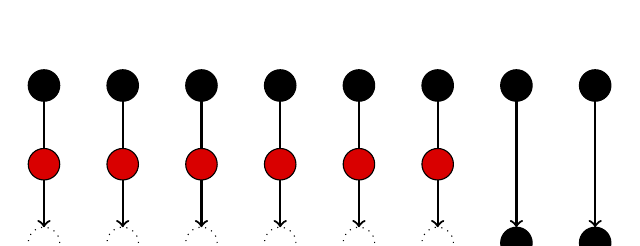
\begin{tikzpicture}
\foreach \x in {1,2,...,8} {
	\draw[fill] (\x,1) circle (0.2cm);
	\draw[->,thick] (\x,1) -- (\x,-0.8);
}
\foreach \x in {1,2,...,6} \draw[dotted] (\x,-1) circle (0.2cm);
\foreach \x in {1,2,...,6} \draw[fill=red!85!black] (\x,0) circle (0.2cm);
\draw[fill] (7,-1) circle (0.2cm);
\draw[fill] (8,-1) circle (0.2cm);
\end{tikzpicture}
\caption{Eight units of matter versus six units of antimatter!}
\label{fig:intadd}
\end{figure}
%\end{center}

We might visualize annihilation with a drawing like in \cref{fig:intadd} where black circles are units of matter, red circles are units of antimatter. Or, we could write a number sentence like $8 + \umin6 = 2$. Of course, no annihilations occur when we scrape together a big pile of matter (or a big pile of antimatter, for that matter). It's only when they mix that anything interesting happens.

\begin{boxeddef}[Adding Signed Numbers]
If the two numbers being added have the same sign, then we add the absolute values of the numbers, and use the sign that they share.

Otherwise, if the two numbers being added have different signs, then we find the difference between their absolute values, and use the sign of the number with larger absolute value.
\end{boxeddef}

\begin{boxedex}
Compute each of the following.

\begin{enumerate}[itemsep=10pt]
%\item \onerowex{$8+12$}{We add as usual, like we've been doing since elementary school: $8+12=20$}

\item \onerowex{$\umin8 + \umin12$}{Both numbers are negative. That's a big pile o' antimatter: $\umin8+\umin12 = \umin20$}

\item \onerowex{$\umin8 + 12$}{The numbers have different signs, so prepare for annihilation! $\abs{12}$ is larger than $\abs{\umin8}$, so we will have matter left over. Therefore, $\umin8 + 12 = 4$}

%\item \onerowex{$8 + \umin12$}{This time, we have more antimatter than matter: $8+\umin12 =\umin4$}
\end{enumerate}
\end{boxedex}

\subsection{Subtracting Signed Numbers}
\index{subtraction!of signed numbers}

Addition and subtraction are called \textit{opposite} (or \textit{inverse}) \textit{operations} because they ``undo'' one another. The act of adding 5 of matter can be ``undone'' by subtracting 5 units of matter. But on the other hand, the act of adding 5 units of matter can also be undone by \textit{adding 5 units of antimatter}.

\begin{boxeddef}[Subtracting Signed Numbers]
\textit{Subtracting a number} is the same as \textit{adding the opposite of the number}.

When faced with a subtraction problem, change it to an ``addition of the opposite'' problem and then follow the rules for adding signed numbers.
\end{boxeddef}

The benefit of this approach is that we can avoid having to learn a whole new set of rules for subtracting signed numbers. All we need are the rules for addition, plus one new rule about how to change subtraction problems into addition problems!

\begin{boxedex}
Compute each of the following:

\begin{enumerate}[itemsep=10pt]
\item \onerowex{$8-12$}{``Subtracting 12'' is the same as ``adding negative 12'', so $8-12=8+\umin12$. Then, we can apply the rules for adding signed numbers: $8+\umin12~=~\umin4$}

\item \onerowex{$\umin3 - 14$}{This is the same as $\umin3 + \umin14$, and we follow the rules for adding numbers with the same sign: $\umin3 + \umin14 = \umin17$}

\item \onerowex{$4 - \umin9$}{This is the same as $4 + 9$, which is an easy addition: $4+9=13$}

\item \onerowex{$\umin6 - \umin5$}{This is the same as $\umin6 + 5 = \umin1$}
\end{enumerate}
\end{boxedex}

When dealing with addition and subtraction of signed numbers in a problem, a good habit is to simplify the signs by rewriting subtraction as addition-of-the-opposite, before doing any computations.

\begin{boxedex}[Explaining the Startup Exploration]
In the startup exploration for this section, we have two natural numbers $x$ and $y$ where $x < y$. Natural numbers are all positive, so this means that $\abs{x}$ is less than $\abs{y}$.

Part (a) asks us to consider $x+(\umin y)$. Since opposite numbers have the same absolute value, $\abs{y}$ is the same as $\abs{\umin y}$. Therefore when we add, the number with larger absolute value is negative and the sum will take on the negative sign. So, when $x$ and $y$ are natural numbers and $x < y$, we know that $x+(\umin y)$ is \textit{always negative} so the result is always less than 0.

Part (b) asks us to consider $x-(\umin y)$. We can change this subtraction expression into addition-of-the-opposite: $x-(\umin y) = x+y$. Since both $x$ and $y$ are natural numbers, their sum is a natural number. In other words, when $x$ and $y$ are natural numbers, $x-(\umin y)$ is always positive, in other words always greater than 0.
\end{boxedex}

\subsection{Multiplying and Dividing Signed Numbers}
\index{multiplication!of signed numbers}
\index{division!of signed numbers}

Like addition and subtraction, the operations of multiplication and division are inverse operations. We'll discuss multiplication below, though the rules about the signs of products also apply to the signs of quotients.

Recall from your elementary school days that one way to think about whole number multiplication is as \textit{repeated addition}. We interpret $a \cdot b$ as ``$a$ groups with $b$ items in each group''. So, $3 \cdot 5$ means ``3 groups of 5'', which we can write as an addition sentence: $3 \cdot 5 = 5 + 5 + 5$.

Using this interpretation, we can easily explain the product of a positive number and a negative number. The expression $4\cdot\umin8$ means ``four groups of negative eight'': $4 \cdot \umin8 = \umin8 + \umin8 + \umin8 + \umin8 = \umin32$. No problem!

But what about $\umin5 \cdot 6$? What does it mean to have ``negative five groups of six''? Or even worse, what about $\umin3 \cdot \umin7$, ``negative three groups of negative seven''? Rather than try to twist the metaphor to fit these new situations, let's just admit that multiplication can not \textit{always} be represented by repeated addition.\footnote{The ``multiplication as repeated addition'' analogy breaks down when we have a negative number of groups, but also for rational and irrational numbers. What's the repeated addition problem for $\frac{2}{3} \cdot \frac{1}{2}$, or for $\sqrt{2} \cdot \sqrt{3}?$}

For the moment, we'll simply review the rules for multiplying (and dividing) signed numbers. We can explain why these rules work using the so-called ``field axioms for the real numbers''. More on that later.

\begin{boxeddef}[Multiplying (and Dividing) Signed Numbers]
The absolute value of the product of two numbers is the product of their absolute values: $\abs{a \cdot b} = \abs{a} \cdot \abs{b}$. If the two numbers have the same sign, then the product is positive. If the two numbers have opposite signs, then the product is negative.
\end{boxeddef}

There are several clever ways to remember this rule. Some people remember that every pair of negatives in a product cancel one another. Other people use a triangle with one positive sign and two negative signs drawn on the vertices. We present another way of looking at it in the next section. Choose whichever mnemonic\footnote{mnemonic ($na \cdot MON \cdot ic$, the first ``m'' is silent): A learning aid that helps to remember or retain information.} method is most helpful to you!

\subsubsection{Karmic Multiplication}

Karma, an underlying concept of many Eastern religions, is a belief that a person's actions and intentions shape their future. Performing good deeds will contribute to one's ``good karma'' and will lead to future happiness. Bad deeds contribute to one's ``bad karma'' and will lead to future suffering.

So, karma suggests that good things happen to good people, and that bad things happen to bad people. Of course we know that the universe does not always operate in accordance with karma.

\begin{boxeddef}[Karmic Multiplication]
\centering
When good things happen to good people, that's good!

When bad things happen to good people, that's bad!

When good things happen to bad people, that's bad!

When bad things happen to bad people, that's good!
\end{boxeddef}

For example: Mahatma Gandhi used nonviolent means to inspire civil rights movements around the world. Gandhi was a good person. On the other hand, Adolf Hitler was chancellor of Nazi Germany during World War II and orchestrated appalling crimes against humanity. Hitler was a bad person.\footnote{understatement ($UN \cdot der \cdot state \cdot ment$): The act of representing something in a weak or restrained way, to a lesser degree than is borne out by the facts.}

In terms of life events, winning the lottery is a good thing. Getting hit by a truck is a bad thing.

If Gandhi had won the lottery, that would have been in accordance with all his good karma. That's good! If Gandhi had been hit by a truck, that would have been in opposition to all of his good karma. That's bad!

If Hitler had won the lottery, that would have been in opposition to his evil karma. That's bad! If Hitler had been hit by a truck, it would have served him right! That's good! Go karma!

Of course, in this metaphor good things and good people represent positive numbers. Bad things and bad people represent negative numbers. When karma is operating as it should, we get a positive result. When the laws of karma are broken, we get a negative result.

\begin{boxedex}
Compute each of the following:

\begin{enumerate}[itemsep=10pt]
\item \onerowex{$8 \cdot \umin12$}{We multiply the absolute values and, since the two factors have different signs, we know the answer is negative: $8 \cdot \umin12 = \umin96$}

\item \onerowex{$\umin72 \div \umin3$}{We divide absolute values and, since the two factors have the same sign (both negative in this case, so that's ``Hitler gets his by a truck''), the answer is positive: $\umin72 \div \umin3 = 24$}
\end{enumerate}
\end{boxedex}

Note: When multiplying (or dividing) more than two numbers, we can approach things in two different ways. We might simplify the product two factors at a time, and keep track of the sign as we go. Or, we could treat the signs as a separate problem: first multiply all of the absolute values, then go back and count up the negative signs. %Suppose we count a total of 3 negative signs? Will our answer be positive or negative? What about if we could up 8 negative signs? Why?

\begin{boxedex}
Multiply: $(2)(\umin2)(1)(\umin2)(\umin2)(1)(1)(\umin2)(\umin1)(2)$

\exsoln{} If we count up the negative signs, we find there are five. Pairs of negatives will have a positive product, so we'll have two pairs of negatives plus one left over. Our final answer, then, will be negative. All that remains is to multiply the 2s (of which there are six): \[(2)(\umin2)(1)(\umin2)(\umin2)(1)(1)(\umin2)(\umin1)(2) = \umin64\]
\end{boxedex}

\begin{boxedex}[Explaining the Startup Exploration]
In the startup exploration for this section, $x$ and $y$ are natural numbers and $x<y$.

Since $x$ are $y$ are natural numbers they are both positive, and then $\umin y$ is negative. Part (c) asks us to consider $x\cdot(\umin y)$. We have a positive number times a negative number, so the product is \textit{always negative}, always less than 0.

Part (d) asks us to consider $x\div(\umin y)$. Again, we have a positive number and a negative number, so the quotient is \textit{always} less than 0.
\end{boxedex}


% % % % % % % % % % % % % % % % % % % % % % % % % % % % % % % % % % % % % % % % 
\section{Rational Numbers}
\label{sec:rationals}

As with integers, you've probably been working with fractions and decimals for a while now. In this section, we review the key terms and algorithms for working with rational numbers. As we get going, think about this:

\begin{boxedexplore}[Startup Exploration: Rational Comparisons]
In each of the expressions below, $a$ and $b$ are rational numbers where $0 < a < b < 1$. Will the result be greater than 1, less than 1, equal to 1, or is there not enough information to tell? Why?

a.\quad $a+b$
\hfill
b.\quad $a-b$
\hfill
c.\quad $a \cdot b$
\hfill
d.\quad $a \div b$
\hfill
\end{boxedexplore}

\subsection{The Language of Rational Numbers}

Sometimes in life we discover, much to our surprise, that some ridiculous and insignificant thing as been given a name.\footnote{For instance, did you know that the little plastic sheath at the end of your shoelaces is called an ``aglet''? Now you know.} We find ourselves wondering, ``Who decided to give \textit{that} a name? Why bother?'' Prepare for one of those moments:

\begin{boxeddef}[Vinculum]
A \gls{vinculum} (plural: vincula) is a horizontal bar used in mathematics to show grouping. For example, the fraction bar in the middle of $\frac{5}{2}$ is a vinculum.

Vincula are used in other contexts as well. For example, we use a vinculum to represent a repeating decimal such as $0.\overline{3}$.
\end{boxeddef}

With that definition in mind, we can continue with two of the most daunting words in elementary mathematics. You're definitely not alone if you have ever been confused about these.

\begin{boxeddef}[Numerator and Denominator]
In a fraction, the number above the vinculum is called the \gls{numerator} of the fraction, and the number below the vinculum is called the \gls{denominator} of the fraction.

For example in the number $\frac{5}{6}$, the numerator is 5 and the denominator is 6.
\end{boxeddef}

%%% minipage to have fraction image inline with text
\bigskip
\begin{minipage}{0.66\textwidth}
If we ask ``\textit{how many} sixths?'', the numerator tells us ``\textit{five} sixths''. The word numerator is related to the word ``number'', and the numerator counts the pieces.

If we ask ``five \textit{whats}?", the denominator tells us ``five \textit{sixths}''. The word denominator is related to the word ``nominate'' (as in ``to nominate someone for president'') which means ``to name''. The denominator \textit{names} the fraction.
\end{minipage}
%
\begin{minipage}{0.33\textwidth}
	\begin{center}
	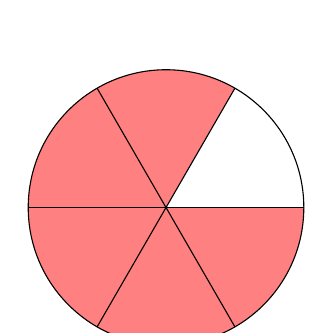
\begin{tikzpicture}[scale=1.75]
		\fill[red!50] (0,0) circle[radius = 1cm];
		\fill[white] (0,0) -- (1cm,0cm) arc (0:60:1cm) -- (0,0);
		\draw (0,0) circle[radius = 1cm];
		\foreach \t in {0,60,120} \draw[rotate=\t] (-1,0) -- (1,0);
	\end{tikzpicture}
	\end{center}
\end{minipage}

\subsection{Multiplying Rational Numbers}
\index{multiplication!of rational numbers}

Don't worry, your version of the \algebranomicon{} isn't missing any sections. Most textbooks would discuss adding and subtracting rational numbers, but we're going to start by studying the most helpful of the rational number operations: multiplication.

Suppose that at the cheese market, Knut Krumbli is selling chunks from a 10-pound block of cave-aged goat cheese.\footnote{When cheese is aged in the cool, humid air of underground caves, it can develop a denser texture and a more complex flavor, since small salt crystals form throughout its interior.} Half of the original block of cheese is left, and a local weaver asks to buy three-fourths of it. The original block had a value of 800 Swedish kronor. How much should Knut charge the weaver?

Let's draw a picture (\cref{fig:fracmult}). In the images below, the square represents the original block of cheese. We divide the square in half vertically, and the region shaded yellow represents how much of the cheese remains. We can then divide the cheese into fourths horizontally and shade in three-fourths (the amount that the weaver wants to buy) in blue.

\begin{figure}[!htbp]
\centering
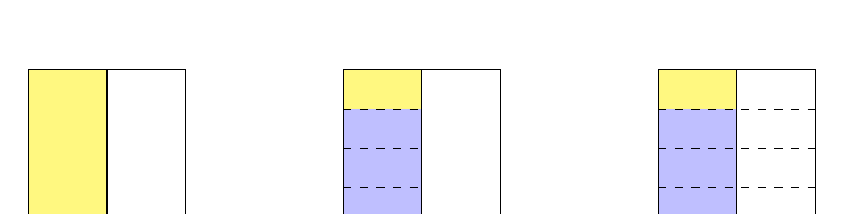
\begin{tikzpicture}
	\draw[fill=yellow!50] (0,0) rectangle (1,2);
	\draw(0,0) rectangle (2,2);

	\draw[fill=yellow!50] (4,0) rectangle (5,2);
	\fill[blue!25] (4,0) rectangle (5,1.5);
	\draw(5,0)--(5,2);
	\draw[dashed] (4,0.5) -- (5,0.5);
	\draw[dashed] (4,1) -- (5,1);
	\draw[dashed] (4,1.5) -- (5,1.5);
	\draw(4,0) rectangle (6,2);

	\draw[fill=yellow!50] (8,0) rectangle (9,2);
	\fill[blue!25] (8,0) rectangle (9,1.5);
	\draw(9,0)--(9,2);
	\draw[dashed] (8,0.5) -- (10,0.5);
	\draw[dashed] (8,1) -- (10,1);
	\draw[dashed] (8,1.5) -- (10,1.5);
	\draw(8,0) rectangle (10,2);
\end{tikzpicture}
\caption{Selling three-fourths of one-half of a block of cheese.}
\label{fig:fracmult}
\end{figure}

What fraction of the whole block does this blue region represent? If we extend the lines, we can see that we've divided up the whole block of cheese into 8 equally-sized pieces. So the weaver is buying $\frac{3}{8}$ of the whole block and Knut should charge 300 kronor.

In the end, we solved a fraction multiplication problem: ``How much is three-fourths of one-half of a whole block of cheese?'' \[\frac{3}{4} \cdot \frac{1}{2} = \frac{3}{8}\] 

\begin{boxeddef}[Multiplying Rational Numbers]
To multiply rational numbers, we multiply numerators to find the numerator of the product. We multiply denominators to find the denominator of the product. \[\frac{a}{b} \cdot \frac{c}{d} = \frac{a \cdot c}{b \cdot d}\]
\end{boxeddef}

\begin{boxedex}[Explaining the Startup Exploration]
In the startup exploration for this section, $0 < a < b < 1$, and part (c) asks us to consider $a \cdot b$. Let's think about this from a block-of-cheese perspective. We start with less than a whole block of cheese (since $b$ is less than 1) and we only want to buy a fraction of what's there (since $a$ is less than 1).

So, we are certainly buying less than a whole block of cheese! Since both $a$ and $b$ are less than 1, we know that their product must be less than one.
\end{boxedex}

\subsubsection*{Fancy Versions of One}

Recall that any number times 1 is itself. This simple fact, along with the fraction multiplication procedure, gives us an extremely powerful tool that we'll use in various different ways throughout algebra. The key idea is that multiplying something by 1 doesn't change its value, even if we use a ``fancy version of 1''.\footnote{Multiplication by a fancy version of 1 is an application of the identity property of multiplication, which we will study in more detail in \cref{ch:equations}.} Consider, for example:
\[\begin{aligned}
\frac{5}{8} &= \frac{5}{8} \cdot 1
&& \quad\text{Multiplication by 1 doesn't change the number.}
\\
\\
&= \frac{5}{8} \cdot \frac{7}{7}
&& \quad\text{We can rewrite 1 however we like, here $1 = \frac{7}{7}$.}
\\
\\
&= \frac{35}{56}
&& \quad\text{Multiply fractions.}
\end{aligned}\]
In the end, we have two equivalent fractions $\frac{5}{8} = \frac{35}{56}$. The representation has changed, but the value is the same! The ``fancy one'' we chose here is $\frac{7}{7}$, but any other version of 1 would work the same way: $\frac{-140}{-140}$, $\frac{2\pi}{2\pi}$, $\frac{\sqrt3}{\sqrt3}$\ldots{} The possibilities are endless.

The first application of the ``fancy one'' has to do with one of the themes we encounter throughout algebra: the idea of finding a ``completely simplified'' solution to a problem. Fractions introduce us to the first criteria for something being simplified.

\begin{boxedcriteria}[Simplified Rational Numbers \#1]
Fractions should be simplified to \gls{lowest terms}, meaning that the numerator and denominator of the fraction are \gls{relatively prime} integers.
\end{boxedcriteria}

Two integers are said to be relatively prime (or coprime) if they have no common factors other than 1. So, the fraction $\frac{21}{34}$ is in lowest terms, since the factors of 21 are $\{1, 3, 7, 21\}$ and the factors of 34 are $\{1, 2, 17, 34\}$. They have no factors in common, other than 1.

On the other hand, $\frac{18}{84}$ is not in lowest terms. Both 18 and 84 are even, and so both the numerator and denominator are divisible by at least 2. To write this fraction in lowest terms, we ``undo'' fraction multiplication and search for some fancy ones that we can eliminate: \[\frac{18}{84} = \frac{2 \cdot 3 \cdot 3}{2 \cdot 2 \cdot 3 \cdot 7}  = \frac{2}{2}\cdot\frac{3}{3}\cdot\frac{3}{2\cdot 7} = 1\cdot1\cdot\frac{3}{14} = \frac{3}{14}\]
Once we know how and why this works, we can take a shortcut and ``cancel'' common factors from the numerator and denominator: \[\frac{18}{84} = \frac{2 \cdot 3 \cdot 3}{2 \cdot 2 \cdot 3 \cdot 7}=\frac{\bcancel{2} \cdot \cancel{3} \cdot 3}{\bcancel{2} \cdot 2 \cdot \cancel{3} \cdot 7}  = \frac{3}{2 \cdot 7}\]

\subsubsection*{Simplify Before You Multiply}

We can also use the ``fancy one'' to save ourselves some work! What if we have to multiply:
\[\frac{1}{2} \cdot \frac{2}{3} \cdot \frac{3}{4} \cdot \frac{4}{5} \cdot \frac{5}{6}\]
Let's write the product out ``the long way'' before we actually do any computations. The numerator of the product will be the product of the numerators, and likewise for the denominator:
\[\frac{1}{2} \cdot \frac{2}{3} \cdot \frac{3}{4} \cdot \frac{4}{5} \cdot \frac{5}{6} = \frac{1 \cdot 2 \cdot 3 \cdot 4 \cdot 5}{2 \cdot 3 \cdot 4 \cdot 5 \cdot 6}\]
Then, a common factor in the numerator and denominator is like multiplication by 1, so we can make some simplifications:
\[\frac{1}{2} \cdot \frac{2}{3} \cdot \frac{3}{4} \cdot \frac{4}{5} \cdot \frac{5}{6} = \frac{1 \cdot 2 \cdot 3 \cdot 4 \cdot 5}{2 \cdot 3 \cdot 4 \cdot 5 \cdot 6} = \frac{1 \cdot \cancel{2} \cdot \bcancel{3} \cdot \cancel{4} \cdot \bcancel{5}}{\cancel{2} \cdot \bcancel{3} \cdot \cancel{4} \cdot \bcancel{5} \cdot 6} = \frac{1}{6}\]
The alternative would have been to multiply all of those numbers together by hand and then simplify the fraction to lowest terms\footnote{That would have been $\frac{120}{720}$.}, which is a bunch more work. It pays to be clever!

\begin{boxedex}
Multiply: (a)~ $\dfrac{3}{4} \cdot \dfrac{7}{16}$ \quad (b)~ $\dfrac{15}{8}\cdot\dfrac{4}{7}\cdot\dfrac{14}{3}\cdot\dfrac{1}{5}$

Problem (a) is nothing special. No common factors are shared between numerators and denominators, so we simply multiply as usual.\[\frac{3}{4} \cdot \frac{7}{16} = \frac{3 \cdot 7}{4 \cdot 16} = \frac{21}{64}\] Since there were no common factors to cancel before multiplying, we know the product is already in lowest terms.

To tackle (b), the first helpful step is to factor the individual numerators and denominators to expose all of the factors that are going to be in the product. \[\frac{3\cdot 5}{2 \cdot 2 \cdot 2} \cdot \frac{2 \cdot 2}{7} \cdot \frac{2 \cdot 7}{3} \cdot \frac{1}{5}\]
Then, a common factor in the numerator and denominator is like multiplication by 1, so common factors can be crossed out. Look at what happens in this case!
\[\frac{\cancel{3}\cdot \cancel{5}}{\bcancel{2} \cdot \bcancel{2} \cdot \bcancel{2}} \cdot \frac{\bcancel{2} \cdot \bcancel{2}}{\bcancel{7}} \cdot \frac{\bcancel{2} \cdot \bcancel{7}}{\cancel{3}} \cdot \frac{1}{\cancel{5}} = 1\]
Note that all of the factors cancel out in the denominator. A common mistake at this point is to replace the ``empty'' denominator with 0 -- but remember, a common factor in the numerator and denominator is like a factor of 1, which is the fraction $\frac{1}{1}$, not $\frac{1}{0}$, so there's always a ``phantom one'' lurking there even if we don't write it.
\end{boxedex}

\subsection{Adding and Subtracting Rational Numbers}
\index{addition!of rational numbers}
\index{subtraction!of rational numbers}

Knut Krumbli would tell you that brining together a herd of 8 goats and a herd of 11 goats results in a herd of 19 goats. It's goat herding, not rocket science.

But, combining a herd of 4 goats and a flock of 13 sheep doesn't really give us 17 of anything until we can find some shared characteristic that is common to both groups. For instance, we could say we have a group of ``17 mammals'', or ``17 quadrupeds''.

So it goes with fractions. When our fractions have a shared name (a common denominator) we can total up how many things we have with that name: 8 thirds and 11 thirds makes 19 thirds. In math symbols, we write \[\frac{8}{3} + \frac{11}{3} = \frac{19}{3}\] When our quantities \textit{don't} share a common unit (a common denominator), we have to find one before we can add in a meaningful way.

Given a fraction, we can use multiplication by a ``fancy one'' to generate a new fraction that has the same value but a different, perhaps more helpful, denominator.

Some people like to try and find the \textit{least common denominator}, but that's not strictly necessary. Any common denominator will do. In fact, a guaranteed common denominator of any two fractions is the \textit{product of their denominators}.

\begin{boxeddef}[Adding and Subtracting Rational Numbers]
To add rational numbers, we must have a common denominator, for example the product of the original denominators. Then we add the numerators, and keep the common denominator.
\[\frac{a}{b} + \frac{c}{d}
= \frac{a\cdot d + b\cdot c}{b\cdot d}\]
To subtract rational numbers, change the subtraction problem to an ``addition of the opposite'' problem and then follow the algorithm for addition.

Here's the derivation of fraction addition in a bit more detail. Note how we use multiplication by 1 to find a common denominator $b \cdot d$:
\[\frac{a}{b} + \frac{c}{d}
= \left( \frac{a}{b}\cdot 1 \right) + \left( 1\cdot\frac{c}{d} \right)
= \left( \frac{a}{b}\cdot\frac{d}{d} \right) + \left( \frac{b}{b}\cdot\frac{c}{d} \right)
= \frac{a\cdot d}{b\cdot d} + \frac{b\cdot c}{b\cdot d}
= \frac{a\cdot d + b\cdot c}{b\cdot d}\]

\end{boxeddef}

\subsubsection*{Negative Fractions}

Where should we put the negative sign when we have a negative fraction? Does it matter? Consider the following three possibilities. Are they all equivalent? \[ -\frac{3}{4} = \frac{-3}{4} = \frac{3}{-4}\]
A fraction is a way of writing a division problem. If Knut's four children share three bowls of lingonberries equally, then each child will get $3\div4 = \frac{3}{4}$ of a bowl of berries.\footnote{Lingonberries are a popular fruit in Scandinavia and throughout northern, central, and eastern Europe. The berries are quite tart, and so they are usually mixed with sugar and preserved as jam or compote. In Sweden and Norway, reindeer is traditionally served with gravy and lingonberry sauce. Yes, Scandinavians eat reindeer.} The fraction $\frac{3}{4}$ is just another way of writing $3 \div 4$.

So, all three of the fractions above have the same value. In the first example, the whole fraction has been negated. In the second and third examples, the numbers have opposite signs and so the quotient will be negative. In other words it actually doesn't matter where we put the negative sign. We can put it where it is most convenient for the problem (very often, that's in the numerator of the fraction).

\subsubsection*{Mixed Numbers}

Improper fractions have a numerator that is greater than or equal (in absolute value) to their denominator, like $\frac{5}{3}$ or $\frac{-84}{16}$. Improper fractions have been scorned by many elementary school mathematics teachers, who instead prefer mixed numbers: $1\frac{2}{3}$ or $-5\frac{1}{4}$. But, improper fractions are often much easier to work with than mixed numbers.\footnote{One situation where improper fractions are superior is when describing the slope of a line, as we will see in \cref{ch:linear}.}

\begin{boxedcriteria}[Simplified Rational Numbers \#2]
Simplified \glspl{improper fraction} are preferred over \glspl{mixed number} and decimals. Only convert to a mixed number or decimal when the context (or the directions) require it.
\end{boxedcriteria}

We usually prefer exact fraction answers over decimal approximations. Writing the decimal $\frac{10}{7}$, for instance, is much preferred over $1.43$, and better even than the exact answer $1.\overline{428571}$ (yep, that's a big chuck o' repeating decimal).

But, be sure to read questions carefully! There are exceptions to these rules. When working in a real-world context, a certain number format may make more sense. For example, when solving a problem about money, the answer \$3.50 makes a lot more sense than $\$\frac{7}{2}$. Likewise, the answer ``$1\frac{1}{3}$~pounds of cheese'' is better than ``$\frac{4}{3}$~pounds of cheese''. In ambiguous cases, we will make it clear what number format is preferred.

When faced with mixed numbers in a problem, we have to be careful. When adding, we can convert all mixed numbers to improper fractions, or work with them ``as is''. Subtracting with mixed numbers is tricky, however, because we we may have to handle regrouping. Multiplication is even trickier.

Since we prefer improper fractions as final answers anyway, we recommend converting all mixed numbers to improper fractions before you start computations. To convert a mixed number to an improper fraction, all we have to do is think about the mixed number as an addition problem:
\[3\frac{5}{8} = 3 + \frac{5}{8} = \frac{3}{1} + \frac{5}{8} = \frac{3 \cdot 8 + 1 \cdot 5}{1 \cdot 8} = \frac{24 + 5}{8} = \frac{29}{8}\]
Here we used the fact that any integer has a ``phantom one'' in its denominator: $3 = \frac{3}{1}$. We don't usually write it, but it's there when we need it.

\begin{boxedex}
Compute each of the following:

\begin{enumerate}[itemsep=10pt]
\item \onerowex{$\dfrac{3}{4} + \dfrac{5}{6}$}{These fractions do not have a common denominator, so we'll have to find one. We could use their least common denominator (which is 12) or use the product of the denominators (which is 24). Let's use 24: \[\dfrac{3}{4} + \dfrac{5}{6} = \dfrac{3 \cdot 6 + 4 \cdot 5}{4 \cdot 6} = \dfrac{18 + 20}{24} = \dfrac{38}{24} = \dfrac{19}{12}\]}

\item \onerowex{$1\dfrac{2}{5} - 1\dfrac{7}{8}$}{First, we'll convert to improper fractions and change the subtraction to addition-of-the-opposite, putting the negative sign in the numerator of the fraction. Then we add. In the end, we can adjust the negative sign again: \[\dfrac{7}{5} - \dfrac{15}{8} = \dfrac{7}{5} + \dfrac{\umin15}{8} = \dfrac{7 \cdot 8 + 5 \cdot \umin15}{5 \cdot 8} = \dfrac{56 + \umin75}{40} = \dfrac{\umin19}{40} = -\dfrac{19}{40}\]}
\end{enumerate}
\end{boxedex}

\begin{boxedex}[Explaining the Startup Exploration]
In the startup exploration for this section, $0 < a < b < 1$.

Part (a) asks about $a + b$. Since both numbers are positive, their sum is positive, but we don't have enough information to tell whether the sum is greater than 1. If $a$ and $b$ are both less than $\frac{1}{2}$, for example, then their sum will be less than 1. On the other hand, if they are both greater than $\frac{1}{2}$, then their sum will be greater than 1.

Part (b) asks us to consider $a - b$. Since $a$ is less than $b$, we're subtracting a larger number from a smaller number, and so the answer must be negative.

We can reason this out in another way: $a-b$ is the same as $a + (\umin b)$. The absolute value of $b$ is the same as the absolute value of $\umin b$. And so this sum will be negative because the negative number is the one with the greater absolute value.

In any case, $a-b$ is negative and so we know for sure that it is less than 1.
\end{boxedex}

\subsection{Dividing Rational Numbers}
\index{division!of rational numbers}

Fraction division may be the most poorly understood operation in all of arithmetic. The algorithm for dividing fractions seems arbitrary, and it's often difficult to judge whether our answers make sense. Let's pause for a moment to think about what fraction division means.

Suppose Jorunn Krumbli, Knut's wife, is making scarves for the goats (Scandinavian winters are chilly). She has 8 meters of burlap, and each scarf requires $\frac{3}{4}$ of a meter. How many scarves can she make?

This question is asking us to compute $8 \div \frac{3}{4}$, but let's try to solve the problem by drawing a picture. Suppose this rectangle represents Jorunn's 8 meters of burlap.
\begin{center}
\begin{tikzpicture}
	\foreach \x in {0,2,...,14} \draw (\x,0) rectangle (\x+2,1);
\end{tikzpicture}
\end{center}

To figure out how many pieces of $\frac{3}{4}$ meter are in there, let's first determine the number of pieces of size $\frac{1}{4}$ meter. To do that, we'll break each meter into four pieces. That gives us $8 \cdot 4 = 32$ pieces total.
\begin{center}
\begin{tikzpicture}
	\foreach \x in {0,0.5,...,15.5} \draw[blue,dashed] (\x,0) -- (\x,1);
	\foreach \x in {0,2,...,14} \draw (\x,0) rectangle (\x+2,1);
\end{tikzpicture}
\end{center}

Now, let's gather these pieces up into groups of three. We'll be able to make 10 whole groups, and we'll have 2 pieces left over. Since we have two pieces, but need three, we have $\frac{2}{3}$ of a group. So, Jorunn can make $10\frac{2}{3}$ scarves for the goats.
\begin{center}
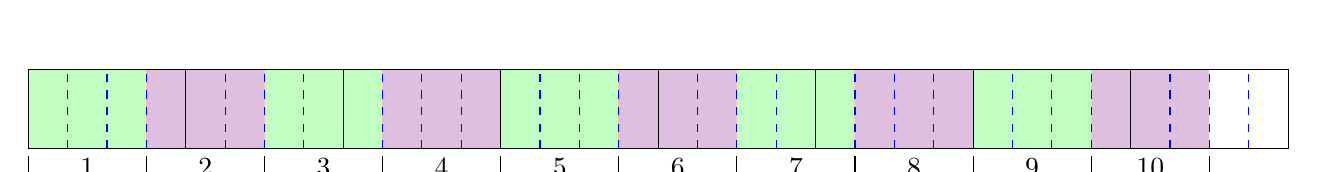
\begin{tikzpicture}
	\foreach \x in {1.5,4.5,...,13.5} \draw[white,fill=violet!25] (\x,0) rectangle (\x+1.5,1);
	\foreach \x in {0,3,...,12} \draw[red!25,fill=green!25] (\x,0) rectangle (\x+1.5,1);
	\foreach \x in {1,...,10} {
		\draw (1.5*\x-1.5, -.1) -- (1.5*\x-1.5, -.3);
		\draw (15, -.1) -- (15, -.3);
		\draw (1.5*\x-0.75,0) node[below]{\x};
	}
	\foreach \x in {0,0.5,...,15.5} \draw[blue,dashed] (\x,0) -- (\x,1);
	\foreach \x in {0,2,...,14} \draw (\x,0) rectangle (\x+2,1);
\end{tikzpicture}
\end{center}

Let's retrace our steps. We set out to solve $8 \div \frac{3}{4}$, but in our picture we first multiplied to find the total number of fourths, and then we divided to find how many groups of three we could make. In other words: $8 \div \frac{3}{4}$ must have the same answer as $8 \cdot \frac{4}{3}$. Does that look familiar?

\begin{boxeddef}[Dividing Rational Numbers]
Dividing by a number is the same as multiplying by the reciprocal of the number. So, we can change a given fraction division problem into an equivalent fraction multiplication problem and then use the rules for fraction multiplication. \[\frac{a}{b} \div \frac{c}{d} = \frac{a}{b} \cdot \frac{d}{c} = \frac{a \cdot d}{b \cdot c}\]
\end{boxeddef}

Recall that the \gls{reciprocal} of a fraction is the fraction that interchanges the numerator and the denominator of the original fraction. The reciprocal of an integer (which is sitting on a phantom 1) is ``one over the original integer''.

\begin{boxedex}
Compute each of the following:

\begin{enumerate}[itemsep=10pt]
\item \onerowex{$\dfrac{5}{6} \div -\dfrac{3}{4}$}{We don't need a common denominator or anything, so we can just jump right in with fraction division. We don't even need to move the negative sign, since we know the answer will be negative. \[\dfrac{5}{6} \div -\dfrac{3}{4} = \dfrac{5}{6} \cdot -\dfrac{4}{3} = -\dfrac{20}{18} = -\dfrac{10}{9}\]}

\item \onerowex{$3\dfrac{3}{4} \div 5$}{First, we'll convert to improper fractions, then we'll implement fraction division At the end, we can simplify before we multiply! \[3\dfrac{3}{4} \div 5 = \dfrac{15}{4} \div \dfrac{5}{1} = \dfrac{15}{4} \cdot \dfrac{1}{5} = \dfrac{3 \cdot 5}{4} \cdot \dfrac{1}{5} = \dfrac{3 \cdot \cancel{5}}{4} \cdot \dfrac{1}{\cancel{5}} = \dfrac{3}{4}\]}
\end{enumerate}
Let's think about this last answer for a second: does it makes sense? Look again at the problem we were given. If we interpret this as the question``how many groups of 5 are in $3\frac{3}{4}$?'', then we can see that we can't even make one whole group: $3\frac{3}{4}$ is less than 5! So, it makes sense for our answer to be less than 1.
\end{boxedex}

\subsubsection*{Fractions Inside Fractions}

As if fractions on their own weren't enough, you may soon face the turducken\footnote{A ``turducken'' is a food product where a deboned chicken is stuffed inside a deboned duck, which is then stuffed inside a deboned turkey. In culinary terminology, this is an example of ``engastration'', a cooking method in which one animal is stuffed inside the gastric cavity of another\ldots{} which is probably yet another phenomenon that you didn't know had a name.} of arithmetic, the dreaded ``fraction in a fraction''. Note that the first criteria for simplified rational numbers states that the numerator and denominator must be \textit{integers}.

These creatures can look hard to handle, but don't be intimidated. Recall that a fraction is just a division problem. So, we can rewrite things using a division sign and divide as usual.\footnote{The fancy mathematical name for the $\div$ symbol is \textit{obelus} (plural: obeli)\ldots{} another thing that you probably didn't know had a name).}

\begin{boxedex}
Simplify each of the following:

\begin{enumerate}[itemsep=10pt]
\item \onerowex{$\dfrac{~~4~~}{\left( \frac{1}{3} \right)}$}{All we have to do is rewrite the fraction-in-a-fraction as ``numerator $\div$ denominator'', and then divide as usual. \[\dfrac{~~4~~}{\left( \frac{1}{3} \right)} = 4 \div \dfrac{1}{3} = 4 \cdot \dfrac{3}{1} = 4 \cdot 3 = 12\]}

\item \onerowex{$\dfrac{~~\left( \frac{2}{5} \right)~~}{\left( 1\frac{3}{8} \right)}$}{Here we must rewrite using the obelus, then convert to improper fractions, then divide! \[\dfrac{~~\left( \frac{2}{5} \right)~~}{\left( 1\frac{3}{8} \right)} = \dfrac{2}{5} \div 1\dfrac{3}{8} = \dfrac{2}{5} \div \dfrac{11}{8} =\dfrac{2}{5} \cdot \dfrac{8}{11} = \dfrac{16}{55}\]}
\end{enumerate}
\end{boxedex}

\begin{boxedex}[Explaining the Startup Exploration]
In the startup exploration for this section, we have rational numbers $a$ and $b$ where $0 < a < b < 1$. Part (d) asks us to consider $a \div b$. This division problem is another way of writing $\frac{a}{b}$. Since $a$ is less than $b$, though, we know that this fraction is a proper fraction (as opposed to an improper fraction), which means it is less than 1. So, $a \div b$ is less than 1.
\end{boxedex}

\subsection{Evil and Wrong}

Everyone makes mistakes, but not all mistakes are created equal. Some mistakes are not just wrong, the are \evilandwrong. ``Wrong'' because they are mistakes, ``evil'' because they are subtle, and sneaky, and tempting.

What we mean here is that sometimes we feel drawn to perform certain arithmetic or algebraic maneuvers -- some things seem so logical, so easy, so natural, so tempting -- when in reality, they are a total trap. For example:

\begin{boxedwarning}
Armed with the idea of ``simplify before you multiply'', we might want to try and pull this stunt in other places: \[\frac{2+3}{2+7} = \frac{\bcancel{2}+3}{\bcancel{2}+7} = \frac{3}{7}\]Seems logical, right? But so wrong! There is no ``simplify before you add'' maneuver, tempting though it may be. Such a thing is \evilandwrong.
\end{boxedwarning}

You may be thinking, ``Nah, I'd never to that,'' and with numerical expressions like these, you may be right. But later, when faced with variable expressions like \[\frac{x+3}{x+7}\]
this temptation may come back, in disguise. We'll draw attention to these \evilandwrong{} mistakes as we go along because they are so tempting. Beware!


% % % % % % % % % % % % % % % % % % % % % % % % % % % % % % % % % % % % % % % % 
\section{Order of Operations}
\label{sec:orderofops}

We turn now to something else that it probably familiar, the \gls{order of operations}. Consider the following problem as we get started:

\begin{boxedexplore}[Startup Exploration: Who's Right?]
The four Krumbli kids each performed the following computation: \[14 - 6 \cdot 7 + 10\] Sini got $\umin38$,
Siri got $\umin18$,
Sten got $66$,
and Stig got $136$. Which of them performed the computation correctly? What mistakes did the others make?
\end{boxedexplore}

The order of operations gives us a standard procedure for simplifying numeric expressions. A \gls{numeric expression} is the algebra way of describing something you may have called just a ``math problem'' in elementary school. For example $12 - 5$ is a numeric expression. It is not in its simplest form because we can evaluate $12 - 5$ and write 7 instead.  

\begin{boxedcriteria}[Simplification Rule \#1]
A numeric expression is completely simplified if all operations have been evaluated and all grouping symbols have been eliminated. The resulting quantity is called the \textit{value} of the expression.
\end{boxedcriteria}

As we go along in algebra, we will learn many rules that maintain ``mathematical equivalence.''  Expressions are mathematically equivalent if they represent the same quantity.  For example, $\frac{4}{8}$ is equivalent to $\frac{1}{2}$, and $12 - 5$ is equivalent to 7. Our job when we simplify is to maintain the equivalence from one step to the next. The order of operations is a set of rules for how to do that.

\begin{boxeddef}[Order of Operations]
The \gls{order of operations} is an agreed-upon order for simplifying numeric expressions. The big idea is that ``more powerful'' operations take priority over ``less powerful'' operations. When we want to alter the usual rules of precedence, we introduce grouping symbols to make our intentions clear.

When simplifying an expression, we evaluate things in the following order:\footnote{PEMDAS is an mnemonic acronym for remembering the order of operations: Parentheses, Exponents, Multiplication, Division, Addition, Subtraction. In Canada it's BEDMAS (B for Brackets). In the UK and Australia it's BIDMAS or BODMAS (Indices or Orders, which are other words for exponent). A better acronym might be GEMS or PEMA, which group together the pairs of operations that have the same priority (the G is for Grouping symbols).}

\begin{description}
\item[First:] Grouping symbols like (parentheses), [square brackets], \{curly braces\}, as well as other subtle grouping symbols like absolute value and the vinculum. Here we work from the innermost set of groupers\footnote{As in grouping symbols, not the fish.} to the outermost.

\item[Then:] Exponents (and, later, roots and logarithms). In the case of a ``stack'' of exponents, work from the top down.

\item[Then:] Multiplication and division. Recall that dividing is the same as ``multiplying by the reciprocal''. So, these two operations have the same priority and we work from left to right.

\item[Finally:] Addition and subtraction. Recall that ``subtracting'' is the same as ``adding the opposite''. So, these two operations have the same priority and we work from left to right.
\end{description}
\end{boxeddef}

\begin{boxedex}[Explaining the Startup Exploration]
Simplify: $14 - 6 \cdot 7 + 10$

\exsoln{} The correct answer follows the order of operations, like so
\[\begin{aligned}
	&~ 14 - 6 \cdot 7 + 10\\
=	&~ 14 - 42 + 10
&& \quad\text{work multiplication before addition/subtraction}\\
=	&~ \umin28 + 10
&& \quad\text{work addition and subtraction from left to right}\\
=	&~ \umin18
\end{aligned}\]
So, it is Siri who had the right answer.

Students who just memorize a clever mnemonic device might be tempted to do the \underline{A}ddition before the \underline{S}ubtraction, but don't be fooled! Those two operations have the same priority. (Sini made this mistake and got $\umin38$.)

Sten worked the operations straight through from left to right, all at the same priority and got 66. Stig did something very creative, computing $(14-6)\cdot(7+10) = 8 \cdot 17 = 136$.
\end{boxedex}

Notice how we showed the work going down the page, simplifying the problem one step at a time. Some people prefer to work across, and that's OK too. The point is that it's important to show work in an organized way when we solve a problem so that our reasoning and thought process are clear.

%\addtodoitem{Criteria for showing work.}

The work you show is the road map to your solution. Whoever reads over your work must be able to follow and understand your steps, without having to make any assumptions about what you actually did to reach your answer. It's a bad habit to skip steps, and it's no help to people reading your work to say you did a step in your head. Every step you take needs to be written down clearly and neatly.

\begin{boxedwarning}[Abuse of the Equal Sign]
Consider the following work, written out by a student to simplify $8 \cdot 4 + 10$ \[8 \cdot 4 = 32 + 10 = 42 \qquad\text{OK or not OK?}\]
The student has reached the correct value, and it may even be clear what the student is thinking: ``8 times 4 is 32, plus 10 more makes 42''. This, however, is a heinous abuse of the equal sign! Look at what the first part of the work says: \[8 \cdot 4 = 32 + 10 \qquad\text{These are not equal!}\]
One way to avoid this misuse of the equal sign is to write your work going down the page (as shown above). If you prefer to write across the page, be sure to write out the whole problem as you perform each simplification: \[8 \cdot 4 + 10 = 32 + 10 = 42\]
\end{boxedwarning}

In the next few sections, we'll look more closely at some trickier aspects of the order of operations.

\subsection{About Grouping Symbols}

As expressions get complicated, we may have grouping symbols inside of other grouping symbols. If there are different symbols, we can more easily see where different groups begin and end. But, we may just find a bunch of parentheses, like in the example below. In that case, we have to be a bit careful about what's being grouped together.

\begin{boxedex}
Simplify: $12+(3-(4-2)+5)$

\exsoln{} When faced with multiple grouping symbols, we must start with the innermost set of grouping symbols and evaluate our way to the outermost. Once we have simplified the expression inside a set of grouping symbols down to a single quantity, we can write that quantity without the groupers.
\[\begin{aligned}
	&~ 12+(3-(4-2)+5)\\
=	&~ 12+(3-2+5)\\
=	&~ 12+(1+5)\\
=	&~ 12+6\\
=	&~ 18
\end{aligned}\]
\end{boxedex}

\subsubsection{The Vinculum Is a Grouping Symbol}

The \gls{vinculum} (as in the fraction bar) is a grouping symbol. For example, if the task is to simplify a fraction such as: \[\frac{20+2^2\cdot(14-9)}{(2-4)^3}\] then we must think of the expression in the numerator as a group, and likewise for the denominator. In other words, like so: \[\Bigl(20+2^2\cdot(14-9)\Bigr)\div\Bigl((2-4)^3\Bigr)\]

We have two options for simplifying this. We might keep it in a fraction the whole time, or we could simplify the numerator and denominator separately and then squish them back into a fraction at the end.

\begin{boxedex}
Simplify: $\dfrac{20+2^2\cdot(14-9)}{(2-4)^3}$

\exsoln{} Let's dismantle this thing and handle it in two pieces. The numerator works like this:
\[\begin{aligned}
	&~ 20 + 2^2 \cdot (14-9)\\
=	&~ 20 + 2^2 \cdot 5\\
=	&~ 20 + 4 \cdot 5\\
=	&~ 20 + 20\\
=	&~ 40
\end{aligned}\]
The denominator works like this: $(2-4)^3 = (\umin2)^3 = \umin8$. Then, we can put the pieces back into their original fraction configuration:\[\dfrac{20+2^2\cdot(14-9)}{(2-4)^3} = \dfrac{40}{\umin8} = \umin5\]
\end{boxedex}

\subsection{About Exponents}

An expression of the form $a^b$ is read ``$a$ to the power of $b$'' or ``$a$ to the $b^{\text{th}}$ power''. In such an expression, $a$ is called the \gls{base} and $b$ is called the \gls{exponent}. We call the whole thing a \gls{power} of $a$, since $a$ is the base.

We will get into more detail about exponents later on, but we'll pause here to mention two key ideas. First, recall that we can think about an exponent as shorthand for a repeated multiplication.\footnote{As with ``multiplication is repeated addition'', this interpretation breaks down eventually. Expressions like $5^{-3}$ and $16^{\frac{1}{2}}$ don't really translate well into ``repeated multiplication''. Don't panic about the idea of a negative number or a fraction up there in the exponent! All will be revealed as the course goes on.}
\[a^b = \underbrace{a \cdot a \cdot a \dotsb a}_{\text{$b$ times}}\]
That part you probably knew already. This next fact may be new.

\begin{boxeddef}[Raising to the Power Zero]
For any nonzero number $a$, the expression $a^0 = 1$. In other words, any nonzero number raised to the power 0 equals 1.

When we say that $a$ is a ``nonzero number'' this means, naturally enough, that $a$ cannot be 0. The expression $0^0 \neq 1$. What \textit{does} it equal? That's a tricky question that will have to wait for later. $0^0 $ is an unusual mathematical creature!\footnote{It's not the only one, either. In 1872, Karl Weierstrass (or Weierstra\ss, if you prefer the German double-S) shook the foundations of calculus with his mathematical monster, now called the ``Weierstra\ss{} function''. It's a bit complicated to get into the details, but he described a mathematical rule which behaves like the geometric ``fractals'' that we'll study in \cref{ch:sequences}\ldots\ and it made some other mathematicians very upset.}
\end{boxeddef}

We'll get into the ``hows and whys'' of exponents in \cref{ch:expoexpr}, and we'll return to the idea of the zero exponent. In the meantime, here's an example of how this fact might come in handy.

\begin{boxedex}
Simplify: $\left( \dfrac{120-(24-5^2)}{7^2 \cdot 400 \div 6^3} \right)^0$

\exsoln If we go on ``auto-pilot'' we might follow all of the simplification rules, work from the inside to the outside, simplify the numerator, simplify the denominator\ldots

But, the expression is raised to the power 0. So the answer is probably 1! We must check that we don't have $0^0$, but we can use a little number sense to do a quick check of the numerator in the fraction, and see that it will not equal zero. (Can you see why, without having to work it all out?)

We must also check that the denominator is not zero. A quick check there shows that it is not zero either. (Can you see why?)

So, this one's easy:
\[\left( \frac{120-(24-5^2)}{7^2 \cdot 400 \div 6^3} \right)^0 = 1\]

The lesson here is to look at the entire problem and plan an efficient solution strategy \textit{before} just jumping in and crunching numbers. In this case, we can save ourselves a lot of work with a bit of careful observation.
\end{boxedex}

\subsubsection*{Fractions Versus Exponents}

If we have a fraction raised to a power, we must be very mindful of the notation and to what, exactly, the exponent applies.

\begin{boxedex}
Simplify each of the following:

\begin{enumerate}[itemsep=10pt]
\item \onerowex{$\left( \dfrac{~2~}{~3~} \right)^4$}{The parentheses indicate that we are multiplying together 4 copies of the fraction:\[\left( \dfrac{~2~}{~3~} \right)^4 = \left( \dfrac{~2~}{~3~} \right)\left( \dfrac{~2~}{~3~} \right)\left( \dfrac{~2~}{~3~} \right)\left( \dfrac{~2~}{~3~} \right) = \dfrac{~16~}{~81~}\]}

\item \onerowex{$\dfrac{~2\,^4}{~3~~}$}{Remember that the numerator is a group, and so the exponent applies only to the 2, not the whole fraction:\[\dfrac{~2\,^4}{~3~~} = \dfrac{~2\cdot2\cdot2\cdot2~}{~3~} = \dfrac{~16~}{~3~}\]}
\end{enumerate}
\end{boxedex}

Keep this last example in mind when writing your own expressions, as well. Our notation must match our intentions. What exactly so we intend an exponent to apply to? Do we need to add parentheses to make our intentions clear?

\subsubsection*{One of the Trickiest Concepts in Algebra 1}

What is the difference between the following three expressions? \[(\umin3)^2 \qquad \umin(3^2) \qquad \umin3^2\]
Tricky, right? This is an important difference that will come back over and over again, and will look a little different every time.

In the first case, the parentheses make it clear: $(-3)^2$ means ``raise negative three to the second power''.\[(\umin3)^2 = \umin3 \cdot \umin3 = 9\]As usual, the product of two negatives is positive (Hitler gets hit by a truck). The second case is clear as well. The parentheses indicate that we should simplify the exponent first and then take the opposite of the result: \[\umin(3^2) = \umin(3\cdot3) = \umin(9) = \umin9\]

The third case, $\umin3^2$,  is the tricky one. It looks kind of ambiguous, since there are no parentheses. But, suppose we wrote the problem like this:
\[0 - 3^2\] Now, it's clear what to do even without the parentheses, and that is the key.

\begin{boxeddef}[Opposites of Numbers to a Power]
The expression $-a^n$, written without parentheses, is equivalent to the parenthesized expression $-(a^n)$. For example: $-3^2 = -(3^2) = -9$.
\end{boxeddef}

You might be saying to yourself, ``No sweat. I get it.'' But (if history and human nature are any indication) you may find yourself tripping over this concept at some point. Confusion around the notation can pop up, for instance, when we're typing expressions into a graphing calculator.\footnote{A note to old-school parents who are used to working with calculators that use reverse Polish notation (RPN) or a stack, and might want to argue that $-3^2 = 9$. When using an RPN calculator we punch in $-3$ and press enter to push that quantity onto the stack. The number and the negative are both in the stack together, so squaring the entry on the top of the stack means squaring negative three, which is equivalent to $(-3)^2$ and not the same as $-3^2$.}

\subsection{About Multiplication}

In algebra we frequently use $x$ (the letter) to stand for a unknown or variable quantity. So, we never use $\times$ to show multiplication. It would be too confusing to have a mix of letter-$x$'s and multiplication-$\times$'s in the same expression. Can you imagine trying to decode something like: \[x \times 3 + 4 \times x = x + 4 x \times x \times x \text{\qquad Yikes!}\]

\begin{boxedwarning}[No more x for multiplication!]
To show the operation of multiplication, use an asterisk, a dot, or parentheses. Instead of writing $3\times 4$ to represent ``3 times 4'', we write: $\,3 \ast 4$, or $\,3 \cdot 4$, or $\,3(4)$.
\end{boxedwarning}

\subsubsection{Implied Operations}

A key aspect of algebra will be learning to read the notation and use it correctly when writing expressions and equations. Algebra is very much like a language, and all languages have special rules. For example, in English we sometimes smash up two words as a contraction: instead of writing ``do not'' we can write ``don't''.

We used contractions (of a kind) in mathematics as well. We don't usually write a positive sign in front of positive numbers. We don't usually write the phantom 1 that is in the denominator of an integer.

Another kind of mathematical contraction is the use of an \gls{implied operation}. This arises most often when dealing with multiplication. Here's an example of how implied operations can sneak into a problem.

\begin{boxedex}
Simplify: $12 - 5(2 + 8)$

\exsoln{} 
\[\begin{aligned}
	&~ 12-5(2+8)\\
=	&~ 12-5(10)
&& \quad\text{Aha! That 5(10) means multiplication!}\\
=	&~ 12-50\\
=	&~ -38\\
\end{aligned}\]
A very common mistake is to do the $12-5$ first, instead of the $5(10)$, but that would totally violate the order of operations!
\end{boxedex}

In this chapter we have thought deeply about fundamental ideas regarding numbers and operations, and perhaps you have seen some familiar ideas in a new light. Armed with this knowledge, we now venture deeper into the algebraic wilderness.
%%% End of file.

\chapter{Sequences}
\label{ch:sequences}

\chapquote{A mathematician, like a painter or a poet, is a maker of patterns.}{G. H. Hardy\\British mathematician}

In \cref{ch:numbers} we reviewed some key ideas from arithmetic. Arithmetic involves the manipulation of numbers via certain operations (like addition and multiplication). In algebra, on the other hand, we often use symbols to replace numbers. This can be disorienting at first, but it is useful because it allows us to speak about relationships and patterns involving numbers, rather than specific numbers.

Given a few numbers that form a pattern, for example, we can use algebraic symbols to describe all of the numbers that fit the given pattern -- even though there may be \textit{infinitely many} numbers that fit the pattern! Since patterns lie at the heart of algebra, they are the focus of this chapter.

\newif\iffractals
% true = print fractals
% false = omit fractals, for quicker compilation
\fractalstrue

% % % % % % % % % % % % % % % % % % % % % % % % % % % % % % % % % % % % % % % % 
\section{Sequences and recursion}
\label{sec:recursion}

\begin{boxexplore}[Communicating a pattern]
Predict the next few numbers in the number pattern shown below.
\[2, 5, 8, 11, 14, 17, \dotsc\]
How would you describe this pattern to a partner who could not see it? Could you communicate the pattern \textit{without simply listing the numbers}? What's the minimum amount of information you could give so that your partner could recreate the pattern?
\end{boxexplore}

Informally, we call this a number pattern. Mathematically speaking, an ordered list of numbers like this is called a \gls{sequence}. Each of the numbers in the list is called a \gls{term} of the sequence.

%In \cref{ch:numbers}, we mentioned the notion of a \gls{set}, as in ``the set of rational numbers''. And the descriptions of a set and a sequence may sound similar. The differences are that sets are unordered, and may not have repeated elements. Sequences have a specific order, and elements (terms) in a sequence can repeat.

Sequences often have patterns within them. Perhaps when thinking about how you'd describe this sequence to a partner, you thought of a rule based on ``adding 3''. (Do you see how this applies to the given pattern?)

But ``add 3'' is not enough to recreate the sequence. Consider the sequence: $1, 4, 7, 10, 13, \dotsc$. And what about $\umin10, \umin7, \umin4, \umin1, 2, \dotsc$? The phrase ``add 3'' also applies to these sequences, even though they are different from the sequence in the startup exploration.

To distinguish these different sequences, we must include the starting value in our description. We can describe the original sequence clearly and unambiguously by saying something like: ``Start with 2, then add 3 to the previous value.''

When describing the pattern of a sequence, we are really describing how to generate the sequence from scratch. To do that, we have to answer these two questions: First, where does the sequence begin? Second, what must we do to the \textit{current} term to find the \textit{next} term of the sequence? This is called the \gls{recursive} description of the sequence.

\begin{boxdef}[Recursive]
Describes a procedure that is applied over and over again, starting with a number or a geometric figure, to produce a sequence of numbers or figures.
\end{boxdef}

As the definition says, we can start a recursive procedure with a number or a geometric figure. In what comes next, we'll explore sequences by studying geometric figures called \glspl{fractal}.

\begin{boxdef}[Fractal]
A geometric figure that has undergone infinitely many applications of a recursive procedure, and which exhibits the property of self-similarity.
\end{boxdef}

Fractal geometry is often called ``the geometry of nature''. If we look around the natural world, it is not like we see a lot of perfectly straight lines, rigid rectangles, and regular pentagons. But, the growth of a tree can be described using a recursive procedure: grow towards the sun for a bit, branch off at an angle, repeat. Trees exhibit self-similarity: If we break off a branch from a tree and stick it in the ground, looks just like a little tree!

Clouds, coastlines, mountains, trees, 
\href{https://www.google.com/search?q="romanesco+broccoli"&tbm=isch}{Romanesco broccoli}, 
the folds of your brain, your vascular system, your bronchial tubes, the lining of your small intestines\ldots\ all of these are a kind of fractal.\footnote{In 1968, Hungarian biologist Aristid Lindenmayer developed a method for writing recursive rules that could be used to model the growth of algae. Called ``Lindenmayer systems'' or ``L-systems'' today, these methods have been used to model more complex organisms, as well as purely mathematical structures.} Technically speaking, natural fractals only have their recursive procedure applied a handful of times (we say the procedure has a handful of \textit{iterations}) so they aren't true mathematical fractals. A mathematical fractal undergoes an infinite number of iterations.\footnote{Fractals may play an interesting role later on in your study of mathematics, for example the Mandelbrot set is a fractal that involves the complex numbers. Do an internet search for ``Mandelbrot set'' and check out the pictures!}

Our first fractal will be a famous fractal that was first studied by Polish mathematician Wac{\l}aw Sierpi\'nski.

%\begin{boxexplore}[Extended exploration: {S}ierpi\'nski's triangle]
%\addtodoitem{Click here to visit the extended exploration: Sierpi\'nski's triangle}
%\end{boxexplore}
\addtodoitem{Link to extended exploration: Sierpinski's triangle}

\begin{boxexplore}[{S}ierpi\'nski's carpet]
To draw Sierpi\'nski's carpet, we begin with a square called ``stage 0''. We subdivide this square into nine congruent sub-squares and remove the one in the center. We repeat the process with each of the remaining sub-squares. Stages 0 through 3 of the fractal are shown below.

\begin{center}
% 1st minipage, stage 0
\begin{minipage}{0.24\linewidth}
	\centering
	
\begin{tikzpicture}[scale=0.75]
	\fill [black] (0,0) rectangle (3,3);
	\end{tikzpicture}
	\par Stage 0
\end{minipage}
% 2nd minipage, stage 1
\begin{minipage}{0.24\linewidth}
	\centering
		\begin{tikzpicture}[scale=0.75]
	\fill [black] (0,0) rectangle (3,3);
	\draw [explorecolorbg, very thin] (1,0) -- (1,3);
	\draw [explorecolorbg, very thin] (2,0) -- (2,3);
	\draw [explorecolorbg, very thin] (0,1) -- (3,1);
	\draw [explorecolorbg, very thin] (0,2) -- (3,2);
	\fill [explorecolorbg] (1,1) rectangle (2,2);
	\end{tikzpicture}
	\par Stage 1
\end{minipage}
% 3rd minipage, stage 2
\begin{minipage}{0.24\linewidth}
	\centering
	\begin{tikzpicture}[scale=0.25]
	\foreach \x in {0,3,6}{%
		\foreach \y in {0,3,6}{%
			\fill [black] (\x,\y) rectangle (\x+3,\y+3);
			\fill [explorecolorbg] (\x+1,\y+1) rectangle (\x+2,\y+2);
		}
		\fill [explorecolorbg] (3,3) rectangle (6,6);
	}
	\end{tikzpicture}
	\par Stage 2
\end{minipage}
% 4th minipage, stage 3
\begin{minipage}{0.24\linewidth}
	\centering
	\begin{tikzpicture}[scale=0.083]
	\foreach \Ox in {0,9,18}{%
		\foreach \Oy in {0,9,18}{%
			%% INNER LOOP
			\foreach \x in {0,3,6}{%
				\foreach \y in {0,3,6}{%
					\fill [black] (\Ox+\x,\Oy+\y) rectangle (\Ox+\x+3,\Oy+\y+3);
					\fill [explorecolorbg] (\Ox+\x+1,\Oy+\y+1) rectangle (\Ox+\x+2,\Oy+\y+2);
			}
				\fill [explorecolorbg] (\Ox+3,\Oy+3) rectangle (\Ox+6,\Oy+6);
			}
		}
		\fill [explorecolorbg] (9,9) rectangle (18,18);
	}
	\end{tikzpicture}
	\par Stage 3
\end{minipage}
\end{center}

There is one solid square in stage 0, and there are eight (smaller) solid squares in stage 1. How many of the smallest solid squares are there in stage 2? What about stage 3?
\end{boxexplore} %% End of Sierpinski's carpet
 
\subsection{Algebra of {S}ierpi\'nski's carpet}

Sierpi\'nski's carpet generates some interesting sequences of numbers. For example, if we consider the number of (smallest) squares at each stage of the fractal. We have one square in stage 0, and eight squares in stage 1.

To create stage 2, we divide each of the eight stage-one squares into 9 pieces, and then remove the center square. So each of the eight squares from stage 1 turns into eight new, tiny squares in stage 2. So there are $8\cdot8 = 64$ tiny squares in stage 2. To create stage 3, each of these sixty-four tiny squares becomes 8 super-tiny squares, so there are $64 \cdot 8 = 512$ super-tiny squares in stage 3. Together, we have a sequence that begins:
\[1, 8, 64, 512, \dotsc\]
What is a recursive rule for this sequence? The sequence starts with 1, and then to go from one number to the next, we multiply by 8. So, that's our rule: ``start with 1, multiply the previous value by 8''. In other words, to find the next term in the sequence, take the previous term (the last term in the sequence that we know) and multiply by 8.

We can use this rule to generate the next few terms of our sequence, but watch out! We quickly end up with a lot of teeny squares and you don't want to get any on your shoes. \[1,~ 8,~ 64,~ 512,~ 4096,~ 32\,768,~ 262\,144,~ 2\,097\,152,~ 16\,777\,216,~ \dotsc\]

We can always write a recursive rule as a sentence, as we did above. Another way to capture a recursive procedure is using a ``now-next'' rule, sometimes called a ``start-now-next'' rule. For example, the now-next rule for the number of squares is:

\begin{center}
START~=~1 \\
NEXT~=~NOW $\cdot$ 8
\end{center}

It's pretty obvious that the first part of the rule says where to start. The second part of the rule says: ``To find the \textit{next} number in the pattern, we take the number we have \textit{now} and multiply by 8.''

\subsection{Recursive rules and formulas}
\index{recursive formula}
\index{formula!recursive}

Recursive rules are easy to write in sentence form, and now-next equations are nice and succinct, but there is a more mathematical way. We are going to write what we call a \textit{recursive formula}.
 
We usually use the letter $a$ with a subscript to represent a specific term of the sequence. So, $a_1$ represents the first term of the sequence, $a_2$ represents the second term of the sequence, and $a_{98}$ would represent the 98th term of the sequence.

For example: given the sequence $4, 12, 36, 108, \dotsc$, we have: \[
\begin{aligned}
a_1 &= 4\\
a_2 &= 12\\
a_3 &= 36\\
a_4 &= 108\\
\end{aligned}\]
We can write the recursive rule either as ``start with 4, multiply the previous term by 3'', or ``START~=~4, NEXT~=~NOW~$\cdot$~3''. Here's how we can translate this into a recursive formula.

``Start with 4'' means that the first term of the sequence is 4. We write \[a_1~=~4,\] since $a_1$ represents the first term of the sequence. This is just like ``START~=~4'' in the now-next rule.

To translate ``NEXT~=~NOW~$\cdot$~3'', we use $a_n$ to represent any old term of the sequence. Given that, we write $a_{n+1}$ to represent the \textit{next} term in the sequence. (Can you explain why?) So, we have the recursive step: \[a_{n+1}=a_n\cdot3.\]

A note about notation: When multiplying a number and a letter, we usually write the number first and we don't usually write a multiplication symbol in between.\footnote{More on working with letters, or variables, in \cref{ch:graphs}.} So, we have created the recursive formula: \[\begin{array}{c}a_1=4 \\ a_{n+1}=3a_n\end{array}\]

\begin{boxex}
Write the recursive formula for the sequence $1, 5, 25, 125, 625, \dotsc$.

\exsoln\ With a little exploration, we see that the sentence version of this rule is ``Start with 1, multiply previous by 5'', and the now-next version is ``START~=~1, NEXT~=~NOW~$\cdot$~5''. So, we have the recursive formula: $a_1 = 1, ~~ a_{n+1}=5a_n$.
\end{boxex}
 
\begin{boxex}
Write out the first five terms of the sequence generated by each rule.

\begin{enumerate}
\item ``Start with 128, multiply previous by $\frac{1}{2}$''

\exsoln\ The rule states clearly that the first term is 128, no trouble. Then, to find the second term, we multiply the first term by $\frac{1}{2}$, that means $128 \cdot \frac{1}{2} = 64$. To find the third term, we multiply the second term by one-half: $64 \cdot \frac{1}{2} = 32$. We repeat for the next few terms, which gives:\[128, 64, 32, 16, 8, \dotsc\]

\item $a_1 = 12, ~~ a_{n+1} = \umin2\cdot a_n$

\exsoln\ The first term is $a_1$, and the formula says that's 12. Then, to find $a_2$, the second term, we have \[a_2 = \umin2 \cdot a_1 = \umin2 \cdot 12 = \umin24.\] We continue to multiply by $\umin2$ each step of the way and get:\[12, \umin24, 48, \umin96, 192, \dotsc\]
\end{enumerate}
\end{boxex}

Recursive rules and formulas are handy for describing a sequence, but suppose we want to skip around and find random terms of the sequence. In this situation, the recursive rule is the worst possible rule to have!

For example, how could we find the value of $a_{1000}$, the 1000th term in the sequence, given the rule $a_1 = 4, ~~ a_{n+1} = 3 \cdot a_n$ ? The rule tells us that $a_{1000} = 3 \cdot a_{999}$. But, what's $a_{999}$?

Well, $a_{999} = 3 \cdot a_{998}$ But, what's $a_{998}$?

Hmm. $a_{998} = 3 \cdot a_{997}$\ldots\ but\ldots\ oh boy. Can you see the problem here?

If we want to skip around and find random terms in a sequence, it's much easier to use a different kind of formula, called an \textit{apparent} or \textit{explicit formula}. More on those in the next section!


% % % % % % % % % % % % % % % % % % % % % % % % % % % % % % % % % % % % % % % % 
\section{Geometric sequences}
\label{sec:geometricseq}

We are going to continue our study of sequences by looking at another fractal. In 1904, Swedish mathematician Helge von Koch first described several variants of a fractal that has since come to be known as a Koch curve.

%\begin{boxexplore}[Extended exploration: {K}och curve, triangular version]
%\addtodoitem{Click here to visit the extended exploration: Koch curve}
%\end{boxexplore}
\addtodoitem{Link to extended exploration: Koch curve, triangular version}

\begin{boxexplore}[{K}och curve, square version]
We begin in stage 0 with a line segment of length 1. To create stage 1, we alter the segment as follows: cut it into three pieces, and replace the center piece with three sides of a square. We repeat the process for each line segment in the previous figure to create stages 2 and 3.

\begin{center}
% Definitions
\def\wid{3cm}%
\pgfdeclarelindenmayersystem{SquareKoch}{
	\symbol{F}{\pgflsystemdrawforward}
	\rule{F -> F+F-F-F+F}
}%
% 1st minipage, stage 0
\begin{minipage}[b]{0.24\linewidth}
\centering
\def\level{0}
\tikzset{
	l-system={step=\wid/(3^(\level)), order=\level, angle=90}
}%
\begin{tikzpicture}
	\draw (0,0) l-system
	[l-system={SquareKoch, axiom=F},fill=none];
	\fill[fill=none] (3.49,0) -- (3.5,0);
\end{tikzpicture}
\par Stage 0
\end{minipage}
% 2nd minipage, stage 1
\begin{minipage}[b]{0.24\linewidth}
\centering
\def\level{1}
\tikzset{
	l-system={step=\wid/(3^(\level)), order=\level, angle=90}
}%
\begin{tikzpicture}
	\draw (0,0) l-system
	[l-system={SquareKoch, axiom=F},fill=none];
	\fill[fill=none] (3.49,0) -- (3.5,0);
\end{tikzpicture}
\par Stage 1
\end{minipage}
% 3rd minipage, stage 2
\begin{minipage}[b]{0.24\linewidth}
\centering
\def\level{2}
\tikzset{
	l-system={step=\wid/(3^(\level)), order=\level, angle=90}
}%
\begin{tikzpicture}
	\draw (0,0) l-system
	[l-system={SquareKoch, axiom=F},fill=none];
	\fill[fill=none] (3.49,0) -- (3.5,0);
\end{tikzpicture}
\par Stage 2
\end{minipage}
% 4th minipage, stage 3
\begin{minipage}[b]{0.24\linewidth}
\centering
\def\level{3}
\tikzset{
	l-system={step=\wid/(3^(\level)), order=\level, angle=90}
}%
\begin{tikzpicture}
	\draw (0,0) l-system
	[l-system={SquareKoch, axiom=F},fill=none];
	\fill[fill=none] (3.49,0) -- (3.5,0);
\end{tikzpicture}
\par Stage 3
\end{minipage}
\end{center}

Write a recursive formula describing the number of segments in each stage of the fractal.
\end{boxexplore} %% End of Koch curve

\subsection{Algebra of the {K}och curve}

The Koch curves are beautiful things, at once incredibly simple and incredibly complex. As the square-based version above grows, each line segment is replaced by five shorter segments. The recursive rule is ``start with 1, multiply the previous value by 5''.

To compute the number of segments in each stage, we might organize our work in a list like this:
\[\begin{aligned}
1 & \quad\text{ segment in stage 0}
\\
(1) \cdot 5 & \quad\text{ segments in stage 1}
\\
(1 \cdot 5) \cdot 5 & \quad\text{ segments in stage 2}
\\
(1 \cdot 5 \cdot 5) \cdot 5 & \quad\text{ segments in stage 3}
\\
(1 \cdot 5 \cdot 5 \cdot 5) \cdot 5 & \quad\text{ segments in stage 4}
\\
(1 \cdot 5 \cdot 5 \cdot 5 \cdot 5) \cdot 5 & \quad\text{ segments in stage 5}
\end{aligned}\]
We can use a bit of shorthand, and write this repeated multiplication using an exponent.

\[\begin{aligned}
1 =5^0& \quad\text{ segment in stage 0}
\\
1 \cdot 5 =5^1& \quad\text{ segments in stage 1}
\\
1 \cdot 5 \cdot 5 =5^2& \quad\text{ segments in stage 2}
\\
1 \cdot 5 \cdot 5 \cdot 5 =5^3& \quad\text{ segments in stage 3}
\\
1 \cdot 5 \cdot 5 \cdot 5 \cdot 5 =5^4& \quad\text{ segments in stage 4}
\\
1 \cdot 5 \cdot 5 \cdot 5 \cdot 5 \cdot 5 =5^5& \quad\text{ segments in stage 5}
\end{aligned}\]
Notice that the exponent is equal to the stage number. This ``5 to a power'' notation works even for stage 0, since since $5^{0} = 1$.

So, if we want to know how many segments are in stage 8 of the fractal, we can use this pattern to predict that there will be $1\cdot 5^8$ segments. If we let $x$ represent the stage number, then stage $x$ of the fractal will have $5^x$ segments.

We have discovered a way of calculating the number of segments that is \textit{not} recursive, because it doesn't rely on our knowing any of the previous terms! Instead, to produce the value of a certain term, all we need is the \textit{number of the term}. We can compute the number of line segments in stage $x$ without having to know anything about the stages that came before it.

\subsection{Explicit formulas for sequences}
\index{apparent formula}
\index{explicit formula}
\index{formula!explicit}

In our discussion of fractals, we have always described the first image as ``stage 0'' of the fractal. But, when we write out a sequence, the first term is, well, the \textit{first} term (not the \textit{zero}th term).\footnote{In some scientific disciplines, it is customary to start counting with zero: for example, in computer science. Jason, one of the authors of the \algebranomicon, is a computer scientist by training and thinks this way. Jason also prefers to include 0 as one of the natural numbers. Patty, the other author of the \algebranomicon, is a mathematician by training and prefers to start counting at 1.} In other words, the same pattern of values may have a slightly different numbering, depending on whether we're describing stages of a fractal or terms in a sequence.

\begin{center}\begin{tabular}{rC{0.75cm}C{0.75cm}C{0.75cm}C{0.75cm}}
Value & {1} & {5} & {25} & {125}
\\\hline
Fractal Stage Number & 0 & 1 & 2 & 3
\\
Sequence Term Number & 1 & 2 & 3 & 4
\end{tabular}\end{center}

So, if we want to write a recursive formula for the terms of a sequence, we have to make a little adjustment:
\[\begin{aligned}
a_1 &\quad= 1 &= 5^0
\\
a_2 &\quad= 5 &= 5^1
\\
a_3 &\quad= 25 &= 5^2
\\
a_4 &\quad= 125 &= 5^3
\end{aligned}
\]
Can you see the relationship between the subscript and the exponent? If we let $a_n$ represents any term of the sequence, then our rule is:
\[a_n = 5^{n-1}\]
Rules of this kind are called apparent formulas or explicit formulas. One benefit of rules like this is that if we want to know, say, the number of segments in the curve at stage 1904, we can compute simply:
\[a_{1904} = 5^{1903}\]
By the way, this number is enormous. It's more than 1300 digits long!

\begin{boxex}
Write explicit formulas for other features of the Koch curve: the length of one segment, and the total length of the curve.

\exsoln\ \textit{Length of one segment.} Each segment in a certain stage is one-third the length of the segment in the stage before. So, the sequence generated by the length of one segment in each stage is
\[\left(\frac{1}{3}\right)^0,
~~ \left(\frac{1}{3}\right)^1,
~~ \left(\frac{1}{3}\right)^2,
~ \dotsc ~
\qquad\text{and so we have}\quad
a_n = \left(\frac{1}{3}\right)^{n-1}.\]

\textit{Total length of the curve.} Since we know the number of segments and the length of each segment, we can multiply to find the total length of the curve. We have \[\left(\frac{5}{3}\right)^0,
~~ \left(\frac{5}{3}\right)^1,
~~ \left(\frac{5}{3}\right)^2,
~ \dotsc ~
\qquad\text{and so we have}\quad
a_n = \left(\frac{5}{3}\right)^{n-1}.\]
\end{boxex}

Note that we're putting these fractions in parentheses! Our notation has to match our intentions and in this case we want to show that the \textit{whole fraction} is being raised to a given power.

\begin{boxex}
What if the stage 0 figure had been a segment of length 7, rather than length 1? How would that change our formula?

\exsoln\ The number of segments would not change, but the length of each segment (and the total length of the curve) would! The new sequence for the length of one segment would be generated as follows:
\begin{commwork}
7
&=& 7\ast\left(\frac{1}{3}\right)^{0}
& length of one segment in stage 0
\\[\fracspace]
7 \ast\left(\frac{1}{3}\right)
&=& 7\ast\left(\frac{1}{3}\right)^{1}
& length of one segment in stage 1
\\[\fracspace]
7 \ast\left(\frac{1}{3}\right) \ast\left(\frac{1}{3}\right)
&=& 7\ast\left(\frac{1}{3}\right)^{2}
& length of one segment in stage 2
\\[\fracspace]
7 \ast\left(\frac{1}{3}\right) \ast\left(\frac{1}{3}\right) \ast\left(\frac{1}{3}\right)
&=& 7\ast\left(\frac{1}{3}\right)^{3}
& length of one segment in stage 3
\end{commwork}%

Again we can use an exponent to simplify the repeated multiplication of $\frac{1}{3}$.
%The recursive formula for this procedure would be ``start at 7, multiply the previous term by one-third'', or $a_1 = 7,~ a_{n+1} = \frac{1}{3} \cdot a_n$.
%The length of the fractal at stage $x$ is $7 \cdot \left(\frac{1}{3}\right)^{x}$ units long.
This generates the sequence
\[7\ast\left(\frac{1}{3}\right)^0,
~~ 7\ast\left(\frac{1}{3}\right)^1,
~~ 7\ast\left(\frac{1}{3}\right)^2,
~ \dotsc\]
If we let $n$ represent the term number, then the recursive formula for this sequence is \[a_n = 7 \ast \left(\frac{1}{3}\right)^{n-1}.\]
\end{boxex}

\subsection{Geometric sequences}

So far, all of our sequences have had recursive rules like ``start with $A$, \textit{multiply} the previous term by $B$''. Sequences with recursive rules of this type are called \glspl{geometric sequence}. Geometric sequences belong to the family of \textit{exponential relationships}, because the apparent formula has a variable in the exponent.

To generate the next term of a geometric sequence, we multiply the previous term by a fixed value. This fixed value is sometimes called, naturally enough, the \textit{constant multiplier}. More often, it is called the \gls{common ratio}.

\begin{boxdef}[Geometric sequence]
A sequence in which the ratio between each pair of successive terms is constant. The constant ratio is often called the \textit{common ratio}. Geometric sequences are exponential relationships.
\end{boxdef}

%Where does the phrase ``constant ratio'' come from?

\begin{boxex}
Determine whether or not the sequence $4, 12, 36, 108, \dotsc$ is a geometric sequence.

\exsoln\ If this is a geometric sequence, then it must have a rule of the form ``start with $A$, multiply the previous term by $B$''? Let's check.

To go from 4 to 12, we multiply by $\frac{12}{4} = 3$.

To go from 12 to 36, we multiply by $\frac{36}{12} = 3$. Looking good so far!

To go from 36 to 108, we multiply by $\frac{108}{36} = 3$. Nice! Based on the four terms given, the sequence is geometric.

Now, look at what we did to determine this: we created ratios of successive terms, and found that they were all the same. \[\frac{12}{4} = \frac{36}{12} = \frac{108}{36} = 3\] So, the \textit{common ratio} for this sequence is 3.
\end{boxex}

\begin{boxex}
Write recursive and explicit formulas for the geometric sequence $32, 24, 18, 13\tfrac{1}{2}, \dotsc$.

\exsoln\ To get from 32 to 24, our first instinct might be to subtract: $32 - 8 = 24$. But, we're told in the problem that this is a \textit{geometric} sequence, and that means that the recursive rule involves multiplication, not subtraction.

How can get from 32 to 24 using multiplication? The constant multiplier must be less than one (can you explain why?), and we can divide to find what it is: \[\frac{24}{32} = \frac{3}{4}\]
So, $\frac{3}{4}$ is a good candidate for the constant ratio of the sequence. Let's check the other terms to see if we're right. We multiply 24 by $\frac{3}{4}$ to see if that gives us the next term in the sequence: \[24 \cdot\frac{3}{4} = \frac{24}{1}\cdot\frac{3}{4} = \frac{\bcancel{4} \cdot 6}{1}\cdot\frac{3}{\bcancel{4}} = \frac{6}{1}\cdot\frac{3}{1} = 18 \qquad\text{Check!}\]
Now see if 18 times $\frac{3}{4}$ gives the next term:
\[18 \cdot\frac{3}{4} = \frac{18}{1}\cdot\frac{3}{4} = \frac{\bcancel{2} \cdot 9}{1}\cdot\frac{3}{\bcancel{2} \cdot 2} = \frac{9}{1}\cdot\frac{3}{2} = \frac{27}{2} = 13\tfrac{1}{2} \qquad\text{Check!}\]
So, we have found the correct constant multiplier based on the information we were given. The recursive formula is
\[a_1 = 32, ~~ a_{n+1} = \frac{3}{4} \cdot a_n,\] and the explicit formula is
\[a_n = 32 \cdot \left( \frac{3}{4} \right)^{n-1}.\]
\end{boxex}

If we look back over the explicit rules for the sequences in this section, we might notice that the formulas have a formula of their own! In other words, the apparent rule for a geometric sequence always has a certain structure, which we summarize here.

\begin{boxdef}[Apparent formula for a geometric sequence]
Given a geometric sequence with first term $a_1$ and common ratio $r$, in other words, a sequence of the form \[a_1~,~~ a_1\ast r~,~~ a_1\ast r^2~,~~ a_1\ast r^3~,~~ \dotsc\]
The apparent or explicit formula for the sequence is: \[a_n = a_1\ast r^{n-1}.\]
\end{boxdef}


% % % % % % % % % % % % % % % % % % % % % % % % % % % % % % % % % % % % % % % % 
\section{Arithmetic sequences}
\label{sec:arithmeticseq}

Not all sequences are geometric sequences, of course. Let's explore some other types of sequences.

%\begin{boxexplore}[Extended exploration: Squares, triangles, segments]
%\addtodoitem{Click here to visit the extended exploration: Squares, triangles, segments}
%\end{boxexplore}
\addtodoitem{Link to extended exploration: Squares, triangles, segments}

\begin{boxexplore}[Tile pattern \#1]
The pictures below represent stages 1, 2, 3, and 4 for a pattern of square tiles.

\begin{center}
% 1st minipage, stage 1
\begin{minipage}[b]{0.24\linewidth}
	\centering
	\begin{tikzpicture}[scale=0.65]
		\draw [ultra thick, explorecolorbg, fill=black] (1,0) rectangle (2,1);
		\draw [ultra thick, explorecolorbg, fill=black] (0,0) rectangle (1,1);
		\draw [ultra thick, explorecolorbg, fill=black] (2,0) rectangle (3,1);
		\draw [ultra thick, explorecolorbg, fill=black] (1,1) rectangle (2,2);
	\end{tikzpicture}
	\par Stage 1
\end{minipage}
% 2nd minipage, stage 2
\begin{minipage}[b]{0.24\linewidth}
	\centering
	\begin{tikzpicture}[scale=0.65]
		\draw [ultra thick, explorecolorbg, fill=black] (1,0) rectangle (2,1);
		\draw [ultra thick, explorecolorbg, fill=black] (0,0) rectangle (1,1);
		\draw [ultra thick, explorecolorbg, fill=black] (2,0) rectangle (3,1);
		\draw [ultra thick, explorecolorbg, fill=black] (1,1) rectangle (2,2);
		\draw [ultra thick, explorecolorbg, fill=black] (0,1) rectangle (1,2);
		\draw [ultra thick, explorecolorbg, fill=black] (2,1) rectangle (3,2);
		\draw [ultra thick, explorecolorbg, fill=black] (1,2) rectangle (2,3);
	\end{tikzpicture}
	\par Stage 2
\end{minipage}
% 3rd minipage, stage 3
\begin{minipage}[b]{0.24\linewidth}
	\centering
	\begin{tikzpicture}[scale=0.65]
		\draw [ultra thick, explorecolorbg, fill=black] (1,0) rectangle (2,1);
		\draw [ultra thick, explorecolorbg, fill=black] (0,0) rectangle (1,1);
		\draw [ultra thick, explorecolorbg, fill=black] (2,0) rectangle (3,1);
		\draw [ultra thick, explorecolorbg, fill=black] (1,1) rectangle (2,2);
		\draw [ultra thick, explorecolorbg, fill=black] (0,1) rectangle (1,2);
		\draw [ultra thick, explorecolorbg, fill=black] (2,1) rectangle (3,2);
		\draw [ultra thick, explorecolorbg, fill=black] (1,2) rectangle (2,3);
		\draw [ultra thick, explorecolorbg, fill=black] (0,2) rectangle (1,3);
		\draw [ultra thick, explorecolorbg, fill=black] (2,2) rectangle (3,3);
		\draw [ultra thick, explorecolorbg, fill=black] (1,3) rectangle (2,4);
	\end{tikzpicture}
	\par Stage 3
\end{minipage}
% 4th minipage, stage 4
\begin{minipage}[b]{0.24\linewidth}
	\centering
	\begin{tikzpicture}[scale=0.65]
		\draw [ultra thick, explorecolorbg, fill=black] (1,0) rectangle (2,1);
		\draw [ultra thick, explorecolorbg, fill=black] (0,0) rectangle (1,1);
		\draw [ultra thick, explorecolorbg, fill=black] (2,0) rectangle (3,1);
		\draw [ultra thick, explorecolorbg, fill=black] (1,1) rectangle (2,2);
		\draw [ultra thick, explorecolorbg, fill=black] (0,1) rectangle (1,2);
		\draw [ultra thick, explorecolorbg, fill=black] (2,1) rectangle (3,2);
		\draw [ultra thick, explorecolorbg, fill=black] (1,2) rectangle (2,3);
		\draw [ultra thick, explorecolorbg, fill=black] (0,2) rectangle (1,3);
		\draw [ultra thick, explorecolorbg, fill=black] (2,2) rectangle (3,3);
		\draw [ultra thick, explorecolorbg, fill=black] (1,3) rectangle (2,4);
		\draw [ultra thick, explorecolorbg, fill=black] (0,3) rectangle (1,4);
		\draw [ultra thick, explorecolorbg, fill=black] (2,3) rectangle (3,4);
		\draw [ultra thick, explorecolorbg, fill=black] (1,4) rectangle (2,5);
	\end{tikzpicture}
	\par Stage 4
\end{minipage}
\end{center}

Draw pictures representing stages 5 and 6 in the pattern. Write a sentence or two to describe the pattern in the pictures. What would the stage 0 figure look like?

Write out the sequence for the number of tiles at each stage (starting with stage 1). Write a recursive rule to describe your sequence. How is this rule different from the rules in \cref{sec:geometricseq}?
\end{boxexplore} %% End of tile pattern

The number of tiles in each stage of the pattern creates the sequence \[4, 7, 10, 13, 16, 19, \dotsc\] We might write recursive rules that go something like ``start with 4, add 3 to the previous term'', or ``START~=~4, NEXT~=~NOW~+~3''. The fact that we're adding in the rule is a clear difference from the rules we saw when studying geometric sequences.

%The tile pattern in the warm up problem is different from the patterns in the last two sections because the rule is about \textit{adding} at each stage of the pattern, not multiplying. 

Sequences like these are called \glspl{arithmetic sequence}.\footnote{A word about pronunciation. The branch of mathematics that deals with calculations and operations on numbers is called ``arithmetic''. When used as a noun in this way, the word is pronounced with the emphasis on the second syllable: $a \cdot RITH \cdot me \cdot tic$. The sequences we're talking about in this section are ``arithmetic sequences''. When the word is used as an adjective, the emphasis is on the third syllable: $a \cdot rith \cdot ME \cdot tic$.} Instead of having a common ratio, these sequences have a \gls{common difference}. Arithmetic sequences belong to the family of \textit{linear relationships}.

\begin{boxdef}[Arithmetic sequence]
A sequence in which the difference between each pair of successive terms is constant. The constant difference is called the \textit{common difference}, usually denoted $d$. Arithmetic sequences are linear relationships.
\end{boxdef}

\begin{boxex}
Verify that the given sequence is arithmetic and write a recursive formula for it: $12, 17, 22, 27, \dotsc$

\exsoln\ In order for a sequence to be arithmetic, we must add the same quantity as we go from term to term. We can check this by subtracting (which is why the thing we add is called a ``common difference''). So, let's check: \[\begin{aligned}17-12 &= 5\\22-17 &= 5\\27-22 &= 5\end{aligned}\]
Check! This is an arithmetic sequence with a common difference of 5.

To write the recursive formula we know that the common difference is added to the current term in order to find the next term. We also know the first term. So: \[a_1 = 12, ~~ a_{n+1} = a_n + 5\]
is the recursive formula for the sequence.
\end{boxex}

\subsection{Explicit formulas for arithmetic sequences}

Of course, we can write an apparent or explicit formula (that is, a non-recursive formula) for an arithmetic sequence. Consider the sequence from the startup exploration: $4, 7, 10, 13, \dotsc$ We know where each of the terms come from:
\[\begin{aligned}
a_1 &= 4
\\
a_2 &= (4) + 3
\\
a_3 &= (4 + 3) + 3
\\
a_4 &= (4 + 3 + 3) + 3
\\
a_5 &= (4 + 3 + 3 + 3) + 3
\end{aligned}\]
Notice the repeated addition of 3. This is a case where we can reinterpret repeated addition as multiplication:
\[\begin{aligned}
a_1 &= 4 				&= 4 + 3\cdot0 
\\
a_2 &= 4 +3			&= 4 + 3\cdot1
\\
a_3 &= 4 +3 +3			&= 4 + 3\cdot2
\\
a_4 &= 4 +3 +3 +3		&= 4 + 3\cdot3
\\
a_5 &= 4 +3 +3 +3 +3	&= 4 + 3\cdot4
\end{aligned}\]
Notice now that these multiplications are 3 times ``one less than the stage number''! Therefore, we can write \[a_n = 4 + 3 (n-1)\]

As with geometric sequences, there is a formula for these formulas, too:

\begin{boxdef}[Apparent formula for an arithmetic sequence]
Given an arithmetic sequence with first term $a_1$ and common difference $d$, in other words, a sequence of the form \[a_1~,~~ a_1 + d~,~~ a_1 + 2d~,~~ a_1 + 3d~,~~ \dotsc\] The apparent or explicit formula for the sequence is: \[a_n = a_1 + (n-1) \ast d.\]
\end{boxdef}

\subsection{Using stage zero}

There is another way to write the apparent rule for an arithmetic sequence. We can use this approach when we know (or can find) the ``zeroth'' term. Then, we interpret the stage 1 figure not as the \textit{start}, but rather as though we are joining a sequence that is ``already in progress''.

For example, in the tile sequence from the startup exploration, to find the stage 0 figure we have to ``back up a step''. Since the pattern goes forward by adding 3, to back up one step we must subtract 3. So, the stage 0 figure is just 1 square tile.

\begin{center}\begin{tabular}{C{1cm}C{1cm}|L{3cm}L{2cm}|L{3cm}L{2cm}}
\text{Stage}&\text{Value} & \text{Start with stage 1?} && \text{Start with stage 0?} &
\\\hline
1 & 4
& 4 & =4 + 3(0)
& 1+3 & =1 + 3(1)
\\
2 & 7
& 4+3 & =4 + 3(1)
& 1+3+3 & =1 + 3(2)
\\
3 & 10
& 4+3+3 & =4 + 3(2)
& 1+3+3+3 & =1 + 3(3)
\\
4 & 13
& 4+3+3+3 & =4 + 3(3)
& 1+3+3+3+3 & =1 + 3(4)
\\
\end{tabular}\end{center}

One benefit of this new rule is that we find ourselves multiplying the constant difference by the term number itself (as opposed to multiplying by one less than the term number). In other words, we can write the apparent rule as follows:

\begin{boxdef}[Apparent formula for an arithmetic sequence (zero version)]
Given an arithmetic sequence with first term $a_1$ and common difference $d$, we can write the apparent or explicit formula for the sequence is \[a_n = a_0 + n \ast d\] Where $a_0$ represents the ``zeroth'' term of the sequence (the term that comes before the first term).
\end{boxdef}

In later chapters, we will explore in more detail the connections between the ``stage 1 version'' and the ``stage 0 version'' of the rule for arithmetic sequences, and we will learn techniques for writing ``stage 0 versions'' of the rules for geometric sequences.

\begin{boxex}
Write a stage zero version of the explicit rule for the arithmetic sequence: $43, 35, 27, 19, \dotsc$

\exsoln\ This sequence is decreasing, so we must be adding a negative number in the rule. In other words, the common difference must be negative. Subtracting neighboring terms, we can find that the common difference is $\umin8$.

To write a zero-based rule, we have to know the zeroth term, and to find that we have to back up from the first term. So, we have $a_0 = 43 - \umin8 = 43 + 8 = 51$. This value makes sense: Since the sequence is decreasing, the zero term should be larger than the first term.

Knowing the common difference and the zero term, we can write a zero-based explicit rule:
\begin{commwork}
a_n
&=& a_0 + n \ast d 
\\
&=& 51 + n \ast \umin8 
\\
&=& 51 + \umin8n
\end{commwork}
\end{boxex}

%%%%%%%%%%%%%%%%%%%%%%%%%%%%%%%%%%%%%%%%%%%%%%%%%%
\section{Other types of sequences}
\label{sec:otherseq}

\begin{boxexplore}[Tile pattern \#2]
The pictures below represent stages 1, 2, 3, and 4 for a new pattern of square tiles.

\begin{center}
	\begin{tikzpicture}[scale=0.65]
		\foreach \y in {0,...,2} {
		\draw [ultra thick, explorecolorbg, fill=black] (0,\y) rectangle (1,\y+1);
		}
		\draw (0.5, -1) node{Stage 1};
%
	\begin{scope}[xshift = 4cm]
		\foreach \y in {0,...,3} {
		\draw [ultra thick, explorecolorbg, fill=black] (0,\y) rectangle (1,\y+1);
		\draw [ultra thick, explorecolorbg, fill=black] (1,\y) rectangle (2,\y+1);
		}
		\draw (1, -1) node{Stage 2};
	\end{scope}
%
	\begin{scope}[xshift = 9cm]
		\foreach \y in {0,...,4} {
		\draw [ultra thick, explorecolorbg, fill=black] (0,\y) rectangle (1,\y+1);
		\draw [ultra thick, explorecolorbg, fill=black] (1,\y) rectangle (2,\y+1);
		\draw [ultra thick, explorecolorbg, fill=black] (2,\y) rectangle (3,\y+1);
		}
		\draw (1.5, -1) node{Stage 3};
	\end{scope}
%
	\begin{scope}[xshift = 15cm]
		\foreach \y in {0,...,5} {
		\draw [ultra thick, explorecolorbg, fill=black] (0,\y) rectangle (1,\y+1);
		\draw [ultra thick, explorecolorbg, fill=black] (1,\y) rectangle (2,\y+1);
		\draw [ultra thick, explorecolorbg, fill=black] (2,\y) rectangle (3,\y+1);
		\draw [ultra thick, explorecolorbg, fill=black] (3,\y) rectangle (4,\y+1);
		}
		\draw (2, -1) node{Stage 4};
	\end{scope}
\end{tikzpicture}
\end{center}

Draw pictures representing stages 5 and 6 in the pattern. Write a sentence or two to describe the pattern in the pictures. What would the Stage 0 figure look like?

Write out the sequence for the number of tiles at each stage (starting with stage 1). Write a recursive rule to describe your sequence. How is this rule different from the rules in the last few sections?
\end{boxexplore} %% End of tile pattern

These sequences are a bit harder to work with! The figures in the startup exploration generate the sequence: \[3, 8, 15, 24, 35, 48, \dotsc\]

Is this sequence geometric? Let's check for a common ratio: the ratio between the first two terms is $\frac{8}{3}$, and the ratio between the next two terms is $\frac{15}{8}$. Those are different ratios, since if we write them with a common denominator, we have $\frac{8}{3}=\frac{64}{24}$ and $\frac{15}{8}=\frac{45}{24}$. So, the sequence is \textit{not geometric}.

Is the sequence arithmetic? Let's check for a common difference:
\[\begin{aligned}
8-3 &=5\\
15-8 &=7\\
24-15 &=9\\
35-24 &=11\\
48-35 &=13\\
\end{aligned}\]
The sequence does not have a common difference, so it is \textit{not arithmetic}. But take a look at those differences! The differences have a pattern of their own: They go up by 2 every time. In other words, the differences form an arithmetic sequence! It's a sequence in a sequence! The turducken of sequences!\footnote{This sequence-in-a-sequence stuff can get pretty involved. Here, we found an arithmetic sequence in the \textit{differences} between the terms in our quadratic sequence. But why not build the sequence $1, 4, 12, 27, 51, \dotsc$, in which the sequence of differences is our quadratic sequence! Of course we could keep building sequences like this for as long as we wanted. This isn't just a turducken, it's a \textit{r\^oti sans pareil}! That's French for ``roast without equal'', a dish that which calls for 17 different birds, each one stuffed into the body cavity of the next. In the years since the dish was first proposed in 1807 by the French gastronomist Grimod de La Reyni\'ere, several of the birds called for in the recipe have become endangered species.}

To describe this sequence with a recursive rule, we'll need to give the starting value, as usual: ``start with 3". Then, we must describe the pattern in the differences: in this case, we're adding consecutive odd numbers (starting with 5). So, one way to express this recursive rule is ``start with 3, add consecutive odd numbers (starting with 5) to the previous term''. Note that we kind of sneak in two starting places: one for the start of the sequence (3, in this case) and one for the start of the sequence of numbers that are being added on (5, in this case). Tricky!

Sequences that exhibit this pattern are called \textit{quadratic sequences} and they belong to the family of \textit{quadratic relationships}. We'll study quadratic relationships in depth starting in \cref{ch:quadeq}.

\begin{boxex}
Verify that the given sequence is quadratic, and write a recursive rule: $1, 4, 10, 19, 31, 46, \dotsc$.

\exsoln\ In order for a sequence to be quadratic the differences between successive terms must form an arithmetic sequence. Let's check:
\[\begin{aligned}
4-1 &= 3\\
10-4 &= 6\\
19-10 &= 9\\
31-19 &= 12\\
46-31 &= 15
\end{aligned}\]
The differences are: $3, 6, 9, 12,\,15, \dotsc$, and that's an arithmetic sequence with common difference 3. So, yes, the original sequence is quadratic.

Now let's try to write a recursive rule (in sentences). Clearly, we start with 1. Then, we add consecutive multiples of three, starting with 3. So, our rule is ``start with 1, add consecutive multiples of three (starting with 3) to the previous term''.
\end{boxex}

At this point, our goal is just to recognize that these sequences are neither arithmetic nor geometric, but follow a different kind of pattern. Writing the formulas for them can be quite challenging -- but our brains grow when we stretch them around new ideas! Let's give it a shot.


\subsection{(;,;) Recursive formulas for quadratic sequences}
%
\tcbset{%
		colframe=othercolor			,%
		colback=othercolorbg			,%
		fonttitle=\bfseries}
\begin{tcolorbox}[title={Extension sections}]
Sections marked with the Cthulhu (;,;) emoticon, like this one, are extension sections that might be a bit more intense than the norm. We encourage you to explore the concepts, but don't feel discouraged if you find the material challenging.

Your math brain grows when you think about hard questions, so that kind of thinking is valuable, even if the concepts aren't completely clear right away. As your algebra skills develop over time, you may find that you can return to these extension sections with more confidence later on.
\end{tcolorbox}

In the last section, we looked at the sequence, which came from a rectangular pattern of tiles: \[3, 8, 15, 24, 35, \dotsc\]
We wrote the recursive rule in sentences: ``start with 3, add consecutive odd numbers (starting with 5) to the previous term''. Can we translate this into a recursive formula?

The first step is easy: $a_1 = 3$. Hooray for small victories!

In order to describe the recursive step, we need to describe the sequence of differences: $5, 7, 9, 11, \dotsc$. Since this is an arithmetic sequence, we know how to write its explicit rule. Let's use the symbol $b$, so we don't get our sequences confused. Then this sequence is {\color{blue!90!black}$b_n = 5 + (n-1)\cdot 2$} or, if we use a zero-based rule, {\color{blue!90!black}$b_n = 3 + n\cdot 2$}.

Let's try and put these together:
\[\begin{array}{l@{\quad}l@{\quad}l@{\quad}l}
a_1 &= 3\\
a_2 &= 8	&=  a_1 + 5		&= a_1 + {\color{blue!90!black}b_1}\\
a_3 &= 15	&= a_2 + 7		&= a_2 + {\color{blue!90!black}b_2}\\
a_4 &= 24	&= a_3 + 9		&= a_3 + {\color{blue!90!black}b_3}\\
a_5 &= 35	&= a_4 + 11	&= a_4 + {\color{blue!90!black}b_4}
\end{array}\]

So, our recursive step is that $a_{n+1} = a_n + {\color{blue!90!black}b_n}$. Since we have an explicit formula for the $b_n$'s, we can replace that part with their explicit rule! Altogether we have:
\[a_1 = 3, ~~ a_{n+1} = a_n + {\color{blue!90!black}3 + n\cdot 2}\]
How can we check to see if we're right? One way is to use the rule to try and re-generate the sequence. Our rule states that $a_1 = 3$. To find $a_2$, we can use the rule with $n=1$ and $n+1 = 2$:
\[a_2 = a_1 + 3 + 1 \cdot 2 = 3 + 3 + 1 \cdot 2 = 3 + 3 + 2 = 8.\]
Then, we can take one step forward and apply the rule again. Now, $n=2$ and $n+1 = 3$:
\[a_3 = a_2 + 3 + 2 \cdot 2 = 8 + 3 + 2 \cdot 2 = 8 + 3 + 4 = 15.\]
Let's go one more step and try $n=3$ and $n+1=4$:
\[a_4 = a_3 + 3 + 3 \cdot 2 = 15 + 3 + 3 \cdot 2 = 15 + 3 + 6 = 24.\]
Phew! It pays to be patient when working out a convoluted rule like this, but in the end, we can see that our rule is behaving as intended!

\begin{boxex}
Write a recursive rule for the quadratic sequence: $1, 4, 9, 16, 25, \dotsc$.

\exsoln\ A bit of tinkering leads us to the rule ``start with 1, add consecutive odd numbers (starting with 3) to the previous term''. So $a_1 = 1$.

How do we write the apparent formula for the odd number pattern? The common difference is 2, and the pattern starts at 3, so $b_n = 3 + (n-1)\cdot2$ is the apparent formula for the differences.

Putting the pieces together:
\[\begin{array}{l@{\quad}l@{\quad}l@{\quad}l}
a_1 &= 1\\
a_2 &= 4	&= a_1 + 3		&= a_1 + b_1\\
a_3 &= 9	&= a_2 + 5		&= a_2 + b_2\\
a_4 &= 16	&= a_3 + 7		&= a_3 + b_3\\
a_5 &= 25	&= a_4 + 9		&= a_4 + b_4
\end{array}\]

So, again, we have $a_{n+1} = a_n + b_n$. Then, we can replace the $b_n$ with the apparent formula we created for the sequence of differences:
\[a_1 = 1, ~~ a_{n+1} = a_n + 3 + (n-1)\cdot 2.\]
If we would rather use a zero-based rule for the pattern in the differences, we could write:
\[a_1 = 1, ~~ a_{n+1} = a_n + 1 + n \cdot 2.\]
Note that even though these two rules look quite different, they are equivalent ways of describing the sequence. In later chapters, we will learn techniques that will help us to explain why these two different-looking rules give us the same result.
\end{boxex}


\subsection{(;,;) Explicit formulas for quadratic sequences}

It seems only proper to discuss a method for writing a non-recursive formula for a quadratic sequence.

There are, in fact, multiple methods for writing rules like this. There is a way that requires knowledge of calculus, there is a method that uses a \textit{system of equations} (more on those in \cref{ch:systems}), there is the not-so-efficient method of guess and check, and so on. Most of these require knowledge of the structure of a quadratic relationship which (seeing as how we're only here in \cref{ch:sequences}) we haven't discussed yet.

But, there is a clever approach that requires a bit of pattern-hunting and detective work. It doesn't always work out nicely, but it's the approach we'll explore here to get a feel for things.

Let us once again consider the sequence $1, 4, 9, 16, 25, \dotsc$. You might have recognized these numbers are the \glspl{perfect square}. That name comes from the idea that we can view these numbers as the areas of squares, as shown in \cref{fig:perfsq}. The first number is the area of a 1-by-1 square, the second is the area of a 2-by-2 square, then a 3-by-3 square, and so on. Knowing this, we can write any term of the sequence: $a_n = n \cdot n$.

\begin{figure}
\centering
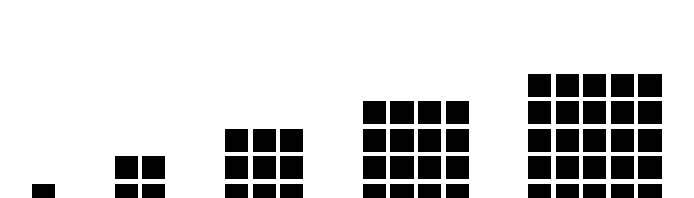
\begin{tikzpicture}[scale=0.35]
	\draw [ultra thick, white, fill=black] (0,0) rectangle (1,1);

	\begin{scope}[xshift=3cm]
	\foreach \x in {0,...,1}
	\foreach \y in {0,...,1}
	\draw [ultra thick, white, fill=black] (\x,\y) rectangle (\x+1,\y+1);
	\end{scope}

	\begin{scope}[xshift=7cm]
	\foreach \x in {0,...,2}
	\foreach \y in {0,...,2}
	\draw [ultra thick, white, fill=black] (\x,\y) rectangle (\x+1,\y+1);
	\end{scope}

	\begin{scope}[xshift=12cm]
	\foreach \x in {0,...,3}
	\foreach \y in {0,...,3}
	\draw [ultra thick, white, fill=black] (\x,\y) rectangle (\x+1,\y+1);
	\end{scope}

	\begin{scope}[xshift=18cm]
	\foreach \x in {0,...,4}
	\foreach \y in {0,...,4}
	\draw [ultra thick, white, fill=black] (\x,\y) rectangle (\x+1,\y+1);
	\end{scope}
\end{tikzpicture}
\caption{Perfect squares}
\label{fig:perfsq}
\end{figure}%

With other quadratic sequences, we can sometimes crack the code if we think about areas of rectangles. We'll look for pairs of integers that could give us the areas we're after, and then look for arithmetic sequences among those integers. The next thing you know, we'll have a non-recursive formula for the quadratic!

Let's go back to the other example we've been studying, the sequence $3, 8, 15, 24, 35, \dotsc$. This sequence came from the tile pattern at the start of \cref{sec:otherseq}. Go back and take another look at those pictures. What do you notice?

\begin{table}
\begin{tabular}{c|c|c}
Stage		& Number of Squares		& Dimensions of Rectangle	\\\hline
1			& 3							& $1 \times 3$		\\
2			& 8							& $2 \times 4$		\\
3			& 15						& $3 \times 5$		\\
4			& 24						& $4 \times 6$		\\
\end{tabular}
\end{table}%

In stage $n$, the size of the rectangle is $n$ units tall and $(n+2)$ units wide! So, we can use those two values to write an explicit formula:
\[a_n = n \cdot (n+2)\]
How cool is that?

\begin{boxex}
Write a non-recursive formula to generate the sequence $6, 12, 20, 30, 42, \dotsc$.

\exsoln\ It's not obvious how rectangles are related to these numbers, but if we assume we're looking for rectangles with integer side lengths, then there are a limited number of options.

For example, if the first number represents the area of a rectangle with integer side lengths, then it could be either a $1\times6$ rectangle or a $2\times3$ rectangle. Let's organize the different options in a table:

\begin{center}
\begin{tabular}{c|c|llll}
Stage		& Value		& \multicolumn{4}{l}{Possible Rectangles}
\\\hline
1			& 6			& $1 \times 6$
						& or\quad $2 \times 3$
						& ~
\\
2			& 12		& $1 \times 12$
						& or\quad $2 \times 6$
						& or\quad $3 \times 4$
\\
3			& 20		& $1 \times 20$
						& or\quad $2 \times 10$
						& or\quad $4 \times 5$
\\
4			& 30		& $1 \times 30$
						& or\quad $2 \times 15$
						& or\quad $3 \times 10$
						& or\quad $5 \times 6$
\\
5			& 42		& $1 \times 42$
						& or\quad $2 \times 21$
						& or\quad $3 \times 14$
						& or\quad $6 \times 7$
\\
\end{tabular}
\end{center}

Now comes the detective work. We are looking for patterns in the factors as they progress through the terms. We've highlighted the key patterns below.

\begin{center}
\begin{tabular}{c|c|llll}
Stage		& Value		& \multicolumn{4}{l}{Possible Rectangles}
\\\hline
1			& 6			& $1 \times 6$
						& or\quad $\colorbox{yellow!95!black}{2} \times \colorbox{green!95!black}{3}$
						& ~
\\
2			& 12		& $1 \times 12$
						& or\quad $2 \times 6$
						& or\quad $\colorbox{yellow!95!black}{3} \times \colorbox{green!95!black}{4}$
\\
3			& 20		& $1 \times 20$
						& or\quad $2 \times 10$
						& or\quad $\colorbox{yellow!95!black}{4} \times \colorbox{green!95!black}{5}$
\\
4			& 30		& $1 \times 30$
						& or\quad $2 \times 15$
						& or\quad $3 \times 10$
						& or\quad $\colorbox{yellow!95!black}{5} \times \colorbox{green!95!black}{6}$
\\
5			& 42		& $1 \times 42$
						& or\quad $2 \times 21$
						& or\quad $3 \times 14$
						& or\quad $\colorbox{yellow!95!black}{6} \times \colorbox{green!95!black}{7}$
\end{tabular}
\end{center}

Notice that the first set of factors (in yellow) form the arithmetic sequence $2, 3, 4, 5, \dotsc$, and the second set (in green) form the arithmetic sequence $3, 4, 5, 6, \dotsc$.

The yellow sequence is always one more than the term number. The green sequence is always two more than the term number. So, we have our explicit formula! \[a_n = (n+1)\cdot(n+2)\]
\end{boxex}

If these last two sections felt a bit overwhelming, don't worry. After we have some more algebraic tools in our toolbox, we'll return to quadratic relationships and describe them in more detail.


% % % % % % % % % % % % % % % % % % % % % % % % % % % % % % % % % % % % % % % % 
\chaptersummary

In this chapter we explored and extended the idea of a number pattern, with the result that we can now identify and describe certain kinds of patterns in detail. Already we have met the three key ``families'' of mathematical relationships that are at the heart of Algebra 1.

The linear family, represented in this chapter by the idea of an arithmetic sequence, will become our focus starting in \cref{ch:equations}. The exponential family, represented in this chapter by the geomertic sequences, will be our focus in \cref{ch:expofunc,,ch:expoexpr}. Quadratic sequences and the quadratic family will be in the spotlight starting in chapter \cref{ch:quadeq}.

Before we get into the individual families, though, we have a few more tools to add to our algebraic toolbox. Onward!
\chapter{Graphs and data}
\label{ch:graphs}

\chapquote{There is a magic in graphs. The profile of a curve reveals in a flash a whole situation -- the life history of an epidemic, a panic, or an era of prosperity. The curve informs the mind, awakens the imagination, convinces.}{Henry D. Hubbard\\US National Bureau of Standards}

In \cref{ch:sequences} we investigated pictures patterns (fractals by Koch and Sierpi\'nski, and patterns of made of square tiles) and used those pictures to generate sequences of numbers. We begin this chapter with a discussion of another way to represent our sequences of numbers visually: by making a coordinate graph. Then, we will extend these ideas to create visual representations of other mathematical objects, and of scientific (and other) data.

% % % % % % % % % % % % % % % % % % % % % % % % % % % % % % % % % % % % % % % % 
\section{Coordinate graphing}
\label{sec:coordgraph}

\Cref{fig:coordplane} summarizes the familiar landmarks of the \gls{coordinate plane}. We see the horizontal \gls{x-axis} and the vertical \gls{y-axis}. Using the two axes as number lines, we can locate \glspl{ordered pair} of numbers using the convention $(x,y)$. The points $(7, \umin2)$ and $(\umin6, 3)$ have been plotted as examples. The point $(0,0)$ where the the two axes meet, is a special point called the \gls{origin}.

\begin{figure}
	\centering
	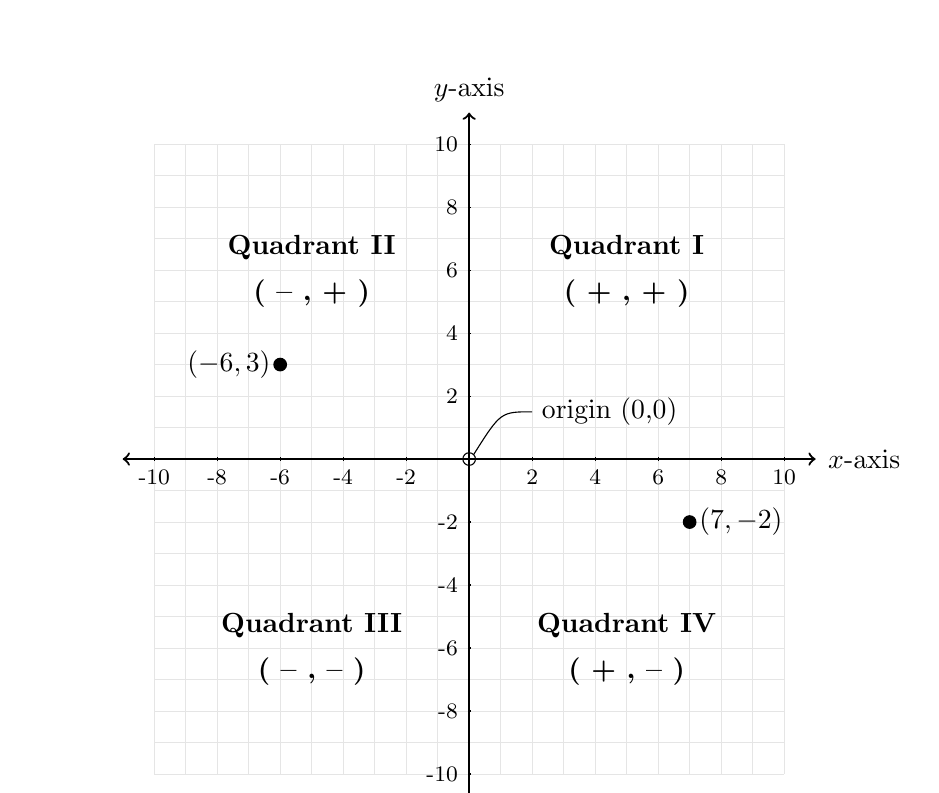
\begin{tikzpicture}[scale=0.4]
		%% grid setup
		\draw[very thin, color=gray!20] (-10,-10) grid (10, 10);
		\draw[<->,thick] (-11,0) -- (11,0);
		\draw (14,0) node[left]{$x$-axis};
		\draw (-14,0) node[right] {};
		\draw[<->,thick] (0,-11) -- (0,11) node[above]{$y$-axis};
		\foreach \x in {-10,-8,...,-2,2,4,...,10}
			\draw (\x,0.05) -- (\x,-0.05) node[below] {\footnotesize\x};
		\foreach \y in {-10,-8,...,-2,2,4,...,10}
			\draw (0.05,\y) -- (-0.05,\y) node[left] {\footnotesize\y};
		%% Quadrants
		\draw (5,6) node[above]{\bfseries Quadrant I}
			node[below]{\bfseries ( + , + 	)};
		\draw (-5,6) node[above]{\bfseries Quadrant II}
			node[below]{\bfseries ( -- , + )};
		\draw (-5,-6) node[above]{\bfseries Quadrant III}
			node[below]{\bfseries ( -- , -- )};
		\draw (5,-6) node[above]{\bfseries Quadrant IV}
			node[below]{\bfseries ( + , -- )};
		%% Origin
		\draw (0,0) circle (0.2);
		\draw (45:0.2) .. controls (1,1.5) .. (2,1.5) node[right]{origin (0,0)};
		%% Sample points
		\draw[fill] (7,-2) circle (0.2) node[right]{$(7, -2)$};
		\draw[fill] (-6,3) circle (0.2) node[left]{$(-6, 3)$};
	\end{tikzpicture}
	\caption{The coordinate plane and its important landmarks}
	\label{fig:coordplane}
\end{figure}

The axes chop the plane into four regions called \glspl{quadrant}, which are numbered starting in the upper right and moving counter-clockwise (as shown in the figure). The signs in parentheses indicate the signs of the $x$- and $y$-coordinates in each quadrant. The $x$-coordinates of the points in Quadrants I and IV are positive, while points in Quadrants II and III have $x$-coordinates that are negative. Points with positive $y$-coordinates lie in Quadrants I and II, while points with negative $y$-coordinates fall in Quadrants III and IV.\footnote{A point that lies on an axis doesn't actually lie in any of the four quadrants. So, the point $(4, 0)$ lives on the positive $x$-axis, but neither in Quadrant I nor in Quadrant IV.}

\begin{boxedexplore}[Pizza intersections]
Bob's friend Melvin ``Hambone'' Jones once worked delivering pizzas in his hometown of Euclid, Ohio. The town has streets running north-south and east-west.\footnote{Euclid, Ohio is also the home of the Polka Hall of Fame, though that has nothing to do with this problem. Also, Euclid isn't laid out in a grid as this problem implies, though it should be, given its name.}

Hambone is currently parked at the intersection we will call $(0,0)$. If he drives one block east, he will arrive at the intersection $(1,0)$. If he then turns right and drives one block south, he will arrive at the intersection $(1,-1)$.

Starting from $(0,0)$, describe are all the intersections that Hambone can reach by driving a total distance of exactly 10 blocks.
\end{boxedexplore}

\addtodoitem{Was there any Krumbli stuff in the sequences chapter? We need some continuity...}

\subsection{Graphing a sequence}

Our goal is to make a visual representation of a sequence on the coordinate plane.

``But,'' you may be asking yourself, ``a sequence is just a list of numbers. How do we make a coordinate graph, which needs coordinate pairs of numbers? It takes \textit{two numbers} to make a \textit{pair}!''

To graph a sequence, we use the term number as the $x$-coordinate and the term's value as the $y$-coordinate. Consider the sequence $1, 2, 4, 8, 16, 32,\dotsc$. The first term is 1, the second term is 2, and so on. We can organize this in a table, and write out the ordered pairs. Then, we can plot those ordered pairs and see a visual representation of our sequence!

\resizeplot{0}{0}{7}{40}

\bigskip
\begin{minipage}[c]{0.5\textwidth }
	\centering
	\begin{tabular}{|C{0.25\linewidth}|C{0.25\linewidth}|C{0.25\linewidth}|}
	\hline
	\text{Term No.} & \text{Term Value} & \text{Coord. Pair}\\
	x & y & (x,y)\\\hline
	1 & 1 & (1,1)\\
	2 & 2 & (2,2)\\
	3 & 4 & (3,4)\\
	4 & 8 & (4,8)\\
	5 & 16 & (5,16)\\
	6 & 32 & (6,32)\\\hline
	\end{tabular}
\end{minipage}%
%
\begin{minipage}[c]{0.5\textwidth }
	\centering
	\begin{tikzpicture}
		\begin{axis}[
			fullsize,
			defaultgrid,
			allminorticks,
			labeloutsideaxis,
			xlabel={Term No.},
			ylabel={Term Value},
		]
		\addplot[algpoints, blue] coordinates {(1,1)(2,2)(3,4)(4,8)(5,16)(6,32)};
		\end{axis}
	\end{tikzpicture}
\end{minipage}
\medskip

Recall that that sequence above, where the terms have a constant ratio, is called a geometric sequence. Let's look at an example of an arithmetic sequence, in which the terms have a constant difference. For example, consider the sequence $8, 13, 18, 23, 28, 33,\dotsc$. This sequence produces the following table and graph:

\bigskip
\begin{minipage}[c]{0.5\textwidth }
	\centering
	\begin{tabular}{|C{0.25\linewidth}|C{0.25\linewidth}|C{0.25\linewidth}|}
	\hline
	\text{Term No.} & \text{Term Value} & \text{Coord. Pair}\\
	x & y & (x,y)\\\hline
	1 & 8 & (1,8)\\
	2 & 13 & (2,13)\\
	3 & 18 & (3,18)\\
	4 & 23 & (4,23)\\
	5 & 28 & (5,28)\\
	6 & 33 & (6,33)\\\hline
	\end{tabular}
\end{minipage}%
%
\begin{minipage}[c]{0.5\textwidth }
	\centering
	\begin{tikzpicture}
		\begin{axis}[
			fullsize,
			defaultgrid,
			allminorticks,
			labeloutsideaxis,
			xlabel={Term No.},
			ylabel={Term Value},
		]
		\addplot[algpoints, red] coordinates {(1,8)(2,13)(3,18)(4,23)(5,28)(6,33)};
		\end{axis}
	\end{tikzpicture}
\end{minipage}
\medskip

Finally, let's see what a quadratic pattern looks like. For example, the perfect squares form a quadratic sequence $1, 4, 9, 16, 25, 36, \dotsc$. Their table and graph go like this:

\bigskip
\begin{minipage}[c]{0.5\textwidth }
	\centering
	\begin{tabular}{|C{0.25\linewidth}|C{0.25\linewidth}|C{0.25\linewidth}|}
	\hline
	\text{Term No.} & \text{Term Value} & \text{Coord. Pair}\\
	x & y & (x,y)\\\hline
	1 & 1 & (1,1)\\
	2 & 4 & (2,4)\\
	3 & 9 & (3,9)\\
	4 & 16 & (4,16)\\
	5 & 25 & (5,25)\\
	6 & 36 & (6,36)\\\hline
	\end{tabular}
\end{minipage}
%
\begin{minipage}[c]{0.5\textwidth }
	\centering
	\begin{tikzpicture}
		\begin{axis}[
			fullsize,
			defaultgrid,
			allminorticks,
			labeloutsideaxis,
			xlabel={Term No.},
			ylabel={Term Value},
		]
		\addplot[algpoints, violet] coordinates {(1,1)(2,4)(3,9)(4,16)(5,25)(6,36)};
		\end{axis}
	\end{tikzpicture}
\end{minipage}
\medskip

Take a moment to compare the graphs of these three sequences. How are they alike? How are they different?

\subsection{Features of the graph of a sequence}

Note that since the term number is always greater than 0, our graphs only show the positive part of the $x$-axis. We'll soon see that this is an artificial limitation that doesn't apply to most situations: the negative part of the $x$-axis is just as important as the positive part.

Note also that we haven't connected the dots. A sequence has a first term and a second term, but no one-and-a-halfth term. So, we shouldn't have any points with $x$-coordinates in between the natural numbers. We'll soon see that this is an artificial limitation, too. Fractional $x$-values are appropriate for most rules.

If we change our point of view and allow the input to be any real number, we will have turned our sequence into a mathematical relationship called a \gls{function}.\footnote{Actually, a sequence is \textit{already} a function. The distinction we make here has to do with what kinds of input values are allowed. Later, once we have some additional concepts under our belts, we'll talk about a sequence as ``a function whose domain is the natural numbers''.} We'll discuss the details of what functions are (and what they are not) in \cref{ch:functions}.


% % % % % % % % % % % % % % % % % % % % % % % % % % % % % % % % % % % % % % % % 
\section{Algebraic expressions}
\label{sec:algexpr}

\begin{boxedexplore}[Don't take all year]
Find three natural numbers $x$, $y$, and $z$ which satisfy the equation $28x + 30y + 31z = 365$. Can you find more than one set of numbers $x,y,z$ that satisfy the equation?
\end{boxedexplore}

In \cref{ch:numbers} we used the order of operations to simplify numeric expressions, which are made up of numbers and arithmetic operators. For example, \[3\cdot4-8(4^2-1)\] is a numeric expression. It contains only numbers and operators and, in the end, it simplifies down to a single number.\footnote{Spoiler alert: It's $-108$.} An \gls{algebraic expression} on the other hand can contain letters in addition to numbers and operators, for example \[3x - 5y + 18.\] These letters, called \glspl{variable}, stand in for numbers that we don't know or which may change.

\begin{boxeddef}[Variable]
A representation of a value that can change. In algebra, variables are often represented by letters. We usually use letters from the Latin alphabet ($a, b, c, d,\dotsc$), but sometimes also use other symbols, such as letters from the Greek alphabet ($\alpha, \beta, \gamma, \delta, \dotsc$).
\end{boxeddef}

\begin{boxeddef}[Algebraic expression]
A symbolic representation of mathematical operations that can involve both numbers and variables.
\end{boxeddef}

\subsection{Numbers and variables}

In your mathematical career so far, you have probably worked with letters that stand in for numbers. Recall the formula for the circumference of a circle: \[C = \pi d.\]
This formula explains the relationship between $d$, which stands in for the diameter of some circle, and $C$, which stands for the circumference of that circle. The letters $d$ and $C$ are variables. They stand in for numbers that can change, depending on which circle we're talking about.\footnote{Note that $\pi$ is \textit{not} a variable. We use a (Greek) letter in this case not because the value of $\pi$ might change, but because it's an irrational number that is impossible to write out in full. We often use letters to stand in for mathematical objects that are inconvenient, sometimes impossible, to write down in another way: $e$, $i$, $\phi$, and $\aleph_0$ each has special mathematical meaning.}

Once we start to introduce letters into our expressions, we have to discuss some standard notation and terminology. As we have seen, we don't usually write any multiplication symbol when multiplying a number by a variable. Rather than writing $3\cdot x$ or $3(x)$, we can write $3x$ without anything in between.

An algebraic expression that is built using only multiplication (or division) is called a \gls{term}. For example, $3x$ and $\frac{1}{2}m$ are terms. On the other hand, the expression $3x+2y$ is not a term because it includes addition. In fact, this expression is the sum of two terms.

\begin{boxeddef}[Term]
An algebraic expression that represents only multiplication and division between variables and constants (numbers).
\end{boxeddef}

When we have the product of a number and a variable, like $3x$ or $\umin11g$, the number part is called the \gls{coefficient} of the term. So, the coefficient of $3x$ is 3, and $\umin11$ is the coefficient of $\umin11x$. If we have a variable all alone without a number attached, like $y$ or $w$, then we picture a ``phantom 1'' lurking there as the coefficient: $y$ is the same as $1y$, and $1w$ is the same as $w$.

\begin{boxeddef}[Coefficient]
The numerical factor in a term with a variable. If no number is explicitly written, the coefficient is understood to be 1.
\end{boxeddef}

\subsection{Evaluating algebraic expressions}

A variable is a ``placeholder'' that stands in for a number. We can only determine the value of an algebraic expression if we know what numbers the different variables represent.

Consider the expression $3x$. If we know that $x$ represents $15$, then we can \gls{evaluate} the expression $3x$ in the case that $x = 15$. In that case, it must be that $3x = 3(15) = 45$.

When we evaluate an algebraic expression, we substitute in values for its variables, and then simplify the resulting numeric expression using the order of operations. It is a really good habit always to use parentheses when substituting numeric values for variables. This can avoid confusion about negative numbers!

\begin{boxedex}
\label{ex:evaluating}
Evaluate the expressions (a) $6x+ 4$, and (b) $x^2 - 5$ for the $x$ values 3, $\umin1$, and $\frac{1}{2}$.

\exsoln{}
\begin{enumerate}[label={(\alph*)}]
\item To evaluate the expression $6x + 4$ for the given values of $x$, we simply substitute and follow the order of operations.
\[
\begin{array}{lllll}
\text{When $x=3$:}
&
&
\text{When $x=\umin1$:}
&
&
\text{When $x=\frac{1}{2}$:}
\\ % content
\begin{aligned}
6x + 4 & = 6(3) + 4\\
& = 18 + 4\\
& = 22
\end{aligned}
&
\qquad\qquad
&
\begin{aligned}
6x + 4 & = 6(\umin1) + 4\\
& = \umin6 + 4\\
& = \umin2
\end{aligned}
&
\qquad\qquad
&
\begin{aligned}
6x + 4 & = 6\left(\tfrac{1}{2}\right) + 4\\
& = 3 + 4\\
& = 7
\end{aligned}
\end{array}
\]

\item We do the same in order to evaluate $x^2 - 5$ for the given $x$ values.
\[
\begin{array}{lllll}
\text{When $x=3$:}
&
&
\text{When $x=\umin1$:}
&
&
\text{When $x=\frac{1}{2}$:}
\\ % content
\begin{aligned}
x^2 - 5 & = (3)^2 - 5\\
& = 9 - 5\\
& = 4
\end{aligned}
&
\qquad\qquad
&
\begin{aligned}
x^2 - 5 & = (\umin1)^2 - 5\\
& = 1 - 5\\
& = \umin4
\end{aligned}
&
\qquad\qquad
&
\begin{aligned}
x^2 - 5 & = \left(\tfrac{1}{2}\right)^2 - 5\\
& = \tfrac{1}{4} - 5\\
& = -\tfrac{19}{4}
\end{aligned}
\end{array}
\]
\end{enumerate}
\end{boxedex}

Note how the parentheses help out when $x = \umin1$! Without those parentheses, we would have run the risk of making the most common mistake in Algebra 1: remember the difference between $(\umin1)^2$ and $\umin1^2$.

%%Speaking of parentheses: Remember that a graphing calculator will follow the order of operations. That means that we need to use the proper notation for our intentions. If our intent is to raise $\umin2$ to the fourth power, we had better not write $\umin2^4$ but rather write $(\umin2)^4$ with parentheses!

%%% WHAT TO DO WITH THIS STUFF?
%(2) NO WORK NO CREDIT always applies. If you are wondering how to show work when you have a calculator at your disposal, here is what I want. Be sure to write down what you are having the calculator do for you. Say you need to add 3/4 to 1/2 and then divide it by 7. You need to write down ( 3/4 + 1/2) / 7. That way I know what you are doing to solve the problem.
%
%(3) SIMPLIFY COMPLETELY always applies. Your answers need to be simplified improper fractions, unless the solution is in a context or I ask you specifically for a different format. Be sure to read questions carefully.
%
%(4) A few things we will go over in class over about operating the TI-84+:
%a. what button to use to designate a negative
%b. what to do when you have a syntax error
%c. how to enter fractions and other short-cut keys
%d. how to raise to powers other than 2 e. how to clear ram
%f. how to correct the mode/setting
%g. how to recall, delete, and insert
%h. how to simplify answers
%
%We will go over more things your calculator can do for you as they become necessary in class.

% MOVE TO FUNCTIONS CHAPTER...?
%Using the formula for the formula for arithmetic, I wrote the rule an = 12 + 3 (n – 1), which I convert to the equation y = 12 + 3 (x – 1). Now let's graph it in a standard window. You should be able to see why they call this relationship linear. Arithmetic sequences always graph to be lines, not vertical or horizontal though. Arithmetic sequences always increase or decrease by the exact same value, which means they have a constant rate of change.

% % % % % % % % % % % % % % % % % % % % % % % % % % % % % % % % % % % % % % % % 
\section{Graphing a function}
\label{sec:graphingfunc}

The graphs of sequences that we created earlier were quite limited. Since sequences use only the natural numbers as input values, the only points we had available to plot were the points where $x = 1, 2, 3, 4, \dotsc$. But now, knowing how to evaluate algebraic expressions, we can create more complete graphs by choosing a wider variety of $x$-values.

\begin{boxedexplore}[Extending our sequences]
Write a zero-based explicit rule for the arithmetic sequence shown below (this is the second example from \cref{sec:coordgraph}). First write the rule in terms of $n$ and $a_n$, then translate your rules into a graphable format in terms of $x$ and $y$.
\[8, 13, 18, 23, 28, \dotsc\]
The given sequence represents the $y$-values of the rule for the $x$-values 1, 2, 3, 4, and 5. Evaluate your rule for the $x$-values 0, -1, -2, -3, -4, and -5. Then, plot these 11 points on a coordinate grid.
\end{boxedexplore}

The rule for the sequence in the startup exploration is $a_n = 5n + 3$, or in terms of $x$ and $y$, we have the rule $y = 5x + 3$. To create the coordinate graph, we can substitute the different $x$-values into the rule and compute the $y$-values. The middle column in the table below is our ``process column'' in which we substitute an $x$-value and compute the corresponding $y$-value. 

\begin{table}
\begin{tabular}{|C{2cm}|C{6cm}|C{2cm}|}
	\hline
	x & y = 5 x + 3& (x,y)\\\hline
	0 		& y = 5(0) + 3 = 0 + 3 = 3 & (0,3)\\
	\umin1 & y = 5(\umin1) + 3 = \umin5 + 3 = \umin2  & (\umin1,\umin2)\\
	\umin2 & y = 5(\umin2) + 3 = \umin10 + 3 = \umin7  & (\umin2,\umin7)\\
	\umin3 & y = 5(\umin3) + 3 = \umin15 + 3 = \umin12  & (\umin3,\umin12)\\
	\umin4 & y = 5(\umin4) + 3 = \umin20 + 3 = \umin17  & (\umin4,\umin17)\\
	\umin5 & y = 5(\umin5) + 3 = \umin25 + 3 = \umin22  & (\umin5,\umin22)\\\hline
\end{tabular}
\end{table}

In the end, we generate 6 new coordinate pairs, which we can graph alongside the five points that we were given.

\resizeplot{-5}{-25}{5}{29}
\begin{center}
\begin{tikzpicture}
	\begin{axis}[
		medsize,
		defaultgrid
	]
	\addplot[algpoints, red] coordinates {(-5,-22)(-4,-17)(-3,-12)(-2,-7)(-1,-2)(0,3)(1,8)(2,13)(3,18)(4,23)(5,28)};
	\end{axis}
\end{tikzpicture}
\end{center}

Can you anticipate the location of the point that we plot when $x = \frac{1}{3}$? What about when $x = \umin\frac{5}{2}$? What would our graph look like if we used all of the points in $\R$ as the $x$-values?

When we use all of the real numbers as input to the rule $y = 5x + 3$, the resulting graph is a straight line. Of course, it would be impossible to actually plot \textit{all} of the points (there are infinitely many of them), but the pattern holds true, and so we can replace the dots with a continuous line.

\begin{center}
\begin{tikzpicture}
	\begin{axis}[
		medsize,
		defaultgrid
	]
	\addplot[algcurve, red, domain=-5:5] (\x,5*\x+3);
	\end{axis}
\end{tikzpicture}
\end{center}

The rules below correspond to the other two sequences we studied in \cref{sec:coordgraph}. Under each rule is the graph that is created when we plot the rule over $\R$.

\begin{figure}
\begin{minipage}[c]{0.49\textwidth }
	\centering
	$y = 2^x$\par\medskip
	\begin{tikzpicture}
		\begin{axis}[
			fullsize,
			defaultgrid
		]
		\addplot[algcurve, blue, domain=-5:4.75] (\x,2^\x);
		\end{axis}
	\end{tikzpicture}
\end{minipage}
%
\begin{minipage}[c]{0.49\textwidth }
	\centering
	$y = x^2$\par\medskip
	\begin{tikzpicture}
		\begin{axis}[
			fullsize,
			defaultgrid
		]
		\addplot[algcurve, violet, domain=-5:5] (\x,\x^2);
		\end{axis}
	\end{tikzpicture}
\end{minipage}
\end{figure}

Are you surprised by these two graphs? Back in \cref{sec:coordgraph}, the graphs of these two sequence looked similar. But, we were only looking at the first quadrant! Their graphs are very different for negative values of $x$.

The moral of the story is that when we are asked to graph an equation by hand, we need to use a variety of different $x$-values, including negative numbers and fractions. Often, a problem will clearly indicate exactly what values to use.

\subsection{Criteria for high quality graphs}

In algebra we make a distinction between ``sketching'' and ``graphing''. A sketch is just a quick drawing and it doesn't need to be super accurate. A sketch can drawn on notebook paper (or scribbled on a napkin).

On the other hand, a proper graph is meant to communicate something to the viewer. A graph must be accurately drawn on graph paper. The most important features of whatever we're graphing -- a sequence, a function, a plot of a data set -- must be clear, accurate, and neatly represented. Here are some guidelines for creating high-quality graphs.

High quality graphs should be drawn on graph paper. An individual graph does not have to take up an entire piece of graph paper, although it should be drawn large enough to be easily understood.

Use a ruler or straightedge to make straight lines, in particular the coordinate axes or any linear data. Plus, we should draw arrowheads on anything that continues forever. This includes axes, lines, and curves (note the arrowheads in the graphs above).

Be mindful when choosing a scale for the axes. Choose a scale that fits the data and ensures that your graph shows all important features of the curve. The origin does not necessarily need to be in the center of the grid. For example, if we are plotting data that includes only positive values, then we only need the first quadrant. The origin in this case might be in the lower left-hand corner of the graph.

Scales for the $x$- and $y$-axes can be different, and in some cases must be different, so this can take a little bit of planning. The scale must be the same for the whole length of an axis, and cannot have any ``jumps'' or ``breaks''. Changes in the scale will distort the shape of the graph, which defeats the purpose! Compare the two grids below. The grid on the left is fine, but the grid on the right includes a common mistake. Can you identify the problem?

\begin{minipage}{0.5\linewidth}
	\centering
	OK!\par
	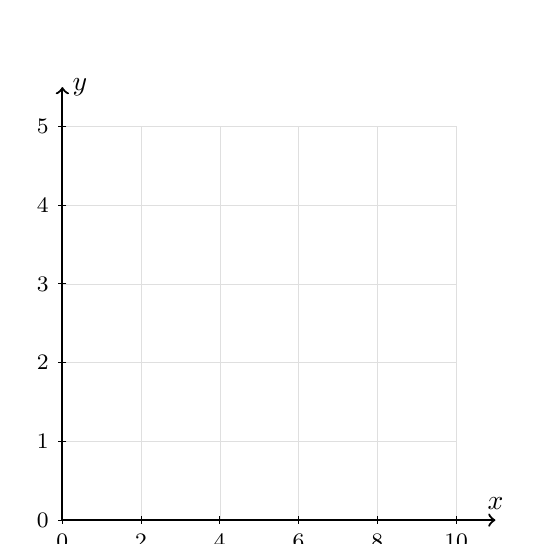
\begin{tikzpicture}[scale=1]
		%% grid setup
		\draw[very thin, color=gray!25] (0,0) grid (5,5);
		\draw[->,thick] (0,0) -- (5.5,0) node[above]{$x$};
		\draw[->,thick] (0,0) -- (0,5.5) node[right]{$y$};
		\foreach \x in {0,2,...,10}
			\draw (\x/2,0.05) -- (\x/2,-0.05) node[below] {\footnotesize\x};
		\foreach \y in {0,1,...,5}
			\draw (0.05,\y) -- (-0.05,\y) node[left] {\footnotesize\y};
	\end{tikzpicture}
\end{minipage}
%
\begin{minipage}{0.5\linewidth}
	\centering
	Not OK!\par
	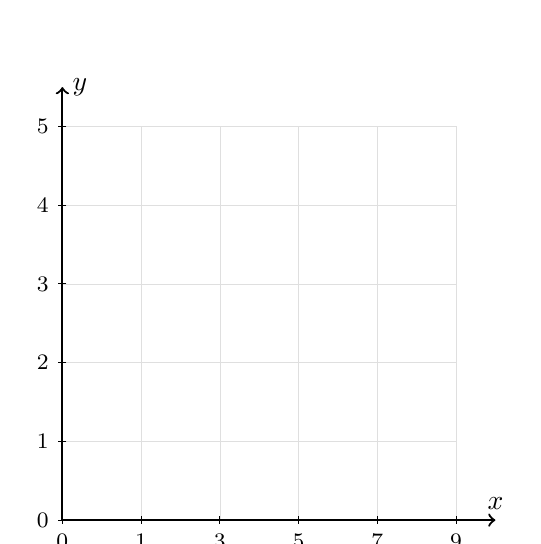
\begin{tikzpicture}[scale=1]
		%% grid setup
		\draw[very thin, color=gray!25] (0,0) grid (5,5);
		\draw[->,thick] (0,0) -- (5.5,0) node[above]{$x$};
		\draw[->,thick] (0,0) -- (0,5.5) node[right]{$y$};
		\foreach \x in {0,1}
			\draw (\x,0.05) -- (\x,-0.05) node[below] {\footnotesize\x};
		\draw (2,0.05) -- (2,-0.05) node[below] {\footnotesize3};
		\draw (3,0.05) -- (3,-0.05) node[below] {\footnotesize5};
		\draw (4,0.05) -- (4,-0.05) node[below] {\footnotesize7};
		\draw (5,0.05) -- (5,-0.05) node[below] {\footnotesize9};
		\foreach \y in {0,1,...,5}
			\draw (0.05,\y) -- (-0.05,\y) node[left] {\footnotesize\y};
	\end{tikzpicture}
\end{minipage}
\medskip

High quality graphs are clearly labeled. The scale should be indicated on the axes, and the axes should be labeled. For graphs of equations, this might mean simply labeling the axes $x$ and $y$. When plotting data, include more informative names like ``time'' or ``distance''.

A final question to consider regarding data points: to connect or not to connect? In the next section, we will discuss this question in some detail. But we've already seen some important pieces of this puzzle. When we have a sequence, or other data that skips values, we should not connect the points.

If we do want to connect the points, say, when graphing a funcction by plotting some sample points, we should connect with a smooth curve and \textit{not} individual line segments. If we use a straight line to connect points, then we are telling our audience that the data in between the points is linear, which may not be the case! Go back and have a look at the graph of $y=x^2$. It doesn't come to a point at the bottom. Rather it's a smooth curve that passes through the origin.

%\begin{boxedexplore}[Extended exploration: Big graphs]
%\addtodoitem{Click here to visit the extended exploration: Big Graphs}
%\end{boxedexplore}
\addtodoitem{Link to extended exploration: Big graphs}

% % % % % % % % % % % % % % % % % % % % % % % % % % % % % % % % % % % % % % % % 
\section{Patterns in data}
\label{sec:patternsindata}

The graphs that we have been working with so far have been very orderly. Technical and scientific data, however, are not always so tidy. Data can be noisy, messy, and incomplete. We will need some tools that can help us to see and describe patterns that may (or may not) exist in experimental data.

%\begin{boxedexplore}[Extended exploration: Who is the best age guesser?]
%\addtodoitem{Click here to visit the extended exploration: Who Is the Best Age Guesser?}
%\end{boxedexplore}
\addtodoitem{Link to extended exploration: Age guesser}

\begin{boxedexplore}[Water consumption]
The graph shown in \cref{fig:waterconsumption} depicts water consumption in Edmonton, capital of the Canadian province of Alberta, during the gold medal men's ice hockey game at the 2010 Winter Olympics in Vancouver. The game was played between Canada and United States.

Water consumption during the game is shown in blue, while data from the same time period on the previous day is shown in green.

Write down anything you notice or wonder about the data presented in this graph.

A few notes: Ice hockey games are played in three 20-minute periods with breaks in between. In this particular game, the score was tied at the end of regular play. Canada scored the winning goal in overtime and was then awarded the gold medal.
\end{boxedexplore}

\begin{figure}[htbp]
\centering\bigskip
\begin{tikzpicture}
\begin{axis}[
		width=0.75\textwidth,
		ylabel={\footnotesize Customer Water Demand (megaliters)},
		ymin=300,
		ymax=500,
		ytick={320,340,...,480},
		ytick pos=left,
		ymajorgrids,
		xmin=0,
		xmax=6,
		xtick={0,...,6},
%		xtick pos=left,
		xticklabels={12:00, 13:00, 14:00, 15:00, 16:00, 17:00, 18:00},
		tick label style={
			font=\footnotesize
		},
		legend style={
			font=\footnotesize,
			legend pos=north west,
			draw=black!25
		},
		enlargelimits=false
	]
	\addplot[thick, green!80!black] table [x=time, y=day1, col sep=comma] {data/water.csv};
	\addlegendentry{27 Feb 2010};
	\addplot[thick, blue] table [x=time, y=day2, col sep=comma] {data/water.csv};
	\addlegendentry{28 Feb 2010};
\end{axis}
\end{tikzpicture}
\caption{Water consumption in Edmonton on 27 and 28 February 2010 (source: \href{http://www.epcor.com}{EPCOR})}
\label{fig:waterconsumption}
\end{figure}

%\begin{figure}[!htbp]
%	\centering
%	{\color{black!25}\fbox{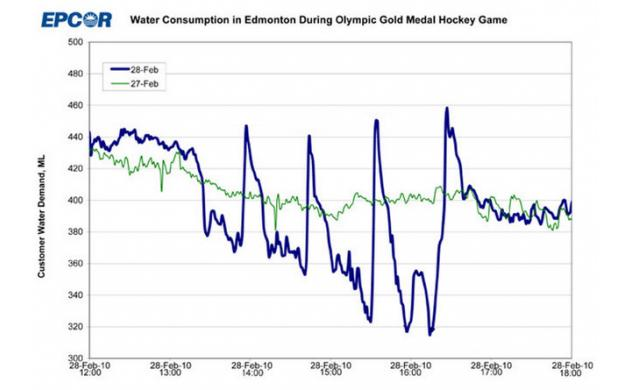
\includegraphics[scale=0.65]{canadianwater.png}}}
%	\caption{Water consumption in Edmonton during the 2010 Olympic men's ice hockey final}
%	\label{fig:waterhockey}
%\end{figure}

%\begin{boxedexplore}[Guess Your Weight]
%\begin{minipage}[t]{0.7\textwidth}
%\vspace{0pt}
%Alphonse the Amazing has a Guess-Your-Weight booth on the carnival midway at the Cheeseville Zoo. To play, people pay \$1, Alphonse guesses their weight, and then they step on a scale (only the most self-confident people play this game). If Alphonse's guess is off by more than 5 pounds (over or under), they win a prize.
%
%The table shows the guessed weight and actual weight of 15 brave souls who played the game.
%
%Evaluate Alphonse's skill as a weight guesser, based on the evidence presented in the table. What feedback would you give him?
%\end{minipage}%
%%
%\begin{minipage}[t]{0.3\textwidth}
%\vspace{0pt}
%\raggedleft
%\begin{tabular}{|C{1.55cm}|C{1.55cm}|}
%\hline
%\text{\footnotesize Guessed Wt} & \text{\footnotesize Actual Wt}
%\\\hline
%75 & 71\\
%90 & 88\\
%100 & 99\\
%130 & 121\\
%140 & 126\\
%175 & 159\\
%95 & 93\\
%115 & 112\\
%125 & 118\\
%150 & 134\\
%80 & 78\\
%160 & 145\\
%180 & 163\\
%85 & 82\\
%170 & 153\\\hline
%\end{tabular}\par
%\end{minipage}
%\end{boxedexplore}

In the graph of Edmonton water consumption, the amount of water being used varies depending on the time of day (not the other way around). We say that ``time of day'' is the \textit{independent variable} and ``water demand'' is the \textit{dependent variable}. 

\begin{boxeddef}[Independent variable]
A variable whose values affect the values of another variable. In a graph of the relationship between two variables, the quantity represented on the horizontal axis (the $x$-axis) usually represents the independent variable.
\end{boxeddef}

\begin{boxeddef}[Dependent variable]
A variable whose values depend on the values of another variable. In a graph of the relationship between two variables, the quantity represented on the vertical axis (the $y$-axis) usually represents the dependent variable.
\end{boxeddef}

\subsection{Correlation}

We can compare just about any two quantities. One way to do this is with a graph called a \gls{scatter plot}.

\begin{boxeddef}[Scatter plot]
A graph that relates data of two different sets. The two sets of data are displayed as ordered pairs.
\end{boxeddef}

Suppose we wish to compare, say, the height and weight for all of the players on the top two 2010 Olympic men's ice hockey teams. Let's make a graph comparing every player's height and weight as ordered pairs: (height, weight). This graph is shown on the left in \cref{fig:hockeystats}.\footnote{Data from the International Olympic Committee, as reported in \href{http://en.wikipedia.org/wiki/Ice_hockey_at_the_2010_Winter_Olympics}{Wikipedia}.}

While we're at it, let's make another comparison. The graph on the right in \cref{fig:hockeystats} plots every player's height and jersey number as ordered pairs (height, jersey number). What do you notice about these two graphs? How are they the same? How are they different?

\begin{figure}
\label{fig:hockeystats}
\caption{Comparing the Canadian and US men's ice hockey teams (2010 Winter Olympics).}
%
\begin{minipage}{0.45\linewidth}
% (height, weight)
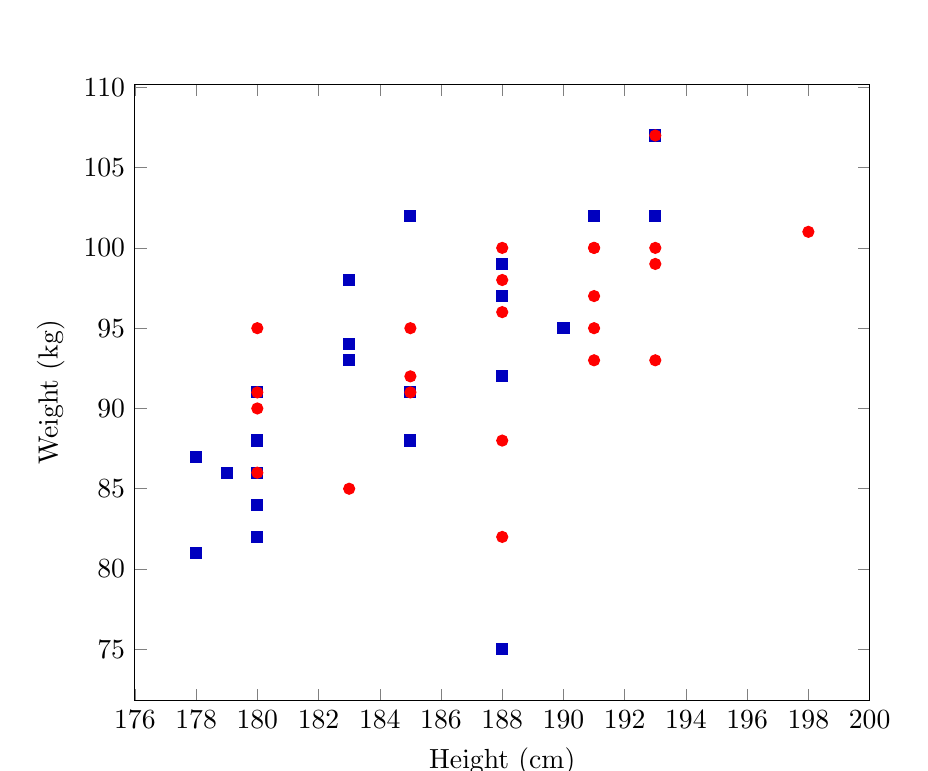
\begin{tikzpicture}[domain=150:200]
	\begin{axis}[
		legend style={
			font=\footnotesize,%
			legend pos=south east,%
			legend cell align=left,%
			/tikz/every even column/.append style={column sep=1em},%
			draw=black!25,%
		},%
		legend columns=-1,
		legend to name=namedhockeylegend,
		width=0.9\linewidth,%
		xlabel={Height (cm)},%
		ylabel={Weight (kg)}%
	]
	\addplot[%
		scatter/classes={
			1={mark=square*, blue!75!black},%
			2={mark=*, red}
		},
		scatter,
		only marks,
		scatter src=explicit symbolic]
      table[x=x, y=y, meta=label] {
	x		y		label
	188		75		1
	185		91		1
	180		91		1
	183		98		1
	193		107		1
	185		102		1
	188		99		1
	178		87		1
	185		88		1
	190		95		1
	191		102		1
	183		94		1
	180		84		1
	179		86		1
	178		81		1
	188		92		1
	180		82		1
	185		91		1
	193		102		1
	180		86		1
	180		88		1
	188		97		1
	183		93		1
	188		98		2
	188		82		2
	191		93		2
	180		86		2
	185		92		2
	183		85		2
	185		91		2
	198		101		2
	191		100		2
	191		97		2
	188		88		2
	180		90		2
	193		100		2
	191		100		2
	185		95		2
	188		100		2
	180		95		2
	193		99		2
	180		91		2
	191		95		2
	193		93		2
	193		107		2
	188		96		2
	};
	\legend{Team USA, Team Canada};
	\end{axis}
\end{tikzpicture}
\end{minipage}
%
\begin{minipage}{0.45\linewidth}
% (height, jersey number)
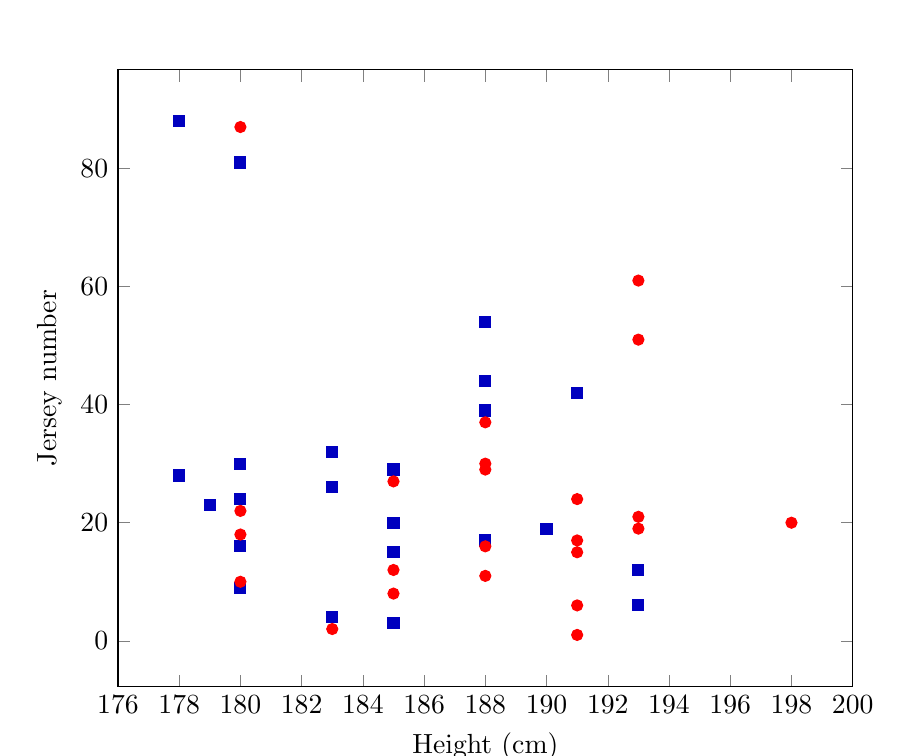
\begin{tikzpicture}[domain=150:200]
	\begin{axis}[
		width=0.9\linewidth,%
		xlabel={Height (cm)},%
		ylabel={Jersey number}%
	]
	\addplot[%
		scatter/classes={
			1={mark=square*, blue!75!black},%
			2={mark=*, red}
		},
		scatter,
		only marks,
		scatter src=explicit symbolic]
      table[x=x, y=y, meta=label] {
	x		y		label
	188		39		1
	185		29		1
	180		30		1
	183		4		1
	193		6		1
	185		3		1
	188		44		1
	178		28		1
	185		20		1
	190		19		1
	191		42		1
	183		32		1
	180		24		1
	179		23		1
	178		88		1
	188		17		1
	180		81		1
	185		15		1
	193		12		1
	180		9		1
	180		16		1
	188		54		1
	183		26		1	
	188		30		2
	188		29		2
	191		1		2
	180		22		2
	185		8		2
	183		2		2
	185		27		2
	198		20		2
	191		17		2
	191		6		2
	188		37		2
	180		87		2
	193		51		2
	191		15		2
	185		12		2
	188		11		2
	180		10		2
	193		61		2
	180		18		2
	191		24		2
	193		21		2
	193		19		2
	188		16		2
	};
	%\legend{Team USA, Team Canada};
	\end{axis}
\end{tikzpicture}
\end{minipage}
\ref{namedhockeylegend}
\end{figure}

Notice that the graph of weight and height has a clear upward slant. This seems reasonable: the taller someone is, the more we might expect that person to weigh. There are some data points that don't fit the trend, but generally speaking the data points are increasing as we look toward the right on the graph. We say that this data shows a positive \gls{correlation}.

\begin{boxeddef}[Correlation]
A trend between two sets of data, as seen in a scatter plot. A trend can show positive, negative, or no correlation. Positive correlation shows an \gls{increasing} trend in data. Negative correlation shows a \gls{decreasing} trend in data.
\end{boxeddef}

The graph of jersey number versus height is more of a blob. There's no clear trend in this data, and so we say that is shows \textit{no correlation}. This makes sense, too: there's no logical connection between a player's height and the number they wear on their shirt.

A third possibility would be data which shows a negative correlation, meaning that the data are decreasing as we look towards the right on the graph. Can you imagine two variables that might show a negative correlation when compared on a scatter plot?

Graphing experimental data on a scatter plot helps us to see if there is a relationship between variables. If there is, a pattern will emerge in the graph. The points will fall (approximately) in a line or a curve and will have a correlation. A key thing to remember when it comes to looking at data is that ``correlation does not imply causation''. In other words: If we see that two variables are correlated, we might be tempted to assume that the change in one variable \textit{causes} the change in the other. This is sometimes true, but not always.

%If the scatter plot shows a positive correction, it means that as the independent variable increases, the dependent variable increases. If the scatter plot shows a negative correlation, it means that as the independent variable increases, the dependent variable decreases. If a scatter plot shows no correlation, it indicates that there is no relationship between the two variables.

For example, it seems reasonable to believe that a change in height will cause a change in weight. But, there is data that shows a positive correlation between ``consumption of mozzarella cheese per person'' and ``number of civil engineering doctorates awarded''. This has to be a coincidence! There's no (good) reason to think that changing one of these variables would cause a change in the other one.\footnote{This fact is courtesy of the website \href{http://www.tylervigen.com/view_correlation?id=3890}{Spurious Correlations}, which has many graphs of interesting and ridiculous data that show correlation but not causation. Sometimes, it's fun to try to ``explain'' the correlation. Perhaps in this case the increase in mozzarella cheese consumption is due to an increase in takeout pizza demand, which leads to more pizza delivery shops, which in turn requires more roads, which means we need more engineers to design them.}

\subsection{Continuous and discrete data}

When we drew the graph of a sequence, we didn't connect the dots. A sequence has a first term and a second term, but no one-and-a-halfth term. The $x$-values have no ``in-betweens''.

Similarly, imagine a graph showing ``time'' as the independent variable and ``number of hockey players on the ice'' as the dependent variable. In this case, the $y$-values would have no ''in-betweens''. There could be 11 players or 12 players on the ice, but never 11.5 players. This is called \gls{discrete data}.

\begin{boxeddef}[Discrete data]
Data for which it doesn't make sense for measurements to exist between given data points. Discrete data often involves \textit{counting items}, such at the number of cars in a parking lot over time. 
\end{boxeddef}

On the other hand, when we started to picture the graph of a rule that could accept any real number as input, we drew a continuous line on the graph. The graph of water consumption in Edmonton, is jagged, spiky, and irregular -- but it's a continuous line. We can measure how much water has been used at any point in time, and we can measure the amount of water in fractions of a unit. We call this \gls{continuous data}.

\begin{boxeddef}[Continuous data]
Data that has no holes, gaps, or breaks. Continuous data often involves \textit{measuring some value} where measurements exist (and may change) between data points. For example, a person's height over time.
\end{boxeddef}

%The graphs we saw in the last section (straight lines and smooth curves) are quite easy to describe mathematically. For instance, we know how to write rules for sequences, and sequences were what led us to graph those curves in the first place. It's hard -- and sometimes impossible -- to write a neat rule for this data. So, we have developed some other terminology to describe sometimes-messy data.

%The key to knowing the difference between continuous and discrete data is to ask whether the data involves measuring or counting.
Consider a data collection scenario in which we want to graph ``Bob's distance from home at any given time (in kilometers)''. Bob is always a certain distance away from home (perhaps 0 km, if he is at home), and he could be any distance (even fractions of a kilometer). So, this is continuous data and our graph should be an unbroken line.

Now consider the scenario in which we graph ``number of customers in line at the cheese counter at Middle Market.'' Although there is always a certain number of people in line (maybe zero), there can never be 5.7 people in line. We must count people, and so this data is discrete. Our graph would have to ``jump'' from 5 people to 6 people without going through the in-between values.

\resizeplot{0}{0}{7}{7}
\begin{figure}
\label{fig:continuousvsdiscrete}
\caption{Comparing graphs of continuous and discrete data.}
\begin{minipage}{0.48\textwidth}
\centering
Continuous data\par\medskip
\begin{tikzpicture}
	\begin{axis}[
		fullsize,
		defaultgrid,
		allminorticks,
		labeloutsideaxis,
		xlabel={Time},
		ylabel={Dist. from home (miles)}
	]
	\addplot[samples=400, ultra thick, blue, domain=0.05:6.55]%
		 (\x, -0.12*x^4+1.51*x^3-6.05*x^2+8.64*x-0.38);
	\end{axis}
\end{tikzpicture}
\end{minipage}
%%
\begin{minipage}{0.48\textwidth}
\centering
Discrete data\par\medskip
\begin{tikzpicture}
	\begin{axis}[
		fullsize,
		defaultgrid,
		allminorticks,
		labeloutsideaxis,
		xlabel={Time},
		ylabel={No. customers}
	]
	\draw[line width=2.5pt, blue] (axis cs: 0,1) -- (axis cs: 2,1);
	\draw[line width=2.5pt, blue] (axis cs: 2,2) -- (axis cs: 3,2);
	\draw[line width=2.5pt, blue] (axis cs: 3,6) -- (axis cs: 5,6);
	\draw[line width=2.5pt, blue] (axis cs: 5,5) -- (axis cs: 6,5);
	\draw[line width=2.5pt, blue] (axis cs: 6,4) -- (axis cs: 7,4);
	\end{axis}
\end{tikzpicture}
\end{minipage}
\end{figure}



% % % % % % % % % % % % % % % % % % % % % % % % % % % % % % % % % % % % % % % % 
\section{Interpreting graphs}
\label{sec:interpgraphs}

In this section, our goal is to hone our skills at understanding what a graph is \textit{communicating}.

%\begin{boxedexplore}[Extended exploration: Interpreting graphs with distance match]
%\addtodoitem{Click here to visit the extended exploration: Interpreting Graphs with Distance Match}
%\end{boxedexplore}
\addtodoitem{Link to extended exploration: distance match}

\begin{boxedexplore}[Yeardleigh's submersible]
Always questing after the most delicious ingredients, Yeardleigh buys an underwater submersible vehicle so that she can hunt the ocean floor for interesting sea plants. The graph below shows the depth of Yeardleigh's submersible over time.

Study the graph. What can you tell about what's happening? Write a short paragraph telling, in words, the same story that the graph is telling visually.

\begin{center}
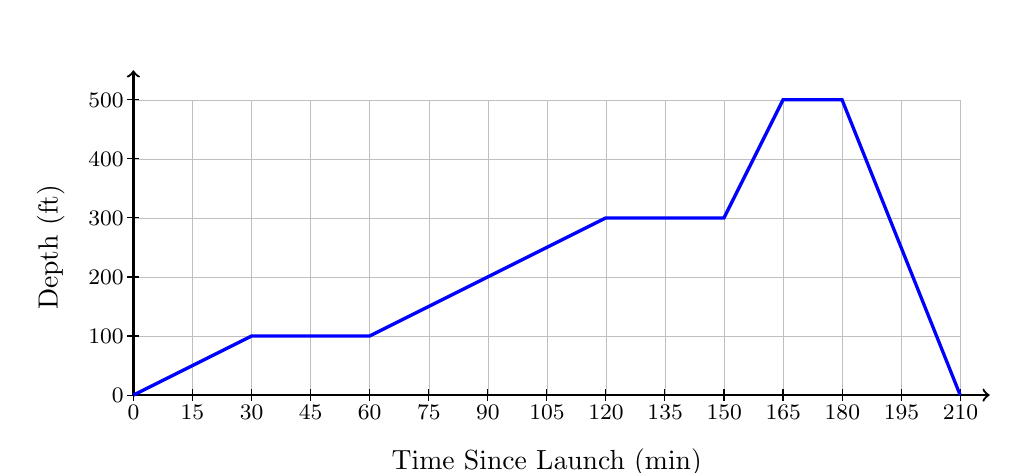
\begin{tikzpicture}[scale=0.75]
	\draw[ultra thin, gray!50] (0,0) grid (14,5);
	\draw[->,thick] (0,0) -- (14.5,0);
	\draw[->,thick] (0,0) -- (0,5.5);
	%% x-axis
	\foreach \x in {0,...,14}
		\draw (\x,0.1) -- (\x,-0.1);
	\foreach \x in {0,15,...,210}
		\draw (0.0667*\x, 0) node[below] {\footnotesize\x};
	\draw (7, -0.75) node[below] {Time Since Launch (min)};
	%% y-axis
	\foreach \y in {0,...,5}
		\draw (-0.1,\y) -- (0.1,\y);
	\foreach \y in {0,100,...,500}
		\draw (0, 0.01*\y) node[left] {\footnotesize\y};
	\draw (-1, 2.5) node[rotate=90,above] {Depth (ft)};
	%% graph
	\draw[very thick, blue] (0,0) -- (2,1) -- (4,1) -- (8,3) -- (10,3) -- (11,5) -- (12,5) -- (14,0);
\end{tikzpicture}
\end{center}
\end{boxedexplore}

At the beginning of the trip, Yeardleigh's submersible dives a total of 100 feet in the first 30 minutes. At the end of the trip, it returns to the surface, rising 500 feet in the last 30 minutes. This tells us that the depth of the submersible was \textit{changing much faster} at the end of the journey compared to the beginning.

Note that the graph reflects this: the line is quite steep at the end of the trip and not so steep at the beginning. The steeper the line, the faster the dependent variable is changing with respect to the independent variable.\footnote{We call this the ``rate of change'', and it will become an important focus of our work in \cref{ch:linear}.}

Plus, we can tell from the graph when the submersible is getting deeper (the depth is increasing; the line shows a positive trend) and when it is getting shallower (the depth is decreasing over time; the line shows a negative trend).

Notice that other parts of the graph are horizontal, for example between 30 and 60 minutes. This tells us that the depth of the submersible stayed the same during that time. Of course Yeardleigh could still be moving around below the surface, but she remains at a constant depth, neither diving nor surfacing.

\subsection{Interpreting curves}

Straight lines are fine, but what if the graph shows curved lines? Consider this graph showing the submersible's depth over time. What story would we tell about this graph?

%\resizeplot{0}{0}{100}{500}
%\begin{figure}
%\begin{tikzpicture}
%	\begin{axis}[
%		medsize,
%		defaultgrid,
%		labeloutsideaxis,
%		xlabel={Time (min)},
%		ylabel={Depth (ft)},
%	]
%	\addplot[samples=400, ultra thick, blue, domain=0:100](\x, -0.2*x^2+20*x);
%	\end{axis}
%\end{tikzpicture}
%\end{figure}

\begin{figure}
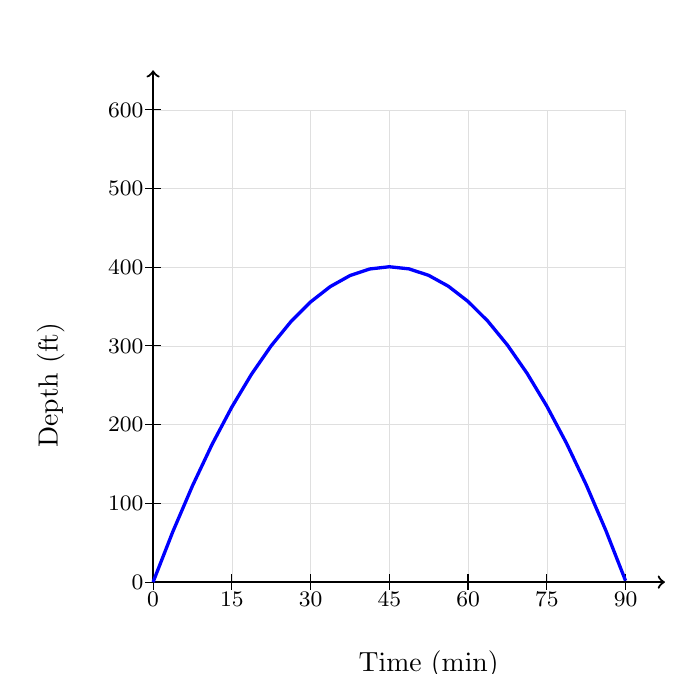
\begin{tikzpicture}[scale=1]
	\draw[ultra thin, gray!25] (0,0) grid (6,6);
	\draw[->,thick] (0,0) -- (6.5,0);
	\draw[->,thick] (0,0) -- (0,6.5);
	%% x-axis
	\foreach \x in {0,...,6}
		\draw (\x,0.1) -- (\x,-0.1);
	\foreach \x in {0,15,...,90}
		\draw (0.0667*\x, 0) node[below] {\footnotesize\x};
	\draw (3.5, -0.75) node[below] {Time (min)};
	%% y-axis
	\foreach \y in {0,...,6}
		\draw (0.1,\y) -- (-0.1,\y);
	\foreach \y in {0,100,...,600}
		\draw (0, 0.01*\y) node[left] {\footnotesize\y};
	\draw (-1, 2.5) node[rotate=90,above] {Depth (ft)};
	%% graph
	\draw[very thick, blue, domain=0:6] plot (\x,-0.444*\x*\x+2.667*\x);
\end{tikzpicture}
\end{figure}

One way to get a feel for what's happening is to imagine leaning a ruler or pencil against the rounded edge of a soda can. Then picture the ruler rolling along the side of the can, and how the angle of the ruler will change as it rolls.

\begin{figure}
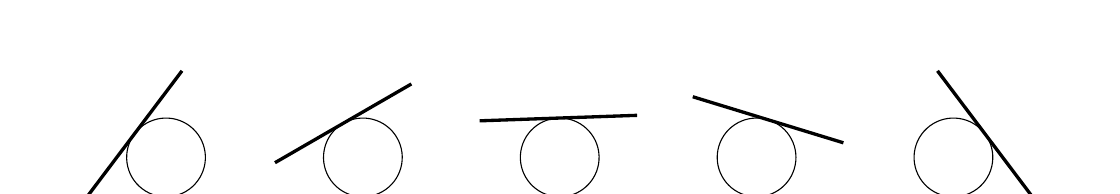
\begin{tikzpicture}[scale=0.5]
	\draw (-1.5,0) -- (25.5,0);
	\foreach \x in {-1,-0.75,...,25} \draw (\x,0) -- (\x-0.15, -0.25);
	\begin{scope}[rotate around={53:(2,1)}]
		\draw (2,1) circle[radius=1cm];
		\draw[very thick] (0,2) -- (4,2);
	\end{scope}
	\begin{scope}[xshift = 5cm, rotate around={30:(2,1)}]
		\draw (2,1) circle[radius=1cm];
		\draw[very thick] (0,2) -- (4,2);
	\end{scope}
	\begin{scope}[xshift = 10cm, rotate around={2:(2,1)}]
		\draw (2,1) circle[radius=1cm];
		\draw[very thick] (0,2) -- (4,2);
	\end{scope}
	\begin{scope}[xshift = 15cm, rotate around={-17:(2,1)}]
		\draw (2,1) circle[radius=1cm];
		\draw[very thick] (0,2) -- (4,2);
	\end{scope}
	\begin{scope}[xshift = 20cm, rotate around={-53:(2,1)}]
		\draw (2,1) circle[radius=1cm];
		\draw[very thick] (0,2) -- (4,2);
	\end{scope}
\end{tikzpicture}
\caption{Pencil rolling along the side of a can}
\end{figure}

Now picture a straight line rolling along the surface of the curved line in the graph above. The straight line approximates the curved line at the point where they touch.

\begin{figure}
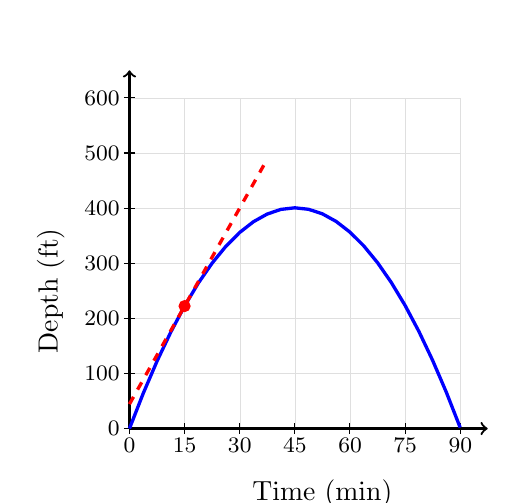
\begin{tikzpicture}[scale=0.7]
	\draw[ultra thin, gray!25] (0,0) grid (6,6);
	\draw[->,thick] (0,0) -- (6.5,0);
	\draw[->,thick] (0,0) -- (0,6.5);
	%% x-axis
	\foreach \x in {0,...,6}
		\draw (\x,0.1) -- (\x,-0.1);
	\foreach \x in {0,15,...,90}
		\draw (0.0667*\x, 0) node[below] {\footnotesize\x};
	\draw (3.5, -0.75) node[below] {Time (min)};
	%% y-axis
	\foreach \y in {0,...,6}
		\draw (-0.1,\y) -- (0.1,\y);
	\foreach \y in {0,100,...,600}
		\draw (0, 0.01*\y) node[left] {\footnotesize\y};
	\draw (-1, 2.5) node[rotate=90,above] {Depth (ft)};
	%% graph
	\draw[very thick, blue, domain=0:6] plot (\x,-0.444*\x*\x+2.667*\x);
	\draw[very thick, dashed, red, domain=0:2.5] plot (\x,1.778*\x+0.444);
	\draw[red,fill=red] (1,2.222) circle[radius=0.1];
\end{tikzpicture}
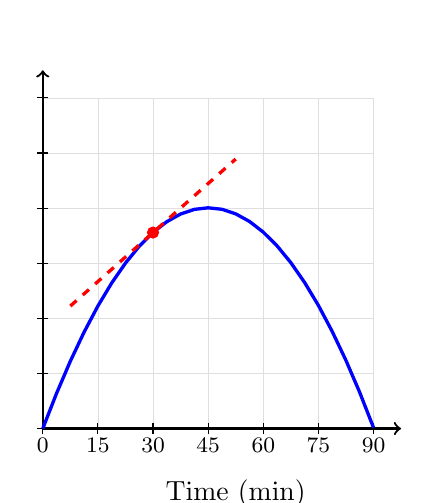
\begin{tikzpicture}[scale=0.7]
	\draw[ultra thin, gray!25] (0,0) grid (6,6);
	\draw[->,thick] (0,0) -- (6.5,0);
	\draw[->,thick] (0,0) -- (0,6.5);
	%% x-axis
	\foreach \x in {0,...,6}
		\draw (\x,0.1) -- (\x,-0.1);
	\foreach \x in {0,15,...,90}
		\draw (0.0667*\x, 0) node[below] {\footnotesize\x};
	\draw (3.5, -0.75) node[below] {Time (min)};
	%% y-axis
	\foreach \y in {0,...,6}
		\draw (-0.1,\y) -- (0.1,\y);
	%\foreach \y in {0,100,...,500}
	%	\draw (0, 0.01*\y) node[left] {\footnotesize\y};
	%\draw (-1, 2.5) node[rotate=90,above] {Depth (ft)};
	%% graph
	\draw[very thick, blue, domain=0:6] plot (\x,-0.444*\x*\x+2.667*\x);
	\draw[very thick, dashed, red, domain=0.5:3.5] plot (\x,0.889*\x+1.778);
	\draw[red,fill=red] (2,3.556) circle[radius=0.1];
\end{tikzpicture}
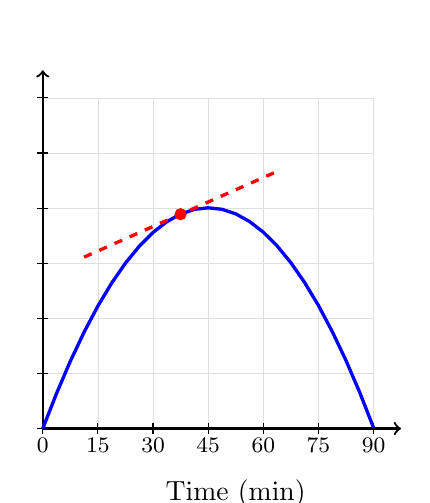
\begin{tikzpicture}[scale=0.7]
	\draw[ultra thin, gray!25] (0,0) grid (6,6);
	\draw[->,thick] (0,0) -- (6.5,0);
	\draw[->,thick] (0,0) -- (0,6.5);
	%% x-axis
	\foreach \x in {0,...,6}
		\draw (\x,0.1) -- (\x,-0.1);
	\foreach \x in {0,15,...,90}
		\draw (0.0667*\x, 0) node[below] {\footnotesize\x};
	\draw (3.5, -0.75) node[below] {Time (min)};
	%% y-axis
	\foreach \y in {0,...,6}
		\draw (-0.1,\y) -- (0.1,\y);
	%\foreach \y in {0,100,...,500}
	%	\draw (0, 0.01*\y) node[left] {\footnotesize\y};
	%\draw (-1, 2.5) node[rotate=90,above] {Depth (ft)};
	%% graph
	\draw[very thick, blue, domain=0:6] plot (\x,-0.444*\x*\x+2.667*\x);
	\draw[very thick, dashed, red, domain=0.75:4.25] plot (\x,0.444*\x+2.778);
	\draw[red,fill=red] (2.5,3.889) circle[radius=0.1];
\end{tikzpicture}
\end{figure}

Using the straight line, we can see that the submersible starts out diving at a fairly high rate. It gradually slows its rate of descent until it eventually stops diving. Then it gradually accelerates as it returns to the surface.\footnote{Believe it or not, this idea -- approximating a curved line with a straight line -- is one of the fundamental motivating ideas in calculus. As you work to interpret these curved graphs, you're growing your calculus brain, right here in Algebra 1. How cool is that?}

\subsection{Impossible situations}

Consider this graph showing the submersible's depth over time. What's going on here?

\begin{figure}
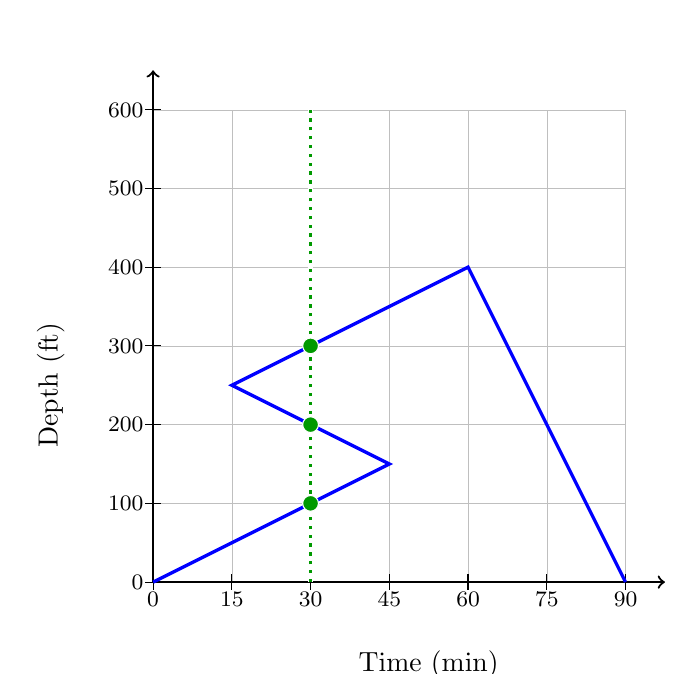
\begin{tikzpicture}[scale=1]
	\draw[ultra thin, gray!50] (0,0) grid (6,6);
	\draw[->,thick] (0,0) -- (6.5,0);
	\draw[->,thick] (0,0) -- (0,6.5);
	%% x-axis
	\foreach \x in {0,...,6}
		\draw (\x,0.1) -- (\x,-0.1);
	\foreach \x in {0,15,...,90}
		\draw (0.0667*\x, 0) node[below] {\footnotesize\x};
	\draw (3.5, -0.75) node[below] {Time (min)};
	%% y-axis
	\foreach \y in {0,...,6}
		\draw (-0.1,\y) -- (0.1,\y);
	\foreach \y in {0,100,...,600}
		\draw (0, 0.01*\y) node[left] {\footnotesize\y};
	\draw (-1, 2.5) node[rotate=90,above] {Depth (ft)};
	%% graph
	\draw[very thick, blue] (0,0) -- (3,1.5) -- (1,2.5) -- (4,4) -- (6,0);
	\draw[ultra thick, white] (2,0) -- (2,6);
	\draw[very thick, dotted, green!60!black] (2,0) -- (2,6);
	\draw[white,fill=green!60!black] (2,1) circle[radius=0.1];
	\draw[white,fill=green!60!black] (2,2) circle[radius=0.1];
	\draw[white,fill=green!60!black] (2,3) circle[radius=0.1];
\end{tikzpicture}
\end{figure}

This graph is a problem, given the context of ``depth of the submersible over time''. Consider this question: How deep it the submersible 30 minutes after launch?

According to the graph, the submersible is 100 feet deep\ldots\ and 200 feet deep\ldots\ \textit{and} 300 feet deep\ldots\ all at the same time! That's impossible!

This kind of problem could pop up in other places. For example, in a distance-time graph, points that line up vertically mean that something is in more than one place at one instant in time. Though we might wish reality were different, nothing can be in two (or more) places at the same time.

Graphs like this -- where several $y$-values stack up vertically over the same $x$-value -- violate a certain requirement that we will learn about in the next chapter, as we delve into the important mathematical idea of a \textit{function}.

% % % % % % % % % % % % % % % % % % % % % % % % % % % % % % % % % % % % % % % % 
\chaptersummary

In this chapter we began with plotting points to create the graph of a sequence. Then, we built upon these ideas to create the graph of function. We then turned our attention from making graphs to understanding graphs that are given to us.

These two skills -- creating a graph from a given rule, and extracting information from a given graph -- are both key mathematical skills that we will develop in this course. At the heart of both skills lies the connection between a function's rule and its graph. This connection, and more about the concept of a function, is the focus of the next chapter. Onward!
\chapter{Fundamentals of functions}
\label{ch:functions}

%A mathematician is a machine for turning coffee into theorems.
%\par\hfill --- Paul Erd\H{o}s, Hungarian mathematician

\chapquote{On two occasions I have been asked, ``Pray, Mr. Babbage, if you put into the machine wrong figures, will the right answers come out?'' I am not able rightly to apprehend the kind of confusion of ideas that could provoke such a question.}{Charles Babbage, English inventor of the first mechanical computer}

We have seen a number of relationships so far: the relationship between distance and time of a moving object, for example, or the relationship between a number's position in a sequence and that number's value. A \textit{function} is a certain kind of relationship that is of key importance to us in algebra, and indeed throughout mathematics. In this chapter we'll get an overview of functions and their different representations. then, in the rest of the course, we will look closely at three specific kinds of functions.

% % % % % % % % % % % % % % % % % % % % % % % % % % % % % % % % % % % % % % % % 
\section{Mathematical relationships}
\label{sec:mathrelationships}

%\begin{boxexplore}[Name of Extended Exploration]
%\addtodoitem{Click here to visit the extended exploration: NAME}
%\end{boxexplore}

\begin{boxexplore}[Number machines]
A number machine accepts numbers as input and produces numbers as output. When machine A receives the number 8 as input, it produces the output 28. When this machine receives $\umin12$ as input, the output is $\umin42$.

Machine B has a different mechanism for producing output values. When machine B receives the number 8 as input, it outputs 15. When it receives $\umin12$ as input, the output is $23$.

What do you suppose each machine will output when given the number $\umin7$ as input? Write a sentence explaining how you believe each machine works.
\end{boxexplore} %% End of startup exploration

The number machines described in the startup exploration relate certain input values to certain output values. Mathematically speaking, a number machine defines a \textit{relation}.

\begin{boxdef}[Relation]
A \gls{relation} defines how certain numbers (or other objects) are connected to other numbers (or objects). We can think of a relation as a collection of ordered pairs $(x,y)$, meaning ``$x$ is related to $y$''.
\end{boxdef}

We might think of a number machine as a set of pairs of numbers: (input, output). Machine A in the startup exploration is defined by the pairs $(8, 28)$ and $(-12, -42)$. We sometimes say that ``machine A maps 8 to 28'' and that ``-12 is mapped to -42''.

One possible explanation is that the machine multiplies the input value by 3.5 to produce the output value. In this case, we'd expect the input $-7$ to produce the output $-24.5$. In other words, $(-7, -24.5)$ is a third point associated with machine A.

For machine B we are given the points $(8, 15)$ and $(-12, 23)$. One, somewhat complicated, explanation is that the machine doubles the input, takes the absolute value of the result, and then subtracts 1. In this case, we'd have $(-7, 13)$ as another input-output pair for machine B.\footnote{There are other rules that we could write based on the two data points we were given, and perhaps you thought of different rules than the ones we describe here. Can you find alternative explanations for how each machine works? Be creative!}

We can define relations that compare things other than numbers. For example, we might define the ``name-the-mother'' relation that accepts a person as input and which gives that person's biological mother as output. Or, we might define the ``name-the-pet'' relation, which accepts a human as input and outputs other animals.

Note that there is a difference between these two relations we have just defined. Not all people own pets, so some inputs to the name-the-pet macine have no output. Plus, some people own multiple pets, so some inputs to the name-the-pet machine have multiple outputs. On the other hand, the name-the-mother machine is guaranteed to always produce a unique output: every person has a biological mother, and every person has exactly one biological mother. It is impossible for someone to have more than one biological mother!\footnote{We don't deny that a family with two mothers is still a family! It is true that a person can have multiple mothers in a legal or emotional sense\ldots\ but a person has exactly one \textit{biological} mother.}

We saw something similar in \cref{sec:interpgraphs}, where certain graphs could be drawn in a way that would suggest an impossible situation. For example, we drew a graph (shown in \cref{fig:impossible}) that suggested Yeardleigh's submersible could at three different depths simultaneously, which -- like have more than one biological mother -- is nonsense.
%\footnote{``I like nonsense; it wakes up the brain cells.'' --- Dr. Seuss}

\begin{figure}[!htbp]
\centering
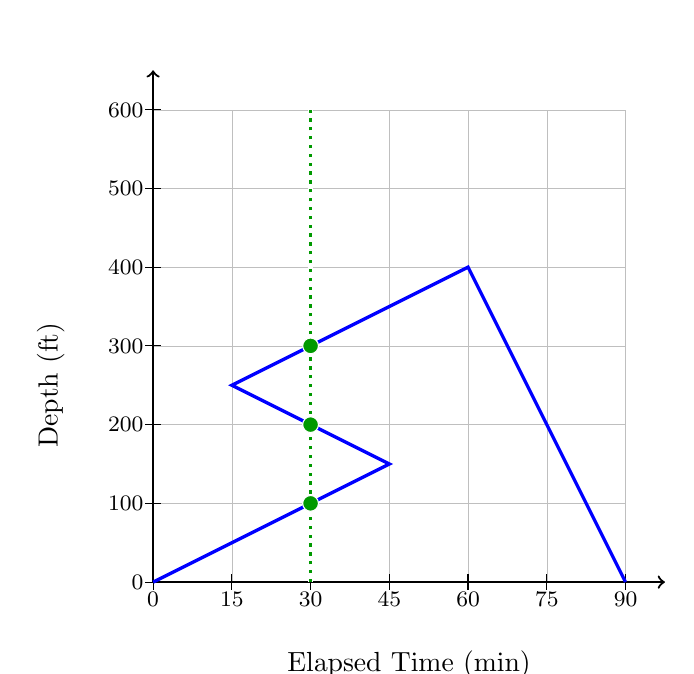
\begin{tikzpicture}[scale=1]
	\draw[ultra thin, gray!50] (0,0) grid (6,6);
	\draw[->,thick] (0,0) -- (6.5,0);
	\draw[->,thick] (0,0) -- (0,6.5);
	%% x-axis
	\foreach \x in {0,...,6}
		\draw (\x,0.1) -- (\x,-0.1);
	\foreach \x in {0,15,...,90}
		\draw (0.0667*\x, 0) node[below] {\footnotesize\x};
	\draw (3.25, -0.75) node[below] {Elapsed Time (min)};
	%% y-axis
	\foreach \y in {0,...,6}
		\draw (-0.1,\y) -- (0.1,\y);
	\foreach \y in {0,100,...,600}
		\draw (0, 0.01*\y) node[left] {\footnotesize\y};
	\draw (-1, 2.5) node[rotate=90,above] {Depth (ft)};
	%% graph
	\draw[very thick, blue] (0,0) -- (3,1.5) -- (1,2.5) -- (4,4) -- (6,0);
	\draw[ultra thick, white] (2,0) -- (2,6);
	\draw[very thick, dotted, green!60!black] (2,0) -- (2,6);
	\draw[white,fill=green!60!black] (2,1) circle[radius=0.1];
	\draw[white,fill=green!60!black] (2,2) circle[radius=0.1];
	\draw[white,fill=green!60!black] (2,3) circle[radius=0.1];
\end{tikzpicture}
	\caption{A graph of depth over time? Impossible!}
	\label{fig:impossible}
\end{figure}

Relationships that follow this very natural rule -- any given input produces a unique output -- have a special status in algebra. They're called \glspl{function}.

%From a certain point of view, there is nothing wrong with this graph --- any old squiggly line in the coordinate plane is a kind of graph. The problem arises because this graph doesn't make any sense \textit{in the context of the problem}. In this chapter, we will make some formal definitions that will help us to distinguish certain types of mathematical rules and relationships from one another.

\begin{boxdef}[Function]
A \gls{function} is a special type of relation in which the ordered pairs have the following property: each $x$-value is paired with one, and only one, $y$-value.
\end{boxdef}

The ``one and only one'' requirement is what makes a function special. The graph in \cref{fig:impossible} violates this requirement: certain $x$-values have more than one associated $y$-value (look at $x$ values between 15 and 45 minutes). So, this graph does not depict a function. Any given sequence is a function, since each $x$ value (position in the sequence) is occupied by exactly one $y$ value.

A sequence is a function: it would be silly to suggest that a sequence had more than one value as its third term. Depending on how we think about number machines, we might expect that a machine would act predictably and always produce the same output for a given input. A number machine that behaves in this way defines a function.

\subsubsection{Representing relations}

Ther are several ways to represent a mathematical relation. We might represent a relation using:
\begin{itemize}
\item A graph. This representation gives us a visual of the relationship between input values and output values.
\item A table of values. This representation gives us an organized list of input values and their corresponding output values. (Related forms include a \textit{mapping diagram}, or just a collection of ordered pairs.)
\item An equation. This representation gives us a rule for turning input values into output values, the way a number machine might do.
%-- A mapping diagram. Like a table, gives a series of input and corresponding output values.
%-- A set of points. Like a table, but organized differently
\end{itemize}

Since functions hold a special position in the universe of all relations, our first task is to determine whether a given mathematical relationship is, in fact, a function. To do this we have to check it against the definition of what it means to be a function. In other words, we must make sure each $x$-value corresponds to one and only one $y$-value.

%There are different features we can look for depending on the representation of the function, but the key question is always the same: does every $x$ correspond to a unique $y$?

\subsection{Graphs of functions}

In order for a graph to be a function it must avoid the situation in which multiple $y$-values stack up above a particular $x$-value. A handy way of remembering this requirement is that the graph of a function passes the \gls{vertical line test}. The vertical line test states that for the graph of a function, any vertical line drawn on the graph will intersect the graph \textit{exactly once}.

\begin{boxex}
Which of the graphs below, if any, represents a function? How do you know?

% Graph 1
\begin{minipage}{0.33\textwidth}
\centering
Graph A
\par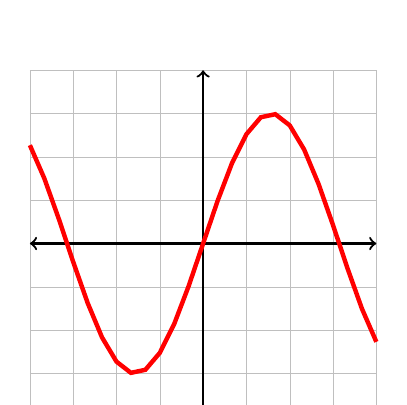
\begin{tikzpicture}[scale=0.55]
	\draw[ultra thin, gray!50] (-4,-4) grid (4,4);
	\draw[<->,thick] (-4,0) -- (4,0);
	\draw[<->,thick] (0,-4) -- (0,4);
%	\draw (0, 4.75) node {Graph A};
	%% graph
	\draw[ultra thick, red, domain=-4:4] plot (\x, {3*sin(\x r)});
\end{tikzpicture}
\end{minipage}
% Graph 2
\begin{minipage}{0.33\textwidth}
\centering
Graph B
\par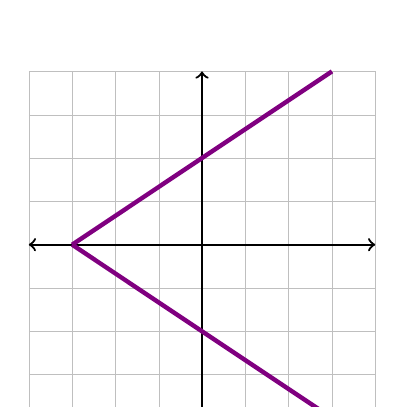
\begin{tikzpicture}[scale=0.55]
	\draw[ultra thin, gray!50] (-4,-4) grid (4,4);
	\draw[<->,thick] (-4,0) -- (4,0);
	\draw[<->,thick] (0,-4) -- (0,4);
%	\draw (0, 4.75) node {Graph B};
	%% graph
	\draw[ultra thick, violet, domain=-3:3] plot (\x,0.667*\x+2);
	\draw[ultra thick, violet, domain=-3:3] plot (\x,-0.667*\x-2);
\end{tikzpicture}
\end{minipage}
% Graph 3
\begin{minipage}{0.33\textwidth}
\centering
Graph C
\par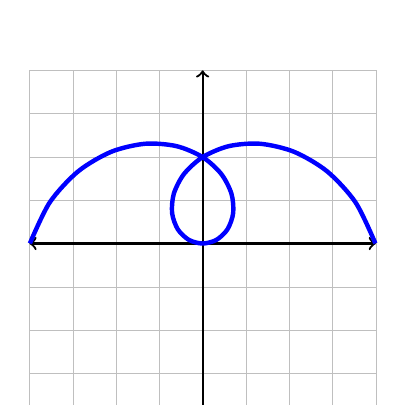
\begin{tikzpicture}[scale=0.55]
	\draw[ultra thin, gray!50] (-4,-4) grid (4,4);
	\draw[<->,thick] (-4,0) -- (4,0);
	\draw[<->,thick] (0,-4) -- (0,4);
%	\draw (0, 4.75) node {Graph C};
	%% graph
	%\draw[ultra thick, blue] (0,0) circle[radius=3cm];
	\draw[ultra thick, blue, scale=1.27,domain=-3.141:3.141,smooth,variable=\t] plot ({\t*cos(\t r)},{\t*sin(\t r)});
\end{tikzpicture}
\end{minipage}

\exsoln\ Only graph A represents a function. We can draw vertical lines on graphs B and C which intersect the graph at more than one point. This means that those $x$-values have more than one $y$-value, violating the definition of function.
\end{boxex}

Note that in graph C, certain sections of the graph pass the vertical line test. There is no partial credit, though. A graph fails the vertical line test if any vertical line (even just one) crosses the graph in more than one point. This happens also with the graph in \cref{fig:impossible}. That graph fails the vertical line test for some vertical lines. Therefore the relationship depicted is not a function.

\begin{boxex}
Which of the scatter plots below, if any, represents a function? How do you know? You may have to look closely!

% Graph 1
\begin{minipage}{0.33\textwidth}
\centering
Plot A
\par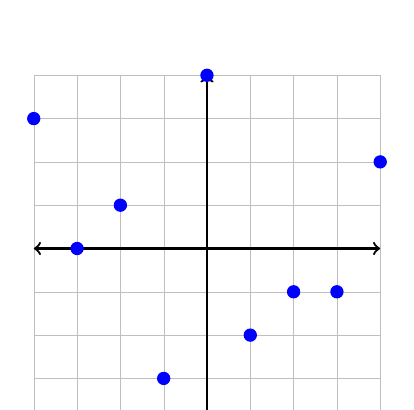
\begin{tikzpicture}[scale=0.55]
	\draw[ultra thin, gray!50] (-4,-4) grid (4,4);
	\draw[<->,thick] (-4,0) -- (4,0);
	\draw[<->,thick] (0,-4) -- (0,4);
%	\draw (0, 4.75) node {Plot A};
	%% graph
	\draw[blue] plot[only marks, mark=*, mark size=4] coordinates {(-4,3) (-3,0) (-2,1) (-1,-3) (0,4) (1,-2) (2,-1) (3,-1) (4,2)};
\end{tikzpicture}
\end{minipage}
% Graph 2
\begin{minipage}{0.33\textwidth}
\centering
Plot B
\par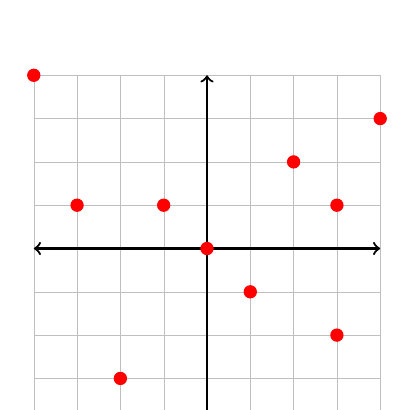
\begin{tikzpicture}[scale=0.55]
	\draw[ultra thin, gray!50] (-4,-4) grid (4,4);
	\draw[<->,thick] (-4,0) -- (4,0);
	\draw[<->,thick] (0,-4) -- (0,4);
%	\draw (0, 4.75) node {Plot B};
	%% graph
	\draw[red] plot[only marks, mark=*, mark size=4] coordinates {(-4,4) (-3,1) (-2,-3) (-1,1) (0,0) (1,-1) (2,2) (3,1) (3,-2) (4,3)};
\end{tikzpicture}
\end{minipage}
% Graph 3
\begin{minipage}{0.33\textwidth}
\centering
Plot C
\par\begin{tikzpicture}[scale=0.55]
	\draw[ultra thin, gray!50] (-4,-4) grid (4,4);
	\draw[<->,thick] (-4,0) -- (4,0);
	\draw[<->,thick] (0,-4) -- (0,4);
	%% graph
	\draw[green!80!black] plot[only marks, mark=*, mark size=4] coordinates {(-4,1) (-3,1) (-2,1) (-1,1) (0,1) (1,1) (2,1) (3,1) (4,1)};
\end{tikzpicture}
\end{minipage}

\exsoln\ Plots A and C both pass the vertical line test, and therefore represent functions. Plot B fails the vertical line test because it fails for the vertical line at $x=3$.
\end{boxex}

Note that we don't care if different $x$'s map to the same $y$. For example, in plot C, all of the $x$-values map to the same $y$-value. That's OK. In other words, a function \textit{can} fail the ``horizontal line test'' without penalty.\footnote{The horizontal line test \textit{is} a thing, and passing or failing the horizontal line test does have a mathematical meaning. But, a discussion of this will have to wait until later.}

For example, the name-the-mother function does not pass the horizontal line test because two different inputs (people) can have the same output (mother). In fact, it is not at all uncommon for two different people to have the same mother: they're called siblings!

\subsection{Functions from points}

A scatter plot gives a visual representation of a collection of ordered pairs. If the ordered pairs are presented in an alternative format -- say, a table of values -- we can use the same reasoning to determine whether the given relation is a function.

\begin{boxex}
Which of the data sets below, if any, represents a function? How do you know?

\begin{minipage}[t]{0.33\textwidth}
\centering
Set A
\par\begin{tabular}{|C{1.5cm}|C{1.5cm}|}
\hline
x & y \\\hline
-3 & 4\\
-2 & 6\\
-1 & 4\\
0 & 2\\
1 & 0\\
2 & -2\\
3 & 0\\\hline
\end{tabular}
\end{minipage}
% Graph 2
\begin{minipage}[t]{0.33\textwidth}
\centering
Set B
\par\begin{tabular}{|C{1.5cm}|C{1.5cm}|}
\hline
x & y \\\hline
2 & 1\\
1 & 2\\
-1 & 7\\
4 & 3\\
3 & 4\\
1 & 0\\
0 & 6\\\hline
\end{tabular}
\end{minipage}
% Graph 3
\begin{minipage}[t]{0.33\textwidth}
\centering
Set C
\par
\[\left\{\begin{array}{ll}
(0,4); &(-1,6);\\
(2,3); &(0,4);\\
(1,5); &(-2,5)
\end{array}\right\}\]
\end{minipage}

\exsoln\ Set A is a function. There are no repeated $x$-values! Set B is not a function. The $x$-value 1 appears twice and with two different related $y$-values (0 and 2). This violates the definition of function. Set C is a function. The $x$ value 0 appears twice, but it is mapped to the same value in both cases.
\end{boxex}

A \gls{mapping diagram} is a similar way of representing a relationship between specific input and output values. Here we draw two regions (represented by a box or an oval). In one region, we list the input values, in the other region we list the output values. Then we draw arrows to show which input maps to which output.

\begin{boxex}
Which of the mapping diagrams below, if any, represents a function? How do you know?

\begin{minipage}{0.5\textwidth}
\centering
Diagram A
\par\begin{tikzpicture}[scale=0.55]
	\draw (0,0) circle[x radius=1.5, y radius=3];
	\draw (5,0) circle[x radius=1.5, y radius=3];
	\draw (0, 1.5) node[left]{1};
	\draw (0, 0.5) node[left]{2};
	\draw (0, -0.5) node[left]{3};
	\draw (0, -1.5) node[left]{4};
	\draw (5, 1.5) node[right]{2};
	\draw (5, 0.5) node[right]{6};
	\draw (5, -0.5) node[right]{9};
	\draw (5, -1.5) node[right]{0};
	\draw[thick,->] (0,1.5) -- (5,1.5);
	\draw[thick,->] (0,0.5) -- (5,-1.5);
	\draw[thick,->] (0,-0.5) -- (5,0.5);
	\draw[thick,->] (0,-1.5) -- (5,-0.5);
\end{tikzpicture}
\end{minipage}
% Graph 2
\begin{minipage}{0.5\textwidth}
\centering
Diagram B
\par\begin{tikzpicture}[scale=0.55]
	\draw (0,0) circle[x radius=1.5, y radius=3];
	\draw (5,0) circle[x radius=1.5, y radius=3];
	\draw (0, 1.5) node[left]{1};
	\draw (0, 0.5) node[left]{2};
	\draw (0, -0.5) node[left]{3};
	\draw (0, -1.5) node[left]{4};
	\draw (5, 1) node[right]{9};
	\draw (5, -1) node[right]{7};
	\draw[thick,->] (0,1.5) -- (5,-0.8);
	\draw[thick,->] (0,0.5) -- (5,1.1);
	\draw[thick,->] (0,0.5) -- (5,-1);
	\draw[thick,->] (0,-0.5) -- (5,0.9);
	\draw[thick,->] (0,-1.5) -- (5,-1.2);
\end{tikzpicture}
\end{minipage}

\exsoln\ The first mapping is a function. Each $x$-value maps to exactly one $y$-value. The second mapping is not a function: the value 2 maps to both 7 and 9.
\end{boxex}

Note again that the problem in diagram 2 is \textit{not} that multiple arrows point to each of the output numbers. It's OK for multiple arrows to go \textit{toward} a certain output value. The problem is that the input value 2 has multiple arrows \textit{leaving} and going to different targets (both 7 and 9).

%The table, the mapping diagram, and the list of points are all basically the same sort of representation: we are presented with a finite number of ordered pairs. So, these representations only give a limited picture of how the function operates. The preferred representations are the graph and the equation.

% If you are given one of the others, you will likely have to convert it to a graph or an equation.

\subsection{Equations of functions}

The ``number machine'' metaphor is often helpful when thinking about a function. A number (an $x$-value) goes into the machine, the machine's rule works on the number, and another number comes out of the machine (the $y$-value). Most of the time, when we have a particular rule and a particular input, we get a single, predictable output.

For example, the equation $y = 3x$ defines a function. We can substitute in 5 for $x$. The function machine multiplies 5 by 3 and outputs 15. This generates the ordered pair $(5, 15)$ and we say that ``5 maps to 15''. If we choose other values of $x$, we can generate more ordered pairs.

Not every equation defines a function, though. In order to be a function, every input value must produce one and only one output value. In Algebra 2 we will study many interesting and important mathematical relationships that are not functions. We will learn, for instance, how to write the equation for a circle -- and a circle is not a function. (Can you explain why not?)

Our focus in Algebra 1, though, will be on three main ``families'' of functions, and our rules will all be of the form ``$y$ equals some expression in terms of $x$''.

%In addition to being able to determine if a relation is a function, one has to be able to convert between the different representations. We will spend more time on this when we study each family of functions in depth.

\subsection{Function notation}

%\begin{boxexplore}[Name of Extended Exploration]
%\addtodoitem{Click here to visit the extended exploration: NAME}
%\end{boxexplore}

%\begin{boxexplore}[Name of Startup Exploration]
%Description of startup exploration.
%\end{boxexplore} %% End of startup exploration
\addtodoitem{Startup exploration on function notation?}

We can thank Swiss mathematician Leonhard Euler for the concept of a function.\footnote{The surname Euler is German, and so it is pronounced $OIL \cdot er$ (and \textit{not} $YOO \cdot ler$).} He was the first to coin the term ``function'' and was the first to use a handy way of writing a function, called \textit{function notation}.

Up until now, we have used ``$y=$ something in terms of $x$'' to define all of our rules. Euler's function notation looks a bit different, but it is quite helpful in certain situations. The generic form of function notation is ``$f(x)~=$ something in terms of $x$''. In this case, we simply replace $y$ with the notation $f(x)$, which is read aloud as ``$f$ of $x$'' or ``$f$ as a function of $x$''.

In its generic form, the letter $f$ is used to name the function. We use the letter $f$, of course, because it stands for ``function''. And as usual, we use $x$ to represent the independent variable.

What's nice about this notation is that it allows us great flexibility to use other letters or symbols that can be more descriptive. For example, if we wanted to describe how the height of a bouncing ball changes over time, we might want to let the variable $t$ represent time, and then name the function $h$ for height.

So, we could write a function ``$h(t) =$ some expression in terms of $t$''. That's read ``$h$ of $t$'', which does a pretty good job of capturing the idea that we're describing \textit{height} in terms \textit{of time}.

We might write a function like $d(t) = 60t$ which described distance traveled $d$ as a function of time $t$. This is exactly the same equation as $y = 60x$, but we've changed the names of things to better match the context.

\subsubsection{Evaluation using function notation}

Function notation has another convenience. We can use the notation to indicate a specific choice of value for the independent variable. Earlier, we said: ``Evaluate the function $y = x^2-4$ when $x = 3$.'' This was fine, but function notation gives us a way to shorten these instructions.

For example, if we have $f(x) = x^2-4$ then we might want to evaluate $f(3)$, which is said aloud ``$f$ of three''. The $x$ in the function notation was replaced by 3, which is exactly what is means to evaluate the function at that value! The notation is telling us to input 3 for $x$ and find the output value. So if $f(x) = x^2 - 4$, then \[f(3) = (3)^2 - 4 = 9 - 4 = 5.\]

We will use function notation and $y =$ notation through this course. The flexibility of function notation means that it is the preferred way of writing functions in higher level mathematics courses.


% % % % % % % % % % % % % % % % % % % % % % % % % % % % % % % % % % % % % % % 
\section{Domain and range}
\label{cref:domandrange}

\addtodoitem{More examples here: see Patty's notes.}

%\begin{boxexplore}[Name of Extended Exploration]
%\addtodoitem{Click here to visit the extended exploration: NAME}
%\end{boxexplore}

Machines (meaning real, mechanical devices) are physical things that have physical limitations. Number machines (meaning functions) often have similar operational restrictions.

\begin{boxexplore}[The ins and outs of functions]
Consider the function machines below.
\[f(x) = \abs{x} \qquad\qquad g(x)=\frac{1}{x}\]
% \qquad\qquad h(x)=\frac{3}{x-2}\]
What sorts of values are allowed as input to each of these machines? What sorts of values will each one produce as output?
\end{boxexplore} %% End of startup exploration

A blender is a machine that has limited operating parameters. Anything we put into the blender comes out ``blended'' in some way. But, of course, there are some things we can't put in a blender: a piano, for example.\footnote{We'll pause here to note that ``blended'' is defined rather loosely: smoothies come out ``blended'', ice comes out ``crushed'', chickpeas come out ``pur\'eed'', magazines come out ``shredded''\ldots\ We consider all of these to be a kind of ``blended''. Speaking of magazines, we'll also mention that there are things which one \textit{can} put into a blender, but \textit{shouldn't}. Magazines are one example. Another example: your hand.} Similarly, we wouldn't put bread into a  blender, hit the button, and expect toast to pop out. That kind of output is associated with a different machine.

\subsection{Regarding input values}

An important component of the definition of any function is a specification about what sorts of numbers it can accept as input. In the language of mathematics, we call the set of all ``legal'' input values the \textit{domain} of the function.

\begin{boxdef}[Domain]
The set of all allowed input values to a function. This is the set of all allowed $x$-values, or all possible values of the independent variable.
\end{boxdef}

We have two functions in the startup exploration. The first function, $f(x)=\abs{x}$, is very welcoming: any real number can be used as unput to this number machine: whole numbers, fractions, positive numbers, negative numbers, it doesn't matter. The other function is a little more finicky.

In \cref{ch:numbers}, we discussed the illegality of division by zero. So, if we try to put 0 into the function $g(x)=\frac{1}{x}$, then we're going to have a problem: $g(0)$ -- that's the function $g$ evaluated at $x=0$ -- is undefined. So, our user manual for the function $g$ has to include a note that only numbers other than 0 are allowed as input. We say that the function $g(x)$ has a \textit{limited} or \textit{restricted domain}.

%%%What does this mean for the function $h(x) = \frac{3}{x-2}$, which also has $x$ in its denominator? In this case, $h(0)$ is no problem:
%%%\[h(0) = \frac{3}{0-2} = \frac{3}{-2} = -\frac{3}{2}.\]
%%%The problem in this case is when $x=2$, for then the denominator is $2-2=0$. So, $h$ has the restriction that only numbers other than 2 are allowed as input.
%%%
%%%\subsubsection{Limited domains}
%%%
%%%We say that the function $g(x)$ has a \textit{limited} or \textit{restricted domain}. 
%%%There are certain values that cannot be allowed as input because the function would ``break''.
%%%
%%%Another function with a limited domain is the square-root function $y = \sqrt{x}$. This function can only accept nonzero numbers as input. All negative numbers are restricted from the domain.\footnote{Try to take the square root of a negative number on a calculator and see what happens! Stay tuned for more on this phenomenon, and other stuff about square roots, in \cref{ch:radicals}.}

There are other circumstances where we will want or need to limit the domain. For example, a domain can be limited by the context of a problem we are solving. If we write an equation that shows distance as a function of time, it usually makes sense to limit the domain to only include positive time-values. If we have a function which maps ``number of pizza toppings'' to ``price of the pizza'', then there is (probably) an upper limit on the domain: there are only so many pizzas toppings available.\footnote{Did you know that the so-called ``Hawaiian pizza'', a pizza topped with pieces of ham and pineapple, is not actually a Hawaiian invention? Several news organizations agree that this pizza originated in Ontario, Canada.}

A sequence is a function whose domain is limited to the set of natural numbers (the positive integers). We saw this in \cref{ch:sequences,,ch:graphs}: a sequence can have a first term and a second term, but no one-and-a-halfth term. We exclude from the domain of a sequence all numbers except $1, 2, 3, 4, \dotsc$.

We can also define a specific domain for convenience. On an assignment, for example, we might be asked to evaluate the function $y=4x+5$ for the $x$-vales $-1$, 0, and 1. We did something like this in \cref{ex:evaluating}. This is another example of limiting the domain.

%%%The three families of functions that we will study most closely in Algebra 1 (the linear, exponential, and quadratic families) do not require any domain restrictions, which is good news.

\subsection{Regarding output values}

In addition to knowing about input values, it is often important for us to know what sorts of numbers we can expect as output from a certain function. We call the set of all output values the \textit{range} of the function.

\begin{boxdef}[Range]
The set of all output values from a function. This is the set of all $y$-values, or all possible values of the dependent variable.
\end{boxdef}

The function $f(x) = \abs{x}$ can accept any number as input, but only non-negative numbers ever come out. We say that the range of $f$ is non-negative real numbers.

In the case of $g(x) = \frac{1}{x}$, notice that the only way for a fraction to equal 0 is if the numerator is equal to zero. No matter what nonzero input value we put into the function $g$, we will never get 0 as the output! The range of $g$ is nonzero real numbers.

%%%This is also true of $h(x) = \frac{3}{x-2}$. No matter what (legal) value of $x$ we choose, $h(x)$ will never be 0. This function to has range of nonzero real numbers.

\subsubsection{Piecewise definition}

An interesting way to control the output of a function is to give it different definitions depending on the input. For example, suppose we define a function like so:
\begin{equation*}
f(x) = \begin{cases}
~x	& \text{if $x$ is positive}
\\
-x	& \text{if $x$ is negative}
\\
~0	& \text{if $x$ is equal to 0}
\end{cases}
\end{equation*}
This unusual notation gives us several definitions at once, depending on which of the ``if'' statements applies to a given input value $x$.

If the input $x$ is positive, then the output is simply $x$ itself. If the input is negative, then the output is the opposite of $x$ (so again, we get a positive value). Finally, in the third case, if the input is 0, then we get 0 as the output. Do you recognize this function? This case-by-case definition is really just a complicated way of saying $f(x) = \abs{x}$.

Here's a more interesting example. Suppose we define a function whose domain is the non-negative integers as follows:
\begin{equation*}
z(n) = \begin{cases}
~~\dfrac{~n~}{2} & \text{if $n$ is even}
\\[3ex]
-\dfrac{n+1}{2} & \text{if $n$ is odd}
\end{cases}
\end{equation*}
This function produces different output depending on whether the input value is even or odd. Let's try the first few input values to see what happens. What happens when we input 0? Zero is an even number, so the first case applies and:
\[z(0) = \frac{0}{2} = 0.\]
One is an odd number, so the second case applies:
\[z(1) = -\frac{1+1}{2} = -\frac{2}{2} = -1\]
Two is even, and three is odd. So we have:
\[z(2) = \frac{2}{2} = 1 \qquad\text{and}\qquad z(3) = -\frac{3+1}{2} = -\frac{4}{2} = -2.\]
This function produces the sequence:
\[0, -1, ~1, -2, ~2, -3, ~3, -4, ~4,\cdots\]
which is a list of all the integers. In other words: this machine turns the natural numbers $\N$ (plus zero) into the set of integers $\Z$.\footnote{This function suggests a shocking idea. Most people would say that there are more integers than there are natural numbers. After all, since the integers include all of the natural numbers \textit{and} all of the opposites of the natural numbers, it must be that the set of integers has \textit{twice as many members}\ldots\ right? Nope! The set of natural numbers and the set of integers are \textit{exactly the same size}. Think of it this way: the function $z$ defined above pairs up natural numbers and integers. If I give you a natural number (input), can you tell me what integer (output) it partners up with? If I give you an integer (output), can you tell me what natural number (input) it partners up with? If so, then the two sets match up exactly and neither set has any leftovers. They must therefore be the same size! Mind blown!}

%%%
%%%\subsection{Domain and range from tables and graphs}
%%%
%%%\begin{boxex}
%%%Consider the table of values below. Does this table represent a function? If so, what are the domain and range given?
%%%
%%%\begin{center}
%%%\begin{tabular}{|C{2cm}|C{2cm}|}
%%%\hline
%%%x	& y\\\hline
%%%5	& 14\\
%%%6	& 17\\
%%%7	& 20\\
%%%8	& 23\\\hline
%%%\end{tabular}
%%%\end{center}
%%%
%%%\exsoln\ Based on the table, we do have a function since no $x$-values are repeated. To state the domain and range from a tabular representation, we just list the values in set notation. The domain is $x \in \{5, 6, 7, 8\}$, and the range is $y \in \{14, 17, 20, 23\}$.
%%%\end{boxex}
%%%
%%% JASON SAYS NO
%%%
%%%When given a portion of a graph and asked to find domain and range, the key is to look at maximum and minimum values. Consider the below, showing a piece of a function. What can we say about its domain and range?
%%%
%%%\resizeplot{-8}{-8}{8}{8}
%%%\begin{figure}
%%%\begin{tikzpicture}
%%%	\begin{axis}[standard]
%%%		\draw[very thick, blue] (axis cs: -4,5) -- (axis cs: 6,-3);
%%%		\draw[very thick, blue, fill=white] (axis cs: -4, 5) circle[radius=0.15cm];
%%%		\draw[very thick, blue, fill=white] (axis cs: 6, -3) circle[radius=0.15cm];
%%%	\end{axis}
%%%\end{tikzpicture}
%%%\end{figure}
%%%
%%%The domain is the set all possible $x$-values. In this case, the graph spans the $x$-values between $-4$ and 6. To state this in mathematical symbols, recall the hungry alligators of your elementary school days. For example, do you recall filling in bubbles like this
%%%\[6~\text{\LARGE$\bigcirc$}~5\]
%%%with symbols like these?
%%%\begin{center}
%%%\begin{tabular}{cl}
%%%$<$	& less than\\
%%%$>$	& greater than\\
%%%$\leq$	& less than or equal to\\
%%%$\geq$	& greater than or equal to
%%%\end{tabular}
%%%\end{center}
%%%
%%%We can use these inequality symbols to describe the domain. We know that $x$ must be less than 6, and we can write this $x < 6$. We also know that $x$ must be greater than $-4$, or equivalently that $-4$ must be less than $x$. That's $-4 < x$. Together, we write:
%%%\[\text{domain: }-4 < x < 6\]
%%%to show that $x$ must be between $-4$ and 6. The range is the set of all possible $y$-values, and we can use the same reasoning to write:
%%%\[\text{range: }-3 < y < 5\]
%%%
%%%Note the open circle endpoints on the graph above. We use these to show that the enpoint itself is not included in the set we are describing. In these situations we use < and > to show that 
%%%
%%%On the other hand filled in circle endpoints are inclusive and use $\leq$ or $\geq$.
%%%
%%%
%%%
%%%
%%%Example 3
%%%
%%%Problem: State the Domain and Range
%%%
%%%Solution:
%%%This graph is pretty straight forward because it is a line.
%%%
%%%Looking along the x-axis, you will notice that the domain spans -5 to 6. The endpoint at -5 is open and the one at 6 is.
%%%
%%%Looking along the y-axis, the range spans -3 to 4. -3 is closed and 4 is open.
%%%
%%%Domain: $-5 < x \leq 6$
%%%Range: $-3 \leq y < 4$
%%%
%%%Example 4
%%%
%%%Problem: State the Domain and Range
%%%
%%%Solution:
%%%This graph is has a curve that peaks above either end points. This will affect the range as the domain is identical to that of example 3.
%%%
%%%Looking along the y-axis, the range spans -3 to 7. -3 is closed and 7 is closed.
%%%
%%%Domain: $-6< x \leq 6$
%%%Range: $-3 \leq y \leq 7$
%%%
%%%Notice that I used the exact same end points for each of the graphs. That is to show you that it is not just the end points that determine the domain and range. You have to be aware of what happens between the end points, especially for the range.
%%%
%%%
%%%
%%% % % % % % % % % % % % % % % % % % % % % % % % % % % % % % % % % % % % % % % 
%%%\section{Transformations in the plane}
%%%
%%%As we saw in \cref{sec:mathrelationships}, the graph of a function is a particularly helpful for understanding the relationship described by the function. One of the skills we'll develop as we go forward in this course is the ability to connect features of the equation of a certain function to features of its graph.
%%%
%%%Over time and with practice, we'll get better at picturing the graph of a function in our mind's eye without having to draw the graph on paper. Drawing graphs will still be informative, of course, but some features of the graph will start to ``jump out at us'' simply from looking at the rule for the function.
%%%
%%%\begin{boxexplore}[Extended exploration: Transforming graphs]
%%%\addtodoitem{Click here to visit the extended exploration: Transforming Graphs}
%%%\end{boxexplore}
%%%
%%%
%%%Discussion about startup exploration.
%%%
%%%\subsection{Transformations of Functions}
%%%
%%%Geometrically speaking, a transformation is any ...
%%%
%%%The key transformations are:
%%%\begin{itemize}
%%%\item \textit{Translation}: sliding a figure up, down, left, or right
%%%\item \textit{Reflection}: like in a mirror
%%%\item \textit{Dilation}: stretching or shrinking a figure
%%%\item \textit{Rotation}: Turning or twisting a figure
%%%\end{itemize}
%%%
%%%Our focus in Algebra 1 is on the first three types of transformations. We won't get into rotations of functions now. They will return later in your mathematical career!
%%%
%%%\subsubsection{Translation Up or Down}
%%%
%%%The transformation $f(x) + b$ will move a graph up or down. If $b$ is positive, then the graph will move up. If $b$ is negative, then the graph will move down.
%%%
%%%\subsubsection{Translation Right or Left}
%%%
%%%The transformation $f(x -c)$ will shift a graph left or right. If $c$ is positive, the graph will be shifted to the right, if $c$ is negative, the graph will be shifted to the left.
%%%
%%%\addtodoitem{Functions: could we use f(x+c) in the exploration, and have students notice the sign thing x+c versus x-c?}
%%%
%%%\subsubsection{Reflection Through the x-axis}
%%%
%%%The transformation $-f(x)$ is a reflection through the $x$-axis.
%%%
%%%\subsubsection{Dilations}
%%%
%%%The transformation $a*f(x)$ is a dilation. If $\abs{a}$ is greater than 1, the dilation is a contraction (lines become steeper, parabolas become thinner). If $\abs{a}$ is less than 1, the dilation is an expansion (lines become less steep, parabolas become wider).
%%%
%%%\addtodoitem{Functions: Transformation section needs some graphs and examples.}
%%%

% % % % % % % % % % % % % % % % % % % % % % % % % % % % % % % % % % % % % % % 
\section{Three families of Algebra 1}
\label{sec:threefamilies}

\addtodoitem{The tone here could be more ``recap all that we've learned in this unit'', look at how much you already know.}

The majority of Algebra 1 will focus on the in-depth study of three key families of functions: the linear family, the exponential family, and the quadratic family. We've encountered each of these families before, and now we will recap all that we've learned about them. Though this is our first ``formal introduction'', you might be surprised to discover how much you already know about the families!

%\begin{boxexplore}[Extended exploration: Exploring the three families]
%\addtodoitem{Click here to visit the extended exploration: Exploring the Three Families}
%\end{boxexplore}
\addtodoitem{Link to extended exploration: Exploring the three families}

\subsection{Parent functions}

For a given function to be considered a member of a certain family, it must share the characteristics of other members of that family as seen in its graph, its equation, and the patterns it exhibits in a table of values. These features are shown in their most basic form by the \textit{parent function} of each family.

The linear parent is $y=x$ and the quadratic parent is $y=x^2$. In this course, we will consider $y=2^x$ to be the parent function for the exponential family, though other choices are possible.\footnote{A more natural choice for the exponential parent is the function $y=e^x$, where $e$ is Euler's number (yes, that's the same Euler as the function notation guy). Euler's number has many important connections to the family of exponential functions, but those will have to wait until later. By the way $e$, like $\pi$, is an irrational number: $e \approx 2.\, 71828\, 18284\, 59045\, 23536\, 02875\dotso$}

\begin{figure}
\resizeplot{-10}{-10}{10}{10}
\bigskip
% Graph 1
\begin{minipage}{0.32\linewidth}
\centering
Linear Family
\\ $f(x)=x$\par\medskip
\begin{tikzpicture}
	\begin{axis}[
			fullsize,
			axis lines = middle,
			every axis/.append style={font=\tiny},
			axis line style={thick, <->},
			xlabel={$x$},
			ylabel={$y$},
			grid = both,
			grid style={gray!25},
			allminorticks,
			clip=true
		]
		%%% Graph	--- --- --- --- --- --- --- --- --- --- --- ---
		\addplot[algcurve, green!50!black, domain=-10:10]{x};
	\end{axis}
\end{tikzpicture}
%%%\begin{tikzpicture}[scale=0.45]
%%%	\draw[ultra thin, gray!50] (-5,-5) grid (5,5);
%%%	\draw[<->,thick] (-5,0) -- (5,0);
%%%	\draw[<->,thick] (0,-5) -- (0,5);
%%%	\draw[<->, ultra thick, blue, domain=-5:5] plot (\x,\x);
%%%\end{tikzpicture}
\end{minipage}
% Graph 2
\begin{minipage}{0.32\linewidth}
\centering
Exponential Family
\\ $f(x)=2^x$\par\medskip
\begin{tikzpicture}
	\begin{axis}[
			fullsize,
			axis lines = middle,
			every axis/.append style={font=\tiny},
			axis line style={thick, <->},
			xlabel={$x$},
			ylabel={$y$},
			grid = both,
			grid style={gray!25},
			allminorticks,
			clip=true
		]
		%%% Graph	--- --- --- --- --- --- --- --- --- --- --- ---
		\addplot[algcurve, green!50!black, domain=-10:3.32]{2^x};
	\end{axis}
\end{tikzpicture}
%%%\resizeplot{-5}{-1}{5}{9}
%%%\begin{tikzpicture}
%%%	\begin{axis}[defaultgrid, allminorticks, fullsize]
%%%		\addplot[algcurve, blue, domain=-5:3.15](x, 2^x);
%%%	\end{axis}
%%%\end{tikzpicture}
%%%\begin{tikzpicture}[scale=0.45]
%%%	\draw[ultra thin, gray!50] (-5,-1) grid (5,9);
%%%	\draw[<->,thick] (-5,0) -- (5,0);
%%%	\draw[<->,thick] (0,-1) -- (0,9);
%%%	\draw[<->, ultra thick, blue, domain=-5:3.15] plot (\x,2^\x);
%%%\end{tikzpicture}
\end{minipage}
% Graph 3
\begin{minipage}{0.32\linewidth}
\centering
Quadratic Family
\\ $f(x)=x^2$\par\medskip
\begin{tikzpicture}
	\begin{axis}[
			fullsize,
			axis lines = middle,
			every axis/.append style={font=\tiny},
			axis line style={thick, <->},
			xlabel={$x$},
			ylabel={$y$},
			grid = both,
			grid style={gray!25},
			allminorticks,
			clip=true
		]
		%%% Graph	--- --- --- --- --- --- --- --- --- --- --- ---
		\addplot[algcurve, green!50!black, domain=-3.15:3.15]{x^2};
	\end{axis}
\end{tikzpicture}
%%%\resizeplot{-5}{-1}{5}{9}
%%%\begin{tikzpicture}
%%%	\begin{axis}[defaultgrid, allminorticks, fullsize]
%%%		\addplot[algcurve, blue, domain=-3:3](x, x^2);
%%%	\end{axis}
%%%\end{tikzpicture}
%%%\begin{tikzpicture}[scale=0.45]
%%%	\draw[ultra thin, gray!50] (-5,-1) grid (5,9);
%%%	\draw[<->,thick] (-5,0) -- (5,0);
%%%	\draw[<->,thick] (0,-1) -- (0,9);
%%%	\draw[<->, ultra thick, blue, domain=-3:3] plot (\x,\x*\x);
%%%\end{tikzpicture}
\end{minipage}
\caption{The parent functions of the three families}
\label{fig:parents}
\end{figure}

Compare the equations for each of the parent functions: How are they the same? How are they different? Compare the graphs: How are they the same? How are they different? When presented with a new equation of graph, what features might we look for to decide which family it belongs to?\footnote{These are not the only three families of functions out there, of course. Other families of functions will get the focus in Algebra 2 (and beyond).}

In \cref{sec:mathrelationships} we learned techniques for identifying whether a given relation is a function. One of our tasks going forward will be to learn techniques for distinguishing the function families from one another.


\subsection{Transforming the parents}

As we have seen many times already, a graph can be particularly helpful way to see, and therefore understand, a mathematical relationship. One of the skills we'll develop as we go forward in this course is the ability to connect features of the equation of a certain function to features of its graph.

Over time and with practice, we'll get better at picturing the graph of a function in our mind's eye without having to draw the graph on paper. Drawing graphs will still be informative, of course, but some features of the graph will start to ``jump out at us'' simply from looking at the equation of the function.

\begin{boxexplore}[Not far from the tree]
Study the three sets of animations below. Each set of images shows a way in which we can change the parent equation and produce a change in its graph.

\Cref{fig:transa} shows what happens when we multiply the parent function by a constant value. \Cref{fig:transc} shows what happens when we add a constant value to the parent. \Cref{fig:transb} shows what happens when we add a constant value to the agrument (the $x$ value) before that value is used as input to the parent function.

Study the animations, and then write a sentence or two summarizing what is happening in each case.

\textit{Note about the animations: The images will only appear animated when this PDF document is viewed using \href{http://get.adobe.com/reader/}{Adobe Reader}. Otherwise, please visit OUR WEBSITE for an interactive versions of these animations.}

\addtodoitem{Create something on the website for this. Maybe links to desmos pages w/ sliders.}
\end{boxexplore}

\newcommand{\animscale}{0.45}
%%% Figure 1. a*f(x) animations
\begin{figure}
\begin{minipage}{0.32\linewidth}
	\centering
	\animategraphics[scale=\animscale]{6}{anim/linea}{}{}
\end{minipage}
%
\begin{minipage}{0.32\linewidth}
	\centering
	\animategraphics[scale=\animscale]{6}{anim/expoa}{}{}
\end{minipage}
%
\begin{minipage}{0.32\linewidth}
	\centering
	\animategraphics[scale=\animscale]{6}{anim/quada}{}{}
\end{minipage}
\caption{Comparing the parent function $f(x)$ with offspring ${\color{blue}a}\cdot f(x)$.}
\label{fig:transa}
\end{figure}


%%% Figure 2: f(x)+c animations
\begin{figure}
\begin{minipage}{0.32\linewidth}
	\centering
	\animategraphics[scale=\animscale]{6}{anim/linec}{}{}
\end{minipage}
%
\begin{minipage}{0.32\linewidth}
	\centering
	\animategraphics[scale=\animscale]{6}{anim/expoc}{}{}
\end{minipage}
%
\begin{minipage}{0.32\linewidth}
	\centering
	\animategraphics[scale=\animscale]{6}{anim/quadc}{}{}
\end{minipage}
\caption{Comparing the parent function $f(x)$ with offspring $f(x)+{\color{violet}c}$.}
\label{fig:transc}
\end{figure}

%%% Figure 3: f(x+b) animations
\begin{figure}
\begin{minipage}{0.32\linewidth}
	\centering
	\animategraphics[scale=\animscale]{6}{anim/lineb}{}{}
\end{minipage}
%
\begin{minipage}{0.32\linewidth}
	\centering
	\animategraphics[scale=\animscale]{6}{anim/expob}{}{}
\end{minipage}
%
\begin{minipage}{0.32\linewidth}
	\centering
	\animategraphics[scale=\animscale]{6}{anim/quadb}{}{}
\end{minipage}
\caption{Comparing the parent function $f(x)$ with offspring $f(x+{\color{red}b})$.}
\label{fig:transb}
\end{figure}


\subsection{Fundamentals of linear functions}

The first family we will study in depth is the family of linear functions. Here we summarize the key features of this family, all of which will return in future chapters.

We will learn several different forms for the equation of a linear function. The feature they all share is that the variable $x$ has no exponent, or rather the highest power of the variable $x$ is 1. For example, the parent of this family, $y = x$, is the same as $y = x^1$. That's a ``phantom 1'' there in the exponent, and we don't usually write it.

The graph of a linear function is a straight, non-vertical line. (Can you explain why we have to exclude vertical lines from this family of functions?) We sometimes also exclude horizontal lines from this family: a function of the form ``$y=$ a number'' is a horizontal line, for example $y = 6$.\footnote{In fact, horizontal lines can be considered their own family: the family of \textit{constant functions}.}

Recall that arithmetic sequences are in the family of linear functions. Arithmetic sequences have a rule that involves repeatedly adding on a constant difference at each step. So, this is the feature we see in the table of a linear function: when the $x$-values increase by a fixed amount, the $y$-values increase by a (possibly different) fixed amount.

There are two key transformations of the parent function. Multiplying by a constant value, as in $y=a \cdot x$ changes the ``steepness'' of the graph. Certain $a$ values cause the graph to flip over the $x$-axis and show a trend that goes in the opposite direction (we get a graph that has been reflected over the $x$-axis). Adding a value as in $y=x + c$ shifts the graph upwards or downwards. Viewed from a different perspective, we could also say that this shifts the graph left or right. Up-down shifts and left-right shifts look the same for a straight line. The distinction between these two transformations is more clear in the other families.

%%%In the extended exploration, we saw that graphing the equation $y=3x+2$ produced a graph that was steeper than $y=x$ and also shifted upwards from the origin. Generally, if take the equation $y=mx+b$ and replace $m$ and $b$ with numbers, the number $m$ controls the steepness of the line and the number $b$ controls the vertical shift.
%%%
%%%If we think of the rule $y=mx+b$ as the rule for an arithmetic sequence, we have the recursive rule ``start with $b$, add $m$ to the previous value''.
%%%
%%%In terms of a distance-time graph, this would be like moving by a fixed amount $m$ with each tick of the clock. In other words: moving at a constant speed. This gives us a good idea of why the graph is a straight line!
%%%
%%%we wrote rules of the f: In the context of our work with sequences, $m$ was the common difference and $b$ was the $a_0$ term.
%%%
%%%ne of which is generally written $y = mx + b$. To create a specific linear function, we replace $m$ and $b$ with numbers.
%%%
%%%Later, when we study linear functions we will refer to these as slopes and y-intercepts respectively.
%%%
%%%You should have also noticed from the lesson on transformations in a plane that the ``b'' in y = mx + b caused the graph to translate up or down. Also, the ``m'' changed the steepness of the line and if it is negative, it changes the line from being increasing to decreasing (reflection through the x-axis).
%%%y=x

\subsection{Fundamentals of exponential functions}

The second family of functions we will explore in this course is the exponential family. In fact, we will begin our study of this family in Algebra 1, and then return to it again in Algebra 2.

An exponential equation is one in which the variable $x$ appears as the exponent (hence the name). The graph of an exponential function is a smooth, curving shape that we sometimes describe as ``J-like''. This is only an approximation, though, since an exponential graph may sometimes look more like a backwards J or an upside-down J.

Exponentials have the interesting property that while they get almost vertical on one side, and almost horizontal on the other side. For example, one side of the parent function, $y=2^x$, gets ``infinitely large'' while on the other side we have tinier and tinier fractions that get closer and closed to zero\ldots\ but never actually disappear! Mathematically speaking, we say that the function approaches an \gls{asymptote} at the flat horizontal portion. The parent function has a horizontal asymptote at $y=0$; other functions in this family may have their asymptote at a different position.

Recall that geometric sequences are in the family of exponential functions. Geometric sequences have a rule that involves repeatedly multiplying by a constant ratio. This is the feature we look for in a table.

Multiplying the parent by a value, as in $y=a\cdot2^x$, changes the steepness of the graph and (if $a$ is negative) causes it to be reflected over the $x$-axis.

Adding a value to the parent function, $y=2^x+c$, causes a shift up or down (can you predict where the function's asymptote will be in this case?). If we add to the argument, $y = 2^{(x+b)}$, we get a shift left or right.


\subsection{Fundamentals of quadratic functions}

We will study the quadratic family last in this course. In fact, it will be our gateway into the study of techniques that will become helpful as we learn about other families and types of functions in Algebra 2.

The key feature of a quadratic equation is that the highest exponent on the variable $x$ is 2. The equation may also contain an $x$ term, but that's the same as $x^1$, so the highest power of $x$ is still 2!

The graph of a quadratic function is a smooth U-like graph called a \gls{parabola}. Of course, under certain circumstances, the U opens downwards.

The transformations of the parent function are perhaps more clear with this family. Multiplying by a constant, $y=a \cdot x^2$, changes the ``steepness'' of the graph. And, in the case that $a$ is negative, controls whether the graph opens upwards or downwards.

Adding to the parent function $y=x^2+c$ produces a clear vertical shift, and adding to the argument $y=(x+b)^2$ produces a clear horizontal shift. Interestingly, the horizontal shifts appear to be ``backwards'' compared to what we might expect. Adding to the argument shifts the graph to the left, whereas subtracting from the argument (or adding a negative value) shifts the graph to the right. More on this unusual behavior later!

Recall from our study of sequences that quadratic patterns show a constant second difference. In other words, they have a recursive rule that states: ``Start with $A$, add to each previous term the members of some arithmetic sequence.'' This constant second difference will be the feature that we look for in a data table.


\subsection{Domain and range of the three families}

It's quite easy to identify the domains of the three main families of Algebra 1. Linear, exponential, and quadratic functions all have ``all real numbers'' as their domain. We can always use any number as input. This is convenient!

The range of a linear function is also pretty simple: it is all real numbers. As we saw as we transformed linear functions, the a (non-horizontal) line will eventually stretch up (or down) as high (or as low) as you want to go on the $y$-axis.

The ranges for exponential and quadratic functions are a little more complicated, but we can see what is happening by examining their graphs. Notice, for example, that the graphs of the parents $y=2^x$ and $y=x^2$ never dip below the $x$-axis. This feature of the exponential and quadratic families will always be retained, in some form, when we transform these equations: the range will always be limited by some minimum or maximum value. 

The quadratic parent, passes through the origin, and so the range of $y=x^2$ is all real numbers \textit{greater than or equal to} zero. We might write that $y$ is any real number such that  $y\geq0$. In fact, every parabola has a point, called its \gls{vertex}, that is either its lowest point (if the parabola opens upwards) or its highest point (if the parabola opens downwards). We will learn more about identifying and describing the vertex of a parabola when we study the quadratic family in in depth.

When it comes to the exponential parent, we mentioned that is has an asymptote at $y=0$. This means that the function approaches, but never reaches, that value. So, the range of $y=2^x$ is all real numbers \textit{strictly greater than} zero. We might write that $y$ is any real number such that $y>0$. We will learn more about what's going on with this asymptote when we study the exponential family.

% % % % % % % % % % % % % % % % % % % % % % % % % % % % % % % % % % % % % % % % 
\chaptersummary

In this chapter we have brought together a number of different concepts. Our work with sequences, graphs, functions, and transformations, has been organized under three key headings: the three families that we will study closely in Algebra 1.

With the next chapter we begin to focus on the linear family, the most logical place to start. In one sense, the linear family is the easiest family to understand, and so it makes for a good ``training level''. At the same time, the linear function is an important structural concept in mathematics, and gives rise to a whole branch of study called, appropriately enough, \textit{linear algebra}.

In any case, studying the linear family will give us the chance to learn a whole collection of new algebraic tools and techniques that we will use throughout the course. Onward!

\chapter{Solving equations}
\label{ch:equations}

\chapquote{Mathematics is the art of giving the same name to different things.}{Henri Poincar\'e, French mathematician}

One of the most important concepts in mathematics is the equation: a statement that two quantities are the same. We use equations in mathematics, of course, but equations are used in all sorts of places: in biology, chemistry, and physics laboratories\ldots\ in the officies of business leaders, economists, and politicians\ldots\ in hospitals, in schools, and in homes.

In this chapter we will learn the key ideas about writing and solving equations, and we will progress through the various challenges associated with linear equations.

% % % % % % % % % % % % % % % % % % % % % % % % % % % % % % % % % % % % % % % % 
\section{Equivalence}
\label{sec:equivalence}

Equivalence is an important concept in algebra and, indeed, throughout mathematics. The kernel of the idea is that we can manipulate mathematical objects in ways that change their appearance without changing their value.

\begin{boxexplore}[Never the tween shall meet?]
Bob thinks: ``Since $\frac{3}{7}$ and $\frac{4}{7}$ are `right next to each other' on the number line, there must be no fractions in between them.'' Use what you know about equivalent fractions to find a fraction in between $\frac{3}{7}$ and $\frac{4}{7}$.

Given any two fractions $\frac{a}{b}$ and $\frac{c}{d}$, describe a procedure for finding a fraction that lies between them on the number line. Does your procedure work for the fractions $\frac{3}{5}$ and $\frac{5}{8}$.
\end{boxexplore} %% End of startup exploration

\kverse{Bob is not so great at math.}

%\begin{boxexplore}[Name of Extended Exploration]
%\addtodoitem{Click here to visit the extended exploration: NAME}
%\end{boxexplore}

We've studied equivalence before and know, for instance, that multiplication by 1 is an operation which maintains equivalence. When we multiply some quantity by 1 -- even a very fancy version of 1 -- the quantity remains unchanged. This is the idea behind equivalent fractions: \[\frac{3}{7} = \frac{3}{7}\cdot{\color{green!40!black}1} = \frac{3}{7}\cdot{\color{green!40!black}\frac{18}{18}} = \frac{54}{126}\]
We also know the order of operations, which gives us a process for simplifying numerical expressions. The order of operations guarantees we always have exactly the same quantity we started with, even though it may look different.

As we progress through this chapter (and beyond), we will learn more tools that we can use to simplify algebraic expressions and solve equations. We will have to be careful to use the tools correctly, though, so that the maneuvers we perform are sure to maintain equivalence. The devil is in the details, so it is a good habit to pay attention and proceed carefully.

The first key piece of the equivalence puzzle is something that probably seems obvious:

\begin{boxdef}[Substitution]
We may replace one quantity with another quantity that we know has the same value.
\end{boxdef}

This is a property about numbers that we use all the time, for example when we replace 4+3 with 7. We do a series of substitutions when we solve a problem using the order of operations. Given $2+3\cdot6$ we first substitute 18 for $3\cdot6$, giving $2+18$. Then we substitute 20 for $2+18$.

\subsection{Field axioms}

An \gls{axiom} is a statement that is accepted as true without proof. The real numbers $\R$ are built upon several axioms, called the \glspl{field axiom}, which are the properties and laws that make arithmetic and algebra work.\footnote{A \textit{field} is a mathematical object that pairs up a set of numbers with some operations on those numbers. The number system we know so well -- the real numbers $\R$, along with the operations of addition and multiplication -- are a field. But many other fields exist! If you continue to study algebra in college, the focus gradually shifts from studying familiar fields like the real numbers, to studying the properties of fields in general.}

\begin{boxdef2col}[Axiom: Closure properties]
\raggedright % based on Tyson's suggestion
When we add two real numbers, their sum is a real number. Mathematically speaking, we say that \textit{the real numbers are closed under the operation of addition}.
\tcblower
\raggedright % based on Tyson's suggestion
Similarly, when we multiply two real numbers, their product is a real number. We say that \textit{the real numbers are closed under the operation of multiplication}.
\end{boxdef2col}

This might seem obvious, but we saw in \Cref{ch:numbers} that closure is not guaranteed for all sets and all operations. For example, the integers are not closed under the operation of division.

\begin{boxdef2col}[Axiom: Identity properties]
\raggedright % based on Tyson's suggestion
The \gls{identity property of addition} states that for any real number $a$, \[0 + a = a + 0 = a.\] The number 0 is called the \gls{additive identity}.
\tcblower
\raggedright % based on Tyson's suggestion
The \gls{identity property of multiplication} states that for any real number $a$, \[1 \cdot a = a \cdot 1 = a.\] The number 1 is called the \gls{multiplicative identity}.
\end{boxdef2col}

As we saw above, the identity property of multiplication is the axiom that allows us to create equivalent fractions.

\begin{boxdef2col}[Axiom: Inverse properties]
\raggedright % based on Tyson's suggestion
The \gls{inverse property of addition} states that for any real number $a$, there exists a real number $\umin a$ such that \[a + \umin a = \umin a + a = 0.\] The number $\umin a$ is called the \gls{additive inverse} of $a$. Often we will call it the \gls{opposite} of $a$.
\tcblower
\raggedright % based on Tyson's suggestion
The \gls{inverse property of multiplication} states that for any nonzero real number $a$, there exists a real number $1/a$ such that \[a \cdot \frac{1}{a} = \frac{1}{a} \cdot a = 1.\] The number $1/a$ is called the \gls{multiplicative inverse} of $a$. Often we will call it the \gls{reciprocal} of $a$.
\end{boxdef2col}

\index{division!by zero}\index{zero!division by}

Note that when discussing the multiplicative inverse of $a$, this axiom states that $a$ has to be nonzero. In ordinary arithmetic, division by zero is undefined, and expressions such as $5 \div 0$ and $\frac{5}{0}$ have no meaning.

\begin{boxexplore}[Tangent: Explaining division by zero]
Consider the following two equations. How are they related?
\[72 \div 8 = \fbox{\color{explorecolorbg}0} \text{\qquad and \qquad} \fbox{\color{explorecolorbg}0} \cdot 8 = 72\]

Now consider these two equations. How are they related?
\[5 \div 0 = \fbox{\color{explorecolorbg}0} \text{\qquad and \qquad} \fbox{\color{explorecolorbg}0} \cdot 0 = 5\]

The first pair of equations demonstrates the relationship between multiplication and division, which tells us that the same number goes in both boxes. Whatever number makes the first equation true, must also make the second equation true.\footnote{Spoiler alert: it's 9.}

This second pair of equations is related in the same way. But, there's a problem with the multiplication sentence $\fbox{\color{explorecolorbg}0} \cdot 0 = 5$. \textit{Anything times zero is zero.} So, no number exists that could make that multiplication sentence true! Therefore, there can be no answer in the related division sentence.

At this point, troublemakers always like to ask about $0 \div 0 = \fbox{\color{explorecolorbg}0}$ because that sentence, they say, is related to the multiplication sentence $\fbox{\color{explorecolorbg}0} \cdot 0 = 0$, and \textit{every number in the universe} makes that sentence true. They're right, of course. We say that $a \div 0$ is ``undefined'' when $a \neq 0$, whereas $0 \div 0$ is called an ``indeterminate form''. It doesn't really matter as far as we're concerned, though. Dividing \textit{anything} by zero means that we don't get a clear answer. It's mathematically off-limits.
\end{boxexplore}

\begin{boxdef2col}[Axiom: Commutative properties]
\raggedright % based on Tyson's suggestion
The \gls{commutative property of addition} states that for real numbers $a$ and $b$: \[a+b = b+a.\]
\tcblower
\raggedright % based on Tyson's suggestion
The \gls{commutative property of multiplication} states that for real numbers $a$ and $b$: \[a \cdot b = b \cdot a.\]
\end{boxdef2col}

The commutative properties allow us to rearrange the order of things when we add or multiply. For instance, when adding up a string of numbers, it's sometimes helpful to ``make a ten'':
\begin{commwork}
&&12 + 6 + 8
& grouping up the 12 and the 8 would be easier than adding left-to-right
\\
&=&12 + 8 + 6
& commutative property of addition says $6+8=8+6$, so we can swap them
\\
&=&20 + 6
\\
&=&26
\end{commwork}

%\[\begin{aligned}
%&12 + 6 + 8
%&& \quad\text{grouping up the 12 and the 8 would be easier than adding left-to-right}
%\\
%=~&12 + 8 + 6
%&& \quad\text{commutative property of addition says $6+8=8+6$, so we can swap them}
%\\
%=~&20 + 6
%&&
%\\
%=~&26
%&&
%\end{aligned}\]

Note that this property is for \textit{addition} and \textit{multiplication}, but not subtraction or division! To move things around in, say, a subtraction problem, we must use the definition of subtraction as ``addition of the opposite'' to create an equivalent addition problem.
\[6 - 5 \neq 5 - 6 \text{\qquad but \qquad} 6+(\umin5) = (\umin5)+6\]

\begin{boxdef2col}[Axiom: Associative properties]
\raggedright % based on Tyson's suggestion
The \gls{associative property of addition} states that for real numbers $a$, $b$, and $c$: \[(a+b)+c = a+(b+c).\]
\tcblower
\raggedright % based on Tyson's suggestion
The \gls{associative property of multiplication} states that for real numbers $a$, $b$, and $c$: \[(a \cdot b) \cdot c = a \cdot (b \cdot c).\]
\end{boxdef2col}

The associative properties allow us to move around certain parentheses and regroup addition and multiplication. Here, the numbers don't move; the parentheses do.
\begin{commwork}
&&5 \cdot (8 \cdot 7)
& order of operations would force us to do what's inside the parentheses first
\\
&=&(5 \cdot 8) \cdot 7
& associative property of multiplication says we can move the parentheses
\\
&=&40 \cdot 7
\\
&=&280
\end{commwork}

%\[\begin{aligned}
%&5 \cdot (8 \cdot 7)
%&& \quad\text{order of operations would force us to do what's inside the parentheses first}
%\\
%=~&(5 \cdot 8) \cdot 7
%&& \quad\text{associative property of multiplication says we can move the parentheses}
%\\
%=~&40 \cdot 7
%&&
%\\
%=~&280
%&&
%\end{aligned}\]

A few words of warning: We can only use this property around addition or multiplication. Subtraction, for example, would have to be transformed into addition of the opposite.
\[(8 - 4) + 3 \neq 8 - (4 + 3) \text{\qquad but \qquad} (8 + \umin4) + 3 = 8 + (\umin4 + 3)\]
Also, we can't apply the associative property when there are different operations involved:
\[6 \cdot (5 + 4) \neq (6 \cdot 5) + 4\]
Here's a sneaky one, can you explain why these two equations are not equivalent?
\[5 + 6(3 + 4) \neq (5 + 6)3 + 4\]
To handle situations like these last two, we need the final field axiom:

\begin{boxdef}[Axiom: Distributive property]
\raggedright % based on Tyson's suggestion
The \gls{distributive property} states that for real numbers $a$, $b$, and $c$:
\[a \cdot (b+c) = a\cdot b + a\cdot c.\]
\end{boxdef}

This property explains how multiplication and addition are related to each other. To get a feel for this, suppose we have two rectangles: one that is $a$ units tall and $b$ units wide, and a second rectangle that is $a$ units tall and $c$ units wide. Together, their combined area is $a \cdot b + a \cdot c$.

But, since the two rectangles have the same height, we could glue them together perfectly and create one conjoined rectangle with height $a$ and width $(b+c)$. The area of this rectangle is $a \cdot (b+c)$. But of course, the area hasn't changed, so these two different ways of expressing the area are equal.

\begin{center}
\begin{tikzpicture}[scale=0.4]
	\draw[fill=purple!50] (0,0) rectangle (3,5);
	\draw (0,2.5) node[left]{$a$};
	\draw (1.5,5) node[above]{$b$};
	\draw[fill=green!50] (5,0) rectangle (9,5);
	\draw (5,2.5) node[left]{$a$};
	\draw (7,5) node[above]{$c$};
	\draw (4.5,-0.25) node[below]{area = $ab+ ac$};

	\begin{scope}[shift={(15,0)}]
	\draw[purple!50,fill=purple!50] (0,0) rectangle (3,5);
	\draw (0,2.5) node[left]{$a$};
	\draw (1.5,5) node[above]{$b$};
	\draw[green!50,fill=green!50] (3,0) rectangle (7,5);
	\draw (5,5) node[above]{$c$};
	\draw (0,0) rectangle (7,5);
	\draw (3.5,-0.25) node[below]{area = $a(b+c)$};
	\end{scope}
\end{tikzpicture}
\end{center}
Another way to think about the distributive property is to think of taking the $a$ (in this case) and sprinkling it over the parentheses so that it becomes a part of each of the terms inside.
\begin{center}
\begin{tikzpicture}
	\draw (0,0) node[right] {\Large$a\,(\,b\,+\,c\,) = {\color{purple!50!black}ab} + {\color{green!50!black}ac}$};
	\draw[purple!50!black, very thick, <-] (0.9, 0.45) arc (0 : 180 : 0.325);
	\draw (0.77, 0.77) node[right] {\color{purple!50!black}$a \cdot b$};
	\draw[green!50!black, very thick, <-] (2, 0.45) arc (0 : 180 : 0.875);
	\draw (1.62, 1.27) node[right] {\color{green!50!black}$a \cdot c$};
\end{tikzpicture}
\end{center}
Both the rectangle-area metaphor and the sprinkling metaphor can be extended to include expressions like \[a(b+c+d) = ab + ac + ad,\] and to expressions with any number of terms inside the parentheses.

%%%%%%%%%%%%%%%%%%%%%%%%%%%%%%%%%%%%%%%%%%%%%%%%%%
\section{Simplified algebraic expressions}
\label{sec:simpalgexpr}

The axioms are a set of tools that we can use to manipulate algebraic objects such that the result is equivalent to the original. That's great\ldots\ but why would we ever need to do that?

Clarity and simplicity are important when it comes to communicating mathematical ideas. The fraction $\frac{16}{24}$ is fine, but the simplified fraction $\frac{2}{3}$ communicates the same information more clearly. For example, it's much easier to visualize a circle with $\frac{2}{3}$ shaded than it is to visualize a circle with $\frac{16}{24}$ shaded.

If a movie starts at 8 o'clock, we would all prefer to see that simple number rather than have to compute $(4+5)\cdot2-10$ o'clock (yes, even algebra teachers feel this way). A simpler form will almost always be easier to understand.

So, as we did with rational numbers and arithmetic expressions, we will define what it means for an algebraic expression to be ``simplified''. Recall from our work in \cref{sec:algexpr} that an \gls{algebraic expression} could be a single term, or the sum of difference of terms. A \gls{term} could be a number, or a variable, or the product/quotient of numbers and variables.

\begin{boxcrit}[Criteria for simplified algebraic expressions]
An algebraic expression is considered completely simplified if\ldots
\begin{enumerate}
	\item Numerical expressions have been evaluated
	\item Redundant negative signs have been rewritten
	\item Terms have been arranged in order of decreasing degree, with coefficients written first
	\item Grouping symbols have been eliminated (whenever possible)
	\item Different variable terms appear at most once
\end{enumerate}
\end{boxcrit}

Several of these criteria are old news. Criteria \#1 just means that we have to simplify numerical expressions using the order of operations: the expression $2 \cdot 3 \cdot x$ is not simplified until we evaluate ``$2 \cdot 3$'' and write ``6'' instead. The equivalent expression $6 \cdot x$ or $6x$ is simplified.

Criteria \#2 is also something we know how to handle. In an expression like $x + \umin6$, where there are two signs in a row, we can simplify using the definition of subtraction: $x + \umin6 = x - 6$.

Criteria \#3 is just a bit of cosmetics. We say that the \gls{degree of a term} is the power to which the variable is raised in a variable term. So, if we have an expression that includes a variable raised to different powers, it's often helpful to see the terms arranged in order from greatest degree to smallest degree. For example, instead of:
\[2x + 3x^4 + 7 - 6x^3 - 18x^2\]
it's often nicer to write:
\[3x^4 - 6x^3 - 18x^2 + 2x + 7\]
Note that when there's a variable with no exponent written, as in the $2x$ here, we think of it as having a ``phantom 1'' in the exponent: $2x = 2x^1$. Also note that the term $7$ has no variable part at all. In this case, we picture a different kind of ``phantom 1'': $7 = 7 \cdot 1 = 7x^0$. If we make these substitutions, we can really see how the terms are arranged by degree:
\[3x^4 - 6x^3 - 18x^2 + 2x^1 + 7x^0\]
Also note that this criteria asks us to write the coefficients first. So, $2x$ is preferred over $x2$. This is, primarily, because it might be tricky to tell the difference between $x2$ and $x^2$. It would be especially confusing in a term has both a coefficient and an exponent: $x^43$ looks a bit too much like $x^{43}$, whereas $3x^4$ is much clearer.

The only criteria left are criteria \#4 and criteria \#5. These are more interesting, and so each gets its own section.

\subsection{Distributive property}

To eliminate grouping symbols, as expressed by criteria \#4, we can rely on the field axioms for help.\footnote{Some special grouping symbols, like the vinculum, can remain in the final expression. Generally, however, we must get rid of grouping symbols that do not double as another operation.} The expression $(x + 2) + 2$ is not simplified, but this can be fixed easily enough using the associative property of addition.
\[(x+2)+2 = x+(2+2) = x+4\]

The expression $3(x + 4)$ is not simplified either, and in this case the distributive property comes to the rescue. Get sprinkling!
\[3(x+4) = 3 \cdot x + 3\cdot 4 = 3x + 12\]

There are subtleties to using the distributive property. Distribution and negative numbers can lead to some easy-to-miss mistakes. We have to be on the lookout, so study the following examples carefully.

\begin{boxex}
Simplify: (a) $\umin3(2x - 4)$ \quad and \quad (b) $8-5(6x-9)$

\exsoln\ In problem (a) we distribute a negative number. Notice what happens with the signs of the terms in the result.

\begin{commwork}
&&\umin3(2x - 4)
\\
&=&\umin3(2x + \umin4)
& change subtraction to addition of the opposite
\\
&=&\umin3 \cdot 2x + \umin3 \cdot \umin4
& distributive property
\\
&=&(\umin3 \cdot 2)x + \umin3 \cdot \umin4
& commutative property of multiplication
\\
&=&\umin6x + 12
& substitution (in both terms)
\end{commwork}

%\[\begin{aligned}
%&~ \umin3(2x - 4)&&\\
%=&~ \umin3(2x + \umin4)
%&& \quad \text{change subtraction to addition of the opposite}\\
%=&~ \umin3 \cdot 2x + \umin3 \cdot \umin4
%&& \quad \text{distributive property}\\
%=&~ (\umin3 \cdot 2)x + \umin3 \cdot \umin4
%&& \quad \text{commutative property of multiplication}\\
%=&~ \umin6x + 12
%&& \quad \text{substitution (in both terms)}\\
%\end{aligned}\]
The first thing we did here was to change the subtraction to addition of the opposite. This was helpful because -- look! -- we end up with \textit{positive 12} in the final expression. That might otherwise have been an easy thing to miss.

In problem (b) notice that we have an implied operation that will require us to apply the distributive property. In other words, the first step is \textit{not} to do $8-5$! As with the last problem, we'll start by changing to all-addition.

\begin{commwork}
&& 8-5(6x-9)
\\
&=& 8+\umin5(6x + \umin9)
& change subtraction to addition of the opposite
\\
&=& 8 + \umin5\cdot6x + \umin5\cdot\umin9
& distributive property
\\
&=& 8 + \umin30x + 45
& substitution
\\
&=& \umin30x + 8 + 45
& commutative property of addition
\\
&=& \umin30x + 53
& substitution
\\
\end{commwork}

%\[\begin{aligned}
%&~ 8-5(6x-9)&&\\
%=&~ 8+\umin5(6x + \umin9)
%&& \quad \text{change subtraction to addition of the opposite}\\
%=&~ 8 + \umin5\cdot6x + \umin5\cdot\umin9
%&& \quad \text{distributive property}\\
%=&~ 8 + \umin30x + 45
%&& \quad \text{substitution}\\
%=&~ \umin30x + 8 + 45
%&& \quad \text{commutative property of addition}\\
%=&~ \umin30x + 53
%&& \quad \text{substitution}\\
%\end{aligned}\]
Again here, we get a term $\umin5\cdot\umin9 = 45$. Changing to all-addition before distributing is a helpful technique for getting these signs right.
\end{boxex}

\begin{boxex}
Simplify: $2x-(x-4)$

\exsoln\ This one is subtle and sneaky! The negative sign is stuck on the parentheses, which means we'll have to ``distribute the negative sign'' or -- more accurately -- we again have an implied operation hiding in there as a ``phantom one''. This expression is the same as $2x-1(x-4)$.

Observe:
\begin{commwork}
&& 2x-(x-4)
\\
&=& 2x-1(x-4)
& rewrite to expose the ``phantom one''
\\
&=& 2x + \umin1(x + \umin4)
& change subtraction to addition of the opposite
\\
&=& 2x + \umin1x + \umin1\cdot\umin4
& distributive property
\\
&=& 1x + 4
& substitution
\\
&=& x + 4
& rewrite to hide the ``phantom one''
\end{commwork}

%\[\begin{aligned}
%&~ 2x-(x-4)&&\\
%=&~ 2x-1(x-4)
%&& \quad \text{rewrite to expose the ``phantom one''}\\
%=&~ 2x + \umin1(x + \umin4)
%&& \quad \text{change subtraction to addition of the opposite}\\
%=&~ 2x + \umin1x + \umin1\cdot\umin4
%&& \quad \text{distributive property}\\
%=&~ 1x + 4
%&& \quad \text{substitution}\\
%=&~ x + 4
%&& \quad \text{rewrite to hide the ``phantom one''}\\
%\end{aligned}\]

Did you try this problem on your own before reading the solution? Did you get $x-4$? If so, don't be too upset: you're in good company. This is one of the most common mistakes in Algebra 1. Always be on the lookout when you see the distributive property mixed up with subtraction and negative signs.
\end{boxex}

\subsection{Combining like terms}

\begin{boxexplore}[Expression sort]
Take a moment to sort the following mathematical objects into different groups, creating whatever categories make the most sense to you. After sorting, describe how you made your decisions. What features define each of the groups you have created?

\begin{center}
\begin{tabular}{C{1.5cm}C{1.5cm}C{1.5cm}C{1.5cm}C{1.5cm}C{1.5cm}C{1.5cm}C{0cm}}
17x & 2xy & -4x^2 & 8 & 0.5xy^2 & -y & -15z & \\[2ex]
-3 & 8x^2y & 4y & xy^2 & xyz & 11z & x & \\[2ex]
4xy^2 & -2x^2y & 3xyz & x^2 & -6y & 4x & 3x^2 & \\[2ex]
\end{tabular}
\end{center}
\end{boxexplore} %% End of startup exploration

One way to sort the terms above is to group \gls{like terms} together. Like terms have the same variable factors raised to the same powers. For example, $17x$ and $4x$ are like terms. Also, $x^2$ and $-4x^2$ are like terms. But, $17x$ and $11z$ are \textit{not} like terms since they have different variable parts. Though it may seem confusing at first, $x$ and $x^2$ are \textit{not} like terms. They both have $x$'s, but those $x$'s are raised to different powers.

\begin{boxex}[Explaining the startup exploration]
The terms in the startup exploration can be grouped using many different schemes. The categorization below is based on the concept of grouping ``like terms'' together.
\begin{itemize}
	\item Terms with no variable: $-3$ and $8$
	\item Terms with $x$ as the variable: $x$, $4x$, and $17x$
	\item Terms with $x^2$ as the variable: $x^2$, $3x^2$, and $-4x^2$
	\item Terms with $y$ as the variable: $-y$, $4y$, and $-6y$
	\item Terms with $z$ as the variable: $-15z$ and $11z$
	\item Terms with $xy$ as the variable: $2xy$
	\item Terms with $x^2y$ as the variable: $-2x^2y$ and $8x^2y$
	\item Terms with $xy^2$ as the variable: $0.5xy^2$, $xy^2$, and $4xy^2$
	\item Terms with $xyz$ as the variable: $xyz$ and $3xyz$
\end{itemize}

\end{boxex}

Just as 3 goats and 2 goats combine to make 5 goats, so too do $3x$ and $2x$ combine to make $5x$. Similarly, $8x^2 + x^2 = 9x^2$ (in this case, $x^2$ really means $1x^2$: there's a phantom 1 lurking there as the coefficient).

The expression $3xy^2 + 3x^2y + 3x^2y^2$ is simplified, since the variables and their corresponding powers do not match (look closely!).

The process of uniting like terms under a single coefficient is called \gls{combining like terms}.\footnote{Also sometimes called \textit{collecting like terms}, or \textit{gathering like terms}, and sometimes abbreviated \textit{CLT}.} This is not technically a property in itself, but a ``shortcut'' for a somewhat longer chain of events:
\begin{commwork}
3x+2x &=& x(3+2)
& the distributive property, in reverse
\\
&=& x(5)
& substitution
\\
&=& 5x
& commutative property of multiplication
\end{commwork}

\addtodoitem{Change commented work in this chapter to the commwork format.}

%\[\begin{aligned}
%	&~ 3x + 2x\\
%=	&~ x(3 + 2)
%&& \quad \text{the distributive property, in reverse}\\
%=	&~ x(5)
%&& \quad \text{substitution}\\
%=	&~ 5x
%&& \quad \text{commutative property of multiplcation}\\
%\end{aligned}\]

At first, it's best to commute the terms and group them up. Then we can add up the coefficients of the like terms. We'll see this approach, and a shortcut, in the examples below.

\begin{boxex}
Simplify: $3x^2 + 2x - 2 + x^3 + 4x^2 - 3x - 2x^3 + 8$

\exsoln\ To make sure we keep track of the signs, we'll convert to all-addition and then move the terms around to put like terms next to each other.

\begin{commwork}
&& 3x^2 + 2x - 2 + x^3 + 4x^2 - 3x - 2x^3 + 8
\\
&=& 3x^2 + 2x + \umin2 + x^3 + 4x^2 + \umin3x + \umin2x^3 + 8
& definition of subtraction
\\
&=& x^3 + \umin2x^3 + 3x^2 + 4x^2 + 2x + \umin3x + \umin2 + 8
& commutative property of addition
\\
&=& \umin1x^3 + 7x^2 + \umin x + 6
& combine like terms
\\
&=& x^3 + 7x^2 - x 6
& simplify signs
\end{commwork}

%\[\begin{aligned}
%	&~ 3x^2 + 2x - 2 + x^3 + 4x^2 - 3x - 2x^3 + 8\\
%=	&~ 3x^2 + 2x + \umin2 + x^3 + 4x^2 + \umin3x + \umin2x^3 + 8
%&& \quad \text{definition of subtraction}\\
%=	&~ x^3 + \umin2x^3 + 3x^2 + 4x^2 + 2x + \umin3x + \umin2 + 8
%&& \quad \text{commutative property of addition}\\
%=	&~ \umin1x^3 + 7x^2 + \umin x + 6
%&& \quad \text{combine like terms}\\
%=	&~ x^3 + 7x^2 - x 6
%&& \quad \text{simplify signs}\\
%\end{aligned}\]
\end{boxex}

\begin{boxex}
Simplify $3x-4y+2-5x+7y-6+8y$

\exsoln\ There is no commutative property of subtraction, remember, so we can rewrite all subtraction into adding the opposite, as in the previous example. A shortcut is to remember that \textit{the sign goes with the term} when you rearrange. Really, this is why we rewrite subtraction in the first place! If we're careful, though, we can avoid the rewriting step.

If we look at the given expression, we see that there are three ``types'' of terms that need combining: terms with $x$, terms with $y$ and constant terms (numbers).

Let's pick a type of term (let's choose ones with $x$) and group them up -- signs and all! In the given expression, we have $3x-5x$, so we have $\umin2x$ in all.

Pick another type of term and repeat as necessary! If we look at the $y$ terms, we have $-4y+7y+8y$ so that's $11y$ in all. Looking at the constant terms, we have $2-6 = \umin4$.

Putting it together, we have $\umin2x + 11y + \umin4$ or (after simplifying signs) $\umin2x + 11y -4$.
\end{boxex}


% % % % % % % % % % % % % % % % % % % % % % % % % % % % % % % % % % % % % % % % 
\section{Properties of equality (POEs)}
\label{sec:propertiesofequality}

%\begin{boxexplore}[Extended exploration: Mystery numbers]
%\addtodoitem{Click here to visit the extended exploration: Mystery Numbers}
%\end{boxexplore}
\addtodoitem{Link to extended exploration: Mystery numbers}

\begin{boxexplore}[Cheese scale]
Bob put a block of edam cheese and three wheels of gouda on one side of a two-pan balance. On the other pan he put seven wheels of gouda. He discovered that the scale was in perfect balance.

\begin{center}
\begin{tikzpicture}
	%%% Left-hand pan, local coordinates (0,0) -- (3,0)
	\begin{scope}
		\draw[fill=yellow!50] (0.1,0) rectangle (1.1,1);
		\draw[fill=yellow!85!red] (1.65,0.3) circle[radius = 0.3];
		\draw[fill=yellow!85!red] (2.35,0.3) circle[radius = 0.3];
		\draw[fill=yellow!85!red] (2,0.9) circle[radius = 0.3];
	\end{scope};
	%%% Right-hand pan, local coordinates (0,0) -- (3,0)
	\begin{scope}[xshift=5.5cm]
		\draw[fill=yellow!85!red] (0.8,0.3) circle[radius = 0.3];
		\draw[fill=yellow!85!red] (1.5,0.3) circle[radius = 0.3];
		\draw[fill=yellow!85!red] (2.2,0.3) circle[radius = 0.3];
		\draw[fill=yellow!85!red] (0.8,1) circle[radius = 0.3];
		\draw[fill=yellow!85!red] (1.5,1) circle[radius = 0.3];
		\draw[fill=yellow!85!red] (2.2,1) circle[radius = 0.3];
		\draw[fill=yellow!85!red] (1.85,1.6) circle[radius = 0.3];
	\end{scope};
	%%% The scale
	\begin{scope}[yshift=-2]
		\draw[fill] (0,0) -- (3,0) -- (1.5,-0.1) -- cycle;
		\draw[very thick] (1.5,0) -- (1.5,-0.25) -- (7,-0.25) -- (7,0);
		\draw[fill] (5.5,0) -- (8.5,0) -- (7,-0.1) -- cycle;
		\draw[fill] (4.25,-0.25) -- (4.75,-1) -- (3.75,-1) -- cycle;
	\end{scope};
\end{tikzpicture}
\end{center}
If all of the wheels of gouda are identical in weight, how many wheels will balance the block of edam?
\end{boxexplore} %% End of startup exploration

\kverse{Bob weighs cheese.}

If Bob removes a wheel of gouda from the right-hand pan, it will tip the scales\ldots\ unless he also removes an equivalent amount of gouda from the left-hand pan. In particular, the scale will still be in balance after Bob removes three wheels from each pan of the balance.\footnote{Edam and gouda are traditional Dutch cheeses. Every summer the city of Alkmaar, in the Netherlands, hosts an open-air cheese market. Cheese merchants demonstrate how cheese was bought and sold in medieval times. It operates on Waagplein, which means ``weighing square'' in Dutch, because once the buyer and seller agreed on a price, the huge wheels of cheese were taken to the scales by official ``cheese carriers'', and then weighed very carefully to determine their value. The cheese carriers' guild was established in 1593.}

\begin{center}
\begin{tikzpicture}[scale=0.6]
	%%% Left-hand pan, local coordinates (0,0) -- (3,0)
	\begin{scope}
		\draw[fill=yellow!50] (0.1,0) rectangle (1.1,1);
		\draw[fill=yellow!85!red] (1.65,0.3) circle[radius = 0.3];
		\draw[fill=yellow!85!red] (2.35,0.3) circle[radius = 0.3];
		\draw[fill=yellow!85!red] (2,0.9) circle[radius = 0.3];
	\end{scope};
	%%% Right-hand pan, local coordinates (0,0) -- (3,0)
	\begin{scope}[xshift=5.5cm]
		\draw[fill=yellow!85!red] (0.8,0.3) circle[radius = 0.3];
		\draw[fill=yellow!85!red] (1.5,0.3) circle[radius = 0.3];
		\draw[fill=yellow!85!red] (2.2,0.3) circle[radius = 0.3];
		\draw[fill=yellow!85!red] (0.8,1) circle[radius = 0.3];
		\draw[fill=yellow!85!red] (1.5,1) circle[radius = 0.3];
		\draw[fill=yellow!85!red] (2.2,1) circle[radius = 0.3];
		\draw[fill=yellow!85!red] (1.85,1.6) circle[radius = 0.3];
	\end{scope};
	%%% The scale
	\begin{scope}[yshift=-2]
		\draw[fill] (0,0) -- (3,0) -- (1.5,-0.1) -- cycle;
		\draw[very thick] (1.5,0) -- (1.5,-0.25) -- (7,-0.25) -- (7,0);
		\draw[fill] (5.5,0) -- (8.5,0) -- (7,-0.1) -- cycle;
		\draw[fill] (4.25,-0.25) -- (4.75,-1) -- (3.75,-1) -- cycle;
	\end{scope};
	%%% implies...
	\draw (10,0) node {\Large$\implies$};
	%%% second drawing...
	\begin{scope}[xshift=11.5cm]
		\begin{scope}
			\draw[fill=yellow!50] (0.1,0) rectangle (1.1,1);
			\draw[fill=white, densely dotted] (1.65,0.3) circle[radius = 0.3];
			\draw[fill=white, densely dotted] (2.35,0.3) circle[radius = 0.3];
			\draw[fill=white, densely dotted] (2,0.9) circle[radius = 0.3];
		\end{scope};
		%%% Right-hand pan, local coordinates (0,0) -- (3,0)
		\begin{scope}[xshift=5.5cm]
			\draw[fill=yellow!85!red] (0.8,0.3) circle[radius = 0.3];
			\draw[fill=yellow!85!red] (1.5,0.3) circle[radius = 0.3];
			\draw[fill=yellow!85!red] (2.2,0.3) circle[radius = 0.3];
			\draw[fill=yellow!85!red] (0.8,1) circle[radius = 0.3];
			\draw[fill=white, densely dotted] (1.5,1) circle[radius = 0.3];
			\draw[fill=white, densely dotted] (2.2,1) circle[radius = 0.3];
			\draw[fill=white, densely dotted] (1.85,1.6) circle[radius = 0.3];
		\end{scope};
		%%% The scale
		\begin{scope}[yshift=-2]
			\draw[fill] (0,0) -- (3,0) -- (1.5,-0.1) -- cycle;
			\draw[very thick] (1.5,0) -- (1.5,-0.25) -- (7,-0.25) -- (7,0);
			\draw[fill] (5.5,0) -- (8.5,0) -- (7,-0.1) -- cycle;
			\draw[fill] (4.25,-0.25) -- (4.75,-1) -- (3.75,-1) -- cycle;
		\end{scope};
	\end{scope}
\end{tikzpicture}
\end{center}

Taking three wheels from each side of the balance is helpful because it means that we will have gotten the block of edam alone on one side. From there it's easy to see that the block weighs the same as four wheels.

The idea of maintaining balance is the heart of the algebra of solving equations.

\begin{boxdef}[Equation]
An \gls{equation} is a number sentence which states that two algebraic expressions are equal.
\end{boxdef}

To create an algebraic version of the balance problem, we need a way to represent the weight of the block of edam. In other words, we need a way to write down the weight of the block \textit{before we know what the weight actually is}.

\begin{boxdef}[Unknown]
An \gls{unknown} is a quantity whose value is not known. We usually represent an unknown using a letter.

Both variables and unknowns are represented by letters though, technically speaking, an unknown is different from a variable. A variable's value can vary or change, whereas an unknown has a fixed value (or set of values) that must be determined.
\end{boxdef}

Let's use $B$ to stand for the unknown weight of the block, and let's assume that each wheel weighs 1 unit. Then, we can translate our balance problem into algebraic symbols: \[B + 3 = 7.\] If we take three (wheels) from each side of the balance, we have \[B = 4\] which tells us that $B$, the weight of the block, is four units. Our key task here was transforming the first equation into the second equation.

In \cref{sec:equivalence} we used the field axioms to simplify individual algebraic expressions. An equation is a math sentence with an expression on each side of the equal sign. So, we need some rules that will allow us to manipulate two expressions at the same time, but in such a way that their equality remains intact.

\subsection{Maintaining equality}

An equation states that the two pans of a balance (the expressions on either side of the equal sign) are in alignment. If we were to, say, add five to the expression on one side of the equation, then we would tip the scales out of balance\ldots\ unless we also add five to the expression on other side of the equation.

This idea, and others like it, are captured mathematically in a set of rules called the \textit{properties of equality}, or \textit{POEs} for short.

\begin{boxdef2col}[Properties of equality: Addition and subtraction]
\raggedright % based on Tyson's suggestion
The \gls{addition property of equality} (APOE) states that for all real numbers $a$, $b$, and $c$ \[\text{if } a = b \text{, then } a + c = b + c.\]
\tcblower
\raggedright % based on Tyson's suggestion
The \gls{subtraction property of equality} (SPOE) states that for all real numbers $a$, $b$, and $c$\[\text{if } a = b \text{, then } a - c = b - c.\]
\end{boxdef2col}

Note that since ``subtraction'' is the same as ``addition of the opposite'', SPOE is really just APOE in disguise.

\begin{boxdef2col}[Properties of equality: Multiplication and division]
\raggedright % based on Tyson's suggestion
The \gls{multiplication property of equality} (MPOE) states that for all real numbers $a$, $b$, and $c$, where $c\neq 0$ \[\text{if } a = b \text{, then } a \cdot c = b \cdot c.\]
\tcblower
\raggedright % based on Tyson's suggestion
The \gls{division property of equality} (DPOE) states that for all real numbers $a$, $b$, and $c$, where $c\neq 0$ \[\text{if } a = b \text{, then } \frac{a}{c} = \frac{b}{c}.\]
\end{boxdef2col}

Here again, note that since ``division'' is the same as ``multiplication by the reciprocal'', DPOE is really just MPOE in disguise. Note too that $c$ must not equal 0 when using these rules. Using 0 with DPOE must certainly be avoided, lest we be flummoxed upon division by zero.\footnote{Why must we be cautious about multiplying both sides of an equation by zero? In the end we'll get $0=0$, which is a true statement. What's the problem? Note that multiplication by 0 is \textit{irreversible}. If we multiply by 2 (or any nonzero number) we can reverse or ``undo'' this operation by dividing by 2. But, since division by 0 is not allowed, we cannot undo multiplication by 0. Later, we will see that irreversible operations can lead us to ``fake'' solutions to our equations, so-called \textit{extraneous solutions}.}

Let's use the properties of equality to solve the problem of Bob's cheese balance.

\begin{boxex}
Bob put a block of edam cheese and three wheels of gouda on one side of a two-pan balance. On the other pan he put seven wheels of gouda. He discovered that the scale was in perfect balance. If all of the wheels of gouda are identical in weight, how many wheels will balance the block of edam?

\exsoln\ Let $B$ represent the weight of the block of edam. Then, the given information suggests the equation $B + 3 = 7$. We want to isolate $B$.
\begin{commwork}
B + 3 &=& 7
\\
B + 3 {\color{red} \,-\,3} &=& 7 {\color{red} \,-\,3}
& SPOE: subtract 3 from both sides of the equation
\\
B &=& 4
\end{commwork}

%\[\begin{aligned}
%B + 3 & = 7\\
%B + 3 {\color{red} \,-\,3} & = 7 {\color{red} \,-\,3}
%&&\text{\quad SPOE: subtract 3 from both sides of the equation}\\
%B & = 4
%\end{aligned}\]
\end{boxex}

Note that in our solution above, we started out by defining what variable we would use to represent our unknown. Then, we wrote an equation based on the information given in the problem.

Our goal was to \textit{isolate $B$} or to get $B$ by itself on one side of the equation. Since 3 had been added to $B$, we had to ``undo'' this. So, we subtracted 3 from both sides using SPOE. We showed our work going down the page, one step at a time. The individual equations were aligned at the equal sign for clarity.

\begin{boxdef}[Inverse operations (a.k.a. opposite operations)]
Operations that will ``undo'' one another. For example, addition and subtraction are inverse operations. Multiplication and division are inverse operations.
\end{boxdef}

When we solve an equation, we use inverse operations to undo the order of operations. Once we get a hang of the rules, solving equations can become a game. Plus, like the best video games, equation-solving has different levels of challenge so that the game stays interesting even as you get better and better at it.


% % % % % % % % % % % % % % % % % % % % % % % % % % % % % % % % % % % % % % % % 
\section{Level 1 and 2 linear equations}
\label{sec:linearlevels1and2}

\subsection{Level 1 equations}

Level 1 linear equations are the simplest kind to solve because it takes only one step to isolate the variable. The example we saw in the last section was a Level 1 linear equation.

\begin{boxex}
Consider each of the equations below. What step should we perform to isolate the variable?

\begin{tabular}{C{0.2\linewidth}C{0.2\linewidth}C{0.2\linewidth}C{0.2\linewidth}}
x\div 4 = 21 & w - 9 = 50 & y + 13 = \umin24 & 8 x = 72\\
\end{tabular}

\expsoln\ In the first equation we must multiply both sides of the equation by 4 (MPOE).

\begin{commwork}
x \div 4 &=& 21
\\
\frac{x}{4} &=& 21
& definition of division
\\[\fracspace]
\frac{x}{4} {\color{red} \,\cdot\,4} &=& 21 {\color{red} \,\cdot\,4}
& MPOE: multiply both sides of the equation by 4
\\[\fracspace]
x & = 84
\end{commwork}

%\[\begin{aligned}
%x \div 4& = 21\\
%\frac{x}{4}& = 21
%&&\text{\quad definition of division}\\[2ex]
%\frac{x}{4} {\color{red} \,\cdot\,4} & = 21 {\color{red} \,\cdot\,4}
%&&\text{\quad MPOE: multiply both sides of the equation by 4}\\[2ex]
%x & = 84
%\end{aligned}\]
In the second equation we should add 9 to both sides (APOE). In the third equation, we should subtract 13 (SPOE). Alternatively, we can think of this as APOE in which we add $\umin13$ to both sides.

In the last example, we should divide both sides of the equation by 8 (DPOE). Or, we can think of this as MPOE in which we multiply both sides by $\frac{1}{8}$.
\end{boxex}

\subsection{Level 2 equations}

Here's an example of a level 2 equation. How is it different from Level 1? \[3x + 16 = 43\]
Notice that in this equation, two things were done to the unknown $x$. First it was multiplied by 3, and then 16 was added to the result. To isolate the variable, the rule of thumb is to undo whatever was done to the unknown. Usually this means that we will have to undo the order of operations in reverse. Most of the time, we can rely on the ``underpants analogy''.

\begin{boxdef}[Underpants analogy]
When you get dressed for school in the morning, you put your underpants on \textit{before} you put on your jeans. When you get undressed to go to bed, you do the \textit{opposite} of each step, and you do the steps in the \textit{opposite order}. In other words: you have to take your jeans off first, before you can take your underpants off.\footnote{Try doing it the other way around, we dare you. Later.}
\end{boxdef}

To undo the order of operations, we have to work upside-down and backwards:

\begin{commwork}
3x + 16 &=& 43
\\
3x + 16 - 16 &=& 43 - 16
& SPOE: subtract 16 from both sides of the equation
\\
3x &=& 27
& simplify and substitute
\\[\fracspace]
\frac{3x}{3} &=& \frac{27}{3}
& DPOE: divide both sides of the equation by 3
\\[\fracspace]
x &=& 9
& simplify and substitute
\end{commwork}

%\[\begin{aligned}
%3x + 16 & = 43\\
%3x + 16 - 16 & = 43 - 16
%&&\text{\quad SPOE: subtract 16 from both sides of the equation}\\
%3x & = 27
%&&\text{\quad Simplify and substitute}\\[1ex]
%\frac{3x}{3} & = \frac{27}{3}
%&&\text{\quad DPOE: divide both sides of the equation by 3}\\[1ex]
%x & = 9
%&&\text{\quad Simplify and substitute}\\
%\end{aligned}\]

In the end we have isolated $x$, and so this final equation tells us that 9 is a solution to the original equation.

\begin{boxdef}[Solution and solution set]
A \gls{solution} to an equation is any value that will make the equation true.

Sometimes an equation will have more than one solution. The set of all solutions to an equation are called a \gls{solution set}. To write a solution set, we use set notation and write $\solset{list ~ of ~ solutions}$.
\end{boxdef}

As we go through the process of solving an equation, each application of a Property of Equality produces an equation that is equivalent to the original.

\begin{boxdef}[Equivalent equations]
Equations that have the same solution set.
\end{boxdef}

\subsection{Showing and checking work}

As with problems that involved the order of operations, it is often best to show your work going down the page as we have done in the earlier sections. It is also very helpful to anyone reading your work if you write beside each step the property that you used to justify turning one equation into an equivalent equation.

A note on vocabulary: we \textit{simplify an expression} and we \textit{solve an equation}. Even though the work we show might be very similar, the goal of our steps is quite different.

Having found a solution, it is a great habit to check the solution by substituting it back into the original equation. In the example above, we had the equation $3x+16=43$ and found that this was equivalent to the equation $x=9$. To check our solution, we plug 9 back in for $x$ in the original equation:

\begin{commwork}
3x + 16 &=& 43
& original equation
\\
3(9) + 16 &\overset{?}{=}& 43
& substitute in 9 for $x$
\\
27 + 16 &\overset{?}{=}& 43
& carry out the order of operations
\\
43 &\overset{\checkmark}{=}& 43
& check!
\end{commwork}

%\[\begin{aligned}
%3x + 16 & = 43
%&&\quad\text{original equation}\\
%3(9) + 16 & \overset{?}{=} 43
%&&\quad\text{substitute in 9 for $x$}\\
%27 + 16 & \overset{?}{=} 43
%&&\quad\text{carry out the order of operations}\\
%43 & \overset{\checkmark}{=} 43
%&&\quad\text{Check!}
%\end{aligned}\]

When we substitute in 9, we put little question marks over out equal sign, since we are checking the solution -- we're not sure whether the two expressions are equal yet! In the end, when we discover that the left-hand side is equal to the right-hand side, we replace our question mark with a check mark of confirmation!

The key here is to realize that, ultimately, the process we use to solve an equation yields \textit{candidates} for the value of the unknown. We are not guaranteed that all of these candidates actually satisfy the original equation, until we check them to know for sure.\footnote{There will come a time when we will do everything correctly and, still, some of our solution-candidates will have to be rejected! Get in the habit of checking solutions now!}

Once we have verified that our solution satisfies the original equation, we should write our answer in set notation. The equation $x=5$ isn't our solution, but an equivalent equation -- in fact, it's the simplest equation that has the same solution as the original!

In other words, the equation solving process creates simpler and simpler equations that all have the same solution. Eventually, we get to the an equation that shows the solution clearly. We use set notation to record our solution because it is a notation that suggests the solution works for all of the intermediate equations.

Plus, solution set notation works nicely with all types of equations. Soon we will have equations with multiple solutions (even infinitely many!) and the $x=$ notation starts to be become quite awkward.

So, in our ongoing example, we write $\solset{5}$. Yes, a mathematical ``set'' may contain just a single element!\footnote{This is another situation in which we find a conflict between everyday language and the language of mathematics. Lots of words have a special meaning when used in a mathematical context: similar, odd, mean, product\ldots\ What other examples can you think of?} The alternative to using solution set notation is to write the sentence ``The solution to the equation is 5.''


% % % % % % % % % % % % % % % % % % % % % % % % % % % % % % % % % % % % % % % % 
\section{Level 3 linear equations: Multiple steps}
\label{sec:linearlevel3}

Level 1 equations are called, naturally enough, \textit{one-step equations}, and Level 2 equations are called -- you guessed it! -- two-step equations. In Level 3, we increase complexity by combining the tasks of expression-simplifying and equation-solving.

%\begin{boxexplore}[Extended exploration: Evil mystery numbers]
%\addtodoitem{Click here to visit the extended exploration: Evil Mystery Numbers}
%\end{boxexplore}
\addtodoitem{Link to extended exploration: Evil mystery numbers}

\begin{boxexplore}[Linear level 3]
Determine the value $x$, given the equation \[2x + 7 - 5x + 12 = 15.\]
\end{boxexplore} %% End of startup exploration

Here we find an equation that must be simplified using the field axioms and related tools. Let's start out by trying to simplify the left-hand side.

\begin{commwork}
2x + 7 - 5x + 12 &=& 15
\\
2x + 7 + \umin5x + 12 &=& 15
& rewrite as addition, by def'n of subtraction
\\
2x + \umin5x + 7 + 12 &=& 15
& commutative property of addition
\\
\umin3x + 19 &=& 15
& combine like terms -- this is now a Level 2 equation!
\\
\umin3x + 19 - 19 &=& 15 - 19
& SPOE
\\
\umin3x &=& \umin4
\\[\fracspace]
\frac{\umin3x}{\umin3} &=& \frac{\umin4}{\umin3}
& DPOE
\\[\fracspace]
x &=& \frac{4}{3}
& simplify
\end{commwork}

%\[\begin{aligned}
%2x + 7 - 5x + 12 & = 15\\
%2x + 7 + \umin5x + 12 & = 15
%&&\text{\quad rewrite as addition, by def'n of subtraction}\\
%2x + \umin5x + 7 + 12 & = 15
%&&\text{\quad commutative property of addition}\\
%\umin3x + 19 & = 15
%&&\text{\quad combine like terms -- this is now a Level 2 equation!}\\
%\umin3x + 19 - 19 & = 15 - 19
%&&\text{\quad SPOE}\\
%\umin3x & = \umin4
%&&\text{}\\[1ex]
%\frac{\umin3x}{\umin3} & = \frac{\umin4}{\umin3}
%&&\text{\quad DPOE}\\[1ex]
%x & = \frac{4}{3}
%&&\text{\quad Simplify}\\[1ex]
%\end{aligned}\]

Notice that after a few lines, we had turned the Level 3 equation into a Level 2 equation. We know how to solve those! So, our goal will be to try to turn Level 3 equations into Level 1 or Level 2 equations. But, since there are more steps in the process, there are more chances we can make a mistake. So, it's a good habit to remember to check our answer at the end.

We can check our answer for the last problem by substituting our solution back into the original equation and simplifying using the order of operations.

\begin{commwork}
2x + 7 - 5x + 12 &=& 15
& original equation
\\
2\left(\frac{4}{3}\right) + 7 - 5\left(\frac{4}{3}\right) + 12 &\overset{?}{=}& 15
& substitute in our solution $x = \tfrac{4}{3}$
\\[\fracspace]
2\left(\frac{4}{3}\right) + 7 + \umin5\left(\frac{4}{3}\right) + 12 &\overset{?}{=}& 15
& rewrite as addition, by def'n of subtraction
\\[\fracspace]
\frac{8}{3} + 7 + \frac{\umin20}{3} + 12 &\overset{?}{=}& 15
& multiply fractions
\\[\fracspace]
\frac{8}{3} + \frac{21}{3} + \frac{\umin20}{3} + \frac{36}{3} &\overset{?}{=}& 15
& rewrite left-hand side with common denominator
\\[\fracspace]
\frac{45}{3} &\overset{?}{=}& 15
& add fractions
\\[\fracspace]
15 &\overset{\checkmark}{=}& 15
& boom!
\end{commwork}

%\[\begin{aligned}
%2x + 7 - 5x + 12 & = 15
%&& \text{\quad original equation}\\
%2\left(\frac{4}{3}\right) + 7 - 5\left(\frac{4}{3}\right) + 12 & \overset{?}{=} 15
%&& \text{\quad substitute in our solution $x = \tfrac{4}{3}$}\\[1ex]
%2\left(\frac{4}{3}\right) + 7 + \umin5\left(\frac{4}{3}\right) + 12 & \overset{?}{=} 15
%&& \text{\quad rewrite as addition, by def'n of subtraction}\\[1ex]
%\frac{8}{3} + 7 + \frac{\umin20}{3} + 12 & \overset{?}{=} 15
%&& \text{\quad multiply fractions}\\[1ex]
%\frac{8}{3} + \frac{21}{3} + \frac{\umin20}{3} + \frac{36}{3} & \overset{?}{=} 15
%&& \text{\quad rewrite left-hand side with common denominator}\\[1ex]
%\frac{45}{3} & \overset{?}{=} 15
%&& \text{\quad add fractions}\\[1ex]
%15 & \overset{\checkmark}{=} 15
%&& \text{\quad boom!}
%\end{aligned}\]

Writing our solution as a solution set, we have $\solset{15}$.

\begin{boxex}
\label{ex:dist}
Determine the value of $w$, given the equation \[7w + 2(\umin3w + 1) = 12.\]

\exsoln\ Our goal is to try and simplify the left-hand side so that it looks like a Level 1 or Level 2 equation.

\begin{commwork}
7w + 2(\umin3w + 1) &=& 12
\\
7w + \umin6w + 2 &=& 12
& distributive property
\\
1w + 2 &=& 12
& combine like terms -- that's a Level 1 equation!
\\
w + 2 - 2 &=& 12 - 2
& SPOE
\\
w &=& 10
\end{commwork}

%\[\begin{aligned}
%7w + 2(\umin3w + 1) &= 12\\
%7w + \umin6w + 2 &= 12
%&&\text{\quad distributive property}\\
%1w + 2 & = 12
%&&\text{\quad combine like terms -- that's a Level 1 equation!}\\
%w + 2 - 2 & = 12 - 2
%&&\text{\quad SPOE}\\
%w & = 10
%\end{aligned}\]

Let's check our solution:

\begin{commwork}
7w + 2(\umin3w + 1) &=& 12
& original equation
\\
7(10) + 2(\umin3(10) + 1) &\overset{?}{=} &12
& substitute in our solution $w = 10$
\\
70 + 2(\umin30 + 1) &\overset{?}{=}& 12
& carry out the order of operations on the left-hand side
\\
70 + 2(\umin29) &\overset{?}{=}& 12
\\
70 + \umin58 &\overset{?}{=}& 12
\\
12 &\overset{\checkmark}{=}& 12
\end{commwork}

%\[\begin{aligned}
%7w + 2(\umin3w + 1) &= 12
%&& \text{\quad original equation}\\
%7(10) + 2(\umin3(10) + 1) &\overset{?}{=} 12
%&& \text{\quad substitute in our solution $w = 10$}\\
%70 + 2(\umin30 + 1) &\overset{?}{=} 12
%&& \text{\quad carry out the order of operations on the left-hand side}\\
%70 + 2(\umin29) &\overset{?}{=} 12\\
%70 + \umin58 &\overset{?}{=} 12\\
%12 &\overset{\checkmark}{=} 12\\
%\end{aligned}\]

\end{boxex}

We're going to look at one more example and discuss two alternative ways to approach it.

\begin{boxex}
\label{ex:nodist}
Determine the value of $g$, given the equation \[\umin4(2g - 7) = 36.\]

\exsoln\ Approach \#1. Those parentheses are just asking to be simplified using the distributive property. Be mindful of the signs, though!

\begin{commwork}
\umin4(2g - 7) &=& 36
\\
\umin8g + 28 &=& 36
& distributive property -- that's a Level 2 equation!
\\
\umin8g + 28 - 28 &=& 36 - 28
& SPOE
\\
\umin8g &=& 8
\\[\fracspace]
\frac{\umin8g}{\umin8} &=& \frac{8}{\umin8}
& DPOE
\\
g &=& \umin1
\end{commwork}

%\[\begin{aligned}
%\umin4(2g - 7) &= 36\\
%\umin8g + 28 &= 36
%&&\text{\quad distributive property -- that's a Level 2 equation!}\\
%\umin8g + 28 - 28 &= 36 - 28
%&&\text{\quad SPOE}\\
%\umin8g &= 8\\[1ex]
%\frac{\umin8g}{\umin8} &= \frac{8}{\umin8}
%&&\text{\quad DPOE}\\
%g &= \umin1
%\end{aligned}\]

Approach \#2. Let's solve the same equation again. This time, notice that we can divide both sides by $\umin4$ as the first step, which eliminates the need for the distributive property.

\begin{commwork}
\umin4(2g - 7) &=& 36
\\[\fracspace]
\frac{\umin4(2g-7)}{\umin4} &=& \frac{36}{\umin4}
& DPOE
\\[\fracspace]
2g-7 &=& \umin9
& simplify -- that's a Level 2 equation!
\\
2g-7+7 &=& \umin9+7
& APOE
\\
2g &=& \umin2
\\[\fracspace]
\frac{2g}{2} &=& \frac{\umin2}{2}
& DPOE
\\[\fracspace]
g &=& \umin1
\end{commwork}

%\[\begin{aligned}
%\umin4(2g - 7) &= 36\\[1ex]
%\frac{\umin4(2g-7)}{\umin4} &= \frac{36}{\umin4}
%&&\text{\quad DPOE}\\
%2g-7 &= \umin9
%&&\text{\quad simplify -- that's a Level 2 equation!}\\
%2g-7+7 &= \umin9+7
%&&\text{\quad APOE}\\
%2g &= \umin2
%&&\text{\quad}\\[1ex]
%\frac{2g}{2} &= \frac{\umin2}{2}
%&&\text{\quad DPOE}\\
%g &= \umin1
%\end{aligned}\]

\end{boxex}

The two different approaches taken in the previous example are not always available. Compare the solutions to \cref{ex:dist,ex:nodist}. Can we avoid the distributive property in \cref{ex:dist}? Why or why not?


\subsection{More on checking work}

Every step we take in solving an equation generates an equivalent equation that has the same solution set. If we make a mistake, we accidentally create an equation with a different solution set. Knowing this can help us check our answers on the more complex equations (ones that have more steps).

\begin{boxex}
Solve for $x$, given the equation $2x-3(4x-1)=-53$.

Let's say we mess up the signs when carrying out the distributive property -- a very common mistake.

\begin{commwork}
2x - 3(4x-1) &=& \umin53
& Line 1.
\\
2x - 12x - 3 &=& \umin53
& Line 2. (That's a mistake!)
\\
\umin10x - 3 &=& \umin53
& Line 3.
\\
\umin10x &=& \umin50
& Line 4.
\\
x &=& 5
& Line 5.
\end{commwork}

%\[\begin{aligned}
%2x - 3(4x-1) &= \umin53
%&& \text{\quad Line 1.}
%\\
%2x - 12x - 3 &= \umin53
%&& \text{\quad Line 2. (That's a mistake!)}
%\\
%\umin10x - 3 &= \umin53
%&& \text{\quad Line 3.}
%\\
%\umin10x &= \umin50
%&& \text{\quad Line 4.}
%\\
%x &= 5
%&& \text{\quad Line 5.}
%\end{aligned}\]

Now, we go back to check our work by substituting the solution into the original equation. The answer doesn't work in line 1, so we know it is not the correct solution. \[2(5) - 3\bigl(4(5)-4\bigr) = \umin53 \implies \umin38 \neq \umin53 \text{\quad(Something went wrong!)}\]
But, our answer \textit{does} work in line 2 (and also lines 3, 4, and 5).
\[2(5) - 12(5) - 3 = \umin53 \implies \umin53 = \umin53 \text{\quad(That works!)}\]
This is the clue helps us pinpoint the location of the mistake. It tells us the mistake must have happened when transforming line 1 into line 2.

If, on a different problem, we find that our solution doesn't work for steps 1, 2, or 3, but \textit{does work} in step 4, then it means that our mistake must have happened when transforming step 3 into step 4!
\end{boxex} 

% % % % % % % % % % % % % % % % % % % % % % % % % % % % % % % % % % % % % % % % 
\section{Level 4 linear equations: Variables on both sides}
\label{sec:linearlevel4}

In Level 4, we add a wrinkle which can lead to some very unusual results.

%\begin{boxexplore}[Extended exploration: Super evil mystery numbers]
%\addtodoitem{Click here to visit the extended exploration: Super Evil Mystery Numbers}
%\end{boxexplore}
\addtodoitem{Link to extended exploration: Super evil mystery numbers}

\begin{boxexplore}[Linear level 4]
Determine the value of $x$ given the equation \[13x-5x-5=x+7+x.\]
\end{boxexplore} %% End of startup exploration

The goal is the same: to isolate the variable on one side of the equal sign. We begin by simplifying each side.

\begin{commwork}
13x-5x-5 &=& x+7+x
\\
8x-5 &=& 2x+7
& combine like terms on both sides
\\
8x-5 - 2x &=& 2x+7 - 2x
& SPOE: subtract $2x$ from both sides -- clever!
\\
6x-5 &=& 7
& combine like terms again -- that's a Level 2 equation!
\\
6x &=& 12
& APOE: add 5 to both sides
\\
x &=& 2
& DPOE: divide both sides by 6
\end{commwork}

%\[\begin{aligned}
%13x-5x-5 &= x+7+x\\
%8x-5 &= 2x+7
%&&\text{\quad combine like terms on both sides}\\
%8x-5 - 2x &= 2x+7 - 2x
%&&\text{\quad SPOE: subtract $2x$ from both sides -- clever!}\\
%6x-5 &= 7
%&&\text{\quad combine like terms again -- that's a Level 2 equation!}\\
%6x &= 12
%&&\text{\quad APOE: add 5 to both sides}\\
%x &= 2
%&&\text{\quad DPOE: divide both sides by 6}
%\end{aligned}\]

In this example, we subtracted $2x$ from both sides of the equation. This might seem like a tricky move, but it's a completely legal application of SPOE. We are allowed to do the same thing to both sides of the balanced equation, even if that means subtracting an unknown amount from both sides.\footnote{Of course, you have to subtract the same unknown amount from both sides. It's no fair to subtract $x$ from one side of an equation and $y$ from the other side. This will put the equation out of balance unless we know that these two unknown amounts are equal\ldots\ that is, unless we know that $x=y$. Caution: can you think of a situation in which it might be dangerous to apply a POE using an unknown? Think about what might happen if we use DPOE to divide both sides by an unknown value $x$.}

Let's see what happens if we isolate the unknown on \textit{the other side of the equal sign}. (It had better give us the same answer!)

\begin{commwork}
13x-5x-5 &=& x+7+x
& same equation as before
\\
8x-5 &=& 2x+7
& combine like terms on both sides, as before
\\
8x-5 - 8x &=& 2x+7 - 8x
& SPOE: subtract $8x$ from both sides
\\
\umin5 &=& \umin6x + 7
& combine like terms
\\
\umin12 &=& \umin6x
& SPOE: subtract 7 from both sides
\\
2 &=& x
& DPOE: divide both sides by $\umin6$
\end{commwork}

%\[\begin{aligned}
%13x-5x-5 &= x+7+x
%&&\text{\quad same equation as before}\\
%8x-5 &= 2x+7
%&&\text{\quad combine like terms on both sides, as before}\\
%8x-5 - 8x &= 2x+7 - 8x
%&&\text{\quad SPOE: subtract $8x$ from both sides}\\
%\umin5 &= \umin6x + 7
%&&\text{\quad combine like terms}\\
%\umin12 &= \umin6x
%&&\text{\quad SPOE: subtract 7 from both sides}\\
%2 &= x
%&&\text{\quad DPOE: divide both sides by $\umin6$}
%\end{aligned}\]

So, it doesn't matter which side we choose to eliminate the unknown. As long as we apply APOE or SPOE correctly, the solution will be the same. One strategy is to choose the side that will result in a \textit{positive coefficient} for the variable. This isn't required, but it helps avoid the chances of losing a negative sign along the way. (Maybe that's happened to you!)\footnote{Napoleon ordered the creation of the first modern lost-and-found office in Paris in 1805, although lost-property systems have existed in Japan since the early 700s.}

Plus, if we don't like the side of the equation that the unknown is on, we can always rewrite the equation. For example if we have the equation $3=4+x$ and we really want the $x$ on the left-hand side, we can just rewrite the equation as $4+x=3$. Those are equivalent equations!\footnote{Even these obvious properties have been given names. For example, this is a fact about equations: if $a=b$, then $b=a$. To describe this, we say that equality is \textit{symmetric}. An even more obvious statement is that $a=a$ (we say that equality is \textit{reflexive}). A third property is a little more interesting: if $a=b$ and $b=c$, then $a=c$ (we say that equality is \textit{transitive}). }

\begin{boxex}
\label{ex:zerosoln}
Determine the value of $x$ given the equation \[3(x-2)+3x=4x-6.\]

\exsoln\ Let's jump right in and start simplifying the left-hand side.

\begin{commwork}
3(x-2)+3x &=& 4x-6
\\
3x-6+3x &=& 4x-6
& distributive property
\\
6x-6 &=& 4x-6
& combine like terms
\\
2x-6 &=& -6
& SPOE: subtract $4x$ from both sides
\\
2x &=& 0
& APOE: add 6 to both sides
\\
x &=& 0
& DPOE: divide both sides by 2
\end{commwork}

%\[\begin{aligned}
%3(x-2)+3x &= 4x-6\\
%3x-6+3x &= 4x-6
%&&\text{\quad distributive property}\\
%6x-6 &= 4x-6
%&&\text{\quad combine like terms}\\
%2x-6 &= -6
%&&\text{\quad SPOE: subtract $4x$ from both sides}\\
%2x &= 0
%&&\text{\quad APOE: add 6 to both sides}\\
%x &= 0
%&&\text{\quad DPOE: divide both sides by 2}\\
%\end{aligned}\]

Yes, we can get 0 as the solution to an equation. We can always check to be sure:

\begin{commwork}
3(x-2)+3x &=& 4x-6
& original equation
\\
3(0-2)+3(0) &\overset{?}{=}& 4(0)-6
& substitute in our solution $x = 0$
\\
3(\umin2)+0 &\overset{?}{=}& \umin6
& simplify
\\
\umin6 &\overset{\checkmark}{=}& \umin6
\\
\end{commwork}

%\[\begin{aligned}
%3(x-2)+3x &= 4x-6
%&& \text{\quad original equation}\\
%3(0-2)+3(0) &\overset{?}{=} 4(0)-6
%&& \text{\quad substitute in our solution $x = 0$}\\
%3(\umin2)+0 &\overset{?}{=} \umin6
%&& \text{\quad simplify}\\
%\umin6 &\overset{\checkmark}{=} \umin6\\
%\end{aligned}\]

\end{boxex}

\subsection{Special cases}

There are some things to be careful about with when it comes to solving Level 4 linear equations. Here is an example of something strange that can happen when we have unknowns on both sides of the equal sign.

\begin{boxex}
\label{ex:nosoln}
Determine the value of $x$ given the equation \[12x + 36 = 2(6x-10).\]

\exsoln\ We proceed as we have done in earlier problems:

\begin{commwork}
12x + 36 &=& 2(6x-10)
\\
12x + 36 &=& 12x-20
& distributive property
\\
12x+36-12x &=& 12x-20-12x
& SPOE: subtract $12x$ from both sides
\\
36 &=& \umin20
& huh?
\end{commwork}

%\[\begin{aligned}
%12x + 36 &= 2(6x-10)\\
%12x + 36 &= 12x-20
%&&\text{\quad distributive property}\\
%12x+36-12x &= 12x-20-12x
%&&\text{\quad SPOE: subtract $12x$ from both sides}\\
%36 &= \umin20
%&&\text{\quad Huh?}\\
%\end{aligned}\]

In this case the variable term disappears completely from both sides of the equation. And then, what is left is obviously \textit{not equal}. In a sense, the original ``equation'' is not an equation at all. The two given expressions are not equal, and never will be.

This means that there is no value of $x$ what will ever work to make the equation true. We say that this equation \textit{has no solution}.
\end{boxex}

As unsatisfying as it might sound, it is possible to have an equation that does not have a solution.\footnote{Equations without solutions are very important in the history of mathematics. The French mathematician Pierre de Fermat made a conjecture in 1637 stating that a certain equation had no integer solutions. His claim, which came to be known as Fermat's Last Theorem, wasn't officially proven to be correct for more than 350 years. British mathematician Andrew Wiles published the first complete proof of Fermat's Last Theorem in 1995. The theorem states that the equation $a^n + b^n = c^n$ has no integer solutions for $a$, $b$, and $c$ when the exponent $n$ is a natural number greater than 2.}

How do you write down the solution to a problem that has no solution? This is not quite as philosophical as it sounds. We can, of course, write the words ``no solution''. Or, we could write a solution set that contains no numbers, $\solset{~}$.

Or, there is a third option. You may or may not be surprised to learn that mathematicians have invented a symbol for just such an occasion. We use the mathematical symbol \emptyset, called the ``empty set'' or ``null set'', as a way to show that that our solution set is empty.\footnote{The symbol \O, which was introduced by French mathematician Andr\'e Weil in 1939, is a letter in the Norwegian alphabet.} We write $\mathcal{S} = \emptyset$ to mean ``the solution set is empty''.

Notice that we don't write the curly braces around the empty set. In other words, we write $\mathcal{S}=\emptyset$ and not $\solset{\emptyset}$. The former says ``$S$ is the empty set'', which is what we mean when we have an equation with no solutions. The latter says ``$S$ is the set which contains the empty set'' which -- believe it or not -- is not the same thing.\footnote{The empty set is not the same as zero, and it is not the same as nothing. It is a set with nothing inside it, like an empty bag. So, writing $\mathcal{S} = \emptyset$ is stating that the solution set is like an empty bag. Extending this metaphor, $\{\emptyset\}$ is a bag with an empty bag in it and, therefore, a set which contains the empty set is not empty. Om.}

For the record, the empty set is not the same as zero. So, an equation can have the solution set $\solset{0}$, like example \cref{ex:zerosoln}. This is different from an equation having the solution set $\solset{~}$, like example \cref{ex:nosoln}.

If you look back at the reason why the last example has no solution, you may be wondering about whether there is another possibility. Study the following example.

\begin{boxex}
Determine the value of $x$ given the equation \[5x-3(x+2)=2x-6.\]

\exsoln\ Let's go for it:

\begin{commwork}
5x-3(x+2) &=& 2x-6
\\
5x-3x-6 &=& 2x-6
& distributive property, watch the signs
\\
2x-6 &=& 2x-6
& combine like terms -- something is fishy already\ldots
\\
2x-6-2x &=& 2x-6-2x
& SPOE: subtract $2x$ from both sides
\\
-6 &=& -6
& but, of course!
\end{commwork}

%\[\begin{aligned}
%5x-3(x+2) &= 2x-6\\
%5x-3x-6 &= 2x-6
%&&\text{\quad distributive property, watch the signs}\\
%2x-6 &= 2x-6
%&&\text{\quad combine like terms -- something is fishy already.}\\
%2x-6-2x &= 2x-6-2x
%&&\text{\quad SPOE: subtract $2x$ from both sides}\\
%-6 &= -6
%&&\text{\quad But, of course.}\\
%\end{aligned}\]

In this case the variable term disappears again, and the leftovers are \textit{obviously equal}. This is the opposite of what happened earlier. If that example had no solutions, this one has all of them. We can replace $x$ with literally any real number and the equation will be true. That means that we have a solution set that contains every real number there is.

We say that this equation's solutions are \textit{all real numbers}.
\end{boxex}

In this example, our solution set is the set of real numbers. We can write this out in words, ``all real numbers'', or use the shorthand symbol that stands for the real numbers and write, $\mathcal{S} = \R$. Notice no curly braces are used here either.

\subsubsection{Checking answers in special cases}

In the case that we find ``all real numbers'' as as the solution to an equation, we know that every number is going to work. So to check, we might pick a couple of different numbers (easy ones, like 0 and 1) and substitute those into the original equation. Any number that you choose should satisfy the equation.

If we find that an equation has ``no solutions'', then any number we use to check will fail to satisfy the equation. Not very informative. In this case, it may be best just to check back over our work to make sure that we did each of the steps correctly.

%%%%%%%%%%%%%%%%%%%%%%%%%%%%%%%%%%%%%%%%%%%%%%%%%%
\section{Level 5 linear equations: Absolute value}
\label{sec:linearlevel5}

Over the last few sections we have added complexity to the equation-solving picture. We have learned properties that can be used to ``undo'' whatever has been ``done'' to the variable. Sometimes this has led to situations where the equation has no solutions or infinitely many solutions. We turn now to equations that involve the absolute value of an unknown.\footnote{We're discussing absolute value equations here in the chapter on linear equations, though we put ``linear'' in quotes. Absolute value equations of the kind that we're discussing here are linear-like enough that they fit here. Other types of absolute value equations are possible, though we won't get into the full range of variations in this course.}

%\begin{boxexplore}[Extended exploration: Dreadful mystery numbers]
%\addtodoitem{Click here to visit the extended exploration: Dreadful Mystery Numbers}
%\end{boxexplore}
\addtodoitem{Link to extended exploration: Dreadful mystery numbers}

\begin{boxexplore}[Linear level 5]
Recall the definition of absolute value. Determine the value of $x$ given the equation \[\abs{x} = 6.\]
\end{boxexplore} %% End of startup exploration

Recall that the absolute value of a number is that number's distance away from zero on the number line. Distances are always positive: $\umin6$ is 6 units away from 0, and so $\abs{\umin6}=6$. Of course, $\abs{6} = 6$ as well. So, the equation above has two solutions $x = 6 \OR \umin6$.\footnote{Note, we mean \textit{or} and not \textit{and}. Both 6 and $\umin6$ are solutions to the equation, but we must write $x=6 \OR \umin6$, since $x$ can only take on one value at a time.} In solution set notation, we write $\solset{6, \umin6}$.

The presence of the absolute value gives us the possibility of having two solutions, since whatever is inside the absolute value bars could be either the positive or the negative version of the value.

Here's an extension to the idea. Determine the value of $x$ given the equation \[\abs{2x} = 16\]
This is telling us that the number ``$2x$'' is 16 units away from zero on the number line. In other words \[2x = 16 \OR \umin16.\]
This is really two equations written at once: $2x = 16$ and $2x = \umin16$. We can apply DPOE and divide everything by 2, which will isolate $x$. That is, we have \[x = 8 \OR \umin8.\]

The following two examples carry this idea a bit further.

\begin{boxex}
Determine the value of $x$ given the equation \[\abs{\umin3x+9} = 12.\]

\exsoln\ The stuff inside the absolute value bars can equal 12 or $\umin12$. So, this means, we have two equations:

% Note: we use "aligned" rather than "commwork" in this case because of the unusual "or" construction
\[\begin{aligned}
\umin3x + 9 &= 12 	&\OR 	&&\umin3x + 9 &= \umin12\\
\umin3x  &= 3 		&	 	&&-3x &= \umin21
&&\text{\qquad SPOE: subtract 9 throughout}\\
x &= \umin1 		&	 	&&x &= 7
&&\text{\qquad DPOE: divide by $-3$ throughout}\\
\end{aligned}\]

This equation has solutions $\solset{\umin1, 7}$.
\end{boxex}

Note that the steps we took for solving were the same for both equations (in this case, first we used SPOE, and then DPOE). So, we can streamline our work a bit, as shown in the next example.

The next example also has things going on outside of the absolute value symbols. For these types of problems, we want to isolate the absolute value expression first (using the properties of equality), then separate into two equations (if necessary).\footnote{In case you are wondering, we won't get into equations that include multiple absolute value expressions\ldots\ although you might enjoy exploring an equation of this kind, just for fun. For example, what values of $x$ satisfy this equation? $\abs{x+2}=2\abs{x}-1$}

\begin{boxex}
Determine the value of $x$ given the equation: $3\,\abs{4-4x} = 48$.

\exsoln\ We use the POEs at first, and then split into two equations when necessary.

\begin{commwork}
3\,\abs{4-4x} &=& 48
\\
\abs{4-4x} &=& 16
& DPOE, to isolate the absolute value expression
\\
4-4x &=& 16 \OR \umin16
& definition of absolute value
\\
\umin4x &=& 12 \OR \umin20
& SPOE: subtract 4 throughout
\\
x &=& \umin3 \OR 5
& DPOE: divide by $\umin4$ throughout
\end{commwork}

%\[\begin{aligned}
%3\abs{\umin4x+4} &= 48\\
%\abs{\umin4x+4} &= 16
%&&\text{\quad DPOE, to isolate the absolute value expression}\\
%\umin4x+4 &= 16 \OR \umin16
%&&\text{\quad definition of absolute value}\\
%\umin4x &= 12 \OR \umin20
%&&\text{\quad SPOE: subtract 4 throughout}\\
%x &= \umin3 \OR 5
%&&\text{\quad DPOE: divide by $\umin4$ throughout}
%\end{aligned}\]

So, this equation has solutions $\solset{\umin3, 5}$.
\end{boxex}

\subsection{Special considerations}

A few sneaky things can pop up when it comes to absolute value equations. Recall that the only number that has absolute value zero is zero itself: $\abs{0} = 0$. So, not all absolute value equations have \textit{two} solutions. Consider
\[\abs{3x + 51} = 0.\]
We can't split this into two different equations. All we have is
\[3x + 51 = 0,\]
and that's a Level 2 linear equation with just a single solution, $\solset{\umin17}$. To demonstrate another tricky aspect, consider the equation \[\abs{4x} + 16 = 5.\]
No problem! We begin by subtracting 16 from both sides:
\[\abs{4x} = \umin11\]
But, the absolute value of a number can never be negative. So, this equation has no solution. In other words, we have $\mathcal{S} = \emptyset$.

Don't be too quick with the ``no solutions'' talk, though. If we encounter the equation \[\umin3\abs{x + 2} = \umin12,\] we may see the $\umin12$ and assume there is no solution. But recall that we must isolate the absolute value expression first. To do that we will divide both sides by $\umin3$ and then we will have \[\abs{x+2} = 4,\] an equivalent equation that surely has a solution (two solutions, in fact). So, don't jump to conclusions!

\begin{boxwarn}
Some folks like to use the notation ``plus/minus'' in situations that involve absolute value. For example, writing ``$\pm6$'' with the little stacked-up plus and minus signs to stand for ``$6 \OR \umin6$''. We recommend avoiding $\pm$ notation when solving equations.

Here's why. See if you can spot the error in the following work.

\begin{commwork}
\abs{x - 5} &=& 12
\\
x-5 &=& \pm12
\\
x &=& \pm17
& APOE: add 5 to both sides
\end{commwork}

%\[\begin{aligned}
%\abs{x - 5} &= 12\\
%x-5 &= \pm12\\
%x &= \pm17
%&& \text{\quad APOE: add 5 to both sides}\\
%\end{aligned}\]

And so, $\solset{17, \umin17}$. This work looks reasonable, but let's check the two solutions.

\[\begin{array}{clclc}
\abs{17 - 5} \overset{?}{=} 12
&\implies& \abs{12} \overset{?}{=} 12
&\implies& 12 \overset{\checkmark}{=} 12
\\
\abs{\umin17 - 5} \overset{?}{=} 12
&\implies& \abs{\umin22} \overset{?}{=} 12
&\implies& 22 \neq 12
\end{array}\]

%\[\abs{17 - 5} \overset{?}{=} 12 \implies \abs{12} \overset{?}{=} 12 \implies 12 \overset{\checkmark}{=} 12\]
%\[\abs{\umin17 - 5} \overset{?}{=} 12 \implies \abs{\umin22} \overset{?}{=} 12 \implies 22 \neq 12\]

So, using the $\pm$ notation has led us to get one correct solution and one incorrect solution for the equation! This is why we recommend either writing out the word ``or'' explicitly or breaking into two separate equations.

(By the way, the correct solution is $\solset{17, \umin7}$. Try working out the problem again using a more reliable technique. Can you see exactly where the work using $\pm$ went astray?)
\end{boxwarn}

%%%%%%%%%%%%%%%%%%%%%%%%%%%%%%%%%%%%%%%%%%%%%%%%%%
\section{Applications of equation solving}
\label{sec:eqsolveapplications}

Now that we know how to handle different types of equations, let's explore a few applications. First, we'll discuss writing (and then solving) equations based on problem situations. Then, we'll see how to apply the properties of equality to manipulate formulas from science and other disciplines. We'll close this chapter with an extension section about explaining some fundamental ideas using the field axioms.

\subsection{Writing equations to solve word problems}

There are lots of ways to approach problems like this: educated guessing-and-checking, wishful thinking, making an organized list, and so on. One way is to model the situation with (and then solve) an equation. Converting a word problem into an equation is an important skill for your mathematical toolbox.

%\begin{boxexplore}[Extended exploration: Mixed bag o' problems]
%\addtodoitem{Click here to visit the extended exploration: Mixed Bag 'O Problems}
%\end{boxexplore}
\addtodoitem{Link to extended exploration: Mixed bag o' problems}

\begin{boxexplore}[Trick or treat]
On Halloween night, Hildegaard and Ingvar (Bob and Yeardleigh's parents) had 200 candies in their trick-or-treat bowl. They gave 5 candies to each kid who came to their door, and at the end of the night they had 10 candies left. How many kids came trick-or-treating?
\end{boxexplore}

The key in word problems like this is first to identify the unknown in the problem. We choose a variable to stand in for the unknown and write an equation based on the other information given in the problem.

In our example, the unknown is ``how many kids came trick-or-treating'', so let's use $k$ to represent the number of kids. Hildegaard and Ingvar gave 5 candies to every kid, so they gave away $5k$ candies. They started with 200 and gave away $5k$. Giving away suggests subtraction, so they were left with $200-5k$ candies at the end of the night. The problem tells us that they had 10 candies let over, so:
\[200-5k = 10.\]
That's a Level 2 equation! We'll leave it for you to solve and put the solution in the footnote.\footnote{Solving this equation using the POEs leads to the result $k=38$. So, the answer to the question is that 38 kids came trick-or-treating at the Krumbli house on Halloween night.}

\kverse{Ingvar and Hildegaard, parents, at Halloween.}

Here's a second example. ``Consecutive integer problems'' are a clever type of mystery number problem that might at first appear impossible to solve. There doesn't seem to be enough information! For example: The sum of three consecutive integers is 39. What are the numbers?

What does it mean to have three consecutive integers? Consecutive means ``in an unbroken sequence'', so three consecutive integers are three integers in a row, such as $4, 5, 6$.

Let $N$ represent the smallest of the three consecutive integers. Then, the next integer is $N+1$, and the integer after that is $N+2$. The problem says their sum is 39. So we have:

\begin{commwork}
N + (N+1) + (N+2) &=&  39
\\
3N + 3 &=& 39
& combine like terms
\\
3N &=& 36
& SPOE
\\
N &=& 12
& DPOE
\end{commwork}

%\[\begin{aligned}
%N + (N+1) + (N+2) &=  39\\
%3N + 3 &= 39
%&& \text{\quad combine like terms}\\
%3N &= 36
%&& \text{\quad SPOE}\\
%N &= 12
%&& \text{\quad DPOE}\\
%\end{aligned}\]

At this point, many students would be tempted to draw a box around their answer and call it a day. After all, we solved the equation, right? But, look back at the question: it asks us to find the \textit{numbers}, plural. Our answer to the question should list all three of the numbers!

What did we actually compute when we solved the equation? We chose $N$ to represent the smallest of the three consecutive integers, and that's 12. So, the full answer is that the three integers are 12, 13, and 14. (A quick check shows that these three do, in fact, add up to 39.)

The moral of the story here is always to check that we are answering the question that has been asked. This step is a helpful way to avoid giving an irrelevant or incomplete solution.

Finally, when it comes to stating the solution to a word problem, we don't usually use set notation. A handy rule of thumb is to think about how we'd say the answer out loud to someone. When we solve an equation with no context, we'd probably say: ``The solution is 4.'' Set notation is appropriate, since the answer is just a number, $\solset{4}$.

On the other hand, if we were answering a word problem that asked how many pounds of cream cheese Bob ate, we'd say: ``Bob ate 4 pounds of cream cheese.'' When the context of the problem implies a unit on the answer (pounds, dollars, goats, miles per hour), we write the answer and the unit rather than use solution set notation: 4 pounds of cream cheese.

%%%%%%%%%%%%%%%%%%%%%%%%%%%%%%%%%%%%%%%%%%%%%%%%%%
\subsection{Transforming formulas}
\label{sec:transformingformulas}

In all of the examples in this chapter so far, we have solved equations and found the value of an unknown. In this section, we'll discuss a different use of the field axioms and the properties of equality.

In the past, you may have learned a formula for the area of a triangle. If we have a triangle with base of length $b$ and height $h$, then its area $A$ has a tidy little formula.
\begin{center}
\begin{tikzpicture}[scale=0.5]
	\draw (0,0) -- (6,0) -- (4,4) -- cycle;
	\draw[dashed] (4,0) -- (4,4);
	\draw (4,1) node[left]{$h$};
	\draw (3,0) node[below]{$b$};
	\draw (6,2) node[right]{$A = \frac{1}{2}bh$};
\end{tikzpicture}
\end{center}
If we know the base and height of a specific triangle, we can find its area.
\begin{center}
\begin{tikzpicture}[scale=0.5]
	\draw (0,0) -- (6,0) -- (4,4) -- cycle;
	\draw[dashed] (4,0) -- (4,4);
	\draw (4,1) node[left]{$4$};
	\draw (3,0) node[below]{$6$};
	\draw (6,2) node[right]{$A = \frac{1}{2}(6)(4) = 12$};
\end{tikzpicture}
\end{center}
But what if we are given the area and the base length: Could we work backwards to find the height? Could we ``transform'' the area formula so that it computes $h$ instead of $A$?

Transforming a formula means to isolate a specific variable, even though the other side of the equal sign might not simplify down to a single number. The only difference between this and what we have been doing before now is that the equations may have multiple variables (and not unknowns).

\begin{boxex}
Transform the triangle area formula, $A = \frac{1}{2}bh$, to isolate $h$.

\exsoln\ We'll start with the given formula, and then apply the properties of equality to get $h$ by itself on one side of the equal sign.

\begin{commwork}
A &=& \frac{1}{2}bh
\\[\fracspace]
2 \cdot A &=& 2 \cdot \frac{1}{2} bh
& MPOE, to eliminate the fraction
\\[\fracspace]
2A &=& bh
& simplify on the righthand side
\\[\fracspace]
\frac{2 A}{b} &=& \frac{bh}{b}
& DPOE, to isolate $h$
\\[\fracspace]
\frac{2 A}{b} &=& h
& simplify on the righthand side: mission accomplished!
\end{commwork}

%\[\begin{aligned}
%A &= \frac{1}{2}bh \\[1ex]
%2 \cdot A &= 2 \cdot \frac{1}{2} bh
%&& \quad\text{MPOE, to eliminate the fraction}\\[1ex]
%2A &= bh
%&& \quad\text{simplify on the righthand side}\\[1ex]
%\frac{2 A}{b} &= \frac{bh}{b}
%&& \quad\text{DPOE, to isolate $h$}\\[1ex]
%\frac{2 A}{b} &= h
%&& \quad\text{simplify on the righthand side: mission accomplished!}\\[1ex]
%\end{aligned}\]

So, our transformed formula expresses the height of a triangle in terms of its area and the length of a base: \[h = \frac{2A}{b}\]
\end{boxex}

This is a skill used in science (especially physics) and higher levels of mathematics. Generally, we have to study the equation we're given and find the variable we are trying to isolate. Then, think about what has been done to that variable which must be undone. We undo these using the POEs.

\addtodoitem{Remember: Since we moved transforming formulas before the linear equations formulae, we should add a bit about transforming standard from later.}

Even though our answers won't be just a number, they should be simplified as much as possible. For instance we must avoid fractions-in-fractions. Parentheses, too, can lead to tricky situations. It often pays to formulate a plan before rushing to work.

\begin{boxex}
Transform the equation $P = 2( w + d )$ to isolate $w$.

\exsoln\ Sometimes we have to distribute, other times it is easier to avoid it all together. Compare the two options below.

Option 1: Avoiding the distributive property

\begin{commwork}
P &=& 2(w + d)
\\[\fracspace]
\frac{P}{2} &=& w - d
& DPOE
\\[\fracspace]
\frac{P}{2} - d &=& w
& SPOE
\end{commwork}

%\[\begin{aligned}
%P &= 2(w + d)\\
%\tfrac{P}{2} &= w - d
%&&\quad\text{DPOE}\\
%\tfrac{P}{2} - d &= w
%&&\quad\text{SPOE}\\
%\end{aligned}\]

Option 2: Distributive property first

\begin{commwork}
P &=& 2(w + d)
\\
P &=& 2w + 2d
& distributive property
\\
P - 2d &=& 2w
& SPOE
\\[\fracspace]
\frac{P - 2d}{2}&=& w
& DPOE
\\[\fracspace]
\frac{P}{2} - \frac{2d}{2} &=& w
& undo fraction subtraction
\\[\fracspace]
\frac{P}{2} - d &=& w
& write second fraction in lowest terms
\end{commwork}

%\[\begin{aligned}
%P &= 2(w + d)\\
%P &= 2w + 2d
%&&\quad\text{distributive property}\\
%P - 2d &= 2w
%&&\quad\text{SPOE}\\
%\tfrac{P - 2d}{2}&= w
%&&\quad\text{DPOE}\\
%\tfrac{P}{2} - \tfrac{2d}{2}&= w
%&&\quad\text{undo fraction subtraction}\\
%\tfrac{P}{2} - d&= w
%&&\quad\text{write second fraction in lowest terms}\\
%\end{aligned}\]

\end{boxex}

In the previous example, the second approach is a bit more work. The distributive property can't always be avoided though, as we saw back in \cref{ex:dist}. So, it pays to be observant and do a bit of thinking before we start crunching the numbers.

\addtodoitem{fix example numbering here}

\subsection{(;,;) Proving foundational results using the field axioms}

As we mentioned in \cref{sec:equivalence}, an axiom is a statement that is accepted without proof. In some sense, we ``take it for granted'' that adding 0 to any number doesn't change the number: $a+0 = a$ for any real number $a$.

Similarly, there's a field axiom about multiplication by 1. But, that there is no axiom about multiplication by 0. Why not? When thinking about the field axioms, an interesting thing to consider is why some rules are omitted.\footnote{Remember that the Cthulhu icon (;,;) indicates that this is an extension section. Don't feel bad if some of the ideas feel like swimming in the deep end! Stick with it!}

Surprisingly, we can use the axioms given in \cref{sec:equivalence} to explain other basic results of arithmetic. In other words: our axioms are the fundamental building blocks. We can use them to build complex structures (like Level 5 equations) or simple structures. Sometimes, we discover that we can build really simple -- even obvious-looking -- mathematical statements from \textit{even simpler statements}!

\subsubsection{Multiplication by zero}

We know that $a \cdot 0 = 0$, but there's no axiom stating this. That's because we can explain multiplication by zero using the axioms that we already have. Consider this argument, where we state the property that we used to transform each line:

\begin{commwork}
0 + 0 &=& 0
& identity property of addition
\\
a\cdot(0+0) &=& a\cdot0
& MPOE: multiply both sides by $a$
\\
a\cdot0 + a\cdot0 &=& a\cdot0
& distribuive property on left-hand side
\\
a\cdot0 &=& 0
& SPOE: subtract $a\cdot0$ from both sides
\end{commwork}

%\[\begin{aligned}
%0 + 0 &= 0
%&& \quad\text{identity property of addition}
%\\
%a\cdot(0+0) &= a\cdot0
%&& \quad\text{MPOE: multiply both sides by $a$}
%\\
%a\cdot0 + a\cdot0 &= a\cdot0
%&& \quad\text{distribuive property on left-hand side}
%\\
%a\cdot0 &= 0
%&& \quad\text{SPOE: subtract $a\cdot0$ from both sides}
%\end{aligned}\]

In the end, we used only the given axioms and the properties of equality to demonstrate that any number times 0 is zero. We don't need an axiom for this rule, because we can \textit{build it} from the given set of axioms!

\subsubsection{Multiplication and negative numbers: Property \#1}

We are given an axiom stating that $1 \cdot a = a$ (that's the identity property of multiplication). But, we have no axiom stating that $\umin1 \cdot a = \umin a$. It turns out that we don't need one:

\begin{commwork}
1 + \umin1 &=& 0
& inverse property of addition
\\
a\cdot(1+\umin1) &=& a\cdot0
& MPOE: multiply both sides by $a$
\\
a\cdot1 + a\cdot\umin1 &=& a\cdot0
& distribuive property on left-hand side
\\
a + a\cdot\umin1 &=& 0
& simplifications: $a\cdot1 = a$ and $a\cdot0 = 0$
\\
a\cdot\umin1 &=& \umin a
& SPOE: subtract $a$ from both sides
\end{commwork}

%\[\begin{aligned}
%1 + \umin1 &= 0
%&& \quad\text{inverse property of addition}
%\\
%a\cdot(1+\umin1) &= a\cdot0
%&& \quad\text{MPOE: multiply both sides by $a$}
%\\
%a\cdot1 + a\cdot\umin1 &= a\cdot0
%&& \quad\text{distribuive property on left-hand side}
%\\
%a + a\cdot\umin1 &= 0
%&& \quad\text{simplifications: $a\cdot1 = a$ and $a\cdot0 = 0$}
%\\
%a\cdot\umin1 &= \umin a
%&& \quad\text{SPOE: subtract $a$ from both sides}
%\end{aligned}\]

We could apply the commutative property of multiplication on the left-hand side, if we want, to have the new rule $\umin1 \cdot a = \umin a$.

\subsubsection{Multiplication and negative numbers: Property \#2}
Another fundamental result that seems obvious is that if we take the ``double negative'' of a number, we get back to the original number. In other words, the opposite of the opposite of $a$ is $a$ itself: $\umin(\umin a) = a$.

Consider this: we know that $a + \umin a = 0$ (that's the inverse property of addition). We know that $\umin a$ also has an additive inverse: $\umin a + \umin(\umin a) = 0$. Since these are both equal to 0, they are equal to each other. So:

\begin{commwork}
a + \umin a &=& \umin a + \umin(\umin a)
& both equal 0, so they equal each other
\\
a &=& \umin(\umin a)
& SPOE: subtract $\umin a$ from both sides!
\end{commwork}

%\[\begin{aligned}
%a + \umin a &= \umin a + \umin(\umin a)
%&& \quad\text{both equal 0, so they equal each other}
%\\
%a &= \umin(\umin a)
%&& \quad\text{SPOE: subtract $\umin a$ from both sides!}
%\end{aligned}\]

\subsubsection{Multiplication and negative numbers: Property \#3}
We can use the axioms to explain why the product of a negative number and a positive number is negative. Let $a$ and $b$ be positive numbers:

\begin{commwork}
a \cdot 0 &=& 0
& multiplication by zero
\\
a \cdot (b + \umin b) &=& 0
& rewrite 0 using the additive inverse property
\\
a \cdot b + a \cdot \umin b &=& 0
& distributive property
\\
a \cdot \umin b &=& \umin (a \cdot b)
& SPOE: subtract $a \cdot b$ from both sides
\end{commwork}

%\[\begin{aligned}
%a \cdot 0 &= 0
%&& \quad\text{multiplication by zero}
%\\
%a \cdot (b + \umin b) &= 0
%&& \quad\text{rewrite 0 using the additive inverse property}
%\\
%a \cdot b + a \cdot \umin b &= 0
%&& \quad\text{distributive property}
%\\
%a \cdot \umin b &= \umin (a \cdot b)
%&& \quad\text{SPOE: subtract $a \cdot b$ from both sides}
%\end{aligned}\]

So, if we have ``the opposite of $a$'' times $b$, the result is the opposite of the product of $a$ and $b$.

\subsubsection{Multiplication and negative numbers: Property \#4}
We can use property \#3 to prove that the product of two negative numbers is positive. Let $a$ and $b$ be positive numbers:

\begin{commwork}
\umin a \cdot 0 &=& 0
& multiplication by zero
\\
\umin a \cdot (b + \umin b) &=& 0
& rewrite 0 using the additive inverse property
\\
\umin a \cdot b + \umin a \cdot \umin b &=& 0
& distributive property
\\
\umin (a \cdot b) + \umin a \cdot \umin b &=& 0
& property \#3
\\
\umin a \cdot \umin b &=& a\cdot b
& APOE: add $a\cdot b$ to both sides!
\end{commwork}

%\[\begin{aligned}
%\umin a \cdot 0 &= 0
%&& \quad\text{multiplication by zero}
%\\
%\umin a \cdot (b + \umin b) &= 0
%&& \quad\text{rewrite 0 using the additive inverse property}
%\\
%\umin a \cdot b + \umin a \cdot \umin b &= 0
%&& \quad\text{distributive property}
%\\
%\umin (a \cdot b) + \umin a \cdot \umin b &= 0
%&& \quad\text{property \#3}
%\\
%\umin a \cdot \umin b &= a\cdot b
%&& \quad\text{APOE: add $a\cdot b$ to both sides!}
%\end{aligned}\]

So, the two products are the same! The product of two negative numbers is the same as the product of their opposites (that is, their positive partners).

\subsubsection{Mind blown!}
We've been taking the properties of equality for granted, but \textit{even the properties of equality} can be derived from the field axioms. The POEs are the properties that allow us to make a cancellation, for example taking \[x + 4 = 10\] and thinking about it as \[x + 4 = 6 + 4.\] We can cancel the 4 from both sides and get $x = 6$ (we call this SPOE, the subtraction property of equality). Suppose we have real numbers $a$, $b$, and $c$, and we know that $a+c = b+c$. Then, consider this chain of reasoning:

\begin{commwork}
a &=& a + 0
& additive identity property
\\
&=& a + (c + \umin c)
& rewrite 0 using the additive inverse property
\\
&=& (a + c) + \umin c
& associative property of addition
\\
&=& (b + c) + \umin c
& substitution: we assumed that $a+c = b+c$
\\
&=& b + (c + \umin c)
& associative property of addition
\\
&=& b + 0
& additive inverse property
\\
&=& b
& additive identity property
\end{commwork}

%\[\begin{aligned}
%a &= a + 0
%&& \quad\text{additive identity property}
%\\
%&= a + (c + \umin c)
%&& \quad\text{rewrite 0 using the additive inverse property}
%\\
%&= (a + c) + \umin c
%&& \quad\text{associative property of addition}
%\\
%&= (b + c) + \umin c
%&& \quad\text{substitution: we assumed that $a+c = b+c$}
%\\
%&= b + (c + \umin c)
%&& \quad\text{associative property of addition}
%\\
%&= b + 0
%&& \quad\text{additive inverse property}
%\\
%&= b
%&& \quad\text{additive identity property}
%\end{aligned}\]

What does this tell us? Notice that we started our equation with $a$ and ended up with $b$. This means $a=b$. Altogether, we have shown that if we know $a+c = b+c$, then it must be that $a = b$. That's one of our POEs!

In the end, we have been able to used the field axioms to prove that other fundamental properties hold true. Don't worry if it feels overwhelming at first. This section has gotten into some pretty abstract territory! Let these ideas sink in and read through this section again later. It takes time for our brains to incorporate challenging ideas.

% % % % % % % % % % % % % % % % % % % % % % % % % % % % % % % % % % % % % % % % 
\chaptersummary

In this chapter we learned the super-important \textit{field axioms} and \textit{properties of equality}. We used the axioms to simplify algebraic expressions, and we used the POEs in a number of creative ways to solve the increasing challenges associated with linear equations. In future chapters we will take on other kinds of expressions and equations.

But let's not get ahead of ourselves! We've only just dipped our toes into the linear pool! There's lots more to learn about the family of linear functions. We will continue our study of this family by brining our new equation-solving skills to a familiar context: solving proportions. Onward!

\chapter{Proportional reasoning}
\label{ch:proportions}

\chapquote{Give me the place to stand, and I shall move the earth.}{Archimedes\\Ancient Greek mathematician and philosopher}

A key concept in pre-algebra mathematics is proportionality. The ideas of ratio, proportion, and percent are probably familiar to you, and you likely have solved proportions in your mathematical career so far.

In this chapter we will apply the tools and techniques we learned in \cref{ch:equations} to some of these familiar contexts. Then we will take proportionality to the ``algebra level'' by exploring the concepts of direct and inverse variation.

% % % % % % % % % % % % % % % % % % % % % % % % % % % % % % % % % % % % % % % % 
\section{Proportions as equations}
\label{sec:propsaseqs}

Mathematicians, like Yeardleigh's team of gourmet chefs, won't use tools, techniques, or ingredients unless they know exactly where they come from. This is the attitude we adopt, for the most part, in algebra. This point of view, however, may upset some students' mathematical status quo.

Case in point: solving proportions. Many of us have been taught a mysterious method called ``cross multiplication'' as a means of solving a proportion. Unless we can explain it's inner workings -- Where does it come from? Why does it give us the correct answer? -- then the technique must be considered off-limits.

We'll explain so-called cross-multiplication in this chapter, and explore alternative (easier) methods of handling proportions.

%\begin{boxexplore}[Extended exploration: Multiply and conquer]
%\addtodoitem{Click here to visit the extended exploration: Multiply and Conquer}
%\end{boxexplore}
\addtodoitem{Link to extended exploration: Multiply and conquer}

\begin{boxexplore}[Hamster and superhamster]
Genetic engineers at YeardleighCorp have genetically engineered superhamsters that weigh 15 ounces. Tests indicate that one superhamster can carry a 40-ounce packet of food on its back. If a human could carry the same amount as a superhamster, relative to body mass, how many pounds could a 120-pound teenager carry?
\end{boxexplore}

We have mentioned that the study of mathematical relationships is a central idea of algebra. One helpful skill for studying relationships is the ability to make sound mathematical comparisons.

\begin{boxdef}[Ratio]
A comparison of two quantities, often expressed as a fraction.
\end{boxdef}

There are two main types of ratios: part-to-part ratios and part-to-whole ratios. For example, ``number of girls in class to number of boys in class'' is a part-to-part ratio, whereas ``number of girls in class to number of students in class'' is a part-to-whole ratio.

\begin{boxdef}[Proportion]
An equation stating that two ratios are equal.
\end{boxdef}

Proportions are just equations, and so we don't need any special techniques like ``cross-multiplication'' to solve them. We can use the trusty properties of equality, just as we do with any other equation.

\begin{boxex}
Solve for $x$: $\dfrac{x}{15}=\dfrac{44}{60}$

\exsoln\ Our suggestion is not to think of the left side as a fraction at all. Think of it as $x$ divided by 15. That's just a Level 1 linear equation! We need to get rid of the ``divide by 15'' and so we multiply both sides by 15.
\[\begin{aligned}
15\cdot\frac{x}{15} &= 15\cdot\frac{44}{60}\\[2ex]
\cancel{15}\cdot\frac{x}{\cancel{15}} &= \cancel{15}\cdot\frac{44}{\cancel{15}\cdot4}\\[2ex]
x&=11
\end{aligned}\]
After a bit of simplifying, we have isolated $x$ with just one application of MPOE.
\end{boxex}

We call this approach ``clear the denominator''. Of course, it's not the only way to solve a proportion, and not always the easiest way.\footnote{You may have learned other approaches for solving proportions, and that's a good thing! One very handy approach is to scale up (or down) one (or both) of the ratios so that they have a common numerator or denominator: another application of the identity property of multiplication!}

\subsection{Adding a bit more complexity}

In their most basic form, proportions have the unknown in the numerator of one of the ratios. These are just Level 1 (one-step) equations. All we need to do to solve them is multiply both sides of the equation by the denominator of the unknown (that's MPOE in action).

But what if the unknown is in the denominator of a fraction?

\begin{boxex}
The startup exploration problem says that a 15-ounce superhamster can carry a 40-ounce packet of food on its back. At that rate of strength, how many pounds could a 120-pound teenager carry?

\exsoln\ Let's write a proportion comparing the ratio of weight to carrying capacity, and let us use $P$ to represent the amount that the teenage can carry, in pounds. Then we have: \[\frac{15 \text{ ounces}}{40 \text{ ounces}} = \frac{120 \text{ pounds}}{P \text{ pounds}}\]

We wrote these ratios as ``weight/carrying capacity'', but of course we could also  have written the ratios as ``carrying capacity/weight''. So, one solution approach is to take the reciprocal of both sides. That will put the unknown conveniently in the numerator!
\[\begin{aligned}
\frac{40 \text{ ounces}}{15 \text{ ounces}} &= \frac{P \text{ pounds}}{120 \text{ pounds}}
\\[2ex]
120\cdot\frac{40}{15} &= 120\cdot\frac{P}{120}
\\[2ex]
320 &= P
\end{aligned}\]
So, a 120-pound teenage of superhamster strength could carry 320 pounds of food. For comparison, according to the US census, the average American ate approximately 257 pounds of fruit in 2009 (including fresh fruit, dried fruit, and fruit juice). So this teenager could carry 25\% more fruit than they would typically eat in a year.
\end{boxex}

Very often in mathematical comparisons, it is helpful to create a comparison ``per unit'' of some quantity: miles \textit{per hour}, dollars \textit{per pound}, and so on. These ``per unit'' comparisons mean ``per \textit{one} unit''. For example, if Bob buys 3 pounds of Swiss cheese for \$19.50, then we can find an equivalent ratio \[\frac{19.50}{3} = \frac{6.50}{1}\] and see that the cheese costs ``6.50 dollars per (one) pound''.

\begin{boxdef}[Unit rate]
A \gls{unit rate} is a ratio in which the value of one of the quantities is 1. For example ``miles per hour'', meaning ``miles traveled in \textit{one} hour''.
\end{boxdef}

Before we move on, the maneuver we made in the last example --- taking the reciprocal of both sides --- bears another moment of reflection.

\begin{boxdef}[Tangent: Explaining reciprocal of both sides]
Is ``take the reciprocal of both sides'' a property of equality? In other words, if we know that $a = b$, do we know for sure that $\frac{1}{a} = \frac{1}{b}$ is always true?

The fact that $a$ and $b$ end up in the denominator of a fraction means that we must require that $a$ and $b$ are non-zero at the start. If $a$ and $b$ are both non-zero, then we can use DPOE with both numbers.
\[\begin{aligned}
a &= b
&&\text{\quad We assume that this is true, and that $a$ and $b$ are non-zero}
\\[2ex]
\frac{a}{a} &= \frac{b}{a}
&&\text{\quad DPOE, using $a$}
\\[2ex]
1 &= \frac{b}{a}
&&\text{\quad Simplify}
\\[2ex]
\frac{1}{b} &= \frac{b}{a\cdot b}
&&\text{\quad DPOE, using $b$}
\\[2ex]
\frac{1}{b} &= \frac{\bcancel{b}}{a\cdot \bcancel{b}}
&&\text{\quad Cancel the common factor}
\\[2ex]
\frac{1}{b} &= \frac{1}{a}
&&\text{\quad Voil\`a}
\end{aligned}\]
So, in the end, if two numbers (both nonzero) are equal, then we know that their reciprocals are equal as well. ``Take the reciprocal of both sides'' is a property of equality.
\end{boxdef}

Of course, we might be faced with numerators and denominators that are more complicated. Here's an example with variables on both sides of the equation. Our approach is to use MPOE to clear \textit{both of the denominators}.

\begin{boxex}
Solve for $x$: $\dfrac{x+1}{2}=\dfrac{x+2}{5}$

\exsoln\
\[\begin{aligned}
\dfrac{x+1}{2} &=\dfrac{x+2}{5}
\\[2ex]
\bcancel{2}\cdot5\cdot\left(\frac{x+1}{\bcancel{2}}\right) &=
2\cdot\cancel{5}\cdot\left(\frac{x+2}{\cancel{5}}\right)
&&\quad\text{MPOE two times!}
\\[2ex]
5(x+1) &= 2(x+2)
\\
5x+5 &= 2x+4
&&\quad\text{distributive property}
\\
3x &= 1
&&\quad\text{SPOE two times!}
\\[2ex]
x &= \dfrac{1}{3}
&&\quad\text{DPOE}
\end{aligned}\]
To write our answer in set notation, we have $\solset{\frac{1}{3}}$.
\end{boxex}

The previous example may give you some insight into how cross-multiplication works, and might come in handy when working on the problems and exercises.

\begin{boxwarn}
Solve: $\dfrac{x+2}{5} = \dfrac{7}{6}$

There may be a temptation to subtract 2 from both sides in the first step. \[\dfrac{x+2-2}{5} = \frac{7-2}{6} \qquad\implies\qquad \dfrac{x}{5} = \frac{5}{6}\]
But, to do so would be \evilandwrong! The x+2 is grouped together by the fraction bar (vinculum) and that little group is divided by 5. Before we can manipulate the group, we have to undo the division by 5. Then, the 2 is free to be subtracted.

Note that this is the same kind of structure as \[ 4(x+2) = 16\] Here we have to divide both sides by 4, before we can use SPOE on the $x+2$. For some reason the temptation to subtract first is stronger when in fraction form (maybe because the grouping isn't obvious without the parentheses). In any case: beware!
\end{boxwarn}

% % % % % % % % % % % % % % % % % % % % % % % % % % % % % % % % % % % % % % % % 
\section{Applications of proportional reasoning}
\label{sec:probsolvwithprops}

Proportional reasoning encompasses a key set of skills that are important to have in your problem solving toolbox. In this section we'll discuss a few of the classic ways that ratio and proportion show up in problem solving contexts.

\subsection{Percent}

\begin{boxexplore}[Spam ``less'' sodium]
Bob is counting cans of Spam in his pantry. For every 3 cans of ``low-sodium'' Spam, he has 5 cans of Spam with the usual (higher) amount of sodium. What percent of the Spam in his pantry is low-sodium? 
\end{boxexplore}

Break the word ``percent'' into its component parts, ``per cent'', and think about what each part means. The word ``cent'' indicates 100 (there are 100 {\em} cents in a dollar, and 100 years in a \textit{cent}ury), while the word ``per'' indicates that we are making a comparison (earning \$10 \textit{per} hour at a job means you earn \$10 for every hour that you work).

Putting the words back together, percent means ``per 100'' or ``for every 100''. When we write a percent as 75\%, or say out loud ``seventy-five percent'', we're really mean ``75 per 100'' or ``75 out of 100''. We could write the decimal 0.75, or the fraction $\frac{75}{100}$.

The fraction $\frac{75}{100}$ isn't in lowest terms, so we could write instead: \[\frac{3}{4} = \frac{75}{100}\]
Proportion is the heart of percent, and percent problems are all really about the percent proportion: \[\frac{\text{part}}{\text{whole}} = \frac{\text{percent}}{100}\]
So given a percent question, we just have to ask ourselves which pieces of the percent proportion we know, and which we are trying to find.

\begin{boxex}
Write proportions that could be used to solve each of the following:
\begin{enumerate}
	\item What number is 10\% of 20?
	\item What percent of 75 is 50?
	\item 15 is 25\% of what number?
\end{enumerate}

\expsoln
\begin{enumerate}
	\item \onerowex{$\dfrac{x}{20}=\dfrac{10}{100}$}{We're given the percent (10\%) and the whole (20). The word ``of'' is one hint that 20 is the whole. We're looking for the percent, so that's where we'll write the unknown ($x$, or whatever variable you like). Solve the proportion for the unknown, and we'll have our answer.}

	\item \onerowex{$\dfrac{50}{75}=\dfrac{x}{100}$}{Here we are asked for the percent. The other information has to be untangled a bit, but we can see that 75 is the whole and 50 is the part.}

	\item \onerowex{$\dfrac{15}{x}=\dfrac{15}{100}$}{We're given the percent again, only this time the question asks ``of what number'', indicating that we're seeking the whole. The unknown ends up in the denominator, but that's no problem if we remember to reciprocalize!}
\end{enumerate}
\end{boxex}

In Bob's case, he has 3 cans of ``low-sodium'' Spam for every 5 cans of ``regular sodium''. That's a part-to-part comparison. To write that as a part-to-whole ratio, note that 3 cans are ``low-sodium'' for every 8 cans that he counts. We setup the percent proportion to find the percent of cans that were ``low-sodium'':
\[\frac{3\text{ less sodium cans}}{8 \text{ cans}} = \frac{p \text{ ``low-sodium'' cans}}{100 \text{ cans}}\]
Which means 37.5\% of the cans in Bob's pantry are ``low-sodium''.

\subsection{Probability}

Questions about chance and probability are very often just proportional reasoning questions in fancy clothes. We won't get into much detail about probability in this course, except to hit some of the highlights.

\begin{boxexplore}[1d12]
Suppose we were to roll a standard 12-sided die (with faces showing the numbers 1--12) 1000 times. How many times would we expect to roll a prime number?
\end{boxexplore}

There are 12 numbers on the die, and these numbers comprise the \gls{sample space} of the experiment: \[\{1, 2, 3, 4, 5, 6, 7, 8, 9, 10, 11, 12\}.\] Five of the numbers in the sample space are prime numbers $\{2, 3, 5, 7, 11\}$. So, the probability of rolling a prime number on a single toss of the die is $\frac{5}{12}$.

\begin{boxdef}[Sample space]
The sample space of a probability experiment is the set of all possible outcomes of the experiment.
\end{boxdef}

Generally speaking, the probability of a certain desired outcome occurring in an experiment is the ratio \[\frac{\text{number of ways the desired outcome can occur}}{\text{number of outcomes in the sample space}}\]

This probability $\frac{5}{12}$ tells us that if we threw the die 12 times and wrote down the numbers, we'd expect to see approximately 5 prime numbers among our data. To predict how many prime numbers we might see when throwing the die 1000 times, we set up a proportion. Let $p$ be the number of primes we expect in 1000 trials. \[\frac{5\text{ primes}}{12\text{ trials}} = \frac{p\text{ primes}}{1000\text{ trials}}\] Solving for $p$, we see that $p\approx417$. So, we predict 417-ish primes in 1000 trials.\footnote{Of course, nothing is guaranteed when it comes to probability experiments. It could be that we get \textit{1000} prime numbers! It's not very likely that this could happen, in fact it's practically impossible. In smaller experiments --- throwing the die 50 times, say --- it's quite likely that we'd get many more (or many less) than the 20 or some primes we would expect in that case.}

\begin{boxexplore}[2d6]
Suppose we were to roll \textit{two} standard 6-sided dice and add the two numbers. If we perform this experiment 1000 times, how many times would we expect to roll a prime number?
\end{boxexplore}

Determining the sample space for this experiment requires a bit of thinking. It might be tempting to simply list all of the possible sums --- the lowest is 2, the highest is 24 --- but these sums are not all equally likely. There's only one way to roll a 2, but there are multiple ways to roll a 9. A clever strategy here is to organize the outcomes in a table like the one shown in \cref{tab:prob}.

\begin{table}[!htbp]
\centering
\begin{tabular}{c|*{6}{C{0.4cm}}l}
	& 1	& 2	& 3	& 4	& 5	& 6	&\rule{0pt}{0.5cm}\\\cline{1-7}
1	& 2	& 3	& 4	& 5	& 6	& 7	&\rule{0pt}{0.5cm}\\
2	& 3	& 4	& 5	& 6	& 7 & 8 &\rule{0pt}{0.5cm}\\
3	& 4	& 5	& 6	& 7	& 8 & 9 &\rule{0pt}{0.5cm}\\
4	& 5	& 6	& 7	& 8	& 9 & 10 &\rule{0pt}{0.5cm}\\
5	& 6	& 7	& 8	& 9	& 10 & 11 &\rule{0pt}{0.5cm}\\
6	& 7	& 8	& 9	& 10 & 11 & 12 &\rule{0pt}{0.5cm}\\
\end{tabular}
\caption{Sample space for rolling two 6-sided dice.}
\label{tab:prob}
\end{table}

From the table we can see that there are, for instance, four ways to roll a 9. With a bit of counting in the table, we can see that there are 15 cells that contain a prime number (out of 36 cells total). So, the probability of rolling a prime number in this experiment is $\frac{15}{36}$. We set up and solve our proportion: \[\frac{15}{36} = \frac{p}{1000} \quad\implies\quad p\approx417.\] In 1000 trials, then, we would expect to see approximately 417 prime numbers when rolling two 6-sided dice and finding their sum.\footnote{Isn't it interesting that the probability of rolling a prime number on a single 12-sided die is the same as rolling a prime number on a pair of 6-sided dice? Is this a coincidence, or is there a mathematical connection between these two probabilities that suggests why they are the same?}

The examples above discuss \textit{theoretical probability}. We were working in a ``perfect world'' and basing our predictions and conclusions on properties of the dice. The alternative would have been to conduct an experiment and then use the data from that experiment to predict the outcome of future experiments. We call that \textit{experimental probability}, and an example from that department will close out this section.

\subsection{Experimental data}

In an ongoing project about goat safety, cryptozoologists at YeardleighCorp Labs have proposed a study of the hunting behavior of the chupacabra.\footnote{Cryptozoology (which comes from the Greek ``crypto'', meaning ``hidden'', and ``zoology'', the study of animals) is a pseudoscience (the prefix ``pseudo'' means ``false'') based on the study of animals that have not been proven to exist. The ``animals'' in question are called ``cryptids''. Famous cryptids include the Loch Ness monster, bigfoot, the yeti, and the chupacabra. The chupacabra, Spanish for ``goat sucker'' is, allegedly, a creature that attacks and drinks the blood of livestock, especially goats.} The ``scientists'' plan to release a chupacabra into the hills around YeardleighCorp Labs, and then study the impact on the local wild goat population.

Before the study can begin, the scientists need to estimate the existing population of goats. It's clearly impossible to actually count all of the wild goats, so to make an estimate the biologists propose to use the \textit{capture-recapture} (or \textit{capture-mark-recapture}) process.

First, they will capture a sample of goats and mark them with ear tags. Then these tagged goats will be released and allowed to mingle with all the untagged goats. The biologists will wait a few weeks for the goats to mix thoroughly, then capture second sample of goats.

The assumption is that the proportion of ``tagged goats to total goats \textit{in the second sample}'' is the same as the proportion of ``tagged goats to total goats \textit{in the study area}''. (A second assumption is that the population remains constant during this process.) Solving the resulting proportion will give an estimate for the number of goats in the study area.

\begin{boxex}
Suppose this team of cryptozoologists initially captures and tags 25 goats, then releases them. Several weeks later, they capture a second sample of 100 goats, 6 of which have tags. What is a reasonable estimate for the size of the goat population?

\bigskip\inlineex{Solution:} Our assumption is that the ratio of \textit{tagged goats} to \textit{all goats} represented by the second sample is equivalent to the ratio for the whole population. Originally, 25 goats were tagged. Then the second sample of 100 contained 6 tagged goats. So, we can estimate the total population as follows:
\[\frac{6\text{ tagged in second sample}}{100\text{ total in second sample}} = \frac{25\text{ tagged in population}}{g \text{ total in population}}\]
Solving the proportion:
\[\begin{aligned}
\frac{6}{100} &= \frac{25}{g}
\\[2ex]
\frac{100}{6} &= \frac{g}{25}
&&\quad\text{take reciprocal of both sides}
\\[2ex]
\frac{100}{6} \cdot 25 &= \frac{g}{25} \cdot 25
&&\quad\text{MPOE}
\\[2ex]
417 &\approx g
\end{aligned}\]
Based on the data, a reasonable estimate is that there are approximately 417 goats in the study area.
\end{boxex}

There is a great deal more that could be said about probability, some of which you have probably seen before. There are other ways to represent a sample space  (like a tree diagram), there are other kinds of experiments in which certain events influence other events (you may recall that it sometimes matters whether or not you ``put the marble back into the bag'')\ldots\ but for now, we just wish to mention the aspects of probability include a taste of proportional reasoning.

We now turn to another application of proportional reasoning, and our first in-depth look at a certain kind of linear function.

% % % % % % % % % % % % % % % % % % % % % % % % % % % % % % % % % % % % % % % % 
\section{Direct variation}
\label{sec:directvar}

%\begin{boxexplore}[Direct Variation Rate-of-pay Thing]
%\addtodoitem{Click here to visit the extended exploration: Direct Variation Rate-of-pay Thing}
%\end{boxexplore}
\addtodoitem{Link to extended exploration: Direct variation}

\begin{boxexplore}[Rupee exchange]
In her search for delicious new flavors, Yeardleigh travels to India to learn about traditional cooking techniques and flavor combinations. In preparing for her visit, she looks up looks up the currency exchange rate and learns that 1 US dollar (USD) is equal to approximately 60 Indian rupees (INR).

Make a table and a graph showing how many rupees Yeardleigh will get in exchange for 100, 200, 300, 400, 500 USD.

How many rupees will Yeardleigh get for exchanging 250 USD? How much is 22\,500 INR worth in USD?
\end{boxexplore} %% End of startup exploration

\subsection{Variation and direct variation}

When scientists begin to understand a phenomenon, like a law of physics, it's often quite helpful to understand it in terms of a relationship: how one quantity changes with respect to another.

For example: The greater the mass of an object, the greater the gravitational force acting on that object.\footnote{When the masses of the two objects are very different (for example, if we are comparing your mass to the mass of the Earth), then the larger object's mass dominates the interaction. The equation describing this relationship is part of Isaac Newton's ``Law of Universal Gravitation''. It states that any two bodies in the universe attract each other with a force that is directly proportional to the product of their masses and inversely proportional to the square of the distance between them.} We say that the force varies directly with mass. There is an equation that describes this relationship, but the key idea is that the force acting on an object due to gravity is directly proportional to the object's mass.

\begin{boxdef}[Direct variation]
The variables $x$ and $y$ are said to be \gls{directly proportional} if their values have a constant ratio. In other words, $\frac{y}{x} = k$, where $k$ is a constant called the \gls{constant of variation}.

An equation of the form $y = kx$ is called a \gls{direct variation}. The quantities $x$ and $y$ are directly proportional (can you see how this equation is related to the equation in the previous paragraph?).
\end{boxdef}

Since we have a proportional relationship, we can solve direct variation problems using our knowledge of proportions. We will also see that the graphs, tables, and equations for direct variations share special characteristics.

This also means that all of the proportion problems we solved earlier can be solved by looking at them as linear functions. If we want to estimate how many goats live in the chupacabra study area, we can model the situation using a linear equation and find the answer as a point on the line.

Let's look back at Yeardleigh's currency exchange. The rate ``60 rupees per dollar'' is constant. The number of Indian rupees Yeardleigh receives is directly proportional to the number of US dollars she exchanges. The two quantities are in direct variation.

If we let $y$ represent the number of rupees, and $x$ represent the number of dollars, then we have the equation \[y = 60x,\] or we can write this equation to highlight the ratio \[\frac{y}{x} = 60\] and see that the constant of variation in this scenario is the exchange rate of 60 rupees per dollar.

%More about k (constant of variation)
%
%k = value of dependent = y value of independent x
%In a word problem context, you divide a value of your dependent variable by the corresponding value of the independent variable. If you are given a table, data point, or graph (out of context) you just take a y- value and divide it by an x-value.
%This constant is the most important part of a direct variation. With it you can write the equation, you can solve problems, you can test to see if data is a direct variation, you can describe the graph (which quadrants it appear in, correlation, steepness, etc.)

\subsection{Direct variation: a type of linear function}

The family of direct variations is a subset of the family of linear functions, in the same way that the integers $\Z$ are a subset of the rational numbers $\Q$.

\begin{center}
\begin{tikzpicture}
	\draw[rounded corners=8pt] (0,0) rectangle (6,4);
	\draw (3,3.625) node {all functions};
	\draw (3,1.75) circle[x radius=2cm, y radius=1.5cm];
	\draw (3,2.5) node {linear functions};
	\draw (3,1.25) circle[x radius=1.5cm, y radius=0.75cm];
	\draw (3,1.25) node {direct variations};
\end{tikzpicture}
\end{center}

Every direct variation is a linear function, but not every linear function is a direct variation. What makes direct variation ``special''?

\subsubsection{Graph of direct variation}

This is the easiest way to spot a direct variation. It must be a straight line that goes through the origin. That's it, really! Since every direct variation is of the form $y=kx$, it's quite easy to see that when $x=0$, we have $y = k\cdot0 = 0$. So the point $(0,0)$ is always on the graph of a direct variation. This makes sense in the context of the startup exploration: if Yeardleigh exchanges 0 dollars, she gets back 0 rupees.

\subsubsection{Equation of direct variation}

The equation of a direct variation will be of the form $y = kx$. It seems simple enough, but trickiest thing that might come up here is if we encounter an equation which, at first glance, doesn't appear to be a direct variation but which, with a little manipulation (using the POEs), can be transformed into a direct variation.

\begin{boxex}
Which of the following rules show that $x$ and $y$ are directly proportional? If a rule is a direct variation, state the constant of variation.

\begin{center}
\begin{minipage}{0.4\linewidth}
(a)~ $\dfrac{y}{x} = \dfrac{1}{2}$

(c)~ $y + 7 = 2x + 4$
\end{minipage}
%
\begin{minipage}{0.4\linewidth}
(b)~ $2y = 8x$

(d)~ $3y + 1 = x + 1$
\end{minipage}
\end{center}

\exsoln\ Equations (a), (b), and (d) represent direct variation; equation (c) does not. Equation (a) is clearly a direct variation with $k = \frac{1}{2}$. With equation (b) we can use DPOE to divide both sides by 2. The result is an equation of the form $y=4x$, and that's another direct variation with $k=4$.

With equation (c) we can use SPOE to get $y$ by itself, but the result is $y = 2x-3$, and this is not a direct variation. When we isolate $y$ with equation (d) --- first using SPOE and then DPOE --- we have $y = \frac{1}{3}x$. That's a direct variation with $k=\frac{1}{3}$.
\end{boxex}

The lesson here is: if we can transform and equation using the POEs into and equation of the form $y = kx$, then we have a direct variation.

\subsubsection{Data table of direct variation}

Up until this point, we have studied techniques for identifying a table of data (or a sequence) as linear, exponential, or quadratic. We've always been given tables that count sequentially through $x$-values $(0, 1, 2, 3, \dotsc)$. As we study the different types of functions in more depth, we will be able to identify functions from tables which aren't sequential, or which jump around.

For directly proportional relationships, we should be able to recognize not just that they are ``linear'', but that they are specifically ``direct variation''. The test for a direct variation goes back to the defining characteristic of a direct variation: the fact that $\frac{y}{x}$ is constant.

\begin{boxex}
Do the following data tables show direct variation? If so, write the equation for the direct variation.
\begin{center}
\begin{minipage}{0.4\linewidth}
\centering
(a)\par\begin{tabular}{|C{1cm}|C{1cm}|}
\hline
x & y\\\hline
-7 & 21\\
9 & -27\\
13 & -39\\\hline
\end{tabular}
\end{minipage}
%
\begin{minipage}{0.4\linewidth}
\centering
(b)\par\begin{tabular}{|C{1cm}|C{1cm}|}
\hline
x & y\\\hline
40 & 10\\
16 & 64\\
-20 & -5\\\hline
\end{tabular}
\end{minipage}
\end{center}

\exsoln\ Table (a) shows a direct variation, since for each line of the table, we have the same ratio: \[\frac{y}{x} = \frac{21}{-7} = \frac{-27}{9} = \frac{-39}{13} = -3\] The equation for this direct variation is $\frac{y}{x} = -3$ or $y = -3x$.

Table (b) does not represent a direct variation. The first and last rows have the same ratio, but the ratio of the middle row is different: \[\frac{10}{40} = \frac{-5}{-20} = \frac{1}{4} \quad\text{but this is different from}\quad \frac{64}{16} = 4\]
\end{boxex}

The ratio $\frac{y}{x}$ has to be the same for all points, otherwise we do not have a direct variation. This is one of the things that makes a direct variation special. A table can still be linear and not be a direct variation: there are lots of straight lines that \textit{do not} go through the origin! In \cref{ch:linear} we will learn a different way to determine whether a table of data represents a (generic) linear function.

Here's one more example of the kind of question we might encounter about direct variation.

\begin{boxex}
Find the missing value in each case: (a) A direct variation includes the points $(16, -2)$ and $(x, 4)$. Determine the value of $x$. (b) A different direct variation includes the points $(6, 30)$ and $(-10, y)$. Determine the value of $y$.

\exsoln\ We are told that we have a direct variation, and so we know that the two points must share the same ratio. We can therefore set up a proportion to solve part (a):
\[\frac{-2}{16} = \frac{4}{x}\] and solve to find the value of $x$. We find that $x=-32$.

Let's use a different approach to solve part (b). Knowing one point is enough to write the equation for the direct variation. We know that the point $(6,30)$ is on the direct variation, and so \[k = \frac{y}{x} = \frac{30}{6} = 5.\] Therefore, we have the equation $y = 5x$. We can then substitute $-10$ for $x$ and solve to discover that $y=-50$.
\end{boxex}

A final note: Technically, we can write all of these ratio with $x$ over $y$ and find the answers we are looking for. The reason we stick so closely to ``$y$ over $x$'' is the relationship that this quantity has to the unit rate in the problem. Plus, we want the notation that we use with direct variations to be consistent with the notation we use with linear functions generally.\footnote{We will meet a very important ratio called \textit{rate of change} in the next chapter. In this ratio we set the change in the independent variable over the change in the dependent variable.}

\addtodoitem{Graphs and  visuals for DV}


% % % % % % % % % % % % % % % % % % % % % % % % % % % % % % % % % % % % % % % % 
\section{Inverse variation}
\label{sec:inversevar}

%\begin{boxexplore}[Extended exploration: Teeter totter nickels]
%\addtodoitem{Click here to visit the extended exploration: Teeter Totter Nickels}
%\end{boxexplore}
\addtodoitem{Link to extended exploration: Teeter-totter nickels}

\begin{boxexplore}[Herb garden]
Fran\c{c}ois has enough mulch to plant an herb garden covering 24 square meters. Plus, he has whole barn full of snap-together fencing units that are each 1-meter long. How many different herb gardens can Fran\c{c}ois create, if he wants to use all the mulch and surround the garden with a rectangular fence?
\end{boxexplore} %% End of startup exploration

To solve Fran\c{c}ois's problem, we need to find a rectangle that has natural number side lengths and whose area is 24 square meters. One candidate is the long, skinny rectangle that is 1 meter by 24 meters. Of course, that's not the only one! We list the possible rectangles below and plot a graph of the data.

\begin{minipage}[c]{0.4\textwidth}
	\centering
	\begin{tabular}{|C{2cm}|C{2cm}|}
	\hline
	\text{\footnotesize Length ($x$)} & \text{\footnotesize Width ($y$)}\\\hline
	1 & 24\\
	2 & 12\\
	3 & 8\\
	4 & 6\\
	6 & 4\\
	8 & 3\\
	12 & 2\\
	24 & 1\\\hline
	\end{tabular}
\end{minipage}
%
\begin{minipage}[c]{0.6\textwidth }
	\centering
	\resizeplot{0}{0}{24}{24}
	\begin{tikzpicture}
		\begin{axis}[
			standard,
			xlabel={Length},
			ylabel={Width},
			minor xtick={0,...,24},
			minor ytick={0,...,24},
			xlabel near ticks,
			ylabel near ticks,
			width=1\linewidth,		% size
			height=1\linewidth,		% size
		]
			\addplot[algpoints, green!60!black] coordinates {(1,24)(2,12)(3,8)(4,6)(6,4)(8,3)(12,2)(24,1)};
		\end{axis}
	\end{tikzpicture}
%	\begin{tikzpicture}[scale=0.325]
%		%% grid setup
%		\draw[very thin, color=gray!25] (0,0) grid (24, 24);
%		\draw[->,thick] (0,0) -- (24,0); % node[right]{$x$-axis};
%		\draw[->,thick] (0,0) -- (0,24); % node[above]{$y$-axis};
%		\foreach \x in {0,2,...,24} \draw (\x,0.05) -- (\x,-0.05) node[below] {\footnotesize\x};
%		\foreach \y in {0,2,...,24} \draw (-0.05,\y) -- (0.05,\y) node[left] {\footnotesize\y};
%		%% points
%		\draw[green!60!black] plot[only marks, mark=*, mark size=8] coordinates {(1,24)(2,12)(3,8)(4,6)(6,4)(8,3)(12,2)(24,1)};
%	\end{tikzpicture}
\end{minipage}

The first thing that should jump out about this graph is that it is definitely not linear! The J-like shape suggests that it could be an exponential relationship\ldots\ but is it? What could we do to determine whether or not this is an exponential relationship?

\begin{boxwarn}[Full disclosure]
Even though we're beginning our discussion of linear functions, inverse variation is \textit{not} a linear relationship. We discuss it here just as a way to compare and contrast inverse and direct variation.
\end{boxwarn}

\begin{boxdef}[Inverse variation]
The variables $x$ and $y$ are said to be \textit{inversely proportional} if their values have a constant product. In other words, $xy = k$, where $k$ is a constant called the \textit{constant of variation}.

An equation of the form $y = \frac{k}{x}$ is called an \textit{inverse variation}. The quantities $x$ and $y$ are inversely proportional.
\end{boxdef}

In an inverse variation (where the variables are inversely proportional), the most important thing to remember is the fact that $x \cdot y$ is constant. For every point $(x, y)$ the product of $x$ and $y$ is always the same number.

When we force the product of two numbers to be the same, certain patterns arise. Most notably, if the value of one of the quantities goes up, the other one has to go down.

%Balancing a Teeter-Totter (See-saw) or Mobile
%Another related example deals with balancing a teeter-totter or mobile. If you have two objects balancing on a teeter-totter, the heavier object has to sit closer to the center. The lighter object has to be further from the center in order for things to balance. Now, it so happens that the relationship between distance from fulcrum and weight is more specific than ``less weight requires greater distance.''
%
%In class, we created some incredibly cheap teeter-totters out of rulers and pencils, and balanced them using nickels. In the course of the activity, you would have noticed that weight * distance on the left side had to equal weight * distance on the right side in order for things to balance. Weight * Distance was constant to achieve balance. We can turn these observations into an equation.
%Assume that WL = weight on left side, WR = weight on right side, DL = distance on left side, and DR = distance on right side. WL * DL = WR * DR
%Note: Balancing a mobile works exactly the same way and is the premise behind a problem solving technique called mass point geometry.

\subsubsection{Data table of inverse variation}

If we step away from context and think purely about data, the test for whether some data shows an inverse variation is whether $xy = k$, some constant value.

\begin{boxex}
Do the tables below show inverse variation? If so, write the equation for the direct variation.
\begin{center}
\begin{minipage}{0.4\linewidth}
\centering
(a)\par\begin{tabular}{|C{1cm}|C{1cm}|}
\hline
x & y\\\hline
2.5 & 20\\
-10 & -5\\
8 & 5.5\\\hline
\end{tabular}
\end{minipage}
%
\begin{minipage}{0.4\linewidth}
\centering
(b)\par\begin{tabular}{|C{1cm}|C{1cm}|}
\hline
x & y\\\hline
3.5 & 4\\
1 & 14\\
-7 & -2\\\hline
\end{tabular}
\end{minipage}
\end{center}

\exsoln\ Table (a) does not represent an inverse variation. The first and second rows of the table have the same product (50), but the last row has a different product (44) Table (b) does represent an inverse variation: all three rows have the same product (14). So, table (b) has equation $xy = 14$.
\end{boxex}

\begin{boxex}
Find the missing values in the table, given that the data represent an inverse variation.
\begin{center}
(a)\par\begin{tabular}{|C{1cm}|C{1cm}|}
\hline
x & y\\\hline
3 & a\\
9 & 4\\
2 & b\\
c & 8\\\hline
\end{tabular}
\end{center}

\exsoln\ The second row of the table gives us the clue we need: $9\cdot4 = 36$, so that must be the constant of variation for this inverse variation. Then, it is simply a matter of finding the partner of each value that multiplies to get 36.

In the first row, $3a = 36$ implies that $a=12$. In the third row, $2b=36$ implies that $b=18$. In the fourth row, $8c=36$ implies that $c=4.5$.
\end{boxex}

\subsubsection{Equation of inverse variation}

We have seen that the equation for an inverse variation is either $yx = k$ or $y=\frac{k}{x}$. Writing the equation for an inverse variation brings out two important features that we must be aware of. Consider the equation \[y = \frac{k}{x}\]

First, what happens when $x=0$? Yikes! Remember, division by zero is undefined, and so 0 is an illegal value for $x$. We say that 0 must be \textit{restricted from the domain} of the function.

Second, what happens when $y=0$\ldots\ or is that even possible? Note that as $x$ gets larger and larger, the value of the fraction $1/x$ gets smaller and smaller (closer and closer to zero). But, no matter how big $x$ gets, $1/x$ will never be \textit{equal to} zero. It will get close to zero. Super close! Impossibly close! But it will never equal zero.

We can see this unusual behavior reflected in the graph.

\addtodoitem{asymptote in I.V. section}

\subsubsection{Graph of inverse variation}

Not being able to have an $x$ or $y$ value of zero does very interesting things to the graphs. Consider the inverse variation $xy=12$ or $y = \frac{12}{x}$:

\resizeplot{-12}{-12}{12}{12}
\begin{center}
\begin{tikzpicture}
	\begin{axis}[standard]
		\addplot[algcurve, green!50!black, domain=-12:-1] (\x,12/\x);
		\addplot[algcurve, green!50!black, domain=1:12] (\x,12/\x);
%		\draw[red] (axis cs:1.5,1,0) node[right]{\large$y=5x-6$};
%		\addplot[algpoints, red] coordinates {(-5,-22)(-4,-17)(-3,-12)(-2,-7)(-1,-2)(0,3)(1,8)(2,13)(3,18)(4,23)(5,28)};
	\end{axis}
\end{tikzpicture}
\end{center}

%\begin{center}
%	\begin{tikzpicture}[scale=0.4]
%		%% grid setup
%		\draw[very thin, color=gray!25] (-12,-12) grid (12, 12);
%		\draw[->,thick] (-12,0) -- (12,0); % node[right]{$x$-axis};
%		\draw[->,thick] (0,-12) -- (0,12); % node[above]{$y$-axis};
%		\foreach \x in {-12,-10,...,12} \draw (\x,0.05) -- (\x,-0.05) node[below] {\footnotesize\x};
%		\foreach \y in {-12,-10,...,12} \draw (-0.05,\y) -- (0.05,\y) node[left] {\footnotesize\y};
%		%% points
%		\draw[<->, very thick, blue, domain=-12:-1] plot (\x,12/\x);
%		\draw[<->, very thick, blue, domain=1:12] plot (\x,12/\x);
%	\end{tikzpicture}
%\end{center}

Notice a few things: First, we can see from the graph that this is not an exponential relationship. Although the portion of the graph in the first quadrant might look exponential, when we plug in negative input values we get different behavior that we'd expect from an exponential.

Secondly, the graph is in two disconnected pieces, and since it never crosses the $x$- or $y$-axis, it appears entirely in the first and third quadrants. It appears in those particular quadrants because of the defining feature of inverse variation: $x$ and $y$ have a constant product.

This graph is the picture of all points whose coordinates have a product of (positive) 12. The only way to get a positive product is to either multiply two positive numbers, or two negative numbers --- exactly the description of the coordinates in the first and third quadrants! What do you suppose the graph of $y=\frac{-12}{x}$ might look like?

\begin{boxex}
Write the equation for the inverse variation pictured in the graph below.

\resizeplot{-7}{-7}{7}{7}
\begin{center}
\begin{tikzpicture}
	\begin{axis}[
			standard,
			minor xtick={-7,...,7},
			minor ytick={-7,...,7},
		]
		\addplot[algcurve, blue, domain=-6.5:-0.85] (\x,-6/\x);
		\addplot[algcurve, blue, domain=0.85:6.5] (\x,-6/\x);
%		\draw[red] (axis cs:1.5,1,0) node[right]{\large$y=5x-6$};
		\addplot[algpoints, blue] coordinates {(-2,3)(-3,2)(3,-2)(2,-3)(-1,6)(1,-6)(6,-1)(-6,1)};
	\end{axis}
\end{tikzpicture}
\end{center}

%\begin{center}
%	\begin{tikzpicture}[scale=0.65]
%		%% grid setup
%		\draw[very thin, color=gray!25] (-7,-7) grid (7, 7);
%		\draw[->,thick] (-7,0) -- (7,0); % node[right]{$x$-axis};
%		\draw[->,thick] (0,-7) -- (0,7); % node[above]{$y$-axis};
%		\foreach \x in {-7,...,7} \draw (\x,0.05) -- (\x,-0.05) node[below] {\footnotesize\x};
%		\foreach \y in {-7,...,7} \draw (-0.05,\y) -- (0.05,\y) node[left] {\footnotesize\y};
%		%% points
%		\draw[<->, very thick, blue, domain=-6.5:-0.85] plot (\x,-6/\x);
%		\draw[<->, very thick, blue, domain=0.85:6.5] plot (\x,-6/\x);
%		\draw[blue] plot[only marks, mark=*, mark size=4] coordinates {(-2,3)(-3,2)(3,-2)(2,-3)(-1,6)(1,-6)(6,-1)(-6,1)};
%	\end{tikzpicture}
%\end{center}

\exsoln\ Since we know that this is an inverse variation, all we need is to find the coordinates of one point. Some are plotted for us, so that's good news. If we use the point $(-2, 3)$, we can see that $k = xy = -2\cdot3 = -6$. Once we have found the constant of variation, we can easily write the equation: $xy=-6$ or $y=\frac{-6}{x}$.
\end{boxex}

\subsubsection{About the ``family'' of inverse variation}

You may have noticed that inverse variation doesn't seem to fit into any of the function families we have looked at so far. This is true. Inverse variation doesn't belong to linear, quadratic, exponential families of functions, and so we won't do much more with inverse variation for quite a while.

Inverse variation is actually a member of the super-family of functions called \textit{rational functions}, which is more of a focus in Algebra 2. This rational super-family has a number of interesting and surprising features, and they can take on a whole variety of bizarre shapes.

Inverse variation graphs do have something in common with exponential functions: asymptotes. As we saw, inverse variations get impossibly close to both the $x$- and $y$-axis, but never reach them. Generally, these graphs have two asymptotes, one horizontal, one vertical.

% % % % % % % % % % % % % % % % % % % % % % % % % % % % % % % % % % % % % % % % 
\chaptersummary

In this chapter we started in familiar territory: writing and solving proportions. We quickly progressed into a more ``algebraic zone'', though, by extending the idea of proportionality to the idea of variation.

We also saw how a directly proportional relationship gives rise to a linear function: the direct variation. We'll take this idea and run with it in the next chapter: Why should we be limited to straight lines that go through the origin, when we can learn to desrcibe straight lines in general? Onward!

\chapter{Linear Functions}
\label{ch:linear}

\chapquote{A curve does not exist in its full power until contrasted with a straight line.}{Robert Henri\\American painter}

%\begin{quote}
%A curve does not exist in its full power until contrasted with a straight line.
%\par \hfill --- Robert Henri, American painter
%\end{quote}

So far we have learned quite a bit about the family of linear functions. From our work with sequences we learned how to tell if a sequence was arithmetic. We can write recursive rules for arithmetic sequences, and we can change those recursive rules into into explicit formulas.

We turned arithmetic sequences into tables of data, and when we graphed some linear functions, we saw that all were straight lines. We saw a preview of how different transformations might change the way its graph looks.

Most recently we learned about a specific type of linear function, the direct variation. In this chapter we will bring together all of the pieces we have learned previously into a single coherent, and very important, idea.

% % % % % % % % % % % % % % % % % % % % % % % % % % % % % % % % % % % % % % % %
\section{Rate of Change and Slope}
\label{sec:rateofchange}

\begin{boxedexplore}[Extended Exploration: Calculating Speed]
\addtodoitem{Click here to visit the extended exploration: Calculating Speed}
\end{boxedexplore}

\begin{boxedexplore}[Startup Exploration: CCC]
Bob enrolls at Cheeseville Community College, and the admissions counselor there gives him the following table estimating the cost to attend. The total cost of a semester at CCC is made up of two expenses: (a) the fixed fees, which are the same for every student every semester (technology fee, printing allowance, and so on), and (b) the tuition rate, which varies per credit hour.

Most courses at CCC are either 3 or 4 credit hours per semester. The table summarizes several combinations of 3- and 4-hour courses.

\begin{center}
\begin{tabularx}{0.75\linewidth}{|c|*{5}{>{\centering\arraybackslash}X}|}
\hline
No. Credit Hours & 3 & 4 & 6 & 7 & 10 \\\hline
Cost (dollars) & 501 & 654 & 960 & 1113 & 1572\\\hline
\end{tabularx}
\end{center}

What can you learn from the table? How much is tuition per credit hour? How much does CCC estimate Bob will pay in fees?
\end{boxedexplore} %% End of startup exploration

\subsection{Unit Rates in Data}

Since we're fresh from a discussion of proportional reasoning, perhaps our first guess might be that this is a direct variation. Unfortunately, a quick check of the ratios $\frac{y}{x}$ shoots that idea down: \[\frac{501}{3} = 167 \qquad\text{but}\qquad \frac{654}{4} = 163.5\]
Maybe we have an arithmetic sequence? If so, then the terms of the ``cost'' sequence will have a constant difference. But, if we take the differences between neighboring terms, we have different values: \[654 - 501 = 153 \qquad\text{but}\qquad 906-654 = 306\]
But, hang on. Look at the corresponding ``number of credit hours''. These numbers don't increase by the same amount at every step, like they did for our arithmetic sequences. There's a jump from 4 to 6. We're going to have to be a bit more clever to account for this!

Notice that when ``credit hours'' increases by 1, ``cost'' increases by \$153. And then, when ``credit hours'' increases by 2, ``cost'' increases by \$306 --- the increase in both values has doubled! This even works at the end of the table: When the number of hours jumps by 3 and the cost jumps by \$459, the rate ``\$dollars per 1 credit hour'' says the same:
\[\frac{153}{1} = \frac{306}{2} = \frac{459}{3} = \frac{\text{change in the total cost}}{\text{change in the number of hours}}\]
So, even though the table skips over some numbers, the \textit{change} in the cost still corresponds to the \textit{change} in the number of hours. So, the tuition rate at CCC must be \$153 per credit hour.


%%% The amount Bob will pay in fees is the amount that stays fixed regardless of how many credit hours Bob takes. Theoretically, even if Bob took ``0 hours'', he would still pay the fees. How much would Bob pay to take 0 hours? We simply back up one hour in the table (we take away \$153 from the cost of taking 1 hour) and discover that Bob will pay \$42 in fees.

\begin{boxedex}
Does the data in the table below represent someone moving at a constant speed? If so, what is the speed?

\begin{center}
\begin{tabular}{|C{2cm}|C{2cm}|}
\hline
\text{Time (sec)} & \text{Distance (m)}\\\hline
5 & 17.5\\
12 & 42.0\\
31 & 108.5\\\hline
\end{tabular}
\end{center}

\exsoln\ Comparing the first two data points, we see that the change in distance is $42.0 - 17.5 = 24.5$ meters, and that this occurs over $12-5=7$ seconds. This ratio ``24.5 meters per 7 seconds'' corresponds to the unit rate ``3.5 meters per second''.

Comparing the second pair of data points, we see that a change in distance of $108.5-42.0 = 66.5$ meters happens over $31-12 = 19$ seconds. The ratio ``66.5 meters per 19 seconds'' corresponds to the unit rate ``3.5 meters per second''.

So, yes, this table does represent movement at a constant speed of 3.5 meters per second.
\end{boxedex}

%Movement at a constant speed --- a constant change in distance over a certain unit of time --- is what generated a straight line. So, if I can find speed from a table, I can check if it is constant, and, without graphing, determine if the data is linear.

\subsection{Rate of Change}

We want to be able to tell if \textit{any} data set is linear. The examples of speed and hourly tuition begin to suggest a general approach. We are seeking a constant \gls{rate of change}.

\begin{boxeddef}[Rate of Change]
Rate of change is a measurement of how quickly the dependent variable changes relative to a one-unit change in the independent variable.
\end{boxeddef}

To compute the rate of change of $y$ with respect to $x$, we want to ``unitize'' a change in $y$ (the dependent variable) with respect to the corresponding change in $x$ (the independent variable).

To write this out using mathematical notation, we use an abbreviation for the idea of ``change'': the Greek letter delta, $\Delta$. This makes the definition of rate of change look like the following:
\[R.O.C. = \frac{\Delta \text{ dependent variable}}{\Delta \text{ independent variable}} = \frac{\Delta y}{\Delta x}\]
The symbol ``$\Delta y$'' is pronounced ``delta $y$'' or ``change in $y$''. We sometimes say that rate of change is ``delta $y$ over delta $x$''.

%Note again that this is not ``divide $y$ by $x$'', but ``divide (change between two $y$ values) by (corresponding change between tow $x$ value)''.
%%% ADD WHY THAT WORKS FOR D.V.

Speed is an example of a rate of change. It is a measurement of how distance changes relative to a one-unit change in time: meters per (one) second. Bob's tuition at Cheeseville Community College is another example that measures how his total expense changes relative to a unit-change in the number of credit hours he takes: dollars per (one) hour.


% % % % % % % % % % % % % % % % % % % % % % % % % % % % % % % % % % % % % % % % 
\subsection{Slope}

Rate of change is a very important concept in mathematics and it is a general term that doesn't just apply to straight lines. Different types of functions have different patterns emerge in their rates of change. The study of rate of change led to the development of calculus!

But, the rate of change of a straight line is special: it's always the same. When it comes to linear relationships, the key is knowing that the \textit{rate of change for linear data is constant}. We have a special term for the rate of change in a linear relationship.

\begin{boxeddef}[Slope]
\Gls{slope} is a measurement of the steepness of a line.
\end{boxeddef}

For a line, slope and rate of change are describing the same thing. We don't really talk about the ``slope'' of a curve (like the graph of an exponential and quadratic functions), since the steepness changes, as we saw in \cref{sec:interpgraphs}.

In mathematical notation, the letter most often used to abbreviate slope is $m$.\footnote{``Why $m$?'' we bet you're wondering. Many people have looked into this question, digging back through mathematical writing to try and learn where this abbreviation comes from. It seems that the earliest recorded use of $m$ for slope was in 1757 by Italian mathematician Vincenzo Riccati. But his work includes no explanation of \textit{why} the letter $m$ was used.} So, we can update our notation from earlier:
\[m = \frac{\Delta y}{\Delta x}\]

\subsubsection{Slope from Data}

As we have seen in the earlier examples, finding slope from a data table is rather easy. We find the change between two $y$-values and find the change between the corresponding $x$-values. When we unitize this ratio --- in other words, when we divide $\Delta y$ by $\Delta x$ --- we've got slope. Woot!

This works even if the data is not given in table form. You may have heard the old saying, ``The shortest distance between two points is a straight line.'' Well\ldots\ what's the slope of that line?

\begin{boxedex}
Find the slope of the line connecting the points $(11, 4)$ and $(16, 29)$.

\exsoln\ The change in the $y$-values is $\Delta y = 29-4 = 25$, and the change in the $x$-values is $\Delta x = 16-11=5$. So, the slope of the line between these two points is \[m = \frac{\Delta y}{\Delta x} = \frac{25}{5} = 5.\]
So, the line connecting the points $(11, 4)$ and $(16, 29)$ has a slope of 5.
\end{boxedex}

\subsubsection{Slope From a Graph: The Slope Triangle}

Suppose we're given the graph of a line and asked to find the slope. We could create a data table using points on the line and find the slope from that data. Or, we could inspect the graph directly using a \textit{slope triangle}. A slope triangle is a right triangle that connects two points with a single vertical move and a single horizontal move.

Here is the graph of a line with some points marked. To find the slope of the line, we draw a slope triangle.
\begin{center}
\begin{minipage}{0.49\textwidth}
	\centering
	\begin{tikzpicture}[scale=0.5]
		%% grid setup
		\draw[very thin, color=gray!25] (-5,-4) grid (7, 8);
		\draw[<->,thick] (-5,0) -- (7,0); % node[right]{$x$-axis};
		\draw[<->,thick] (0,-4) -- (0,8); % node[above]{$y$-axis};
		\foreach \x in {-5,...,7} \draw (\x,0.05) -- (\x,-0.05) node[below] {\footnotesize\x};
		\foreach \y in {-4,...,8} \draw (-0.05,\y) -- (0.05,\y) node[left] {\footnotesize\y};
		%% graph
		\draw[<->, very thick, violet, domain=-5:7] plot (\x,0.667*\x+3);
		%% points (top layer)
		\draw[violet] plot[only marks, mark=*, mark size=4] coordinates {(-3,1)(0,3)(3,5)(6,7)};
	\end{tikzpicture}
\end{minipage}
%
\begin{minipage}{0.49\textwidth}
	\centering
	\begin{tikzpicture}[scale=0.5]
		%% grid setup
		\draw[very thin, color=gray!25] (-5,-4) grid (7, 8);
		\draw[<->,thick] (-5,0) -- (7,0); % node[right]{$x$-axis};
		\draw[<->,thick] (0,-4) -- (0,8); % node[above]{$y$-axis};
		\foreach \x in {-5,...,7} \draw (\x,0.05) -- (\x,-0.05) node[below] {\footnotesize\x};
		\foreach \y in {-4,...,8} \draw (-0.05,\y) -- (0.05,\y) node[left] {\footnotesize\y};
		%% graph
		\draw[<->, very thick, violet, domain=-5:7] plot (\x,0.667*\x+3);
		\draw[violet] plot[only marks, mark=*, mark size=4] coordinates {(-3,1)(0,3)(3,5)(6,7)};
		%% slope triangle
		\draw[->, very thick, red] (3,5) -- (3,7);
		\draw[red] (3,6) node[left] {\bfseries+2};
		\draw[->, very thick, blue] (3,7) -- (6,7);
		\draw[blue] (4.5,7) node[above] {\bfseries+3};
	\end{tikzpicture}
\end{minipage}
\end{center}
the red arrow shows the vertical change. It starts at 5 and goes to 7, a vertical distance of $7-5=2$ units. The blue arrow shows the horizontal change. It starts at 3 and goes to 6, a horizontal change of $6-3=3$ units. Now we can calculate slope \[m = \frac{\text{vertical change}}{\text{horizontal change}} = \frac{2}{3}.\] Since the rate of change is constant for a straight line, it doesn't matter which two points we choose, or which point we choose as the starting place. Each of the slope triangles below can be used to compute slope of this line!

\begin{center}
\begin{minipage}{0.32\textwidth}
	\centering
	\begin{tikzpicture}[scale=0.4]
		%% grid setup
		\draw[very thin, color=gray!25] (-5,-4) grid (7, 8);
		\draw[<->,thick] (-5,0) -- (7,0); % node[right]{$x$-axis};
		\draw[<->,thick] (0,-4) -- (0,8); % node[above]{$y$-axis};
		\foreach \x in {-4,-2,2,4,6} \draw (\x,0.05) -- (\x,-0.05) node[below] {\footnotesize\x};
		\foreach \y in {-4,-2,...,8} \draw (-0.05,\y) -- (0.05,\y) node[left] {\footnotesize\y};
		%% graph
		\draw[<->, very thick, violet, domain=-5:7] plot (\x,0.667*\x+3);
		\draw[violet] plot[only marks, mark=*, mark size=6] coordinates {(-3,1)(0,3)(3,5)(6,7)};
		%% slope triangle
		\draw[->, very thick, red] (-3,1) -- (-3,7);
		\draw[red] (-3,4) node[left] {\bfseries+6};
		\draw[->, very thick, blue] (-3,7) -- (6,7);
		\draw[blue] (1.5,7) node[above] {\bfseries+9};
	\end{tikzpicture}
\end{minipage}
%
\begin{minipage}{0.32\textwidth}
	\centering
	\begin{tikzpicture}[scale=0.4]
		%% grid setup
		\draw[very thin, color=gray!25] (-5,-4) grid (7, 8);
		\draw[<->,thick] (-5,0) -- (7,0); % node[right]{$x$-axis};
		\draw[<->,thick] (0,-4) -- (0,8); % node[above]{$y$-axis};
		\foreach \x in {-4,-2,2,4,6} \draw (\x,0.05) -- (\x,-0.05) node[below] {\footnotesize\x};
		\foreach \y in {-4,-2,...,8} \draw (-0.05,\y) -- (0.05,\y) node[left] {\footnotesize\y};
		%% graph
		\draw[<->, very thick, violet, domain=-5:7] plot (\x,0.667*\x+3);
		\draw[violet] plot[only marks, mark=*, mark size=6] coordinates {(-3,1)(0,3)(3,5)(6,7)};
		%% slope triangle
		\draw[->, very thick, red] (-3,1) -- (-3,5);
		\draw[red] (-3,3) node[left] {\bfseries+4};
		\draw[->, very thick, blue] (-3,5) -- (3,5);
		\draw[blue] (1,5) node[above] {\bfseries+6};
	\end{tikzpicture}
\end{minipage}
%
\begin{minipage}{0.32\textwidth}
	\centering
	\begin{tikzpicture}[scale=0.4]
		%% grid setup
		\draw[very thin, color=gray!25] (-5,-4) grid (7, 8);
		\draw[<->,thick] (-5,0) -- (7,0); % node[right]{$x$-axis};
		\draw[<->,thick] (0,-4) -- (0,8); % node[above]{$y$-axis};
		\foreach \x in {-4,-2,2,4,6} \draw (\x,0.05) -- (\x,-0.05) node[below] {\footnotesize\x};
		\foreach \y in {-4,-2,...,8} \draw (-0.05,\y) -- (0.05,\y) node[left] {\footnotesize\y};
		%% graph
		\draw[<->, very thick, violet, domain=-5:7] plot (\x,0.667*\x+3);
		\draw[violet] plot[only marks, mark=*, mark size=6] coordinates {(-3,1)(0,3)(3,5)(6,7)};
		%% slope triangle
		\draw[->, very thick, red] (3,5) -- (3,1);
		\draw[red] (3,3) node[right] {\bfseries--4};
		\draw[->, very thick, blue] (3,1) -- (-3,1);
		\draw[blue] (1,1) node[below] {\bfseries--6};
	\end{tikzpicture}
\end{minipage}
\end{center}

Again, we don't have to use a slope triangle. We can just convert at least two of the points on the graph into a table and then use the techniques for finding slope from a data set.

There are two commonly mixed up things about slope. First: reciprocalizing the ratio. Remember it's change in $y$ over change in $x$, not the other way around.

Second, folks sometimes have problems with sign. A rule of thumb: if the data has a positive correlation, the slope is positive. If the data has a negative correlation, the slope is negative. It's a good habit always to double-check the sign of a slope to verify that it makes sense in context.

\begin{boxedex}
Find the slope of the line depicted in the following graph.
\begin{center}
	\begin{tikzpicture}[xscale=0.3, yscale=0.15]
		%% grid setup
		\draw[very thin, color=gray!25, xstep=2, ystep=5] (-10,-20) grid (10, 20);
		\draw[<->,thick] (-10,0) -- (10,0); % node[right]{$x$-axis};
		\draw[<->,thick] (0,-20) -- (0,20); % node[above]{$y$-axis};
		\foreach \x in {-10,-8,...,10} \draw (\x,0.05) -- (\x,-0.05) node[below] {\footnotesize\x};
		\foreach \y in {-20,-15,...,20} \draw (-0.05,\y) -- (0.05,\y) node[left] {\footnotesize\y};
		%% graph
		\draw[<->, very thick, violet, domain=-6:10] plot (\x,-2.5*\x+5);
		%% points (top layer)
		\fill[violet] (-4,15) circle[x radius=.3, y radius=.6];
%		\fill[violet] (-2,10) circle[x radius=.3, y radius=.6];
%		\fill[violet] (0,5) circle[x radius=.3, y radius=.6];
%		\fill[violet] (2,0) circle[x radius=.3, y radius=.6];
%		\fill[violet] (4,-5) circle[x radius=.3, y radius=.6];
		\fill[violet] (6,-10) circle[x radius=.3, y radius=.6];
%		\fill[violet] (8,-15) circle[x radius=.3, y radius=.6];
	\end{tikzpicture}
\end{center}

\exsoln\ This problem exhibits two key features: the slope of the line will be negative (since the line decreases as we move to the right), and we're going to have to be careful about the scale on the axes! We might see a vertical change of one ``tick mark'' on the axis, but note that one tick mark is a change of 5 units. Similarly, one tick on the $x$-axis is a change of two units.

If we start at the point on the left and move to the point on the right, we have a horizontal change of +10 units in the horizontal direction and $-25$ units in the vertical direction (a negative vertical change means moving downwards). So, the slope is \[m = \frac{-25}{10} = \frac{-5}{2} = -\frac{5}{2}\]
\end{boxedex}

\subsection{The Slope Formula}

The process of computing slope is always basically the same, so we can derive a formula for slope. Study the picture below, showing a line through two ``generic points'' called $(x_1,y_2)$ and $(x_2,y_2)$.

\begin{center}
\begin{tikzpicture}[scale=0.5]
	%% grid setup
%	\draw[very thin, color=gray!25] (0,0) grid (10,10);
	\draw[<->,thick] (-1,0) -- (10,0); % node[right] {$x$};
	\draw[<->,thick] (0,-1) -- (0,10); % node[above] {$y$};
	%% line segment
	\draw[<->, very thick, blue] (-1,1) -- (10,8.333); % node[right] {$x$};
	\draw (2,3) node[below right] {$(x_1, y_1)$};
	\draw (8,7) node[above left] {$(x_2, y_2)$};
	%% horizontal labels
	\draw[dotted] (2,3) -- (2,0);
	\draw (2,0.1) -- (2,-0.1) node[below]{$x_1$};
	\draw[dotted] (8,7) -- (8,0);
	\draw (8,0.1) -- (8,-0.1) node[below]{$x_2$};
	%% vertical labels
	\draw[dotted] (2,3) -- (0,3);
	\draw (0.1,3) -- (-0.1,3) node[left]{$y_1$};
	\draw[dotted] (8,7) -- (0,7);
	\draw (0.1,7) -- (-0.1,7) node[left]{$y_2$};
	%% points
	\draw[blue] plot[only marks,mark=*,mark size=5] coordinates{(2,3)(8,7)};
\end{tikzpicture}
\end{center}

The vertical change between the two points is $y_2 - y_1$, and the horizontal change is $x_2 - x_1$. So we can computer the slope between these two points using our familiar formula \[m = \frac{\Delta y}{\Delta x} = \frac{y_2 - y_1}{x_2 - x_1}.\] The trickiest part about using this formula is being consistent about which point we call $(x_1, y_1)$ and which point we call $(x_2,y_2)$. It doesn't matter which point is which --- but we have to be consistent.

\begin{boxeddef}[Tangent: The Order of the Points]
That last sentence says ``it doesn't matter which point is which.'' Why is that? Explain why it doesn't matter which point we call ``point 1'' and which we call ``point 2''. In other words, if we have two points called $(x_1, y_1)$ and $(x_2,y_2)$, explain why \[\frac{y_2 - y_1}{x_2 - x_1} = \frac{y_1 - y_2}{x_1 - x_2}.\] (Hint: Experiment with some numbers first, then try to extend your observations to the two ``generic'' points given.)
\end{boxeddef}

\subsection{Horizontal and Vertical Lines}

If we think about how slope is calculated --- vertical change over horizontal change --- a horizontal line has \textit{no vertical change}, or a vertical change of zero. If we pick two points on a horizontal line and calculate slope, we would get 0 divided by some number, which always equals zero! So the slope of a horizontal line is always 0. This makes sense if we remember the slope is a measure of the steepness: a horizontal line is flat, and that means no ``steepness'' at all!

If we pick two points on a vertical line and try to calculate slope, we will get a horizontal change of 0. So we'll have some number divided by 0\ldots\ and that's off limits. We say that the slope of a vertical line is \textit{undefined}, since division by 0 is undefined.

\subsection{Using Slope}

Before, when we were graphing a line we had to take some domain values, like the integers between $–3$ and $3$, plug them in to the equation, and plot every single point, one at a time. Now we have an alternative!

All we really need to graph a line is two points. If we have one point on the line and the \textit{slope}, we can find another point on the line.

\begin{boxedex}
Graph the line that goes through $(2,3)$ and has a slope of $\frac{1}{2}$.

\exsoln\ Step 1: Plot the given point. Step 2: The slope $\frac{1}{2}$ tells us how to find another point on the line: the numerator is the change in $y$, so we move up 1 unit. The denominator is the change in $x$, so we move 2 units to the right. Now we have a second point: $(4,4)$. Step 3: Connect the dots and you have your graph!

\begin{center}
\begin{minipage}{0.32\textwidth}
	\centering
	Step 1
	\par\begin{tikzpicture}[scale=0.45]
		%% grid setup
		\draw[very thin, color=gray!25] (-5,-5) grid (5,5);
		\draw[<->,thick] (-5,0) -- (5,0); % node[right]{$x$-axis};
		\draw[<->,thick] (0,-5) -- (0,5); % node[above]{$y$-axis};
		\foreach \x in {-4,...,4} \draw (\x,0.05) -- (\x,-0.05) node[below] {\footnotesize\x};
		\foreach \y in {-4,...,4} \draw (-0.05,\y) -- (0.05,\y) node[left] {\footnotesize\y};
		%% graph
%		\draw[<->, very thick, violet, domain=-5:5] plot (\x,0.5*\x+2);
		\draw[violet] plot[only marks, mark=*, mark size=6] coordinates {(2,3)};
		%% slope triangle
%		\draw[->, very thick, red] (2,3) -- (2,4);
%		\draw[red] (2,3.5) node[left] {\bfseries+1};
%		\draw[->, very thick, blue] (2,4) -- (4,4);
%		\draw[blue] (3,4) node[above] {\bfseries+2};
	\end{tikzpicture}
\end{minipage}
%
\begin{minipage}{0.32\textwidth}
	\centering
	Step 2
	\par\begin{tikzpicture}[scale=0.45]
		%% grid setup
		\draw[very thin, color=gray!25] (-5,-5) grid (5,5);
		\draw[<->,thick] (-5,0) -- (5,0); % node[right]{$x$-axis};
		\draw[<->,thick] (0,-5) -- (0,5); % node[above]{$y$-axis};
		\foreach \x in {-4,...,4} \draw (\x,0.05) -- (\x,-0.05) node[below] {\footnotesize\x};
		\foreach \y in {-4,...,4} \draw (-0.05,\y) -- (0.05,\y) node[left] {\footnotesize\y};
		%% graph
%		\draw[<->, very thick, violet, domain=-5:5] plot (\x,0.5*\x+2);
		\draw[violet] plot[only marks, mark=*, mark size=6] coordinates {(2,3)(4,4)};
		%% slope triangle
		\draw[->, very thick, red] (2,3) -- (2,4);
		\draw[red] (2,3.5) node[left] {\bfseries+1};
		\draw[->, very thick, blue] (2,4) -- (4,4);
		\draw[blue] (3,4) node[above] {\bfseries+2};
	\end{tikzpicture}
\end{minipage}
%
\begin{minipage}{0.32\textwidth}
	\centering
	Step 3
	\par\begin{tikzpicture}[scale=0.45]
		%% grid setup
		\draw[very thin, color=gray!25] (-5,-5) grid (5,5);
		\draw[<->,thick] (-5,0) -- (5,0); % node[right]{$x$-axis};
		\draw[<->,thick] (0,-5) -- (0,5); % node[above]{$y$-axis};
		\foreach \x in {-4,...,4} \draw (\x,0.05) -- (\x,-0.05) node[below] {\footnotesize\x};
		\foreach \y in {-4,...,4} \draw (-0.05,\y) -- (0.05,\y) node[left] {\footnotesize\y};
		%% graph
		\draw[<->, very thick, violet, domain=-3:5] plot (\x,0.5*\x+2);
		\draw[violet] plot[only marks, mark=*, mark size=6] coordinates {(2,3)(4,4)};
		%% slope triangle
		\draw[->, very thick, red] (2,3) -- (2,4);
		\draw[red] (2,3.5) node[left] {\bfseries+1};
		\draw[->, very thick, blue] (2,4) -- (4,4);
		\draw[blue] (3,4) node[above] {\bfseries+2};
	\end{tikzpicture}
\end{minipage}
\end{center}
\end{boxedex}

By the way, perhaps now you see why we've been such fans of improper fractions. Seriously, which form is easier to use when creating a graph: a line with slope $\frac{4}{3}$ or a line with slope 1.33333\ldots?

\subsubsection{Colinearity}

Points that lie on the same line are said to be \textit{colinear}. If we are asked to determine whether two points are colinear\ldots\ well, that's easy! Any two points will define a line, so any pair of points will be colinear.

But what about three points? How could we determine whether three points are colinear --- in other words, whether they all lie on the same line?

\begin{boxedex}
Are the points $(4, 1)$; $(-1, 5)$; and $(1, 2)$ colinear? Why or why not?

\exsoln\ The slope between the first pair of points is: \[\frac{y_2-y_1}{x_2-x_1} = \frac{1-5}{4-\umin1} = \frac{-4}{5} = -\frac{4}{5}.\] The slope between the second pair of points \[\frac{y_2-y_1}{x_2-x_1} = \frac{5-2}{\umin1-1} = \frac{3}{\umin2} = -\frac{3}{2}.\] Those two slopes are not equal, so: nope! These points won't line up in a single line! They are not colinear.
\end{boxedex}
 
% % % % % % % % % % % % % % % % % % % % % % % % % % % % % % % % % % % % % % % %
\section{Point-Slope Form}
\label{pointslopeform}

We are going to learn three different ways to write equations for lines: the point-slope form, the slope-intercept form, and the standard form. Each form tells you something a little different about the line, and each one has its own set of pros and cons. Over the next few sections we will learn about these different forms, what they tell us about lines, what they are good for, and how to convert from one form to another.

\begin{boxedexplore}[Extended Exploration]
\addtodoitem{Click here to visit the extended exploration: Deriving the Point Slope Form}
\end{boxedexplore}

\begin{boxedexplore}[Startup Exploration: One Point, One Slope]
A line with slope 2 passes through the point $(4,3)$. Name three other points that also lie on this line. Can you find a point on the line that lies in the second quadrant? The third quadrant? The fourth quadrant?
\end{boxedexplore} %% End of startup exploration

The first form that we will study is called \textit{point-slope form}. As the name suggests, all we need to write an equation this form is the slope of the line and a point on the line.

%It is the preferred form for certain applications in higher-level mathematics classes including geometry and calculus. It is the form that generates the fewest ``algebra mistakes''. It is very basic and requires no simplification. 

%In Class Group Activity: 
%Objectives:
%-- Use the slope formula to derive the point-slope form
%-- Write equations in point-slope form
%-- Graph point-slope equations
%
%Instructions Part One: Deriving the Formula
%
%The point-slope form of a linear equation is based on the formula for slope, m = (y2 − y1)/(x2-x1). It is used when you have the slope of a line and one point on that line.
%
%Using the properties of equalities, solve each of the proportions below for y. Do not use the distributive property to simplify the expressions... most of the equations will have parenthesis left in them.
%1) y/x=2
%2) y/x=5/7
%3) y/(x-3) =−4
%4) y/(x-3) =2/3
%5) (y−2)/x =6
%6) (y−2)/x = −3/5
%7) (y−2)/(x-3) = 7
%8) (y−y1)/(x-x1) = m
%* If you were able to solve the proportion in problem8 for y, then you derived the point-slope form!
%
%Instructions Part Two: The Definition
%In your notes copy the box on the next page. It is the beginning of the definition of Point-Slope. Be sure to leave space for us to finish the definition during the first part of discussion.
%
%The Point-Slope Form of a linear equation:
%If a line passes through the point (x1, y1) and has a slope of m, the point-slope form of the equation is:
%y - y1 = m ( x - x1) or y = m (x - x1) +y1
%
%If you finish the questions above before group time is up, move on to the following questions. Answer them in your notes. Be sure to leave space between Part Two and Part Three.
%
%Instructions Part Three: Using Point-Slope
%9) Name the slope and one point on the line for each point-slope equation.
%a) y=3+4(x–5)
%b) y= –2–1.5(x+2.5)
%
%10) Here, you are given the slope of a line and one point that the line passes through. Write an equation in point-slope form for each line.
%
%a) m=3; point(2,5)
%b) m= 1/3; point(4,-5)
%c) m=-5; point(1/2,6)
%
%The table on the right shows the relationship between actual temperature and approximate wind chill temperature when the wind speed is 20 miles per hour. Use this to answer \#11-16.
%
%Temperature (°F)	Wind Chill (°F)
%5		-31
%10		-24
%15		-17
%20		-10
%25		-3
%
%11) Verify from the data in the table that the relationship is linear.
%12) What is the slope of the line?
%13) Choose one point and write an equation in point-slope form to model the data.
%14) Choose another point and write another equation in point-slope form to model the data.
%15) Graph both lines on your graphing calculator to verify that the two equations are equivalent.
%16) Use one of the equations to find the wind chill temperature when the actual temperature is 35F.
%17) A line passes through the points (-2,-1) and (5, 13). Write two different equations in point-slope form for this line.
%
%Instructions Part Four: Graphing with the Point-Slope Form
%
%You only need two points to graph a line. If you know one point on a line, you can use the slope to find another point so that you can graph the line.
%
%Graph the following lines on graph paper:
%18) A line with slope -3/4 that goes through the point (5, 8)
%19) y=4+2/3(x-6)
%
%Instructions Part Five: Horizontal and Vertical Lines
%
%Slopes and Equations for Vertical and Horizontal Lines
%Vertical Lines Horizontal Lines
%
%Given a vertical line that goes through the point (x1,y1)
%Slope is undefined
%Equations x = x1
%
%Given a horizontal line that goes through the point (x1,y1)
%Slope is 0
%Equations y = y1
%
%
%20) Here, you are given the slope of a line and one point that the line passes through. Write an equation for each line.
%a) m=0; point(2,3)
%b) m = undefined; point (5, 6)

In the startup exploration, we are asked to find different points on the line that has slope 2 and passes through the point $(4,3)$. Finding other points isn't that hard. We saw how to do this in the last example in \cref{sec:rateofchange}.\footnote{Well, the line doesn't pass through the second quadrant, so finding a point that meets that requirement is impossible. Something to ponder: are the following statements true or false? (a) A linear function can pass through at most 3 of the four quadrants. (b) A linear function will always pass through exactly 3 of the 4 quadrants.} It is more interesting to consider a generic point $(x,y)$ on this line.

We now have two points on the line $(4,3)$ and $(x,y)$, and we know the slope is 2. We can arrange all of this information using the slope formula: \[2 = \frac{y-3}{x-4}.\] There should be something familiar about this: we've got an equation with a $y$ and an $x$ in it\ldots\ so this is starting to look like a graphable equation. All we have to do it transform this equation to isolate $y$. Let's do that!
\[\begin{aligned}
2 &= \frac{y-3}{x-4}
\\
2(x-4) &= y-3
&& \quad\text{MPOE: multiply both sides by $(x-4)$}
\\
2(x-4)+3 &= y
&& \quad\text{APOE: add 3 to both sides}
\end{aligned}\]
If we flip this around to write it in a more familiar format, we have $y=2(x-4)+3$. That's an equation we can graph! If we plot some points (or pull out our favorite piece of graphing technology) we can graph this equation:

\begin{center}
	\begin{tikzpicture}[scale=0.4]
		%% grid setup
		\draw[very thin, color=gray!25] (-10,-10) grid (10,10);
		\draw[<->,thick] (-10,0) -- (10,0);	% x-axis
		\draw[<->,thick] (0,-10) -- (0,10);	% y-axis
		\foreach \x in {-10,-8,...,10}
			\draw (\x,0.05) -- (\x,-0.05) node[below] {\footnotesize\x};
		\foreach \y in {-10,-8,...,10}
			\draw (-0.05,\y) -- (0.05,\y) node[left] {\footnotesize\y};
		%% graph
		\draw[red] (2.5,0) -- node[above,sloped] {\large$y=2(x-4)+3$} (6,7);
		\draw[<->, ultra thick, red, domain=-2:7] plot (\x,2*\x-5);	
	\end{tikzpicture}
\end{center}

What do you know! Graphing this equation gives us exactly the line we were looking for: a line with slope 2 that goes through the point $(4,3)$. So the equation $y=2(x-4)+3$ describes the line. Can you see the slope and the given point hiding there in the equation?

\subsection{Deriving the Point-Slope Form}

Let's make things even more generic. Suppose we have a line with slope $m$ that goes through the specific point $(x_1, y_1)$. Then let $(x,y)$ be any other random point on the line. We can summarize this using the slope formula, and then transform our equation into a graphable, $y=something$ format:
\[\begin{aligned}
m &= \frac{y-y_1}{x-x_1}
\\
m(x-x_1) &= y-y_1
&& \quad\text{MPOE: multiply both sides by $(x-x_1)$}
\\
m(x-x_1)+y_1 &= y
&& \quad\text{APOE: add $y_1$ to both sides}
\end{aligned}\]
This last line is what we call the \gls{point-slope form} of a line.

\begin{boxeddef}[Point-Slope Form]
The form of a linear equation that uses the slope and any point on the line. It is written either $y-y_1 = m(x-x_1)$ or $y=m(x-x_1)+y_1$, where $m$ is the slope of the line and $(x_1,y_1)$ is a point on the line.
\end{boxeddef}

\subsection{Using Point-Slope Form}

The trickiest part about the point-slope form --- as you might anticipate --- is handling the plusses and minuses. It can be tricky to remember the $-x_1$ and the $+y_1$, so be on the lookout and always check your signs.

\begin{boxedex}
State the slope of each of the following lines, and name a point on each line.

\begin{center}
\begin{tabularx}{0.8\textwidth}{XXX}
(a)~ $y=-3(x-1)-4$
&
(b)~ $y=5-8(x+4)$
&
(c)~ $y-8=4(x-2)$
\end{tabularx}
\end{center}

\exsoln\ Let us compare the given equation (a) to the generic point-slope formula \[y=-3(x-1)-4 \qquad\iff\qquad y=m(x-x_1)+y_1,\] 
We can see that the slope is $-3$. The equation has ``$-4$'' whereas the formula wants ``$+y_1$'', so we change the rule to reflect addition outside the parentheses: $y=-3(x-1)-4 = -3(x-1)+\umin4$. Now we can see that a point on the line is $(3,\umin4)$.

With (b), note that things are a bit out of order, but we can commute the terms (taking the sign along, remember!) and have $y=\umin8(x+4)+5$. Now, we have addition in the parentheses, whereas the rule wants subtraction in there. We can make that adjustment easily enough: $y=\umin8(x-\umin4)+5$. From this version, we can see that the slope is $-8$ and a point is $(\umin4,5)$.

The definition of point-slope forms gives us this form as an alternative (check the box above)! So, the slope of this line is 4 and a point on the line is $(2,8)$.
\end{boxedex}

Back in \cref{ch:graphs}, we had to pick some values for the domain, substitute them into the equation, find the values of the range, and plot each point. In \cref{sec:rateofchange}, we learned that we really just need a point and a slope. This information is ready to be extracted from the point-slope form!

\begin{boxedex}
Graph (by hand) the line $y=3(x-4)-5$.

\expsoln\ We can see that the slope is 3 and that a point on the line is $(4,\umin5)$. With this information we find a second point, and then graph the line!
\end{boxedex}

How would we go about writing an equation in point-slope form for data given to us in a table, or as a collection of points?

\begin{boxedex}
Write the equation of the line that goes through the points $(6, 10)$ and $(-1, -4)$.

\exsoln\ First, we find the slope of this line: \[m = \frac{y_2-y_1}{x_2-x_1} = \frac{10-\umin4}{6-\umin1} = \frac{14}{7} = 2.\] Then, we can use either of the two points as the ``point'' in point-slope form: \[y=2(x-6)+10 \quad\OR\quad y=2(x+1)-4\]
\end{boxedex}

\subsection{Point-Slope as a Transformation of a Direct Variation}

There is another way to look at the point-slope form that relates to transformations in a plane. In \cref{sec:directvar}, we studied direct variations of the form $y = kx$. This is a straight line through the origin, and $k$ is the slope. So let's rewrite this as $y=mx$.

If we want to move the graph of the direct variation up or down, we add something to the equation. For example, if we want to move the graph 12 units up, the equation would become $y = mx + 12$. If we want to move down 7 units, the equation would become $y = mx + \umin7$. In general, if I wanted to move the graph vertically $y_1$ units the equation would become $y = mx + y_1$.

If we want to move the graph of the direct variation to the right 5 units, we would replace $x$ with $(x-5)$ and our new equation would be $y = m(x-5)$. If we want to move the graph to the left 8 units, we have the equation $y = m(x + 8)$. In general, if we wanted to move the graph horizontally $x_1$ units, the equation would become $y = m(x-x_1)$.

If we want to cause \textit{both} a horizontal and vertical shift, we would do both transformations to get $y=m(x-x_1)+y_1$. We can think of this transformation as ``moving the origin'' of the direct variation from $(0, 0)$ to $(x_1, y_1)$.

% % % % % % % % % % % % % % % % % % % % % % % % % % % % % % % % % % % % % % % %
\section{Slope-Intercept Form}
\label{sec:slopeinterceptform}

Point-slope form is handy and quite easy to write in many cases. But, it has those parentheses in it which means that we could simplify it even further. We explore that possibility in this section.

%\begin{boxedexplore}[Name of Extended Exploration]
%\addtodoitem{Click here to visit the extended exploration: NAME}
%\end{boxedexplore}

\begin{boxedexplore}[Name of Startup Exploration]
Graph the line that goes through the points $(-1, 7)$ and $(2, -2)$. Find the slope through these two points and write two equations in point-slope form for the line.

Use your toolbox of equivalence rules to eliminate the parentheses and rewrite each of your point-slope equations. What happens? How is your new equation reflected in the graph?
\end{boxedexplore} %% End of startup exploration

Point-slope form is the easiest form for algebra students to use when writing the equation of a line. Once we know the slope of the line we only need one point on the line --- any point at all --- write the equation.

However, point-slope form is a pain for algebra \textit{teachers} to grade. Why? Well, how many points are there on a line? Each one of those points can be used to write an equation for that line. So, there are infinitely many different point-slope equations for a single line! If a student gets creative about what point to use, the teacher may have to do some work to determine whether the student's answer is correct or not.\footnote{Don't get any ideas.}

One way to simplify things would be to designate a kind of ``standard point'' that we always use at \textit{the point} when writing a point-slope form equation. Luckily, there's a natural point to set as the standard.

The startup exploration asks us to graph, and write two different equations for, the given line.

\begin{center}
	\begin{tikzpicture}[scale=0.625]
		%% grid setup
		\draw[very thin, color=gray!25] (-7,-3) grid (3,7);
		\draw[<->,thick] (-7,0) -- (3,0);	% x-axis
		\draw[<->,thick] (0,-3) -- (0,7);	% y-axis
		\foreach \x in {-7,...,3}
			\draw (\x,0.05) -- (\x,-0.05) node[below] {\footnotesize\x};
		\foreach \y in {-3,...,7}
			\draw (-0.05,\y) -- (0.05,\y) node[left] {\footnotesize\y};
		%% graph
		\draw[red] (-1,5) node[left] {\large$y=\umin3(x+1)+7$};
		\draw[red] (-1,4) node[left] {\large$y=\umin3(x-2)-2$};
%		\draw[red] (2.5,0) -- node[above,sloped] {\large$y=2(x-4)+3$} (6,7);
		\draw[<->, ultra thick, red, domain=-1.333:2.5] plot (\x,-3*\x+4);
		\draw[red] plot[only marks,mark=*,mark size=5] coordinates{(-1,7)(2,-2)(0,4)};
	\end{tikzpicture}
\end{center}

We can eliminate the parentheses using the distributive property, and then we can combine like terms as needed. If we use the point $(-1,7)$, then we have:
\[\begin{aligned}
y 	& = \umin3(x + 1) + 7\\
	& =\umin3x + \umin3(1) + 7
&& \text{\quad distributive property}\\
	& = \umin3x + \umin3 + 7
&& \text{\quad substitution}\\
	& = \umin3x + 4
&& \text{\quad substitution/combining like terms}
\end{aligned}
\]
If we use the point $(2,-2)$, then we have:
\[\begin{aligned}
y 	& = \umin3(x - 2) - 2\\
	& =\umin3(x + \umin2) + \umin2
&& \text{\quad adjust negative signs, for safety}\\
	& =\umin3x + \umin3(\umin2) + \umin2
&& \text{\quad distributive property}\\
	& = \umin3x + 6 + \umin2
&& \text{\quad substitution}\\
	& = \umin3x + 4
&& \text{\quad substitution/combining like terms}
\end{aligned}
\]
After this simplification process, the two different point-slope form equations have turned into the \textit{same equation}! It turns out that this always happens: if we simplify two different point-slope equations for the same line (by getting rid of the parentheses and combining like terms), we will always end up with the same equation. This simplified version is called the \gls{slope-intercept form}.

\begin{boxeddef}[Slope-Intercept Form]
The \gls{slope-intercept form} of a linear equation is an equation of the form \[y = mx +b.\] The value $m$ is the slope of the line, and $b$ is the value at which the line crosses the $y$-axis. The point $(0,b)$ is called the $y$-intercept of the line.
\end{boxeddef}

Note from the definition that the equation $y=\umin3x + 4$ contains two pieces of information. It tells us the slope of the line is $\umin3$, and it tells us that the line passes through the point $(0,4)$. We can verify this in the graph above.

Since a linear function has a constant slope and and can only have one $y$-intercept (two straight lines can't cross more than once!), a linear function has only one slope-intercept equation.

Graphing a line in slope-intercept form is exactly the same as graph a line in point-slope form. In fact, it's easier! Figuring out the ``point'' in point-slope form can lead to some challenges with positive and negative numbers. With slope-intercept form, the ``point'' is much easier to identify. Then, we can use the slope to find a second point and graph the line.

\subsection{Writing Equations in Slope-Intercept Form}

Suppose we are given the slope of a line and a point on the line that is \textit{not} the $y$-intercept. There are two primary ways to get to an equation for a line in slope-intercept form.

\textbf{Method 1:} Simplify point-slope form. This method works just as we saw earlier. We use the slope and the point to write an equation in point-slope form, which we then simplify using the distributive property and combining like terms. The result is slope-intercept form.

\textbf{Method 2:} The ``old school'' method for folks who don't like (or never learned) point-slope form. In this approach, we use the slope and the $x$ and $y$ coordinates of the point to write an equation that we can use to calculate $b$.

\begin{boxedex}
A line as a slope of 2 and passes through the point $(3, 7)$. Write the slope-intercept equation of the line.

\exsoln\ We're given $m=2$, so we can start writing an equation in slope-intercept form: $y=2x+b$. We don't know $b$ yet, but we do know a pair $(x,y)$ that is on the line! So, we plug in the $x$ and $y$ values from the point: $x=3$ and $y=7$. In other words: \[7=2(3) + b\]
We can now solve for $b$ by subtracting 6 from both sides (SPOE). We find that $b=1$. So, the slope-intercept equation is $y = 2x + 1$.
\end{boxedex}

These two methods are equally valid mathematically, so pick the approach that you understand the best and feel most confident about.

\begin{boxedex}
Write an equation in slope-intercept form for the line containing the following data points.
\begin{center}
\begin{tabular}{|C{2cm}|C{2cm}|}
\hline
x & y\\\hline
5 & 12\\
6 & 8\\
7 & 4\\
8 & 0\\\hline
\end{tabular}
\end{center}
\exsoln\ If a table of data ever includes the $y$-intercept --- the point with $x$-coordinate 0 --- then our job is quite easy. In this case, though, we don't have that. To write the equation, we could use one of the two methods above, or we could do a bit of detective work and find the $y$-intercept using the pattern in the table.

Notice that the $y$-values decrease by 4 as $x$ increases by 1. That means the slope of the line is $\umin4$. It also means we can work our way backwards in the table to the point where $x=0$ and $y=32$. So, our equation is $y=\umin4x+32$.
\end{boxedex}

These equations should look familiar. We saw equations just like these when we were studying arithmetic sequences! The value of the sequence at stage 0 was just the $y$-intercept. The common difference (the value we added at each step) was the slope!

\begin{boxedex}
Write an equation in slope-intercept form for the line pictured in the graph below.
\begin{center}
	\begin{tikzpicture}[scale=0.5]
		%% grid setup
		\draw[very thin, color=gray!25] (-8,-8) grid (8,8);
		\draw[<->,thick] (-8,0) -- (8,0);	% x-axis
		\draw[<->,thick] (0,-8) -- (0,8);	% y-axis
		\foreach \x in {-8,-6,...,8}
			\draw (\x,0.05) -- (\x,-0.05) node[below] {\footnotesize\x};
		\foreach \y in {-8,-6,...,8}
			\draw (-0.05,\y) -- (0.05,\y) node[left] {\footnotesize\y};
		%% graph
%		\draw[red] (-1,5) node[left] {\large$y=\umin3(x+1)+7$};
%		\draw[red] (-1,4) node[left] {\large$y=\umin3(x-2)-2$};
%		\draw[red] (2.5,0) -- node[above,sloped] {\large$y=2(x-4)+3$} (6,7);
		\draw[<->, ultra thick, blue, domain=-7:8] plot (\x,0.6*\x-3.6);
		\draw[blue] plot[only marks,mark=*,mark size=5] coordinates{(6,0)(-4,-6)};
	\end{tikzpicture}
\end{center}

\exsoln\ If a graph has a clear $y$-intercept then our job is quite easy. In this case, though, we don't have that. We might try to guess about the point --- maybe it's $-3.5$\ldots ish? Would you bet on that? --- but we need another approach to be sure.

So, we'll use a slope triangle to find the slope between the two given points $\frac{6}{10} = \frac{3}{5}$. Then, we'll write an equation in point-slope form using the point $(6,0)$: $y=\frac{3}{5}(x-6)+0$. Simplifying using the distributive property and combining like terms gives: \[y=\frac{3}{5}x - \frac{18}{5},\] and $-\frac{18}{5} = -3.6$, which is close to $-3.5$, but not the same thing!
\end{boxedex}

%\subsection{Using Slope-Intercept Form}
%
%Many situations that can be modeled with a slope-intercept equation contain two components: a fixed value and a unit rate.
%
%For example, several years ago the MathCounts Team had a t-shirt designed for state competition. It cost \$100 dollars for the company to create the design and the silk screen to print t-shirts. The shirts each cost an additional 7 dollars. You can write an equation to model the total cost of the T-shirts. The fixed cost is the \$100 design fee. The unit rate is the \$7 per t-shirt. If y is the total cost and x is the \# of t-shirts printed, the total cost can be modeled with y = 7x + 100.
%
%So if you know you only can raise \$500, you can determine the number of t-shirts you can make. If you know you want 80 shirts, you can calculate the cost. You really don't need an equation for that, but if you knew that another company charged \$75 for a design fee and \$8.50 per shirt, you can do a comparison to find out under what circumstances it would be better to go with the first company and when it is better to go with the second. We will solve problems like this one in the 4th six weeks.
 
% % % % % % % % % % % % % % % % % % % % % % % % % % % % % % % % % % % % % % % % 
\subsection{(;,;) Equivalence of the Point-Slope and Slope-Intercept Forms}

In this extension section, we'll look in more detail at a claim we made earlier in this chapter. If the content here feels like too much, take a break and come back to it later. Your brain keeps working on things even when you're not thinking about them consciously!

In \cref{sec:slopeinterceptform} we made the claim that \textit{always get the same answer} when we start with an equation in point-slope form and we convert to an equation in slope-intercept form (using the distributive property and combining like terms).

Have you started to become suspicious of claims like this? Have you started to wonder, ``How do we know that we \textit{always} get the same answer?'' This is a good question to ask. After all there are infinitely many different point-slope equations we could write. Surely we're not going to try and convert them all and check that we get the same answer every time.

Here's one way to think about this comparison. We have a line. Since we are going to assume we have a linear function, we know that this line is not vertical. So, that means it must cross over the $y$-axis at some point $(0,b)$. Suppose $(x_1, y_1)$ is another point on that line. 

This line has a slope that we can represent using the slope formula. We'll use the $y$-intercept as ``point 2'': \[m = \frac{b-y_1}{0-x_1} = \frac{b-y_1}{\umin x_1}\]

Trust us on this next bit: this will be helpful. We're going to use the POEs to isolate $b$ so that we can make a comparison in a moment.
\[\begin{aligned}
m &= \frac{b-y_1}{\umin x_1}\\[1ex]
\umin mx_1 &= b-y_1
&&\quad\text{MPOE: multiply both sides by $\umin x_1$}\\
{\color{blue}\umin mx_1 + y_1} &= b
&&\quad\text{APOE: add $y_1$ to both sides}\\
\end{aligned}\]
We're going to come back to this last line in a moment.

Our goal is to show that point-slope form and slope-intercept form are equivalent. So, let's write the point-slope form of the equation using the generic point $(x_1,y_1)$ and try to convert it to slope-intercept form.
\[\begin{aligned}
y &= m(x-x_1) + y_1
&&\quad\text{point-slope form}\\
y &= m(x+ \umin x_1) + y_1
&&\quad\text{rewrite subtraction}\\
y &= mx + \umin mx_1 + y_1
&&\quad\text{distributive property}\\
y &= mx + {\color{blue} \umin mx_1 + y_1}
&&\quad\text{the expression in blue is equal to $b$}\\
y &= mx + {\color{blue} b}
&&\quad\text{slope-intercept form}
\end{aligned}\]

So, in the end, we have shown that if we have a line with $y$-intercept $(0,b)$, then the point-slope equation for the line --- using any point on the line! --- can be converted into the slope-intercept equation of the line.

% % % % % % % % % % % % % % % % % % % % % % % % % % % % % % % % % % % % % % % %
\section{Standard Form}
\label{sec:standardform}

So far, we know a lot about writing equations for lines. We can find the slope of a line, we can write equations in point-slope form, and we can convert point-slope form into slope-intercept form. We now look at a final linear form, so-called \gls{standard form}.

\begin{boxedexplore}[Startup Exploration: Goats and Chickens]
The chickens got into the goat pen on Fran\c{c}ois's farm! When Fran\c{c}ois asked Hermine how many of each animal were mixed up, she coyly replied that there were a total of 44 feet in the pen.

If the pen contains only (healthy) goats and chickens, how many of each animal could there be inside? How many different combinations are possible?
\end{boxedexplore} %% End of startup exploration

%\begin{boxedexplore}[Name of Extended Exploration]
%\addtodoitem{Click here to visit the extended exploration: NAME}
%\end{boxedexplore}

We know that a healthy goat as 4 feet, and so if the pen contains $x$ goats, they account for $4x$ feet. Similarly, a health chicken as 2 feet. If there are $y$ chickens in the pen they account for $2y$ feet. Finally, we know the total number of feet. So, we have the equation \[4x+2y=44.\]
We can tinker with a little guess and check to find combinations that work. For instance there could be 8 goats and 6 chickens, since $4(8)+2(6)=44$. If you find a few combinations, you might start to notice some patterns in the solutions (of which there are 12).

We'll come back to problems like ``goats and chickens'' in the future. For now, we'll simply point out that our equation above is an example of a linear equation in standard form.

\begin{boxeddef}[Standard Form]
\index{standard form}
If $A$, $B$, and $C$ are Integers where $A$ and $B$ are not both zero, then $Ax + By = C$ is a linear equation in standard form.
\end{boxeddef}

Note that this is not a ``$y=$'' form. This has its challenges and its benefits. In some situations, standard form equations requires a bit of work before they are very useful.\footnote{Standard form: the fixer-upper form of a linear equation.} For example, $A$, $B$, and $C$ don't tell us much about the line. Especially when compared to point-slope form and slope-intercept form, in which important features of the line are visible right there in the equation. 

A benefit of this different format is that any line --- whether it is a function or not --- has a standard form equation. The definition says that $A$ and $B$ can't \textit{both} be zero (at the same time), but one or the other of them could be zero. This is how we get equations for vertical and horizontal lines. Vertical lines are of the form $Ax = C$ and horizontal lines are of the form $By = C$.

%We can't easily graph standard form on a calculator, since most calculators only graph equations in function form. So, we'll have to convert standard form equations to function form if we want to graph them on the calculator.

%Despite not being in function form, this form is very useful and easy to graph by hand. A bit later on, we will explore applications and uses for standard form. For now, let's just get to the point where we know what it is and how to convert to and from standard form.

\begin{boxedex}
Are the following equations written in standard form? If not, why not?

\begin{center}
\begin{tabularx}{0.8\linewidth}{XX}
(a)~ $3y=4x+2$
&
(b)~ $-2x+6y=17$
\\[3ex]
(c)~ $3x=15$
&
(d)~ $\dfrac{1}{2}x+5y=-12$
\\[3ex]
(e)~ $2x -4(y-2)=8$
&
(f)~ $10 = 3x-3y$
\end{tabularx}
\end{center}

\exsoln\ Lines (a), (d), and (e) are \textit{not} in standard form. To be in standard form, the $x$ term and the $y$ term must be on the same side of the equal sign; line (a) violates this rule. Standard form states that the coefficients must be integers; line (d) violates this requirement. Standard form has no parentheses; line (e) violates this.

Lines (b), (c), and (f) are in standard form. Note that (c) has $B=0$, but that's OK; this is the equation for a vertical line. Line (f) is written with the variables on the right-hand side, but otherwise it meets the requirements.
\end{boxedex}

\subsection{Converting To and From Standard Form}

If we are given a line in some other form, then we can convert to standard form using the properties of equality. This is an application of ``transforming formulas'' that we saw in \cref{sec:eqsolveapplications}.

\begin{boxedex}
Convert the lines $y=\frac{3}{2}x-\frac{4}{3}$ and $y=\frac{1}{4}(x-8)+2$ to standard form.

\exsoln\ The first line is in slope-intercept form, but there's a fraction in there which is no good for standard form.
\[\begin{aligned}
y &= \frac{3}{2}x-\frac{4}{3}\\
6y &= 9x-8
&& \quad\text{multiply through by 6 to eliminate fractions}\\
-9x + 6y &= -8
&& \quad\text{put $x$ and $y$ on the same side}\\
\end{aligned}\]

The second line is in point-slope form, and we can start out by doing the distributive property.
\[\begin{aligned}
y &= \frac{1}{4}(x-8)+2\\[1ex]
y &= \frac{1}{4}x-2+2
&& \quad\text{distributive property}\\[1ex]
y &= \frac{1}{4}x
&& \quad\text{combine like terms}\\[1ex]
4y &= x
&& \quad\text{multiply through by 4 to eliminate fractions}\\
-x + 4y &= 0
&& \quad\text{put $x$ and $y$ on the same side}\\
\end{aligned}\]
\end{boxedex}

Of course, we can convert in the other direction as well, if needed.

\begin{boxedex}
Convert the line $6x - 14y = 21$ to slope-intercept form.

\exsoln\ All we need to do is transform this equation to isolate $y$.
\[\begin{aligned}
6x - 14y &= 21\\
-14y &= -6x + 21
&& \quad\text{SPOE}\\
y &= \frac{-6}{-14}x + \frac{21}{-14}
&& \quad\text{DPOE}\\
y &= \frac{3}{7}x - \frac{3}{2}
&& \quad\text{simplify fractions}\\
\end{aligned}\]
\end{boxedex}

\subsection{Simplified Standard Form}

It turns out that we can generate infinitely many equivalent equations in standard form just by multiplying both sides of a given form by an integer. For example, if we have the line $3x-y=5$, we might through by 5 and get $15x-5y=25$. Or we could multiply through by $-1$ and get $-3x+y=-5$. All of these lines are the same because we've applied a property of equality (MPOE) to create them.

Since there are so many possible ways to write an equation in standard form, we have a ``standardized'' version of it. Standardized standard form sounds like an oxymoron, so we call it ``simplified standard form''.

There are two additional criteria for simplified standard form.\footnote{These rules are just a convention, and they are somewhat arbitrary. In future math courses, many of these restrictions about standard form, for example what kinds of coefficients are allowed, may be relaxed.} In addition to the rules given in the definition above, we require that $A$ is non-negative (it must be greater than or equal to zero). We also require that $A$, $B$, and $C$ share no common factors between them other than 1. 

The second of these new rules is the trickier one. The line $10x + 6y = 12$ violates this second requirement since each term is divisible by 2. To simplify this, we divide all of the terms by 2 and have an equation that is in simplified standard form: $5x+3y=6$. Note that here 3 and 6 share a common factor, but we're OK since the only factor that \textit{all three} numbers share is 1.

The line we wrote to describe the startup exploration $4x+2y=44$ does not meet the requirements for simplified standard form. We must divide through by 2 to fix this: $2x+y=22$ (does this new equation have an interpretation in the context of the problem?).

\begin{boxedex}
Write an equation, in simplified standard form, for the line that goes through the points $(-3, 6)$ and $(7, 12)$.

\exsoln\ We'll start out as usual, finding the slope between these points: \[m=\frac{\Delta y}{\Delta x} = \frac{12-6}{7-\umin3} = \frac{6}{10} = \frac{3}{5}\]
Then, we can use either point to write a line in point-slope form: \[y=\frac{3}{5}(x+3)+6.\] Since we need integer coefficients we can multiply through by 5 at the start. This will avoid having to carry out the distributive property with that fraction.
\[\begin{aligned}
y &= \frac{3}{5}(x+3)+6\\
5y &= 3(x+3)+30
&& \quad\text{multiply through by 5}\\
5y &= 3x+9+30
&& \quad\text{distributive property}\\
5y &= 3x+39
&& \quad\text{combine line terms}\\
-3x + 5y &= 39
&& \quad\text{SPOE: subtract $3x$ from both sides}\\
3x - 5y &= -39
&& \quad\text{multiply through by $-1$}\\
\end{aligned}\]
This last step is required because simplified standard form requires that the coefficient of the $x$-term be non-negative.
\end{boxedex}

\subsection{Graphing standard form}

To graph standard form on most graphing calculators, the only thing we can do is convert to slope-intercept form by solving for $y$. Many online tools (like Desmos) allow graphing in standard form without any transforming required on out part.

When graphing by hand, there is a clever alternative technique!

\begin{boxedex}
Graph the line $3x - 2y = 12$.

\exsoln\ We can always plot some points by substituting in some values for $x$ or $y$. We could choose random values, but here's a clever idea: plugging in zero will eliminate a term and simplify our calculations! If we let $x=0$, then:
\[3(0) - 2y = 12 \qquad\implies\qquad \umin2y=12\]
That's a one-step equation, and $y = \umin6$. If we plug in $y=0$, we have:
\[3x - 2(0) = 12 \qquad\implies\qquad 3x=12,\]
and so $x=4$. So, we have found two points on the line: the $y$-intercept $(0,\umin6)$, and the $x$-intercept $(4,0)$. That's enough to draw the graph!

\begin{center}
	\begin{tikzpicture}[scale=0.4]
		%% grid setup
		\draw[very thin, color=gray!25] (-8,-8) grid (8,8);
		\draw[<->,thick] (-8,0) -- (8,0);	% x-axis
		\draw[<->,thick] (0,-8) -- (0,8);	% y-axis
		\foreach \x in {-8,-6,...,8}
			\draw (\x,0.05) -- (\x,-0.05) node[below] {\footnotesize\x};
		\foreach \y in {-8,-6,...,8}
			\draw (-0.05,\y) -- (0.05,\y) node[left] {\footnotesize\y};
		%% graph
%		\draw[red] (-1,5) node[left] {\large$y=\umin3(x+1)+7$};
%		\draw[red] (-1,4) node[left] {\large$y=\umin3(x-2)-2$};
%		\draw[red] (2.5,0) -- node[above,sloped] {\large$y=2(x-4)+3$} (6,7);
		\draw[<->, ultra thick, blue, domain=-1:7] plot (\x,1.5*\x-6);
		\draw[blue] plot[only marks,mark=*,mark size=6] coordinates{(4,0)(0,-6)};
	\end{tikzpicture}
\end{center}

The only time this approach doesn't work is when the $y$-intercept and the $x$-intercept are the same. What does that sort of a line look like? How can we spot such a line from its standard form equation?
\end{boxedex}

Speaking of $x$-intercepts, they haven't gotten too much of our attention so far. Our work with linear equations has highlighted the importance of the $y$-intercept. We'll learn much more about the significance of $x$-intercepts in future chapters.

%% CONSIDER CONVERTING TO ALL THIS FORMAT???
%%\resizeplot{-10}{10}{-10}{10}
%%\begin{tikzpicture}[baseline=(current bounding box.north)]
%%	\begin{axis}[standard,width=0.5\textwidth, height=0.5\textwidth]
%%		\addplot[standard line style, color=blue, domain=-2.5:9]%
%%			(\x,-6*x/4+6);
%%		\addplot[only marks, color=blue, mark=*, mark size=2.5]%
%%			coordinates {(0,6) (4, 0)};
%%	\end{axis}
%%\end{tikzpicture}

% % % % % % % % % % % % % % % % % % % % % % % % % % % % % % % % % % % % % % % %
\section{Parallel and Perpendicular Lines}
\label{sec:parallelperpendicular}

This part of this chapter is dedicated to a geometric connection to linear functions: parallel and perpendicular lines. Our goal for now is to learn how to tell if two lines are parallel or perpendicular, and how to write equations for lines that are parallel or perpendicular to a given line. In the future (like in a geometry class), you might use concepts from this lesson to prove some geometric concepts algebraically.

%\begin{boxedexplore}[Name of Extended Exploration]
%\addtodoitem{Click here to visit the extended exploration: NAME}
%\end{boxedexplore}

\begin{boxedexplore}[Name of Startup Exploration]
The four points below form the vertices of a rectangle. Graph the rectangle and write four equations in slope-intercept form for the lines containing the four sides of the rectangle.
\[(2,3) \quad (3,1) \quad (-1,-1) \quad (-2,1)\]
\end{boxedexplore} %% End of startup exploration

We won't go into the details of how to write these equations. Those details are explained in earlier sections. The key thing to study in this example is how the lines are related to each other.

\begin{center}
	\begin{tikzpicture}[scale=0.625]
		%% grid setup
		\draw[very thin, color=gray!25] (-8,-8) grid (8,8);
		\draw[<->,thick] (-8,0) -- (8,0);	% x-axis
		\draw[<->,thick] (0,-8) -- (0,8);	% y-axis
		\foreach \x in {-8,-6,...,8}
			\draw (\x,0.05) -- (\x,-0.05) node[below] {\footnotesize\x};
		\foreach \y in {-8,-6,...,8}
			\draw (-0.05,\y) -- (0.05,\y) node[left] {\footnotesize\y};
		%% graph
		\draw[blue] (2,3) -- node[above right,sloped] {\large$y=0.5x+2$} (4,4);
		\draw[blue] (3,1) -- node[above right,sloped] {\large$y=0.5x-0.5$} (5,2);
		\draw[blue] (4,-1) -- node[above right,sloped] {\large$y=-2x+7$} (5,-3);
		\draw[blue] (0,-3) -- node[above right,sloped] {\large$y=-2x-3$} (1,-5);
		\draw[<->, ultra thick, blue, domain=-7:7] plot (\x,0.5*\x+2);
		\draw[<->, ultra thick, blue, domain=-7:7] plot (\x,0.5*\x-0.5);
		\draw[<->, ultra thick, blue, domain=-5.5:2] plot (\x,-2*\x-3);
		\draw[<->, ultra thick, blue, domain=-0.5:7] plot (\x,-2*\x+7);
		\draw[blue] plot[only marks,mark=*,mark size=6] coordinates{(2,3)(3,1)(-1,-1)(-2,1)};
	\end{tikzpicture}
\end{center}

\subsection{Parallel Lines}

Parallel lines never intersect. They exist in the same plane and stay the same distance apart for their entire, infinite length. In the rectangle we drew as part of the startup exploration, opposite sides are parallel. Examine the slopes of each pair of parallel lines. What do you notice?

Algebraically, parallel lines have the \textit{same slope} and \textit{different $y$-intercepts}. Note that it is not sufficient to just look for having the same slope. If two lines have the same slope and also have the same $y$-intercept, then they aren't actually \textit{two lines}. Those are the same line\ldots\ and you can't be parallel to yourself!

Parallel will play an important role as we begin to study systems of linear equations in \cref{ch:systems}.

In our rectangle, the lines the meet in the second quadrant are the lines \[y=\frac{1}{2}x+2 \qquad\text{and}\qquad y=-2x-3.\] Notice that the slopes of these two lines are both opposites and reciprocals. This is true in general: perpendicular lines have slopes that are \textit{both opposites and reciprocals} of each other. This means that the slopes of perpendicular lines will always have a product of $–1$.

\begin{boxedex}
Which of these lines, if any, are perpendicular to each other?

\begin{center}
\begin{tabularx}{0.8\linewidth}{XX}
(a)~ $y=\dfrac{3}{4}x+5$
&
(b)~ $y=\dfrac{3}{4}(x+8)-1$
\\[3ex]
(c)~ $y=\dfrac{3}{4}(x-12)+1$
&
(d)~ $4x-3y=9$
\end{tabularx}
\end{center}

\exsoln\ Parallel lines will have the same slope and different $y$-intercepts, so we should extract this information. We'll have to do the a bit of work first, converting all of the lines to slope-intercept form:
\begin{center}
\begin{tabularx}{0.8\linewidth}{XX}
(a)~ $y=\dfrac{3}{4}x+5$
&
(b)~ $y=\dfrac{3}{4}x+5$
\\[3ex]
(c)~ $y=\dfrac{3}{4}x-8$
&
(d)~ $y=\dfrac{4}{3}x-3$
\end{tabularx}
\end{center}
From this we can see that (a) and (b) are actually the same line, and that this line is parallel to line (c). Line (d) has a different slope, so it is not parallel to any of the others.
\end{boxedex}

\begin{boxedex}
Write an equation for the line that contains $(-2,1)$ and is parallel to the line $y=-3(x-4)+7$.

\exsoln\ Parallel lines have the same slope, so the slope of our line must be $-3$, just like the slope of the given line. Since it doesn't specify which form to use, we can write our answer in point-slope form: \[y=-3(x+2)+1.\]
\end{boxedex}

The amount of work we will have to do for questions like the ones in this chapter will depend on the format the equations take. We will have to work a little harder if the lines are given in standard form, or when we are asked to write our answer in standard form.

\begin{boxedex}
Write an equation \textit{in simplified standard form} for the line that contains $(2,-1)$ and is parallel to the line $5x+3y=2$.

\exsoln\ First, we need to remember that we're after a point and a slope to write the equation of our line. The line we are given is in standard form, so we'll have to convert it to slope-intercept by solving for $y$.

Using the techniques from \cref{sec:standardform}, we convert $5x + 3y = 2$ into \[y = -\frac{5}{3}x + \frac{2}{3},\] and we can see that the slope of the line is $-\frac{5}{3}$.

Our line will have the same slope as the given line (since our line is parallel to it), and we know a point on the line. So, we can write an equation for our line in point-slope form: \[y=-\frac{5}{3}(x-2)-1.\] But, we are asked for an equation in standard form, so we have to convert.

First we distribute and combine like terms, getting a line in slope-intercept form:\[y=-\frac{5}{3}x+\frac{7}{3}.\] Then, we get rid of the fractions and rearrange into standard form: \[5x + 3y = 7 \qquad\text{Phew!}\]
\end{boxedex}

And now for some good news: There is a clever shortcut that we can use when searching for a standard form equation for a line parallel to a line given in standard form. 

You may have noticed that when we convert a standard form equation into a slope-intercept equation, we are doing the same procedure every time:
\[\begin{aligned}
Ax + By &= C
&& \quad\text{standard form}
\\
By &= -Ax + C
&& \quad\text{SPOE: subtract $Ax$ from both sides}
\\
y &= -\frac{A}{B}x + \frac{C}{B}
&& \quad\text{DPOE: divide through by $B$ to isolate $y$}
\end{aligned}\]
This means that the slope of the line is always $-\frac{A}{B}$. That's a recipe for finding the slope of a line in standard form.

Since $A$ and $B$ are the only parts of the standard form equation that relate to slope, and given that parallel lines have the \textit{same slope}, we can reason that all parallel lines have the same $A$ and $B$ values in standard form.

Look at the previous example: the given line and our answer have the same $A$ and $B$ values, but with different $C$ values! In other words, any line parallel to $5x+3y=2$ is going to look like $5x+3y=C$. In the example, we have to ensure that our line goes through the point $(2,-1)$, so we just need to figure out what $C$ value will accomplish that goal.

How can we figure out what $C$ value will make the line $5x + 3y = C$ go through the given point? We can substitute in these values for $x$ and $y$ and solve the equation to identify $C$! Observe:
\[\begin{aligned}
5x + 3y &= C
&& \quad\text{our almost-there equation}\\
5(2) + 3(-1) &= C
&& \quad\text{substitute in a known point on the line}\\
7 &= C
&& \quad\text{simplify the left-hand side using the order of operations}\\
\end{aligned}\]
So, our standard form equation is $5x + 3y = 7$.

\subsection{Perpendicular Lines}

Perpendicular lines intersect at right angles (that is, $90^\circ$ angles). In the rectangle we drew in the startup exploration, adjacent sides are perpendicular. Examine the slopes of each pair of perpendicular lines. What do you notice?

In our rectangle, the lines the meet in the second quadrant are the lines \[y=\frac{1}{2}x+2 \qquad\text{and}\qquad y=-2x-3.\] Notice that the slopes of these two lines are both opposites and reciprocals. This is true in general: perpendicular lines have slopes that are \textit{both opposites and reciprocals} of each other. This means that the slopes of perpendicular lines will always have a product of $–1$.

\begin{boxedex}
Which of these lines are perpendicular to each other?

\begin{center}
\begin{tabularx}{0.8\linewidth}{XX}
(a)~ $y=\dfrac{3}{4}x+5$
&
(b)~ $y=-\dfrac{3}{4}(x+8)-1$
\\[3ex]
(c)~ $y=\dfrac{4}{3}(x-12)+1$
&
(d)~ $4x+3y=9$
\end{tabularx}
\end{center}

\exsoln\
The key is to look for slopes with opposite signs and then to look for reciprocals. First, we ought to convert line (d) into a form that reveals its slope: \[\text{(d)}~y=-\frac{4}{3}x + 3\] This means that line (a) is perpendicular to line (d), since $\frac{3}{4}\cdot\umin\frac{4}{3}=-1$. Also, line (b) is perpendicular to line (c) since $\umin\frac{3}{4}\cdot\frac{4}{3}=-1$.
\end{boxedex}

\begin{boxedex}
Write an equation for the line that contains $(-2,1)$ and is perpendicular to the line $y=-3(x-4) + 7$.

\exsoln\ The given slope is $-3$, the perpendicular slope must be the opposite, reciprocal slope: $\frac{1}{3}$. The point is $(-2,1)$, and since the format of the equation was not specified, we can answer in point-slope form: \[y = \frac{1}{3}(x+2)+1.\]
\end{boxedex}

Again, the amount of work we will have to do for questions like the ones in this chapter will depend on the format the equations take.

\begin{boxedex}
Write an equation \textit{in simplified standard form} for the line that contains $(2,-1)$ and is perpendicular to the line $5x+3y=2$.

\exsoln\ The line we seek is $3x-5y=11$. Above, we discussed a clever shortcut for working with parallel lines in standard form. Can you invent a similar shortcut for working with perpendicular lines in standard form? Use the given solution to test out your ideas!

Hint: What must we do to $A$ and $B$ in the standard form equation to ensure that the slopes will be both opposites and reciprocals?
\end{boxedex}

\chapter{Linear Systems}
\label{ch:systems}

\chapquote{Still need to find a quote that works for this chapter. In the meantime, we have this.}{Author\\Description of author}

%\begin{quote}
%Still need to find a quote that works for this chapter. In the meantime, we have this.
%\par \hfill -- Author, description of author
%\end{quote}

Every chapter should have a lead paragraph -- even just a short one -- that appears before the first heading. This is a placeholder paragraph which will at some point be replaces by actual content.

%%%%%%%%%%%%%%%%%%%%%%%%%%%%%%%%%%%%%%%%%%%%%%%%%%
\section{Mathematical modeling}
\label{sec:sysintro}

Mathematics has many applications to the sciences, medicine, business, and economics. Often, though, we have to ``translate'' some problem in the real world so that it can be interpreted mathematically. It is usually necessary to break down the situation into a set of variables and equations, then look at them all together and see how they interact with each other. Doing this is called \inlinedef{mathematical modeling}.
\index{mathematical modeling}

We can model the financials of a business, weather patterns, transportation infrastructure, airline schedules, missile guidance systems, factory efficiency -- and many other phenomena -- in this way.

\begin{boxedexplore}[Startup exploration: {I} $\varheart$ {Y}eardleigh{C}orp]
Yeardleigh is a good business woman. She realizes that in order to grow her business, she must brand her corporation by selling things like t-shirts with her company logo on it. She spends \$270 on a design. Since she plans on printing a huge number of shirts, she finds a supplier who will sell her blank cotton shirts in a variety of sizes and colors for \$3.00 per shirt, and a printer who will print the logo in full color for \$1.50 per shirt. If Yeardleigh decides to sell the shirts for \$12.00 each, how many shirts must Yeardleigh sell before she can start making a profit on t-shirt sales?
\end{boxedexplore}

%%%%%%%%%%%%%%%%%%%%%%%%%%%%%%%%%%%%%%%%%%%%%%%%%%
\subsection{Simultaneous equations}

One approach to mathematical modeling is to model problems using multiple functions, and then exploring how those functions relate to one another. 

\begin{boxeddef}[System of equations]
A set of two or more equations with the same variables is called a \gls{system of equations}. They are also sometimes called \textit{simultaneous equations}.
\end{boxeddef}

%Real graphic designers charge much more than \$270. Real businesses have hundreds, thousands, even millions of variables and just as many constraints/limits. The goal is always to maximize profits and be more efficient. 

%Real graphic designers charge much more than \$270. Real businesses have hundreds, thousands, even millions of variables and just as many constraints/limits. The goal is always to maximize profits and be more efficient. You can't always just use one equation to do all of this. It is often easier to break down the situation into smaller equations and look at them all together and see how they interact with each other. Doing this is called ``modeling.'' You can model businesses, weather patterns, transportation infrastructure, airline schedules, missile guidance systems, how to run refineries in the most efficient way, etc. in this manner.

In the startup exploration, the amount of money Yeardleigh earns will depend on how many t-shirts she buys and sells. So, suppose we let $x$, the independent variable, represent the number of t-shirts. Then we let $y$, the dependent variable, represent the amount of money that those t-shirts cost (or that they generate for the company).

Yeadrleigh earns \$12.00 for every t-shirt she sells, so one equation involved with the scenario is \[y = 12.00x \qquad\text{Yeardleigh's income equation}.\] She has already spent \$270 on her design, and every t-shirt she prints costs an additional \$4.50 (that's \$3.00 for the shirt and \$1.50 for printing). So, another equation in the scenario is \[y = 270 + 4.50x\qquad\text{Yeardleigh's cost equation}.\]

We now have to linear equations. Observe what happens when we graph these two equations on the same set of axes (\cref{fig:tshirts}). What does this graph tell us about the problem?

\begin{figure}[!htbp]
\centering
\resizeplot{0}{0}{50}{500}
\begin{tikzpicture}
	\begin{axis}[
			clip=false,
			width=0.625\linewidth,
			height=0.625\linewidth,
			axis lines = middle,
			axis line style={thick, ->, shorten >=-10pt, shorten <=-10pt},
			xlabel={\large Number of t-shirts sold},
			ylabel={\large Dollars spent/earned},
			grid=both,
			xlabel near ticks,
			minor xtick={0,5,...,50},
			ylabel near ticks,
			minor ytick={0,50,...,500},
		]
		\addplot[algcurve, ->, red, domain=0:50] (\x,4.5*x+270);
		\addplot[algcurve, ->, green!50!black, domain=0:42] (\x,12*x);
		\addplot[algpoints, black] coordinates {(36,432)};
		\draw[green!50!black] (axis cs:20,200,0)
			node[rotate=50.2]{\large$y=12.00x$};
		\draw[red] (axis cs:15,365,0)
			node[rotate=24.2]{\large$y=4.50x+270$};
		\draw (axis cs:36,432,0) node[below right]{\large$(36,432)$};
	\end{axis}
\end{tikzpicture}
\caption{Graph showing both Yeardleigh's cost and income equations.}
\label{fig:tshirts}
\end{figure}

On the graph in the figure, the red line is Yeardleigh's cost equation and the green line is Yeardleigh's income equation. The $x$-coordinate shows the independent variable (number of shirts), and the $y$-coordinate shows the dependent variable (amount of money spent or earned).

Notice that these two lines intersect (in other words: they cross over one another). Does this intersection point have any special significance?

The intersection shows that for a certain number of t-shirts, cost and income are the same. The points to the left of the intersection show where cost is greater than income, points to the right of the intersection show where income is greater than cost. So that intersection point is really important for the problem!

The coordinates of the intersection point are $(36, 432)$. So, if Yeardleigh sells 36 t-shirts, she will make 432 in income\ldots\ and it will also cost her exactly that much to produce the t-shirts. If she sells more than 36 t-shirts, she will earn more than it costs to make the shirts.

We have found Yeardleigh's \textit{break-even point}, a very important idea in economics and business. It is the point where a company's costs and income are the same. Before this point, the company will be losing money. After this point, the company will start to make a profit. In the context of our problem, Yeardleigh will make a profit on t-shirt sales only if she sells more than 36 shirts.

\subsubsection{Writing a system of equations}

When we have two (or more) equations that we want to treat as a system, we usually write them stacked vertically, and we very often add a big curly brace (usually on the left-hand side only) to show that they are meant to be considered a group. In the case of the startup exploration, we write: \[\left\{\begin{array}{l}y=12.00x\\y=4.50x+270\end{array}\right.\]

%%%%%%%%%%%%%%%%%%%%%%%%%%%%%%%%%%%%%%%%%%%%%%%%%%
\subsection{Solutions to systems}

\begin{boxedexplore}[Startup exploration: Imagining intersections]
Imagine two lines drawn in the coordinate plane. In the previous section, we saw that these lines might intersect at a single point. Is that the only possibility? Could they intersect in more than one point? Could they not intersect at all?

What about if we have three lines in the plane? Describe the ways they might (or might not) intersect.

What about a parabola and a line? What about two parabolas?
\end{boxedexplore}

\addtodoitem{Visuals of the various solutions types.}

In the startup exploration, we are visualizing the possible solutions to various possible systems of equations.

\begin{boxeddef}[Solution to a system of equations]
The set of all points that are common to all equations in the system. Graphically, these are the points where all of the graphs of the functions intersect. Note: a system of equations may have no solution.
\end{boxeddef}

We will focus in this course on systems of two linear equations, and there are three ways in which two lines in the plane might interact:
\begin{itemize}
\item The lines might intersect at a single point. Such a system has a unique solution.

\item The lines might be parallel and not intersect at all. In this case, the system has no solution.

\item The lines might overlap completely (that is, the ``two lines'' might actually be the same line). In this case, the system has infinitely many solutions: every point one line is also on the other line -- they're the same line!
\end{itemize}

Since we have straight lines, these are the only possibilities. For example, a system of linear equations cannot have ``exactly two soltuions''. (Can you explain why not?) Later (in Algebra 2, for instance), systems will get more complex. Then, we won't have to limit ourselves to linear equations! A system of two quadratic equations, for example, might have no solution, one solution, two solutions, or infinitely many solutions. (Can you picture how each of those might happen? Look back at some of the graphs we drew in \cref{ch:graphs} and \cref{ch:functions}.)


\subsection{Checking a solution}

Suppose we have a point that we think might be a solution to a system of equations. How can we check?

\begin{boxedex}
Determine whether or not the point $(-1,5)$ is a solution to each of the given systems.
\[
\text{System A: }\twosystem{x+y=4}{x=-1}
\qquad
\text{System B: }\twosystem{y=-x+4}{y=-\tfrac{1}{5}x}
\] 

%\[
%\text{System A: }\left\{%
%\begin{array}{l}
%x+y=4\\
%x=-1
%\end{array}
%\right.
%\qquad
%\text{System B: }\left\{%
%\begin{array}{l}
%y=-x+4\\
%y=-\tfrac{1}{5}x
%\end{array}
%\right.
%\] 

To check whether the point is a solution to System A, we'll sustitute $x$ and $y$ into both equations. If the point makes both equations true, then the point is a solution to the system.

Checking System A, we have:
\[
\begin{aligned}[t]
x+y		&=4\\
(-1)+5	&\overset{?}{=}4\\
4 		&\overset{\checkmark}{=} 4\\
\end{aligned}
\qquad\text{and}\qquad
\begin{aligned}[t]
x 	&= -1\\
-1	&\overset{\checkmark}{=}  -1
\end{aligned}
\]
The given point makes both of the equations true, so yes, the point $(-1,5)$ is a solution to System A.

Checking System B, we have:
\[
\begin{aligned}[t]
y		&=-x+4\\
5		&\overset{?}{=}-(-1)+4\\
5 		&\overset{\checkmark}{=} 5\\
\end{aligned}
\qquad\text{and}\qquad
\begin{aligned}[t]
y 	&= -\tfrac{1}{5}x\\
5	&\overset{?}{=} -\tfrac{1}{5}(-1)\\
5	&\neq \tfrac{1}{5}
\end{aligned}
\] 
The given point works for the first equation, but not for the second. To be a solution, the point has to satisfy both equations, so no, the point $(-1,5)$ is not a solution to System B.
\end{boxedex}

\subsection{Writing the solutions}

When we were solving equations -- meaning one equation at a time -- we use set notation to record our solutions. Since the solution to a system involves two numbers, we have to be mindful about how we write our answers.

Two cases are pretty straightforward. If the system has a unique point as its solution, we can write that point as the solution set. For example, the solution to System A in the previous example is $\solset{(-1,5)}$. Note that we've just enclosed the point $(-1,5)$ inside the curly braces to show that the set includes that point.

The second easy case is when a system has no solution. Then, we can use the same approach for when a single equation has no solution: $\solset{~}$ or $\mathcal{S}=\emptyset$.

The trickier case is when two lines overlap completely. We can't say that the solutions in the case are ``all real numbers'' (as we said for a single equation). In this case we say that $\solset{\text{all the points on the line }y=2x}$ or write out the sentence.\footnote{An alternative is to use set notation with a fancy notation extension. We write $\solset{(x,y) \mid x, y \in \R \text{ and } y=2x}.$ This is called \textit{set builder notation}, and it uses the vertical bar to mean ``such that''. So, this math sentence read ``$\mathcal{S}$ is the set of all points $(x,y)$ such that $x$ and $y$ are real numbers and $y=2x$.''}


\subsection{Techniques for solving linear systems}

Over the next few sections, we will study three different techniques for solving systems of linear equations. A fourth technique, which we only mention here, will be an important topic in Algebra 2.

\begin{enumerate}
\item \inlinedef{Graphing the system.} To solve a system by graphing, we graph the equations on the same set of coordinate axes and look for the intersection point. If we are lucky, we'll get ``nice'' points with integers for their coordinates. Graphing with technology works a little better, since trace functionality can give us good estimates for the coordinates if they are not integers.

\item \inlinedef{Collapsing the system by substitution.} To collapse a system is to do something algebraically that fuses two equations into one. If done correctly, we can turn two equations in two variables into one equation in one variable! One method uses the property of substitution to achieve this.

\item \inlinedef{Collapsing the system by elimination.} This is an alternative approach to collapsing a system, that is based on a mathematical structure called a matrix (although we won't go into detail about matrix operations.)

\item \inlinedef{Modeling the system as a matrix.} A \textit{matrix} (plural: matrices) is a rectangular arrangment of numbers. Matrix operations are good for solving systems with more than two variables, which we won't see in Algebra 1. We will learn much more about matrices (in general) in Algebra 2, along with a number of ways of using them to solve systems.
\end{enumerate}

The different approaches have pros and cons, and you may find that you prefer a particular approach. Generally speaking, you should solve problems using whatever techniques make the most sense to you, and some assignments will be open and allow you to choose your own method. Other assignments may ask you to use a specific technique, though, so its important to read directions carefully.

%%%%%%%%%%%%%%%%%%%%%%%%%%%%%%%%%%%%%%%%%%%%%%%%%%
\section{Solving by graphing}
\label{sec:sysgraphing}

\addtodoitem{Solving systems by graphing needs work.}

We solved the startup exploration at the start of $\cref{sec:sysintro}$ by graphing two equations on the same set of axes. That's the idea behind this solution technique.

Graphing is easy with the right technology.

Graphing on the calculator is actually a good way to check your answer, not the only one though.

However, you might not be able to get the exact answer if it is fractional. Don't become dependent on graphing. Some are actually solved easier and more accurately algebraically. Also, if you are prone to type things in wrong, you may have a problem. Scale can also be an issue. I'm not going to solve Yeardleigh's t-shirt problem via graphing.

Things to be careful of:
a. Be careful if you have to convert the equation from one form into another, like standard into slope-intercept
b. Don't rely on ``trace'' if it appears that the answer is fractional.
Technique: If you are given a word problem, write it as a system of equations. Then, graph the equations to find any intersection points. You can either graph by hand or with a graphing calculator. Your work is the graph. The answer is the intersection point!


a.
Graphing By Hand: Use graph paper. You can't use the short-cut way of graphing standard form either. The points will be ``nice'' if you are asked to graph by hand. Remember that the graph is not the answer. It is the work. This means that it doesn't need to be a high quality graph. Your answer is the intersection point.

b. Graphing By Calculator: They have to be in function form for the graphing calculators that we have in class. The ``trace'' function is pretty useless as I expect exact answers. You should look at the table to find exact answers. On the table you will notice that the solution will show up as 1 x-value with the same y-value for the two equations.

Example 2
Problem: Solve these systems by graphing. If a system has infinite solutions, give one point that will satisfy the system.
 y=1x 3+ (a)  3
(b) y=x y=5x
(c) y=1 y=x
(d) 2x+y=3 (e) 3x−y=7 x−2y=4 y=3x 7−
 y=1x 3 −  3

Solution:
 If you graph with the calculator, the equation has to be in function notation (either slope-intercept or point-slope). IF you do use a calculator, you must sketch a graph to show your work. If you do not use a calculator, you have to make sure to graph very precisely, using graph paper. If I ask you to solve with graphing, I will try to make sure your solutions are integers. If not, approximate them.
(a) S = Null Set (lines are parallel) (b) S = \{(0,0)\}
(c) S = \{(1,1)\}
(d) S = \{(2, -1)\}
(e) Any point on the line y = 3x-7, examples (0, -7); (1, -4) in set notation, the solution looks like
S=$\forall$(x,y)$\in$ 3x− y= 7 . \{\}

Please remember, I want you to think about the problem and map out your strategy before you jump right into the work. If you can determine, upon inspection, that lines are parallel, or if you transform some of the equations and notice that they are parallel or the same line, you don't have to do all of the work of graphing the lines (or in the future substitution or elimination). Just write the solution set and a little statement like ``upon inspection, the lines are parallel'' or ``the same line''.


\subsection{Finding an intersection point using a calculator}

When finding an intersection point using a calculator, we can use the \calculator{trace} function on the calculator. But, \calculator{trace} can only give us a decimal approximation, and this could be a problem for some solutions. (For example, a solution that is not whole numbers or a fraction with ``convenient'' denominator.)

Using \calculator{trace} is good for approximating a solution, but then we can use an alternative way: looking at the table. Here, we can search the table for a place where \calculator{y1} and \calculator{y2} are the same for a particular value of \calculator{x}.

For the t-shirt example, go to the \calculator{table} screen on your calculator, and scroll to where \calculator{x} is 36. You should see that both \calculator{y1} and \calculator{y2} are 432. This will be how the intersection point will show up in a table.


%%%%%%%%%%%%%%%%%%%%%%%%%%%%%%%%%%%%%%%%%%%%%%%%%%
\section{Solving by substitution}
\label{sec:syssubstitution}

\begin{boxedexplore}[Startup exploration: Ugly graphing]
Solve the following system by graphing.
\[\twosystem{y=\frac{1}{3}x-4}{y=5x-6}\]
What are the challenges that arise when solving this system by graphing?
\end{boxedexplore}

The challenge we uncover in the startup exploration is that the intersection point does not have integer coordinates. The $x$-coordinate is between 0 and 1, and the $y$-coordinate is between $-3$ and $-4$, but beyond that the going is pretty rough even using graphing technology (since the decimal values of the intersection point are not all that pretty).

\resizeplot{-3}{-8}{7}{1}
\begin{center}
\begin{tikzpicture}
	\begin{axis}[standard]
		\addplot[algcurve, blue, domain=-3.5:7.25] (\x,\x/3-4);
		\draw[blue] (axis cs:4,-3,0) node[right]{\large$y=\frac{1}{3}x-4$};
		\addplot[algcurve, red, domain=-0.5:1.5] (\x,5*\x-6);
		\draw[red] (axis cs:1.5,1,0) node[right]{\large$y=5x-6$};
%		\addplot[algpoints, red] coordinates {(4,5)};
	\end{axis}
\end{tikzpicture}
\end{center}

%\begin{center}
%\begin{tikzpicture}[scale=0.75]
%		%% grid setup
%		\draw[very thin, color=gray!25] (-3,-8) grid (6,1);
%		\draw[<->,thick] (-3,0) -- (6,0);	% x-axis
%		\draw[<->,thick] (0,-8) -- (0,1);	% y-axis
%		\foreach \x in {-3,...,6}
%			\draw (\x,0.05) -- (\x,-0.05) node[below] {\footnotesize\x};
%		\foreach \y in {-8,...,1}
%			\draw (-0.05,\y) -- (0.05,\y) node[left] {\footnotesize\y};
%		%% graph
%%		\draw[red] (-1,5) node[left] {\large$y=\umin3(x+1)+7$};
%%		\draw[red] (-1,4) node[left] {\large$y=\umin3(x-2)-2$};
%%		\draw[red] (2.5,0) -- node[above,sloped] {\large$y=2(x-4)+3$} (6,7);
%		\draw[<->, ultra thick, blue, domain=-3:6] plot (\x,\x/3-4);
%		\draw[<->, ultra thick, red, domain=-0.4:1.4] plot (\x,5*\x-6);
%\end{tikzpicture}
%\end{center}

In this section we will explore the first of two algebraic methods for solving systems of equations. These algebraic approahes will avoid the challenges demonstrated by the startup exploration. The first algebraic technique is the \textit{substitution method}.

We've been substituting numbers for variables for a long time. For example, given $f(x) = 3x + 1$, we know how to find $f(5)$ by substituting 5 for $x$ in the equation: \[f(x) = 3x+1 \quad\implies\quad f(5) = 3(5)+1 = 15 + 1 = 16\] The clever idea behind solving a system using substitution is that rather than just replacing variables with letters, we can substitute one algebraic expression for another.

\begin{boxeddef}[Substitution method]
A method for solving a system of equations that involves solving one of the equations for one variable and substituting the resulting expression into a different equation.
\end{boxeddef}

%Remember what it means to find the solution to a linear system: we are looking for the point they have in common. This means we are trying to find a shared point $(x,y)$. The algebraic methods collapse the two equations in two variables into one equation in one variable. Let's see some examples.

\begin{boxedex}
Solve the following system using substitution.
\[
\left\{%
\begin{array}{l}
y=3x\\
y=2x-4
\end{array}
\right.
\] 

\exsoln\ We are looking for a point where the two equations have the same $x$ value and the same $y$ value. So, let's assume that the $y$'s in these two equations  are equal. If the two $y$'s are equal, then it means ``$3x$'' is equal to ``$2x-4$'' and that is a Level 4 linear equation (one with variables on both sides)!
\[\begin{aligned}
3x &= 2x -4
&& \quad\text{substitution}\\
x &= -4
&& \quad\text{SPOE: subtract $2x$ from both sides}\\
\end{aligned}\]
So, if the two $y$ values are equal, as we assumed they were, then it must be that $x=-4$. We just found the $x$-coordinate of the intersection point! How can we find the $y$-coordinate?

Notice that the first equation says $y = 3x$. So, if $x=-4$, it must be that $y = 3x = 3(-4) = -12$. So, the solution to the system is the point $(-4, -12)$. Or we can write $\solset{(-4,-12)}$.

To check out work, we can either graph the system, or plug the $x$ and $y$ values into the other equation to verify that equality holds.
\[\begin{aligned}
y &= 2x -4
&& \quad\text{the second equation we were given}\\
-12 &\overset{?}{=} 2(-4)-4
&& \quad\text{substitute our proposed solution}\\
-12 &\overset{?}{=} -8-4
&& \quad\text{simplify right-hand side}\\
-12 &\overset{\checkmark}{=} -12
&& \quad\text{}\\
\end{aligned}\]
\end{boxedex}

When we assume that the two $y$'s were equal -- as they must be if we have found a solution to the system -- then substitution means that we can replace one $y$ with the other.

We can carry this out for the problem in the startup exploration. Since we have two equations in $y=$ format, and since any point that satisfies the system has a $y$-coordinate that satisfies both equations, we can set the equations equal to one another:
\[\begin{aligned}
\frac{1}{3}x - 4 &= 5x - 6
&& \quad\text{substitution}\\[1ex]
2 &= \frac{14}{3}x
&& \quad\text{SPOE: variable terms to the right, constants to the left}\\[1ex]
\frac{6}{14} &= x
&& \quad\text{MPOE}\\[1ex]
\frac{3}{7} &= x
&& \quad\text{simplify the fraction}
\end{aligned}\]
Aha! Even though this $x$-value is inconvenient to graph by hand (since it's not an integer) or using technology (since it's not a very tidy decimal)\ldots\ it emerges with no trouble using substitution.

To find the $y$-coordinate, we use our newly-discovered $x$-coordinate and one of the two original equations. Why not pick the second equation to minimize the fractions?
\[\begin{aligned}
y &= 5x - 6
&& \quad\text{the second equation}\\[1ex]
y &= 5\left(\frac{3}{7}\right)-6
&& \quad\text{substitute in our new $x$-value}\\[1ex]
y &= \frac{15}{7} - 6
&& \quad\text{multiply fractions}\\[1ex]
y &= \frac{15}{7}-\frac{42}{7}
&& \quad\text{write with a common denominator}\\[1ex]
y &= \frac{-27}{7}
&& \quad\text{simplify the fraction}
\end{aligned}\]
To check our work, we can substitute our candidate values for $x$ and $y$ back into the first equation. Note that since we used the second equation already to figure out the answer, we use the first equation to check it.
\[\begin{aligned}
y &= \frac{1}{3}x - 4
&& \quad\text{the first equation}\\[1ex]
\frac{-27}{7} &\overset{?}{=} \frac{1}{3}\left(\frac{3}{7}\right)-4
&& \quad\text{substitute in our candidate solution}\\[1ex]
\frac{-27}{7} &\overset{?}{=} \frac{3}{21}-4
&& \quad\text{multiply fractions}\\[1ex]
\frac{-27}{7} &\overset{?}{=} \frac{3}{21}-\frac{84}{21}
&& \quad\text{write with a common denominator}\\[1ex]
\frac{-27}{7} &\overset{?}{=} \frac{-81}{21}
&& \quad\text{subtract fractions}\\[1ex]
\frac{-27}{7} &\overset{\checkmark}{=} \frac{-27}{7}
&& \quad\text{simplify the right-hand side}
\end{aligned}\]
So, we have found our solution $\solset{\left(\frac{3}{7}, -\frac{27}{7}\right)}$.

In the two examples we have seen so far, both equations have been in $y=$ format. This is not a requirement for using substitution, as the following two examples will demonstrate.

\begin{boxedex}
Solve the following system using substitution.
\[
\left\{%
\begin{array}{l}
y=3x-5\\
x-y=4
\end{array}
\right.
\] 

\exsoln\ Here, we have one equation in point-intercept form, and one equation in standard form. No problem! We simply substitute $y$ from the first equation for $y$ in the second equation. It's a good idea to use patentheses when doing the substitution: watch what happens with the negative signs in this example.
\[\begin{aligned}
x-y &= 4
&& \quad\text{start with the second equation}\\
x-(3x-5) &= 4
&& \quad\text{substitue $y$ from first equation, using parentheses}\\
x - 3x + 5 &= 4
&& \quad\text{distributive property}\\
-2x + 5 &= 4
&& \quad\text{combine like terms}\\
-2x &= -1
&& \quad\text{SPOE}\\[1ex]
x &= \frac{1}{2}
&& \quad\text{DPOE}
\end{aligned}\]
This tells us that if the $y$'s are equal, then it must be that $x=\frac{1}{2}$. To find the $y$-coordinate, we substitute the $x$ value we just found back into one of the original equations. Let's choose the second equation, which seems a bit easier:
\[\begin{aligned}
x-y &= 4
&& \quad\text{the second equation}\\[1ex]
\frac{1}{2}-y &= 4
&& \quad\text{substitue $x = \tfrac{1}{2}$, which we just computed}\\[1ex]
-y &= \frac{7}{2}
&& \quad\text{SPOE}\\
y &= -\frac{7}{2}
&& \quad\text{MPOE}\\
\end{aligned}\]
So, $\solset{\left(\frac{1}{2}, -\frac{7}{2}\right)}$. To check we can plug these values back into the other equation (the first equation, in this case, since we used the second equation to find $y$).
\[\begin{aligned}
y &= 3x-5
&& \quad\text{the first equation}\\[1ex]
-\frac{7}{2} &\overset{?}{=} 3\left(\frac{1}{2}\right)-5
&& \quad\text{substitue our proposed solution}\\[1ex]
-\frac{7}{2} &\overset{?}{=} \frac{3}{2}-5
&& \quad\text{simplify on the right-hand side}\\[1ex]
-\frac{7}{2} &\overset{?}{=} \frac{3}{2}-\frac{10}{2}
&& \quad\text{}\\[1ex]
-\frac{7}{2} &\overset{\checkmark}{=} \frac{-7}{2}
&& \quad\text{}
\end{aligned}\]
\end{boxedex}

Notice that after our substitution step, we've been getting linear equations like the ones we saw in \cref{ch:equations}.

In the first example in this section, we got an equation with the variable $x$ on both sides. Recall that when equations have variables on both sides, we sometimes find that the equation had one unique solution, sometimes ``no solution'', and sometimes ``infinitely many solutions''. Do you see how these correspond to the different possible solutions to a linear system?

The key to the substitution method is that we need at least one equation to be in $x=$ or $y=$ form. What if neither equation is in this form? We can use our skills at transforming formulas to create what we want!

\begin{boxedex}
Solve the system by substitution.
\[
\left\{%
\begin{array}{l}
3x-12y=15\\
x-4y=7
\end{array}
\right.
\] 

\exsoln\ We could transform either equation, but notice that there's less work to do in the second equation, since the $x$ term has coefficient 1. So, let's transform the second equation to $x=7+4y$ using APOE. Then, we can substitute that expression into the first equation.
\[\begin{aligned}
3x-12y &= 15
&& \quad\text{the first equation}\\
3(7+4y)-12y &= 15
&& \quad\text{substitute our expression for $x$}\\
21+12y-12y &= 15
&& \quad\text{distributive property on the left-hand side}\\
21 &= 15
&& \quad\text{D'oh.}\\
\end{aligned}\]
We have arrived in one of those impossible situations that tells us the equation we created has no solution. In this case, it means that the system has no solution. In other words, that these lines were parallel all along. $\mathcal{S}=\emptyset$
\end{boxedex}

That was the first ``special case''. The other special case is when the two lines completely overlap. What do you suppose will happen when we solve the system that lets us know that we're in this special case?

%\begin{boxedex}
%Bob's favorite second-run movie theater charges \$8 for each adult ticket and \$4 for each child ticket. The theater sold 200 tickets for a certain showing of ``Cheese Quest 3'', and collected exactly \$1304. How many of each type of ticket were sold?
%
%Let $A$ represent the number of adult tickets sold, and let $C$ represent the numbe of child tickets sold. We know that the theater sold a total of 200 tickets, so $A+C = 200$. Plus, we know how much money they made: $8A + 4C = 1304$ (eight dollars for each adult ticket, and four dollars for each child ticket, for \$1304 total).
%
%So we have the system
%\[
%\left\{%
%\begin{aligned}
%&A+C=200\\
%&8A + 4C = 1304
%\end{aligned}
%\right.
%\] 
%\end{boxedex}
%
% y=2x 3 − 4x−10 2x−3 =30
%  5
% 4x −10 y = 30
% 5 4x − 4x + 30 = 30
%Solution:
%If these equations were in the same form, you will see the solution.
%30=30
%This means that we have the same line. S = any point on 4x- 10y=30

%%%%%%%%%%%%%%%%%%%%%%%%%%%%%%%%%%%%%%%%%%%%%%%%%%
\section{Solving by elimination}
\label{sec:syselimination}

\begin{boxedexplore}[Startup exploration: Ugly substitution]
Study the following system of linear equations.
\[\twosystem{4x+3y=22}{3x+5y=11}\]
What challenges would you face if you tried to solve this system by graphing? What challenges would you face if you tried to solve it by substitution?
\end{boxedexplore}

The equations in the startup exploration would require quite a bit of work to graph them accurately by hand (even using our $x$- and $y$-intercept strategy for graphing lines in standard form), and we'd have to do some work so that one could be substituted into the other. The second algebraic approach to solving a system, called the \gls{elimination method}, addresses these concerns.

This technique is particularly helpful when the given equations are both in standard form. The premise behind elimination is that we use the properties of equality to, say, add two equations together. Recall that the addition property of equality says that we can add the same quantity to both sides of an equation. If we know two things are equal, we can add one thing to one side of an equation and the other thing to the other side, and still maintian equality.

\begin{boxedex}
Solve the following system using elimination. \[\twosystem{y=3}{5x-y=12}\]

\exsoln\ The first equation tells us that $y$ is equal to 3. Of course, we could add $y$ to both sides of an equation\ldots\ or we could add 3 to both sides of an equation\ldots but since we know $y$ and 3 are equal we can add $y$ to one side of an equation and 3 to the other side of that equation!

In other words, we can add $y$ to the left-hand side of the second equation we are given while simultaneously add $3$ to the right-hand side. Since we know $y=3$, we know equality will be maintained! Watch what happens:
\[
\begin{aligned}
5x-y &= 12
&&\quad\text{the second equation}\\
5x-y {\color{red}+y} &=12{\color{red}+3}
&&\quad\text{add on the first equation}\\
5x &=15
&&\quad\text{combine like terms: $y$ has been eliminated!}\\
x &=3
&&\quad\text{DPOE}
\end{aligned}
\]
Having found $x$, and having $y$ given in the original system, we have $\solset{(3,3)}$.
\end{boxedex}

\begin{boxeddef}[Elimination method]
A method for solving a system of equations that involves adding two equations to eliminate a variable.
\end{boxeddef}

The method is called ``elimination'' because it eliminates a variable.\footnote{This name is also related to a technique from the study of matrices called \textit{Gaussian elimination}.}

\begin{boxedex}
Solve the following system by elimination. \[\twosystem{2x + 2y = 7}{3x - 2y = 8}\]

\exsoln\ Notice how the coefficients on the $y$ terms are opposites. If we add these two equations together, the $y$'s will be eliminated:
\[
\begin{aligned}
		&&2x + 2y	&= 7\\
+~		&&3x - 2y	&= 8\\\hline
		&&5x +0y	&= 15\\
		&&5x 		&= 15\\
		&&x 		&= 3
\end{aligned}
\]
We then substitute $x=3$ back into one of the equations to find $y = \frac{1}{2}$. So, $\solset{\left(3,\frac{1}{2}\right)}$.
\end{boxedex}

The key to the elimination approach is to ``add the equations together'' so that one variable vanishes, just as the $y$ disappeared on the third in the previous example. In order to faciliatate this elimination, one or both of the equations must sometimes be multiplied by a constant before we add them (an application of MPOE).

This approach is required to handle the startup exploration. Recall, that in that problem we were asked to solve the following system by elimination.\[\twosystem{4x+3y=22}{3x+5y=11}\]
Adding these two equations won't eliminate any variables, as we have encountered in the earlier examples. But, with a few clever applicatons on MPOE, we can put ourselves into exactly the situation that we desire.

Let's make it our goal to eliminate $x$. What could we do to these equations so that we have equivalent equations but ones in which the $x$ terms have opposite coefficients?

One way (but not the only way) to accomplish this is to multiply the first equation by 3 and multiply the second equation by $-4$.
\[\begin{array}{lcl}
4x+3y=22
& \quad \xrightarrow{\quad\text{multiply through by 3}\quad}
& \quad 12x + 9y = 66
\\
3x+5y=11
& \quad \xrightarrow{\quad\text{multiply through by -4}\quad}
& \quad -12x - 20y = -44
\end{array}\]
Then, we add equations:
\[
\begin{aligned}
		&&12x + 9y		&= 66\\
+~		&&-12x - 20y	&= -44\\\hline
		&&-11y	& = 22\\
		&&y	& = -2\\
\end{aligned}
\]
Substituting $y=-2$ into the second of the original equations, we get $3x + 5(-2) = 11$. This implies that $x=7$. So, $\solset{(7,-2)}$.

%\subsection{Elimination applications}
%
%Some word problems result in equations in standard form, which are good candidates for elimination.
%
%\begin{boxedex}[More mystery numbers]
%The sum of two mystery numbers is 105. The difference between them is 67. What are the two numbers?
%
%{\bfseries Partial solution:} Let $x$ represent the first number, and let $y$ represent the second number. Then, our system is:
%\[
%\left\{%
%\begin{aligned}
%&x+y = 105\\
%&x-y = 67
%\end{aligned}
%\right.
%\]
%Can you see how to take it from here?
%\end{boxedex}
%
%\begin{boxedex}[La tirelire]
%Fran\c{c}ois has four more dimes than quarters. He has \$6.00 total. How many of each coin does he have?
%
%{\bfseries Partial solution:} We are looking for two pieces of information, and we will write two equations to help. Let $D$ represent the number of dimes, and let $Q$ represent the number of quarters. Then, our system is:
%\[
%\left\{%
%\begin{aligned}
%&D-Q = 4\\
%&0.10D + 0.25Q = 6.00
%\end{aligned}
%\right.
%\]
%Note that our unit of money is ``dollars''. We could have used ``cents'' as the unit instead, in which case our second equation would have been $10D + 25Q = 600$.
%\end{boxedex}

% % % % % % % % % % % % % % % % % % % % % % % % % % % % % % % % % % % % % % % % 
\section{Applications of systems}
\label{sec:sysapplications}

\addtodoitem{Systems: The word problems in this chapter should all connect into one story, IMHO... perhaps advancing the overall story.}

``A train leaves New York traveling south at 180 miles per hour\ldots'' If you were to read that sentence out loud in a room full of adults, you might cause some folks to start sweating and mumbling nervously to themselves. People all over the world, for generations, have been scarred by algebra word problems.

But, word problems have a bad reputation.

Yes, word problems require us to ponder a bit, decipher the information we're given, and stumble around as we figure out how to proceed. But this is the process of problem solving! The algebra skills we have learned so far, along with a little determination and creativity, will serve us well as we tackle these algebra classics.

We discuss several kinds of problems below. Our general pattern is this: We'll think about the unknown quantities and relevant facts given in the problem. We'll choose variables to represent the unknowns and model the situation using equations. (Drawing pictures and making charts might help!) Then, we'll solve the equations and check to ensure your answer makes sense.

As we go along, and as you work on various assignments, remember to think back over these examples. If you have solved a similar problem before, that will give you a place to start when faced with something new.

%%%%%%%%%%%%%%%%%%%%%%%%%%%%%%%%%%%%%%%%%%%%%%%%%%
\subsection*{Two unknowns, two facts}

The first examples we did with substitution and elimination are of this type. We are given two unknowns and two different facts about them. The facts usually have different units, which hint at what two equations you need to write for your model.

One way to approach this type of problem is by creating a table to organize the data.

\begin{boxedex}[Evil entertainment\ldots Eviltainment?]
Yeardleigh receives a shipment of entertainment centers, the basic model weighing 30 kilograms each and the deluxe weighing 50 kilograms each, has a total weight of 880 kilograms. If there are 20 centers altogether, how many weigh 50 kilograms?
\end{boxedex}

The two unknowns are the number of 30kg and 50kg centers. One set of facts has to do with quantity, the other has to do with the weight. We make these into which are rows and columns in the table. I added ``total'' columns and rows. Let's use $T$ to represent the number of 30kg centers, and $F$ to represent the number of 50kg centers.

\begin{center}
\begin{tabular}{r|ccc}
				& Number of centers	& Weight per unit	& Total Weight\\\hline
30kg centers	& $T$					& 30				& $30T$\\
50kg centers	& $F$					& 50				& $50F$\\
Combined		& $20$					& --				& $880$\\
\end{tabular}
\end{center}

Once the table is set up, out two equations are there in the second and fourth columns.
\[
\left\{%
\begin{aligned}
&T+F=20\\
&30T + 50F = 880
\end{aligned}
\right.
\] 
We can now solve this system using our favorite method. It looks like a good candidate for elimination! (Why?)

%%%%%%%%%%%%%%%%%%%%%%%%%%%%%%%%%%%%%%%%%%%%%%%%%%
\subsection*{Mixture problems}

The type of mixture problem we have previously solved were very straight forward. Every number we needed was given to us directly in the problem. This is a different type of problem. There is information in the problem that is not directly stated that we will have to infer. This is where the table is really helpful.

\begin{boxedex}[Evil trail mix]
YeardleighCorp opens health food stores, which sell an Evil Trail Mix of raisins and roasted nuts. Raisins sell for \$3.50 per kg, and roasted nuts sell for \$4.75 per kg. How many kg of each should be mixed to make 20 kg of Evil Trail Mix worth \$4.00 per kg?
\end{boxedex}

Our unknowns are number of kg of raisins (let's call that $R$) and number of kg of nuts (let's call that $N$). We also have the prices of each ingredient per kg, but nothing about a total cost.

\begin{center}
\begin{tabular}{r|ccc}
				& Amount (kg)			& Unit price			& Total price\\\hline
Raisins			& $R$					& 3.50				& $3.50R$\\
Nuts			& $N$					& 4.75				& $4.75N$\\
Mixture			& 20					& 4.00				& {\color{red} ??}\\
\end{tabular}
\end{center}

How can we figure out total cost? Well, look at that row of the table: 20 kg of Evil Trail Mix at \$4.00 per kg = \$80 worth of trail mix! We can calculate this value, even though that information is not given directly in the problem. Sneaky!

\[
\left\{%
\begin{aligned}
&R+N=20\\
&3.50R + 4.75N = {\color{red} 80}
\end{aligned}
\right.
\]

And now, we can solve the system. Once again, this looks like a job for elimination. (Why?)

%%%%%%%%%%%%%%%%%%%%%%%%%%%%%%%%%%%%%%%%%%%%%%%%%%
\subsection*{RTD: Same direction}

Rate-time-distance problems (RTD for short) come in a variety of flavors. In ``same direction'' RTD problems, the travelers are -- surprise! -- going in the same direction. The often involve a ``race'' of some kind where someone gets a head start, and our task is to determine when someone catches up or passes the other.

It will be helpful to draw a simple picture at the start to understand how the problem is set up. Many times, there is something not directly stated that is important to the solution, but which you can figure out from the situation. The picture can help you with that.

\begin{boxedex}[Same direction]
At 5:00 pm Bob leaves the Chtulhu-Chip factory driving 25 miles per hour. At 5:30, Yeardleigh leaves the Cthulhu-Chip factory and follows the same route, driving 40 miles per hour. At what time does Yeardleigh pass Bob?
\end{boxedex}

The problem is asks when Yeardleigh will pass Bob. In order to know when she will pass, we need to know when they have gone exactly the same amount of distance from the factory (this is the moment she passes him). So we'll write two distance equations, one for Bob and one for Yeardleigh, and compare them to try and figure out at what time their distances from the factories are equal.

\addtodoitem{Systems: Some pictures of the word problems would be helpful.}

Our table columns are -- naturally enough -- rate, time, and distance. The rows deal with the people driving. The problem asks a ``when'' question, so we must be solving for time. Let's use $t$ to represent the amount of time Bob has been driving, in hours.

Note that we didn't make the variable represent actual time ``on the clock''. (Why not? What challenges would that introduce into the mathematics?)

Yeardleigh started 30 minutes later, which means she has 30 minutes less travel time than Bob. Note that we have to be careful about units: 30 minutes is $1/2$ of an hour. Since the speeds are in miles \textit{per hour}, it makes sense to work in hours: $t-\frac{1}{2}$. If we want to use $t – 30$ instead, we can\ldots but we'll have to also convert the given speeds into miles \textit{per minute}.

\begin{center}
\begin{tabular}{r|ccc}
				& Rate (mph)			& Time (hours)		& Distance (miles)\\\hline
Bob				& 25					& $t$				& $25t$\\
Yeardleigh		& 40					& $t - \frac{1}{2}$	& $40\left(t - \frac{1}{2}\right)$\\
\end{tabular}
\end{center}

\[
\left\{%
\begin{aligned}
&d = 25t\\
&d = 40\left(t-\frac{1}{2}\right)
\end{aligned}
\right.
\]

Solving this system (substitution looks like a good choice!) will give us a value for $t$. What does that value represent? How can we use it to determine when (on the clock) Yeardleigh will pas Bob?

%%%%%%%%%%%%%%%%%%%%%%%%%%%%%%%%%%%%%%%%%%%%%%%%%%
\subsection*{RTD: Opposite directions}

Here we might have travelers starting from the same location and traveling away from one another (in which case you usually are asked to determine when they will be a certain distance apart). Or, we might have travelers who are coming from two distinct locations and moving towards each other (in which we are usually asked to figure out when or where they will meet).

A common mistake with this second type is assuming that the travelers will meet at exactly the half-way point. They don't necessarily. It depends on when they leave and speed at which they traveling!

\begin{boxedex}[Opposite directions]
Yeardleigh hamster-naps Feta and holds her for ransom. The twins agree to meet in a neutral location. Bob and Yeardleigh each set out at noon from points 60 km apart and drive toward each other, meeting at 1:30pm. Bob's speed was 4 km/h greater than Yeardleigh's. How fast was each of them driving?
\end{boxedex}

We could choose either Bob's speed or Yeardleigh's speed as the reference point. Let's use Yeardleigh's speed and call it $v$ (for velocity). Then, Bob's speed is 4 km/h greater than that.

\begin{center}
\begin{tabular}{r|ccc}
				& Rate (mph)			& Time (hours)		& Distance (miles)\\\hline
Yeardleigh		& $v$					& $1.5$				& $1.5v$\\
Bob				& $v+4$				& $1.5$				& $1.5(v+4)$\\
\end{tabular}
\end{center}

Now, to figure out how to make that table into some helpful equations. Since we have one variable, we only need one equation. The missing key component is that the distance Bob and Yeardleigh traveled together is 60 km, which gives us the extra piece of the puzzle: The two distances add up to 60 km:
\[
1.5v + 1.5(v+4) = 60
\]

%%%%%%%%%%%%%%%%%%%%%%%%%%%%%%%%%%%%%%%%%%%%%%%%%%
\subsection*{RTD: Roundtrip}
``Round trip'' means that someone travels from a given location to some other location and back again, as in the following example.

\begin{boxedex}[Round trip]
Yeardleigh uses the ransom money from hamster-napping Feta to go on an evil ski trip. An evil ski lift carries Yeardleigh up the slope at the rate of 6 km/h, and then she skies back down the same slope at 34 km/h. The round trip takes 30 minutes. How long is the ski slope, and much time does it take Yeardlight to ski down it?
\end{boxedex}

Let's let $t$ represent the amount of time that Yeardleigh spends skiing. The whole trip takes 30 minutes (that's $\frac{1}{2}$ hour, remember to watch out for the units!) so her time on the chair lift is $\frac{1}{2} - t$. Here we chop the total time into two pieces using one variable, just like we did with distance in the last problem.

\begin{center}
\begin{tabular}{r|ccc}
				& Rate (km/h)			& Time (hours)		& Distance (km)\\\hline
On the ski lift	& $6$					& $\frac{1}{2}-t$	& $6\left(\frac{1}{2}-t\right)$\\
Skiing			& $34$					& $t$				& $34t$\\
\end{tabular}
\end{center}

In a round trip problem, the traveler goes over the same path twice. So, the distance that Yeardleigh travels on the ski lift, is the same as when she is skiing. We don't know what that distance is (yet!) but we know the two distances in our table above are the same. So, our equation is:
\[
6\left(\frac{1}{2} - t\right) = 34t
\]

Solve this, and we'll get the amount of time she was skiing. Then, we can use this time, together with her skiing speed, to figure out the distance traveled.

%%%%%%%%%%%%%%%%%%%%%%%%%%%%%%%%%%%%%%%%%%%%%%%%%%
\subsection*{Uniform motion in a current}

Don't let that complicated-sounding name fool you, problems of this type are not that complicated to solve.

Have you ever tried to walk \textit{up} the \textit{down} escalator at the mall? (Be honest!) When you walk down the down elevator -- that is, when you walk in the same direction that the escalator is moving -- the motion of the escalator helps you to go faster than if you were just walking down regular stairs. On the other hand, if you try walk in the wrong direction on an escalator, the motion of the escalator will make you go slower than you would walk on regular stairs.

This is the idea of motion in a current. When you go ``with the current'' (or ``downstream'', if you're floating on a river) the current adds to your usual rate of motion. Going ``against the current'' (or ``upstream''), the current reduces your usual rate of motion.

\begin{boxedex}[Motion in a current]
Bob decides to go on vacation. He takes a day trip on a river boat. The boat travels 60 km upstream (against the current) in 5 hours. The boat travels the same distance downstream in 3 hours. What is the rate of the boat in still water? What is the rate of the river's current?
\end{boxedex}

Notive that Bob makes a round trip journey. So, the distance upstream is the same as the distance downstream. We don't know the speed of the water or the speed of the boat. So, let's let $b$ represent the speed of the boat, and $c$ represent the speed of the current.

The boat goes $b-c$ km/hour upstream, because the current is taking away from how fast the boat can go. The boat will go $b+c$ km/hour downstream, because the current will help the boat go faster!

\begin{center}
\begin{tabular}{r|ccc}
				& Rate (km/h)			& Time (hours)		& Distance (km)\\\hline
Upstream		& $b-c$				& 5					& 60\\
Downstream	& $b+c$				& 3					& 60\\
\end{tabular}
\end{center}

Our system is:
\[
\left\{%
\begin{aligned}
&5(b-c) = 60\\
&3(b+c) = 60
\end{aligned}
\right.
\]

To solve this, we'll need the distributive property and the elimination method!

%%%%%%%%%%%%%%%%%%%%%%%%%%%%%%%%%%%%%%%%%%%%%%%%%%
\subsection*{Work problems}

In a work problem, a group of workers split up a job. The key is knowing that everyone does a fraction of the job, and that all together they complete one whole job. We will use an equation very similar to DRT:\[\text{work rate } \times { time } = \text{ work done}.\]
The ``work rate'' we will think of ``number of jobs per unit of time''. If it takes me 3 days to paint an apartment, my work rate for painting is ``one third of an apartment per day''.

Take a whack at this example:

\begin{boxedex}[Work]
Ivan can chop a cord of wood* in 4 days, and his father, Fran\c{c}ois, can chop a cord of wood in 2 days. How long will it take them to split a cord of wood if they work together?

(One cord, which is a unit of measure of volume for firewood in the US and Canada, is about 128 cubic feet\ldots but that's not really important to this problem.)
\end{boxedex}

If we think of the ``job'' as ``chopping one cord of wood'', then Ivan's work rate is ``1 job in 4 days'', or ``$\frac{1}{4}$ job per day''. Similarly, Fran\c{c}ois's work rate is ``$\frac{1}{2}$ job per day''. When the two guys work together, they will finish the job in some amount of time. Let's call that $t$. The rows in our table are for the individual workers.

\begin{center}
\begin{tabular}{r|ccc}
				& Work rate				& Work time			& Amount done\\\hline
Ivan				& $\frac{1}{4}$			& $t$					& $\frac{t}{4}$\\
Fran\c{c}ois		& $\frac{1}{2}$			& $t$					& $\frac{t}{2}$\\
\end{tabular}
\end{center}

Together, they complete 1 whole job (they chop one whole cord of wood). This gives us the equation:
\[
\frac{t}{4} + \frac{t}{2} = 1
\]

% % % % % % % % % % % % % % % % % % % % % % % % % % % % % % % % % % % % % % % % 
\subsection*{Chapter summary}

Might be nice to have something here in every chapter?

\chapter{Inequalities}
\label{ch:inequalities}

\chapquote{Still need to find a quote that works for this chapter. In the meantime, we have this.}{Author\\Description of author}

Until now we have focused almost exclusively on the concept of equality, for example we have learned to solve linear \textit{equations}. But \textit{equality} is not the relationship shared by most numbers. For example 10 and 20 to not have the ``equality relationship'': 10 is less than 20! Theirs is a relationship of \textit{inequality}.

How do we describe mathematically unequal relationships? How do we manipulate the rules? How to we represent such a relationship visually? These questions are at the heart of this chapter.

% % % % % % % % % % % % % % % % % % % % % % % % % % % % % % % % % % % % % % % % 
\section{Equations versus inequalities}
\label{sec:ineqintro}

\begin{boxedexplore}[Honest senators?]
Imagine that the following statements are released from a government watchdog group: ``(1) There exists at least one honest senator. (2) Given any two senators, at least one of them is dishonest.''

If both of these statements are true, what can we say about our 100 senators? Determine the number of honest senators or, explain why we don't have enough information to determine exactly how many are honest.
\end{boxedexplore}

An equation states that two expressions are equal and thus includes an equal sign ``$=$''. When we solve an equation (by using one of the properties to simplify it), we create a series of equivalent equations until we can determine the solution set. Recall that the solution set is the collection of all the numbers that make the original equation ``true''.

Inequalities express an unequal relationship and thus include a mathematical symbol of inequality. Rather than ``x is equal to 5'' we might have ``x is less than 5''. To solve an inequality is to find all of the values that make it true. But whereas an equation may have only one solution, there could be many values that make an inequality true. Perhaps infinitely many! All of these are part of the solution set. 

\subsection{Inequality symbols}

Equations all include the equal sign, but we have more options for expressing inequality:

\begin{center}
\begin{tabular}{cl}
$\neq$	& not equal to\\
$<$	& less than\\
$>$	& greater than\\
$\leq$	& less than or equal to\\
$\geq$	& greater than or equal to
\end{tabular}
\end{center}

Using these symbols we can write true and false statements. The statement $4<5$ is true statement, and the statement $3>10$ is false.\footnote{Remember your elementary school days: the symbols are like hungry alligators who open their mouths to eat the larger number. Nom, nom, nom.} Note that the statement $12<12$ (12 is less than 12) is false. In contrast, the statement $12 \leq 12$ (12 is less than or equal to 12) is true, because the ``or equal to''.

The math sentence x < 5 is an inequality that has infinitely many solutions. For example, we can replace $x$ with $4$, $\pi$, $3$, $2$, $1.889$, $1$, $\frac{1}{2}$, $0$, $-6$\ldots\ in fact, every number $x$ that is less than the ``endpoint'' 5 is included in the solution set! But again, 5 itself is not included in the solution set for this inequality.

Because of their behavior around the endpoints, the symbols $<$ and $>$ are said to be ``exclusive inequalities'', meaning they do not include the endpoint as a solution: $5<5$ is a false statement. These are often described as ``strictly less than'' or ``strictly greater than''. In contrast, the symbols $\leq$ and $\geq$ are said to be ``inclusive'' because they do include the end point as a solution: $5 \leq 5$ is a true statement.\footnote{Another way to describe these ``or equal to'' inequalities inequalities is using the terms ``at most'' or describe ``less than or equal to'', and ``at least'' to describe ``greater than or equal to''. For example, if I ask you to give me ``at least 5 dollars'', then I'm asking you for ``greater than or equal to 5 dollars''.}

%\subsection{Famous inequality}
%
%The most students tend to see of inequalities in elementary math classes is ``put a symbol in the bubble between two numbers''. But inequalities are just as important as equations in the pantheon of mathematics.
%
%For example, you may have heard the saying ``the shortest distance between two points is a straight line''. This statement is based on the most famous inequality of all, the \textit{triangle inequality}.
%
%\begin{boxeddef}[Triangle inequality]
%For any triangle, the sum of the lengths of any two sides must be greater than or equal to the length of the remaining side.
%\[\abs{x+y} \leq \abs{x} + \abs{y}\]
%\end{boxeddef}

% % % % % % % % % % % % % % % % % % % % % % % % % % % % % % % % % % % % % % % % 
\section{One-variable inequalities}
\label{sec:ineqonevar}

\begin{boxedexplore}[Wire triangle]
A nine-inch piece of wire is bent at two points such that its ends come together to form a triangle. If the bending points must be on the inch marks, how many possible choices of bending points are there?
\end{boxedexplore}

Consider the equation $3x = 12$. This equation is true when $x$ has the value $4$ and we say the solution set $\solset{4}$. Now consider the inequality $3x \leq 12$. What values of $x$ make this inequality true? The solution set will be the set of all of those values. 

This means that the solution set contains ``all real numbers less than or equal to 4'' (notice that 4 is included in the solution set). To write this in set notation, we intorduce a few new symbols: \[\solset{x \in \R \mid x \leq 4}\]
The symbols in this set notation can all be translated into regular English. The symbol $\in$, which looks like a little stylized `e', means ``is an element of''. So, the phrase $x\in\R$ means ``$x$ is an element of $\R$'', or in other words: ``$x$ is a real number''.

The little vertical line has a meaning, too! We can think of the bar as saying ``such that'' of ``for which''. So what we have is a math sentence that reads ``$\mathcal{S}$ is the set of real numbers $x$ such that $x$ is less than or equal to 4'', or a bit more succinctly ``all real numbers less than or equal to 4''.


\subsection{Graphing one-variable inequalities}

Instead of writing the set notation, another way to show the solution to a one-variable inequality is to draw a graph of the solution. These graphs aren't like the two-dimensional graphs of linear functions. Since we have just one variable, we'll have a one-dimensional graph! Rather than graphing on the coordinate plane, we draw these graphs on a number line.

These graphs may seem pretty basic, but stay tuned! In Algebra 2 we will solve ``combined'' and ``polynomial'' inequalities and we won't be able to figure out the answers without graphs like these!

\begin{boxedex}
Draw a graph of $x \leq 4$.

\exsoln\ First, we'll show the graph, and then we'll explain what decisions we made in drawing it.

\begin{center}
\begin{tikzpicture}[scale=1]
       \draw[<->,thick] (-2,0) -- (6,0);
	\draw (0,0.25) -- (0,-0.25);
	\draw (4,0.25) -- (4,-0.25);
       \node[anchor=north] at (0,-0.25) {0};
       \node[anchor=north] at (4,-0.25) {4};
	\draw[thickest,-stealth,full=0] (4,0) -- (-1,0);
\end{tikzpicture}
\end{center}

We first found the boundary (which is 4) and plotted it on the number line using a filled in dot. Then we drew an arrow (a ray) pointing to the left because we are interested in values that are less than 4, in addition to 4 itself. We also placed the zero on the number line, for reference.
\end{boxedex}

Contrast the previous example with the next example, and you will probably have a good idea about how to graph any one-variable inequality!

\begin{boxedex}
Draw a graph of $x > -2$.

\exsoln\ Here's the graph. What features are different compared to the previous example?

\begin{center}
\begin{tikzpicture}[scale=1]
	\draw[<->,thick] (-4,0) -- (2,0);
	\draw (0,0.25) -- (0,-0.25);
	\draw (-2,0.25) -- (-2,-0.25);
	\node[anchor=north] at (0,-0.25) {0};
	\node[anchor=north] at (-2,-0.25) {$-2$};
	\draw[thickest,-stealth,emptyvar=0] (-2,0) -- (1,0);
\end{tikzpicture}
\end{center}

First, we found the boundary (it's $-2$) and plotted it on the number line, along with 0. The boundary is excluded from the solution set, so we used an hollow circle to show that $-2$ itself is not part of the solution. Then we used an arrow (a ray) pointing to the right because we are interested in values that are greater than -2.
\end{boxedex}

The following comments may not be necessary, given the previous two examples, but we'll summarize them here for clarity. There are two main things to consider when graphing a one-variable inequality.

\textbf{Consideration \#1: Boundary.} What is the greatest or least possible value of the solution, and is that point included in the solution set?

If we have an inclusive inequality ($\leq$, $\geq$, and $=$), then the boundary point is included in the solution set. On the graph, we use a filled in circle or ``closed'' endpoint to show that the boundary is part of the solution. We call the boundary point an \gls{inclusive boundary}.

If, on the other hand, we have an exclusive inequality ($<$, $>$, and $\neq$), then the boundary point is not included in the solution set. On the graph we draw a hollow or ``open'' endpoint to show that the boundary is not part of the solution. We call the boundary an \gls{exclusive boundary}.

\textbf{Consideration \#2: Direction.} Are the solutions greater than the boundary (stretching to the right, towards positive infinity) or are they less than the bounday (stretching to the left towards negative infinity)? We draw a heavy arrow in that direction.

We always label the boundary point, and also place the zero on the number line for reference.

\subsection{(;,;) Interval notation}

In addition to set notation and a number line graph, there is a third way to describe an inequality. In many higher level math classes (like Algebra 2 and, later, Calculus), we use a technique called \textit{interval notation}. With interval notation, we describe the endpoints of a region on the number line.

Inclusive boundaries are denoted with square brackets: $[$ and $]$.  Exclusive boundaries are denoted using round brackets: $($ or $)$. Lines that extend forever have no endpoint, so we use positive infinity $\infty$ or negative infinity $-\infty$ to indicate that the set extends forever in the positive (or negative) direction.

In the first example above, we have $x \leq 4$. To write this in interval notation, we write $x \in (-\infty, 4]$. To write the solution to the second example, $x>-2$, in interval notation, we write $x \in (-2, \infty)$.

Try drawing the graph corresponding to $x \in [8, \infty)$? What about $x \in (-\infty, -10)$? What do you suppose the graph of $x \in [-3, 7)$ might look like?

% % % % % % % % % % % % % % % % % % % % % % % % % % % % % % % % % % % % % % % % 
\section{Solving inequalities}
\label{sec:ineqsolving}

%\begin{boxedexplore}[TODO]
%TODO
%\end{boxedexplore}
\addtodoitem{Startup exploration on solving inequalities?}

When we solve an equation using the POEs, we create a series of equivalent equations until we can determine the solution set. The big question of this section is: Can we do something similar for inequalities? What does it mean to have \textit{equivalent inequalities}?

Equivalent inequalities is not an oxymoron.\footnote{An oxymoron is a figure of speech that brings together two things that appear to be contradictory, like the term ``jumbo shrimp''. The titles of the movie ``Night of the Living Dead'' and the song ``Alone Together'' contain oxymorons.} It just means that two inequality statements have the same solution set! For example, $3x < 12$ and $x < 4$ are equivalent because the exact same values of $x$ will work in both statements. They have the same graph!

But, how can we transform an inequality into an equivalent inequality? Can we use the same properties as we used for solving equations? In essence: are there Properties of Inequalities like there are Properties of Equality (POEs)?

Strictly seaking, an inequality doesn't only state that two numbers are not-equal.\footnote{Okay, yes, this is exactly what the $\neq$ symbol does. But, we're not going to do much with the $\neq$ symbol. Solving problems with $\neq$ isn't usually very interesting, as we'll see later in this chapter.} An inequality really shows that two numbers appear in a certain \textit{order on the number line}. If a certain inequality states a ``less than'' relationship, we want to find properties that maintain that.

Since we are looking for rules which ``maintain order'', we will call these rules the ``Properties of Order'', or POOs.\footnote{We considered using ``POI'' to stand for ``Property of Inequality'', but POO is both more mathematically accurate, and a lot funnier.}

\subsection{Properties of order (POOs)}

So what are the POOs, and do they work like POEs? Yes\ldots\ almost.

Suppose we start with an inequality that we know is true, say, $5 < 6$. What operations can we perform to this inequality that maintain its ordered relationship?

Could we add (or subtract) the same things on both sides and maintain order? To take just one example, adding 3 to both sides gives $5+3 < 6+3$, which maintains order since $8 < 9$. If we now add $-8$ to both sides we have $0<1$, and order is again maintained.

In fact, adding the same thing to both sides does nothing to change their relative order on the number line. Adding simply translates the original inequality to the right or left on the number line. (Note that translations to the left happen when adding a negative number, which is the same as subtracting!)

\begin{boxeddef2col}[Properties of order: Addition and subtraction]
The \gls{addition property of order} (APOO) states that for all real numbers $a$, $b$, and $c$  \[\text{if } a < b \text{, then } a + c < b + c\]
\tcblower
The \gls{subtraction property of order} (SPOO) states that for all real numbers $a$, $b$, and $c$  \[\text{if } a < b \text{, then } a - c < b - c\]
\end{boxeddef2col}

Note! Rather than write out the same sentence with all the different inequality symbols, we simply note here that APOO and SPOO hold for $a \leq b$, $a>b$, and $a \geq b$. 

What about multiplication and division? If we take our sample inequality $5<6$ and multiply both sides by 4, we have $5\cdot4 < 6\cdot4$, which maintains order, since $20 < 24$. If we now divide both sides by 2 we have $10<12$, and order is maintained.

This is encouraging! But\ldots\ we have to be a bit cautious. Notice that we have not explored multiplication by a negative number. Observe that if we start with $5<6$ and multiply both sides by $-4$, we get $-20$ and $-24$ and $-20 > -24$ --- not the other way around. The order of the inequality has changed!


There's a geometric interpretation to this: Multiplication (and division) perform a scaling of the points away from (or towards) zero. Multiplying by a positive number performs that scaling on the same side of zero as the original numbers. But, multiplying by a negative number first reflects our inequality about zero. That reflection changes the order of the numbers!

\begin{boxeddef2col}[Properties of order: Multiplication and division]
The \gls{multiplication property of order} (MPOO) states that for all real numbers $a$, $b$, and $c$:
\[\text{if } a < b \text{ and } c > 0 \text{, then } ac < bc\]
\[\text{if } a < b \text{ and } c < 0 \text{, then } ac > bc\]
\tcblower
The \gls{division property of order} (DPOO) states that for all real numbers $a$, $b$, and $c$:
\[\text{if } a < b \text{ and } c > 0 \text{, then } \frac{a}{c} < \frac{b}{c}\]
\[\text{if } a < b \text{ and } c < 0 \text{, then } \frac{a}{c} > \frac{b}{c}\]
\end{boxeddef2col}

Note that, as before, MPOO and DPOO behave the same for all of the inequality symbols, not just $<$.

For the most part, we can solve an inequality just like we solve an equation. The addition and subtraction POOs are no different than the POEs. However, we have to be a bit more careful with multiplication and division. When multiplying or dividing both sides of an inequality by a negative number, you must change the direction of the inequality.

\begin{boxedex}
Solve and graph: $-3x < 21$.

\exsoln\ We can divide both sides by $-3$ and change the direction of the inequality: $x > -7$. To check, we might try plugging in values that are on both sides of the boundary (like $-8$ and $-6$), into the original inequality:

$-3 \cdot -8 = 24$ and $24 > 21$, so $-8$ \textit{does not} make the original inequality true. The solution set cannot include this value.

$-3 \cdot -6 = 24$ and $18 < 21$, so $-6$ \textit{does} make the original inequality true. The solution set must include this value, so the solutions must extend from the boundary ($-7$) toward to the right (hitting $-6$ and all the points toward positive infinity).

\begin{center}
\begin{tikzpicture}[scale=1]
	%% Draw the axes
	\draw[<->,thick] (-9,0) -- (2,0);
	%% Draw and label zero
	\draw (0,0.25) -- (0,-0.25);
	\node[anchor=north] at (0,-0.25) {0};
	%% Draw and label other points of interest
	\draw (-7,0.25) -- (-7,-0.25);
	\node[anchor=north] at (-7,-0.25) {-7};
	\draw (-8,0.25) -- (-8,-0.25);
	\node[anchor=north] at (-8,-0.25) {-8};
	\draw (-6,0.25) -- (-6,-0.25);
	\node[anchor=north] at (-6,-0.25) {-6};
	%% Draw the inequality
	\draw[thickest,-stealth,emptyvar=0] (-7,0) -- (1,0);
	%\draw[thickest,full=0,-stealth] (6,4) -- (-8,4);
\end{tikzpicture}
\end{center}
\end{boxedex}

\subsection{What about the field axioms?}

Recall that the field axioms were our other tools for simplifying equations, but they were used on one side of an equation only. Since they are not performed on both sides, there's no risk of them messing with order.

So, we can distribute and combine like terms without it having any effect on the truth of the inequality. We can use them to simplify, just like we did when we were solving equations

\begin{boxedex}
Solve and state the solution set: $4x+3-2(3x + 1) > 13$.

\exsoln\ We simplify on the left-hand side first, and then apply the POOs.
\[\begin{aligned}
4x+3-2(3x + 1)	&> 13
&& \quad\text{}\\
4x+3-6x-2		&> 13
&& \quad\text{distributive propoerty (check your signs!)}\\
-2x+1			&> 13
&& \quad\text{combine like terms}\\
-2x				&> 12
&& \quad\text{APOO}\\
x				&< -6
&& \quad\text{MPOO with a negative number}
\end{aligned}\]

In set notation, we write $\solset{x \in \R \mid x < -6}$.
\end{boxedex}

%\subsection*{A few other details}
%
%You can sometimes use APoO to avoid --MPoO trickiness.
%
%\inlineex{Example:} Solve: \quad $3x-2<5x+2$
%\[\begin{aligned}
%3x-2			&<5x+2
%&& \quad\text{}\\
%-2				&< 2x+2
%&& \quad\text{subtract $3x$ from both sides to maintain a positive coefficient (MPoO)}\\
%-4				&< 2x
%&& \quad\text{subtract 2 from both side (MPoO)}\\
%-2				&< x
%&& \quad\text{MPoO}\\
%x				&> -2
%&& \quad\text{Rewrite with variable on the left}
%\end{aligned}\]
%
%Write in Set Notation $S = \{ x \in \R \mid x > −2\}$.

\subsection{Special case solutions}

As with equations, inequalities with variables on both sides can have no solution or all real numbers as its solution.\footnote{We can't simply say ``infinitely many solutions'', since an inequality like $x<0$ has infinitely many solutions.} The variables may vanish, as they sometimes do, but now we have to look at the inequality that is left over to determine whether it is always true or always false. If the remaining inequality is a true statement, then our solution set is \textit{all real numbers}. If the remaining inequality is false, then our solution set is empty.

\begin{boxedex}
Solve and state the solution set: $6x-2>2(3x+1)$.
\[\begin{aligned}
6x-2 &> 2(3x+1)
&& \quad\text{}\\
6x-2 &> 6x+2
&& \quad\text{distributive propoerty}\\
-2 &> 2
&& \quad\text{subtract $6x$ from both sides (APOO)}
\end{aligned}\]
When we examine the remaining inequality, we see that it's false: $-2$ is not greater than 2. Therefore, the original inequality has no solution. To write the answer in set notation: $\mathcal{S}=\emptyset$.

The graph of ``no solution'' is just an empty number line. In that case, we can either write ``no graph'' or ``empty graph'' or just draw a blank number line. Boring, perhaps, but mathematically accurate.
\begin{center}
\begin{tikzpicture}[scale=1]
	%% Draw the axes
	\draw[<->,thick] (-2,0) -- (2,0);
	%% Draw and label zero
	\draw (0,0.25) -- (0,-0.25);
	\node[anchor=north] at (0,-0.25) {0};
\end{tikzpicture}
\end{center}
\end{boxedex}

The mirror-image situation, as you might expect, is demonstrated by the following example.

\begin{boxedex}
Solve and state the solution set: $5x+4 \geq 2x+3x-1$.
\[\begin{aligned}
5x+4 &\geq 2x+3x-1
&& \quad\text{}\\
5x+4 &\geq 5x-1
&& \quad\text{combine like terms}\\
4 &\geq -1
&& \quad\text{subtract $5x$ from both sides (APOO)}\\
\end{aligned}\]
This time when we interpret the remaining inequality, we see that it's true: $4$ is greater than or equal to $-1$. Therefore, every real number is a solution to the original inequality. To write the answer in set notation: $\mathcal{S}=\R$.

The graph of all real numbers is a graph with the entire number line colored in.
\begin{center}
\begin{tikzpicture}[scale=1]
	%% Draw the axes
	%\draw[<->,thick] (-1,0) -- (4,0);
	%% Draw and label zero
	\draw (0,0.25) -- (0,-0.25);
	\node[anchor=north] at (0,-0.25) {0};
	%% Draw the inequality
	\draw[thickest,-stealth,-stealth] (0,0) -- (2,0);
	\draw[thickest,-stealth,-stealth] (0,0) -- (-2,0);
\end{tikzpicture}
\end{center}
\end{boxedex}

\subsection{Not equal}

We haven't talked much about inequalities that use $\neq$, but that's because they're pretty uninteresting. For example: Solve $8x + 3 \neq 19$. We can subtract 3 from both sides, then divide both sides by 8, yielding: $x \neq 2$. So, the only number that \textit{doesn't} work in this inequality is when $x=2$.

In set notation, we write: $\solset{ x \in \R \mid x \neq 2}$. The graph is the whole number line, except that single point:
\begin{center}
\begin{tikzpicture}[scale=1]
	%% Draw the axes
	%\draw[<->,thick] (-1,0) -- (4,0);
	%% Draw and label zero
	\draw (0,0.25) -- (0,-0.25);
	\node[anchor=north] at (0,-0.25) {0};
	%% Draw and label other points of interest
	\draw (2,0.25) -- (2,-0.25);
	\node[anchor=north] at (2,-0.25) {2};
	%% Draw the inequality
	\draw[thickest,-stealth,empty=0] (2,0) -- (4,0);
	\draw[thickest,-stealth,empty=0] (2,0) -- (-1,0);
	%\draw[thickest,full=0,-stealth] (6,4) -- (-8,4);
\end{tikzpicture}
\end{center}

% % % % % % % % % % % % % % % % % % % % % % % % % % % % % % % % % % % % % % % % 
\section{Two-variable inequalities}
\label{sec:ineqtwovar}

\begin{boxedexplore}[Pick some points]
Consider the two-variable inequality $y < 2x$. If we let $x=5$ and $y=1$, we have a true statement since $1 < 2\cdot5$, that is to say $1<10$. The point $(5,1)$ satisfies our inequality.

On the other hand, the point $(0,1)$ does not satisfy our inequality. If we let $x=0$ and $y=1$, out inequality doesn't work: $1<2\cdot0$ is false.

Find some other points that satisfy this inequality, and some other points that do not. Plot these points on a graph (perhaps using different colors). What patterns do you notice?
\end{boxedexplore}

Having spent all of that time talking about one-variable inequalities, we can now get on with something more interesting: turning a linear equation like $y = 2x$ into a two-variable inequality like $y < 2x$.

In the startup exploration, we set out to find some points that either satisfy or fail to satisfy this inequality. If we plot some points on a graph -- dark blue for ``satisfy'', pale red for ``fails to satisfy'' -- an interesting pattern emerges:

\begin{figure}
\resizeplot{-5}{-5}{5}{5}
\colorlet{ptblue}{blue!75!black}
\begin{tikzpicture}
	\begin{axis}[standard]
		\foreach \y in {-5,...,5} {
			\foreach \x in {-5, ..., 2}
				\addplot[algpoints, red!50] coordinates{(\x,\y)};
			\foreach \x in {3, ..., 5}
				\addplot[algpoints, ptblue] coordinates{(\x,\y)};
		}
		\foreach \y in {3,...,-5} {
			\addplot[algpoints, ptblue] coordinates{(2,\y)};
		}
		\foreach \y in {1,...,-5} {
			\addplot[algpoints, ptblue] coordinates{(1,\y)};
		}
		\foreach \y in {-1,...,-5} {
			\addplot[algpoints, ptblue] coordinates{(0,\y)};
		}
		\foreach \y in {-3,...,-5} {
			\addplot[algpoints, ptblue] coordinates{(-1,\y)};
		}
		\addplot[algpoints, ptblue] coordinates{(-2,-5)};
	\end{axis}
\end{tikzpicture}
\end{figure}

We could carry out this procedure with any inequality, say $y \leq -2x + 6$, by checking a few random points, say $(4,5)$ and $(-3,2)$, to see if they satisfy the inequality .
\[\begin{aligned}
y &\leq -2x+6
&& \quad\text{original inequality}\\
5 &\overset{?}{\leq} -2(4)+6
&& \quad\text{substitute candidate point}\\
5 &\overset{?}{\leq} -8+6
\\
5 &\nleq -2
\end{aligned}\]
The final inequality is false, so the answer is no, the point $(4,5)$ is not part of the solution set to the inequality $y \leq -2x + 6$. If we test the other point, $(-3,2)$, we have:
\[\begin{aligned}
y &\leq -2x+6
&& \quad\text{original inequality}\\
2 &\overset{?}{\leq} -2(-3)+6
&& \quad\text{substitute candidate point}\\
2 &\overset{?}{\leq} 6+6
\\
2 &\leq 12
\end{aligned}\]
This statement is true, and so the point $(-3,2)$ is part of the solution set. But our work above suggests that this probably isn't the \textit{only} point in the solution set. What other points might be included?

Note that the inequality is inclusive, so any point on the line $y = -2x + 6$ must be part of the solution set (that's the line $y$ \textit{equals} $-2x + 6$).

In addition, the solution set must include any point that is ``less than'' that line. In other words, any point on the same side of the line as $(-3,2)$, the point which we checked above, and which we \textit{know} is in the solution set. So, our solution must look like the graph below.
\resizeplot{-8}{-8}{8}{8}
\begin{center}
\begin{tikzpicture}
	\begin{axis}[standard]
		\addplot[algcurve, blue, domain=-1.25:7.25]{-2*x+6};
%		\addplot[algpoints, red] coordinates {(4,5)};
%		\addplot[algpoints, white] coordinates {(-3,2)};
		\fill[nearly transparent, blue] (axis cs:-1,8) -- (axis cs:-8,8) -- (axis cs:-8,-8) -- (axis cs:7,-8) -- cycle;
%		%% Addenda
%		\draw (axis cs:-3,2,0) -- (axis cs:-3.5,2.5,0) node[left]{YES!};
%		\draw[black] (axis cs:-3,2,0) circle[radius=4pt];
%		\draw (axis cs:4,5,0) -- (axis cs:4.5,5.5,0) node[right]{NO!};
%		\draw[black] (axis cs:4,5,0) circle[radius=4pt];
	\end{axis}
\end{tikzpicture}
\end{center}
%\end{boxedex}

%%%\begin{tikzpicture}[scale=0.5]
%%%	%% Grid setup
%%%	\gridconfig{-8}{8}{-8}{8};
%%%%	\draw[very thin, step=1.0, color=gray!25] (-8,-8) grid (8,8);
%%%%%	\draw[very thin,densely dotted,color=gray] (-5,-5) grid (5,5);
%%%%	\draw[<->,thick] (-8.5,0) -- (8.5,0); % node[right] {$x$};
%%%%	\draw[<->,thick] (0,-8.5) -- (0,8.5); % node[above] {$y$};
%%%%	\foreach \x in {-7,...,7} \draw (\x,0.05) -- (\x,-0.05) node[below] {\tiny\x};
%%%%	\foreach \y in {-7,...,7} \draw (-0.05,\y) -- (0.05,\y) node[right] {\tiny\y};
%%%%	%% 
%%%	\draw[blue, domain=-1.25:7.25, <->, very thick] plot ({\x},{-2*\x+6});
%%%	\draw[blue] (3,0) -- node[above,sloped] {$y = -2x+6$} (7,-8);
%%%	\fill[blue, nearly transparent] (-1,8) -- (-8,8) -- (-8,-8) -- (7,-8) -- cycle;
%%%	\draw[red] plot[only marks,mark=*,mark size=4] coordinates{(4,5)};
%%%	\node[right] at (4,5) {$(4,5)$};
%%%\end{tikzpicture}
%%%
%%%\resizeplot{-8}{-8}{8}{8}
%%%\begin{center}
%%%\begin{tikzpicture}
%%%	\begin{axis}[standard]
%%%		\addplot[algcurve, blue, domain=-1.25:7.25] (\x,-2*x+6);
%%%		\addplot[algpoints, red] coordinates {(4,5)};
%%%		\addplot[algpoints, white] coordinates {(-3,2)};
%%%		\fill[nearly transparent, blue] (axis cs:-1,8,0) -- (axis cs:-8,8,0) -- (axis cs:-8,-8,0) -- (axis cs:7,-8,0) -- cycle ;
%%%	\end{axis}
%%%\end{tikzpicture}
%%%\end{center}

So, graphs of two-variable inequalities share some of the features of one-variable inequalities. We will have a boundary, but rather than a dot or enpoint, it will be a line (or a curve). We will shade a section of the graph to show all the solutions, but this will be a whole region of the plane, rather than a ray on the number line.

%Steps to Graphing
%\begin{enumerate}
%\item Determine whether the boundary is inclusive or exclusive. Inclusive boundaries ($\geq$ and $\leq$) will be drawn using a solid line to indicate that the points in the boundary line are included as possible solutions (closed). Exclusive boundaries ($<$ and $>$) will be drawn using a dashed or dotten line to indicate that the points along these boundary lines are not part of the solution (open).
%\item Graph the boundary. Recall all you know about graphing linear functions! Remember to draw the graph as either a solid line or a dashed line, depending on whether the boundary is inclusive or exclusive.
%\item Determine which side of the line to shade. One way to decide is to test a point:
%\begin{enumerate}
%	\item Pick a point that is not on the boundary and substitute the $x$ and $y$ coordinates into the inequality. A handy point to check is the origin. (The zeros make computation easy!)
%	\item If the resulting inequality is true, then the point you picked lies in the solution and you will shade the half-plane that include that point. If the resulting inequality is false, then the chosen point is not part of the solution. We should shade the opposite side of the line.
%\end{enumerate}
%\end{enumerate}
%
%
%In our example above, $y \leq -2x + 6$, we found that the point $(4,5)$ was not in the solution, and shaded the line on the opposite side. If we had tested the point $(0,0)$, we would have substituted $x=0$ and $y=0$ and had $0 \leq -2(0)+6$ or, after simplifying, $0 < 6$. This is a true statement, so we shaded the side of the line that includes the origin.

Let's work through another example in detail: graphing the inequality
\[x + 3y > 15.\]
Here we have a line in standard form. An easy way to graph standard form is to find the $x$- and $y$-intercepts. When we plug in $x=0$, we have $y = 5$. When we plug in $y=0$, we have $x = 15$. So, we can draw our graph by connecting the points $(0, 5)$ and $(15, 0)$.

Before we draw the line, though, note that we have an exclusive inequality: ``greater than''. For one-variable inequalities, we drew a hollow dots which allowed us to show where the boundary was without actually including the boundary itself. In the graph of a two-variable inequality, we will draw a dotted or dashed line to show that the line itself is not included in the solution set.

Since our inequality is ``greater than'' it seems reasonable to shade the region above the line. The resulting graph is shown below.

\resizeplot{-2}{-2}{17}{17}
\begin{center}
\begin{tikzpicture}
	\begin{axis}[standard]
		\addplot[algcurve, blue, loosely dashed, domain=-2.75:17.75] (\x,-1*x/3+5);
%		\addplot[algpoints, red] coordinates {(4,5)};
%		\addplot[algpoints, white] coordinates {(-3,2)};
		\fill[nearly transparent, blue] (axis cs:-2,17/3) -- (axis cs:-2,17) -- (axis cs:17,17) -- (axis cs:17,-2/3) -- cycle ;
	\end{axis}
\end{tikzpicture}
\end{center}

We can check that we've shaded the correct side by testing a point. A convenient point to test is the origin --- all of that multiplication by zero makes this easy! If we plug in $x = 0$ and $y = 0$ to our equation, we have
\[\begin{aligned}
x+3y &> 15
&& \quad\text{original inequality}\\
0+3(0) &\overset{?}{>} 15
&& \quad\text{substitute candidate point}\\
0 &{\ngtr} 15
&& \quad\text{}\\
\end{aligned}\]
We have a false statement in the end, so the origin is not included in the solution set. This means the solution set must lie on the other side of the line. Our graph agrees with this.

\begin{boxedex}
Write the inequality pictured in the graph below.

\resizeplot{-10}{-10}{10}{10}
\begin{center}
\begin{tikzpicture}
	\begin{axis}[standard]
		\addplot[algcurve, red, loosely dashed, domain=-6.5:9.5] (\x,4*x/3-2);
		\addplot[algpoints, red] coordinates {(0,-2)(-3,-6)};
		\fill[nearly transparent, red] (axis cs:-6,-10,0) -- (axis cs:-10,-10,0) -- (axis cs:-10,10,0) -- (axis cs:9,10,0) -- cycle ;
	\end{axis}
\end{tikzpicture}
\end{center}

\exsoln\ We can use the two given points to find that the slope of the line is $\frac{4}{3}$ (perhaps using a slope triangle). We're also given the $y$-intercept, so we can write the equation for the boundary line: $y=\frac{4}{3}x-2$.

Since the line is dotted, we know that we're dealing with an exclusive inequality, and the shading lines above the line, so this graph depicts the inequality \[y > \frac{4}{3}x-2.\]
\end{boxedex}

Finally: Remember to keep in mind the criteria for high-quality graphs (graphs should be done on graph paper, we should be mindful about how we place and scale the axes, and so on.)

% % % % % % % % % % % % % % % % % % % % % % % % % % % % % % % % % % % % % % % % 
\section{Systems of inequalities}
\label{sec:ineqsystems}

%\begin{boxedexplore}[TODO]
%TODO
%\end{boxedexplore}
\addtodoitem{Startup exploration on systems of inequalities}

By now you can perhaps anticipate where this is heading! Here you see a graph of a system of inequalities. The solution to the system is the set of points that the graphs share. In other words, the region where they ``overlap''.

\resizeplot{-10}{-10}{10}{10}
\begin{center}
\begin{tikzpicture}
	\begin{axis}[standard]
		%% Graph 1
		\addplot[algcurve, red, loosely dashed, domain=-5.5:5.5] (\x,2*\x);
%		\addplot[algpoints, red] coordinates {(0,-2)(-3,-6)};
		\fill[nearly transparent, red] (axis cs:-5,-10,0) -- (axis cs:-10,-10,0) -- (axis cs:-10,10,0) -- (axis cs:5,10,0) -- cycle ;
		%% Graph 2
		\addplot[algcurve, blue, domain=-11:11] (\x,3);
%		\addplot[algpoints, red] coordinates {(0,-2)(-3,-6)};
		\fill[nearly transparent, blue] (axis cs:-10,3,0) -- (axis cs:-10,-10,0) -- (axis cs:10,-10,0) -- (axis cs:10,3,0) -- cycle ;
	\end{axis}
\end{tikzpicture}
\end{center}

\begin{boxeddef}[System of inequalities]
A set of two or more inequalities with the same variables.
\end{boxeddef}

\begin{boxeddef}[Solution to a system of inequalities]
The set of all points common to each inequality in a system. Graphically, the region where the graphs overlap.
\end{boxeddef}

The only way to find the solution to a system of inequalities is to graph the system! That is, to graph both inequalities on the same set of axes. There is really no meaningful set notation for the solution; the solution is the graph. In that visual we can see the region of the plane that contains the solution set, boundaries and all.

\subsubsection{Graphing tips}

Systems of inequalities can be quite fun to graph. We can use different colors for each inequality, for example yellow and blue colored pencils. Where the graphs overlap, we'll get green!

If we're using just a regular pencil and have only one color choice, we might shade one inequality with horizontal lines and shade the other inequality with vertical lines. The region where we see the checkerboard shading is the solution set.

In any case, it will be important to make sure the solution region is clear. If the colors or shading are muddled and hard to interpret, consider using an arrow or label to identify the solution set.

\begin{boxedex}
Write the system pictured in the graph at the beginning of this section.

\exsoln\ The horizontal line goes through the point $(0,3)$. It is a solid line and shaded below, so that means we have the inequality ``less than or equal to''. So, the blue graph depicts $y \leq 3$.

The red graph is a direct variation (a straight line through the origin) through the point $(1,2)$. So the equation for the line is $y=2x$. This line is dashed and shaded above, so we have the inequality $y > 2x$.

So, together we have the system of inequalities \[\twosystem{y\leq3}{y>2x}.\]
\end{boxedex}

\subsection{Special case systems}

We have been graphing lines for a while now, and shading on one side of a line doesn't usually add that much of a challenge. Sometimes, however, we encounter some unexpected images.

\begin{boxedex}

\inlineex{Example.} Graph the system $\left\{\begin{aligned} y>3x-4 \\ y>3x+2 \end{aligned}\right.$

\exsoln\ Before we start graphing, note that the lines are parallel! Our first instinct might be to say that this system has ``no solution''. That would be correct, if we were dealing with a system of \textit{equations}, but here we have inequalities! Let's take a look at the graph.

\resizeplot{-10}{-10}{10}{10}
\begin{center}
\begin{tikzpicture}
	\begin{axis}[standard]
		%% Graph 1
		\addplot[algcurve, blue, loosely dashed, domain=-2.3:5] (\x,3*\x-4);
%		\addplot[algpoints, red] coordinates {(0,-2)(-3,-6)};
		\draw[blue] (axis cs:4,5,0) node[rotate=71.6] {\large$y>3x-4$};
		\fill[nearly transparent, blue] (axis cs:-10,10,0) -- (axis cs:-10,-10,0) -- (axis cs:-2,-10,0) -- (axis cs:14/3,10,0) -- cycle ;
		%% Graph 2
		\addplot[algcurve, red, loosely dashed, domain=-4.3:3] (\x,3*\x+2);
		\draw[red] (axis cs:-3.5,-5,0) node[rotate=71.6] {\large$y>3x+2$};
%		\addplot[algpoints, red] coordinates {(0,-2)(-3,-6)};
		\fill[nearly transparent, red] (axis cs:-10,-10,0) -- (axis cs:-10,10,0) -- (axis cs:8/3,10,0) -- (axis cs:-4,-10,0) -- cycle ;
	\end{axis}
\end{tikzpicture}
\end{center}

Note that the red region is entirely covered over by the blue region! So the overlapping region is, in fact, the red inequality $y> 3x+2$.
\end{boxedex}

As the previous example shows, a pair of parallel lines can create a pair of inequalities which overlap. But, could the shading have gone differently? There are four different scenarios that can arise when turning two parallel lines into inequalities (one of this is shown in the example). Can you draw pictures of the other three scenarios? How does the solution set look in each case?

\begin{boxedex}
Graph the system:\[\twosystem{y\geq2x+6}{-2x+y<6}.\]

\exsoln\ Let's fast-forward to the graph and see what's happening here.

\resizeplot{-10}{-10}{10}{10}
\begin{center}
\begin{tikzpicture}
	\begin{axis}[standard]
		%% Graph 1
		\addplot[algcurve, violet, domain=-8.25:2.25] (\x,2*\x+6);
		\draw[violet!75!black] (axis cs:-7,-5,0) node[rotate=63.4] {\large$y\geq2x+6$};
%		\addplot[algpoints, red] coordinates {(0,-2)(-3,-6)};
		\fill[nearly transparent, violet] (axis cs:-10,-10,0) -- (axis cs:-10,10,0) -- (axis cs:2,10,0) -- (axis cs:-8,-10,0) -- cycle;
		%% Graph 2
		\addplot[algcurve, orange, loosely dashed, domain=-8.25:2.25] (\x,2*\x+6);
%		\addplot[algpoints, red] coordinates {(0,-2)(-3,-6)};
		\draw[orange!75!black] (axis cs:2,7,0) node[rotate=63.4] {\large$-2x+y<6$};
		\fill[nearly transparent, orange] (axis cs:10,10,0) -- (axis cs:10,-10,0) -- (axis cs:-8,-10,0) -- (axis cs:2,10,0) -- cycle;
	\end{axis}
\end{tikzpicture}
\end{center}

It might not have looked like it at first, but we have two different ways of expressing the same line! Both inequalities have the same boundary, but they are shaded in opposite directions, so those regions do not overlap anywhere except the boundary itself.

Since the boundary is exclusive for one of the inequalities, the boundary cannot be part of the solution set. So in this case, there is no part of the graph where the two shaded regions over lap. This system of inequalities has no solution!
\end{boxedex}

What are the other cases that might arise when we have two inequalities that share the same boundary line? Can you draw graphs that express these different possibilities?

\subsection{Checking a solution}

We jumped right in to graphing a system, but suppose we want simply to check to see if a given point is a solution to a given system of inequalities?

\begin{boxedex}

Determine whether the point $(-2, 1)$ is a solution to the system: \[\twosystem{y > 3x}{y < 2x-1}.\]

\exsoln\ To answer this question, we don't have to graph. We can just substitute the point into each inequality and check to see whether it makes both true. Let's check $(-2,1)$:
\[
\begin{aligned}[t]
y		&>3x\\
1		&\overset{?}{>}3(-2)\\
1 		&\overset{\checkmark}{>} -6\\
\end{aligned}
\qquad\text{and}\qquad
\begin{aligned}[t]
y 	&< 2x-1\\
1	&\overset{?}{<} 2(-2)-1\\
1	&{\nless} -5\\
\end{aligned}
\]
The point satisfies the first inequality, but not the second. So, $(-2,1)$ is not a solution to the system.

Graphing is not required to answer this question, but it may be helpful to see a visual. Note where the given point lies on the graph. Predict what would happen if we tested the non-solution $(2,3)$. Do the same for the non-solution $(4,-3)$.
\resizeplot{-8}{-8}{8}{8}
\begin{center}
\begin{tikzpicture}
	\begin{axis}[standard]
		%% Graph 1
		\addplot[algcurve, blue, loosely dashed, domain=-3:3] (\x,3*\x);
		\draw[blue!75!black] (axis cs:2.5,5.5,0) node[rotate=71.6] {\large$y>3x$};
		\fill[nearly transparent, blue] (axis cs:-8,-8,0) -- (axis cs:-8,8,0) -- (axis cs:8/3,8,0) -- (axis cs:-8/3,-8,0) -- cycle;
		%% Graph 2
		\addplot[algcurve, orange, loosely dashed, domain=-7.5:8.5] (\x,\x-1);
%		\addplot[algpoints, red] coordinates {(0,-2)(-3,-6)};
		\draw[orange!75!black] (axis cs:5,3,0) node[rotate=45] {\large$y<2x-1$};
		\fill[nearly transparent, orange] (axis cs:8,7,0) -- (axis cs:8,-8,0) -- (axis cs:-7,-8,0) -- cycle;
		\addplot[algpoints, mark=otimes] coordinates {(-2,1)(4,-3)(2,3)};
	\end{axis}
\end{tikzpicture}
\end{center}
\end{boxedex}

%Problem: Write a system for the graph
%Solution:
%Find the equations for each boundary line. Replace the ``=`` with the appropriate inequality. I promise that a question like this will appear on a quiz and on the final exam. This is easily made into a tricky multiple choice question.
%  y $>$ − 2 x − 2 y$\geq$1x+3
% 2
% You should be able to write the equation for a line. You just need to determine which inequality symbol should be used to replace the ``=``. In the case of the blue graph.... It is exclusive therefore $<$ or $>$ and since it is shade above, you pick greater than. That is why we like using ``y=`` or function form for these. Shade above is greater and shade below is less than. You can't as easily say that for standard form. In the case of the red graph... it is inclusive and shade above, therefore you must use ``greater than or equal to''

% % % % % % % % % % % % % % % % % % % % % % % % % % % % % % % % % % % % % % % % 
\section{Optimization using linear programming}
\label{sec:linearprogramming}

\begin{boxedexplore}[Evil vegan appliances]
A subsidiary of YeardleighCorp, Evil Vegan Appliances, manufactures solar-powered soymilk makers. They manufacture 2 types: a large capacity model for commercial use, and a smaller one for home use. Since these soymilk makers delicate technology, the factory can only hand-make a total of 16 machines per day.

In order to keep demand up --- and because she enjoys toying with the emotions of her customers --- Yeardleigh decides to restrict production in another way: She decides that they should build no more than 10 commercial models and no more than 12 family models per day, just to keep everyone wanting more.

If Evil Vegan Appliances makes \$75 dollar profit on each family size soy milk maker and \$100 profit on each commercial model, how many of each type should they build each day to maximize profit? What will their maximum daily profit be in this case?
\end{boxedexplore}

Businesses want to maximize their profits and minimize their costs. At the same time, businesses have constraints on the availablity and cost of resources. They have to hire workers, buy materials, build production facilities, and so on. A key challenge for any business is to navigate the various constraints so that they can configure their operations in the optimal way.

\begin{boxeddef}[Optimization]
Maximizing or minimizing a quantity, given a set constraints.
\end{boxeddef}

There are multiple techniques for optimization. The approach we will learn here is called \inlinedef{linear programming}.\footnote{More on the interesting history of linear programming at the end of this section!} Real-world linear programming problems have many variables, sometimes numbering in the millions. Since we're only in Algebra 1, we'll stick with just a few variables.

\subsection{Process of linear programming}

To begin the process of modeling the startup exploration, our first goal is to identify what quantity we are trying to optimize, and what variables are at play in the scenario.

In our case, the quantity that we wish to optimize is \textit{profit}, and the variables are the number of commercial machines and number of family machines that can be made per day.

We use the variables and information from the problem to write what is called the \textit{objective function}. This is the equation we use to calculate the quantity we want to optimize.

Let $P$ represent the total profit, let $C$ represent the number of commercial machines that can be made per day, and let $F$ represent the number of family machines that can be made per day. The company makes \$100 per commercial machine and \$75 per family machine, so our objective function (profit function) is\[P = 100C + 75F.\]

We then model the constraints as a system of inequalities. The constraints on our system include: Per day they can make at most 16 machines (of any kind). In particular, no more than 10 commercial machines, and no more than 12 family machines per day. There are also natural ``minimum'' constraints at zero, since the factory can't make a negative number of machines.

Now, we combine our variables with our constraints to write a system of inequalities:
\[\left\{ \begin{aligned}
&F + C \leq 16	&&\quad\text{limit on the total number of machines}\\
&C \leq 10		&&\quad\text{limit on the number of commerical machines}\\
&F \leq 12		&&\quad\text{limit on the number of family machines}\\
&C \geq 0		&&\quad\text{floor on the number of commercial machines}\\
&F \geq 0		&&\quad\text{floor on the number of family machines}\\
\end{aligned}\right.\]

We graph all five of these inequalities on the same set of axes. $F$ and $C$ aren't really dependent or independent variables, so it doesn't matter which we place on which axis. We'll put $F$ on the horizontal axis.

\resizeplot{0}{0}{17}{17}
\begin{center}
\begin{tikzpicture}
	\begin{axis}[standard, ylabel={\large$C$}, xlabel={\large$F$}]
		\draw[very thick, blue] (axis cs:0,0,0) -- (axis cs:0,10,0);
		\draw[very thick, blue] (axis cs:0,10,0) -- (axis cs:6,10,0);
		\draw[very thick, blue] (axis cs:0,0,0) -- (axis cs:12,0,0);
		\draw[very thick, blue] (axis cs:12,0,0) -- (axis cs:12,4,0);
		\draw[very thick, blue] (axis cs:0,16,0) -- (axis cs:16,0,0);
		\fill[nearly transparent, blue] (axis cs:0,0,0) -- (axis cs:0,10,0) -- (axis cs:6,10,0) -- (axis cs:12,4,0) -- (axis cs:12,0,0) -- cycle;
		\draw[blue!75!black] (axis cs:12,4,0) node[above right] {\large$(12,4)$};
		\draw[blue!75!black] (axis cs:6,10,0) node[above right] {\large$(6,10)$};
		\draw[blue!75!black] (axis cs:9,7,0) node[above,rotate=-45] {\large$F+C\leq16$};
		\draw[blue!75!black] (axis cs:2.5,10,0) node[above] {\large$C\leq10$};
		\draw[blue!75!black] (axis cs:12,1.5,0) node[above,rotate=-90] {\large$F\leq12$};
		\addplot[algpoints, blue] coordinates{(12,4)(6,10)(0,0)(0,10)(12,0)};
	\end{axis}
\end{tikzpicture}
\end{center}

The graph is a polygon, and every point inside this region represents a number of family size machines and a number of commercial size machines that the factory could possibly make, given the limits on production. Now, the task is to figure out which point earns the most profit.

The key insight here is that we should find the intersection points on the system. These intersection points show us where we utilize multiple resources to their fullest extent. It turns out that one of these intersection points will be the point where we optimize the objective.\footnote{See ``History of Linear Programming'' below to learn a little about the people who created and proved that this process works.}

The intersection points are $(0,0)$; $(0, 10)$; $(12, 0)$; $(6, 10)$; and $(12, 4)$. Those coordinates are of the form $(F,C)$. It's important to keep track of what the numbers represent!

Now, we plug these coordinates into our objective function for total profit, $P = 100C + 75F$. One of these points will give the maximum profit and one will give the minimum profit.
\begin{itemize}
\item The point $(0,0)$ means 0 Family, 0 Commercial: $P = 75(0) + 100(0) = \$0$

\item The point $(0,10)$ means 0 Family, 10 Commercial: $P = 75(0) + 100(10) = \$1000$

\item The point $(12,0)$ means 12 Family, 0 Commercial: $P = 75(12) + 100(0) = \$900$

\item The point $(6,10)$ means 0 Family, 0 Commercial: $P = 75(6) + 100(10) = \$1450$

\item The point $(12,4)$ means 0 Family, 0 Commercial: $P = 75(12) + 100(4) = \$1300$
\end{itemize}
So, now we have our solution: To maximize daily profit, the factory needs to make 6 family and 10 commercial machines per day, for a maximum daily profit of \$1450.

 \subsubsection{Discussion}

The first vertex $(0,0)$ is kind of a silly point to test. You might not be surprised to see that it's the scenario that creates the minimum profit.

The points $(0, 10)$ and $(12, 0)$ have the company maximizing only one constraint --- the number of a certain type of machine they can make --- but completely ignoring the fact that they can make a total of 16 machines per day.

The other two vertices show the company making all 16 machines they can make per day, and maximizing one of the other constraints. We can't maximize all three constraints at the same time. (Can you explain why not?)

Finally, our solution makes sense because it seems reasonable that we would want to find the solution that maximizes overall production, but also maximizes production of the machines that make more money for the company!

In a real linear programming problem, there would likely be many more constraints. For example, the maximum number of machines per day might depend on the number of employees we have, the amount of time each employee can work, how productive those workers are during that time, the their salaries, how much money there is in the payroll account, how many parts we need, how many parts we have in stock, how much it costs to make new parts, how long it will take to make them,\ldots\ well, this could go on for a while. At any rate: businesses work quite hard to figure out challenges like this!


\subsection{History of linear programming}
A Soviet mathematician named Leonid Kantorovich was the first to use linear programming in 1939. During World War II he was helping the Soviet army minimize their costs while at the same time maximize losses for their enemies, Nazi Germany. His technique was effective and the Soviets kept it a secret. Because of his work, Kantorovich won a Nobel Prize in Economics, the only Soviet economist to ever win in that field.

In 1947, George Dantzig, and American mathematician, created and published his own algorithm for linear programming. The example he used was a problem that would otherwise have taken vast amounts of computing time to figure out because the number of possibilities to account for was more than the number of particles in the universe! In 1947, they did not have computers that could handle that much data. Rather than test each of the vast number of possibilities, Dantzig's ``simplex'' method for linear programming took just a few moments and a few calculations.

A funny side-note about Dantzig: one time he was late to a college statistics class at Berkeley. He saw two problems written on the board. He just thought they were really hard homework problems, so he solved them and turned them into his professor.

It turns out that the two problems were actually ``open problems'' in mathematics. An open problem is a problem in mathematics that no one has been able to solve yet. His professor spent the beginning portion of the class discussing these problems, but since Dantzig was late, he missed all of that.

Also in 1947, another American mathematician, John van Neumann, who contributed quite a bit to mathematics and physics, developed another way to approach linear programming called the ``theory of duality''. There are other mathematicians who advanced the process over the years. Now, every business and government agency uses linear programming to determine the best way to use their resources.

% % % % % % % % % % % % % % % % % % % % % % % % % % % % % % % % % % % % % % % % 
\chaptersummary

We have reached the summit of our exploration of linear functions! We have learned to solve linear equations, and systems of linear equations. We can write linear functions in a variety of different forms. Plus, we have taken our understanding of equations and extended to a whole new world: one- and two-variables inequalities, and systems of two-variable inequalities.

Take a moment to look back over all the ground we have covered in \crefrange{ch:equations}{ch:inequalities}. These accomplishments are something to be proud of!

In the next chapter, we shift out focus to the family of exponential functions. Much of what we have learned so far will be helpful: the field axioms and the POEs will be by our side from now until the end, for instance. Of course, we will also be faced with unfamiliar situations that will require us to master a new collection of properties and methods. This is both a challenge and an opportunity! Onward!

\chapter{Exponential functions}
\label{ch:expofunc}

\chapquote{The greatest shortcoming of the human race is our inability to understand the exponential function.}{Albert A. Bartlett\\American physicist}

We first saw exponential relationships back in \cref{ch:sequences}, when we studied geomertic sequences. In this chapter we will look more closely at exponential functions, but we will be forced to leave some questions unanswered.

Our focus now will be on the fundamentals of exponentials. Then, exponential functions will return in Algebra 2. In that course we will learn more techniques for representing and manipulating exponential functions, and learn tools for solving exponential functions.

%%% Good somewhere?
%\begin{boxexplore}[The Water Lily]
%On Fran\c{c}ois's farm, there is a pond with awater lily leaves floating on its surface. If the lily is allowed to grow without interference, it will eventually cover the surface of the pond, blocking the light and starving the other plants that live in the water.
%
%Over the years Fran\c{c}ois has learned that the lily population doubles in size every day, and that it takes 30 days to cover the surface of the pond. At the start of a new growing cycle, Fran\c{c}ois tells Ivan to monitor the situation and to cut the lily back when it covers half of the pond. On what day should Ivan do this?
%\end{boxexplore}
%%%

% % % % % % % % % % % % % % % % % % % % % % % % % % % % % % % % % % % % % % % % 
\section{Exponential relationships}
\label{sec:exporelationships}

\begin{boxexplore}[Super seaweed]
YeardleighCorp genetic engineers have developed a new kind of fast-growing, nutrient-rich seaweed for the turtle pens. The length of a strand of this seaweed doubles every day.

Scientists measure a particular strand of seaweed to be 15 centimeters long. How long will this strand be in 1 day? 2 days? 3 days? How long was this strand 1 day ago? 2 days ago? 3 days ago?
\end{boxexplore}

\kverse{YeardleighCorp genetic engineers develop super-seaweed.}

We are told that the seaweed doubles in length each day, so after one day the strand will be 30 cm long. Continuing the doubling pattern, the strand will be 60 cm after two days, and then 120 cm after three days.

We can analyze this doubling pattern using the skills we learned in \cref{ch:sequences}. The recursive rule rule for the length of the strand is: ``start with 15 centimeters, and multiply the previous value by 2''. If we think of the starting length as the ``stage 0'' length, then we can write a rule for the pattern:
\[L(t) = 15 \cdot 2^t,\]
where $L(t)$ represents the length of the seaweed strand in centimeters after $t$ days.

To make this doubling pattern go ``backwards in time'', we must divide by 2. One day ago the strand must have been 7.5 cm long, since doubling this value get us to the original measurement of 15 cm. Going further, the strand was 3.75 cm long two days ago, and 1.875 cm long three days ago.

We can organize our data in a table, and make a scatter plot. Note that we use negative numbers to represent days in the past (days before day 0, on which we took the starting measurement).

\begin{minipage}[c]{0.5\textwidth }
	\centering
	\begin{tabular}{|C{2cm}|C{2cm}|}
	\hline
	\text{\footnotesize Time (days)} & \text{\footnotesize Length (cm)}\\
	t & L(t)\\\hline
	-3 & 1.875\\
	-2 & 3.75\\
	-1 & 7.5\\
	0 & 15\\
	1 & 30\\
	2 & 60\\
	3 & 120\\\hline
	\end{tabular}
\end{minipage}%
%
\begin{minipage}[c]{0.5\textwidth }
	\centering
%	\resizeplot{-4}{0}{4}{120}
	\begin{tikzpicture}
	\begin{axis}[
			clip=false,
			fullsize,
			axis lines = middle,
			axis line style={thick, <->, shorten >=-10pt, shorten <=-10pt},
			xlabel={$t$},
			ylabel={$L(t)$},
			grid=both,
			%xlabel near ticks,
			minor xtick={-4,...,4},
			%ylabel near ticks,
			minor ytick={0,10,...,120},
		]
%		\addplot[algcurve, ->, red, domain=0:50] (\x,4.5*x+270);
%		\addplot[algcurve, ->, green!50!black, domain=0:42] (\x,12*x);
		\addplot[algpoints, blue, mark size=2] coordinates
			{(-3,1.875)(-2,3.75)(-1,7.5)(0,15)(1,30)(2,60)(3,120)};
%		\draw[green!50!black] (axis cs:20,200,0)
%			node[rotate=50.2]{\large$y=12.00x$};
%		\draw[red] (axis cs:15,365,0)
%			node[rotate=24.2]{\large$y=4.50x+270$};
%		\draw (axis cs:36,432,0) node[below right]{\large$(36,432)$};
	\end{axis}
\end{tikzpicture}
\end{minipage}
\medskip

From these three representations, it is clear that we have an exponential relationship on our hands: The rule has the independent variable used as an exponent, the table shows repeated multiplication, the graph as that smooth J-like shape that we saw in \cref{ch:functions}.

A new wrinkle that comes up here, though, is the idea of using negative numbers as the exponent. If we're right about our rule, for example, then it must be that \[15 \cdot 2^{-2} = 3.75,\]
which is not an obvious statement! Let's look more closely at this idea.

% % % % % % % % % % % % % % % % % % % % % % % % % % % % % % % % % % % % % % % % 
\subsection{Negative exponents}
\label{sec:exponegative}

Recall that when we talk about exponents and exponential expressions, we're talking about expressions of the form: $a^b$. This is read ``$a$ to the power of $b$'' or ``$a$ to the $b^{\text{th}}$ power''. In such an expression, $a$ is called the \textit{base} and $b$ is called the \textit{exponent}. Since $a$ is the base, we call the whole thing a \textit{power of $a$}.

One interpretation of this expression, as we have seen, is as repeated multiplication:
\[a^b = \underbrace{a \cdot a \cdot a \cdot \dotsm \cdot a}_{\text{$b$ times}}\]
This representation is a bit limited --- it really only works when the exponent $b$ is a positive integer --- but it is still helpful for gaining some intuition about how exponents work.

For clarity, we will name the different forms of the exponential expression. We will use the term \gls{exponential form} to describe $a^b$, and \gls{expanded form} to describe the form where the multiplication is written out. So, for example, $12^4$ is in exponent form, and \[12\cdot12\cdot12\cdot12\] is the same number written in expanded form. Of course, if the base is a number, we can compute this value: \[12^4 = 12\cdot12\cdot12\cdot12 = 20\,736.\] This last value (the number) is in ``standard form'' or ``decimal form''.\footnote{Note that there are many things in algebra that are called ``standard form''. We have to look at context clues to determine which one we need!} Expressions like $a^b$ have no decimal form until we know what numbers $a$ and $b$ represent.

\subsection{Extending repeated multiplication}

Recall that in \cref{sec:orderofops} we mentioned a rule for using zero as an exponent:

\begin{boxdef}[Zero exponent]
For any nonzero real number $a$, \[a^0 = 1.\]
\end{boxdef}

Our goal now is to extend this idea to include exponents that are negative integers. We'll do this informally by looking at exponential patterns. We'll start with a table that just shows the non-negative integral powers of 5:

\begin{center}
\begin{tabular}{C{1.5cm}L{2.75cm}L{1.5cm}}
5^5		 &  =~ 1\cdot5\cdot5\cdot5\cdot5\cdot5	& =~ 3125\\
5^4		 &  =~ 1\cdot5\cdot5\cdot5\cdot5			& =~ 625\\
5^3		 &  =~ 1\cdot5\cdot5\cdot5					& =~ 125\\
5^2		 &  =~ 1\cdot5\cdot5						& =~ 25\\
5^1		 &  =~ 1\cdot5								& =~ 5\\
5^0		 &  =~ 1									& =~ 1\\
\end{tabular}
\end{center}

Moving ``upwards'' in this table involves multiplication by 5. Each new row that we pile on top of the table would add 1 to the exponent and put a new factor of 5 in the middle column. If moving upwards in the table means multiplication by 5, then moving ``downwards'' in the table must mean division by 5, or in other words, multiplication by $\frac{1}{5}$ (the reciprocal of 5).

So, we can extend the table downwards, as shown below. We take away 1 from the exponent in each step, and introduce repeated multiplication by $\frac{1}{5}$.

\begin{center}
\begin{tabular}{C{1.5cm}L{2.75cm}L{1.5cm}}
5^5		& =~ 1\cdot5\cdot5\cdot5\cdot5\cdot5		& =~ 3125\\
5^4		& =~ 1\cdot5\cdot5\cdot5\cdot5			& =~ 625\\
5^3		& =~ 1\cdot5\cdot5\cdot5					& =~ 125\\
5^2		& =~ 1\cdot5\cdot5							& =~ 25\\
5^1		& =~ 1\cdot5								& =~ 5\\
5^0		& =~ 1										& =~ 1\\
5^{-1}	& =~ 1\cdot\frac{1}{5}						& =~ \frac{1}{5}\\
5^{-2}	& =~ 1\cdot\frac{1}{5}\cdot\frac{1}{5}		& =~ \frac{1}{25}\\
5^{-3}	& =~ 1\cdot\frac{1}{5}\cdot\frac{1}{5}\cdot\frac{1}{5}
& =~ \frac{1}{125}\\
5^{-4}	& =~ 1\cdot\frac{1}{5}\cdot\frac{1}{5}\cdot\frac{1}{5}\cdot\frac{1}{5}
& =~ \frac{1}{625}\\
5^{-5}	& =~ 1\cdot\frac{1}{5}\cdot\frac{1}{5}\cdot\frac{1}{5}\cdot\frac{1}{5}\cdot\frac{1}{5}
& =~ \frac{1}{3125}\\
\end{tabular}
\end{center}

There are a number of important patterns to see in this table. For example, the pattern ``divide by 5 as we move downwards in the table'' helps us to explain why $5^0 = 1$. Also note which numbers in the table are reciprocals of one another. This suggests a general rule for working with negative exponents.

\begin{boxdef}[Negative exponents]
For any nonzero real number $a$, and any positive integer $n$, \[a^{-n}=\frac{1}{a^n}.\]
In other words, $a^{-n}$ is the reciprocal of $a^n$ (the base raised to the opposite power).
\end{boxdef}

One aspect of negative exponents that can be confusing is that the negative exponent does not change the sign of the evaluated expression. For example, all of the numbers in the table above are positive numbers, even though they have a negative number in the exponent!

Also note that this rule explicitly states that $a$ must be a \textit{nonzero} real number. Can you explain why is this important? Why can't we raise 0 to a negative exponent?

\begin{boxex}
Write each of the following in standard form (as a fraction in lowest terms).

\begin{center}
\begin{tabularx}{0.6\textwidth}{XXX}
(a)~ $36^{-1}$
&
(b)~ $2^{-6}$
&
(c)~ $\left(\dfrac{3}{4}\right)^{-2}$
\end{tabularx}
\end{center}

\exsoln\ In each case, we can take the reciprocal of the number and raise it to the positive version of the power, so \[36^{-1} = \left(\frac{1}{36}\right)^1 = \frac{1}{36}\]
The next two require a bit more computation, but the idea is the same. Problem (b) becomes:
\[2^{-6} = \left(\frac{1}{2}\right)^6 = \left(\frac{1}{2}\right)\left(\frac{1}{2}\right)\left(\frac{1}{2}\right)\left(\frac{1}{2}\right)\left(\frac{1}{2}\right)\left(\frac{1}{2}\right) = \frac{1}{64}\]
And problem (c) becomes:
\[\left(\frac{3}{4}\right)^{-2} = \left(\frac{4}{3}\right)^2 = \left(\frac{4}{3}\right)\left(\frac{4}{3}\right) = \frac{16}{9}\]
\end{boxex}

It pays to take time when working on problems like this. Consider the next examples carefully!

\begin{boxex}
Rewrite each of the following expressions in an equivalent form that uses only positive exponents.
\begin{center}
\begin{tabularx}{0.4\textwidth}{XX}
(a)~ $7m^{-2}$
&
(b)~ $\dfrac{3^{-1}}{~4~}$
\end{tabularx}
\end{center}

\exsoln\ We might make a mistake if we rush into these expressions too quickly. Recall that we have to be clear about exactly what an exponent is attached to. In the first expression, the exponent applies only to the $m$, not the whole expression (there are really two operations here --- what are they?). And so,
\[7m^{-2} = 7\left(\frac{1}{m}\right)^2 = \left(\frac{7}{1}\right)\left(\frac{1}{m}\right)\left(\frac{1}{m}\right) = \frac{7}{m^2}\]
In the second expression, the exponent applies only to the 3 in the numerator, and not the whole fraction (there's a subtle grouping symbol here --- what is it?). This expression becomes:
\[\dfrac{3^{-1}}{~4~} = \dfrac{\tfrac{1}{3}}{~4~} = \frac{1}{3}\div{4} = \left(\frac{1}{3}\right)\left(\frac{1}{4}\right) = \frac{1}{12}\]
\end{boxex}

The second expression went through a rather ugly, fraction-in-a-fraction phase, but don't worry: we'll soon learns some simplification rules that will help us make quick work of expressions like these.

\subsection{Smaller and smaller}

An interesting consequence of this negative exponent business is that we get a progression of numbers that get smaller and smaller, but never disappear. For example, in the sequence of powers of 5 above, as $n$ gets larger, the number $5^n$ grows huge! By the time $n=10$, the number $5^{10}$ is nearly 10 million.

This means that $5^{-10}$ is 1-over-something-close-to-10-million. That number is incredibly small. But note that it is still a positive number. As $n$ gets larger and larger $5^{-n}$ gets closer and closer to zero, but never actually reaches zero. There is always a tiny fraction which makes the number $5^{-n}$ a wee bit greater than zero.

If we look at the graph of $y=5^x$, we see that the curve flattens out as we look to the left, along the negative $x$-axis. The line approaches 0 but never reaches it. To capture this idea, we say the graph as a \textit{horizontal asymptote} at $x=0$.\footnote{We'll learn more about asymptotes, and other unusual graph behavior, at the very end of this course and in Algebra 2.}

%\resizeplot{-3}{-8}{7}{1}
\begin{center}
\begin{tikzpicture}
	\begin{axis}[
			clip=false,
			width=0.625\linewidth,
			height=0.625\linewidth,
			axis lines = middle,
			axis line style={thick, <->, shorten >=-10pt, shorten <=-10pt},
			xlabel={$x$},
			ylabel={$y$},
			grid=both,
			%xlabel near ticks,
%			minor xtick={-4,...,4},
			%ylabel near ticks,
%			minor ytick={0,10,...,120},
		]
		\addplot[algcurve, blue, domain=-5:5] (\x,5^\x) node[right]{$y=5^x$};
	\end{axis}
\end{tikzpicture}
\end{center}

We can also see how steep the curve gets as we go along the positive $x$-axis. An important aspect of understanding exponential relationships is understanding this dual nature: incredibly steep on one end, incredibly flat on the other.

\addtodoitem{Discuss: Is Zeno's paradox too much here?}

\begin{boxexplore}[Exploring {Z}eno's paradox]
A paradox is a statement from which we can follow a logical path of reasoning to an impossible of self-contradictory end.

The ancient Greek philosopher Zeno proposed a set of paradoxes about motion. One of these says:

{\centering A moving object must arrive at the half-way point on its path before it reaches its goal.}

This seems like an obvious statement, right? If you shoot an arrow at a target, the arrow must go half of the distance between you and the target before is goes the whole way to the target!

Let's call the half-way point ``point A'' and suppose the arrow is there. Now consider this: before the arrow can fly to the target from point A, it has to go half of the remaining distance. So, the arrow arrives at a point three-fourths of the way along the path. Let's call this point B.

Now, before the arrow can go from point B to the target, it has to go half-way to the target. Now it's seven-eighths of the way there.

Before it can cover the remaining distance it has to cover half of the remaining distance\ldots\ and this is always true. So, Zeno says, the result is that the arrow never actually reaches the target: there's always a little but more to go!

In fact, it's even worse! Before the arrow can go halfway to the target, the arrow has to go one-fourth of the way. But before it can do that, it has to go one-eighth of the way. In fact, before the arrow can cover any distance, it has to cover half of that distance\ldots\ and so the arrow never moves in the first place!

Zeno says that movement is impossible, since the above statement about ``going half-way'' is true. Of course, we know that movement is possible! We do it all the time! This contradiction is what makes the paradox.

Many resolutions to the paradox have been proposed over the year, but it wasn't until the 19th century --- around 2000 years after Zeno lived --- that mathematics had a clear and rigorous solution to the paradox.

What do you think about these ideas? 
\end{boxexplore}

% % % % % % % % % % % % % % % % % % % % % % % % % % % % % % % % % % % % % % % % 
\section{Exponential growth}
\label{sec:expogrowth}

%\begin{boxexplore}[Extended exploration: Problem with turtles]
%\addtodoitem{LINK.}
%\end{boxexplore}
\addtodoitem{Link to extended exploration: A problem w/ turtles}

\begin{boxexplore}[{C}antor set]
German mathematician Georg Cantor suggested a way to construct a very interesting set of numbers. We start in Stage 0 with a line segment covering the interval from 0 to 1 on the number line. The recursive procedure is to remove the middle third from each of the line segments in the previous step. The first few iterations are shown.

\newlength{\cantorht}
\setlength{\cantorht}{0.25cm}
\begin{center}
\begin{tikzpicture}
	\draw (9.5, 0.5\cantorht) node[right]{Stage 0};
	\fill (0,0) rectangle (9, \cantorht);

	\begin{scope}[yshift=-1cm]
		\draw (9.5, 0.5\cantorht) node[right]{Stage 1};
		\foreach \x in {0,6}
			\fill (\x,0) rectangle (\x+3, \cantorht);
	\end{scope}

	\begin{scope}[yshift=-2cm]
		\draw (9.5, 0.5\cantorht) node[right]{Stage 2};
		\foreach \x in {0,2,6,8}
			\fill (\x,0) rectangle (\x+1, \cantorht);
	\end{scope}

	\begin{scope}[yshift=-3cm]
		\draw (9.5, 0.5\cantorht) node[right]{Stage 3};
		\foreach \x in {0,2, 6, 8} {
			\fill (\x,0) rectangle (\x+1/3, \cantorht);
			\fill (\x+2/3,0) rectangle (\x+1, \cantorht);
		}
	\end{scope}
\end{tikzpicture}
\end{center}

Let $f(x)$ represent the number of segments in stage $x$ of this construction. Write an equation for $f(x)$. How many segments are in stage 10 of the figure? What is the first stage to contain more than 100,000 segments?

\textit{Bonus puzzler.} The set of points from the original line segment that are not deleted at any step of the (infinite) process is called the \textit{Cantor ternary set}. Can you give an example of a point that is in this set? What can we say about the points that survive this process?
\end{boxexplore}

\subsection{Modeling exponential growth}

The number of segments in the construction of the Cantor set doubles each time, so the pattern follows the rule ``start with 1, multiply the previous value by 2''. We can write out the repeated multiplication in expanded form, or use an exponent.

\begin{center}
\renewcommand{\arraystretch}{1.1}
\begin{tabular}{|C{1.75cm}|C{1.5cm}|L{2.5cm}|C{1.5cm}|}
\hline
\text{Stage No.} & \multicolumn{3}{c|}{No. of Segments}\\
\hline
0 & 1 & 1 & 1\cdot2^0\\
1 & 2 & 1\cdot2 & 1\cdot2^1\\
2 & 4 & 1\cdot2\cdot2 & 1\cdot2^2\\
3 & 8 & 1\cdot2\cdot2\cdot2 & 1\cdot2^3\\
4 & 16 & 1\cdot2\cdot2\cdot2\cdot2 & 1\cdot2^4\\
\hline
\end{tabular}
\renewcommand{\arraystretch}{1}
\end{center}

If we compare the first and last columns in the table, we can see that the explicit rule for the number of segments depends only on the stage number. We have the rule \[f(x)=1\cdot2^x.\]
Now that we have an equation, it's quite easy to find the number of segments in stage 10 of the figure: \[f(10) = 1\cdot2^{10} = 1024.\]

To determine the stage in which the figure first has more than 100,000 segments, we need to solve the following equation for $x$: \[100,000 = 2^x\] Hmm. This is a bit of a problem, since we don't have a POE that helps us to get $x$ out of the exponent.\footnote{We don't have such a POE \textit{yet}. There are POEs that will help us in situations like this, but they're going to have to wait until Algebra 2, when we will learn about the concept of a \textit{logarithm}.} For now, we'll have to settle for doing a bit of detective work to find this value.

One approach is to use technology. With a graphing calculator or other tool that will display a table of values when given a rule, we can punch in the rule and search through the table for the first row in which the number of segments exceeds 100,000.

If we're working by hand (or working with a regular four-function calculator) we can extend our table manually, or adopt an educated guess-check-revise strategy. In this case, we work forward from $f(10)=1024$. We don't have to hunt for very long:
\[\begin{aligned}
f(11) &= 2048\\
f(12) &= 4096\\
f(13) &= 8192\\
f(14) &= 16\,384\\
f(15) &= 32\,768\\
f(16) &= 65\,536\\
f(17) &= 131\,072\\
\end{aligned}\]
So, stage 17 is the first stage to contain more than 100,000 segments. Are you surprised by this? The figure grows from around 1000 segments in stage 10 to more than 100 times that number of segments less than 10 stages later! Surprising results like this are part of what make exponential relationships so much different from linear relationships.

\subsection{Extending the growth model}
Suppose we build an equilateral triangle in which each side is a Cantor segment. Then we let $g(x)$ represent the number of segments in stage $x$ of this new figure. Let's try to answer the same questions as above: how many segments in stage 10, and in what stage will the number of segments first exceed 100,000?

\begin{center}
\begin{minipage}{0.32\textwidth}
	\centering
	Stage 0
	\par\begin{tikzpicture}[scale=0.33]
		\draw[very thick] (0,0) -- (9,0);
		\draw[very thick, rotate=60] (0,0) -- (9,0);
		\draw[very thick, xshift=9cm, rotate=120] (0,0) -- (9,0);
	\end{tikzpicture}
\end{minipage}
%
\begin{minipage}{0.32\textwidth}
	\centering
	Stage 1
	\par\begin{tikzpicture}[scale=0.33]
		\foreach \x in {0,6} {
			\draw[very thick] (\x,0) -- (\x+3,0);
			\draw[very thick, rotate=60] (\x,0) -- (\x+3,0);
			\draw[very thick, xshift=9cm, rotate=120] (\x,0) -- (\x+3,0);
		}
	\end{tikzpicture}
\end{minipage}
%
\begin{minipage}{0.32\textwidth}
	\centering
	Stage 2
	\par\begin{tikzpicture}[scale=0.33]
		\foreach \x in {0,2,6,8} {
			\draw[very thick] (\x,0) -- (\x+1,0);
			\draw[very thick, rotate=60] (\x,0) -- (\x+1,0);
			\draw[very thick, xshift=9cm, rotate=120] (\x,0) -- (\x+1,0);
		}
	\end{tikzpicture}
\end{minipage}
\end{center}

The only difference here is that we've changed the initial number of segments. Now, we have the rule ``start with 3, multiply the previous value by 2''. The updated table is shown below.

\begin{center}
\renewcommand{\arraystretch}{1.1}
\begin{tabular}{|C{1.75cm}|C{1.5cm}|L{2.5cm}|C{1.5cm}|}
\hline
\text{Stage No.} & \multicolumn{3}{c|}{No. of Segments}\\
\hline
0 & 3 & 3 & 3\cdot2^0\\
1 & 6 & 3\cdot2 & 3\cdot2^1\\
2 & 12 & 3\cdot2\cdot2 & 3\cdot2^2\\
3 & 24 & 3\cdot2\cdot2\cdot2 & 3\cdot2^3\\
4 & 48 & 3\cdot2\cdot2\cdot2\cdot2 & 3\cdot2^4\\
\hline
\end{tabular}
\renewcommand{\arraystretch}{1}
\end{center}

Notice how we only need to change one part of the first rule that we wrote: \[g(x)=3\cdot2^x\]
To find the number of segments in stage 10, we compute $g(10) = 3\cdot2^{10} = 3072$. Then, we do some detective work to find the stage number in which we first exceed 100,000 segments. Stage 15 is close with $g(15)=98\,304$, but it is stage 16 that first breaks the barrier: $g(16) = 196\,608$.

\subsection{Exponential equations}

If we summarize our findings from the explorations above, we have the ``general form'' of an exponential function.

\begin{boxdef}[General form of the exponential function]
A equation of the form \[f(x)=a \cdot b^x\] is an exponential function if $a\neq0$, $b\neq1$, and $b>0$. The constant value $a$ is the \textit{initial value} of the function (when $x=0$). The constant value $b$ is called the \textit{constant multiplier}. 
\end{boxdef}

Note that there are some constraints placed on the ``legal'' values of $a$ and $b$. Why do we need these restrictions?

Consider what happens when $a=0$. In this scanario, the function $f(x)=ab^x$ degenerates to $f(x)=0$. That isn't an exponential function, it's a horizontal line along the $x$-axis! Simiarly, if $b=1$, then $f(x)=ab^x$ degenerates into $f(x)=a$. That's a horizontal line through the point $(0,a)$!

What about the restriction $b>0$? Consider what happens when $b$ is negative, for example $f(x)=(-2)^x$. When $x$ is an even integer, $f(x)$ is positive. When $x$ is an odd integer, $f(x)$ is negative. This back-and-forth means that the graph doesn't have the same smooth curving shape that we associate with the exponential family. Plus, we haven't even talked about values of $x$ that are not integers! Those have all sorts of other problems!

When $b$ is greater than 1, we have a situation like the ones we have seen in this chapter, called \textit{exponential growth}. Note that $b$ could also be a positive fraction: numbers between 0 and 1 are allowed. In the case that $b$ is a fraction, the exponential behaves a bit differently. We'll study this situation, called \textit{exponential decay}, in \cref{sec:expodecay}.


% % % % % % % % % % % % % % % % % % % % % % % % % % % % % % % % % % % % % % % % 
\section{Percent change}
\label{sec:expopercentchange}

Earlier explorations have involved an amount doubling as time went by. But what if we have a quantity that grows at a different rate? For example, the United Nations estimates that the population of the Earth will grow by approximately 0.77\% per year between now and 2050. How do our rules have to change to accomodate an arbitrary rate of growth?

\begin{boxexplore}[{H}ermine's choice]
Hermine is shopping for a mother's day gift. The vase she wants to buy is on sale for 25\% off. She also has a 10\% off coupon that can be applied to any item in the store. The store manager agrees that she can use both discounts, and gives her two options: \textit{Option 1}: Take 25\% off the full price of the vase, then apply the coupon to the discounted price. \textit{Option 2}: Apply the 10\% coupon to the full price of the vase, and then take 25\% off the discounted price.

Which option should Hermine choose? Why?

Later, Hermine told Bob this story. He said, ``Wow! 35\% off! You got a great deal!'' How would you respond to Bob?
\end{boxexplore}

\kverse{Hermine shops for a mother's day gift. Bob, again, not great at math.}

In \cref{ch:proportions}, we discussed the percent proportion:
\[\frac{\text{part}}{\text{whole}} = \frac{\text{percent}}{100}.\]
A key use of percents, as we saw, is to make clear and accurate mathematical comparisons. One comparison that is often illuminating is to compare a certain quantity with itself. If the quantity has increased or decreased over time, we may want to know \textit{by what percent} has it changed?

To calculate a percent change, we compare the amout that a quantity has changed to its starting value. In other words, 
\[\frac{\text{amount of change}}{\text{original amount}} = \frac{\text{percent change}}{100}.\]
If we wish to isolate percent change, we can multiply both sides by 100.

Of course, a value may grow larger or smaller, and so we must remember to be clear and describe the percent change as either a ``percent increase'' or ``percent decrease''.

\begin{boxex}
Yeardleigh gives Hermine \$300 worth of YeardleighCorp stock as a birthday gift. After one month, the value of YeardleighCorp stock had increased by 15\%. How much were Hermine's shares worth at that point?

After two months, Hermine's shares are worth \$240. What is the percent change from her original \$300 gift? What is the percent change from the value of her shares after one month?

\kverse{Yeardleigh gives Hermine YeardleighCorp stock.}

\exsoln\ To compute the value after one month, we find \%15 of the value: $300(0.15) = 45$, and then we add this on to find the new total value. So, after one month Hermine's shares are worth $300 + 45 = 345$ dollars.

Since the stock value goes down in the second month, we're looking for percent decrease. The drop from the original value is $300-240=60$ dollars. We compare this to the original price to find the percent change from that price: \[\frac{300}{60} = 0.2 = 20\%\]
We can make the same comparison with the price after one month. The amount of the change is $345-240=105$ dollars, so the percent change from that price is: \[\frac{105}{345} \approx 0.304 \approx 30\%\]
So Hermine's shares have undergone a 20\% decrease from their starting value, and a 30\% decrease from their price one month ago.
\end{boxex}

Note that to calculate the percent increase we found 15\% of 300 and then added that on to the original 300. So the new amount is \[300 + 300(0.15).\] We can apply the distributive property to this and get \[300(1+0.15) = 300(1.15).\] If we interpret this as a percent question in its own right, we are saying that the new value is 115\% of the original value. This might seem like an unusual statement, but it makes sense: we have 100\% of the amount (all of what we started with) and then we add on an additional 15\%.

Now consider the case of a percent decrease, such as Hermine's discount coupon in the startup exploration. If Hermine wants to buy a vase that costs \$75 and has a 10\% off coupon, we can find 10\% of the value of the vase and subtract that from the original value: \[75 - 75(0.10)\] Applying the distributive property as we did above, we have: \[75 - 75(0.10) = 75(1-0.10) = 75(0.90)\] This makes sense, too: if Hermine gets 10\% off the price of the vase, then she is only paying 90\% of the original price. Armed with these ideas, we can determine which option Hermine should choose in the startup exploration.

\begin{boxex}[Explaining the startup exploration]
\exsoln\ It may have been helpful to make up a price for the vase (a convenient number, like \$100), but we'll use a variable here. Let $V$ represent the price of the vase.

If Hermine chooses option 1, she will first get a 25\% discount. In other words, the price of the vase will be reduced to 75\% of its original value and Hermine would pay $(0.75)V$. The next step is to take this value and apply the 10\% coupon. If we take 10\% off, that's like paying for 90\% of the vase. So in the end the new price is: \[(0.90)\bigl((0.75)V\bigr) = \bigl((0.90)(0.75)\bigr)V= (0.675)V\] Hermine pays for 67.5\% of the vase, which is a 32.5\% discount.

If Hermine chooses option 2, she gets the 10\% discount first. This makes her cost 90\% of the original price. Then we take 75\% of this value. So option 2 means the new price would be: \[(0.75)\bigl((0.90)V\bigr) = \bigl((0.75)(0.90)\bigr)V = (0.675)V,\] which is exactly the same as option 1.

So it doesn't matter which option Hermine chooses. She will pay the same amount for the vase either way. In response to Bob's comment, this is not a 35\% reduction in the price, but a 32.5\% reduction.
\end{boxex}

Note how the associative and commutative properties of multiplication play a role in this problem! The field axioms come to the rescue again!

\subsection{Using growth rate}

In \cref{sec:exporelationships}, we studied a kind of fast-growing seaweed under development at YeardleighCorp labs. Suppose that YeardleighCorp genetic engineers have a different kind seaweed which grows at a rate of 25\% per day.

Scientists measure a particular strand to be 6 centimeters long. How long will the strand be in 1 week? How long was the strand 1 week ago? When will this strand be 100 meters long?

To find the length of the strand after one day, we compute $6(1.25) = 7.5$ cm. The ``1.25'' here means that we've got 100\% of the original length of the strand, plus an extra 25\%. On day 2, the strand will grow an additional 25\% and be $7.5(1.25) = 9.375$ cm long.

To find the length day-by-day, we could use the recursive rule ``start with 6 centimeters, multiply the previous value by 125\%''. We can model this as an exponential equation. If $L(t)$ represents the length of the seaweed in centimeters after $t$ days, then we have \[L(t) = 6(1.25)^t\]
To find the length of the strand after one week (7 days), we compute \[L(7) = 6(1.25)^7 \approx 28.610 \text{ cm}\]
To find the length one week ago, we compute \[L(-7) = 6(1.25)^{-7} \approx 1.258 \text{ cm}\]

How long before the strand is 100 m long? Our rule gives the length in centimeters, so we want to know when the strand is 10,000 cm long.\footnote{Recall that there are 100 centimeters in one meter.} If we do a bit of detective work, perhaps using some graphing technology to examine a table of values, we can discover:
\[\begin{aligned}
f(33) &\approx 9466.331 \text{ cm}
\\
f(34) &\approx 11\,832.914 \text{ cm}
\end{aligned}\]
So this strand of seaweed reaches 10,000 cm in length sometime between day 33 and day 34. For the record: this kind of approximation is a perfectly acceptable way to answer for this type of question, in Algebra 1.\footnote{If you're feeling detail-oriented, you can use your calculator to narrow down the answer by adjusting the table settings to that $x$-values increase by 0.1 or 0.01, rather than by 1 whole unit. If you want to go there, you can actually narrow down the interval considerably (if we assume the seaweed grows uniformly, then the actual value is around 33.246 days). This is not required: an approximation between two integers is fine for now.}

You may be suspicious about the fact that we predict a 6 cm piece of seaweed will grow to be longer than an American football field in a little more than one month. A note on realism: Exponential functions assume unlimited growth. But, in the real world, this type of growth cannot be sustained: a piece of seaweed cannot grow to be 10 miles long, a flock of geese cannot grow to include millions of members. Constraints (like the availability of food or space) restrict unlimited growth. The kind of function that models the way things \textit{really} grow is a bit too complicated for Algebra 1. For our purposes, we will assume that the creatures and businesses we study have unlimited resources and can grow without bound.

We summarize our approach here, and present a second way to express the equation for exponential growth.

\begin{boxdef}[Exponential growth, given growth rate]
A equation of the form \[f(x) = a\cdot(1+r)^x\] is an exponential function where $a$ is the initial value, and $r$ is the growth rate (the percent increase each ``generation'').
\end{boxdef}

If we compare this form of the equation to the previous form, $y=ab^x$, we can see that $b=(1+r)$. This value is called the \textit{growth factor}. Be mindful that ``growth rate'' and ``growth factor'' are different the ``growth factor'' is ``1 + growth rate''.


% % % % % % % % % % % % % % % % % % % % % % % % % % % % % % % % % % % % % % % % 
\section{Personal finance}
\label{sec:expofinance}

This material in this section is quite possibly the most important thing we will discuss in all of Algebra 1! The topics here apply not just to students who plan on studying science, technology, engineering, mathematics (or other ``mathematically intense'' disciplines). The concept of personal finance is important for anyone who plans to have a job or a bank account, anyone who wants to own a car or a home.

\subsection{Interest}

Cars are expensive. Most people don't have enough money lying around to just go out and buy a car. Instead, most people enter in to an agreement with a bank. The bank agrees to lend you the money you need to buy the car, and you agree to pay back that money over time.

Of course, a bank is a business and banks want to make money. So, they charge you for the ``convenience'' of being able to get all the money you need, all at once. This means that the bank requires you to pay back \textit{more} than you borrowed. This extra amount you will have to pay is called \gls{interest}.

Interest is usually calculated as a percentage of the amount you borrowed. The percentage is called the \gls{interest rate}. The interest rate is usually given as an annual percentage rate, or APR (you might have heard this term in a car commercial).

There are two kinds of interest in the world: good interest and bad interest.\footnote{There are 10 kinds of people in the world: People who understand binary numbers and people who don't.} The ``extra money'' that you have to pay to the bank is ``bad interest''. On the other hand, some savings accounts earn interest, meaning that every so often the bank will add on a percentage of however much money is in the account. This is ``good interest'': free money!

As a future consumer, it is important to learn about how interest works.\footnote{When you go to the bank to get a car loan, you won't have to do all the math yourself. The bank will do the interest calculations up front and tell you how much you should expect to pay. But: credit cards are different, and --- in the opinion of the authors --- much more sinister.} A good rule of thumb is to try and minimize ``bad interest'' which works \textit{against} you, and to try and get as much ``good interest'' as possible working \textit{for} you.

\subsection{Simple interest}

The simplest way to calculate interest is called, naturally enough, \gls{simple interest}. It is calculated based only on the original amount borrowed or invested, called the \gls{principal amount}, or just \textit{principal}.

\begin{boxdef}[Simple interest]
We calculate simple interest using the formula \[I = Prt,\] where $I$ represents the interest earned, $P$ represents the principal (the initial amount invested or borrowed), $r$ represents the annual percentage rate, and $t$ represents the time (in years).
\end{boxdef}

The formula $I=Prt$ only calculates the interest, meaning the extra amount that we add on. The formula doesn't tell us the total amount that we own (or owe). To calculate the total amount, we can create an alternative formula for $A$ the total amount: \[A = P +Prt.\]

Let's take an example: Suppose Bob wants to buy a car and needs to borrow \$20,000. The bank offers Bob 6.5\% APR on a five-year loan. In other words: at the end of each year, 6.5\% of \$20,000 will be added to the amount Bob owes, and Bob agrees to pay back the total amount in 5 years. \Cref{table:bobsimple} shows a schedule of how Bob's balance changes over the five years.

\kverse{Bob buys a car on credit.}

\begin{table}[!htbp]
\centering
\begin{tabular}{clc}
No. Years ($x$) & Calculations & Total Amount ($y$)\\\hline
0 & --- & 20000\\
1 & 20000 + 20000~(0.065)~(1) & 21300\\
2 & 20000 + 20000~(0.065)~(2) & 22600\\
3 & 20000 + 20000~(0.065)~(3) & 23600\\
4 & 20000 + 20000~(0.065)~(4) & 25200\\
5 & 20000 + 20000~(0.065)~(5) & 26500\\
\end{tabular}
\caption{Calculating simple interest of 6.5\% on \$20000.}
\label{table:bobsimple}
\end{table}

In the end, Bob will sign a contract agreeing to pay back a total of \$26,500, which is \$6500 more than the amount he wants to borrow. This is the ``extra money'' that goes to the bank.

Notice that the total goes up by the same amount each year. This makes sense, because the calculation for each year is done based on the original 20,000. The growth in the total amount is linear.

Let's compare this to the evil-genius that is \textit{compound interest}.

%Problem: I = PRT I = 225(0.04)(2) = 18. I invest \$225 at an interest rate of 4\% per year for 2 years. How much do I have now? Therefore I will have 225+ 18 = \$243

\subsection{Compound interest}

The key idea of compound interest is that it isn't calculated based just on the principal amount, but based on the principal amount \textit{plus all of the interest that has been earned up to that point}.

Let's see how this impacts Bob. Suppose his \$20,000 car loan has an APR of 6.5\% ``compounded annually''. Each time we calculate his interest, we will need to add on 6.5\% of the previous year's total amount, not just the principal amount.

\begin{table}[!htbp]
\centering
\begin{tabular}{clc}
No. Years ($x$) & Calculations & Total Amount ($y$)\\\hline
0 & --- & 20000.00\\
1 & 20000.00~(1.065) & 21300.00\\
2 & 21300.00~(1.065) & 22684.50\\
3 & 22684.50~(1.065) & 24158.99\\
4 & 24158.99~(1.065) & 25729.33\\
5 & 25729.33~(1.065) & 27401.74\\
\end{tabular}
\caption{Calculating (annual) compound interest of 6.5\% on \$20000.}
\label{table:bobcompound}
\end{table}

In the end, Bob will sign a contract agreeing to pay a total of \$27,401.74. That's \$7401 more than he borrowed, and \$901.74 more than he would pay in the simple interest scenario! That's the incentive banks have to use compound interest!

Notice that to calculate the amount we owe in the next year, we take the current year and multiply by $1.065$. In other words, we have the rule NEXT = NOW $\cdot 1.065$, and that's an exponential relationship!

%Let's take another moment to compare simple and compound interest. At the rate of 6.5\%, it will take it would take just over 15 years for the total amount to become double the principal amount. Under compound interest, it would take around 11 years for the total amount to become double the principal amount.

Over the 5 years of his car loan, Bob pays an extra \$900 or so compared to simple interest. That's bad news, but it might not hurt Bob's bottom line that much: it's just \$15 extra per month. This is part of the evil genius of compound interest: the difference isn't huge in the short run. If there were a huge difference, then no one would agree to pay compound interest! We would all protest and boycott organizations that used it!

\begin{figure}[!htbp]
\centering
\resizeplot{0}{0}{50}{500}
\begin{tikzpicture}
	\begin{axis}[
			clip=false,
			width=0.625\linewidth,
			height=0.625\linewidth,
			axis lines = middle,
			axis line style={thick, ->, shorten >=-10pt, shorten <=-10pt},
			xlabel={\large Time (years)},
			ylabel={\large Total amount (dollars)},
			grid=both,
			xlabel near ticks,
%			minor xtick={0,5,...,50},
			ylabel near ticks,
%			minor ytick={0,50,...,500},
			legend style={
				font=\footnotesize,
				legend pos=north west,
				cells={anchor=west},
				draw=black!25
			},
		]
		\addplot[algcurve, ->, red, domain=0:5] (\x,20000+1300*x);
		\addlegendentry{Simple interest};
		\addplot[algcurve, ->, green!50!black, domain=0:5] (\x,20000*1.065^x);
		\addlegendentry{Compound interest};
	\end{axis}
\end{tikzpicture}
\caption{Comparing 6.5\% simple and compound interest over 5 years.}
\label{fig:simplecompoundcomparison}
\end{figure}

Those that know how to use compound interest, however, know that they can change what is known as the ``period of compounding.'' This changes how often interest is calculated. Rather than calculating interest once a year, we break up the annual percentage into smaller pieces and calculate the interest more often.

Let's return to the story od Bob and his car loan, and suppose that interest is compounded semi-annually. That means that we take the 6.5\% APR, cut it into two pieces, and calculate interest twice a year.

\begin{table}[!htbp]
\centering
\begin{tabular}{clc}
No. Years ($x$) & Calculations & Total Amount ($y$)\\\hline
0 & --- & 20000.00\\
1 		& $20000(1.065/2)^2$	 & 21321.13\\
2 		& $20000(1.065/2)^4$	 & 22729.52\\
3 		& $20000(1.065/2)^6$	 & 24230.95\\
4 		& $20000(1.065/2)^8$	 & 25831.55\\
5 		& $20000(1.065/2)^{10}$	 & 27537.89\\
\end{tabular}
\caption{Calculating (semi-annual) compound interest of 6.5\% on \$20000.}
\label{table:bobsemiannual}
\end{table}

The exponents here show that in one year we have gone through 2 compounding periods, in two years we have gone through 4 compounding periods, and so on. Generally, if we compound interest semi-annually, we will have $2t$ compounding periods in $t$ years.

Notice that the difference is just a little bit higher at the end of 5 years: around \$136. Now, let's look at what happens when we change to monthly compounding, meaning we divide the interest rate into 12 pieces, but that we recompute interest 12 times per year.

After 5 years, Bob will owe
\[20000(1.065/12)^{5\cdot12} = 27656.65\]
which is slightly more than anything we've seen so far. What happens if we change to daily compounding? In this case the interest rate will be divided into 365 pieces (let's ignore leap years) and we will calculate interest 365 times per year.\footnote{Daily compound interest is how credit card companies charge interest --- seriously!} After 5 years, Bob will owe
\[20000(1.065/365)^{5\cdot365} = 27679.81\]
Once again, notice that the difference isn't that great compared to the other calculations we've made. But, its higher than anything we've computed so far. Bob would end up oweing the bank \$7679.81 more than he borrowed!

%%\begin{figure}[!htbp]
%%\centering
%%\resizeplot{0}{0}{50}{500}
%%\begin{tikzpicture}
%%	\begin{axis}[
%%			clip=false,
%%			width=0.625\linewidth,
%%			height=0.625\linewidth,
%%			axis lines = middle,
%%			axis line style={thick, ->, shorten >=-10pt, shorten <=-10pt},
%%			xlabel={\large Time (years)},
%%			ylabel={\large Total amount (dollars)},
%%			grid=both,
%%			xlabel near ticks,
%%%			minor xtick={0,5,...,50},
%%			ylabel near ticks,
%%%			minor ytick={0,50,...,500},
%%			legend style={
%%				font=\footnotesize,
%%				legend pos=north west,
%%				draw=black!25
%%			},
%%		]
%%		\addplot[algcurve, ->, red, domain=0:31] (\x,20000+1300*x);
%%		\addlegendentry{Simple interest};
%%		\addplot[algcurve, ->, green!50!black, domain=0:31] (\x,20000*1.065^x);
%%		\addlegendentry{Compound interest};
%%	\end{axis}
%%\end{tikzpicture}
%%\caption{6.5\% simple and compound interest over 30 years.}
%%\label{fig:expolinear}
%%\end{figure}

We can distill these calculatons into a formula for compound interest.

\begin{boxdef}[Compound interest]
We calculate compound interest using the formula \[A = P\left(1+\frac{r}{n}\right)^{nt}\]
where $A$ represents the total amount, $P$ represents the principal, $r$ represents the annual interest rate, $t$ represents the time in years, and $n$ represents the number of compounding periods per year.
\end{boxdef}

For example in the scenario of ``monthly compounding'', $n=12$ and so we use the equation \[A = P\left( 1 + \frac{r}{12}\right)^{12t}\] to compute interest after $t$ years. Note that we have $\frac{r}{12}$, meaning we've divided the rate into 12 pieces, and $12t$ in the exponent meaning that in each year $t$ we have 12 compounding periods.

\subsubsection{Credit cards and compound interest}
	
Credit card companies charge compound interest on your balance, and interest is compounded daily. Plus, credit cards often charge a higher interest rate than other types of financial products (car loans and student loans generally charge a much lower rate of interest).

These two things --- high interest rates and daily compounding --- combine to make it very hard to pay of large amounts of credit card debt. It's troubling that the average American consumer owes several thousand dollars in credit card debt, with American consumers together owing billions of dollars to credit card companies.


\subsection{(;,;) Continuous compounding}

At this point, someone usually wonders whether a bank could make an unlimited amount of money using this technique. What happens if a bank were so evil that they compounded interest every minute of every day? What about every second of every day? What about every millisecond?

Interestingly, there is a limit to the amount of money that a bank can rake in using compound interest. Notice that the amounts we have seen --- under annual, semi-annual, monthly, and daily compounding --- have all been increasing, but that they have been increasing by less and less. The increases are sort of ``trailing off'' and, over time, the change between compounding schemes gets closer and closer to zero.

\begin{boxexplore}[Exploring continuous compounding]
Imagine that we invest a principal amount $P$ at an evil bank which charges 100\% interest. Experiment with the amount we would owe after one year given different compounding periods. What is the maximum that we would be expected to pay back after one year?
\end{boxexplore}

\addtodoitem{Discuss: Is continuous compounding too much?}

This scenario --- continuous compounding for one year at 100\% interest --- gives rise to a very interesting number which will be of great importance in future mathematics courses, including Algebra 2.\footnote{Actually, this number has already been mentioned in the \algebranomicon! Go on a little scaveneger hunt through the footnotes in \cref{ch:functions} and see what you can find!}

% % % % % % % % % % % % % % % % % % % % % % % % % % % % % % % % % % % % % % % % 
\section{Exponential decay}
\label{sec:expodecay}

%\begin{boxexplore}[Extended exploration: Problem with pintonium]
%LINK
%\end{boxexplore}
\addtodoitem{Link to extended exploration: A problem w/ Pintonium}

\begin{boxexplore}[No pressure]
Patrons to the Cheeseville Zoo can take a hot air balloon ride over the park. They have to fly high enough to be at a safe distance above the most dangerous areas of the zoo: Lake Mascarpone (the reptile exhibit) and NAME THE ISLAND (the primate enclosure).

Of course humans can't fly too high: atmospheric pressure (the pressure of air around you) decreases as altitude increases, by about 6\% for every 500 meters. Above a certain altitute, people need breathing aids if they aren't in a pressurized environment (like an airplane).

Mountain climbers who scale Mount Everest say that ``altitude sickness'' sets in around 2500 m, and they say that climbing about 8000 m is entering the ``death zone'' (a little morbid, but an effective deterrent).

What percentage of normal air pressure is safe for humans? Specifically: at what percentage does a person risk altitude sickness? At what percentage does a person risk death?

\kverse{The Cheeseville Zoo offers hot air balloon rides. References to Lake Mascarpone and Monkey Island.}
\addtodoitem{What's the name of the monkey enclosue where the gorilla mauling happens?}
\end{boxexplore}

At an altitude of 0 meters (sea level), we experience 100\% of normal atmospheric pressure. When we rise to a height of 500 meters, the atmospheric pressure decreases by 12\%. In other words, we are experiencing approximately 88\% of normal air pressure at that altitude.

Rising to 1000 feet, we reduce by an additional 12\%. To calculate the new atmospheric pressure value, we could find 12\% of 88\%, and subtract this from the original 88\%:
\[88 - 88(0.12) = 88 - 10.56 = 77.44\]
Or, we could think about the percent remaining and find 88\% of the previous value 88\%:
\[1\cdot0.88\cdot0.88 = 1\cdot(0.88)^2 = .7744 = 77.44\%\]
This second approach tells us that we've got an exponential relationship. This time things are a little different because the numbers are decreasing, but the general idea is the same.

If we let $P(a)$ represent the atmospheric pressure at altitude $a$, then our relationship is
\[P(a) = 1 \cdot (0.88)^a\]
Note that the altitude value goes in steps of 500 meters, so when $a=2$ that represents an altitude of $2\cdot500 = 1000$ meters.

To calculate the pressure at 2500 meters, we should notice that this is 5 ``steps'' of 500 meters each. So, $a=5$ and the pressure at that altitude is:
\[(P(5) = 1\cdot(0.88)^5 \approx 0.528\]
According to our model, altitude sickness sets in at around 52.8\% of normal atmospheric pressure. This number seems overly precise; it's probably better to say ``around 50\%''.

The death zone is at 8000 meters, or when $a=16$ in our model. The pressure at that altitude is:
\[P(16) = 1\cdot(0.88)^{16} \approx 0.129\]
Our model predicts that atmospheric pressure of around 13\% is life-threatening.\footnote{For reference, most commercial airlines cruise at an altitude of around 12,000 m and pressurize their cabin to approximate an altitude of around 2100 m.}

\subsection{Exponentially decreasing}

Exponential decay describes a relationship which decreases exponentially. These have the same general formula for exponential relationships --- we have an initial value $a$ and a constant multiplier $b$ --- but now the constant multiplier is a fraction between 0 and 1.

\begin{boxdef}[Exponential decay]
An equation of the form $f(x) = a \cdot b^x$ represents exponential decay when $a \neq 0$ and $0 < b < 1$.
\end{boxdef}

The graph of our atmospheric pressure example shows the familiar J-like shape, only backwards: a decreasing trend.

%\resizeplot{-3}{-8}{7}{1}
\begin{center}
\begin{tikzpicture}
	\begin{axis}[
			clip=false,
			width=0.625\linewidth,
			height=0.625\linewidth,
			axis lines = middle,
			axis line style={thick, <->, shorten >=-10pt, shorten <=-10pt},
			xlabel={Altitude ($\times$500 m)},
			ylabel={Atmospheric Pressure (\%)},
			ymin=0,
			grid=both,
			xlabel near ticks,
%			minor xtick={-4,...,4},
			ylabel near ticks,
%			minor ytick={0,10,...,120},
		]
		\addplot[algcurve, blue, domain=-0.5:25] (\x,0.88^\x) node[right]{$y=(0.88)^x$};
	\end{axis}
\end{tikzpicture}
\end{center}

As with exponential growth, we distinguish between \textit{decay factor} and \textit{decay rate}. The decay rate is the percent by which some value decreases. It tells us the amount that has ``disappeared''. The decay factor is another word for the constant multiplier. It will tell us what to multiply by to get what is ``left over''.

If air pressure decreases by 12\% per step change in elevation, then the decay rate is 12\%. This means that 88\% of the pressure ``remains'', and so this is the decay factor. The relationship between these two values is straight forward: \textit{decay factor} = 1 -- \textit{decay rate}. One way to write an equation for exponential decay uses the decay rate.

\begin{boxdef}
Exponential decay is described by an equation of the form \[f(x)=a(1-r)^x\] where $a$ represents the initial value, and $r$ represents the decay rate (a percent, written as a decimal).
\end{boxdef}

\begin{boxex}
In the late 1990's, the Cheeseville Zoo saw some hard times. After a record high attendance of 1,000,000 visitors in 1995, attendance declined at a rate of 26\% per year. Approximatley how many people attended the zoo in 2000? In what year did attendance first drop below 100,000?

\kverse{The Cheeseville Zoo experienced declining patronage during the late 1990s and early 2000s.}

\exsoln\ A decay rate of 26\%, means we can write a rule using the decay factor $1-0.26 = 0.74$ or 74\%. So, let's create a rule \[A(t) = 1\,000\,000(0.74)^t\] to represent the attendance after $t$ years (where 1995 is ``year 0'').

In this model, the year 2000 is when $t=5$. In that year, the attendance was:
\[A(5) = 1\,000\,000(0.74)^5 \approx 221\,900\]
To find when attendance first dropped below 100,000, we have to do some hunting. We find the two values:
\[\begin{aligned}
A(7) &\approx 121\,513
\\
A(8) &\approx 89\,919
\end{aligned}\]
This tells us that ``year 8'', meaning calendar year 2003, was the first time attendance dropped below 100,000 visitors.
\end{boxex}

%\subsection{Radioactive decay and half-life}
%
%One application of Certain chemical elements, like Uranium and Plutonium, have unstable isotopes which emit energy in the form of radiation. 
%
%To measure XXX, scientists sometimes use the term ``half-life''. This is the amount of time that it takes for half of the atoms of substance to have undergone radioactive decay.
%
%For example certain types of Uranium have a half-life of 2 billion years. That if I have 1 kg of Uranium, in 2 billion years only half of it will have decayed into a stable substance. The other half will still be just as radioactive.
%
%\begin{boxex}
%Suppose we have 10kg of a radioactive substance that decays at a rate of 18\% per year. Find the half-life of this substance.
%
%\exsoln\ The equation to model the decay of the substance is \[R(t) = 10(1-0.18)^t\] where $R(t)$ represents the amount of the substance remaining after $t$ years. To find the half-life, we wish to know when 5kg of the substance remains. So, we want to solve the equation \[5= 10(0.82)^x.\] To find this number, we are
%going to approximate using a table of values or a bit of guess and check.
%
%Some sleuthing uncovers:
%\[\begin{aligned}
%R(3) &\approx 5.514 \text{kg}
%\\
%R(4) &\approx 4.521 \text{kg}
%\end{aligned}\]
%So, the half-life of this substance is between 3 and 4 years. (To refine the value we could adjust our table count in smaller increments, which gives us between 3.4 and 3.5 years.)
%\end{boxex}


%% % % % % % % % % % % % % % % % % % % % % % % % % % % % % % % % % % % % % % % % 
\subsection{Linear versus exponential change}

Before this chapter, we spent most of our time discussing linear equations. We have seen situations that can be represented quite effectively using linear functions. For example, exchanging money between two different currencies, the amount a person might earn from working a certain number of hours at a particular pay rate, or how much distance a person can cover when moving at a constant speed.

As we have seen, though, many important natural phenomena don't follow straight lines. Fundamental aspects of biology and physics are build around relationships that follow curved lines: population growth over time, the decrease of atmospheric pressure with altitude.

It's sometimes hard to appreciate the difference between a curved line and a straight line, and it might not seem like all that big of a deal. After all, a straight line could keep pace with an exponential curve, if the line were steep enough\ldots\ right?

To compare linear and exponential growth, we close this chapter with a famous fable first told by the Persian poet Ferdowsi.

\begin{boxexplore}[Exploring the chessboard fable]
Many centuries ago, so the story goes, the inventor of the game of chess showed his invention to the king. The king was so delighted by the new game that he told the inventor that he could have whatever he liked as compensation.

The inventor proposed that the king give him one grain of wheat for the first square of the chessboard, two grains of wheat for the second square, four grains of wheat for the third square, and so on, doubling the number of grains for each of the 64 squares on the board.

The king was shocked that the inventor should ask such a low price and offered instead to pay \textit{one million grains of wheat} for every single square of the chessboard! The inventor refused, saying he much preferred his original proposal.

The king agreed to pay the inventor's price, chuckling to himself that the foolish man had asked for so little.

But when the time came for the king to pay the debt, he was no longer chuckling. What happened?
\end{boxexplore}

Suppose we use some algebra to compare the different proposals. The king is offering to pay 1 million grains of rice every for every square on the chessboard. We can represent his proposal with the equation
\[f(x)=1\,000\,000\,x,\]
where $f(x)$ is number of grains of wheat that the inventor earns from $x$ squares on the chessboard. This is a straight line with slope of one million. The enormous slope means that the line is so steep it would be indistinguishable from a vertical line on most graphs.

The inventor's proposal is a relatively tame exponential function: start with 1, double the previous value. That is the function
\[g(x)=2^x,\]
where $g(x)$ represents the number of grains on square $x$ of the chessboard. Note that $f(x)$ and $g(x)$ are measuring different things: $f$ gives us a running total after $x$ squares, whereas $g$ gives us the amount sitting on the single square $x$ (to find the total number of grains, we'd have to add up these values). 

At first glance, there hardly seems to be a competition between these two: the super-steep linear function should dominate the mild exponential function\ldots\ But have a close look at the graphs in \cref{fig:chessboard}, which show the behavior of these graphs across 8, 16, 32, and 64 squares of the chessboard. What are these graphs communicating?

\newcommand{\chessboard}[1]{
\begin{tikzpicture}
	\begin{axis}[
			clip=false,
			width=\linewidth,
			height=\linewidth,
			axis lines = middle,
			axis line style={thick, ->, shorten >=-10pt, shorten <=-10pt},
			xlabel={No. Squares},
			ylabel={No. Grains},
			grid=both,
			xlabel near ticks,
%			minor xtick={0,5,...,50},
			ylabel near ticks,
%			minor ytick={0,50,...,500},
			legend style={
				font=\footnotesize,
				legend pos=north west,
				cells={anchor=west},
				draw=black!25
			},
		]
		\addplot[algcurve, ->, green!50!black, domain=0:#1] (\x,2^x);
		\addlegendentry{$y=2^x$};
		\addplot[algcurve, ->, red, domain=0:#1] (\x,1000000);
		\addlegendentry{$y=1\,000\,000x$};
	\end{axis}
\end{tikzpicture}
}

\begin{figure}[!htbp]
\label{fig:chessboard}
\caption{Growth in the chessboard fable: 8, 16, 32, and 64 squares.}
\vspace{4ex}
\begin{minipage}[b]{0.49\linewidth}
	\centering
	\chessboard{8}
%	\caption{Chessboard fable, 8 squares.}
	\vspace{4ex}
\end{minipage}
%%
\begin{minipage}[b]{0.49\linewidth}
	\centering
	\chessboard{16}
%	\caption{Chessboard fable, 16 squares.}
	\vspace{4ex}
\end{minipage}
%%
\begin{minipage}[b]{0.49\linewidth}
	\centering
	\chessboard{32}
%	\caption{Chessboard fable, 32 squares.}
	\vspace{4ex}
\end{minipage}
%%
\begin{minipage}[b]{0.49\linewidth}
	\centering
	\chessboard{64}
%	\caption{Chessboard fable, 64 squares.}
	\vspace{4ex}
\end{minipage}
\end{figure}

%\begin{figure}[!htbp]
%\centering
%%\resizeplot{0}{0}{50}{500}
%\begin{tikzpicture}
%	\begin{axis}[
%			clip=false,
%			width=0.625\linewidth,
%			height=0.625\linewidth,
%			axis lines = middle,
%			axis line style={thick, ->, shorten >=-10pt, shorten <=-10pt},
%%			xlabel={\large x},
%%			ylabel={\large y},
%			grid=both,
%			xlabel near ticks,
%%			minor xtick={0,5,...,50},
%			ylabel near ticks,
%%			minor ytick={0,50,...,500},
%			legend style={
%				font=\footnotesize,
%				legend pos=north west,
%				cells={anchor=west},
%				draw=black!25
%			},
%		]
%		\addplot[algcurve, ->, green!50!black, domain=0:32] (\x,2^x);
%		\addlegendentry{$y=2^x$};
%		\addplot[algcurve, ->, red, domain=0:32] (\x,1000000);
%		\addlegendentry{$y=1\,000\,000x$};
%	\end{axis}
%\end{tikzpicture}
%\caption{Growth in the chessboard fable: 32 squares.}
%\label{fig:chessboard32}
%\end{figure}
%
%\begin{figure}[!htbp]
%\centering
%%\resizeplot{0}{0}{50}{500}
%\begin{tikzpicture}
%	\begin{axis}[
%			clip=false,
%			width=0.625\linewidth,
%			height=0.625\linewidth,
%			axis lines = middle,
%			axis line style={thick, ->, shorten >=-10pt, shorten <=-10pt},
%%			xlabel={\large x},
%%			ylabel={\large y},
%			grid=both,
%			xlabel near ticks,
%%			minor xtick={0,5,...,50},
%			ylabel near ticks,
%%			minor ytick={0,50,...,500},
%			legend style={
%				font=\footnotesize,
%				legend pos=north west,
%				cells={anchor=west},
%				draw=black!25
%			},
%		]
%		\addplot[algcurve, ->, green!50!black, domain=0:64] (\x,2^x);
%		\addlegendentry{$y=2^x$};
%		\addplot[algcurve, ->, red, domain=0:64] (\x,1000000);
%		\addlegendentry{$y=1\,000\,000x$};
%	\end{axis}
%\end{tikzpicture}
%\caption{Growth in the chessboard fable: 64 squares.}
%\label{fig:chessboard64}
%\end{figure}

% % % % % % % % % % % % % % % % % % % % % % % % % % % % % % % % % % % % % % % % 
\chaptersummary

In this chapter we uncovered some of the surprising differences between the linear and exponential families. We saw examples of exponential growth and decay, including the very practical application of percent change and exponential growth in the context of personal finance.

In the course of our work in this chapter, we have encountered expressions that we have been content to leave ``unsimplified''. For example, we have been okay with leaving the parentheses alone in an expression like $(1+r)^t$, whereas in earlier chapters, parentheses were often taboo.

How do we eliminate the parentheses from an expression like this? In the next chapter, we will expand our set of equivalence rules to handle the simplification of algebraic expressions that involve exponents. Onward!

\chapter{Exponential expressions}
\label{ch:expoexpr}

\chapquote{Still need to find a quote that works for this chapter. In the meantime, we have this.}{Author, Description of author}

We have quite a collection of tools in our algebraic toolbox. Until now, though, we haven't needed many rules for simplifying exponents. We know how exponents behave under the order of operations, of course, but in that case we are simplifying a numerical expression. Things are pretty straightforward when our expression involves only numbers, and becomes a single number in its simplest form.

Our task in this chapter will be to derive a set of rules that can be used to simplify expressions where numbers, variables, and exponents all get tangled up together.

% % % % % % % % % % % % % % % % % % % % % % % % % % % % % % % % % % % % % % % % 
\section{Fundamentals of exponents}
\label{sec:expofundamentals}

When we talk about exponents and exponential expressions, we're talking about expressions of the form: $a^b$. This is read ``$a$ to the power of $b$'' or ``$a$ to the $b^{\text{th}}$ power''. In such an expression, $a$ is called the \gls{base} and $b$ is called the \gls{exponent}. We call the whole thing a \gls{power} of $a$, since $a$ is the base.

One interpretation of this expression, as we have seen, is a repeated multiplication:
\[a^b = \underbrace{a \cdot a \cdot a \cdot \dotsm \cdot a}_{\text{$b$ times}}\]
We say that the left-hand expression is written in \gls{exponential form}, and that the right-hand side is written in \gls{expanded form}.

\subsubsection{Reminder: One of the trickiest concepts in Algebra 1}

We first saw this tricky little item back in \cref{ch:numbers}, and haven't really had to deal with it again until now. Recall the difference between the following three expressions:
\[(-2)^4 \qquad\text{and}\qquad -2^4\]
If we write these out in expanded form we have \[(-2)^4 = (-2)(-2)(-2)(-2) = 16.\] On the other hand, \[−2^4 = −2\cdot2\cdot2\cdot2 = -16.\] Be careful not to jump to conclusions, though! Compare these two:
\[-2^3=-2\cdot2\cdot2= -8 \text{\qquad and \qquad} (−2)^3 = (-2)(-2)(-2) = -8\]
Whenever we are asked to simplify an exponential expression, a good habit of mind is to ask ourselves, ``What, exactly, does the exponent apply to?''


% % % % % % % % % % % % % % % % % % % % % % % % % % % % % % % % % % % % % % % % 
\section{Simplified algebraic expressions: Exponents edition}

In earlier chapters we learned properties that could be used to simplify linear expressions. The criteria we learned in \cref{ch:equations} for ``simplified algebraic expressions'' still apply, but now that we are dealing with exponents, there are a few new criteria that we need to add. We will summarize the criteria here and then learn the details over the next few sections.

\begin{boxcrit}[Simplified exponential expressions]
An exponential expression is considered completely simplified if\ldots
\begin{enumerate}
	\item It contains only positive exponents
	\item Bases appear at most once per term
	\item Powers with a numeric base are written in standard form (if that's reasonable)
	\item It contains no explicit grouping symbols
\end{enumerate}
\end{boxcrit}

Criteria \#1 asks for only positive exponents. In \cref{sec:exponegative}, we saw how to use the reciprocal to rewrite a negative exponent using a positive exponents. We'll see more about negative exponents in \cref{sec:expoquotient}.

Criteria \#2 prohibits a term to be written in the form $x^2 \cdot x^3$, since this is a term that has the same base ($x$) appearing twice. In a way, we're looking for a kind of ``combining like terms'' that will allow us to write this as $x$ raised to a single exponent. Properties of this kind will be the main focus in this chapter.

Criteria \#3 asks us to evaluate expressions like $2^3$ and write 8 instead\ldots\ if that's reasonable. We have already seen that exponential expressions can yield some enormous numbers, so it's better to write $6^{12}$ than $2\,176\,782\,336$. Use your best judgement here: a number that's larger than, say, five digits should probably be left in exponential form. It's also best to continue our convention of using simplified improper fractions instead of decimals.

Criteria \#4 is already in effect: explicit grouping symbols have been banned from simplified algebraic expressions since \cref{ch:equations}. We mention it again here because some special care is required when it comes to eliminating groupers that are tangled up with exponents.

\subsubsection{Remember: Order of operations}

The expression $2 \cdot 3^x$ is completely simplified. We might be tempted to write $6^x$, but this would be \evilandwrong. Since exponents must be evaluated before multiplication, it is impossible to fully evaluate this expression, We don't know what $x$ is, and so it is impossible to resolve the expression $3^x$, and so we cannot do the multiplication. So, we stop here.

\subsubsection{Exponent properties}

In the next few sections we will derive the properies for simplifying exponential expressions and achieveing simplified exponential form.\footnote{These aren't all of the definitions and properties for exponents, but they are the key ones we need for now. We will learn a few more tools in later chapters when we look at quadratics, polynomials, and radicals. There are also a few saved for Algebra 2, when we will see non-integer exponents and logarithms.} With each new property, work out the initial examples and think about how to state a general simplification rule.

% % % % % % % % % % % % % % % % % % % % % % % % % % % % % % % % % % % % % % % % 
\section{Product properties}
\label{sec:expoproduct}

\subsection{Product rule}

\begin{boxexplore}[Derivation \#1]
Use expanded form to write each of the expressions below as a single base raised to a singe exponent.
\[x^4 \cdot x^3 \qquad\text{and}\qquad z^5 \cdot z^8\]
Make a conjecture about a general rule for simplifications of this type.
\end{boxexplore}

This shortcut is called the product rule, since it applies to the situation in which we are finding the product of two exponential expressions with the same base.

We can write the first example out in expanded form, and then rewrite the long string of $x$'s under a single exponent:
\[{\color{red}x^4} \cdot {\color{blue}x^3} = {\color{red}x \cdot x \cdot x \cdot x} \cdot {\color{blue}x \cdot x \cdot x} = x^7\]
The same goes for the $z$'s in the second expression:
\[{\color{red}z^5} \cdot {\color{blue}z^8} = {\color{red}z \cdot z \cdot z \cdot z \cdot z} \cdot {\color{blue}z \cdot z \cdot z \cdot z \cdot z \cdot z \cdot z \cdot z} = z^{13}\]

The new exponent will be the sum of the original exponents!

\begin{boxdef}[Product rule of exponents]
For any nonzero real number $a$ and any integers $m$ and $n$, \[a^m \cdot a^n = a^{m+n}.\]
\end{boxdef}

The intuition behind this rule is that $a^m \cdot a^n$ means we have $m$ factors of $a$ multiplied by $n$ factors of $a$, and so we have $m+n$ factors of $a$ in all. That means $a^{m+n}$. This is pretty straightforward! There's really no need to ``memorize'' this rule. We can always re-derive it if we forget exactly how it works.

\begin{boxex}
Simplify $3b^2 \cdot 4b^5.$

\exsoln\ In this example, we will need to use the commutative property of multiplication to move the coefficients together and the variable parts together. In other words: \[3b^2 \cdot 4b^5 = 3\cdot4\cdot b^2 \cdot b^5 = 12b^{2+5} = 12b^7.\]
\end{boxex}


\subsection{Power rule}

\begin{boxexplore}[Derivation \#2]
Use expanded form to write each of the expressions below as a single base raised to a singe exponent.
\[(x^3)^4 \qquad\text{and}\qquad (z^5)^8\]
Make a conjecture about a general rule for simplifications of this type.
\end{boxexplore}

This simplification is called the power rule, since it applies to situations in which we have a power which is itself being raised to a power.

Writing the first expression in expanded form gives us a product. From there we can apply the product rule that we learned in the last section:
\[(x^3)^4 = x^3 \cdot x^3 \cdot x^3 \cdot x^3 = x^{3+3+3+3} = x^{4\cdot3} = x^{12}\]
Notice that we get a repeated addition in the exponent, which we can rewrite as a multiplication. In the second expression, we have:
\[(z^5)^8 = z^5 \cdot z^5 \cdot z^5 \cdot z^5 \cdot z^5 \cdot z^5 \cdot z^5 \cdot z^5 = z^{8\cdot5} = z^{40}\]

The new exponent is the product of the original exponents!

\begin{boxdef}[Power eule of exponents]
For any nonzero real number $a$ and any integers $m$ and $n$, \[(a^m)^n = a^{n \cdot m}\]
\end{boxdef}

In this case, the intuition is that the outermost exponent means we will multiply together $n$ factors of $a^m$. Since each of those factors has $m$ factors of $a$, we have ``$n$ groups of $m$ factors of $a$'' in all, which is another way of saying $n \cdot m$ factors of $a$.

\begin{boxex}
---
\end{boxex}


\subsection{Product to a power}

\begin{boxexplore}[Derivation \#3]
Use expanded form to write each of the expressions below without parentheses.
\[(xy)^4 \qquad\text{and}\qquad (abc)^8\]
Make a conjecture about a general rule for simplifications of this type.
\end{boxexplore}

In this case, we are taking the power of a product so we call this shortcut ``power of a product'' or ``product to a power''. We can write out the first expression in expanded form, and then use the commutative property to rearrange the factors:
\[(xy)^4 = (xy)(xy)(xy)(xy) = xy\,xy\,xy\,xy = xxxx\,yyyy = x^4y^4\]
The second example works just the same way:
\[
\begin{aligned}(abc)^8 &= (abc)(abc)(abc)(abc)(abc)(abc)(abc)(abc)
\\ &= abc\,abc\,abc\,abc\,abc\,abc\,abc\,abc
\\ &= aaaaaaaa\,bbbbbbbb\,cccccccc
\\ &= a^8b^8c^8
\end{aligned}\]

We can remove the parentheses by attaching the exponent to each of the factors inside!

\begin{boxdef}[Product to a power rule]
For any nonzero real numbers $a$ and $b$ and any integer $m$, \[(ab)^m = a^m b^m\]
\end{boxdef}

The idea is that the exponent gives us $m$ copies of the product, which means $m$ copies of each of the factors in that product. The commutative property of multiplication allows us to move these factors around and regroup them.

Note that the thing in the parentheses is a product, \textit{not a sum}. We'll learn how to handle sums raised to powers, for example $(x+y)^2$, in \cref{sec:exposumstopowers}.

\begin{boxex}
---
\end{boxex}


% % % % % % % % % % % % % % % % % % % % % % % % % % % % % % % % % % % % % % % % 
\section{Quotient properties} 
\label{sec:expoquotient}

The rules in the last section were all based on multiplication. We'll look at some division-related laws, which behave in a very similar way (since multiplication and division are inverse operations). We pull these rules out into their own section since they bring us into closer contact with negative exponents, which take some getting used to.

\subsection{Simplifying negative exponents}

\begin{boxexplore}[Derivation \#4]
Use the definition of a negative exponent to write each of the expressions using only positive exponents.
\[\frac{a^{-2}}{b} \qquad\text{and}\qquad \frac{2x^3y^{-2}}{m^{-5}q^2}\]
Make a conjecture about a general rule for simplifications of this type.
\end{boxexplore}

We'll use the definition of negative exponents to work these out, but sometimes that can involve numerous steps. For example in the first expression, we have:
\[\frac{a^{-2}}{~b~} = \frac{\frac{1}{a^2}}{~b~} = \frac{1}{a^2}\div{b} = \frac{1}{a^2}\cdot\frac{1}{b} = \frac{1}{a^2b}\]
After going through all of that work, we simply end up with $a^2$ in the denominator. In the second example, we can see that the 2, the $x^3$, and the $q^2$ have positive exponents already and are going to stay right where they are. Let's extract the expressions with negative exponents and treat those separately:
\[\frac{2x^3{\color{blue}y^{-2}}}{{\color{red}m^{-5}}q^2}
= \frac{2x^3}{q^2}\cdot{\color{blue}\frac{y^{-2}}{1}}\cdot{\color{red}\frac{1}{m^{-5}}}
= \frac{2x^3}{q^2}\cdot{\color{blue}\frac{1}{y^2}}\cdot{\color{red}\frac{m^5}{1}}
= \frac{2x^3{\color{red}m^5}}{q^2{\color{blue}y^2}}\]

When we see a negative exponent, we can move that base to the other part of the fraction and change the sign of the exponent.

\subsubsection{Beware of the headless fraction}

We may write a number without a denominator. The number 41, for example, has no denominator --- or rather, it has a phantom 1 in the denominator which we don't write unless we need to.

We cannot write a number without a numerator. For example, if we are asked to simplify the expression $g^-6$, we can use the shortcut and put $g^6$ in the other part of the fraction, but now we have an empty numerator\ldots \[g^{-6} = 
\begin{array}{cc}~~&\longleftarrow\text{ what goes here?}
\\\cline{1-1}
g^6 & ~~\end{array}\]
We can't leave the numerator empty because then we don't have a number that makes sense. ``Empty numerator'' might imply ``numerator = 0'', but that would make the whole fraction equal to 0, which would be wrong: if $g\neq0$, then $\frac{1}{g} \neq 0$.

It must be that the numerator is 1. Indeed this makes sense, for we can introduce a phantom 1 before we apply the shortcut:
\[g^{-6} = {\color{violet}1} \cdot g^{-6} = \frac{{\color{violet}1}}{g^6}\]

Notice that in the first example of derivation \#4, we filled the empty numerator with 1, just as we did here.


\subsection{Quotient rule}

\begin{boxexplore}[Derivation \#5]
Use expanded form to write each of the expressions below as a single base raised to a singe exponent.
\[\frac{m^6}{m^2} \qquad\text{and}\qquad \frac{z^5}{z^8}\]
Make a conjecture about a general rule for simplifications of this type.
\end{boxexplore}

This simplification is called the quotient rule, since it applies when we are finding the quotient of two exponential expressions with the same base.

When we write out the first expression in expanded form, we have some common factors of $x$ which ``cancel'' from the numerator and denominator.
\[\frac{m^6}{m^2} = \frac{m\,m\,m\,m\,m\,m}{m\,m} = \frac{m\,m\,m\,m\,\cancel{m}\,\cancel{m}}{\cancel{m}\,\cancel{m}} = \frac{m\,m\,m\,m}{1} = m^4\]
Here, we replace the empty denominator with a soon-to-be phantom 1, which promptly vanishes. In the second example, the leftovers are in the denominator.
\[\frac{z^5}{z^8} = \frac{z\,z\,z\,z\,z}{z\,z\,z\,z\,z\,z\,z\,z} = \frac{\bcancel{z}\,\bcancel{z}\,\bcancel{z}\,\bcancel{z}\,\bcancel{z}}{\bcancel{z}\,\bcancel{z}\,\bcancel{z}\,\bcancel{z}\,\bcancel{z}\,z\,z\,z} = \frac{1}{z^3} = z^{-3}\]

The new exponent is the difference of the original exponents: numerator minus denominator!

\begin{boxdef}[Quotient rule]
For any nonzero real number $a$ and any integers $m$ and $n$, \[\frac{a^m}{a^n} = a^{m-n}\]
\end{boxdef}

The intuition here is that when we have a quotient involving two expressions with the same base, there are going to be common factors in the numerator and denominator. Some of these will ``cancel'', and in fact either the whole numerator or the whole denominator (or both!) will be reduced simply to the number 1.

Since multiplication and division are inverse operations, this rule can be seen as a version of the product rule if we allow negative exponents:
\[\frac{a^m}{a^n} = a^m \cdot a^{-n} = a^{m+\umin n} = a^{m-n}\]

This rule also helps us to understand the zero exponent. We know that anything divided by itself is 1, and so for instance: \[\frac{a^m}{a^m} = 1 \qquad\text{since a number divided by itself is 1}\]
If we interpret this using the quotient rule, we have: \[\frac{a^m}{a^m} = a^{m-m} = a^0 \qquad\text{application of the quotient rule}\]
This means we have two different interpretations of the same quantity, and so these two interpretations must be equal. In other words, it must be that: \[a^0 = 1.\]


\subsection{Quotient to a power}

\begin{boxexplore}[Derivation \#6]
Use expanded form to write each of the expressions below without parentheses.
\[\left(\frac{x}{y}\right)^2 \qquad\text{and}\qquad \left(\frac{ab}{c}\right)^7\]
Make a conjecture about a general rule for simplifications of this type.
\end{boxexplore}

By now, you may be getting the hang of these simplification properties! In this case, we have
\[\left(\frac{x}{y}\right)^2 = \left(\frac{x}{y}\right)\left(\frac{x}{y}\right) = \frac{x\cdot x}{y\cdot y} = \frac{x^2}{y^2}\]
The second example is longer, but works the same:
\[\begin{aligned}
\left(\frac{ab}{c}\right)^7
&= \left(\frac{ab}{c}\right)\left(\frac{ab}{c}\right)\left(\frac{ab}{c}\right)\left(\frac{ab}{c}\right)\left(\frac{ab}{c}\right)\left(\frac{ab}{c}\right)\left(\frac{ab}{c}\right)
\\[1ex]&= \frac{ab\,ab\,ab\,ab\,ab\,ab\,ab}{c\,c\,c\,c\,c\,c\,c}
\\[1ex]&= \frac{(ab)^7}{c^7}
\\[1ex]&= \frac{a^7b^7}{c^7}
\end{aligned}\]

In general, when we have a quotient raised to a power, we can apply the exponent to both the numerator and denominator. To eliminate the parentheses entirely in the second example, we had to use the power of a product property to simplify the numerator.

\begin{boxdef}[Quotient to a power rule]
For any nonzero real numbers $a$ and $b$ and any integer $m$, \[\left(\frac{a}{b}\right)^m = \frac{a^m}{b^m}\]
\end{boxdef}

The exponent means that we have $m$ copies of the fraction $\frac{a}{b}$ which, when we multiply, become a single fraction with $m$ copies of $a$ in the numerator and $m$ copies of $b$ in the denominator.

\subsection{Combo problems}

The second example in derivation \#6 required us first to simplify the power of a quotient, and then the power of a product. Smashup problems like this require some careful dissection. Consider the following nasty-looking expression
\[\frac{(5x^3)(3x^{-2})}{30x^{12}}.\]
With a monster like this, it is sometimes hard to know how to begin. A good strategy is to proceed one step at a time, carefully applying the properties from this section to try and make this slightly simpler with each step.

For instance, we might start by multiplying in the numerator. We'll have a coefficient ($5\cdot3 = 15$), and we'll use the product property to multiply the variables ($x^3 \cdot x^{-2} = x^{3+\umin2} = x^1$). This gives us:
\[\frac{(5x^3)(3x^{-2})}{30x^{12}} = \frac{15x}{30x^{12}}.\]

Now, we'll need the quotient property to simplify the variables. The coefficients also share a common factor of 15. This will eliminate the numerator entirely!
\[\frac{(5x^3)(3x^{-2})}{30x^{12}} = \frac{15x}{30x^{12}} = \frac{1}{2x^{11}}.\]

That final answer might not look all that ``simple'', but it meets the requirements of a simplified exponential expression, and so we're done. Try the following examples, and then study the solutions carefully.

\begin{boxex}
Simplify each of the following.
\[\left(\frac{x^3y^{-2}}{x^{-1}y^5}\right)^3 \qquad\text{and}\qquad \frac{8x^2y}{y^2}\div\frac{16xy^2}{(4y^2)^2}\]

\exsoln\ We recommend simplifying what's inside those parentheses before dealing with the outermost exponent. To simplify the insides, we'll need to move some negative exponents, and then apply the product property.
\[\left(\frac{x^3y^{-2}}{x^{-1}y^5}\right)^3
= \left(\frac{x^3x^{1}}{y^5y^2}\right)^3
= \left(\frac{x^{3+1}}{y^{5+2}}\right)^3
= \left(\frac{x^4}{y^7}\right)^3
= \frac{x^{4\cdot3}}{y^{7\cdot3}}
= \frac{x^{12}}{y^{21}}
\]
The last thing we did was apply the power of a quotient to get our final answer. To tackle the second problem, recall that division is like multiplication by the reciprocal. 
\[\frac{8x^2y}{y^2}\div\frac{16xy^2}{(4y^2)^2} = \frac{8x^2y}{y^2}\cdot\frac{(4y^2)^2}{16xy^2}\]
Then, before we can apply any of the product properties, we need to fix the product of a power, which will in turn require the power property: $(4y^2)^2 = 4^2 \cdot (y^2)^2 = 16 y^{2\cdot2} = 16y^4$. From here, we can simplify the individual fractions, then apply the product property to multiply them, and then apply the quotient property (again) to simplify the result.
\[\begin{aligned}
\frac{8x^2y}{y^2}\div\frac{16xy^2}{(4y^2)^2}
&= \frac{8x^2y}{y^2}\cdot\frac{(4y^2)^2}{16xy^2}
\\[1ex]&= \frac{8x^2y}{y^2}\cdot\frac{16y^4}{16xy^2}
\\[1ex]&= \frac{8x^2}{y}\cdot\frac{y^2}{x}
\\[1ex]&= \frac{8x^2y^2}{yx}
\\[1ex]&= 8xy
\end{aligned}\]
Some of the simplification steps we took above could have been completed in a different order. There are multiple paths to the most simplified form!
\end{boxex}


% % % % % % % % % % % % % % % % % % % % % % % % % % % % % % % % % % % % % % % % 
\section{Raising sums to powers}
\label{sec:exposumstopowers}

\begin{boxexplore}[Check this work!]
The following is a very common error: \[(a+b)^2 = a^2 + b^2 \qquad\text{(nice try, but wrong)}.\] This equation looks reasonable, but it is not true most of the time. Find three different pairs of values $a$ and $b$ which demonstrate that this equation does not work in general. Can you find any ``lucky'' values of $a$ and $b$ that do satisfy this equation?
\end{boxexplore}

As we see in the startup exploration, $(x + 3)^2 \neq x^2 + 3^2$. The temptation to ``sprinkle'' an exponent over a sum --- using a kind of exponent distributive property --- is \evilandwrong. We \textit{will} use the distributive property to work out what it means to raise a sum to a power, but there's more to it than a simple sprinkle.

We learned the distributive property in \cref{sec:equivalence}, and it has come in quite handy since then, for example when converting the point-slope form of a line to slope-intercept form. Recall that the distributive property tells us that for real numbers $a$, $b$, and $c$:
\[a \cdot (b+c) = a\cdot b + a\cdot c\]

But suppose ``$a$'' isn't just a number, but an expression. For example, given the expression
\[(x+3)^2 = (x+3)(x+3)\]
we can use the distributive property (twice, in fact) to simplify the right-hand side. Observe:
\[\begin{aligned}
(x+3)^2
&= {\color{blue}(x+3)}{(x+3)}
\\
&= {\color{blue}(x+3)} \cdot x + {\color{blue}(x+3)} \cdot 3
&& \quad\text{distribute the expression {\color{blue}(x+3)}}
\\
&= {\color{blue}x} \cdot x + {\color{blue}3} \cdot x + {\color{blue}x} \cdot 3 + {\color{blue}3} \cdot 3
&& \quad\text{distribute in each of the resulting expressions}
\\
&= x^2 + 3x + 3x + 9
&& \quad\text{simplify}
\\
&= x^2 + 6x + 9
&& \quad\text{combine like terms}
\end{aligned}\]
We do a kind of ``double distribution'': first with one set of parentheses over the other, and then distributing over the results.

\begin{boxex}
Simplify $(3x-5)^2$.

\exsoln\ The exponent means that we're multiplying this expression by itself, so we will carry out ``double distribution'':
\[\begin{aligned}
(3x-5)^2
&= \underline{(3x-5)}(3x-5)
\\
&= 3x\underline{(3x-5)} - 5\underline{(3x-5)}
&& \quad\text{distribute in each of the resulting expressions}
\\
\end{aligned}\]
So, in the end, $(3x-5)^2 = 9x^2 - 30x + 25$.
\end{boxex}

\subsection{Old school multiplication}

There can be a lot of stuff to keep track of in these multiplications. A technique that can be helpful is to set up the multiplication like an ``old school'' (literally) multiplication problem from back in your elementary school days.

Recall how to multiply $43 \times 43$ via long ``multiplication''. We interpret ``43'' in a more expanded form as ``40+3'', then we break this multiplication into two steps. We first multiply $3\times43$ to get the first \textit{partial product} of 129. Then, we multiply $40\times43$ to get the second partial product 1720.

\[\begin{array}{rcccl}
		&	& 4	& 3&\\
\times	&	& 4	& 3&\\
\cline{1-4}
			& 1	& 2	& 9&\quad{\color{red}(3\times43)}\\
+\quad1	& 7	& 2	& 0&\quad{\color{red}(40\times43)}\\
\cline{1-4}
1 & 8 & 4 & 9&
\end{array}\]

%Of course, if we interpret both numbers in this expanded way, we are multiplying $(40+3)(40+3)$ and doing ``double distribution'', but we record our work in four partial products, rather than just two.
%\[\begin{array}{cccccl}
%		&	& 40 & + & 3&\\
%\times	&	& 40 & + & 3&\\
%\cline{1-5}
%&&&& 9&\quad{\color{red}(3\times3)}\\
%&& 1& 2& 0&\quad{\color{red}(3\times40)}\\
%&& 1& 2& 0&\quad{\color{red}(40\times3)}\\
%+&1&6&0&0&\quad{\color{red}(40\times40)}\\
%\cline{1-5}
%& 1 & 8 & 4 & 9 &
%\end{array}\]

We can use this helpful organization scheme to multiply $(4x+3)(4x+3)$.
\[\begin{array}{rccccl}
		&	& 4x & + & 3&\\
\times	&	& 4x & + & 3&\\
\cline{1-5}
&&12x&+&9&\quad{\color{red}3(4x+3)}\\
+\quad16x^2&+& 12x&&&\quad{\color{red}4x(4x+3)}\\
\cline{1-5}
+\quad16x^2&+& 24x&+&9&\\
\end{array}\]

\subsection{Algebra tiles}

Another helpful visual may be to draw ``algebra tiles''.\footnote{Sometimes drawing a picture is enough. It can also be helpful, though, to actually manipulate physical or virtual tiles. For example you could cut a set of algebra tiles from cardstock, or do an internet search for an online algebra tiles simulator.} In a set of algebra tiles, we pick a short length to represent 1 and a long length to represent $x$. Then, we create a set rectangular tiles:

\begin{center}
\begin{tikzpicture}
	%% 1 tile
	\draw[gray, fill=yellow!75] (0, 0) rectangle node[black]{\Large1} (1, 1);
	\draw (0.5, 0) node[below] {1};
	\draw (0, 0.5) node[left] {1};
	%% x tile
	\draw[gray, fill=green!75] (4, 0) rectangle node[black]{\Large$x$} (7, 1);
	\draw (5.5, 0) node[below] {$x$};
	\draw (4, 0.5) node[left] {1};
	%% xx tile
	\draw[gray, fill=blue!75] (10, -1) rectangle node[white]{\Large$x^2$} (13, 2);
	\draw (11.5, -1) node[below] {$x$};
	\draw (10, 0.5) node[left] {$x$};
\end{tikzpicture}
\end{center}

To multiply, say, $(x+4)^2$, we create a rectangle (a square, actually) that is ``x+4'' units on each side, and we fill in the area with our tiles.

\begin{center}
\begin{minipage}{0.48\textwidth}
\centering
\begin{tikzpicture}[scale=0.75]
	\draw[|-|] (0,0.1) -- node[above]{$x$} (3,0.1);
	\foreach \x in {3,...,6} {
		\draw[|-|] (\x,0.1) -- node[above]{1} (\x+1,0.1);
	}
	\draw[|-|] (-0.1,0) -- node[left]{$x$} (-0.1,-3);
	\foreach \y in {-3,...,-6} {
		\draw[|-|] (-0.1,\y) -- node[left]{1} (-0.1,\y-1);
	}
	\draw[gray] (0,0) rectangle (7,-7);
\end{tikzpicture}
\end{minipage}
\begin{minipage}{0.48\textwidth}
\centering
\begin{tikzpicture}[scale=0.75]
	\draw[|-|] (0,0.1) -- node[above]{$x$} (3,0.1);
	\draw[|-|] (-0.1,0) -- node[left]{$x$} (-0.1,-3);
	\draw[gray, fill=blue!75] (0,0) rectangle node[white]{$x^2$} (3,-3);
	\foreach \x in {3,...,6} {
		\draw[|-|] (\x,0.1) -- node[above]{1} (\x+1,0.1);
		\draw[gray, fill=green!75] (\x,0) rectangle node[black]{$x$} (\x+1,-3);
	}
	\foreach \y in {-3,...,-6} {
		\draw[|-|] (-0.1,\y) -- node[left]{1} (-0.1,\y-1);
		\draw[gray, fill=green!75] (0,\y) rectangle node[black]{$x$} (3,\y-1);
	}
	\foreach \x in {3,...,6} {
		\foreach \y in {-3,...,-6}
			\draw[gray, fill=yellow!75] (\x, \y) rectangle node[black]{1} (\x+1,\y-1);
	}
\end{tikzpicture}
\end{minipage}
\end{center}
The area is filled in with one $x^2$-tile, eight $x$-tiles, and sixteen 1-tiles. So, we have a total area of $x^2 + 8x + 16$.

\subsection{Beyond squares}

Of course, the methods above all work for multiplying other expressions as well --- not just something times itself. Can you extend the models above to find the product of, say, \[(3x + 4)(2x + 3)\] When we multiply, we get the product $6x^2 + 17x + 12$. How can we get to this product using the ``double distribution'' approach? What about the old-school method? What would the algebra tiles area model look like?

We can also raise an expression to a power other than 2. For instance, we could raise an expression to the third power, as in the example below. There's a lot going on here, read through the work slowly and see if you can understand each step.
\[\begin{aligned}
(2x+5)^3 &= (2x+5)(2x+5)(2x+5)
\\
&= (4x^2+20x+25)(2x+5)
&&\quad\text{multiply the first two terms}
\\
&= 2x(4x^2+20x+25) + 5(4x^2+20x+25)
&&\quad\text{distribute the three-term expression!}
\\
&= \underline{8x^3 + 40x^2 + 50x} + \underline{20x^2 + 100x + 125}
&&\quad\text{distribute twice more}
\\
&= 8x^3 + 60x^2 + 150x + 125
&&\quad\text{combine like terms}
\end{aligned}\]

% % % % % % % % % % % % % % % % % % % % % % % % % % % % % % % % % % % % % % % % 
\chaptersummary

Here ends our work with exponential functions. It's been a quick tour of the highlights of exponents and exponential relationships, but our algebra toolbox has expanded quite a bit. As we have mentioned, exponential expressions will make a glorious return in Algebra 2.

We turn now to the family of quadratic functions. This family offers us a great deal to think about -- both abstract and contextual. Our exploration of quadratics will yield an impressive collection of techniques for manipulating abstract algebraic expressions. Plus, we will use quadratic functions to problems from physics about the motion of falling and flying objects. Onward!

\chapter{Quadratic Equations}
\label{ch:quadeq}

\chapquote{We must say that there are as many squares as there are numbers.}{Galileo Galilei\\Italian physicist and astronomer}

%\begin{quote}
%We must say that there are as many squares as there are numbers.
%\par \hfill --- Galileo Galilei, Italian physicist and astronomer
%\end{quote}

Every chapter should have a lead paragraph -- even just a short one -- that appears before the first heading. This is a placeholder paragraph which will at some point be replaces by actual content.

\section{Quadratic Relationships}
\label{sec:quadrelationships}

\begin{boxedexplore}[Extended Exploration: Staking a Claim]
LINK
\end{boxedexplore}

\begin{boxedexplore}[Startup Exploration: TODO]
Handshakes?
\end{boxedexplore}

Suppose we wanted to know how many people to invite to the party so that exactly N handshakes occured. Could we do that?

\section{Level 1 and Level 2 Quadratics}

\section{Level 3 Quadratics}

\section{Level 4 Quadratics}

\section{Level 5 Quadratics}



End/transition: How do we deal with numbers that don't have polite square roots?
\chapter{Radical Expressions}
\label{ch:radicals}

\newcommand*\rfrac[2]{{}^{#1}\!/_{#2}}

\chapquote{There is geometry in the humming of the strings, there is music in the spacing of the spheres.}{Pythagoras\\Ancient Greek philosopher}

%\begin{quote}
%There is geometry in the humming of the strings, there is music in the spacing of the spheres.
%\par \hfill --- Pythagoras, Ancient Greek philosopher
%\end{quote}

In the last chapter, we found integer solutions to all of the equations that we studied. This was good for understanding the workings of quadratic equations, but not all equations will necessarily be so ``polite''. In this chapter we'll learn more about all of those square roots that don't come out evenly, plus other numbers as well. We'll begin by looking more closely at the sets $\Q$ and $\R$.

% % % % % % % % % % % % % % % % % % % % % % % % % % % % % % % % % % % % % % % % 
\section{Real numbers}
\label{sec:radrealnumbers}

\begin{boxedexplore}[Startup Exploration: TODO]
TODO
\end{boxedexplore}

The set of real numbers, $\R$, includes every possible decimal number. In \cref{ch:numbers}, we noted the rational numbers, $\Q$, are all of the numbers that can be expressed in the form \[\frac{a}{b} \text{ where $a$ and $b$ are integers, and $b$ is not zero.}\]
We also said that $\Q$ includes ``terminating decimals and repeating decimals''. 

These statements raise a few questions. What is the relationship between ``fraction'' and ``terminating or repeating decimal''? What can we say about decimal numbers that are neither terminating nor repeating?

\subsection{Fractions into decimals}

Every fraction can be represented as a decimal. Recall that a fraction is simply a divison problem in disguise. If we execute the division problem, we can easily turn a fraction into a decimal. It's especially easy if we have a calculator handy.

\begin{boxedex}
Convert $\dfrac{3}{4}$ and $\dfrac{5}{6}$ into their decimal representations.

\bigskip\inlineex{Solution:} Recall that the fraction three-fourths is equivalent to the division problem $3 \div 4$. To do this by long division, we put the dividend (that's 3) inside the ``division house'' and leave the divisor (that's 4) outside.
\[
\renewcommand\arraystretch{1.1}
\begin{array}{*1r @{\hskip\arraycolsep}c@{\hskip\arraycolsep} *3r}
	&&			& .7	& 5 \\
\cline{2-5}
4	&\big)&	3	& .0	& 0 \\
	&&		2	&8		\\
\cline{3-4}
	&&			&2 & 0 \\
	&&			&2 & 0 \\
\cline{4-5}
	&&			&& 0 \\
\end{array}
\]
So the decimal representation of $\frac{3}{4} = 0.75$ (you may have known that already). To tackle five-sixths, we note that it is equivalent to $5 \div 6$. The long division starts out like this:
\[
\renewcommand\arraystretch{1.1}
\begin{array}{*1r @{\hskip\arraycolsep}c@{\hskip\arraycolsep} *4r}
	&&			& .8	& 3	& 3 \\
\cline{2-6}
6	&\big)&	5	& .0	& 0	& 0 \\
	&&		4	&8		\\
\cline{3-4}
	&&			&2	& 0 \\
	&&			&1	& 8 \\
\cline{4-5}
	&&			&	& 2	& 0 \\
	&&			&	& 1	& 8 \\
\cline{5-6}
	&&			&	&	& 2
\end{array}
\]
We might as well stop here, though, because we're stuck in a loop! The 3's in the answer are going to repeat forever. (Can you see why?) So, the decimal representation of $\frac{5}{6} = 0.8\overline{3}$.
\end{boxedex}

We say that $0.75$ is a terminating decimal, because the process of long division stops with a remainder of zero. On the other hand, $0.8\overline{3}$ is called a repeating decimal because the long division process gets stuck in a loop. Note that we've used a vinculum over the 3 to indicate which digits repeat.

% In other words, \textit{no rational number ever} behaves like $\pi$ (which neither terminates nor repeats).

This process of division leads us to make a pretty bold claim: every rational number can be represented \textit{either} as a terminating decimal or a repeating decimal. Note that this might not be an obvious statement. How can we be sure that every crazy fraction, for instance $\frac{19}{81}$, either terminates or repeats?

Let's think about how long division works: the ``subtraction step'' in particular. Here's how the process of long division starts out for $\frac{3}{4}$:
\[
\renewcommand\arraystretch{1.1}
\begin{array}{*1r @{\hskip\arraycolsep}c@{\hskip\arraycolsep} *3r}
	&&			& .7	&	\\
\cline{2-5}
4	&\big)&	3	& .0	& 0 \\
	&&		2	&8		\\
\cline{3-4}
	&&			&2 & 	\\
\end{array}
\]
In the subtraction step, we get 2 as the remainder, and so we know that we have to keep dividing. If we ever get the remainder 0, then we know that we're done with division. This is what happens eventually with $\frac{3}{4}$. On the other hand, if we ever get a remainder that we've gotten before, then we know that we're stuck in a loop. This is what happened with $\frac{5}{6}$.

Now here's a simple yet profound idea: the remainder is always less than the divisor. When dividing by 4, the remainder has to be less than 4. When dividing by 6, the remainder has to be less than 6. (Can you explain why that is? For example, what would it mean if we had a remainder of 5 when dividing by 4? What would it mean to get a remainder of 11 when dividing by 6?)

The result is that we have a limited number of choices for the remainder. When dividing by 4, the remainder can only be 0, 1, 2, or 3. When dividing by 6, the remainder can only be : 0, 1, 2, 3, 4, or 5.

Having a limited number of choices means that eventually we have to recycle one of those remainders! We can't go on forever without either using the remainder 0 (in which case the decimal terminates) or reusing one of the nonzero remainders (in which case the decimal repeats).

Even when dividing something ugly like $1903 \div 8167$, the remainders in the subtraction steps will always be less than 8167. We might have to divide for a long time\ldots\ but we know it can't carry on forever. Eventually we'll either use the remainder 0, or reuse a remainder we've used already. So the fraction $\frac{1903}{8167}$ has a decimal representation that either terminates or repeats.

Our argument applies to any denominator, and so to any rational number. Therefore, it's true that every rational number has a decimal representation that either terminates or repeats! Have we blown your mind yet? If not, stay tuned.

\subsection{Decimals into fractions}

What about the other way around? Does every terminating-or-repeating decimal have a corresponding fraction representation?

\subsubsection{Terminating decimals into fractions}

Consider a terminating decimal like $0.375$. Can we turn this decimal into a fraction, meaning a ratio of two integers? If so, how?

Recall the notion of \textit{place value}, and how the individual digits in a number are each standing in some ``place'' that is named after a power of ten.\footnote{We really are blowing the cobwebs off of some old mathematics in this chapter: Long division! Place value! It goes to show that even simply mathematical ideas can have deep and meaningful consequences.} The key to turning a terminating decimal into a fraction is recalling how to read a decimal using its place value.

\begin{center}
\begin{tikzpicture}
	\foreach \x in {0.75} {
		\draw (-4*\x,0) node[below]{4};
		\draw (-4*\x,0) node[above, anchor=south west, rotate=45]{thousands};
		\draw (-3*\x,0) node[below]{1};
		\draw (-3*\x,0) node[above, anchor=south west, rotate=45]{hundreds};
		\draw (-2*\x,0) node[below]{2};
		\draw (-2*\x,0) node[above, anchor=south west, rotate=45]{tens};
		\draw (-1*\x,0) node[below]{6};
		\draw (-1*\x,0) node[above, anchor=south west, rotate=45]{units};
		\fill (0,-0.25) circle[radius=0.05];
		\draw (1*\x,0) node[below]{3};
		\draw (1*\x,0) node[above, anchor=south west, rotate=45]{tenths};
		\draw (2*\x,0) node[below]{7};
		\draw (2*\x,0) node[above, anchor=south west, rotate=45]{hundredths};
		\draw (3*\x,0) node[below]{5};
		\draw (3*\x,0) node[above, anchor=south west, rotate=45]{thousandths};
		\draw (4*\x,0) node[below]{0};
		\draw (4*\x,0) node[above, anchor=south west, rotate=45]{ten-thousandths};
		\draw (5*\x,0) node[below]{9};
		\draw (5*\x,0) node[above, anchor=south west, rotate=45]{hundred-thousandths};
		\draw (6*\x,0) node[below]{8};
		\draw (6*\x,0) node[above, anchor=south west, rotate=45]{millionths};
	}
\end{tikzpicture}
\end{center}

To read the decimal 0.375, we can say ``zero point three seven five'', but this isn't very helpful. Instead, we read the number using place value and say \[\text{three hundred seventy-five }thousandths\]
We use ``thousandths'' because that's the rightmost place that the number extends to. Now, if someone were to say that number aloud, how would we know whether they were talking about \[0.375 \qquad\text{or}\qquad\frac{375}{1000}\text{  ?}\] In fact, this decimal number and this fraction represent exactly the same value. Of course, the fraction isn't in simplest form yet, but that's easy to fix: \[0.375 = \frac{375}{1000} = \frac{3}{8}\].

We have accomplished the goal of turning a terminating decimal into a fraction. The technique is simply to read the decimal aloud using its place value, and then write down the fraction we hear.

\subsubsection{Repeating decimals into fractions}

The ``read the number with its place value'' technique won't work for repeating decimals. (Why not?) Instead, we'll need use some clever applications of the techniques we learned when solving equations.

Suppose we try to write the repeating decimal $0.\overline{4}$ as a fraction. Let's give this number a name so that we can do some algebraic manipulations. \[x = 0.\overline{4}\] Our goal will be to find an alternative way of writing $x$. To do that, we're going to make two clever moves.

The first clever move is to use MPOE: we will multiply both sides of this equation by 10. Multiplying $0.\overline{4}$ by 10 moves the decimal point one place to the right. But remember: the 4's repeat \textit{forever}, so there are \textit{still} infinitely many 4's to the right of the decimal point! We have: \[10x = 4.\overline{4}\]

The second clever move is to use an idea from when we were solving systems of equations: the elimination method. Watch what happens when we subtact the first equation we wrote from the second equation:

\[\begin{aligned}
	&&	10x &= 4.\overline{4}\\
- 	&& 	x 	&= 0.\overline{4}\\\hline
	&&	9x 	&= 4.0
\end{aligned}\]

Notice that the two numbers on the righthand side of our equations are exactly four units apart. In other words: the infinitely long tail of 4's disappears when we subtract! Now all we have to do is use DPOE to isolate $x$: \[9x = 4 \quad\implies\quad x = \frac{4}{9}\] If you have a calculator handy, you can perform this division and see that we have accomplished the goal of turning our repeating decimal into a fraction:\[0.\overline{4} = \frac{4}{9}\]

The clever two-step process that we used is sometimes called \textit{killing the tail}, since our goal is to subtract two different decimal forms that have the same repeating part, thereby eliminating the infintely long tail of digits.

\begin{boxedex}
Convert the repeating decimal $0.\overline{63}$ to its decimal representation.

\bigskip\inlineex{Solution.} We'll kill the tail again, but note that we have two digits after the decimal which repeat. This will require a slight adjustment. We'll start as we did before, by assigning an algebraic name to our number:\[x = 0.6363\dotso\]
If we multiply both sides by 10, we'll have \[10x = 6.3636\dotso\] which is also a repeating decimal, but with a \textit{different} repeating tail. We could work with this, but it's a bit easier to multiply by 10 again (in other words, to multiply the original equation by 100): \[100x = 63.6363\dotso\] Now we have an equation in which the number on the righthand side has exactly the same tail as in the original equation. So, we subtract:
\[\begin{aligned}
	&&	100x &= 63.\overline{63}\\
- 	&& 	x 	&= 0.\overline{63}\\\hline
	&&	99x 	&= 63.0
\end{aligned}\] We divide both sides by 99, and then simplify our fraction to lowest terms. In the end, we have: \[0.\overline{63} = \frac{63}{99} = \frac{7}{11}\]
\end{boxedex}

The moral of the story is that we may have to adjust our method and choose the ``just right'' powers of 10. Consider how we might use kill the tail to turn $0.8\overline{3}$ back into $\frac{5}{6}$? (Note that the 3 repeats in the decimal form, but the 8 does not.)

Let's pause to reflect. In the first part of this section, we explained why every fraction can be written as either a terminating or repeating decimal. We can make this conversion using long division. Then we went on to show the reverse: that every terminating decimal can be written as a fraction (by reading it with its place value) and every repeating decimal can be written as a fraction (by killing the tail).

Armed with these tools, we might get the idea that \textit{every decimal} number can be turned into a fraction. Unfortunately (or fortunately, depending on how you look at it), this is not the case.

\subsection{Existence of irrational numbers}

The \glspl{irrational number} are all of the real numbers that are not rational numbers. In other words, those decimal numbers that cannot be expressed as either a terminating or repeating decimal.

Back in \cref{ch:numbers} we gave an example of such a number: \[0.10\,110\,1110\,11110\,111110\ldots\]
Now, this number clearly has a pattern. We might explain it by saying: ``After the decimal point write one, then zero, the 2 ones, then zero, then 3 ones, then zero, and so on, always writing 1 more one than you did the last time.'' The problem is that is does not terminate (our pattern will continue forever), but it doesn't repeat either. The strings of ones get longer and longer. There is never a set of always-repeating digits to group under a vinculum.

This single number is enough to prove that irrational numbers exist. Of course, there are lots of them. The famous number $\pi$ is irrational, and in some sense is even more diabolical.
\[\pi \approx 3. \, 1415926535 ~ 8979323846 ~ 2643383279 ~ 502884197 ~ 6939937510 ~ 5820974944 ~ 5923078164\ldots\]
This number doesn't even have a pattern that we can use to describe it (as far as we know). The digits go on infinitely, and come in a random sequence.

You may be wondering, ``How do we know $\pi$ is irrational?'' After all, it may be clear why the first number with the ones and zeros is irrational, but how to we know for sure that $\pi$ never terminates and never repeats?

Unfortunately, explaining the irrationality of $\pi$ requires a bit more mathematics that we can get into here. However, we have learned enough to prove that certain other numbers are irrational. Those who are interested can explore the irrationality of $\sqrt{2}$ in APPENDIX SOMETHING.

%\subsection{Problems and Exercises}
%
%When they first encounter the place value system, students sometimes believe there should be a ``oneths'' place to the right of the decimal point (before the tenths place). Why do you think they might believe this? Explain why there is no oneths place.
%
%Convert each of the following decimals into its fraction representation: $1.85$, $0.678$, $2.\overline{7}$, $0.\overline{35}$, $0.\overline{128}$.
%
%Sometimes, a decimal has a non-repeating part followed by a repeating part, for example $0.1\overline{6}$ or $3.9\overline{54}$. Use (or modify) the kill the tail approach to convert these numbers to fraction form.
%
%Does it makes sense for a decimal to have a repeating part followed by a non-repeating part? For example, does $0.\overline{5}6$ have any meaning? Why or why not?
%
%Explain why some form of kill the tail can be used to convert \textit{any} repeating decimal into a fraction.
%
%Use kill the tail to convert $0.\overline{9}$ to a fraction. Are you surprised by the result? Try $3.\overline{9}$ and $0.4\overline{9}$. What's going on here?
%
%As we saw, some irrational numbers have patterns. Use this idea to find an irrational number (a) between 0.6 and 0.7, (b) between 0.7 and 0.75, (c) between 0.75 and 0.76. How do you know the numbers you found are irrational?
%
%Do you believe the following statements always true, sometimes true, or never true? Explain your thinking.
%
%-- Between any two rational numbers there is an irrational number.
%
%-- Between any two irrational numbers there is a rational number.
%
%-- The sum of a rational number and an irrational number is a rational number.
%
%-- The sum of two irrational numbers is a rational number.
%
%Find the smallest value of $n$ such that the fraction $\frac{1}{n}$ has a decimal representation that repeats in a block of 5 digits.


% % % % % % % % % % % % % % % % % % % % % % % % % % % % % % % % % % % % % % % % 
\section{Square Roots}
\label{sec:radsquareroots}

We have worked a great deal with exponents already, but every exponent so far has been an integer. Could we have a rational number as an exponent? If so, what would it mean?

\begin{boxedexplore}[Startup Exploration: TODO]
TODO
\end{boxedexplore}


Let's explore the idea of using $\frac{1}{2}$ as an exponent, for example $9^{\frac{1}{2}}$. Suppose we let $x = 9^{\frac{1}{2}}$. We'd like to find an alternative way of expressing $x$ that uses only integer exponents.

One approach we might take is to multiply each side of this equation by itself. Then we'd have
\[\begin{aligned}
x 			&= 9^{\frac{1}{2}}\\
x\cdot x 	&= 9^{\frac{1}{2}} \cdot 9^{\frac{1}{2}}
&&\quad\text{multiply each side by itself}\\
x^2			&= 9^{\frac{1}{2}+\frac{1}{2}}
&&\quad\text{product rule for exponents}\\
x^2		&= 9^{1}\\
x^2		&= 9
\end{aligned}\]
So, $x$ is the number that when multiplied by itself gives $9$ as the result. Easy! That could be either $3$ or $\umin3$, since $3\cdot 3 = \umin3 \cdot \umin3 = 9$. We say that $9^{\frac{1}{2}}$ is a \textit{square root} of $9$.

\begin{boxeddef}[Square Root]
A \gls{square root} of $a$ is a number $b$ such that $b \cdot b = a$.
\end{boxeddef}

The reason this is called a ``square root'' has to do with the geometric interpretation of this operation. If we have a square of side length $S$, then the area of the square is $S^2$. If we have a square with area $A$, then the square root of $A$ gives us the side length of the square. 

\begin{center}\begin{tikzpicture}[scale=0.5]
	\draw[fill=violet!50] (0,0) -- (4,1) -- (3,5) -- (-1,4) -- cycle;
	\draw (3.5,3.25) node[right]{$S$};
	\draw (1.5, 2.5) node{\Large$S^2$};
	\draw[fill=green!50] (8,0) -- (12,1) -- (11,5) -- (7,4) -- cycle;
	\draw (11.5,3.25) node[right]{$\sqrt{A}$};
	\draw (9.5, 2.5) node{\Large$A$};
\end{tikzpicture}\end{center}

Positive numbers have two square roots: one positive, one negative. In the example above, we saw that both 3 and $\umin3$ are square roots of 9, since $(3 \cdot 3) = 9$ and $(\umin3 \cdot \umin3) = 9$. Similarly, the square roots of 25 are 5 and $\umin5$. Zero is the only number that has exactly one square root: the square root of 0 is 0. Negative numbers cause some problems when it comes to square roots (stay tuned for more on that).

Most of the time, we'll be working with the positive square root of a number, called the \gls{principal square root} For example, the principal square root of 9 is 3 and the principal square root of 25 is 5.

The symbol we use to denote the square root of $a$ is called the \gls{radical}: $\sqrt{a}$. This symbol means ``the principal square root of $a$''. So, $\sqrt{9} = 3$ and $\sqrt{25} = 5$. So, although $\umin3$ is a square root of 9, it is incorrect to write $\sqrt{9} = \umin3$ or $\sqrt{9} = \pm3$. This isn't quite rise to the level of \evilandwrong, but it's not right.\footnote{An algebra note from the future! When we simplify the expression $\sqrt{m^2}$, the result is $\abs{m}$, the absolute value of $m$. Do you see why? The value that comes out of the radical must be positive, because that notation gives the principal square root. Of course, we sometimes get two answers when solving an absolute value equation, as we saw in \cref{ch:equations}. So later on, we will sometimes get answers of the form $\pm3$.}

When simplifying an expression or solving an equation, we won't always give both square roots.  A good guideline as we go along is to pay close attention and use the notation given in the problem. For example: \[\pm\sqrt{100} = \pm10 \qquad\text{and}\qquad -\sqrt{36} = \umin6\]
In these cases, the notation specifically indicates that we want both the positive and negative square root, or only the negative square root.

%%% Move to later, when solving equations?
%An Issue of Notation Now, squaring a number does something special. It gets rid of any negatives that may be attached to the number. So, when you square a number, you eliminate the sign. So, when you ``undo'' the square and take the square root, especially when solving an equation, you don't know if the original was positive or negative and you really get two solutions that actually work!
%
%Since you don't know which to give you give both. Of course when using square roots with the Pythagorean theorem, we ignore the negative root because distances aren't negative.
%
%So, if you choose to add the square root into a problem, you have to put the +/- in it. When you see it written in an expression, you are told which one you have. You need to remember this when you are simplifying a radical or solving an equation with a radical in it.

\subsection{Imaginary Numbers}

Consider the expression $\sqrt{\umin16}$. This is a bit of a problem. We're meant to find the principal square root of $\umin16$, but the closest we can get is $4 \cdot \umin4 = \umin16$. It's true that $4$ and $\umin4$ have the same absolute value, but they're not the same number, which means we're not \textit{squaring} anything.

So, there is no real number equal to $\sqrt{\umin16}$. Of course, $\umin16$ isn't special, the same argument applies to any negative number.

\begin{boxeddef}[Square Root of a Negative Number]
There is no real number equal to $\sqrt{a}$ for $a < 0$.
\end{boxeddef}

Note that this \textit{doesn't} mean that $\umin16$ doesn't have any square roots. It simply means that the square roots are not real numbers. The square roots of $\umin16$ are in a set of numbers called the \textit{complex numbers} $\C$, but not in the real numbers $\R$.

To build up the complex numbers, we introduce the so-called imaginary unit $i$ which has the property that $i^2 = −1$. Remember, the domain of algebra 1 is the set real numbers. But, the domain of algebra 2 and beyond is the set of complex numbers. So, if you're intrigued about imaginary numbers, just hang in there.

Our work in algebra 1 will bring us mostly in contact with \textit{square roots}, but other roots are possible. For example a ``cube root'' of a number $a$ is a number $b$ such that $b\cdot b\cdot b = a$. We write $\sqrt[3]{a}$ to denote the cube root of $a$. Negative numbers under the cube root symbol are no problem: \[\sqrt[3]{\umin8} = \umin2 \qquad\text{since}\qquad \umin2\cdot\umin2\cdot\umin2 = \umin8\]


% % % % % % % % % % % % % % % % % % % % % % % % % % % % % % % % % % % % % % % % 
\section{Simplified Radical Form}
\label{sec:radsimplifiedform}

\begin{boxedexplore}[Startup Exploration: TODO]
TODO
\end{boxedexplore}

When we take the square root of a perfect square we get an integer as the answer. It may come in handy to memorize the first 25 or so perfect squares, so that you can recognize them when they come up in a problem.

\begin{center}
\begin{tabular}{*{5}{C{0.15\textwidth}}}
1^2 = 1	 &
2^2 = 4	 &
3^2 = 9	 &
4^2 = 16 &
5^2 = 25 \\
6^2 = 36 &
7^2 = 49 &
8^2 = 64 &
9^2 = 81 &
10^2 = 100 \\
11^2 = 121 &
12^2 = 144 &
13^2 = 169 &
14^2 = 196 &
15^2 = 225 \\
16^2 = 256 &
17^2 = 289 &
18^2 = 324 &
19^2 = 361 &
20^2 = 400 \\
21^2 = 441 &
22^2 = 484 &
23^2 = 529 &
24^2 = 576 &
25^2 = 625 \\
\end{tabular}
\end{center}

But, things may not be so easy when taking the square root of a number that is \textit{not} a perfect square. In fact, the square root of a non-square natural number will be an irrational number\index{irrational number}, like $\sqrt{2}$.

The \textit{exact value} of such a number can only be represented using the radical symbol. Writing out a decimal value -- no matter how many decimals you write down -- will always be an approximation. So, it's a good habit of mind to think ``should I be giving an exact answer to this problem, or is a decimal approximation good enough''. Very often, the context (or the directions) will make this choice clear.

To help us standardize the way we write radical expressions, we all agree to comply with:

\begin{boxedcriteria}[Simplified Radical Form]
An expression is in simplified radical form if:

Like radical terms have been combined.
\newline
The expression under the radical has no perfect square factors other than 1.
\newline
There are no fractions under the radical.
\newline
There are no radicals in the denominator of a fraction.
\end{boxedcriteria}

Over the next few pages, we will discuss each of these criteria and the algebraic manipulations that we can use to make sure our expressions comply.

\subsection{Like Radical Terms}

The first criteria of simplified radical form states:

\begin{boxedcriteria}[Simplified Radical Form: Criteria \#1]
Like radical terms have been combined.
\end{boxedcriteria}

We combine radical terms as we do variable terms. For example, we are very familiar with the simplification $3x+4x = 7x$. With radicals, we have $3\sqrt{5}+4\sqrt{5} = 7\sqrt{5}$.

\begin{boxedwarning}
When we say like radical terms ``can be combined'', don't go thinking you can add the numbers under the radical. To add the values like this is \evilandwrong.
\[ \sqrt{3} + \sqrt{3} \neq \sqrt{6}\]

While we're at it, don't get any ideas about splitting the radical-of-a-sum into the sum-of-radicals. This, too, is \evilandwrong.
\[\sqrt{2+14} \neq \sqrt{2} +\sqrt{14}\]
\end{boxedwarning}

%\subsection{Problems and Exercises}
%
%\setcounter{psetcounter}{0}
%Express each of the following in simplified radical form:
%\begin{problemset}{2}
%	\item $\sqrt{10}-6\sqrt{10}+4\sqrt{10}$
%	\item $8\sqrt{20}+11\sqrt{20}+\sqrt{20}$
%	\item $\sqrt{27}-5\sqrt{3}+\sqrt{108}$
%	\item $\sqrt{24}+\sqrt{30}-\sqrt{54}$
%\end{problemset}
%
%Other things?

% % % % % % % % % % % % % % % % % % % % % % % % % % % % % % % % % % % % % % % % 
\section{Product Properties of Radicals}
\label{sec:radproduct}

\begin{boxedexplore}[Startup Exploration: TODO]
TODO
\end{boxedexplore}


Let's look more closely at the second criteria for simplified radical form.

\begin{boxedcriteria}[Simplified Radical Form: Criteria \#2]
The expression under the radical has no perfect square factors other than 1.
\end{boxedcriteria}

This may seem strangely worded. It clearly handles the idea that there should be no perfect squares under the radical, and that makes sense. Expressions like $\sqrt{4}$ and $\sqrt{25}$ can pretty obviously be simplified.

But, this criteria also catches expressions like $\sqrt{24}$ and $\sqrt{50}$ because those numbers, neither of which is a perfect square, each have a perfect square as a factor: 24 has 4 as a factor, and 50 has 25 as a factor.

How can we simplify an expression like $\sqrt{50}$? For help, we turn to:

\begin{boxeddef}[The Multiplication Property of Radicals]
\begin{center}
For any $a \geq 0$ and $b \geq 0$, $\sqrt{ab} = \sqrt{a} \cdot \sqrt{b}$
\end{center}

\addtodoitem{What's better "multiplication property" or "product property"? Division or Quotient property? We should choose and be consistent, here and with other rules (like exponente rules).}

\bigskip\noindent
Note: In algebra 1 we only use the square root version of this property, though in fact it applies to radicals of any degree: cube roots, fourth roots\ldots
\end{boxeddef}

This property looks an awful lot like the product rule for exponents. This makes sense, since here we are undoing the power of a product rule, where the power is a rational exponent!

\begin{boxedex}
Express $\sqrt{50}$ in simplified radical form.

\bigskip\inlineex{Solution.}
We know $\sqrt{50}$ is not yet in simplified radical form because 50 is divisible by a perfect square, $50 = 25 \cdot 2$. We apply the multiplication property of radicals like so:
\[
\begin{aligned}
\sqrt{50} 	&= \sqrt{25 \cdot 2}
&& \quad \text{rewrite 50 to show its perfect square factor}\\
			&= \sqrt{25} \cdot \sqrt{2}
&& \quad \text{apply the multiplication property of radicals}\\
			&= 5 \cdot \sqrt{2}
&& \quad \text{the principal square root of a perfect square is a natural number}
\end{aligned}
\]
So, $\sqrt{50} = 5\sqrt{2}$. These two expressions are equal, but only the second expression satisfies the criteria of simplified radical form.
\end{boxedex}

\subsection{Different Approaches to Simplifying}

There are a number of ways to go about applying this property to simplify expressions. Use whatever approach makes the most sense to you! Here are some alternatives, though you might find a different approach that fits you better. In any case, it will probably be helpful to learn a variety of methods to simplify the radicals. Depending on the problem, some methods may be easier to use than others.

For example, let's express $\sqrt{108}$ in simplified radical form.

\subsubsection{Strategy 1: Largest Square Factor}

In this strategy, we find the largest perfect square factor and simplify it using the product rule for radicals. We might notice that $108 = 3 \times 36$: \[\sqrt{108} = \sqrt{36 \cdot 3} = \sqrt{36} \cdot \sqrt{3} = 6\sqrt{3}\]

\subsubsection{Strategy 2: One Square at a Time}

It might not be obvious what the largest perfect square is, so in this strategy we look for \textit{any} prefect square factor and work one square at a time. For instance, we might notice that 108 is divisible by 9 (how can we spot that easily?). Then: \[\sqrt{108} = \sqrt{9 \cdot 12} = \sqrt{9} \cdot \sqrt{12} = 3 \cdot \sqrt{12} = 3 \cdot \sqrt{4 \cdot 3} = 3 \cdot \sqrt{4} \cdot \sqrt{3} = 3 \cdot 2 \cdot \sqrt{3} = 6\sqrt{3}\]

In this approach, we have to keep checking to see whether the number under the radical is ``square-free'' or not. After our first simplification, we have 12 under the radical. But 12 has 4 as a factor, so we have to do another simplification step.

\subsubsection{Strategy 3: The Sniper Method}

The idea here is to write the prime factorization of the number under the radical, and then look for pairs of factors. The factorization of $108 = 2 \cdot 2 \cdot 3 \cdot 3 \cdot 3$, so: \[\sqrt{108} = \sqrt{\underline{\color{blue}2 \cdot 2} \cdot \underline{\color{red}3 \cdot 3} \cdot 3} = \underline{\color{blue}2} \cdot \underline{\color{red}3} \cdot \sqrt{3} = 6\sqrt{3} \]

We've given this strategy the clever (though perhaps gruesome) name the \textit{sniper method}. Think of the radical as a prison. There are snipers outside and any number that tries to escape needs to have a decoy. A single factor of 2 is stuck inside for life, but if the 2 has a partner (that is, if there's a $2 \cdot 2$ under the radical), then 2 can make a break for it!

But, only one of the partners survives the jailbreak. The snipers take out the decoy.

In the example above, one 2 makes it out, and so does one 3. The final factor of 3 is partnerless, and left trapped inside its radical prison.

%\subsection{Problems and Exercises}
%
%Express each of the following in simplified radical form:
%\begin{problemset}{2}
%	\item $\sqrt{720}$
%	\item $\pm\sqrt{486}$
%	\item $\sqrt{r^8m^3}$
%	\item $\sqrt{6} \cdot \sqrt{12}$
%	\item $(\sqrt{8})^3$
%	\item $\left( 3\sqrt{12x^3} \right)^3$
%\end{problemset}
%
%How would the sniper method analogy work for cube-roots or fourth-roots? What if we think about higher-degree radicals as having a higher-degree of prison security?

% % % % % % % % % % % % % % % % % % % % % % % % % % % % % % % % % % % % % % % % 
\section{Quotient Properties of Radicals}
\label{sec:radquotient}

\begin{boxedexplore}[Startup Exploration: TODO]
TODO
\end{boxedexplore}


Criteria \#3 and \#4 are both pretty antiquated. They came about in the pre-calculator days when folks had to do a lot more calculation by hand and use large data tables to approximate radical values. Yet, these last two properties are still considered ``standard'' for simplified radical form.

Rules were made to be broken, though, and there will be times when it's OK to break away from these criteria (\#4 especially). But we'll burn that bridge when we come to it. For now, all four criteria are enforcable!

\begin{boxedcriteria}[Simplified Radical Form: Criteria \#3]
No fractions under the radical.
\end{boxedcriteria}

When faced with expressions like \[\sqrt{\frac{4}{49}} \text{\qquad or \qquad} \sqrt{\frac{24}{25}},\]we turn to:

\begin{boxeddef}[The Division Property of Radicals]
\begin{center}
For any $a \geq 0$ and $b \geq 0$, \[\sqrt{\frac{a}{b}} = \dfrac{\sqrt{a}}{\sqrt{b}}\]
\end{center}

\bigskip\noindent
Note: This property applies to radicals of any degree, though for now we'll focus on square roots.
\end{boxeddef}

This property is just like the quotient rule for exponents, but with a rational exponent. Let's look at an example:

\begin{boxedex}
Express $\sqrt{\frac{24}{25}}$ in simplified radical form.

\bigskip\inlineex{Solution.}
\[\begin{aligned}
\sqrt{\frac{24}{25}}	&= \frac{\sqrt{24}}{\sqrt{25}}
&& \text{\quad apply the division property of radicals}\\[3ex]
					&= \frac{2\sqrt{6}}{5}
&& \text{\quad simplify the sqaure roots}\\
\end{aligned}
\]
\end{boxedex}

\subsection{Rationalizing the Denominator}

When simplifying an expression using the division property, we may encounter something like the following: \[\sqrt{\frac{9}{2}} = \frac{\sqrt{9}}{\sqrt{2}} = \frac{3}{\sqrt{2}}\]
Back in the pre-calculator days, this led to the guideline:

\begin{boxedcriteria}[Simplified Radical Form: Criteria \#4]
No radicals in the denominator of a fraction.
\end{boxedcriteria}

When you have a radical in the denominator of a fraction you have an \textit{irrational denominator}. Our goal is to fix that by creating an equivalent fraction with a \textit{rational denominator}. The process of making this translation is called \inlinedef{\gls{rationalizing the denominator}}.

We will employ the trusty \gls{identity property of multiplication}. Remember, multiplying a number by 1 does not change the value of the number. The trick will be to choose the way our version of 1 looks. We are going to choose a fancy version of 1 that when multiplied by our irrational denominator gives us a rational number (in fact, an integer).

Study this example:

\begin{boxedex}
Write $\dfrac{3}{\sqrt{2}}$ in simplified radical form.

\bigskip\inlineex{Solution.}
\[\begin{aligned}
\dfrac{3}{\sqrt{2}} &= \dfrac{3}{\sqrt{2}} \cdot 1
&&\quad\text{identity property of multiplication}\\
&= \dfrac{3}{\sqrt{2}} \cdot \dfrac{\sqrt{2}}{\sqrt{2}}
&&\quad\text{substitute a fancy version of 1}\\
&=~ \dfrac{3 \sqrt{2}}{\sqrt{2} \cdot \sqrt{2}}
&&\quad\text{multiply fractions}\\
&=~ \dfrac{3 \sqrt{2}}{2}
&&\quad\text{product rule for radicals (in the denominator)}\\
\end{aligned}
\]
\end{boxedex}

Note that we chose as our fancy 1 \textit{exactly} what we needed to make the denominator of our fraction work out! This might seem like cheating, but it's a completely legal move, algebraically.

Be sure to pay close attention. Sometimes we can use the division property in reverse to get rid of radicals in the denominator. We'll work the next example in two different ways:

\begin{boxedex}
Write $\dfrac{\sqrt{84}}{\sqrt{6}}$ in simplified radical form.

\bigskip\inlineex{Solution 1.} We'll rationalize the denominator using a fancy version of 1.
\[\begin{aligned}
\dfrac{\sqrt{84}}{\sqrt{6}} &= \dfrac{\sqrt{84}}{\sqrt{6}} \cdot 1
&&\quad\text{identity property of multiplication}
\\[3ex]
&= \dfrac{\sqrt{84}}{\sqrt{6}} \cdot \dfrac{\sqrt{6}}{\sqrt{6}}
&&\quad\text{substitute a fancy version of 1}
\\[3ex]
&=~ \dfrac{\sqrt{84} \cdot \sqrt{6}}{\sqrt{6} \cdot \sqrt{6}}
&&\quad\text{multiply fractions}
\\[3ex]
&=~ \dfrac{\sqrt{{\color{blue}84} \cdot {\color{red}6}}}{6}
&&\quad\text{product rule for radicals}
\\[3ex]
&=~ \dfrac{\sqrt{{\color{blue}2 \cdot 2 \cdot 3 \cdot 7} \cdot {\color{red}3 \cdot 2}}}{6}
&&\quad\text{simplify numerator using the sniper method}
\\[3ex]
&=~ \dfrac{2 \cdot 3 \sqrt{2 \cdot 7}}{6}
&&\quad\text{}
\\[3ex]
&=~ \sqrt{14}
&&\quad\text{}\\
\end{aligned}
\]

\bigskip\inlineex{Solution 2.} We'll use the division property of radicals in reverse first, and then simplify the fraction under the radical.
\[\begin{aligned}
\dfrac{\sqrt{84}}{\sqrt{6}} &= \sqrt{\dfrac{84}{6}}
&&\quad\text{division property of radicals}
\\[3ex]
&=~ \sqrt{\dfrac{14}{1}}
&&\quad\text{simplify the fraction}
\\[3ex]
&=~ \sqrt{14}
&&\quad\text{Voil\`a.}
\end{aligned}
\]
\end{boxedex}

The second approach is much easier, though it may not always be this easy. (Can you explain why? Under what circumstances will we be able to use the kind of shortcut we have here in Solution 2?)

\begin{boxedwarning}
Answers with fractions must be simplified, but folks sometimes get overly aggressive with the simplification. Consider the following: \[\frac{2}{\sqrt{6}} = \frac{2}{\sqrt{6}}\cdot\frac{\sqrt{6}}{\sqrt{6}} = \frac{2\sqrt{6}}{\sqrt{6}\cdot\sqrt{6}} = \frac{2\sqrt{6}}{6}\]
At this point, we can do one more simplification: \[\frac{2\sqrt{6}}{6} = \frac{\sqrt{6}}{3} \qquad \text{Yes!}\]
But we might be tempted to try and simplify even more: \[\frac{\sqrt{6}}{3} = \frac{\sqrt{2}}{1} \qquad \text{No!}\]
It's tempting, but we can't simplify using things \textit{under} the radical and things \textit{outside} the radical. That 6 under the radical cannot cancel with the 3 outside! To attempt such a simplification is \evilandwrong.
\end{boxedwarning}


%\subsection{Problems and Exercises}
%
%\setcounter{psetcounter}{0}
%Express each of the following in simplified radical form:
%\begin{problemset}[4ex]{2}
%	\item $\sqrt{\dfrac{4}{49}}$
%	\item $\sqrt{\dfrac{48}{3x^2}}$
%	\item $\sqrt{\dfrac{12x^5y}{3x^{\umin1}y^3}}$
%	\item $\dfrac{\umin3\sqrt{2}}{\sqrt{7}}$
%	\item $\sqrt{\dfrac{15}{18}}$
%	\item $\dfrac{\sqrt{72}}{\sqrt{10}}$
%	\item $\sqrt{\dfrac{42x^3}{6y}}$
%	\item $\dfrac{3x\sqrt{18x^3}}{2\sqrt{12x}}$
%\end{problemset}

% % % % % % % % % % % % % % % % % % % % % % % % % % % % % % % % % % % % % % % % 
\section{Coordinate Geometry}
\label{sec:coordgeometry}

\begin{boxedexplore}[Startup Exploration: TODO]
TODO
\end{boxedexplore}


As an application of radicals and radical expressions, which are closely connected to the side lengths of squares, it's natural to discuss concepts from geometry. We'll begin with one of the most famous and important statements in mathematics.

\subsection{The Pythagorean Theorem}

It's a good bet that have seen the Pythagorean Theorem before, and that you will see it in every high school mathematics class you take, and many of the mathematics classed you take in college. In fact, the Pythagorean theorem is a foundational piece of an entire branch of mathematics based on the properties of triangles called \textit{trigonometry}.\footnote{This seems like the right place for a footnote... Not sure what to say.}

\begin{boxeddef}[The Pythagorean Theorem]
The sum of the squares of the lengths of the \glspl{leg} of a right triangle is equal to the square of the length of the \gls{hypotenuse}.

If $a$ and $b$ represent the lengths of the legs (the perpendicular sides) of a right triangle, and $c$ represents the length of the hypotenuse (the longest side, opposite the right angle), then \[a^2 + b^2 = c^2\]
\end{boxeddef}

The theorem is named after Greek philosopher and mathematician Pythagoras of Samos, who lived around 570--495 BCE. However, there is substantial evidence that the theorem was know (at least in part) to many different cultures from many different time periods. There is evidence, for instance, that the ancient Babylonians knew about Pythagorean triples (see the next section) more than 1000 years BCE.

Let's jump in with a famous right triangle: one with legs of length 3 and 4, and with hypotenuse of length 5. If we draw squares on the sides of the triangle, we can see that the sums of the areas of the two smaller squares (9+16) is exactly equal to the area of the largest square (25).
\begin{center}
\begin{tikzpicture}[xscale=0.5,yscale=0.5]
	%% grid setup
	%\draw[very thin,color=gray!25] (0,0) grid (12,13);
	\draw[thick] (1,5) grid (4,8);
	\draw[thick] (4,1) grid (8,5);
	\draw[thick,rotate around={53:(8,5)}] (8,5) grid (13,10);
\end{tikzpicture}
\end{center}

This relationship holds true for all right triangles as does its \textit{converse}. In this case, that means if we have three numbers that satisfy the Pythagorean theorem, then we know that they must form the sides of a right triangle.

You might be asking yourself, ``How do we know that the theorem is true for \textit{every right triangle ever}?'' Those who are curious might enjoy exploring this question in SOME APPENDIX.

%\begin{boxedex}
%Determine if the the given values form the sides of right triangles. 1. 5, 12,
% 13 2. 1.5, 2.5, 4.5 Solution: Always start a problem like this by assuming that
% the largest of the 3 numbers would possibly represent the hypotenuse. I say
% possibly because if the relationship doesn't hold, the triangle is not a right
% one and won't have a hypotenuse. 1. Determine if this is true 52+ 122 = 132
% \$\$25 + 144 = 169\$\$169 = 169 it is true and therefore make up a right
% triangle 2. Is 1.52 + 2.52 = 4.52 ? \$\$ 2.25+6.25 = 20.25\$\$No! So this can't
% form a right triangle
%\end{boxedex}

\subsection{Pythagorean Triples}

\begin{boxeddef}[Pythagorean Triple]
A \textit{Pythagorean triple} is a set of three positive integers satisfying the Pythagorean theorem.
\end{boxeddef}

There are infinitely many Pythagorean triples, and it is quite handy to know a few by heart. (This is because they are used quite a bit in problems, and those delightful standardized tests we all know and love.)

Handy Pythagorean triples:

\begin{tabular}{*{5}{C{0.15\textwidth}}}
$(3, 4, 5)$ &
$(5, 12, 13)$ &
$(7, 24, 25)$ &
$(9, 40, 41)$ &
$(8, 15, 17)$
\end{tabular}

The benefit of memorizing a few of these is that, if you see that a right triangle that has leg lengths of 7 and 24, you know that the hypotenuse has length 25 -- without having to do any calculation.

The triples above are called \inlinedef{primitive Pythagorean triples} because the three values are relatively prime. You can generate new Pythagorean triples by scaling up a triple that you know. For example $(6, 8, 10)$ is a triple formed by scaling up the $(3, 4, 5)$ triple by a factor of 2.

\subsection{Find-the-Missing-Side Problems}

The classic application of the Pythagorean theorem is to find a missing side length, either a leg or a hypotenuse, and you may have solved problems like this before. Now that we have some algebra skills, however, our answers should be given in simplified radical form! No more decimal approximations (unless the directions state otherwise)!

\begin{boxedex}
Find the length of the digaonal of a 4-by-8 rectangle.

\bigskip\inlineex{Solution.} This problem might not, at first, seem to have anything to do with the Pythagorean theorem. The theorem, after all, is about right triangles, and this question is about rectangles! Drawing a picture helps to reveal the connection:

\begin{center}\begin{tikzpicture}[scale=0.5]
	\draw[dashed] (0,0) -- (8,4);
	\draw (0,0) rectangle (8,4);
	\draw (4,0) node[below]{8};
	\draw (8,2) node[right]{4};
	\draw (4, 2) node[above]{$d$};
\end{tikzpicture}\end{center}

If we let $d$ represent the length of the diagonal, then we can see that it is the hypotenuse of a right triangle with legs of length 4 and 8. So:
\[\begin{aligned}
&& 				d^2	&= 4^2 + 8^2\\
&&					&= 16 + 64\\
&&					&= 80\\
\Rightarrow	&& 	d 	&= \sqrt{80}\\
			&&		&= \sqrt{2 \cdot 2 \cdot 2 \cdot 2 \cdot 5}\\
			&&		&= 2 \cdot 2 \cdot \sqrt{5}\\
			&& d 	&= 4\sqrt{5}
\end{aligned}\]
\end{boxedex}


\subsection{The Distance Formula}

One important application of the Pythagorean theorem is called the \inlinedef{\gls{distance formula}}. It is a formula that we can use to calculate the distance between two points on a coordinate grid.

Suppose we want to find the distance between the points $(1,2)$ and $(6,7)$. In other words, we want to find the length of the line segment shown below.

\begin{center}
\begin{tikzpicture}[xscale=0.5,yscale=0.5]
	%% grid setup
	\draw[very thin, color=gray!25] (0,0) grid (10,10);
	\draw[->,thick] (0,0) -- (10,0); % node[right] {$x$};
	\draw[->,thick] (0,0) -- (0,10); % node[above] {$y$};
	\foreach \x in {0,...,10} \draw (\x,0.05) -- (\x,-0.05) node[below] {\footnotesize\x};
	\foreach \y in {0,...,10} \draw (-0.05,\y) -- (0.05,\y) node[left] {\footnotesize\y};
	\draw[very thick,violet] (1,2) -- (8,7); % node[right] {$x$};
	\draw[violet] plot[only marks,mark=*,mark size=4] coordinates{(1,2)(8,7)};
\end{tikzpicture}
\end{center}

We can use the Pythagorean theorem! All we have to do is turn the line segment into the hypotenuse of a right triangle. The legs are the vertical and horizontal distances between the points, kind of like a slope triangle!

Draw the triangle, find the horizontal and vertical distances, then apply the Pythagorean theorem.

\begin{center}
\begin{tikzpicture}[xscale=0.5,yscale=0.5]
	%% grid setup
	\draw[very thin, color=gray!25] (0,0) grid (10,10);
	\draw[->,thick] (0,0) -- (10,0); % node[right] {$x$};
	\draw[->,thick] (0,0) -- (0,10); % node[above] {$y$};
	\foreach \x in {0,...,10} \draw (\x,0.05) -- (\x,-0.05) node[below] {\footnotesize\x};
	\foreach \y in {0,...,10} \draw (-0.05,\y) -- (0.05,\y) node[left] {\footnotesize\y};
	\draw[very thick,violet] (1,2) -- (8,7); % node[right] {$x$};
	\draw[thick] (1,2) -- (8,2);
	\draw (5,2) node[below] {7};
	\draw[thick] (8,2) -- (8,7);
	\draw (8,4) node[right] {5};
	\draw[violet] plot[only marks,mark=*,mark size=4] coordinates{(1,2)(8,7)};
\end{tikzpicture}
\end{center}

The horizontal distance is 7 units, and the vertical distance is 5 units. Those are the legs of the right triangle. Then, we use the theorem to find the length of the hypotenuse: \[\begin{aligned} a^2 + b^2 &= c^2 \\ 5^2 + 7^2 &= c^2 \\ 25 + 49 &= c^2 \\ 74 &= c^2 \\ \sqrt{74} &= c\end{aligned}\]

Since the process is the same every time, we can generalize to find the distance between any two points $(x_1, y_1)$ and $(x_2, y_2)$ in the plane.

\begin{center}
\begin{tikzpicture}[xscale=0.5,yscale=0.5]
	%% grid setup
%	\draw[very thin, color=gray!25] (0,0) grid (10,10);
	\draw[->,thick] (0,0) -- (10,0); % node[right] {$x$};
	\draw[->,thick] (0,0) -- (0,10); % node[above] {$y$};
%	\foreach \x in {0,...,10} \draw (\x,0.05) -- (\x,-0.05) node[below] {\footnotesize\x};
%	\foreach \y in {0,...,10} \draw (-0.05,\y) -- (0.05,\y) node[left] {\footnotesize\y};
	%% line segment
	\draw[very thick,blue] (2,3) -- (8,7); % node[right] {$x$};
	%% horizontal labels
	\draw[dotted] (2,3) -- (2,0);
	\draw (2,0.1) -- (2,-0.1) node[below]{$x_1$};
	\draw[dotted] (8,7) -- (8,0);
	\draw (8,0.1) -- (8,-0.1) node[below]{$x_2$};
	%% vertical labels
	\draw[dotted] (2,3) -- (0,3);
	\draw (0.1,3) -- (-0.1,3) node[left]{$y_1$};
	\draw[dotted] (8,7) -- (0,7);
	\draw (0.1,7) -- (-0.1,7) node[left]{$y_2$};

%	\draw (1,2) node[below]{$(x_1, y_1)$};
%	\draw[thick] (1,2) -- (8,2);
%	\draw (5,2) node[below] {$x_2 - x_1$};
%	\draw[thick] (8,2) -- (8,7);
%	\draw (8,4) node[right] {$y_2 - y_1$};
	\draw[blue] plot[only marks,mark=*,mark size=4] coordinates{(2,3)(8,7)};
\end{tikzpicture}
\end{center}

\begin{boxeddef}[The Distance Formula]
Given two points in the plane $(x_1, y_1)$ and $(x_2, y_2)$, the length $d$ of the line segment connecting the points is given by
\[d = \sqrt{ (x_2 - x_1)^2 + (y_2 - y_1)^2 }\]
\end{boxeddef}

This might look like a bunch of alphabet soup, much harder to remember than the Pythagorean theorem. But remember: this \textit{is} the Pythagorem theorem! If you forget the formula, don't panic! Just remember that the line segment between the two points is the hypotenuse of a right triangle.

\begin{boxedex}
Find the distance between the points $(5, 12)$ and $(-4, -2)$. Express the distance in simplified radical form.

\inlineex{Solution:} We just use the distance formula. We have both subtraction and negative numbers, so watch those minus signs! \[\begin{aligned} d &= \sqrt{ (5 - -4)^2 + (12 - -2)^2 } \\ &= \sqrt{ 9^2 + 14^2 } \\ &=\sqrt{ 81 + 196 } \\ &=\sqrt{ 277 }\end{aligned}\] Since 277 is prime, we know our answer complies with simplified radical form, so we're all done. The distance betnwee the two points is $\sqrt{277}$ units.
\end{boxedex}

\subsection{Midpoint Formula}

Related to the midpoint formula, is another formula for finding the coordinates of \inlinedef{midpoint} of a given line segment.

Suppose we wanted to find the midpoint of the line segment connecting $(2,8)$ and $(8,4)$.
\begin{center}
\begin{tikzpicture}[xscale=0.5,yscale=0.5]
	%% grid setup
	\draw[very thin, color=gray!25] (0,0) grid (10,10);
	\draw[->,thick] (0,0) -- (10,0); % node[right] {$x$};
	\draw[->,thick] (0,0) -- (0,10); % node[above] {$y$};
	\foreach \x in {0,...,10} \draw (\x,0.05) -- (\x,-0.05) node[below] {\footnotesize\x};
	\foreach \y in {0,...,10} \draw (-0.05,\y) -- (0.05,\y) node[left] {\footnotesize\y};
	\draw[very thick,violet] (2,8) -- (8,4); % node[right] {$x$};
	\draw[violet] plot[only marks,mark=*,mark size=4] coordinates{(2,8)(8,4)};
\end{tikzpicture}
\end{center}
Well, it sure looks like the midpoint of this segment is the point $(5,6)$\ldots but can we be sure?

One way to explain this is by drawing in the right triangle, and then chopping that triangle into four congruent sub-triangles. (Remember our work with fractals and the Sierpi\'{n}ski triangle ages ago?)
\begin{center}
\begin{tikzpicture}[xscale=0.5,yscale=0.5]
	%% grid setup
	\draw[very thin, color=gray!25] (0,0) grid (10,10);
	\draw[->,thick] (0,0) -- (10,0); % node[right] {$x$};
	\draw[->,thick] (0,0) -- (0,10); % node[above] {$y$};
	\foreach \x in {0,...,10} \draw (\x,0.05) -- (\x,-0.05) node[below] {\footnotesize\x};
	\foreach \y in {0,...,10} \draw (-0.05,\y) -- (0.05,\y) node[left] {\footnotesize\y};
	\draw[violet!50, fill=violet!50] (2,8)--(2,6)--(5,6)--cycle;
	\draw[violet!50, fill=violet!50] (2,6)--(2,4)--(5,4)--cycle;
	\draw[violet!50, fill=violet!50] (5,6)--(5,4)--(8,4)--cycle;
	\draw[very thick,violet] (2,8) -- (8,4); % node[right] {$x$};
	\draw[violet] plot[only marks,mark=*,mark size=4] coordinates{(2,8)(8,4)};
\end{tikzpicture}
\end{center}
This diagram suggests that the $x$-coordinate of the midpoint of the hypotenuse is exactly halfway between the $x$-coordinates of the legs. The same goes for the $y$-coordinate.

So, to find the coordinates of the midpoint, all we have to do is average the coordinates of the endpoints!

\begin{boxeddef}[The Midpoint Formula]
Given a line segment with endpoints $(x_1, y_1)$ and $(x_2, y_2)$, the coordinates of the midpoint of the segment are \[\left( \frac{x_1+x_2}{2}, \frac{y_1+y_2}{2} \right)\]
\end{boxeddef}

Once again, you don't have to memorize this formula if you remember where it comes from!

\begin{boxedex}
Find the midpoint of the segment connecting the points $(-13,8)$ and $(6, -2)$.

\inlineex{Solution:} Let's calculate the midpont first, and then check our answer by drawing a picture. The formula is pretty straightforward. The midpoint should be located at: \[\left( \frac{-13+6}{2}, \frac{8+-2}{2} \right) = \left( \frac{-7}{2}, \frac{6}{2} \right) = (-3.5, 3) \]
Here's a graph to check our work:
\begin{center}
\begin{tikzpicture}[scale=0.4]
	%% grid setup
	\draw[very thin, color=gray!25] (-15,-4) grid (8, 10);
	\draw[<->,thick] (-15,0) -- (8,0);
	\draw[<->,thick] (0,-4) -- (0,10);
	\foreach \x in {-14,-12,...,8} \draw (\x,0.05) -- (\x,-0.05) node[below] {\footnotesize\x};
	\foreach \y in {-4,-2,...,10} \draw (-0.05,\y) -- (0.05,\y) node[left] {\footnotesize\y};
	%% line segment
	\draw[very thick,blue] (-13,8)--(6,-2);
	\draw[blue] plot[only marks,mark=*,mark size=4] coordinates{(-13,8)(6,-2)};
	\draw[blue, fill=yellow] plot[only marks,mark=*,mark size=4] coordinates{(-3.5,3)};
\end{tikzpicture}
\end{center}
\end{boxedex}

%\subsection{Problems and Exercises}
%
%In the distance formula, what would happen if we did the subtracting in the opposite order? That is, what would happen if we calculated the distance using $(x_1 - x_2)$ instead of $(x_2 - x_1)$?
%
%%Here's a slightly more interesting application of the distance formula:
%%\begin{boxedex}
%Find the perimeter of the polygon with the following vertices $(3, -5)$; $(5, -5)$; and $(4, 2)$. Express the permieter in simplified radical form.

%\inlineex{Solution:} To find the perimieter, we need to find the lengths of the sides of the polygon and then just add them together. Drawing a picture couldn't hurt:
%\begin{center}
%\begin{tikzpicture}[xscale=0.5,yscale=0.5]
%	%% grid setup
%	\draw[very thin, color=gray!25] (0,-6) grid (6,3);
%	\draw[->,thick] (0,0) -- (6,0);
%	\draw[<->,thick] (0,-6) -- (0,3);
%	\foreach \x in {1,...,5} \draw (\x,0.05) -- (\x,-0.05) node[below] {\footnotesize\x};
%	\foreach \y in {-5,...,3} \draw (-0.05,\y) -- (0.05,\y) node[left] {\footnotesize\y};
%	%% line segment
%	\draw[very thick,blue] (3,-5)--(5,-5)--(4,2)--cycle;
%	\draw[blue] plot[only marks,mark=*,mark size=4] coordinates{(3,-5)(5,-5)(4,2)};
%\end{tikzpicture}
%\end{center}
%From the picture, we can see that one side of the triangle (at the bottom) is horizontal and of length 2. No calculation needed.
%
%We might also notice that the two other sides are the same length! That's convenient. We use the distance formula to find the length of the segment with endpoints at $(3,-5)$ and $(4, 2)$:\[\begin{aligned} d &= \sqrt{ (3 - 4)^2 + (-5 - 2)^2 } \\ &= \sqrt{ (-1)^2 + (-7)^2 } \\ &=\sqrt{ 1 + 49 } \\ &=\sqrt{ 50 } =\sqrt{ 25 \cdot 2 } =\sqrt{25} \cdot \sqrt{2} =5\sqrt{2}\end{aligned}\] The total perimter of the triangle, then, is $2+5\sqrt{2}+5\sqrt{2}$, which we need to write in simplified radical form. So, the perimeter of the polygon is \fbox{ $2 + 10\sqrt{2}$ units }
%\end{boxedex}


%Here's a slightly more interesting application of the midpoint formula:
%\begin{boxedex}
The \textit{perpendicular bisector} of a line segment is the line which is perpendicular to the segment and passes through the midpoint of the segment. Write an equation for the perpendicular bisector of the segment connecting the points $(0,4)$ and $(-6,0)$.
%
%\inlineex{Solution:} The definition of a perpendicular bisector tells us that we'll need to find the midpoint of the given line segment, and we'll need to know how to describe the line perpendicular to it.
%
%The midpoint isn't too hard to find:\[\left( \frac{0+-6}{2}, \frac{4+0}{2} \right) = (-3, 2)\]
%What about being perpendicular? Recall that perpendicular lines have opposite reciprocal slopes. The slope of the given line segment is: \[m = \frac{\Delta y}{\Delta x} = \frac{0-4}{-6-0} = \frac{-4}{-6} = \frac{2}{3}\]
%So, the slope of the line perpendicular to the segment must have slope $-\frac{3}{2}$.
%
%So, now we have a slope and a point on the line. We can write the equation of the line in point-slope form! \[y = -\frac{3}{2}(x+3)+2\]
%
%Here's a picture of the whole construction. The given segment is in blue, the midpoint is marked in yellow, and the perpendicular bisector is drawn in red:
%\begin{center}
%\begin{tikzpicture}[scale=0.5]
%	%% grid setup
%	\draw[very thin, color=gray!25] (-8,-2) grid (2, 8);
%	\draw[<->,thick] (-8,0) -- (2,0);
%	\draw[<->,thick] (0,-2) -- (0,8);
%	\foreach \x in {-8,-6,...,2} \draw (\x,0.05) -- (\x,-0.05) node[below] {\footnotesize\x};
%	\foreach \y in {-2,0,...,8} \draw (-0.05,\y) -- (0.05,\y) node[left] {\footnotesize\y};
%	%% line segment
%	\draw[very thick,blue] (0,4)--(-6,0);
%	\draw[blue] plot[only marks,mark=*,mark size=4] coordinates{(0,4)(-6,0)};
%	\draw[very thick,red,<->] (-0.5,-1.75)--(-7,8);
%	\draw[blue, fill=yellow] plot[only marks,mark=*,mark size=4] coordinates{(-3,2)};
%\end{tikzpicture}
%\end{center}
%\end{boxedex}


A right triangle has area $S$, and its sides form diameters of semicircles, as in the lefthand diagram below. The semicircle on the hypotenuse is flipped up to create two crescent-shaped regions. Find the combined area of these crescents. (These regions are called the ``lunes of Alhazen'', named after the Arab mathematician who lived around the year 1000.)

\begin{center}
\begin{tikzpicture}
	%% Diagram 1
	\draw[fill=red!50, xshift=5cm, rotate=-36.87] (0,0) arc (0:180:2) -- cycle;
	\draw[fill=red!50, rotate=53.13] (0,0) arc (180:0:1.5) -- cycle;
	\draw[fill=white] (5,0) arc (360:180:2.5);
	\draw[fill=blue!50] (0,0) -- (53.13:3) -- (5,0) -- cycle;
\draw (0.7,1.25) node{$a$} (3.75,1.25) node{$b$} (2.5,-0.25) node{$c$} (2,1) node {$S$};
	%% Diagram 2
	\tikzset{xshift=7cm}
	\draw[fill=red!50, xshift=5cm, rotate=-36.87] (0,0) arc (0:180:2) -- cycle;
	\draw[fill=red!50, rotate=53.13] (0,0) arc (180:0:1.5) -- cycle;
	\draw[fill=white] (5,0) arc (0:180:2.5);
	\draw[fill=blue!50] (0,0) -- (53.13:3) -- (5,0) -- cycle;
\draw (0.7,1.25) node{$a$} (3.75,1.25) node{$b$} (2.5,-0.25) node{$c$} (2,1) node {$S$};
\end{tikzpicture}
\end{center}

%\section{Extensions}
%
%A dart board in the shape of a regular octagon is divided into regions as shown. Suppose that a dart thrown at the board is equally likely to land anywhere on the board. What is the probability that the dart lands within the center square? (AMC 10B 2011)
%
%\begin{center}
%\begin{tikzpicture}[scale=1.5]
%	\draw[fill=blue!50] (0,0.707) rectangle (1,1.707);
%	\draw (0,0) -- ++(135:1) -- ++(0,1) -- ++(45:1) -- ++(1,0) -- ++(-45:1) -- ++(0,-1) -- ++(-135:1) -- cycle;
%	\draw (0,0) rectangle (1, 2.414);
%	\draw (-0.707,0.707) rectangle (1.707, 1.707);
%\end{tikzpicture}
%\end{center}
%
%The number \[\sqrt{ 104\sqrt{6} + 468\sqrt{10} + 144\sqrt{15} + 2006 }\] can be written as $a\sqrt{2} + b\sqrt{3} + c\sqrt{5}$, where $a$, $b$, and $c$ are positive integers. Find $a \cdot b \cdot c$. (AIME 2006)
%
%Let $\mathcal{S}$ be the set of real numbers that can be represented as repeating decimals of the form $0.\overline{abc}$ where $a$, $b$, and $c$ are distinct digits. Find the sum of the elements of $\mathcal{S}$. (AIME 2006)
%
%Find the smallest value of $n$ such that the fraction $\frac{1}{n}$ has a decimal representation that repeats in a block of 5 digits.
%
%Space diagonal of a box. W/ OPEN QUESTION CONNECTION: Euler Brick, the existence of a perfect cuboid.
%\begin{center}
%\begin{tikzpicture}[scale=0.5]
%	\draw[dashed,black!60] (3,2) -- (0,0);
%	\draw[dashed,black!60] (3,2) -- (3,6);
%	\draw[dashed,black!60] (3,2) -- (10,2);
%	\draw[ultra thick,blue] (0,4) -- (10,2);
%	\draw (0,0) rectangle (7,4);
%	\draw (7,0) -- (10,2) -- (10,6) -- (7,4) -- cycle;
%	\draw (0,4) -- (7,4) -- (10,6) -- (3,6) -- cycle;
%	\draw (3.5,-0.1) node[below] {\Large$x$};
%	\draw (8.7,1) node[below] {\Large$y$};
%	\draw (10.1,4) node[right] {\Large$z$};
%\end{tikzpicture}
%\end{center}

\chapter{Quadratic functions}
\label{ch:quadfunc}

\chapquote{Nature creates curved lines while humans create straight lines.}{Hideki Yukawa, Japanese theoretical physicist}

In the last few chapters, we have studied quadratic equations, the methods for solving them, and the various algebraic rules for manipulating the kinds of answers we get (square roots). We turn now to quadratic relationships and situations that can be represented using quadratic functions. We'll look more closely at the equations and graphs of quadratic functions, and look closely at one of the classic applications from physics.

% % % % % % % % % % % % % % % % % % % % % % % % % % % % % % % % % % % % % % % % 
\section{Quadratic Relationships}
\label{sec:quadrelationships}

%\begin{boxexplore}[Extended Exploration: Staking a Claim]
%LINK
%\end{boxexplore}
\addtodoitem{Link to extended exploration: Staking a claim}

\begin{boxexplore}[Compost Heap]
Uncle Fran\c{c}ois wants to make a compost heap in the corner of his vegetable garden. He plans to enclose a rectangular area using the two existing walls of the garden, plus 8 yards of leftover fencing.

\kverse{Francois builds a compost heap.}

\begin{center}
\begin{tikzpicture}[scale=0.625]
	\draw[very thick] (0,0) -- (8,0) -- (8,4);
	\draw(8,4) node[rotate = 90, above left]{wall}; 
	\foreach \x in {0, 0.25,...,8.25} \draw (\x,0) -- (\x-0.25, -0.25);
	\foreach \y in {0, 0.25,...,4} \draw (8,\y) -- (8.25, \y+0.25);
	\draw[red, thick] (2,0) -- (2,2) -- node[above]{fence} (8,2);
\end{tikzpicture}
\end{center}

If he wants to enclose the largest possible area, how should he arrange the fence? What is the maximum area he can enclose?
\end{boxexplore}

A good way to start this problem might be simply to get our hands dirty and see what happens.\footnote{After all, we are talking about a compost heap.} If Fran\c{c}ois has 8 yards of fencing, he could fence in a rectangle that is, say, 2 meters long and 6 meters wide. That would give him a compost heap with an area of 12 square yards. Can he enclose more area than this?

To enumerate all of Fran\c{c}ois's options, suppose we set up a data table that shows the dimensions of the rectangle and its area.

\begin{table}
\begin{tabular}{C{2cm}C{2cm}|C{2.5cm}}
\text{Length (yd)} & \text{Width (yd)} & \text{Area (sq. yd)}\\\hline
0 & 8 & 0\\
1 & 7 & 7\\
2 & 6 & 12\\
3 & 5 & 15\\
4 & 4 & 16\\
5 & 3 & 15\\
6 & 2 & 12\\
7 & 1 & 7\\
8 & 0 & 0
\end{tabular}
\end{table}

Aha! There are some patterns to be found here. It certainly seems that the 4-by-4 rectangle (the square, that is) encloses the most area. Indeed, if we plot a graph of length versus area, we have another representation of this maximum value.

\begin{figure}
\resizeplot{0}{0}{8}{16}
\begin{tikzpicture}
	\begin{axis}[standard, labeloutsideaxis, xlabel={Rectangle length (yd)}, ylabel={Rectangle area (sq. yd)}]
		\addplot[algcurve, blue, domain=-0:8]{x*(8-x)};
		\addplot[algpoints, blue] coordinates{(0,0)(1,7)(2,12)(3,15)(4,16)(5,15)(6,12)(7,7)(8,0)};
	\end{axis}
\end{tikzpicture}
\end{figure}

Note that we connected the dots in our graph. Under the given constrains, a reasonable length for the rectangle is any real numbers between 0 and 8. Of course, if the length is 0, then it's not really a rectangle\ldots so we should exclude the value $x=0$ as an option. The same goes for $x=8$ (since in this case the width of the rectangle is zero). So, this is the domain of our quadratic function in the context of the problem: $x$ must be greater than zero and less than 8, or $0<x<8$.

Note that the range of our function includes all $y$ values between 0 and 16 square yards. In fact given the domain, we have $0 < y \leq 16$, since the area can be 16, but can never actually be 0.

This graph demonstrates a number of important properties about quadratic functions: We get a smooth U-shaped graph that is perfectly symmetrical, and which has an extreme value (a maximum value in this case).\footnote{There is an interesting geometric definition of a parabola. First note that a circle is the set of all points that are a fixed distance from a given point. The ``given point'' is called the center of the circle, and the ``fixed distance'' is called the radius of the circle. A parabola is the set of all points which are the same distance from a fixed point (called the \textit{focus}) and a fixed line (called the \textit{directrix}). We'll see more definitions like this later, when we study the so-called \textit{conic sections} in Algebra 2.} These aspects of the graph all have names.

\begin{boxdef}[Parabola]
The U-shaped graph of a quadratic function.
\end{boxdef}

\begin{boxdef}[Vertex]
The extreme (lowest or highest) point on a parabola.
\end{boxdef}

\begin{boxdef}[Axis of symmetry]
The imaginary line that passes through the vertex and divides the parabola into two symmetric halves.
\end{boxdef}

We also see a familiar pattern in the sequence of area values: a constant second difference.

\begin{table}
\begin{tabular}{r|*{9}{C{0.75cm}}}
Area values			& 0 & 7 & 12 & 15 & 16 & 15 & 12 & 7 & 0\\
Differences			& ~ & 7 & 5 & 3 & 1 & -1 & -3 & -5 & -7\\
Second differences	& ~ & ~ & -2 & -2 & -2 & -2 & -2 & -2 & -2\\
\end{tabular}
\end{table}

Recall that we can't simply rely on the ``increases then decreases'' pattern (or the reverse) to determine whether a sequence or a data table is quadratic. We must look closely at the pattern an find that constant second difference.

%Also interesting is that the second difference is negative. Does that have anything to do with the In general, the sign of the second difference will tell if the parabola is going to increase then decrease (sad parabola = negative 2nd difference) or if it is going to decrease then increase (happy parabola = positive 2nd difference)

\subsection{A rectangular rule}

What equation describes our rectangle area function? In our graph we are displaying area as a function of length. We know how to calculate the area of a rectangle: that's length times width. The trick in this case is to notice that the length ($\ell$) and width ($w$) of the rectangle always add up to 8 (the fixed length of fence we have to work with). So:
\[\ell + w = 8 \qquad\text{or}\qquad \ell = 8-w\]

So, we can write a rule for $A(\ell)$, the area of the rectangle as a function of its length: $A(\ell) = \ell(8-\ell)$. Of course we can always use the distributive property to eliminate those parentheses:
\[A(\ell) = \ell(8-\ell) = 8\ell - \ell^2\]
So, we have two different forms of our quadratic equation! In fact, there is a third form that is also important. In the next section (and then again in the next chapter), we will look more closely at quadratic rules. In the meantime, note that we did something a bit like we did we linear functions. Back in \cref{ch:linear}, we turned point-slope form into slope-intercept form using the distributive propoerty and combining like terms. Part of our goal now will be to understand the techniques that allow us to convert between the different forms of a quadratic equation.


\subsection{Powerful symmetry}

The symmetrical qualities of a quadratic function will be very helpful to us. We have already seen how the symmetry of the square can help us to solve quadratic equations (via the quadrangle method), and we will use the symmetry of the parabola, too.

\begin{figure}
\resizeplot{-1}{-4}{9}{17}
\begin{tikzpicture}
	\begin{axis}[standard]
		\addplot[algcurve, blue, domain=-0.5:8.5]{x*(8-x)};
		\addplot[algpoints, blue] coordinates{(0,0)(1,7)(2,12)(3,15)(4,16)(5,15)(6,12)(7,7)(8,0)};
		\draw[<->, red, dashed, thick] (axis cs: 4,-5) -- (axis cs: 4, 18);
	\end{axis}
\end{tikzpicture}
\end{figure}

Note that the line of symmetry, the line $x=4$ in this case, cuts the parabola into two identical halves. This graph has two $x$-intercepts that are equidistant from
the line of symmetry. In fact, every point (other than the vertex) has a buddy on the other side of the line of symmetry: a point that is at the same $y$-value, and an equal distance form the line of symmetry.

\subsubsection{Speaking of intercepts}

Every quadratic function has one and only one $y$-intercept. The situation is slightly more complicated for $x$-intercepts. The graph above has two $x$-intercepts. Can you picture the other possibilities?

\begin{figure}
\begin{minipage}{0.32\textwidth}
	\centering
	\begin{tikzpicture}
	\begin{axis}[standard, fullsize]
		\addplot[algcurve, red, domain=0:6]{(x-3)^2+1};
		\addplot[algcurve, red, domain=-8.25:4.25]{-0.2*(x+2)^2-2};
	\end{axis}
	\end{tikzpicture}
	0 $x$-intercepts
\end{minipage}
%
\begin{minipage}{0.32\textwidth}
	\centering
	\begin{tikzpicture}
	\begin{axis}[standard, fullsize]
		\addplot[algcurve, green!50!black, domain=-0.2:6.2]{(x-3)^2};
		\addplot[algcurve, green!50!black, domain=-9:5]{-0.2*(x+2)^2};
	\end{axis}
	\end{tikzpicture}
	1 $x$-intercept
\end{minipage}
%
\begin{minipage}{0.32\textwidth}
	\centering
	\begin{tikzpicture}
	\begin{axis}[standard, fullsize]
		\addplot[algcurve, violet, domain=-0.35:6.35]{(x-3)^2-1};
		\addplot[algcurve, violet, domain=-9.75:5.75]{-0.2*(x+2)^2+2};
	\end{axis}
	\end{tikzpicture}
	2 $x$-intercepts
\end{minipage}
\end{figure}

A parabola may have 0, 1, or 2 $x$-intercepts. If there are no $x$-intercepts, then the graph lies entirely above or below the $x$-axis. If there is only one $x$-intercept, then it must be the vertex! Otherwise every point comes with a buddy at the same height.


\subsubsection{A final thought on fixed perimeters}

You may have noticed that the rectangle which maximized the area of the compost heap was, in fact, a square. This is true in general: given a fixed perimeter, many rectangles can be draw which have that perimeter, and the one with the largest area will be the square.

What if we lift the restriction that the shape be a rectangle? Given a fixed perimeter, could we create a hexagon with area larger than our square? What shape should we make to get the maxmum possible area of all possible shapes?


% % % % % % % % % % % % % % % % % % % % % % % % % % % % % % % % % % % % % % % % 
\section{Vertex form}
\label{sec:vertexform}

\begin{boxexplore}[Move that curve]
The graph below shows the parent of the quadratic family, $y=x^2$, and a offspring function that has the same shape but is shifted so that the vertex is at the point $(3, 4)$.

\begin{center}
	\resizeplot{-4}{-4}{10}{16}
	\begin{tikzpicture}
	\begin{axis}[standard]
		\addplot[algcurve, blue, domain=-4:4]{x^2};
		\addplot[algcurve, red, domain=-0.5:6.5]{(x-3)^2+4};
		\addplot[algpoints,blue] coordinates{(0,0)};
		\addplot[algpoints,red] coordinates{(3,4)};
		\node[below right, red] at (axis cs: 3,4) {$(3,4)$};
	\end{axis}
	\end{tikzpicture}
\end{center}

Look back over our discussion of transformations (back in \cref{sec:threefamilies}), and write an equation for the offspring graph. Tinkering around with some some \href{https://www.desmos.com/}{graphing technology} may be helpful!
\end{boxexplore}

With some careful observation and a bit of tinkering, we can move the parent parabola to its new position using the rule:
\[y-4=(x-3)^2 \qquad\text{or}\qquad y = (x-3)^2+4\]
The ``$y-4$'' in the rule controls the up-and-down movement of the parabola, shifting it 4 units upwards in this case. The ``$x-3$'' inside the parentheses is the component that controls left-and-right movement. The values 3 and 4 are related to the location of the vertex of the parabola. Naturally enough, an equation like this is called the \gls{vertex form}.

\begin{boxdef}[Vertex form of a quadratic function]
An equation of the form \[y = a(x-h)^2 + k,\] where $a\neq0$, is a quadratic function in vertex form. The point $(h,k)$ is the vertex of the parabola.
\end{boxdef}

Note the similarity of this form to the point-slope form of a line:
\[\begin{array}{rl}
\text{point-slope form of a linear function: } & y = m(x-x_1) + y_1\\
\text{vertex form of a quadratic function: } & y = a(x-h)^2 + k
\end{array}\]


\subsection{Graphing quadratics in vertex form}

To graph a quadratic function give its rule, we could make a table of values that has many points. In the past, we've plotted 7 data points to make a graph: for example using the integers between $-3$ and 3 as the $x$-values.

When working with linear equations, though, we learned that we need just two points to graph a line. This cuts down on the work! There's good news here, too: every parabola can be created with exactly 3 points. Our goal as we graph is to find a few strategic points to plot so that we can sketch a reasonable curve efficiently.

Good candidates for ``strategic points'' include: the vertex, the $y$-intercept, and the $x$-intercepts (if they exist). We will also take advantage of the fact that parabolas are symmetric.

If we are given a line in vertex form, then the location of the vertex (and the line of
symmetry) is right there in the equation. That's a huge benefit of vertex form!

For example, given the function $y= \frac{2}{3}(x-3)^2+2$, we can read the location of the vertex directly from the rule: $(3, 2)$. This also tells us that the line of symmetry (which passes through the vertex) must be the vertical line $x=3$.

What else can we learn? The coefficient 3 in front tells us that this parabola will open upwards (since 3 is positive), and that it will be narrower than $y=x^2$ (the parent function for this family).

Plus, since the parabola opens upwards and has its vertex above the $x$-axis, this parabola must be one of those that has no $x$-intercepts. We really can learn a lot just from looking at the equation!

We still have only one point, though, and we need three points to plot our graph. How can we find the $y$-intercept? This is the value of the function when $x=0$, so we can evaluate the function at that point and see what we get!
\begin{commwork}
y
&=& \tfrac{2}{3}(x-3)^2+2
& original function
\\
y
&=& \tfrac{2}{3}(0-3)^2+2
& let $x=0$ to find the $y$-intercept
\\
&=& \tfrac{2}{3}(-3)^2+2
\\
&=& \tfrac{2}{3}(9)+2
\\
&=& 6+2
\\
&=& 8
\end{commwork}

So, the $y$-intercept is the point $(0,8)$. We now have two points that we can plot on our graph. How do we find the third?

\begin{figure}
	\resizeplot{-1}{-1}{9}{9}
	\begin{tikzpicture}
	\begin{axis}[standard]
%		\addplot[algcurve, blue, domain=-0.25:6.25]{(2/3)*(x-3)^2+2};
		\addplot[algpoints,blue] coordinates{(3,2)(0,8)};
		\draw[<->,dashed,thick] (axis cs: 3,-1) -- (axis cs: 3,9);
	\end{axis}
	\end{tikzpicture}
\end{figure}

Here's where the symmetry of the parabola comes in handy. The point that is symmetrical to the $y$-intercept will be the same horizontal distance from the line of symmetry, and at the same height as the $y$-intercept. So, the point we want is $(6, 8)$ -- it is at the same height (8 units), and three units away, but on the other side of the line of symmetry. We can plot this point, and graph the parabola!

\begin{figure}
	\resizeplot{-1}{-1}{9}{9}
	\begin{tikzpicture}
	\begin{axis}[standard]
		\addplot[algcurve, blue, domain=-0.25:6.25]{(2/3)*(x-3)^2+2};
		\addplot[algpoints,blue] coordinates{(3,2)(0,8)(6,8)};
		\draw[<->,dashed,thick] (axis cs: 3,-1) -- (axis cs: 3,9);
	\end{axis}
	\end{tikzpicture}
\end{figure}

Now, if we find that the vertex lies on the $y$-axis, then we can't use the $y$-intercept as our second point (because the vertex \textit{is} the $y$-intercept). We'll address graphing parabolas like this in the next section.


% % % % % % % % % % % % % % % % % % % % % % % % % % % % % % % % % % % % % % % % 
\section{Standard form of a quadratic}
\label{sec:standardformquad}

\begin{boxexplore}[Rename that curve]
In the last section, we wrote a rule for shifting the parent of the quadratic family, $y=x^2$, such that the vertex was at the point $(3, 4)$.

\begin{center}
	\resizeplot{-4}{-4}{10}{16}
	\begin{tikzpicture}
	\begin{axis}[standard]
		\addplot[algcurve, blue, domain=-4:4]{x^2};
		\addplot[algcurve, red, domain=-0.5:6.5]{(x-3)^2+4};
		\addplot[algpoints,blue] coordinates{(0,0)};
		\addplot[algpoints,red] coordinates{(3,4)};
		\node[below right, red] at (axis cs: 3,4) {$(3,4)$};
	\end{axis}
	\end{tikzpicture}
\end{center}

The rule we wrote was $y=(x-3)^2 + 4$. Use everything you know about simplifying algebraic expressions to rewrite this rule in its simpliest form. Use \href{https://www.desmos.com/}{graphing technology} to verify that your simplified rule and the original rule produce the same graph.
\end{boxexplore}

The first problem with the rule in the startup exlploration is that patenthesized expression. To eliminate this, we can use the distributive property (raising a sum to a power). After that, we'll need to combine some like terms:
\begin{commwork}
y
&=& (x-3)^2 + 4
& the original equation
\\
&=& (x-3)(x-3) + 4
& expand the exponent
\\
&=& x(x-3) - 3(x-3) + 4
& distribute one $(x-3)$ over the other
\\
&=& x^2 - 3x - 3x + 9 + 4
& distribute again (watch the signs!)
\\
&=& x^2 - 6x + 13
& combine like terms
\end{commwork}
Now we have a new equation that is equivalent to the original: an equation in what we call \textit{standard form}.

\begin{boxdef}[Standard form of a quadratic function]
An equation of the form \[y = ax^2 + bx + c,\] where $a \neq 0$, is a quadratic function in standard form.
\end{boxdef}

In some sense, this equation has obscured key things about the parabola. It is not obvious, for instance, where the vertex is. But, something new has been revealed. What does that ``$+13$'' tell us about the graph?

Compare this form to the slope-intercept form of a line:
\[\begin{array}{rl}
\text{slope-intercept form of a linear function: } & y = mx + b\\
\text{standard form of a quadratic function: } & y = ax^2 +bx+ c
\end{array}\]
Note that the constant term in each case is the $y$-intercept of the graph. This makes sense, for if we evaluate each function at $x=0$ (that's the $y$-axis), then any term with an $x$ in it disappears and we are left only with the constant term. To be clear in the case of our standard-form quadratic: when $x=0$, we have
\[y = a\cdot0^2 + b\cdot0 + c = 0 + 0 + c = c.\]


\subsection{Graphing standard form}

Vertex form is nice for graphing, since the vertex is right there in the equation. When taksed with graphing an equation in standard form, our strategy will be much the same\ldots\ though we'll have to do a bit more work. Our first goal will be to find the vertex.

\subsubsection{Axis of symmetry}

As with all things parabolic, symmetry is our friend. We know that the point $(0,c)$ is on the parabola: that's the $y$-intercept. If we assume that this point is not the vertex of the parabola, then we know there is a second point on the parabola, also at height $c$. What is the $x$-coordinate of this other point?

We can figure that out by solving an equation. We want to know what $x$ values lead to $y=c$, so that is like solving the equation:
\[ax^2 + bx + c = c \qquad\text{or, by SPOE}\qquad ax^2 + bx = 0\]

We will soon learn a quick way to solve this equation, but in the meantime, we can use the quadrangle method! We multiply through by $a$ (to make the quadratic term a perfect square) and then by 4 (to ensure that the linear term has an even coefficient). This gives us:
\[4a^2x^2 + 4abx = 0\]

Arranging in the quadrangle gives us:
\quadrangle{2ax}{b}{4a^2x^2}{2abx}{\color{red}b^2}

We must add $b^2$ to both sides of our equation, to accomodate the quadrangle diagram. From here, it's clear sailing:
\begin{commwork}
4a^2x^2 + 4abx
&=& 0
\\
4a^2x^2 + 4abx + b^2
&=& b^2
& APOE
\\
(2ax+b)^2
&=& b^2
& based on the quadrangle method
\\
2ax+b
&=& b \OR -b
& square root of both sides
\\
2ax
&=& 0 \OR -2b
& SPOE
\\
x
&=& 0 \OR \tfrac{-b}{a}
\end{commwork}

So, we have discovered two $x$-values for which the quadratic equation produces $y=c$. Those values are $x=0$ (we knew this one already, but it's nice that our work confirms our expectations!), and $x = \frac{-b}{a}$. What does this tell us?

\begin{figure}
\resizeplot{-2}{-2}{6}{8}
\begin{tikzpicture}
	\begin{axis}[
		clip=false,
		axis lines = middle,
		axis line style={thick, <->, shorten >=-8pt, shorten <=-8pt},
%		every axis/.append style={font=\footnotesize},
		xlabel={$x$},
		ylabel={$y$},
		xtick={4},
		xticklabels={$\dfrac{-b}{a}$},
		ytick={5},
		yticklabels={$c$},
%		grid = both,
%		grid style={gray!25},
		xmin=\mminx,		% start the diagram at this x-coordinate
		xmax=\mmaxx,	% end the diagram at this x-coordinate
		ymin=\mminy,		% start the diagram at this y-coordinate
		ymax=\mmaxy,		% end the diagram at this y-coordinate
		]
		\addplot[algcurve, blue, domain=-0.75:4.75]{(x-2)^2+1};
		\addplot[algpoints, blue] coordinates{(0,5)(4,5)};
		\draw[<->, red, dashed, thick] (axis cs: 2,-2) -- (axis cs: 2, 8);
		\draw[dashed, thick] (axis cs: 4,0) -- (axis cs: 4, 5);
	\end{axis}
\end{tikzpicture}
\end{figure}

We know that the line of symmetry must be exactly halfway between these two points. In other words, exactly halfway between 0 and $\frac{-b}{a}$. We just have to divide that distance in half and we have found an equation for the line of symmetry!

\begin{boxdef}[Axis of symmetry]
Given a quadratic equation of the form $y=ax^2+bx+c$, the axis of symmetry for the parabola is the vertical line at \[x=\frac{-b}{2a}.\]
\end{boxdef}

Once we have found the axis of symmetry, we know the $x$-coordinate of the vertex. We can then evaluate the function at this point to find the $y$-coordinate.

\begin{boxex}
Locate the vertex of the parabola given by $y=2x^2+12x+11$.

\exsoln\ We can use our equation for the line of symmetry to start us out. In this case, we have $a=2$ and $b=12$, the this parabola is symmetric about the line
\[x = \frac{-b}{2a} = \frac{-12}{2\cdot2} = \frac{-12}{4} = -3.\]
So the $x$-coordinate of the vertex is $-3$. We plug this value into our equation to determine the correspondig $y$-coordinate:
\begin{commwork}
y
&=& 2x^2 + 12x + 11
\\
&=& 2(-3)^2 + 12(-3) + 11
\\
&=& 18 - 36 + 11
\\
&=& -7
\end{commwork}
So, we have located the vertex! It is the point $(-3, -7)$.
\end{boxex}

Once we have found the vertex, we have one point on our parabola. To graph it, we must find two more. If the vertex is not on the $y$-axis, then this job isn't too hard because we get a second point for free: the $y$-intercept!

Once we plot the vertex and the $y$-intercept, we can find and plot the point that is symmertical to the $y$-intercept on the othet side of the axis of symmetry.

\begin{boxex}
Graph the parabola given by $y=2x^2+12x+11$.

\exsoln\ In the previous example, we found the vertex of this parabola to be $(-3,-7)$. We can also see from the equation that the $y$-intercept is $(0,11)$. We can plot these points quite easily:

\resizeplot{-10}{-10}{5}{15}
\begin{center}
	\begin{tikzpicture}
	\begin{axis}[standard]
%		\addplot[algcurve, violet, domain=-6.25:0.25]{2*(x+3)^2-7};
		\addplot[algpoints,violet] coordinates{(0,11)(-3,-7)}; %(-6,11)};
		\draw[<->,dashed,thick] (axis cs: -3, -10) -- (axis cs: -3, 15);
	\end{axis}
	\end{tikzpicture}
\end{center}

Now, we're on the hunt for the point that is symmetrical to the $y$-intercept. This point will be at the same height ($y=11$) but on the other side of the line of symmetry. The line of symmetry is three units from the $y$-axis, so the point we seek must be three units away on the other side of the line of symmetry. That means we want the point $(-6, 11)$. We can plot this point, and graph the parabola!

\begin{center}
	\begin{tikzpicture}
	\begin{axis}[standard]
		\addplot[algcurve, violet, domain=-6.25:0.25]{2*(x+3)^2-7};
		\addplot[algpoints,violet] coordinates{(0,11)(-3,-7)(-6,11)};
		\draw[<->,dashed,thick] (axis cs: -3, -10) -- (axis cs: -3, 15);
	\end{axis}
	\end{tikzpicture}
\end{center}
\end{boxex}

As we mentioned above, we may find that the vertex of our parabola lies on the $y$-axis. In this case we can't use the $y$-intercept as our second point (because the vertex and the $y$-intercept are \textit{the same point}). So in this case, we are forced to choose another $x$-value and compute it's corresponding $y$-value. Since we have the luxury of choosing our $x$-value it makes sense to try and choose a value that makes our calcualtions easy, but that's up to us to decide.

Can we predict what the equation of such a quadratic will look like? If the axis of symmetry is the vertical line $x=0$, then the $x$-coordinate of the vertex is 0. So in vertex form, $h=0$. This means that we have:
\[y=a(x-h)^2+k = a(x-0)^2+k = ax^2+k\]
So, if the quadratic function has no linear term (no $bx$ term), then it's line of symmetry is $y$-axis.

\begin{boxex}
Graph the parabola $f(x)=-\frac{1}{4}x^2 + 9$.

\exsoln\ This quadratic has no linear term, the line of symmetry is the $y$-axis. The $y$-intercept is 9, and the coefficient $a$ is negative, so the parabola opens downward. But now it's up to us to find another two points.

Suppose we choose $x=4$, which might help to eliminate that fraction. In that case, we have:
\[f(4) = -\frac{1}{4}(4)^2 + 9 = -\frac{1}{4}(16)+9 = -4+9 = 5.\]
So the point $(4,5)$ is on the graph. Because of symmetry, this means that the point $(-4,5)$ is also on the graph. We have our three points!

\resizeplot{-10}{-10}{10}{10}
\begin{center}
	\begin{tikzpicture}
	\begin{axis}[standard]
		\addplot[algcurve, green!50!black, domain=-8:8]{-0.25*x^2+9};
		\addplot[algpoints,green!50!black] coordinates{(0,9)(-4,5)(4,5)};
	\end{axis}
	\end{tikzpicture}
\end{center}
\end{boxex}

In the previous example, we have another option: we could find the $x$-intercepts, which occur when $y=0$. Here's how we'd do it for the example:
\begin{commwork}
y
&=& -\frac{1}{4}x^2 + 9
& original equation
\\[\fracspace]
0
&=& -\frac{1}{4}x^2+9
& let $y=0$ to find the $x$-intercepts
\\[\fracspace]
-9
&=& -\frac{1}{4}x^2
& SPOE
\\[\fracspace]
36
&=& x^2
& MPOE
\end{commwork}
This means that $x$ must be 6 or $-6$. In other words, the $x$-intercepts are the points $(6,0)$ and $(-6,0)$, and this conclusion is shown on the graph that we drew above!

Although the numbers worked out nicely in this case, finding $x$-intercepts can require some clever thinking, and some new algebraic tools. It will be a topic we investigate more closely in \cref{ch:factoring}.


\subsection{Standard to vertex form: Completing the square}

Converting from vertex form to standard form is easy: we simply expand the squared expression using the distributive property, and then combine like terms. Converting in the other direction is harder, although we have already seen a technique that is helpful: the quadrangle method.

Note that an equation in vertex form has a square inside it: the $(x-h)^2$ term is a square with sides of length $(x-h)$. Can we manipulate a standard-form quadratic to find a hidden square?

Let's take a specific example: consider the equation $y=x^2+8x+11$. Does this expression make a square? One way to visualize this is to imagine our trusty algebra tiles. The given quadratic expression in this case can be represented by the algebra tiles:

\begin{figure}
\begin{tikzpicture}[scale=0.4]
	\draw[gray, fill=blue!75] (0,0) rectangle node[white]{$x^2$} (3,3);
	\foreach \x in {4, 6, ..., 18} {
		\draw[gray, fill=green!75] (\x,0) rectangle node[black]{$x$} (\x+1, 3);
	}
	\foreach \x in {20, 22, ..., 28} {
		\draw[gray, fill=yellow!75] (\x,0) rectangle node[black]{$1$} (\x+1, 1);
		\draw[gray, fill=yellow!75] (\x,2) rectangle node[black]{$1$} (\x+1, 3);
	}
	\draw[gray, fill=yellow!75] (30,2) rectangle node[black]{$1$} (31, 3);
\end{tikzpicture}
\end{figure}

If we try to arrange these tiles into a square, we're a few tiles short. What do we need to \textit{complete the square}?

\begin{figure}
\begin{tikzpicture}[scale=0.75]
	\draw[|-|] (0,0.1) -- node[above]{$x$} (3,0.1);
	\draw[|-|] (-0.1,0) -- node[left]{$x$} (-0.1,-3);
	\draw[gray, fill=blue!75] (0,0) rectangle node[white]{$x^2$} (3,-3);
	\foreach \x in {3,...,6} {
		\draw[|-|] (\x,0.1) -- node[above]{1} (\x+1,0.1);
		\draw[gray, fill=green!75] (\x,0) rectangle node[black]{$x$} (\x+1,-3);
	}
	\foreach \y in {-3,...,-6} {
		\draw[|-|] (-0.1,\y) -- node[left]{1} (-0.1,\y-1);
		\draw[gray, fill=green!75] (0,\y) rectangle node[black]{$x$} (3,\y-1);
	}
	% two rows of yellow tiles
	\foreach \x in {3,...,6} {
		\foreach \y in {-3,...,-4}
			\draw[gray, fill=yellow!75] (\x, \y) rectangle node[black]{1} (\x+1,\y-1);
	}
	% plus three stray yellow tiles
	\foreach \x in {3,...,5} \draw[gray, fill=yellow!75] (\x, -5) rectangle node[black]{1} (\x+1, -6);
	% plus the remaining phantom tiles
	\draw[gray!50, densely dotted] (6, -6) -- (7,-6) -- (7, -5);
	\foreach \x in {3,...,6} \draw[gray!50, densely dotted] (\x, -7) -- (\x+1,-7) -- (\x+1, -6);
\end{tikzpicture}
\end{figure}

If only we had 5 more 1-unit tiles in our diagram! Well, we can accomplish this by changing our original equation using the POEs, just like we did in the quadrangle method:
\begin{commwork}
y
&=& x^2 + 8x + 11
& original equation
\\
y+5
&=& x^2 + 8x + 16
& APOE: add 5 to both sides
\\
y+5
&=& (x+4)^2
& based on the quadrangle diagram
\\
y
&=& (x+4)^2 - 5
& SPOE, to isolate $y$
\end{commwork}

In the end, we have converted our standard form equation into an equivalent vertex form equation! This method is called \gls{completing the square}, a name inspired by the goal of creating a complete square (quadrangle) diagram.

\begin{boxex}
Convert the following equation to vertex form: $y=2x^2+12x+21$.

\exsoln\ If our goal is to have a square, remember, the quadratic term must be a perfect square, and the linear term must be easily divided into two pieces. In this case, our quadratic term needs some adjusting. We'll multiply through by 2, giving us:
\[2y = 2x^2 + 24x + 42\]
\end{boxex}

Some standard-form quadratics do not yield so easily to the process of completing the square. So we will return to this method and learn more about it in \cref{ch:factoring}. 

\subsection{A third option: Factored form}

In addition to vertex form and standard form, there is a third form of a quadratic function called \textit{factored form}. Each of these forms tells us something about the graph.

Vertex form displays the vertex very clearly. Standard form displays the $y$-intercept very clearly. Factored form displays the $x$-intercepts of the parabols very clearly\ldots\ but, as we saw above, not every parabola has $x$-intercepts. So, not every quadratic function has a factored form.

\begin{boxdef}[Factored form]
An equation of the form \[y = a(x-p)(x-q),\] where $a\neq0$, is a quadratic equation in factored form. The points $(p,0)$ and $(q,0)$ are the $x$-intercepts of the related quadratic equation. The $x$-intercepts are sometimes also called the \textit{roots} or the \textit{zeroes} of the function.
\end{boxdef}

This is the third topic in a row that we've just briefly mentioned. We'll get much deeper into the details of factored form, $x$-intercepts, and completing the square in \cref{ch:factoring}.







%Discriminant The value under the radical of the quadratic formula. It is used to determine
%the number and type of solutions a quadratic equation will have. When 0 = ax2 + bx + c,
%the discriminant is b2 - 4ac.





%``look for the x-intercepts'' thing isn't going to work. 5. x-intercepts are the
%roots/zeroes/solution to the equation.
%
%It is important to note that finding the ``roots'' or ``zeroes'' or ``solving'' or
%``x-intercepts'' are all basically the same thing. The context will dictate which word
%will be used.



%How many solutions does a quadratic have\ldots{} from a, b, and c?
%
%Now, in the previous example, you should notice that the value under the radical tells you
%how many solutions there will be. This value, b2 - 4ac has a name. It is called the
%discriminant.
%
%If the discriminant is negative = no real solution, because you can't square root a
%negative number If the discriminant is zero = 1 real solution, because you aren't adding
%or subtracting anything If the discriminant is positive = 2 real solutions. (These have to
%be a perfect square in order for the solutions to be a rational number. Otherwise you get
%a radical left over\ldots{})
%
%So before you solve, you can determine the number of solutions, and maybe save yourself
%some work. You would do this after step 2 in ``steps to solving a quadratic''
%
%Example 11
%
%Solve:
%
%3x2 + 9x + 18 = 0 Solution: Find the discriminant a = 3, b = 9 , c = 18
%
%(9)2 - 4(3)(18) = 81 - 216 = -135\ldots{} the discriminant is negative, no solution! Done!
%
%

% % % % % % % % % % % % % % % % % % % % % % % % % % % % % % % % % % % % % % % % 
\section{Application: Projectile motion}
\label{sec:projectilemotion}

\textit{Projectile motion} is a classic application of quadratic functions, and we'll study both the mathematics and the science in this section.

\begin{boxexplore}[Rocket Launch]
When an object is launched vertically, it flies straight up and then falls straight down. Height data for the flight of one of Hermine's model rockets is given below.

\kverse{Hermine launches model rockets.}

\begin{center}
\begin{tabular}{|C{2cm}|C{2cm}|}
\hline
\text{Time (sec)}&\text{Height (feet)}\\\hline
0 & 0\\
1 & 224\\
2 & 384\\
3 & 480\\
4 & 512\\
5 & 480\\
6 & 384\\
7 & 224\\
8 & 0\\
\hline
\end{tabular}
\end{center}

Study the table and make a graph of the data to see what you can learn. Then, write a few sentences describing the flight of Hermine's rocket in as much detail as you can.
\end{boxexplore}

From the data itself we can see the up-and-down pattern. Plus, we can see a nice symmetry: The object starts at a height of 0 meters (so it starts on the ground) and lands on the ground 8 seconds later. One second after launch it is at the same height as 1 second before it lands. This mirror image pattern continues until the object reaches its maximum height 4 seconds after launch.

A graph of the data shows the same up-and-down pattern, and the same symmetry: we could fold this graph along the vertical line at $x=4$ and the two halves would match up exactly.

\begin{figure}
\begin{tikzpicture}
	\begin{axis}[
			clip=false,
			medsize,
			axis lines = middle,
			axis line style={thick, <->, shorten >=-8pt, shorten <=-8pt},
			grid=both,
			labeloutsideaxis,
			xlabel={Time (sec)},
			ylabel={Height (feet)},
			ymax=550,
		]
		\addplot[algbluntcurve, blue, domain=0:8.025]{-32*x^2+256*x};
		\addplot[algpoints, blue] coordinates {(0,0)(1,224)(2,384)(3,480)(4,512)(5,480)(6,384)(7,224)(8,0)};
	\end{axis}
\end{tikzpicture}
\end{figure}

These features all suggest that we may have a quadratic pattern.\footnote{The title of this chapter might also have been a hint.} Scientifically speaking, Hermine's rocket is a \textit{projectile}, and quadratic functions are the underpinning of the physics that describes the trajectory of a projectile.

%\begin{center}
%\begin{tabular}{|C{2cm}|C{2cm}|C{2cm}|C{2cm}|}
%\hline
%\text{Term No.}&\text{Term}&\Delta1&\Delta2\\\hline
%0 & 0		& --	& --\\
%1 & 224		& 224	& --\\
%2 & 384		& 160	& -64\\
%3 & 480		& 96	& -64\\
%4 & 512		& 32	& -64\\
%5 & 480		& -32	& -64\\
%6 & 384		& -96	& -64\\
%7 & 224		& -160	& -64\\
%8 & 0		& -224	& -64\\
%\hline
%\end{tabular}
%\end{center}
%
%The third column, with the heading $\Delta1$, records the differences between successive terms in the sequence. We call these numbers the \textit{first differences} of the given sequences.
%
%The fourth column, with heading $\Delta2$, records the differences between the elements in the $\Delta1$ column. We call these the \textit{second differences} of the original sequence.
%
%Note that we get second differences that are are constant: always $-64$, in this case. This means that the sequence of first differences form an arithmetic sequence (can you explain why?). This in turn implies that the original sequence is quadratic.
%
%Writing rules for quadratic sequences can be a challenge, so we're going to save that discussion for later. But, can you predict what the equation for this data might look like? What features will the equation have? (Think back to our work with transformations in \cref{ch:functions}.)

\begin{boxdef}[Projectile]
Any object that moves through the air or through space acted on only by the force of gravity.
\end{boxdef}

We use projectiles in games: thowing a baseball, basketball, or dart. We use projectiles as weapons: shooting an arrow or a cannonball, throwing a spear, or launching something from a catapult.

Not all flying things are projectiles. Airplanes, helicopters, and birds use energy to keep themselves in the air, and they can use that energy to steer and change direction. Projectiles are not ``powered flight'', they are launched and the allowed to follow their path, acted on only by gravity.

\begin{boxdef}[Trajectory]
An imaginary tracing of a projectile's position as it moves through space.
\end{boxdef}

Hermine's rocket was launched, but we can use the term ``launch'' rather loosely. An item that has been dropped is, according to our definition, a projectile. This is the first kind of motion we'll investigate closely, beginning with a discussion about gravity.

\subsection{Falling Objects}

An object that has been dropped and falls through space is one example of a projectile. Gravity causes the object to \textit{accelerate} towards the ground. In other words, falling objects \textit{increase in velocity} (speed) as time goes by.

The acceleration of gravity is $-9.8$ meters per second per second, or $-32$ feet per second per second. No, that's not a typo: we're talking about meters per second \textit{per second}. Acceleration is a change in speed. Speed might be measured in ``meters per second'', and so if an object is accelerating its speed might be changing at a rate of 9.8 meters per second, \textit{per second}. We some times abbreviate ``meters per second per second'' as m/s$^2$.

The acceleration of gravity is a negative quantity because acceleration has both a magnitude and a direction, and that direction is downwards (toward the center of the Earth). Gravity will slow down an object that is thrown upwards, and pulls dropped objects towards the ground.

This graph shows the height of an object that has been dropped over time. Notice how the curve of the graph gets steeper the longer it is falling. What can you discern from the graph? How high up was the object when it was dropped? When does the object hit the ground?

\begin{figure}
\begin{tikzpicture}
	\begin{axis}[
			clip=false,
			medsize,
			axis lines = middle,
			axis line style={thick, <->, shorten >=-8pt, shorten <=-8pt},
			grid=both,
			labeloutsideaxis,
			xlabel={Time (sec)},
			ylabel={Height (m)},
			ymax=110,
			ymin=0,
			xmax=5,
		]
		\addplot[algbluntcurve, blue, domain=0:4.52]{-4.9*x^2 + 100};
	\end{axis}
\end{tikzpicture}
\end{figure}

A quick comment about a common misconceptions regarding this graph. It may look at though this graph represents an object that was thrown outwards from the top of a cliff. In other words, the graph might appear to be the path of an object flying through the air both horizontally and vertically. But that is not what this graph represents! What we have here is a graph of height over time, meaning vertical motion only.\footnote{It is possible to draw the kind of graph that shows an object's movement in both the horizontal and vertical dimensions simultaneously. We can define so-called \textit{parametric functions} to draw such graphs and describe such motion\ldots but that must wait for a different time. Just be aware of what these graphs are showing, and what they are not.}

The motion of a falling object can be described using a quadratic equation.

\begin{boxdef}[Falling objects]
The height, as a function of time, of an object falling under the force of gravity is given by
\[h(t) = \frac{1}{2}gt^2 + h_0,\]
where $g$ is the acceleration due to gravity and $h_0$ is the initial height of the object (the height from which it was dropped)
\end{boxdef}

Note that we have two choices for the $g$ in our equation, depending on whether we are working in feet or in meters.

\begin{boxex}
Mr. Campbell, middle school science teacher and the world's leading expert on the aerodynamics of Spam, drops a can of Spam off a bridge that is 80 feet high. When will the Spam hit the ground?

\exsoln\ ``The Spam hits the ground'' is the same as saying ``the height of the can of Spam is 0 feet''.\footnote{OK, maybe these aren't exactly the same. A can of Spam resting on the ground would be a much less spectacular sight than a can of Spam hitting the ground after being dropped from a bridge\ldots\ But they are the same \textit{mathematically speaking}.} So, we want to know at what time $t$ does $h(t)=0$?

We can plug in some values, using $-32\frac{\text{ft}}{\text{sec}^2}$ as the acceleration of gravity, and using $h_0=80$ as the initial height of the Spam.
\begin{commwork}
h(t)
&=& \tfrac{1}{2}(-32)t^2 + 80
\\
0
&=& \tfrac{1}{2}(-32)t^2 + 80
& let $h(t)=0$ to find when the can is on the ground
\\
0
&=& -16t^2 + 80
\\
-80
&=& -16t^2
& SPOE
\\
5
&=& t^2
& DPOE
\end{commwork}
When we take the square root of both sides, we get $t = \sqrt5 \OR -\sqrt5$.

We can discard the negative value as a possibility, since ``negative time'' values don't make any sense in this context. So, we have $t=\sqrt5$. In this case, a decimal approximation is appropriate, so we can say the can hits the ground approximately 2.24 seconds after being dropped.
\end{boxex}

When we solve a quadratic equation like this, we often get both a positive and a negative value. But the negative solution usually doesn't make sense in the context of the problem. In the previous example, that would be a point in time \textit{before} the Spam was dropped.

\subsection{Horizontal Launch}

Dropping objects is boring! Let's throw something! But, we're going to add a constraint: we will throw things horizontally, parallel to the ground.

Objects that are thrown or launched horizontally travel in two dimensions: both horizontally and vertically. However, the vertical and horizontal motion are independent. Gravity pulls the object downwards, but has no influence on the projectile's horizontal movement.

To describe the vertical part of the projectile's motion, we use the equation for a falling object. To describe the horizontal motion, use the usual equation $d(t) = r\cdot t$, where $r$ is the object's initial horizontal velocity. Notice how we have separated the two aspects of the projectile's motion: the vertical component is just like dropping, the horizontal component is just like movement along the ground.

In other words, if we need to find out how long it will take a horizontally launched object to hit the ground, we treat it just like a falling object. The only thing that is different is that a horizontally launched object will land further away from the launch site than an object that is dropped.

\begin{boxex}
Mr. Campbell fires a can of Spam horizontally from the 120-meter high cliff using his Spam Cannon (patent pending). The Spam as an initial horizontal velocity of 68 meters per second. When will the Spam hit the ground? How far from the base of the cliff will it land?

\exsoln\ The vertical motion of the Spam is governed by our equation from earlier. So, we can calculate the time it takes to hit the ground in the same way as we did above. (Note, however, that we're using meters in this example!)
\begin{commwork}
h(t)
&=& \tfrac{1}{2}(-9.8)t^2 + 120
\\
0
&=& \tfrac{1}{2}(-9.8)t^2 + 120
& let $h(t)=0$ to find when the can is on the ground
\\
0
&=& -4.9t^2 + 120
\\
-120
&=& -4.9t^2
& SPOE
\\
24.49
&\approx& t^2
\end{commwork}
So, $t \approx 4.95$ seconds (again, we discard the negative square root).

So we know when the can hits the ground. But where does it land? The can's horizontal motion is completely separate from its vertical motion. It flies horizontally at a speed of 68 meters per second for 4.95 seconds (the time until it lands).
\[d \approx 68(4.95) \approx 336.6\text{ m}\]
\end{boxex}

\subsection{Vertical Launch}

Objects that are thrown or launched vertically travel in only one dimension. The rising and falling components of their motion are symmetrical. We saw an example of this vertical motion at the start of this chapter with Hermine's model rocket.

This equation is just like the falling object equation, but it has a linear ``$v_0t$'' added to it in which $v_0$ is the initial vertical velocity.

\begin{boxdef}[Vertical motion]
The height, as a function of time, of an object launched vertically and travelling under the force of gravity is given by
\[h(t) = \frac{1}{2}gt^2 + v_0t + h_0,\]
where $g$ is the acceleration due to gravity, $v_0$ is the initial vertical velocity, and $h_0$ is the initial height of the object.
\end{boxdef}

Note that when an object is dropped, the initial velocity is zero. So the falling object equation is, in fact, a specific case of this equation in whihc $v_0=0$. Note, too, that if an object is launched from the ground, then $h_0=0$.

\begin{boxex}
Mr. Campbell fires a can of Spam vertically from the ground with an initial velocity of 96 ft/s. When will the Spam reach its maximum height? What is the maximum height of the can of Spam?

\exsoln\ To find the time at which the Spam reaches its maximum height, think about the shape of the graph. It is a parabola, and so the maximum height will be the vertex. The time at which this occurs is the $x$-coordinate of the vertex, which is given by the line of symmetry.

The equation which models this situation is:
\[h(t) = \frac{1}{2}(-32)t^2 + 96t + 0 = -16t^2+96t,\]
and the line of symmetry for this parabola is at:
\[x=\frac{-b}{a2} = \frac{-96}{2(-16)} = 3.\]
So, the can of Spam reaches its maximum height after 3 seconds. Due to the symmetry of the parabola, we now also know that the Spam lands 3 second later (after flying for a total of 6 seconds).

To find the maximum height, we want to know the height after 3 seconds, $h(3)$.
\[h(3) = -16(3)^2 + 96(3) = 144\]
So the maximum height of the Spam is 144 ft.
\end{boxex}

As a final example, consider the somewhat more complicated scenario below.

\begin{boxex}
Mr. Campbell fires a can of Spam vertically from the top of a 240-foot tower with initial velocity of 128 ft/s. As it falls, the Spam drifts slightly, misses the launch site, and falls all the way to the base of the tower. What is its total flight time?

\exsoln\ We can model this using the same equation as above. In this case, we have:
\[h(t) = \frac{1}{2}(-32)t^2 + 128t + 240 = -16t^2 + 128t + 240.\]
Since we want to know what the Spam reaches the ground, we want to find $t$ such that $h(t)=0$. So, we're out to solve the equation:
\[-16t^2 + 128t + 240 = 0\]
This looks like a job for the quadrangle method!

Our quadratic term must be a perfect square, and it's nearly there. We should first multiply through by $-1$, giving: $16t^2 - 128t - 240 = 0$. From here, we can make the quadrangle diagram.
\quadrangle{4t}{-16}{16t^2}{-64t}{\color{red}256}
These numbers aren't pretty, but we won't let that stop us.
\begin{commwork}
16t^2 - 128t - 240
&=& 0
\\
16t^2 - 128t + 256
&=& 496
& APOE: add 496 to both sides
\\
(4t-16)^2
&=& 496
& based on the quadrangle diagram
\\
4t-16
&=& \sqrt{496} \OR -\sqrt{496}
\end{commwork}
Yuck. Perhaps it's time to resort to some decimal approximations: $\sqrt{496} \approx 22.27$. After applying APOE and DPOE, and discarding the negative solution, we have
\[t \approx 9.57 \text{ seconds}.\]
A graph helps us to see that out answer is reasonable.
\begin{center}
\begin{tikzpicture}
	\begin{axis}[
			clip=false,
			medsize,
			axis lines = middle,
			axis line style={thick, <->, shorten >=-8pt, shorten <=-8pt},
			grid=both,
			labeloutsideaxis,
			xlabel={Time (sec)},
			ylabel={Height (ft)},
			ymax=500,
			ymin=0,
			xmax=10,
		]
		\addplot[algbluntcurve, blue, domain=0:9.6]{-16*x^2 + 128*x + 240};
	\end{axis}
\end{tikzpicture}
\end{center}
\end{boxex}

\subsubsection{On launching at an angle}

You may be wondering about why we haven't discussed launching a projectile at an angle, they way you might do if you were throwing a ball to a partner in a game of catch.

In this scenario, the initial velocity of the projectile is at an angle, and that means it has both a horizontal and a vertical velocity at the same time. The challenge, then, is to somehow resolve the single ``diagonal'' velocity into a vertical component (for the vertical motion piece) and a horizontal component (for the horizontal motion piece). This requires a bit more mathematics than we're ready to get into now (trigonometry, to be precise). Rest assured, though, that we will get there eventually!

%\begin{figure}
%\begin{tikzpicture}[scale=0.5]
%	\draw (-1.5,0) -- (25.5,0);
%	\foreach \x in {-1,-0.75,...,25} \draw (\x,0) -- (\x-0.15, -0.25);
%		\fill[brown!50!black] (1,0) rectangle (2,2);
%		\fill[brown!50!black] (0,2) rectangle (1,6);
%		\fill[brown!50!black] (2,2) rectangle (3,6);
%		\fill[brown!50!black] (0,2) rectangle (3,3);
%	\begin{scope}[xshift=1.5cm, yshift=3cm]
%		\draw[color=red, thick, dashed, domain=0:20] plot (\x,-0.04*\x*\x+\x);
%		\fill[red] (20,4) circle[radius=0.5cm];
%	\end{scope}
%\end{tikzpicture}
%\caption{Launching at an angle}
%\end{figure}

% % % % % % % % % % % % % % % % % % % % % % % % % % % % % % % % % % % % % % % % 
\chaptersummary

In this chapter we saw that, like linear functions, quadratic functions can be written in more than one form. We worked with both vertex form and standard form in this chapter, and later we will study a third form (called intercept form).

Each of these forms has certain advantages and highlights certain information about the parabola. The vertex form highlights the vertex (the minimum or maximum point), while the standard form highlights the $y$-intercept. Regardless of the form we are given, we learned how to create a graph by finding key points, and taking good advantage of the fact that quadratic graphs are symmetrical.

Projectile motion can be described using quadratic functions, and so this mathematical idea is of key importance in the field of physics. We studied an equation that can be used to model the height of an object that has been thrown or dropped as a function of time.

We have some unanswered questions, though: for example, regarding the factored form of the quadratic. The next two chapters will help us tie up these loose ends. Onward!
\chapter{Polynomials}
\label{ch:polynomials}

\chapquote{Still need to find a quote that works for this chapter. In the meantime, we have this.}{Author, description of author}

Don't let the complicated-sounding name scare your: we have actually been working with polynomials throughout the course! In this chapter, we will put some new names on some old concepts, and extend those ideas into a more general form. Then we'll start with the foundations and learn the rules for performing the standard operations with polynomials: adding, subtracting, multiplying, dividing, factoring, and raising to a power.


\section{Building Polynomials}

\begin{boxedexplore}
Before reading he official definition of a polynomial, consider the two lists below.

\begin{center}
\begin{tabular}{C{3cm}|C{3cm}}
\text{Polynomials} & \text{Not Polynomials}\\\hline
2x+4 & 2^x+4\\
3x & \sqrt{3x}\\
1.2y^2 & 1.2y^{-2}\\
5x^2 + 3x - 7 & \abs{5x+3}-7\\
-2w^3 - 8w^2 + w & -2w^3 - 8x^2 + y\\
\frac{1}{4}x +15 & \frac{4}{x} + 15
\end{tabular}
\end{center}

Based on this information, conjecture about what it means to be a polynomial. Which of the following (if any) are polynomials?
\[6x - 8 + 7x^{-1} \qquad\qquad 150 \qquad\qquad x^2 + x^4 - 3x^3 + 8 - x\]
\end{boxedexplore}

Recall that a \gls{term} is a number, a variable, or the product (or quotient) of numbers and variables. The following expressions are all terms:
\[4 \qquad 3x \qquad 14x^6\]
We have been dealing with terms throughout this course. We know how to \textit{combine like terms}. When we perform the distributive propoerty, we are multiplying one term with each of several terms.  

Remember that terms are separated by addition and subtraction, and that an \gls{algebraic expression} is the sum or difference of terms. An expression can be a single term all by itself: since $x$ and $0$ are both terms, $x+0$ (which is the same as $x$) is an expression.

A \gls{polynomial} is a special type of algebraic expression.

\begin{boxeddef}[Polynomial]
A algebraic expression which contains only a single variable, in which the coefficients are all rational numbers, and the degree of each term is a non-negative integer.
\end{boxeddef}

Recall that the \gls{degree of a term} is the exponent on the variable of a term. It is usually quite easy to identify the degree of a term: the degree of $5x^3$ is 3. Remember, though, that some special situations arise.

If we have a variable with no exponent, we imagine a phantom 1 as the exponent. So for example, the term $18x$ is of degree 1, since $18x = 18x^1$. If we have a number with no variable, we can imagine a phanom 1 of a different kind: a variable raised to the zero power. So, the term $10$ is of degree 0, since $10 = 10x^0$.

This means that a polynomial can always be written in the form
\[a_0x^0 + a_1x^1 + a_2x^2 + a_3x^3+ \dotsb +a_nx^n,\]
where this sum stops at some positive integer $n$, and in which the $a$-values (the coefficients) are rational numbers, some of which might be zero. Usually, we prefer to write a polynomial with the terms in order of decreasing degree, that is:
\[a_nx^n + \dotsb + a_3x^3 + a_2x^2 + a_1x^1 + a_0x^0\]

Not all algebraic expressions are polynomials. A polynomial may not have a variable in the exponent, so exponential functions are not polynomials. A polynomial may not include a variable raised to a non-integer exponent (so, no variables under radicals), nor a negative exponent (so, variables in a denominator). Also, the variable may not be enclosed in an absolute value expression.

Look back over the list of polynomials and non-polynomials in the startup exploration. The expressions in the list of polynomials all meet these requirements. The non-polynomials all fail on at least one point (can you identify the point of failure for each one?). Of the three expressions we are asked to classify, the first one is not a polynomial, since it includes the variable $x$ raised to a negative exponent. 

The other two expressions are polynomials. The number 150 is a polynomial since it is of the form $150x^0$. The third expression given meets the definition of a polynomial, and can be rewritten as follows:
\[x^4 - 3x^3 + x^2 - x + 8\]

\begin{boxeddef}[Degree of a Polynomial]
The degree of the highest-degree term in the polynomial.
\end{boxeddef}

The degree of a polynomial is the highest exponent in the polynomial. This is very important because the highest degree has the biggest impact on the value of the expression. If we were to put a ``$y=$'' in front of the polynomial to turn it into a function, the highest degree term will tell us which family it belongs in. For example, every member of the quadratic family is a polynomial of degree 2.

\begin{boxeddef}[Standard form of a polynomial]
A polynomial is written in standard form if the degree of the terms decreases from left to right, and no two terms have the same degree.
\end{boxeddef} 

This is probably common sense by this point in the course. Basically, standard form is simplified (like terms are combined and there are no parentheses), and in addition, we make be sure to write the terms in a ``reasonable'' order. The highest degree term comes first, then the rest follow in order of decreasing degree. A polynomial is still a polynomial otherwise, but this format makes polynomials easier to understand and communicate.


\subsection{Naming polynomials}

In the life sciences, biological classification is the practice of grouping organisims into species, and then grouping various species together into groups, and then grouping those groups together, and so on, to produce a systematic classification of living things. Such a classification is important so that biologists can then be clear when communicating to one another.

For example, there are many different types of fruit fly, and so the term ``fruit fly'' is ambiguous. In English, we make a distinction between the so-called ``common fruit fly'' and the ``Asian fruit fly''. Biologists in Korea, however, might not use these terms in the same way (is the Asian fruit fly more common in Korea than the common fruit fly?). Biologists have therefore agreed to use a different, more universal, system for describing organisms so that they can distinguish between \textit{Drosophila melanogaster} (what we call the common fruit fly) and \textit{Drosophila suzukii} (what we call the Asian fruit fly).

The Latinized names for organisms identify the genus and species. In mathematics, we classify polynomials using Latin and Greek names that identify the degree and the number of terms.

The first name is by degree, and this is related to the name you would give to that family of functions. We worked closely with two examples in this course so far. A polynomial of degree 1 is called a \textit{linear} polynomial, and a polyonmial of degree 2 is called a \textit{quadratic} polynomial.

\begin{table}
\centering
\begin{tabular}{c@{\hspace{2em}}l}
Degree & Name\\\hline
0 & Constant\\
1 & Linear\\
2 & Quadratic\\
3 & Cubic\\
4 & Quartic\\
5 & Quintic
\end{tabular}
\label{table:polydegreenames}
\caption{List of polynomial names by degree.}
\end{table}

For polynomials with degree higher than 5, we usuall say ``polynomial of degree $n$'', or ``$n$th degree polynomial''. For example $3x^8 + 4$ is an eighth degree polynomial, or a polynomial of degree 8.

When naming a polynomial, the second name tells us how many terms it has.

\begin{table}
\centering
\begin{tabular}{c@{\hspace{2em}}l}
No. Terms & Name\\\hline
1 		& Monomial\\
2 		& Binomial\\
3 		& Trinomial\\
\end{tabular}
\label{table:polytermnames}
\caption{List of polynomial names by number of terms.}
\end{table}

For polynomials with more than three terms, we say ``polynomial with $n$ terms'' or ``an $n$-term polynomial''. For example, 
\[11x^8 + x^5 + x^4 - 3x^3 + 5x^2 - 3\]
is a polynomial with 6 terms, or a 6-term polynomial.

Note that some of these prefixes are familiar. \textit{Tri-} means ``three'' (as in triangle and tricycle), and \textit{bi-} means ``two'' (as in bicycle or bisexual). There are less familiar word parts, too: \textit{Mono-} means one (a monopoly is when a single company is the only one offering a particular product or service). The suffix \textit{-nomial} means ``names'' (this is the same root as in the words nominate and denominator).

When giving the full name of a polynomial, we include both the name by degree and the name by the number of terms. Here are some examples:

\begin{table}
\centering
\begin{tabular}{>$c<$@{\hspace{2em}}l}
\text{Polynomial}		& Name\\\hline
14x^3 					& cubic monomial\\
-1.2x^2 				& quadratic monomial\\
18						& constant monomial\\
7x-2					& linear binomial\\
2x^2 - 4x + 8			& quadratic trinomial\\
3x^3 + 2x - 11			& cubic trinomial\\
x^4 + 3					& quartic binomial\\
\end{tabular}
\label{table:polynameex}
\caption{Examples of polynomial names.}
\end{table}

% % % % % % % % % % % % % % % % % % % % % % % % % % % % % % % % % % % % % % % % 
\section{Adding, subtracting, and multiplying polynomials}

The first few operations with polynomials are related to things we have seen before.

\subsection{Polynomial addition and subtraction}

To add or subtract polynomials, we simply combine like terms -- nothing new here! The only change is that we might encounter more terms than before, and perhaps terms of higher degree.

\begin{boxedex}
\label{ex:polyadd}
Add: $(3x^3 + x^2 + 6x - 8) + (4x^2 + 2x - 5)$

\exsoln\ To add polynomials, we simply combine like terms. Recall that to be like terms, two terms much have identical variable parts. So, in this case, the sum of these two polynomials is:
\[3x^3 + 5x^2 + 8x - 13\]
\end{boxedex}

Be sure to read carefully. A common mistake in the above example is to combine the first term of each polyomial -- but that's no good, since we are adding polynomials of different degree!

\begin{boxedex}
\label{ex:polysub}
Subtract: $(7x^3-3x+1)-(x^3-4x^2-2)$

\exsoln\ When subtracting we'll have to distribute the negative, so remember to check the signs. In this case, we'll have:
\begin{commwork}
(7x^3-3x + 1) - (x^3-4x^2-2) & (7x^3-3x + 1) + (-x^3-\umin4x^2-\umin2)
\\
&(7x^3-3x + 1) + (-x^3+4x^2+2)\\
&6x^3+4x^2-3x+3
\end{commwork}
\end{boxedex}

The key with subtraction is to remember that every term of that second polynomial is being subtracted.

When showing your work, it is sometimes easier to keep track of everything if we set it up like ``old school'' addition or subtraction problem. To do this, we think of the degree of the term like the place value of a digit. If there is a degree missing, we can insert a term with coefficient 0. Here's how \cref{ex:polyadd} would look:

\[\begin{array}{rrcrcrcr}
	& 3x^3 		&+& x^2	&+& 6x		&-& 8\\
+	& 0x^3		&+& 4x^2	&+& 2x		&-& 5\\\hline
	& 3x^3		&+& 5x^2		&+& 8x		&-& 13
\end{array}\]

Consider putting the subtraction in parenthesis as a reminder that every term needs to be subtracted. Here's \cref{ex:polysub} presented in this format:

\[\begin{array}{rrcrcrcr}
	& 7x^3 		&+& 0x^2	&-& 3x		&+& 1\\
-	&( x^3		&-& 4x^2	&+& 0x		&-& 2)\\\hline
	& 6x^3		&+& 4x^2		&-& 3x		&+& 3
\end{array}\]


\subsection{Polynomial multiplication}

We have already studied the key ideas of polynomial multiplication, back in \cref{sec:exposumstopowers} when we learned how to raise a sum to a power. The key idea is to use the distributive property.

For example, given the task of multiplying the linear binomials $(x+1)(x+2)$, we treat the $(x+1)$ as a single entity and distribute that over the two terms of $(x+2)$.
\begin{commwork}
{\color{blue}(x+1)}(x+2) & {\color{blue}(x+1)}x + {\color{blue}(x+1)}2
& distribute the $(x+1)$
\\
& {\color{blue}(x+1)}{\color{red}x} + {\color{blue}(x+1)}{\color{violet}2}
& identify two new distribution opportunities
\\
& {\color{blue}x}\cdot{\color{red}x}+{\color{blue}1}\cdot{\color{red}x} + {\color{blue}x}\cdot{\color{violet}2}+{\color{blue}1}\cdot{\color{violet}2}
& distribute twice more
\\
& x^2 + x  + 2x + 2
& simplify
\\
& x^2 + 3x + 2
& combine like terms
\end{commwork}

We can also set things up using an old school style, as we saw back then, and this representation makes the connections more clear. Consider the two multiplication problems below: one with four-digit numbers, and one with four-term polynomials.

\[
\begin{array}{rrrrr}
		&5&6&8&2\\
\times	&3&9&4&7\\\hline
\end{array}
\qquad\text{and}\qquad
\begin{array}{rrcrcrcr}
		& 5x^3 		&+& 6x^2	&+& 8x		&+& 2\\
\times	& 3x^3		&+& 9x^2	&+& 4x		&+& 7\\\hline
\end{array}
\]

The process of multiplication is the same in these two cases: in fact, if we substitute $x=10$, we have \textit{exactly the same problem}, since we can rewrite a number in expanded form using its place value, for example:
\begin{commwork}
5682	& 5000 + 600 + 80 + 2\\
		& 5\cdot1000 + 6\cdot100 + 8\cdot10 + 2\\
		& 5\cdot10^3 + 6\cdot10^2 + 8\cdot10^1 + 2\cdot10^0 
\end{commwork}
This last line is the same as the polynomial $5x^3+6x^2+8x+2$, evaluated at $x=10$!

In any case, each term in one polynomial will be multiplied by each term in the other polynomial. It's a pretty tedious exercise to multiply two four-digit numbers by hand, and the same goes for multiplying two cubic polynomials. So, instead, let's look at something more interesting.

\subsection{Return of the algebra tiles}

In \cref{sec:exposumstopowers} we saw a visual representation called algebra tiles. Algebra tiles can be used to represent polynomials, although they are limited to polynomials of degree 0, 1, or 2.

Recall that the basic set of tiles includes three colored tiles that represent 1, $x$, and $x^2$. To represent negative numbers, we also have tiles of the same size, all colored red.

\begin{figure}
\begin{tikzpicture}[scale=0.75]
	%% 1 tile
	\draw[gray, fill=yellow!75] (0, 0) rectangle node[black]{\Large1} (1, 1);
	\draw (0.5, 0) node[below] {1};
	\draw (0, 0.5) node[left] {1};
	%% x tile
	\draw[gray, fill=green!75] (4, 0) rectangle node[black]{\Large$x$} (7, 1);
	\draw (5.5, 0) node[below] {$x$};
	\draw (4, 0.5) node[left] {1};
	%% xx tile
	\draw[gray, fill=blue!75] (10, -1) rectangle node[white]{\Large$x^2$} (13, 2);
	\draw (11.5, -1) node[below] {$x$};
	\draw (10, 0.5) node[left] {$x$};
\begin{scope}[yshift=-4cm]
	%% 1 tile
	\draw[gray, fill=red!75] (0, 0) rectangle node[black]{\Large$-1$} (1, 1);
%	\draw (0.5, 0) node[below] {1};
%	\draw (0, 0.5) node[left] {1};
	%% x tile
	\draw[gray, fill=red!75] (4, 0) rectangle node[black]{\Large$-x$} (7, 1);
%	\draw (5.5, 0) node[below] {$x$};
%	\draw (4, 0.5) node[left] {1};
	%% xx tile
	\draw[gray, fill=red!75] (10, -1) rectangle node[black]{\Large$-x^2$} (13, 2);
%	\draw (11.5, -1) node[below] {$x$};
%	\draw (10, 0.5) node[left] {$x$};
\end{scope}
\end{tikzpicture}
\end{figure}

We can use the tiles to show a picture of a polynomial, and to show how addition and subtraction work, but they are really helpful for showing the key ideas around multiplication. Let's start with the basics.

\begin{boxedex}
What polynomial is represented below?

\begin{center}
\begin{tikzpicture}[scale=0.5]
	% xx-tiles
	\foreach \x/\y/\c in {0/2/blue, 8/4/blue} {
		\draw[gray, fill=\c!75] (\x, \y) rectangle (\x+3, \y+3);
	}
	% Horiz x-tiles
	\foreach \x/\y/\c in {0/0/green, 8/0/red, 8/2/red} {
		\draw[gray, fill=\c!75] (\x, \y) rectangle (\x+3, \y+1);
	}
	% Vert x-tiles
	\foreach \x/\y/\c in {4/4/red, 6/4/red, 14/4/green} {
		\draw[gray, fill=\c!75] (\x, \y) rectangle (\x+1, \y+3);
	}
	% 1-tiles
	\foreach \x/\y/\c in {%
		0/6/yellow,%
		2/6/yellow,%
		4/0/yellow,%
		6/0/red,%
		4/2/yellow,%
		6/2/yellow,%
		12/0/red,%
		12/2/yellow,%
		12/4/red,%
		12/6/red,%
		14/0/yellow,%
		14/2/yellow%
	} {
		\draw[gray, fill=\c!75] (\x, \y) rectangle (\x+1, \y+1);
	}
\end{tikzpicture}
\end{center}

\exsoln\ A red tile will cancel out a non-red tile of the same size, since the two add up to zero. After removing all of the ``zero pairs'', we just count up what's left over. In the end, we'll have:
\[2x^2 - 2x + 4.\]
\end{boxedex}

If we have two piles of tiles at the start, we can scrape them into one big pile, remove all the zero pairs, and then count up what we have. This is polynomial addition! To subtract polynomials using tiles, we would negate all the tiles in the polynomial that's being subtracted (exchanging red tiles for their non-red versions, and vice versa), and then add. Nothing to it!

Representing multiplication with algebra tiles is quite handy. The length and width are the factors and the product is the area. For instance, if we want to multply $(x+1)(x+2)$, we set up a rectangle that has width is $x+1$ and length $x+2$. We fill in the rectangle with algebra tiles and then interpret the result.

\begin{figure}
\label{fig:tileproduct}
\begin{minipage}{0.48\textwidth}
\centering
\begin{tikzpicture}[scale=0.75]
	\draw[|-|] (0,0.1) -- node[above]{$x$} (3,0.1);
	\foreach \x in {3,...,3} {
		\draw[|-|] (\x,0.1) -- node[above]{1} (\x+1,0.1);
	}
	\draw[|-|] (-0.1,0) -- node[left]{$x$} (-0.1,-3);
	\foreach \y in {-3,...,-4} {
		\draw[|-|] (-0.1,\y) -- node[left]{1} (-0.1,\y-1);
	}
	\draw[gray] (0,0) rectangle (4,-5);
\end{tikzpicture}
\end{minipage}
\begin{minipage}{0.48\textwidth}
\centering
\begin{tikzpicture}[scale=0.75]
	\draw[|-|] (0,0.1) -- node[above]{$x$} (3,0.1);
	\draw[|-|] (-0.1,0) -- node[left]{$x$} (-0.1,-3);
	\draw[gray, fill=blue!75] (0,0) rectangle node[white]{$x^2$} (3,-3);
	\foreach \x in {3,...,3} {
		\draw[|-|] (\x,0.1) -- node[above]{1} (\x+1,0.1);
		\draw[gray, fill=green!75] (\x,0) rectangle node[black]{$x$} (\x+1,-3);
	}
	\foreach \y in {-3,...,-4} {
		\draw[|-|] (-0.1,\y) -- node[left]{1} (-0.1,\y-1);
		\draw[gray, fill=green!75] (0,\y) rectangle node[black]{$x$} (3,\y-1);
	}
	\foreach \x in {3,...,3} {
		\foreach \y in {-3,...,-4}
			\draw[gray, fill=yellow!75] (\x, \y) rectangle node[black]{1} (\x+1,\y-1);
	}
\end{tikzpicture}
\end{minipage}
\caption{Multiplication using algebra tiles: $(x+1)(x+2)=x^2+3x+2$}
\end{figure}

So, we have the product $(x+1)(x+2) = x^2 + 3x + 2$.

It may seem silly to manipulate these rectangular pictures one we know how to use the distributive property, but recall how helpful the square diagrams were in solving quadratic equations. Rectangular pictures will help us to visualize the ``undoing'' of multiplication in a section or two. Never underestimate the power of a picture!

\subsubsection{An algebraic {F}-word}

At this point, many algebra textbooks introduce the term \textit{FOIL}.\footnote{This term is also popular among online tutorial videos, math-help websites, private tutors, and parents.} The authors of the \algebranomicon\ are not fans of FOIL, and we mention it at this point only to dispell the misconception that we don't know what it is.

FOIL is an acronym that stands for ``First, Outer, Inner, Last''. It is meant to be a mnemonic device for remembering how to multiply two binomials.

\begin{figure}
\begin{tabular}{lll}
F & First & Multiply the first terms of the binomials\\
O & Outer & Multiply the outer terms of the binomials\\
I & Inner & Multiply the inner terms of the binomials\\
L & Last & Multiply the last terms of the binomials
\end{tabular}

\vspace{3ex}

\begin{tikzpicture}
	\draw (0,0) node[right] {\Large$(\,x\,+\,1\,)\,(\,x\,+\,2\,)$};
	\draw[red, very thick, <-] (2.6, 0.4) arc (0 : 180 : 1);
	\draw (2.75, 0.75) node[red] {\textbf F};
	\draw[green!50!black, very thick, <-] (3.6, 0.4) arc (0 : 180 : 1.5);
	\draw (3.75, 0.75) node[green!50!black] {\textbf O};
	\draw[blue, very thick, <-] (2.6, -0.4) arc (0 : -180 : 0.5);
	\draw (2.75, -0.75) node[blue] {\textbf I};
	\draw[violet, very thick, <-] (3.6, -0.4) arc (0 : -180 : 1);
	\draw (3.75, -0.75) node[violet] {\textbf L};
\end{tikzpicture}
\end{figure}

The problem with FOIL is that it only works with \textit{two binomials}. It's a special-case formula! If we're going to learn a technique for multiplication, we should focus on a technique that works for everything: the distributive property always works. FOIL does not.

% % % % % % % % % % % % % % % % % % % % % % % % % % % % % % % % % % % % % % % % 
\section{Dividing polynomials}

Polynomials represent real numbers, and since we can divide real numbers, we can divide polynomials. We won't focus on polynomial division here -- it will be a topic of more dicsussion in algebra 2. We discuss the idea now simply to ``complete the set'' and show how all four of the basic operations work with polynomials.

Polynomial division works just like long division of numbers. Recall from your elementary school days (or from \cref{sec:radrealnumbers}) that to do the division $643\div12$ we proceed like so:

\[
\renewcommand\arraystretch{1.1}
\begin{array}{*2r @{\hskip\arraycolsep}c@{\hskip\arraycolsep} *3r}
		&&&		~&5&3\\
\cline{3-6}
1&2		&\big)&		6&4&3\\
		&&-&		6&0&~\\
\cline{4-6}
		&&&		~&4&3\\
		&&&		-&3&6\\
\cline{5-6}
		&&&		~&~&7\\
\end{array}
\]

In the end, we can make 53 whole groups of 12 and we are left with a remainder of 7. In other words: we can't make another group of 12 because we have only 7 left over. We can express this as a fraction since we have $\frac{7}{12}$ of another group. So we have:
\[643 \div 12 = \frac{643}{12} = 53\,\frac{7}{12}\]
Generally speaking, we have:
\[\frac{\text{dividend}}{\text{divisor}} = \text{quotient}+\frac{\text{remainder}}{\text{divisor}}\]

Of course, if the remainder is zero then it means that the divisor is a factor of the dividend. Both of these situations can arise when dividing polynomials. Later, in algebra 2, we will return to polynomial division and discover what we can learn from these remainders when they exist.

In the remainder of this chapter, though, we will focus on the situation in which one polynomial is a factor of the other. This is particularly important and we will spend quite a bit of time learning the essential skills around \textit{factoring} polynomials.

Before we get into that special situation, let's look at some examples of polynomial division. Suppose we wish to divide $x^3-5x^2+4x-2$ by $x-2$.

First, we have to set up the division. We should check and make sure the polynomials completely simplified and that their terms are arranged by decreasing degree. Then, we set up the division:

\[
\renewcommand\arraystretch{1.1}
\begin{array}{*1r @{\hskip\arraycolsep}c@{\hskip\arraycolsep} *4r}
\cline{2-6}
x-2		&\big)	&x^3&-5x^2&+4x&-2\\
\end{array}
\]

To divide we look at the first term in the divisor and ask: ``What do we have to multiply that term by to get the first term in the dividend?'' In this case, we have to multiply $x$ (the first term in the divisor) by $x^2$ to get $x^3$ (the first term in the dividend). So, $x^2$ becomes the first term in the quotient.

\[
\renewcommand\arraystretch{1.1}
\begin{array}{*1r @{\hskip\arraycolsep}c@{\hskip\arraycolsep} *4r}
		&	~	&&x^2&\\
\cline{2-6}
x-2		&\big)	&x^3&-5x^2&+4x&-2\\
\end{array}
\]


Then, we follow the algorithm of long division. Multiply the entire divisor by $x^2$, line up these terms with their counterparts under the dividend and subtract. Watch out for those negative signs!

\[
\renewcommand\arraystretch{1.1}
\begin{array}{*1r @{\hskip\arraycolsep}c@{\hskip\arraycolsep} *4r}
		&	~	&&x^2&\\
\cline{2-6}
x-2		&\big)	&x^3&-5x^2&+4x&-2\\
		&-		&(x^3&-2x^2)\\
\cline{2-6}
		&		&~	&-3x^2\\
\end{array}
\]

Bring down the extra terms, and we have a new polynomial whose degree is less than the original. So, we start again with the division step and determine what we have to multiply the divisor by so that we match the leading term in the new polynomial. We can stop when the degree of the remainder is less than the degree of the divisor. Here's the full process in this case:
\[
\renewcommand\arraystretch{1.1}
\begin{array}{*1r @{\hskip\arraycolsep}c@{\hskip\arraycolsep} *4r}
		&	~	&&x^2&-3x&-2\\
\cline{2-6}
x-2		&\big)	&x^3&-5x^2&+4x&-2\\
		&-		&(x^3&-2x^2)\\
\cline{2-6}
		&		&~	&-3x^2&+4x&-2\\
		&		&-	&(-3x^2&+6x)&\\
\cline{4-6}
		&		&&	&-2x&-2\\
		&		&&-	&(-2x&+4)\\
\cline{4-6}
		&		&&		&&-6
\end{array}
\]

Therefore the quotient is $x^2-3x-2$ and the remainder is $-6$. Written in its final form, we have:
\[\frac{x^3-5x^2+4x-2}{x-2} = x^2-3x-2+\frac{-6}{x-2}\]
To check our solution, we can multiply the quotient by the divisor, then add the remainder. That should give us the dividend back again!

%A good way to practice is to take a couple of quadratic expressions that you know are factorable. Factor them. Then divide the polynomial by on of the factors and make sure the other factor is your answer. In algebra 1, you will have to factor, at most, a quadratic by a linear.

That's a lot of alphabet soup and, as we mentioned above, we'll come back to generic polynomial division in algebra 2. For now, we will concern ourselves with the important situation in which one polynomial is a factor of another. Consider this final example as we make the transition.

\begin{boxedex}
Divide $x^2-9$ by $x+3$.

\exsoln\ In this case, we find that there are terms ``missing'' from the dividend. So, we must add in a linear term with a zero coefficient: $0x$. Then, we can go about long division as usual:

\[
\renewcommand\arraystretch{1.1}
\begin{array}{*1r @{\hskip\arraycolsep}c@{\hskip\arraycolsep} *3r}
		&	~	&&x&-3\\
\cline{2-5}
x+3	&\big)	&x^2&+0x&-9\\
		&-		&(x^2&+3x)\\
\cline{3-5}
		&		&&-3x&-9\\
		&		&-&(-3x&-9)\\
\cline{4-5}
		&		&&&0
\end{array}
\]

No remainder means that we have found to polynomials which multiply together to produce the other:
\[(x+3)(x-3) = x^2 - 9\]
Check our solution by carrying out the multiplication of these two linear binomials. What happens?
\end{boxedex}

% % % % % % % % % % % % % % % % % % % % % % % % % % % % % % % % % % % % % % % % 
\subsection*{Chapter summary}

Might be nice to have something here in every chapter?


%%% Part 2
%\setcounter{chapter}{0} %% Restart chapter numbering
%\settocdepth{chapter}
%\part{Problems and Exercises}
%\include{numbers-ex}
%\include{sequences-ex}
%\include{solutions}

%%% Appendices
\appendix
\chapter{Table of Prime Numbers to 2000}
\label{app:primes}

In additon to the numbers {2} and {5}, the tables below show all of the prime numbers up to 2000.

\newcounter{hh}
\begin{center}
\begin{tikzpicture}[scale=0.75]
	%% Lefthand headers
	\draw (0,0) grid (1,12);
	\foreach \y in {0,...,9} \draw (0.5, 9.5-\y) node{\large\y};
	\draw (0,11) -- (1,10);
	\draw (0.25,10.25) node{\footnotesize T};
	\draw (0.75,10.75) node{\footnotesize U};
	\draw (0.5,11.5) node{H};
	%% Prime column setup and headers
	\foreach \x in {1,6,11,16}
	{
		%% Units headers
		\draw (\x,0) grid (\x+4,11);
		\draw (\x+0.5,10.5) node{\large1};
		\draw (\x+1.5,10.5) node{\large3};
		\draw (\x+2.5,10.5) node{\large7};
		\draw (\x+3.5,10.5) node{\large9};
		%% Hundreds header
		\draw (\x,11) rectangle (\x+4,12);
		\setcounter{hh}{\x-1};
		\draw (\x+1.4,11.75) node{\arabic{hh}};
		\stepcounter{hh};
		\draw (\x+2.6,11.75) node{\arabic{hh}};
		\stepcounter{hh};
		\draw (\x+2,11.5) node{\arabic{hh}};
		\stepcounter{hh};
		\draw (\x+1.4,11.25) node{\arabic{hh}};
		\stepcounter{hh};
		\draw (\x+2.6,11.25) node{\arabic{hh}};
	}
	%% Primes
	\draw plot[only marks, mark size = 3, mark=*] file {data/primes.txt};
\end{tikzpicture}
\end{center}

\subsection*{How to Use the Table}

Suppose we want to know whether the number 1439 is prime. Here's how we use the table to determine this:
\begin{enumerate}
\item The box on top of each table shows a group of hundreds (that's what the H stands for at the left side). We should think of the number 1439 as having ``14'' in the hundreds place. The table heading of the third table includes the number 14, so 1439 will appear in this section of the table.

\item The rows of the table indicate the digit in the tens place (that's what the T stands for at the left side). Since 1439 has a 3 in the tens place, we'll use that row of the table.

\item The columns in each table indicate the units place (that's what the U stands for at the left side). We need the column with heading 9, since that's the number in the units place of 1439.

\item We have narrowed our selection down to a single cell in the table. That cell looks like this:
\begin{center}\begin{tikzpicture}
\draw (0,0) rectangle (1,1);
\draw plot[only marks, mark size = 3, mark=*] coordinates {(0.25,0.75)(0.75,0.25)};
\end{tikzpicture}\end{center}
The dots indicate which of the numbers associated with this cell are prime, using the same layout as in the topmost box. This pattern indicates that 1439 is prime. The box also tells us that 1039 is prime, and that 1139, 1239, and 1339 are all composite.
\end{enumerate}

\subsection*{Notice and Wonder}

Notice that the columns include only the headings 1, 3, 7, and 9. Why do you suppose that is?

Notice that none of the boxes have all five dots. Why do you suppose that is? If we continue the table, do you suppose we will ever find a box with all five dots? Why or why not?

Notice that if a box contains four dots, it's always the four corners. Why do you suppose that is? If we continue the table, do you suppose we will ever find a box with four dots in a different arrangement? Why or why not?

%%% End of file

%%% % % % % % % % % % % % % % % % % % % % % % % % % % % % % % % % % % % %
%%% Back matter
\backmatter
\pagestyle{plain}

\chapter{Back Matter}

Glossary, bibliography, and index removed during editing process.

%\cleardoublepage
%\phantomsection
%\addcontentsline{toc}{chapter}{Glossary}
%%\glossarystyle{listhypergroup}
%\glsaddall
%\printglossaries
%
%\cleardoublepage
%\phantomsection
%\addcontentsline{toc}{chapter}{Bibliography}
%\bibliographystyle{plain}
%\nocite{*} %%% include all references, even those not cited
%\bibliography{algbookrefs}
%
%\cleardoublepage
%\phantomsection
%\addcontentsline{toc}{chapter}{Index}
%\printindex

\clearpage

%%% % % % % % % % % % % % % % % % % % % % % % % % % % % % % % % % % % % %
%%% Close output stream for to-do list
\immediate\closeout\outputstream

\end{document}
